\documentclass[12pt,a4paper,figuresright]{book}

% make sure sessions and talks are not split between pages
\usepackage{needspace}
\usepackage{hyperref}
\usepackage{bm}
\usepackage{verbatim}
\usepackage{tabularx}
\usepackage{amsmath}
\usepackage{amssymb}
\usepackage{mathrsfs}

\usepackage{mcm_macros}

% Put date and time stamp, page number in footer
\usepackage{datetime}
\usepackage{fancyhdr}
\fancyhf{}
\fancyfoot[L]{\twodigit{\day}/\twodigit{\month}/\the\year\ \currenttime}
\fancyfoot[R]{\thepage}
\pagestyle{fancy}
\renewcommand{\headrulewidth}{0pt}
\renewcommand{\footrulewidth}{0.4pt}
\renewcommand{\dateseparator}{/}

% ------------------------------------------------------------------------
% Document begins here
% ------------------------------------------------------------------------
\begin{document}

% ------------------------------------------------------------------------
% ------------------------------------------------------------------------
% ------------------------------------------------------------------------
\title{The Fifteenth International Conference on \\
	Monte Carlo and Applications \\
	(MCM 2025) }
%\chapter{The Fifteenth International Conference on Monte Carlo and Applications (MCM 2025) }
\date{\today}
\maketitle

\thispagestyle{empty} \tableofcontents

% ------------------------------------------------------------------------

\chapter{Welcome}

\section{Message from the Organizers}

%\section{Welcome}

We are delighted to welcome you to Chicago and Illinois Institute of Technology (Illinois Tech) for the \emph{15th International Conference on Monte Carlo and Applications (MCM)}. MCM was last held in the United States twenty years ago and last held in North America eight years ago.  Our Monte Carlo community is truly international, and although videoconferencing is easier than ever, gathering in person promotes greater understanding and insight.

MCM features over 150 presentations, including eight plenary talks,  dozens of special sessions, and many contributed talks.  Our speakers represent a variety of academic backgrounds, institutions, and career stages.  This interplay of perspectives will doubtless spur progress in Monte Carlo.  As a reminder to our speakers, your audience may vary quite a bit in their knowledge of your expertise; please keep this in mind as you speak.

Illinois Tech is a private, research university emphasizing architecture, business, computing, design, engineering, law, and science and letters.  Our roots date to the late 1800s.  From our earliest days we have striven to provide upward educational and economic mobility for our students.  We are proud to be the top university in Illinois and \#32 in the US for lifting or lifting students from families in the bottom 20\% of income to the top 20\%.

Chicago is known for its economic and cultural influence, and we like to think of ourselves as a more pleasant large city.  
While you are visiting here, we hope that you will enjoy our beautiful lakefront, diverse traditions, and cultural attractions. The visitor's guide at \href{https://www.choosechicago.com/articles/bucket-list/first-time-visitors-guide-to-chicago/}{\nolinkurl{www.choosechicago.com/articles/bucket-list/first-time-visitors-guide-to-chicago/}} may be of help.

We wish you a productive and interesting week at MCM 2025! If we can be of help, please approach any of us.

We wish you a productive and interesting week at MCM 2025!


\vspace{5ex}

The MCM 2025 Organizers 

\smallskip

Sou-Cheng Choi, \emph{Illinois Institute of Technology} \\
Yuhan Ding, \emph{Illinois Institute of Technology} \\
Fred J. Hickernell, \emph{Illinois Institute of Technology} \\
Tim Hobbs, \emph{Argonne National Laboratory} \\
Faith Kancauski, \emph{Illinois Institute of Technology} \\
Lulu Kang, \emph{University of Massachusetts Amherst} \\
Nathan Kirk, \emph{Illinois Institute of Technology} \\
Yiou Li, \emph{DePaul University} \\
David Minh, \emph{Illinois Institute of Technology} \\
Chang-Han Rhee, \emph{Northwestern University} \\
Daniel Sanz-Alonso, \emph{University of Chicago}


\vspace{0.5cm}
Conference website: \url{https://mcm2025chicago.org} \\
Conference email: \url{info@mcm2025chicago.org}

% ------------------------------------------------------------------------

%\section{About MCM 2025}

\section{Steering Committee and History}


The biennial International Conference on Monte Carlo Methods and Applications (MCM) is an international gathering of researchers devoted to the theory, methodology, and application of Monte Carlo methods and related subjects. It is held in odd numbered years and is guided by a steering committee: 

Ronald Cools, \emph{KU Leuven} \\
Mike Giles, \emph{Oxford University} \\
Emmanuel Gobet, \emph{Ecole Polytechnique, Palaiseau} \\
Frances Kuo, \emph{University of New South Wales} \\
Christiane Lemieux, \emph{University of Waterloo} \\
Gunter Leobacher, \emph{University of Graz} \\
Thomas Müller-Gronbach, \emph{Universität Passau} \\
Bruno Tuffin, \emph{Inria Rennes Bretagne-Atlantique}

This is the fifteenth MCM conference.  The previous  conferences were held in
\begin{enumerate}
\item Paris, France, July 2023
\item Mannheim, Germany, August 2021
\item Sydney, Australia, July 2019
\item Montreal, Canada, July 2017
\item Linz, Austria, July 2015
\item Annecy-le-Vieux, France, July 2013
\item Borovets, Bulgaria, August 2011
\item Brussels, Belgium, September 2009
\item Reading, UK, June 2007
\item Tallahassee, USA, May 2005
\item Berlin, Germany, September 2003
\item Salzburg, Austria, September 2001
\item Varna, Bulgaria, June 1999
\item Brussels, Belgium, April 1997 
\end{enumerate}


\section{Scientific Committee}

Academics engaged in Monte Carlo theory, methodoglogy, and practice served on the Scientific Committee.  These colleagues nominated plenary speakers and organized special sessions.


\setlength{\columnsep}{1cm}
\begin{multicols}{2}
\raggedright
Miguel Arratia (Department of Physics and Astronomy, U California, Riverside)

Ronald Cools (Department of Computer Science, KU Leuven)

Xinwei Deng (Department of Statistics, Virginia Polytechnic and State U)

Jing Dong (Graduate School of Business, Columbia)

Mike Giles (Mathematical Institute, Oxford U)

Emmanuel Gobet (Centre de Mathématiques Appliquées, École Polytechnique)

Shane Henderson (School of Operations Research and Information Engineering, Cornell U)

Xuhui Huang (Department of Chemistry, UW Madison)

Joshua Isaacson (Fermilab)

Peter Kritzer (Johann Radon Institute for Computational and Applied Mathematics, Austrian Academy of Sciences)

Frances Kuo (School of Mathematics and Statistics, U New South Wales)

Pierre L'Ecuyer (Département d'informatique et de recherche opérationnelle, U Montréal)

Christiane Lemieux (Department of Statistics and Actuarial Science, U Waterloo)

Gunther Leobacher (Institute of Mathematics and Scientific Computing, U Graz)

Chunfang Devon Lin (Department of Mathematics and Statistics, Queens U)

Simon Mak (Department of Statistical Science, Duke U)

Michael Mascagni (Department of Computer Science, Florida State U)

Thomas Müller-Gronbach (Faculty of Computer Science and Mathematics, U Passau)

Ben Nachman (Lawrence Berkeley National Lab)

Chris Oates (School of Mathematics, Statistics, and Physics, U Newcastle Upon Tyne)

Art Owen (Department of Statistics, Stanford U)

Raghu Pasupathy (Department of Statistics, Purdue U)

Natesh Pillai (Department of Statistics, Harvard U)

Pieterjan Robbe (Sandia National Labs)

Veronika Rockova (Chicago Booth School of Business, U Chicago)

Jeffrey Rosenthal (Department of Statistics, U Toronto)

Aretha Teckentrup (School of Mathematics, U Edinburgh)

Bruno Tuffin (INRIA Rennes Bretagne-Atlantique)

Jonathan Weare (Courant Institute of Mathematical Sciences, New York U)

\end{multicols}

\vspace{-5ex}
\section{Plenary Speakers}

We are delighted that eight Monte Carlo experts accepted our invitation to provide plenary talks that introduce the audience to recent results while providing context and motivation.

Nicolas Chopin, \emph{ENSAE, Institut Polytechnique de Paris} \\
Peter W Glynn, \emph{Stanford University} \\
Roshan Joseph, \emph{Georgia Institute of Technology} \\
Christiane Lemieux, \emph{University of Waterloo} \\
Veronika Rockova, \emph{University of Chicago} \\
Rohan Sawhney, \emph{NVIDIA} \\
Uros Seljak, \emph{University of California, Berkeley} \\
Michaela Szölgyenyi, \emph{University of Klagenfurt (AAU)}

\section{Conference Topics}

MCM 2025  include active topics of research in Monte Carlo methods—those
with a long history as well as those emerging topics. These include:

\setlength{\columnsep}{1cm}
\begin{multicols}{2}
\raggedright
• Markov chain Monte Carlo

• Hamiltonian Monte Carlo

• Sequential Monte Carlo, particle filters

• Non-equilibrium candidate Monte Carlo

• Bridge sampling

• Rare event simulation

• Multi-level Monte Carlo

• (Randomized) quasi-Monte Carlo

• Digital nets and lattice rules

• Discrepancy theory

• Complexity and tractability of multivariate problems

• Variance reduction

• Monte Carlo simulation on high-performance architectures

• Uncertainty quantification

• Experimental design

• Generative models from artificial intelligence

• Variational inference

• Probabilistic numerics

• Monte Carlo methods for quantum computers

• Stochastic gradient and other stochastic optimization methods

• Statistical learning and Monte Carlo sampling

• Reinforcement learning and control

• Bayesian inference

• Computational statistical physics

• Economic, engineering, industrial, and scientific applications

\end{multicols}


\subsection{Local Technical and Support Team}
\update{TODO}

% \colorbox{gray!20!white}{\makebox{%
%   \includegraphics[width=3cm]{organizer-Sedgers}}}

\subsection{Sponsors}

Institute for Mathematical and Statistical Innovation (IMSI), a US National Science Foundation research institute based at the University of Chicago\\
\url{https://www.imsi.institute/}

Illinois Institute of Technology\\
\url{https://www.iit.edu/}

Committee on Computational and Applied Mathematics, University of Chicago\\
\url{https://cam.uchicago.edu/}

NYU Courant Institute\\
\url{https://cims.nyu.edu/}

Argonne National Laboratory\\
\url{https://www.anl.gov/}

BeeInventor: IoT for Smart Construction\\
\url{https://www.beeinventor.com/}

Xcelerator Business Summit\\
\url{https://www.xbsinfo.com/}

\vspace{-10ex}
% Sponsor logos
\begin{center}

	    \begin{minipage}{0.3\textwidth}
		\centering
		
\includegraphics[width=\textwidth]{Photos/nsf_logo.png}
	\end{minipage}
	\hspace{2em}
	\begin{minipage}{0.3\textwidth}
		\centering
		
\includegraphics[width=\textwidth]{Photos/imsi_logo.png}
	\end{minipage} \\[1em]
	

\includegraphics[height=1.5cm]{Photos/illinois_tech_logo_full.png} \\[1em]

\includegraphics[height=3cm]{Photos/uchicago_cam_logo.png} \\[1em]

\includegraphics[height=3cm]{Photos/nyu_courant_logo.png} \\[1em]

\includegraphics[height=2.5cm]{Photos/argonne_logo.png} \\[1em]

\includegraphics[height=2.5cm]{Photos/beeinventor_logo.png} \\[1em]

\includegraphics[height=3cm]{Photos/xcelerator_logo.png}

\end{center}


% ------------------------------------------------------------------------
\subsection{Special Thanks}

The conference organizers would like to thank all sponsors for making this
event possible. We especially want to express our gratitude to the Institute for Mathematical and Statistical Innovation (IMSI), a US National Science Foundation research institute, for their generous support and funding for travel assistance to conference participants.

We also want to express our gratitude to Illinois Institute of Technology for providing us with the venue, resources, and institutional support to host this conference. Special thanks to the Department of Applied Mathematics and the entire Illinois Tech community for their assistance with the conference organization.

We are grateful to our partner institutions including the University of Chicago's Committee on Computational and Applied Mathematics, NYU Courant Institute, and Argonne National Laboratory for their support and collaboration.

We also thank our industry sponsors BeeInventor and Xcelerator Business Summit for their contributions to making this conference possible.

We wish to extend our thanks to the entire Steering Committee and
Scientific Program Committee, and past MCM conference organizers for their
contribution and support. We also thank our plenary speakers Nicolas Chopin, Peter W Glynn, Roshan Joseph, Christiane Lemieux, Veronika Rockova, Rohan Sawhney, Uros Seljak, and Michaela Szölgyenyi, as well as all special session organizers and session chairs for their help and support with the scientific organization of the conference.

Last but not least, we are extremely grateful to many friends in the MCM community 
who helped us in various ways to organize MCM 2025, in particular Mike Giles, 
Takashi Goda, Frances Y. Kuo, Christiane Lemieux, and Art B. Owen. \update{Names}

\clearpage

% ------------------------------------------------------------------------
% ------------------------------------------------------------------------
% ------------------------------------------------------------------------ % old

 
%\chapter{Schedule}

\begin{center}
\hspace*{-1.2cm}
\begin{sideways}\small\begin{tabularx}{\textheight}{l*{\numcols}{|Y}}
\TableHeading{ Monday, August 19, 2024 -- Morning }
\\\hline
 \input{PLKr.tex}
\TableEvent{10:00 -- 10:30}{Coffee break -- STC lower level atrium}\\
\rowcolor{\SessionTitleColor}\cellcolor{\EmptyColor}
&\tableSpecialCL{ STC 0020 }
{ Stochastic Computation and Complexity, Part I: SDEs, Stochastic optimization and neural networks }
{SS3}
{ Thomas Müller-Gronbach }
&\tableSpecialCL{ STC 0040 }
{ Optimization under uncertainty }
{SS13}
{ Vesa Kaarnioja }
&\tableSpecialCL{ STC 0050 }
{ Efficient Bayesian Surrogate Modeling - Part 1 }
{SS9}
{ Aleksei Sorokin }
&\tableContributedCL{ STC 0060 }
{ Technical Session 1 }
{ Michael Gnewuch }
\\\hline

\rowcolor{\SessionLightColor}
\tableTime{10:30}{11:00}
&\tableTalk{ Daniel   Rudolf }
{ Almost sure convergence rates of adaptive increasingly rare Markov chain Monte Carlo   }
{SS3-1}
&\tableTalk{ Philipp   Guth }
{ Quasi-Monte Carlo methods for optimal feedback control problems under uncertainty   }
{SS13-1}
&\tableTalk{ Pieterjan   Robbe }
{ Efficient surrogate construction for response surfaces with steep gradients   }
{SS9-1}
&\tableTalk{ Leszek   Plaskota }
{ Adaptive quadratures work well even for piecewise smooth functions(?)   }
{CS4-1}
\\\hline

\rowcolor{\SessionDarkColor}
\tableTime{11:00}{11:30}
&\tableTalk{ Marcin   Wnuk }
{ Approximation of vectors using adaptive randomized information   }
{SS3-2}
&\tableTalk{ Helmut   Harbrecht }
{ Shape optimization under constraints on the probability of a quadratic functional to exceed a given threshold   }
{SS13-2}
&\tableTalk{ Michael   McCourt }
{ Constraint active search as an alternative to multiobjective optimization   }
{SS9-2}
&\tableTalk{ Ambrose   Emmett-Iwaniw }
{ Using Adaptive Basis Search Method To Interpret Black-Box Models   }
{CS4-2}
\\\hline

\rowcolor{\SessionLightColor}
\tableTime{11:30}{12:00}
&\tableTalk{ Klaus   Ritter }
{ Upper and Lower Bounds for Pathwise Approximation of Scalar SDEs with Reflection   }
{SS3-3}
&\tableTalk{ Fabio   Musco }
{ Deep learning methods for stochastic Galerkin approximations of random elliptic PDEs   }
{SS13-3}
&\tableTalk{ John   Miller }
{ Diverse Expected Improvement (DEI): Diverse Optimization of Expensive Black-box Simulators for Internal Combustion Engine Control   }
{SS9-3}
&\tableTalk{ Yunfeng   Xiong }
{ Adaptive density estimation via discrepancy estimation, and its application in quantum many-body simulations   }
{CS4-3}
\\\hline

\rowcolor{\SessionDarkColor}
\tableTime{12:00}{12:30}
&
&\tableTalk{ Arved   Bartuska }
{ Randomized quasi-Monte Carlo for nested integration   }
{SS13-4}
\\\hline

\TableEvent{12:30 -- 14:00}{Lunch}\\

\end{tabularx}

\end{sideways}

\begin{sideways}\small\begin{tabularx}{\textheight}{l*{\numcols}{|Y}}
\TableHeading{ Monday, August 19, 2024 -- Afternoon }
\\\hline
 \input{PLFo.tex}
\TableEvent{15:00 -- 15:30}{Coffee break -- STC lower level atrium}\\
\rowcolor{\SessionTitleColor}\cellcolor{\EmptyColor}
&\tableSpecialCL{ STC 0020 }
{ Stochastic Computation and Complexity, Part II: Approximation of SDEs under non-standard assumptions }
{SS4}
{ Stefan Heinrich }
&\tableContributedCL{ STC 0040 }
{ Technical Session 2 }
{ Alexander Keller }
&\tableSpecialCL{ STC 0050 }
{ Efficient Bayesian Surrogate Modeling - Part 2 }
{SS10}
{ Pieterjan Robbe }
&\tableSpecialCL{ STC 0060 }
{ Variance reduction techniques for rare events }
{SS20}
{ Shyam Mohan Subbiah Pillai }
\\\hline

\rowcolor{\SessionLightColor}
\tableTime{15:30}{16:00}
&\tableTalk{ Christopher   Rauhögger }
{ Milstein-type methods for strong approximation of systems of SDEs with a discontinuous drift coefficient   }
{SS4-1}
&\tableTalk{ Nathan   Kirk }
{ Message-Passing Monte Carlo: Generating low-discrepancy points sets via graph neural networks   }
{CS1-1}
&\tableTalk{ Aleksei   Sorokin }
{ Fast Gaussian Process Regression for Smooth Functions using Lattice and Digital Sequences with Matching Kernels   }
{SS10-1}
&\tableTalk{ Eya   Ben Amar }
{ Importance Sampling Methods with Stochastic Differential Equations for the Estimation of the Right Tail of the CCDF of the Fade Duration   }
{SS20-1}
\\\hline

\rowcolor{\SessionDarkColor}
\tableTime{16:00}{16:30}
&\tableTalk{ Łukasz   Stepien }
{ On efficient approximation of SDEs driven by countably dimensional Wiener process   }
{SS4-2}
&\tableTalk{ Hozumi   Morohosi }
{ Searching good permutations for low-discrepancy sequences by mixed integer programming   }
{CS1-2}
&\tableTalk{ Vishwas   Rao }
{ Rare events and their optimization   }
{SS10-2}
&\tableTalk{ Shyam Mohan   Subbiah Pillai }
{ Importance sampling via stochastic optimal control for rare events associated with McKean-Vlasov equation   }
{SS20-2}
\\\hline

\rowcolor{\SessionLightColor}
\tableTime{16:30}{17:00}
&\tableTalk{ Simon   Ellinger }
{ On optimal error rates for strong approximation of SDEs with a Hölder-continuous drift coefficient   }
{SS4-3}
&\tableTalk{ Vishnupriya   Anupindi }
{ Column reduced digital nets   }
{CS1-3}
&\tableTalk{ Xun   Huan }
{ Bayesian Optimal Experimental Design for Surrogate Model Training   }
{SS10-3}
&\tableTalk{ Romain   Espoeys }
{ Multilevel reliability analysis: application to a flood risk estimation   }
{SS20-3}
\\\hline

\rowcolor{\SessionDarkColor}
\tableTime{17:00}{17:30}
&
&\tableTalk{ Victor   Ostromoukhov }
{ Construction of many irreducible Sobol’ (0,2)-sequences in base $b>2$   }
{CS1-4}
\\\hline

\TableEvent{18:00 -- 19:30}{Reception}\\

\end{tabularx}

\end{sideways}

\hspace*{-1.2cm}
\begin{sideways}\small\begin{tabularx}{\textheight}{l*{\numcols}{|Y}}
\TableHeading{ Tuesday, August 20, 2024 -- Morning }
\\\hline
 \input{PLOw.tex}
\TableEvent{10:00 -- 10:30}{Coffee break -- STC lower level atrium}\\
\rowcolor{\SessionTitleColor}\cellcolor{\EmptyColor}
&\tableSpecialCL{ STC 0020 }
{ Stochastic Computation and Complexity, Part III: High dimensional approximation and integration }
{SS5}
{ Klaus Ritter }
&\tableSpecialCL{ STC 0040 }
{ Efficient methods for uncertainty quantification in differential equations Part I }
{SS18}
{ Aretha Teckentrup }
&\tableSpecialCL{ STC 0050 }
{ Recent advances in QMC methods for computational finance and Financial Risk management }
{SS14}
{ Chiheb Ben Hammouda }
&\tableContributedCL{ STC 0060 }
{ Technical Session 3 }
{ Ronald Cools }
\\\hline

\rowcolor{\SessionLightColor}
\tableTime{10:30}{11:00}
&\tableTalk{ Stefan   Heinrich }
{ Integration and approximation of functions by Monte Carlo and quantum methods   }
{SS5-1}
&\tableTalk{ Sebastian   Krumscheid }
{ Nonparametric Inference for Diffusion Processes   }
{SS18-1}
&\tableTalk{ Michael   Samet }
{ Quasi-Monte Carlo for Efficient Fourier Pricing of Multi-Asset Options   }
{SS14-1}
&\tableTalk{ Damir   Ferizović }
{ Uniform distribution via lattices: from point sets to sequences   }
{CS2-1}
\\\hline

\rowcolor{\SessionDarkColor}
\tableTime{11:00}{11:30}
&\tableTalk{ Kateryna   Pozharska }
{ Sampling recovery and sharp norm estimates of projection operators   }
{SS5-2}
&\tableTalk{ Elliot   Addy }
{ History Matching and Gaussian Process Emulation in High Dimensions   }
{SS18-2}
&\tableTalk{ Sifan   Liu }
{ Conditional Quasi-Monte Carlo with Active Subspaces   }
{SS14-2}
&\tableTalk{ Christian   Weiss }
{ Pair Correlations in the p-adic setting   }
{CS2-2}
\\\hline

\rowcolor{\SessionLightColor}
\tableTime{11:30}{12:00}
&\tableTalk{ Nicolas   Nagel }
{ The L2-discrepancy of latin hypercubes   }
{SS5-3}
&\tableTalk{ Weiwen   Mo }
{ A Universal Lattice-based Algorithm for Multivariate Function Approximation in Uncertainty Quantification   }
{SS18-3}
&\tableTalk{ Sergei   Kucherenko }
{ Application of Randomised QMC for Option Pricing and Greeks   }
{SS14-3}
&\tableTalk{ Peter   Kritzer }
{ QMC and nonnegative local discrepancy   }
{CS2-3}
\\\hline

\rowcolor{\SessionDarkColor}
\tableTime{12:00}{12:30}
&
&\tableTalk{ Vesa   Kaarnioja }
{ Revisiting high-dimensional kernel approximation of parametric PDEs over lattice point sets   }
{SS18-4}
&\tableTalk{ Zhijian   He }
{ Estimating quantile and expected shortfall via Hilbert space-filling curve sampling with confidence intervals   }
{SS14-4}
\\\hline

\TableEvent{12:30 -- 14:00}{Lunch}\\

\end{tabularx}

\end{sideways}

\begin{sideways}\small\begin{tabularx}{\textheight}{l*{\numcols}{|Y}}
\TableHeading{ Tuesday, August 20, 2024 -- Afternoon }
\\\hline
 \input{PLOl.tex}
\TableEvent{15:00 -- 15:30}{Coffee break -- STC lower level atrium}\\
\rowcolor{\SessionTitleColor}\cellcolor{\EmptyColor}
&\tableContributedCancelled{ STC 0020 }
{}
&\tableSpecialCL{ STC 0040 }
{ Efficient methods for uncertainty quantification in differential equations Part II }
{SS19}
{ Anastasia Istratuca }
&\tableSpecialCL{ STC 0050 }
{ Learning to Solve Related Integrals }
{SS2}
{ Chris Oates }
&\tableContributedCL{ STC 0060 }
{ Technical Session 5 }
{ Christiane Lemieux }
\\\hline

\rowcolor{\SessionLightColor}
\tableTime{15:30}{16:00}
&
&\tableTalk{ Laura   Scarabosio }
{ Bayesian shape inversion in acoustic and electromagnetic scattering   }
{SS19-1}
&\tableTalk{ Francois-Xavier   Briol }
{ Estimating parametric expectations through Bayesian quadrature   }
{SS2-1}
&\tableTalk{ Bjoern   Sprungk }
{ Metropolis-adjusted interacting particle sampling   }
{CS6-1}
\\\hline

\rowcolor{\SessionDarkColor}
\tableTime{16:00}{16:30}
&
&\tableTalk{ Andrea   Barth }
{ The Quasi Continuous-Level Monte Carlo Method and its Applications   }
{SS19-2}
&\tableTalk{ Jon   Cockayne }
{ Learning to Solve Related Linear Systems   }
{SS2-2}
&\tableTalk{ Max   Hird }
{ Quantifying the effectiveness of linear preconditioning in Markov chain Monte Carlo   }
{CS6-2}
\\\hline

\rowcolor{\SessionLightColor}
\tableTime{16:30}{17:00}
&
&\tableTalk{ Aretha   Teckentrup }
{ Multilevel Monte Carlo Methods with Smoothing   }
{SS19-3}
&\tableTalk{ Zheyang   Shen }
{ Demystifying diffusion models via their Markov semigroups   }
{SS2-3}
&\tableTalk{ Rocco   Caprio }
{ Fast convergence of the Expectation Maximization algorithm under a logarithmic Sobolev inequality   }
{CS6-3}
\\\hline

\rowcolor{\SessionDarkColor}
\tableTime{17:00}{17:30}
&
&
&
&\tableTalk{ Hwanwoo   Kim }
{ Enhanced Gaussian Process Surrogates for Optimization and Sampling by Pure Exploration   }
{CS6-4}
\\\hline

\end{tabularx}

\end{sideways}

\hspace*{-1.2cm}
\begin{sideways}\small\begin{tabularx}{\textheight}{l*{\numcols}{|Y}}
\TableHeading{ Wednesday, August 21, 2024 -- Morning }
\\\hline
 \input{PLOa.tex}
\TableEvent{10:00 -- 10:30}{Coffee break -- STC lower level atrium}\\
\rowcolor{\SessionTitleColor}\cellcolor{\EmptyColor}
&\tableSpecialCL{ STC 0020 }
{ Function recovery and discretization problems - Part 1 }
{SS6}
{ Kateryna Pozharska }
&\tableContributedCL{ STC 0040 }
{ Technical Session 6 }
{ Takashi Goda }
&\tableSpecialCL{ STC 0050 }
{ Testing and analysis of pseudorandom number generators }
{SS23}
{ Emil Løvbak }
&\tableContributedCL{ STC 0060 }
{ Technical Session 7 }
{ Josef Dick }
\\\hline

\rowcolor{\SessionLightColor}
\tableTime{10:30}{11:00}
&\tableTalk{ Ben   Adcock }
{ Optimal approximation of infinite-dimensional, Banach-valued, holomorphic functions from i.i.d. samples   }
{SS6-1}
&\tableTalk{ Jiefei   Yang }
{ Gradient enhanced sparse Hermite polynomial expansions for pricing and hedging high-dimensional American options   }
{CS7-1}
&\tableTalk{ Michael   Mascagni }
{ Machine Learning and Random Number Generation Testing   }
{SS23-1}
&\tableTalk{ Jun   Xian }
{ Random star discrepancy based on stratified sampling   }
{CS5-1}
\\\hline

\rowcolor{\SessionDarkColor}
\tableTime{11:00}{11:30}
&\tableTalk{ Winfried   Sickel }
{ Haar decompositions and Besov-type spaces   }
{SS6-2}
&\tableTalk{ Sanket   Agrawal }
{ Large sample limit theorems for the Zig-Zag process   }
{CS7-2}
&\tableTalk{ Pierre   L'Ecuyer }
{ A Redesigned C++ Library to Test the Lattice Structure of Linear Generators and Search for Good Ones   }
{SS23-2}
&\tableTalk{ Leon   Wilkosz }
{ Hierarchical and Quasi Monte Carlo Techniques for McKean-Vlasov Equations   }
{CS5-2}
\\\hline

\rowcolor{\SessionLightColor}
\tableTime{11:30}{12:00}
&\tableTalk{ Mathias   Sonnleitner }
{ Entropy numbers of finite-dimensional Lorentz space embeddings   }
{SS6-3}
&\tableTalk{ Miika   Kailas }
{ Ergodicity of No U-Turn Samplers   }
{CS7-3}
&\tableTalk{ Meltem   Sonmez Turan }
{ On NIST's Standards on Random Numbers   }
{SS23-3}
&\tableTalk{ Philippe   Blondeel }
{ Application of quasi-Monte Carlo in Mine Countermeasure Simulations with a Stochastic Optimal Control Framework   }
{CS5-3}
\\\hline

\rowcolor{\SessionDarkColor}
\tableTime{12:00}{12:30}
&\tableTalk{ Fabian   Taubert }
{ Learning the solution of differential equations by sparse high-dimensional approximation   }
{SS6-4}
&
&\tableTalk{ Asaki   Saito }
{ Acceleration of true orbit pseudorandom number generators using Newton's method   }
{SS23-4}
&\tableTalk{ Charly   Andral }
{ Combining Normalizing Flows and Quasi-Monte Carlo   }
{CS5-4}
\\\hline

\TableEvent{12:30 -- 14:00}{Lunch}\\

\end{tabularx}

\end{sideways}

\begin{sideways}\small\begin{tabularx}{\textheight}{l*{\numcols}{|Y}}
\TableHeading{ Wednesday, August 21, 2024 -- Afternoon }
\\\hline
 \input{PLKu.tex}
\TableEvent{15:00 -- 15:30}{Coffee break -- STC lower level atrium}\\
\rowcolor{\SessionTitleColor}\cellcolor{\EmptyColor}
&\tableSpecialCL{ STC 0020 }
{ Function recovery and discretization problems - Part 2 }
{SS7}
{ David Krieg }
&\tableSpecialCL{ STC 0040 }
{ Universality in QMC and related algorithms }
{SS8}
{ Peter Kritzer }
&\tableContributedCL{ STC 0050 }
{ Technical Session 8 }
{ Aretha Teckentrup }
&\tableContributedCL{ STC 0060 }
{ Technical Session 9 }
{ Andrea Barth }
\\\hline

\rowcolor{\SessionLightColor}
\tableTime{15:30}{16:00}
&\tableTalk{ Ayoub   Belhadji }
{ Function reconstruction using determinantal sampling   }
{SS7-1}
&\tableTalk{ Josef   Dick }
{ Explicit constructions of point sets whose worst-case error in certain spaces depends polynomially on the dimension   }
{SS8-1}
&\tableTalk{ Michał   Sobieraj }
{ On randomized Euler scheme for SDEs with drift in integral form and its connection with SGD   }
{CS3-1}
&\tableTalk{ Alex   Keller }
{ Integro-Approximation with Neural Integral Operators   }
{CS8-1}
\\\hline

\rowcolor{\SessionDarkColor}
\tableTime{16:00}{16:30}
&\tableTalk{ Thomas   Jahn }
{ Sampling numbers of smoothness classes via $\ell^1$-minimization   }
{SS7-2}
&\tableTalk{ Fred   Hickernell }
{ Quasi-Monte Carlo Kernel Density Estimation   }
{SS8-2}
&\tableTalk{ Kristin   Kirchner }
{ Monte Carlo convergence rates for moments in Banach spaces   }
{CS3-2}
&\tableTalk{ Florian   Maire }
{ The Occluded Process   }
{CS8-2}
\\\hline

\rowcolor{\SessionLightColor}
\tableTime{16:30}{17:00}
&\tableTalk{ Tino   Ullrich }
{ Constructive Sparsification of Finite Frames and Applications to Function Recovery   }
{SS7-3}
&\tableTalk{ Kosuke   Suzuki }
{ A universal median quasi-Monte Carlo integration   }
{SS8-3}
&\tableTalk{ Silei   Song }
{ WoSNN: an Effective Stochastic Solver for Elliptic Partial Differential Equations (PDEs) with Machine Learning   }
{CS3-3}
&\tableTalk{ Matthew   Li }
{ Certifiable Low-Dimensional Structure in Bayesian Inference via Dimensional Logarithmic Sobolev and Poincar\'e Inequalities   }
{CS8-3}
\\\hline

\rowcolor{\SessionDarkColor}
\tableTime{17:00}{17:30}
&
&\tableTalk{ Laurence   Wilkes }
{ Using Kronecker point sets for function approximation in the Korobov space   }
{SS8-4}
&
&\tableTalk{ Alessandro   Mastrototaro }
{ Online Variational Sequential Monte Carlo   }
{CS8-4}
\\\hline

\TableEvent{17:30 -- 17:45}{Conference Photo}\\

\TableEvent{18:30 -- 21:00}{Banquet (Engineering 7 (E7) Building); Doors open at 18:00}\\

\end{tabularx}

\end{sideways}

\hspace*{-1.2cm}
\begin{sideways}\small\begin{tabularx}{\textheight}{l*{\numcols}{|Y}}
\TableHeading{ Thursday, August 22, 2024 -- Morning }
\\\hline
 \input{PLGo.tex}
\TableEvent{10:00 -- 10:30}{Coffee break -- STC lower level atrium}\\
\rowcolor{\SessionTitleColor}\cellcolor{\EmptyColor}
&\tableSpecialCL{ STC 0020 }
{ Multilevel methods for SDEs and SPDEs }
{SS21}
{ Mike Giles }
&\tableSpecialCL{ STC 0040 }
{ Recent Advances in Monte Carlo Methods for Forward and Inverse Problems for Stochastic Reaction Networks - Part 1 }
{SS15}
{ Chiheb Ben Hammouda }
&\tableSpecialCL{ STC 0050 }
{ Kernel approximation and cubature - Part 1 of 2 }
{SS11}
{ Vesa Kaarnioja }
&\tableContributedCL{ STC 0060 }
{ Technical Session 10 }
{ Christiane Lemieux }
\\\hline

\rowcolor{\SessionLightColor}
\tableTime{10:30}{11:00}
&\tableTalk{ Anastasia   Istratuca }
{ Multilevel Monte Carlo Methods for Chaotic Dynamical Systems   }
{SS21-1}
&\tableTalk{ Hye-Won   Kang }
{ Chemical reaction networks with stochastic switching behavior and machine learning applications   }
{SS15-1}
&\tableTalk{ Ian   Sloan }
{ High Dimensional Approximation -- Making life easy with kernels   }
{SS11-1}
&\tableTalk{ Joonha   Park }
{ Sampling high-dimensional, multimodal distributions using adaptively-tuned, tempered Hamiltonian Monte Carlo   }
{CS12-1}
\\\hline

\rowcolor{\SessionDarkColor}
\tableTime{11:00}{11:30}
&\tableTalk{ Håkon   Hoel }
{ Multiindex Monte Carlo for semilinear stochastic partial differential equations   }
{SS21-2}
&\tableTalk{ Sophia   Wiechert }
{ Dimension Reduction via Markovian Projection for Stochastic Reaction Networks   }
{SS15-2}
&\tableTalk{ Robert   Gruhlke }
{ Quasi-Monte Carlo meets kernel cubature   }
{SS11-2}
&\tableTalk{ Jiarui   Du }
{ Unbiased Markov chain quasi-Monte Carlo for Gibbs samplers   }
{CS12-2}
\\\hline

\rowcolor{\SessionLightColor}
\tableTime{11:30}{12:00}
&\tableTalk{ Emil   Løvbak }
{ Multilevel Monte Carlo for kinetic particle models   }
{SS21-3}
&\tableTalk{ Frank   Meulen }
{ Guided simulation of conditioned chemical reaction networks   }
{SS15-3}
&\tableTalk{ Chris   Oates }
{ Sampling with Stein Discrepancies   }
{SS11-3}
&\tableTalk{ Shin   Harase }
{ Markov chain quasi-Monte Carlo simulation using linear feedback shift register generators   }
{CS12-3}
\\\hline

\rowcolor{\SessionDarkColor}
\tableTime{12:00}{12:30}
&\tableTalk{ Josef   Martínek }
{ Mixed Precision Multilevel Monte Carlo Method   }
{SS21-4}
&
&\tableTalk{ Ilja   Klebanov }
{ Enhanced Lattice-Based Kernel Cubature through Weight Optimization   }
{SS11-4}
&\tableTalk{ Ilhem   Bouderbala }
{ Mapping spatially varying diffusion using Gibbs-Hamiltonian Monte Carlo algorithm.   }
{CS12-4}
\\\hline

\TableEvent{12:30 -- 14:00}{Lunch}\\

\end{tabularx}

\end{sideways}

\begin{sideways}\small\begin{tabularx}{\textheight}{l*{\numcols}{|Y}}
\TableHeading{ Thursday, August 22, 2024 -- Afternoon }
\\\hline
 \input{PLLa.tex}
\TableEvent{15:00 -- 15:30}{Coffee break -- STC lower level atrium}\\
\rowcolor{\SessionTitleColor}\cellcolor{\EmptyColor}
&\tableSpecialCL{ STC 0020 }
{ Multilevel methods for function approximation }
{SS22}
{ Mike Giles }
&\tableSpecialCL{ STC 0040 }
{ Recent Advances in Monte Carlo Methods for Forward and Inverse Problems for Stochastic Reaction Networks - Part 2 }
{SS16}
{ Sophia Wiechert }
&\tableSpecialCL{ STC 0050 }
{ Kernel approximation and cubature - Part 2 of 2 }
{SS12}
{ Ilja Klebanov }
&\tableContributedCL{ STC 0060 }
{ Technical Session 11 }
{ Nathan Kirk }
\\\hline

\rowcolor{\SessionLightColor}
\tableTime{15:30}{16:00}
&\tableTalk{ Fabio   Nobile }
{ Multilevel Active Subspaces for High Dimensional Function Approximation   }
{SS22-1}
&\tableTalk{ Muruhan   Rathinam }
{ Stochastic Filtering of Partially Observed Reaction Networks   }
{SS16-1}
&\tableTalk{ Dirk   Nuyens }
{ A comparison of lattice based kernel and truncated least squares approximations   }
{SS12-1}
&\tableTalk{ Astrid   Herremans }
{ Sampling theory for regularized least squares approximations   }
{CS9-1}
\\\hline

\rowcolor{\SessionDarkColor}
\tableTime{16:00}{16:30}
&\tableTalk{ Filippo   De Angelis }
{ Multilevel function approximation I: meta-theorems and PDE analysis   }
{SS22-2}
&\tableTalk{ Chiheb   Ben Hammouda }
{ Dimensionality Reduction via Markovian Projection in Filtering for Stochastic Reaction Networks: Bridging Accuracy and Efficiency   }
{SS16-2}
&\tableTalk{ Abirami   Srikumar }
{ Approximating distribution functions in uncertainty quantification using quasi-Monte Carlo methods   }
{SS12-2}
&\tableTalk{ Hassan   Maatouk }
{ Sampling multivariate normal distributions under nonlinear constraints   }
{CS9-2}
\\\hline

\rowcolor{\SessionLightColor}
\tableTime{16:30}{17:00}
&\tableTalk{ Michael   Giles }
{ Multilevel function approximation II: SDE analysis   }
{SS22-3}
&\tableTalk{ Ankit   Gupta }
{ Spectral Estimation of the Koopman operator for Stochastic Reaction Networks   }
{SS16-3}
&\tableTalk{ Laura   Bazahica }
{ Quasi-Monte Carlo for Electrical Impedance Tomography   }
{SS12-3}
&\tableTalk{ Xiaotian   Zhu }
{ A critical analysis of the Weighted Least Squares Monte Carlo method for pricing American options   }
{CS9-3}
\\\hline

\rowcolor{\SessionDarkColor}
\tableTime{17:00}{17:30}
&
&
&\tableTalk{ André-Alexander   Zepernick }
{ Quasi-Monte Carlo Methods for PDEs on Randomly Moving Domains   }
{SS12-4}
\\\hline

\end{tabularx}

\end{sideways}

\hspace*{-1.2cm}
\begin{sideways}\small\begin{tabularx}{\textheight}{l*{\numcols}{|Y}}
\TableHeading{ Friday, August 23, 2024 -- Morning }
\\\hline
 \input{PL30.tex}
\TableEvent{10:00 -- 10:30}{Coffee break -- STC lower level atrium}\\
\rowcolor{\SessionTitleColor}\cellcolor{\EmptyColor}
&\tableSpecialCL{ STC 0020 }
{ MCMC: Convergence and Robustness }
{SS1}
{ Alex Shestopaloff }
&\tableSpecialCL{ STC 0040 }
{ Continuous-time dynamics in Monte Carlo and beyond }
{SS17}
{ Jonas Latz }
&\tableSpecialCL{ STC 0050 }
{ Function spaces and algorithms for high-dimensional problems }
{SS24}
{ Klaus Ritter }
&\tableContributedCL{ STC 0060 }
{ Technical Session 12 }
{ Mike Giles }
\\\hline

\rowcolor{\SessionLightColor}
\tableTime{10:30}{11:00}
&\tableTalk{ Michael   Choi }
{ Geometric unification of central MCMC algorithms via rate distortion theory and factorizability of multivariate Markov chains   }
{SS1-1}
&\tableTalk{ Jonas   Latz }
{ Losing momentum in continuous-time stochastic optimisation   }
{SS17-1}
&\tableTalk{ Michael   Gnewuch }
{ Function space embeddings for non-tensor product spaces and application to high-dimensional approximation   }
{SS24-1}
&\tableTalk{ Miguel   Alvarez }
{ Unbiased and Multilevel Methods for a Class of Diffusions Partially Observed via Marked Point Processes   }
{CS11-1}
\\\hline

\rowcolor{\SessionDarkColor}
\tableTime{11:00}{11:30}
&\tableTalk{ Federica   Milinanni }
{ A large deviation principle for Metropolis-Hastings sampling   }
{SS1-2}
&\tableTalk{ Alexandre   Bouchard-Cote }
{ How to choose an annealing algorithm   }
{SS17-2}
&\tableTalk{ Laura   Weidensager }
{ ANOVA-boosting for high-dimensional approximation   }
{SS24-2}
&\tableTalk{ Chuntao   Chen }
{ Multilevel optimization-based sampling for large-scale inverse problems   }
{CS11-2}
\\\hline

\rowcolor{\SessionLightColor}
\tableTime{11:30}{12:00}
&\tableTalk{ Ning   Ning }
{ On the Convergence of MCMCs with Quantum Speedup   }
{SS1-3}
&\tableTalk{ Svetlana   Dubinkina }
{ Projected ensemble data assimilation   }
{SS17-3}
&\tableTalk{ Robin   Rüßmann }
{ Tractability results for integration on Gaussian spaces   }
{SS24-3}
&\tableTalk{ Arne   Bouillon }
{ Single-ensemble multilevel Monte Carlo for discrete interacting-particle methods   }
{CS11-3}
\\\hline

\rowcolor{\SessionDarkColor}
\tableTime{12:00}{12:30}
&\tableTalk{ Cameron   Bell }
{ Adapting the Stereographic Bouncy Particle Sampler   }
{SS1-4}
\\\hline

\end{tabularx}

\end{sideways}

\end{center}

\clearpage
 % old

\chapter{Schedule}
\begin{table}
{\footnotesize
\begin{tabularx}{\textwidth}{>{\hsize=0.32\hsize}X|>{\hsize=1.7\hsize}X}
\hline
\textbf{Mon, Jul 28} & \textbf{Session} \\
\hline
\cellcolor{\EmptyColor}08:00–17:30 & \cellcolor{\EmptyColor}Registration Desk Open (HH Lobby) \\
\cellcolor{\PlenaryColor}08:45–09:00 & \cellcolor{\PlenaryColor}Conference Opening (HH Auditorium) \\
\cellcolor{\PlenaryColor}09:00–10:00 & \cellcolor{\PlenaryColor}Plenary Talk by Rohan Sawhney (HH Auditorium) \\
\cellcolor{\EmptyColor}10:00–10:30 & \cellcolor{\EmptyColor}Coffee Break (HH Lobby) \\
\cellcolor{\SessionTitleColor}10:30–12:30 & \cellcolor{\SessionTitleColor}Stochastic Computation and Complexity, Part~I (HH Auditorium) \\
\cellcolor{\SessionTitleColor}10:30–12:30 & \cellcolor{\SessionTitleColor}Domain Uncertainty Quantification (HH Ballroom) \\
\cellcolor{\SessionTitleColor}10:30–12:30 & \cellcolor{\SessionTitleColor}Nested expectations: models and estimators, Part~I (PH Auditorium) \\
\cellcolor{\SessionTitleColor}10:30–12:30 & \cellcolor{\SessionTitleColor}Hardware or Software for (Quasi-)Monte Carlo Algorithms, Part~I (WH Auditorium) \\
\cellcolor{\SessionLightColor}10:30-12:30 & \cellcolor{\SessionLightColor}Technical Session - Markov Chain Monte Carlo (HH Alumni Lounge) \\
\cellcolor{\EmptyColor}12:30–14:00 & \cellcolor{\EmptyColor}Lunch Break \\
\cellcolor{\PlenaryColor}14:00–15:00 & \cellcolor{\PlenaryColor}Plenary Talk by Christiane Lemieux, U of Waterloo, Golden ratio nets and sequences (HH Auditorium) \\
\cellcolor{\EmptyColor}15:00–15:30 & \cellcolor{\EmptyColor}Coffee Break (HH Lobby) \\
\cellcolor{\SessionTitleColor}15:30–17:30 & \cellcolor{\SessionTitleColor}Stochastic Computation and Complexity, Part~II (HH Auditorium) \\
\cellcolor{\SessionTitleColor}15:30–17:30 & \cellcolor{\SessionTitleColor}Recent advances in optimization under uncertainty (HH Ballroom) \\
\cellcolor{\SessionTitleColor}15:30–17:30 & \cellcolor{\SessionTitleColor}Computational Methods for Low-discrepancy Sampling and Applications (PH Auditorium) \\
\cellcolor{\SessionLightColor}15:30–17:30 & \cellcolor{\SessionLightColor}Technical Session - Quasi-Monte Carlo, Part~1 (WH Auditorium) \\
\cellcolor{\SessionLightColor}15:30-17:30 & \cellcolor{\SessionLightColor}Technical Session - PDEs (HH Alumni Lounge) \\
\cellcolor{\EmptyColor}17:30-19:30 & \cellcolor{\EmptyColor}Welcome Reception (HH Lobby) \\
\hline
\end{tabularx}
}
\end{table}

\begin{table}
{\footnotesize
\begin{tabularx}{\textwidth}{>{\hsize=0.32\hsize}X|>{\hsize=1.7\hsize}X}
\hline
\textbf{Tue, Jul 29} & \textbf{Session} \\
\hline
\cellcolor{\EmptyColor}08:30–17:30 & \cellcolor{\EmptyColor}Registration Desk Open (HH Lobby) \\
\cellcolor{\PlenaryColor}09:00–10:00 & \cellcolor{\PlenaryColor}Plenary Talk by Peter Glynn, Stanford U, Combining Simulation and Linear Algebra: COSIMLA (HH Auditorium) \\
\cellcolor{\EmptyColor}10:00–10:30 & \cellcolor{\EmptyColor}Coffee Break (HH Lobby) \\
\cellcolor{\SessionTitleColor}10:30–12:30 & \cellcolor{\SessionTitleColor}Stochastic Computation and Complexity, Part~III (HH Auditorium) \\
\cellcolor{\SessionTitleColor}10:30–12:30 & \cellcolor{\SessionTitleColor}Next-generation optimal experimental design: theory, scalability, and real world impact: Part~I (HH Ballroom) \\
\cellcolor{\SessionTitleColor}10:30–12:30 & \cellcolor{\SessionTitleColor}Heavy-tailed Sampling (PH Auditorium) \\
\cellcolor{\SessionTitleColor}10:30–12:30 & \cellcolor{\SessionTitleColor}Frontiers in (Quasi-)Monte Carlo and Markov Chain Monte Carlo Methods, Part~I (WH Auditorium) \\
\cellcolor{\SessionLightColor}10:30-12:30 & \cellcolor{\SessionLightColor}Technical Session - Bayesian Methods (HH Alumni Lounge) \\
\cellcolor{\EmptyColor}12:30–14:00 & \cellcolor{\EmptyColor}Lunch Break \\
\cellcolor{\PlenaryColor}14:00–15:00 & \cellcolor{\PlenaryColor}Plenary Talk by Roshan Joseph, Georgia Institute of Technology, Sensitivity and Screening: From Monte Carlo to Experimental Design (HH Auditorium) \\
\cellcolor{\EmptyColor}15:00–15:30 & \cellcolor{\EmptyColor}Coffee Break (HH Lobby) \\
\cellcolor{\SessionTitleColor}15:30–17:30 & \cellcolor{\SessionTitleColor}Stochastic Computation and Complexity, Part~IV (HH Auditorium) \\
\cellcolor{\SessionTitleColor}15:30–17:30 & \cellcolor{\SessionTitleColor}Next-generation optimal experimental design: theory, scalability, and real world impact: Part~II (HH Ballroom) \\
\cellcolor{\SessionTitleColor}15:30–17:30 & \cellcolor{\SessionTitleColor}Advances in Rare Events Simulation (PH Auditorium) \\
\cellcolor{\SessionTitleColor}15:30–17:30 & \cellcolor{\SessionTitleColor}Frontiers in (Quasi-)Monte Carlo and Markov Chain Monte Carlo Methods, Part~II (WH Auditorium) \\
\cellcolor{\SessionLightColor}15:30-17:30 & \cellcolor{\SessionLightColor}Technical Session - Quasi-Monte Carlo, Part~2 (HH Alumni Lounge) \\
\hline
\end{tabularx}
}
\end{table}

\begin{table}
{\footnotesize
\begin{tabularx}{\textwidth}{>{\hsize=0.32\hsize}X|>{\hsize=1.7\hsize}X}
\hline
\textbf{Wed, Jul 30} & \textbf{Session} \\
\hline
\cellcolor{\EmptyColor}08:30–16:30 & \cellcolor{\EmptyColor}Registration Desk Open (HH Lobby) \\
\cellcolor{\PlenaryColor}09:00–10:00 & \cellcolor{\PlenaryColor}Plenary Talk by Michaela Szölgyenyi, U of Klagenfurt, An optimal transport approach to quantifying model uncertainty of SDEs (HH Auditorium) \\
\cellcolor{\EmptyColor}10:00–10:30 & \cellcolor{\EmptyColor}Coffee Break (HH Lobby) \\
\cellcolor{\SessionTitleColor}10:30–12:30 & \cellcolor{\SessionTitleColor}Stochastic Computation and Complexity, Part~V (HH Auditorium) \\
\cellcolor{\SessionTitleColor}10:30–12:30 & \cellcolor{\SessionTitleColor}Statistical Design of Experiments (HH Ballroom) \\
\cellcolor{\SessionTitleColor}10:30–12:30 & \cellcolor{\SessionTitleColor}Advances in Adaptive Hamiltonian Monte Carlo (PH Auditorium) \\
\cellcolor{\SessionLightColor}10:30–12:30 & \cellcolor{\SessionLightColor}Technical Session - Simulation (WH Auditorium) \\
\cellcolor{\SessionLightColor}10:30-12:30 & \cellcolor{\SessionLightColor}Technical Session - Sampling (HH Alumni Lounge) \\
\cellcolor{\EmptyColor}12:30–14:00 & \cellcolor{\EmptyColor}Lunch Break \\
\cellcolor{\SessionTitleColor}14:00–16:00 & \cellcolor{\SessionTitleColor}Stochastic Optimization (HH Auditorium) \\
\cellcolor{\SessionTitleColor}14:00–16:00 & \cellcolor{\SessionTitleColor}Recent Progress on Algorithmic Discrepancy Theory and Applications (HH Ballroom) \\
\cellcolor{\SessionTitleColor}14:00–16:00 & \cellcolor{\SessionTitleColor}Monte Carlo Applications in High-performance Computing, Computer Graphics, and Computational Science (PH Auditorium) \\
\cellcolor{\SessionLightColor}14:00–16:00 & \cellcolor{\SessionLightColor}Technical Session - Statistics (WH Auditorium) \\
\cellcolor{\EmptyColor}16:00-16:30 & \cellcolor{\EmptyColor}Coffee Break (HH Lobby) \\
\cellcolor{\EmptyColor}18:00-20:30 & \cellcolor{\EmptyColor}Conference Dinner (Bridgeport Arts Center) \\
\hline
\end{tabularx}
}
\end{table}

\begin{table}
{\footnotesize
\begin{tabularx}{\textwidth}{>{\hsize=0.32\hsize}X|>{\hsize=1.7\hsize}X}
\hline
\textbf{Thu, Jul 31} & \textbf{Session} \\
\hline
\cellcolor{\EmptyColor}08:30–17:30 & \cellcolor{\EmptyColor}Registration Desk Open (HH Lobby) \\
\cellcolor{\PlenaryColor}09:00–10:00 & \cellcolor{\PlenaryColor}Plenary Talk by Uros Seljak, UC Berkeley, Gradient-Based MCMC Sampling: Methods and Optimization Strategies (HH Auditorium) \\
\cellcolor{\EmptyColor}10:00–10:30 & \cellcolor{\EmptyColor}Coffee Break (HH Lobby) \\
\cellcolor{\SessionTitleColor}10:30–12:30 & \cellcolor{\SessionTitleColor}QMC and Applications Part~I (HH Auditorium) \\
\cellcolor{\SessionTitleColor}10:30–12:30 & \cellcolor{\SessionTitleColor}Analysis of Langevin and Related Sampling Algorithms, Part~I (HH Ballroom) \\
\cellcolor{\SessionTitleColor}10:30–12:30 & \cellcolor{\SessionTitleColor}Nested expectations: models and estimators, Part~II (PH Auditorium) \\
\cellcolor{\SessionLightColor}10:30–12:30 & \cellcolor{\SessionLightColor}Technical Session - Finance (WH Auditorium) \\
\cellcolor{\SessionLightColor}10:30-12:30 & \cellcolor{\SessionLightColor}Technical Session - ML \& Optimization (HH Alumni Lounge) \\
\cellcolor{\EmptyColor}12:30–14:00 & \cellcolor{\EmptyColor}Lunch Break \\
\cellcolor{\PlenaryColor}14:00–15:00 & \cellcolor{\PlenaryColor}Plenary Talk by Nicolas Chopin, Institut Polytechnique de Paris, Saddlepoint Monte Carlo and its application to exact ecological inference (HH Auditorium) \\
\cellcolor{\EmptyColor}15:00–15:30 & \cellcolor{\EmptyColor}Coffee Break (HH Lobby) \\
\cellcolor{\SessionTitleColor}15:30–17:30 & \cellcolor{\SessionTitleColor}QMC and Applications Part~II (HH Auditorium) \\
\cellcolor{\SessionTitleColor}15:30–17:30 & \cellcolor{\SessionTitleColor}Analysis of Langevin and Related Sampling Algorithms, Part~II (HH Ballroom) \\
\cellcolor{\SessionTitleColor}15:30–17:30 & \cellcolor{\SessionTitleColor}Recent Advances in Stochastic Gradient Descent (PH Auditorium) \\
\cellcolor{\SessionLightColor}15:30–17:30 & \cellcolor{\SessionLightColor}Technical Session - Sampling (WH Auditorium) \\
\cellcolor{\SessionLightColor}15:30-17:30 & \cellcolor{\SessionLightColor}Technical Session - SDEs (HH Alumni Lounge) \\
\cellcolor{\SessionTitleColor}18:00-20:30 & \cellcolor{\SessionTitleColor}Steering Committee Meeting (by invitation) \\
\hline
\end{tabularx}
}
\end{table}

\begin{table}
{\footnotesize
\begin{tabularx}{\textwidth}{>{\hsize=0.32\hsize}X|>{\hsize=1.7\hsize}X}
\hline
\textbf{Fri, Aug 1} & \textbf{Session} \\
\hline
\cellcolor{\EmptyColor}08:30–12:15 & \cellcolor{\EmptyColor}Registration Desk Open (HH Lobby) \\
\cellcolor{\SessionTitleColor}09:00–11:00 & \cellcolor{\SessionTitleColor}Forward and Inverse Problems for Stochastic Reaction Networks (HH Auditorium) \\
\cellcolor{\SessionTitleColor}09:00–11:00 & \cellcolor{\SessionTitleColor}Hardware or Software for (Quasi-)Monte Carlo Algorithms, Part~II (HH Ballroom) \\
\cellcolor{\SessionLightColor}09:00–11:00— & \cellcolor{\SessionLightColor}Technical Session - Simulation (PH Auditorium) \\
\cellcolor{\SessionLightColor}09:00–11:00— & \cellcolor{\SessionLightColor}Technical Session - Sampling (WH Auditorium) \\
\cellcolor{\SessionLightColor}09:00–11:00 & \cellcolor{\SessionLightColor}Technical Session - Markov Chain Monte Carlo (HH Alumni Lounge) \\
\cellcolor{\EmptyColor}11:00-11:30 & \cellcolor{\EmptyColor}Coffee Break (HH Lobby) \\
\cellcolor{\PlenaryColor}11:30-12:30— & \cellcolor{\PlenaryColor}Plenary Talk by Veronika Ročková, U of Chicago, AI-Powered Bayesian Inference (HH Auditorium) \\
\cellcolor{\PlenaryColor}12:30-12:45 & \cellcolor{\PlenaryColor}Closing Remarks (HH Auditorium) \\
\hline
\end{tabularx}
}
\end{table}


\clearpage
\begin{center}

\vspace{-10ex}
\begin{sideways}\footnotesize\begin{tabularx}{\textheight}{l*{\numcols}{|Y}}
\TableHeading{ Mon, Jul 28, 2025 -- Morning }
\\\hline
\TableEvent{08:00--17:30}{Registration Desk Open, HH Lobby}\\
\OpeningClosingEvent{08:45--09:00}{Conference Opening by Fred Hickernell, HH Auditorium}\\
%\begin{sideways}\small
%\begin{tabularx}{\textheight}{l*{\numcols}{|Y}}
%	\TableHeading{Monday, August 19, 2024 -- Morning }
%	\\\toprule
%    \TableEvent{08:30 -- 12:30}{Registration}
%   \\\hline
    %
\tablePlenary{9:00 -- 10:00} % [1] time
{}	% [2] room
{}		% [3] chair
{TBD}	% [4] speaker
{TODO}		% [5] talk title
{P1}		% [6] talk id
\\\hline
    %\TableEvent{08:00 -- 12:30}{Registration -- Hall B (outside Lecture Hall 1)}
    %\\
%\end{tabularx}
%\end{sideways}

\TableEvent{10:00--10:30}{Coffee Break, HH Lobby}\\
\rowcolor{\SessionTitleColor}\cellcolor{\EmptyColor}
&\tableSpecialCL{HH Auditorium}
{Stochastic Computation and Complexity, Part I}
{S1}
{TBD}
&\tableSpecialCL{HH Ballroom}
{Domain Uncertainty Quantification}
{S2}
{TBD}
&\tableSpecialCL{PH Auditorium}
{Nested expectations: models and estimators, Part I}
{S3}
{TBD}
&\tableSpecialCL{WH Auditorium}
{Hardware or Software for (Quasi-)Monte Carlo Algorithms, Part I}
{S4}
{TBD}
&\tableContributedCL{HH Alumni Lounge}
{Technical Session - Markov Chain Monte Carlo}
{TBD}
\\\hline

\rowcolor{\SessionLightColor}
\tableTime{10:30}{11:00}
&\tableTalk{ Andreas Neuenkirch }
{ A strong order 1.5 boundary preserving discretization scheme for scalar SDEs defined in a domain }
{S1-1}
&\tableTalk{ André-Alexander Zepernick }
{ Domain UQ for stationary and time-dependent PDEs using QMC }
{S2-1}
&\tableTalk{ Abdul Lateef Haji Ali }
{ An Adaptive Sampling Algorithm for Level-set Approximation }
{S3-1}
&\tableTalk{ Pieterjan Robbe }
{ Multilevel quasi-Monte Carlo without replications }
{S4-1}
&\tableTalk{ Zhihao Wang }
{ Stereographic Multi-Try Metropolis Algorithms for Heavy-tailed Sampling }
{T1-1}
\\\hline

\rowcolor{\SessionLightColor}
\tableTime{11:00}{11:30}
&\tableTalk{ Christopher Rauhögger }
{ An adaptive Milstein-type method for strong approximation of systems of SDEs with a discontinuous drift coefficient }
{S1-2}
&\tableTalk{ Carlos Jerez-Hanckes }
{ Domain Uncertainty Quantification for Electromagnetic Wave Scattering via First-Order Sparse Boundary Element Approximation }
{S2-2}
&\tableTalk{ Sebastian Krumscheid }
{ Double-loop randomized quasi-Monte Carlo estimator for nested integration }
{S3-2}
&\tableTalk{ Irina-Beatrice Haas }
{ A nested Multilevel Monte Carlo framework for efficient simulations on FPGAs }
{S4-2}
&\tableTalk{ Ruben Seyer }
{ Creating rejection-free samplers by rebalancing skew-balanced jump processes }
{T1-2}
\\\hline

\rowcolor{\SessionLightColor}
\tableTime{11:30}{12:00}
&\tableTalk{ Verena Schwarz }
{ Stong order 1 adaptive approximation of jump-diffusion SDEs with discontinuous drift }
{S1-3}
&\tableTalk{ Jürgen Dölz }
{ Quantifying uncertainty in spectral clusterings: expectations for perturbed and incomplete data }
{S2-3}
&\tableTalk{ Vinh Hoang }
{ Posterior-Free A-Optimal Bayesian Design of Experiments via Conditional Expectation }
{S3-3}
&\tableTalk{ Mike Giles }
{ CUDA implementation of MLMC on NVIDIA GPUs }
{S4-3}
&\tableTalk{ Philippe Gagnon }
{ Theoretical guarantees for lifted samplers }
{T1-3}
\\\hline

\rowcolor{\SessionLightColor}
\tableTime{12:00}{12:30}
&
&\tableTalk{ Harri Hakula }
{ Model Problems for PDEs on Uncertain Domains }
{S2-4}
&\tableTalk{ Vesa Kaarnioja }
{ QMC for Bayesian optimal experimental design with application to inverse problems governed by PDEs }
{S3-4}
&\tableTalk{ Chung Ming Loi }
{ Scalable and User-friendly QMC Sampling with UMBridge }
{S4-4}
&
\\\hline


\end{tabularx}

\end{sideways}

\vspace{-10ex}
\begin{sideways}\footnotesize\begin{tabularx}{\textheight}{l*{\numcols}{|Y}}
\TableHeading{ Mon, Jul 28, 2025 -- Afternoon }
\\\hline
\TableEvent{12:30--14:00}{Lunch Break, TBD}\\
%\begin{sideways}\small
%\begin{tabularx}{\textheight}{l*{\numcols}{|Y}}
%	\TableHeading{Monday, August 19, 2024 -- Afternoon }
%	\\\toprule
    \TableEvent{08:30 -- 12:30}{Registration}
    \\\hline
    %
\tablePlenary{14:00 -- 15:00} % [1] time
{}	% [2] room
{}		% [3] chair
{Christiane Lemieux, U of Waterloo, Golden ratio nets and sequences}	% [4] speaker
{Golden ratio nets and sequences}		% [5] talk title
{P2}		% [6] talk id
\\\hline
    %\TableEvent{08:00 -- 12:30}{Registration -- Hall B (outside Lecture Hall 1)}
    %\\
%\end{tabularx}
%\end{sideways}

\TableEvent{15:00--15:30}{Coffee Break, HH Lobby}\\
\rowcolor{\SessionTitleColor}\cellcolor{\EmptyColor}
&\tableSpecialCL{HH Auditorium}
{Stochastic Computation and Complexity, Part II}
{S5}
{TBD}
&\tableSpecialCL{HH Ballroom}
{Recent advances in optimization under uncertainty}
{S6}
{TBD}
&\tableSpecialCL{PH Auditorium}
{Computational Methods for Low-discrepancy Sampling and Applications}
{S7}
{TBD}
&\tableContributedCL{WH Auditorium}
{Technical Session - Quasi-Monte Carlo, Part 1}
{TBD}
&\tableContributedCL{HH Alumni Lounge}
{Technical Session - PDEs}
{TBD}
\\\hline

\rowcolor{\SessionLightColor}
\tableTime{15:30}{16:00}
&\tableTalk{ Michael Gnewuch }
{ Optimality of deterministic and randomized QMC-cubatures on several scales of function spaces }
{S5-1}
&\tableTalk{ Tapio Helin }
{ Stability of Expected Utility in Bayesian Optimal Experimental Design }
{S6-1}
&\tableTalk{ François Clément }
{ Searching Permutations for Constructing Low-Discrepancy Point Sets and Inverstigating the Kritzinger Sequence }
{S7-1}
&\tableTalk{ Christian Weiss }
{ Halton Sequences, Scrambling and the Inverse Star-Discrepancy }
{T4-1}
&\tableTalk{ Abdujabar Rasulov }
{ Monte Carlo method for the Spatially Homogenous Boltzmann equation }
{T12-1}
\\\hline

\rowcolor{\SessionLightColor}
\tableTime{16:00}{16:30}
&\tableTalk{ Kateryna Pozharska }
{ Optimal designs for function discretization and construction of tight frames }
{S5-2}
&\tableTalk{ Karina Koval }
{ Subspace accelerated measure transport methods for fast and scalable sequential experimental design }
{S6-2}
&\tableTalk{ Nathan Kirk }
{ Minimizing the Stein Discrepancy }
{S7-2}
&\tableTalk{ Sifan Liu }
{ Transport Quasi-Monte Carlo }
{T4-2}
&\tableTalk{ Miguel Alvarez }
{ A New Approach for Unbiased Estimation of Parameters of Partially Observed Diffusions }
{T12-2}
\\\hline

\rowcolor{\SessionLightColor}
\tableTime{16:30}{17:00}
&\tableTalk{ Leszek Plaskota }
{ Complexity of approximating piecewise smooth functions in the presence of deterministic or random noise }
{S5-3}
&\tableTalk{ Johannes Milz }
{ Randomized quasi-Monte Carlo methods for risk-averse stochastic optimization }
{S6-3}
&\tableTalk{ Makram Chahine }
{ Improving Efficiency of Sampling-based Motion Planning via Message-Passing Monte Carlo }
{S7-3}
&\tableTalk{ Ambrose Emmett-Iwaniw }
{ Using Normalizing Flows for Efficient Quasi-Random Sampling for Copulas }
{T4-3}
&\tableTalk{ H{\aa}kon Hoel }
{ High-order adaptive methods for exit times of diffusion processes and reflected diffusions }
{T12-3}
\\\hline

\rowcolor{\SessionLightColor}
\tableTime{17:00}{17:30}
&\tableTalk{ Larysa Matiukha }
{ The Quality of Lattice Sequences }
{S5-4}
&\tableTalk{ Arved Bartuska }
{ Efficient expected information gain estimators based on the randomized quasi-Monte Carlo method }
{S6-4}
&\tableTalk{ Gregory Seljak }
{ An Empirical Evaluation of Robust Estimators for RQMC }
{S7-4}
&\tableTalk{ Claude Hall }
{ Optimization of Kronecker Sequences }
{T4-4}
&\tableTalk{ Noufel Frikha }
{ On the convergence of the Euler-Maruyama scheme for McKean-Vlasov SDEs }
{T12-4}
\\\hline
\TableEvent{17:30--19:30}{Welcome Reception, HH Lobby}\\


\end{tabularx}

\end{sideways}

\vspace{-10ex}
\begin{sideways}\footnotesize\begin{tabularx}{\textheight}{l*{\numcols}{|Y}}
\TableHeading{ Tue, Jul 29, 2025 -- Morning }
\\\hline
\TableEvent{08:30--17:30}{Registration Desk Open, HH Lobby}\\
%\begin{sideways}\small
%\begin{tabularx}{\textheight}{l*{\numcols}{|Y}}
%	\TableHeading{Monday, August 19, 2024 -- Afternoon }
%	\\\toprule
    %\TableEvent{08:30 -- 12:30}{Registration}
    %\\\hline
    %
\tablePlenary{09:00--10:00} % [1] time
{}	% [2] room
{}		% [3] chair
{Peter Glynn, Stanford U, Combining Sim. and Linear Algebra: COSIMLA}	% [4] speaker
{Combining Simulation and Linear Algebra: COSIMLA}		% [5] talk title
{P3}		% [6] talk id
\\\hline
    %\TableEvent{08:00 -- 12:30}{Registration -- Hall B (outside Lecture Hall 1)}
    %\\
%\end{tabularx}
%\end{sideways}

\TableEvent{10:00--10:30}{Coffee Break, HH Lobby}\\
\rowcolor{\SessionTitleColor}\cellcolor{\EmptyColor}
&\tableSpecialCL{HH Auditorium}
{Stochastic Computation and Complexity, Part III}
{S8}
{TBD}
&\tableSpecialCL{HH Ballroom}
{Next-generation optimal experimental design: theory, scalability, and real world impact: Part I}
{S9}
{TBD}
&\tableSpecialCL{PH Auditorium}
{Heavy-tailed Sampling}
{S10}
{TBD}
&\tableSpecialCL{WH Auditorium}
{Frontiers in (Quasi-)Monte Carlo and Markov Chain Monte Carlo Methods, Part I}
{S11}
{TBD}
&\tableContributedCL{HH Alumni Lounge}
{Technical Session - Bayesian Methods}
{TBD}
\\\hline

\rowcolor{\SessionLightColor}
\tableTime{10:30}{11:00}
&\tableTalk{ Jean-François Chassagneux }
{ Computing the stationary measure of McKean-Vlasov SDEs }
{S8-1}
&\tableTalk{ Xun Huan }
{ Optimal Pilot Sampling for Multi-fidelity Monte Carlo Methods }
{S9-1}
&\tableTalk{ erdogdu }
{ TBD }
{S10-1}
&\tableTalk{ weare }
{ TBD }
{S11-1}
&\tableTalk{ Lorenzo Nagar }
{ Optimizing Generalized Hamiltonian Monte Carlo for Bayesian Inference applications }
{T2-1}
\\\hline

\rowcolor{\SessionLightColor}
\tableTime{11:00}{11:30}
&\tableTalk{ dos~reis }
{ TBD }
{S8-2}
&\tableTalk{ Adrien Corenflos }
{ A recursive Monte Carlo approach to optimal Bayesian experimental design }
{S9-2}
&\tableTalk{ Sebastiano Grazzi }
{ Parallel computations for Metropolis Markov chains Based on Picard maps }
{S10-2}
&\tableTalk{ Nikhil Bansal }
{ Randomized QMC Methods via Combinatorial Discrepancy }
{S11-2}
&\tableTalk{ Hamza Ruzayqat }
{ Bayesian Anomaly Detection in Variable-Order and Variable-Diffusivity Fractional Mediums }
{T2-2}
\\\hline

\rowcolor{\SessionLightColor}
\tableTime{11:30}{12:00}
&\tableTalk{ Noufel Frikha }
{ On the convergence of the Euler-Maruyama scheme for McKean-Vlasov SDEs }
{S8-3}
&\tableTalk{ Ayoub Belhadji }
{ Weighted quantization using MMD: From mean field to mean shift via gradient flows }
{S9-3}
&\tableTalk{ Federica Milinanni }
{ A large deviation principle for Metropolis-Hastings sampling }
{S10-3}
&\tableTalk{ Michael Mascagni }
{ The Walk on Spheres Monte Carlo Algorithm for Solving Partial Differential Equations }
{S11-3}
&\tableTalk{ Arghya Datta }
{ Theoretical Guarantees of Mean Field Variational Inference for Bayesian Principal Component Analysis }
{T2-3}
\\\hline

\rowcolor{\SessionLightColor}
\tableTime{12:00}{12:30}
&\tableTalk{ Sotirios Sabanis }
{ Wasserstein Convergence of Score-based Generative Models under Semiconvexity and Discontinuous Gradients }
{S8-4}
&\tableTalk{ Steven Damelin }
{ On energy, discrepancy, group invariant measures, alignment of neural data and Whitney extensions }
{S9-4}
&\tableTalk{ Xingyu Wang }
{ Sharp Characterization and Control of Global Dynamics of SGDs with Heavy Tails }
{S10-4}
&\tableTalk{ Hwanwoo Kim }
{ Enhancing Gaussian Process Surrogates for Optimization and Posterior Approximation via Random Exploration }
{S11-4}
&\tableTalk{ Jimmy Lederman }
{ Bayesian Analysis of Latent Underdispersion Using Discrete Order Statistics }
{T2-4}
\\\hline


\end{tabularx}

\end{sideways}

\vspace{-10ex}
\begin{sideways}\footnotesize\begin{tabularx}{\textheight}{l*{\numcols}{|Y}}
\TableHeading{ Tue, Jul 29, 2025 -- Afternoon }
\\\hline
\TableEvent{12:30--14:00}{Lunch Break, TBD}\\
%\begin{sideways}\small
%\begin{tabularx}{\textheight}{l*{\numcols}{|Y}}
%	\TableHeading{Monday, August 19, 2024 -- Afternoon }
%	\\\toprule
 %%   \TableEvent{08:30 -- 12:30}{Registration}
    \\\hline
    %
\tablePlenary{14:00 -- 15:00} % [1] time
{}	% [2] room
{}		% [3] chair
{Roshan Joseph, Georgia Institute of Technology, Sensitivity and Screening: From Monte Carlo to Experimental Design}	% [4] speaker
{Sensitivity and Screening: From Monte Carlo to Experimental Design}		% [5] talk title
{P4}		% [6] talk id
\\\hline
    %\TableEvent{08:00 -- 12:30}{Registration -- Hall B (outside Lecture Hall 1)}
    %\\
%\end{tabularx}
%\end{sideways}

\TableEvent{15:00--15:30}{Coffee Break, HH Lobby}\\
\rowcolor{\SessionTitleColor}\cellcolor{\EmptyColor}
&\tableSpecialCL{HH Auditorium}
{Stochastic Computation and Complexity, Part IV}
{S12}
{TBD}
&\tableSpecialCL{HH Ballroom}
{Next-generation optimal experimental design: theory, scalability, and real world impact: Part II}
{S13}
{TBD}
&\tableSpecialCL{PH Auditorium}
{Advances in Rare Events Simulation}
{S14}
{TBD}
&\tableSpecialCL{WH Auditorium}
{Frontiers in (Quasi-)Monte Carlo and Markov Chain Monte Carlo Methods, Part II}
{S15}
{TBD}
&\tableContributedCL{HH Alumni Lounge}
{Technical Session - Quasi-Monte Carlo, Part 2}
{TBD}
\\\hline

\rowcolor{\SessionLightColor}
\tableTime{15:30}{16:00}
&\tableTalk{ Larisa Yaroslavtseva }
{ Optimal strong approximation of SDEs with H\"older continuous drift coefficient }
{S12-1}
&\tableTalk{ Alen Alexanderian }
{ Goal Oriented Sensor Placement for Infinite-Dimensional Bayesian Inverse Problems }
{S13-1}
&\tableTalk{ Victor Elvira }
{ Multiple Importance Sampling for Rare Event Simulation in Communication Systems }
{S14-1}
&\tableTalk{ Takashi Goda }
{ Quasi-uniform quasi-Monte Carlo digital nets }
{S15-1}
&\tableTalk{ Peter Kritzer }
{ Approximation using median lattice algorithms }
{T5-1}
\\\hline

\rowcolor{\SessionLightColor}
\tableTime{16:00}{16:30}
&\tableTalk{ Gunther Leobacher }
{ Tractability of $L_2$-approximation and integration in weighted Hermite spaces of finite smoothness }
{S12-2}
&\tableTalk{ jacopo iollo }
{ Diffusion-Based Bayesian Experimental Design: Advancing BED for Practical Applications }
{S13-2}
&\tableTalk{ Bruno Tuffin }
{ Asymptotic robustness of smooth functions of  rare-event estimators }
{S14-2}
&\tableTalk{ isaacson }
{ TBD }
{S15-2}
&\tableTalk{ Yang Liu }
{ Convergence Rates of Randomized Quasi-Monte Carlo Methods under Various Regularity Conditions }
{T5-2}
\\\hline

\rowcolor{\SessionLightColor}
\tableTime{16:30}{17:00}
&\tableTalk{ Alexander Steinicke }
{ Malliavin differentiation of Lipschitz SDEs and BSDEs and an Application to Quadratic Forward-Backward SDEs }
{S12-3}
&\tableTalk{ Tommie Catanach }
{ Robust Bayesian Optimal Experimental Design under Model Misspecification }
{S13-3}
&\tableTalk{ Eya Ben Amar }
{ Importance Sampling Methods with Stochastic Differential Equations for the Estimation of the Right Tail of the CCDF of the Fade Duration }
{S14-3}
&\tableTalk{ Ziang Niu }
{ Boosting the inference for generative models by (Quasi-)Monte Carlo resampling }
{S15-3}
&\tableTalk{ Jakob Dilen }
{ Use of rank-1 lattices in the Fourier neural operator }
{T5-3}
\\\hline

\rowcolor{\SessionLightColor}
\tableTime{17:00}{17:30}
&\tableTalk{ Fred J. Hickernell }
{ A Unified Treatment of Tractability for Approximation Problems Defined on Hilbert Spaces }
{S12-4}
&
&\tableTalk{ Shyam Mohan Subbiah Pillai }
{ Estimating rare event probabilities associated with McKean--Vlasov SDEs }
{S14-4}
&\tableTalk{ Chenyang Zhong }
{ A hit and run approach for sampling and analyzing ranking models }
{S15-4}
&\tableTalk{ Aadit Jain }
{ Investigating the Optimum RQMC Batch Size for Betting and Empirical Bernstein Confidence Intervals }
{T5-4}
\\\hline


\end{tabularx}

\end{sideways}

\vspace{-10ex}
\begin{sideways}\footnotesize\begin{tabularx}{\textheight}{l*{\numcols}{|Y}}
\TableHeading{ Wed, Jul 30, 2025 -- Morning }
\\\hline
\TableEvent{08:30--16:30}{Registration Desk Open, HH Lobby}\\
%\begin{sideways}\small
%\begin{tabularx}{\textheight}{l*{\numcols}{|Y}}
%	\TableHeading{Monday, August 19, 2024 -- Afternoon }
%	\\\toprule
    \TableEvent{08:30 -- 12:30}{Registration}
    \\\hline
    %
\tablePlenary{09:00 -- 10:00} % [1] time
{}	% [2] room
{}		% [3] chair
{Michaela Szölgyenyi, U of Klagenfurt, An optimal transport approach to quantifying model uncertainty of SDEs}	% [4] speaker
{An optimal transport approach to quantifying model uncertainty of SDEs}		% [5] talk title
{P5}		% [6] talk id
\\\hline
    %\TableEvent{08:00 -- 12:30}{Registration -- Hall B (outside Lecture Hall 1)}
    %\\
%\end{tabularx}
%\end{sideways}

\TableEvent{10:00--10:30}{Coffee Break, HH Lobby}\\
\rowcolor{\SessionTitleColor}\cellcolor{\EmptyColor}
&\tableSpecialCL{HH Auditorium}
{Stochastic Computation and Complexity, Part V}
{S16}
{TBD}
&\tableSpecialCL{HH Ballroom}
{Statistical Design of Experiments}
{S17}
{TBD}
&\tableSpecialCL{PH Auditorium}
{Advances in Adaptive Hamiltonian Monte Carlo}
{S18}
{TBD}
&\tableContributedCL{WH Auditorium}
{Technical Session - Simulation}
{TBD}
&\tableContributedCL{HH Alumni Lounge}
{Technical Session - Sampling}
{TBD}
\\\hline

\rowcolor{\SessionLightColor}
\tableTime{10:30}{11:00}
&\tableTalk{ Stefan Heinrich }
{ On the quantum complexity of parametric integration in Sobolev spaces }
{S16-1}
&\tableTalk{ Simon Mak }
{ Respecting the boundaries: Space-filling designs for surrogate modeling with boundary information }
{S17-1}
&\tableTalk{ Bob Carpenter }
{ GIST: Gibbs self-tuning for locally adapting Hamiltonian Monte Carlo }
{S18-1}
&\tableTalk{ Philippe Blondeel }
{ Combining quasi-Monte Carlo with Stochastic Optimal Control for Trajectory Optimization of Autonomous Vehicles in Mine Counter Measure Simulations }
{T15-1}
&\tableTalk{ Akash Sharma }
{ Sampling with constraints }
{T6-1}
\\\hline

\rowcolor{\SessionLightColor}
\tableTime{11:00}{11:30}
&\tableTalk{ Bernd Käßemodel }
{ Quantum Integration in Tensor Product  Besov Spaces }
{S16-2}
&\tableTalk{ Andrews Boahen }
{ Active Learning for Nonlinear Calibration }
{S17-2}
&\tableTalk{ Nawaf Bou-Rabee }
{ Acceleration of the No-U-Turn Sampler }
{S18-2}
&\tableTalk{ Rino Persiani }
{ A Monte Carlo Approach to Designing a Novel Sample Holder for Enhanced UV-Vis Spectroscopy }
{T15-2}
&\tableTalk{ Joonha Park }
{ Sampling from high-dimensional, multimodal distributions using automatically tuned, tempered Hamiltonian Monte Carlo }
{T6-2}
\\\hline

\rowcolor{\SessionLightColor}
\tableTime{11:30}{12:00}
&\tableTalk{ Nikolaos Makras }
{ Taming the Interacting Particle Langevin Algorithm --- The Superlinear Case }
{S16-3}
&\tableTalk{ Qian Xiao }
{ Optimal design of experiments with quantitative-sequence factors }
{S17-3}
&\tableTalk{ Chirag Modi }
{ ATLAS: Adapting Trajectory Lengths and Step-Size for Hamiltonian Monte Carlo }
{S18-3}
&\tableTalk{ Prasanth Shyamsundar }
{ ARCANE Reweighting: A technique to tackle the sign problem in the simulation of collider events in high energy physics }
{T15-3}
&\tableTalk{ Arne Bouillon }
{ Localized consensus-based sampling for non-Gaussian distributions }
{T6-3}
\\\hline

\rowcolor{\SessionLightColor}
\tableTime{12:00}{12:30}
&\tableTalk{ Iosif Lytras }
{ Sampling with Langevin Dynamics from non-smooth and non-logconcave potentials. }
{S16-4}
&\tableTalk{ Chaofan Huang }
{ Factor Importance Ranking and Selection using Total Indices }
{S17-4}
&\tableTalk{ Trevor Campbell }
{ AutoStep: Locally adaptive involutive MCMC }
{S18-4}
&\tableTalk{ Nicole Aretz }
{ Multifidelity and Surrogate Modeling Approaches for Uncertainty Quantification in Ice Sheet Simulations }
{T15-4}
&\tableTalk{ Alex Shkolnik }
{ Importance Sampling for Hawkes Processes }
{T6-4}
\\\hline


\end{tabularx}

\end{sideways}

\vspace{-10ex}
\begin{sideways}\footnotesize\begin{tabularx}{\textheight}{l*{\numcols}{|Y}}
\TableHeading{ Wed, Jul 30, 2025 -- Afternoon }
\\\hline
\TableEvent{12:30--14:00}{Lunch Break, TBD}\\
\rowcolor{\SessionTitleColor}\cellcolor{\EmptyColor}
&\tableSpecialCL{HH Auditorium}
{Stochastic Optimization}
{S19}
{TBD}
&\tableSpecialCL{HH Ballroom}
{Recent Progress on Algorithmic Discrepancy Theory and Applications}
{S20}
{TBD}
&\tableSpecialCL{PH Auditorium}
{Monte Carlo Applications in High-performance Computing, Computer Graphics, and Computational Science}
{S21}
{TBD}
&\tableContributedCL{WH Auditorium}
{Technical Session - Statistics}
{TBD}
&\\\hline

\rowcolor{\SessionLightColor}
\tableTime{14:00}{14:30}
&\tableTalk{ Raghu Bollapragada }
{ Monte Carlo Based Adaptive Sampling Approaches for Stochastic Optimization }
{S19-1}
&\tableTalk{ Haotian Jiang }
{ Algorithmic Discrepancy Theory: An Overview }
{S20-1}
&\tableTalk{ Arash Fahim }
{ Gaining efficiency in Monte Carlo policy gradient methods for stochastic optimal control }
{S21-1}
&\tableTalk{ Kazeem Adeleke }
{ Empirical Statistical Comparative Analysis of SNP Heritability Estimators and Gradient Boosting Machines (GBM) Using Genetic Data from the UK Biobank }
{T16-1}
&\\\hline

\rowcolor{\SessionLightColor}
\tableTime{14:30}{15:00}
&\tableTalk{ pasupathy }
{ TBD }
{S19-2}
&\tableTalk{ Peng Zhang }
{ Improving the Design of Randomized Experiments via Discrepancy Theory }
{S20-2}
&\tableTalk{ Sharanya Jayaraman }
{ Examining the Fault Tolerance of High-Performance Monte Carlo Applications through Simulation }
{S21-2}
&\tableTalk{ Carles Domingo-Enrich }
{ Cheap permutation testing }
{T16-2}
&\\\hline

\rowcolor{\SessionLightColor}
\tableTime{15:00}{15:30}
&\tableTalk{ Shane Henderson }
{ A New Convergence Analysis of Two Stochastic Frank-Wolfe Algorithms }
{S19-3}
&\tableTalk{ Aleksandar Nikolov }
{ Online Factorization for Online Discrepancy Minimization }
{S20-3}
&\tableTalk{ sawahney }
{ TBD }
{S21-3}
&\tableTalk{ Christopher Draper }
{ Moving PCG beyond LCGs }
{T16-3}
&\\\hline

\rowcolor{\SessionLightColor}
\tableTime{15:30}{16:00}
&
&
&\tableTalk{ Silei Song }
{ WoS-NN: Collaborating Walk-on-Spheres with Machine Learning to Solve Ellip- tic PDEs }
{S21-4}
&\tableTalk{ Yiming Xu }
{ Hybrid least squares for learning functions from highly noisy data }
{T16-4}
&\\\hline
\TableEvent{16:00--16:30}{Coffee Break, HH Lobby}\\
\TableEvent{18:00--20:30}{Conference Dinner, Bridgeport Arts Center}\\


\end{tabularx}

\end{sideways}

\vspace{-10ex}
\begin{sideways}\footnotesize\begin{tabularx}{\textheight}{l*{\numcols}{|Y}}
\TableHeading{ Thu, Jul 31, 2025 -- Morning }
\\\hline
\TableEvent{08:30--17:30}{Registration Desk Open, HH Lobby}\\
%\begin{sideways}\small
%\begin{tabularx}{\textheight}{l*{\numcols}{|Y}}
%	\TableHeading{Monday, August 19, 2024 -- Afternoon }
%	\\\toprule
    %\TableEvent{08:30 -- 12:30}{Registration}
    %\\\hline
    %
\tablePlenary{09:00--10:00} % [1] time
{}	% [2] room
{}		% [3] chair
{Uros Seljak, UC Berkeley, Gradient-Based MCMC Sampling: Methods and Optimization Strategies}	% [4] speaker
{Gradient-Based MCMC Sampling: Methods and Optimization Strategies}		% [5] talk title
{P6}		% [6] talk id
\\\hline
    %\TableEvent{08:00 -- 12:30}{Registration -- Hall B (outside Lecture Hall 1)}
    %\\
%\end{tabularx}
%\end{sideways}

\TableEvent{10:00--10:30}{Coffee Break, HH Lobby}\\
\rowcolor{\SessionTitleColor}\cellcolor{\EmptyColor}
&\tableSpecialCL{HH Auditorium}
{QMC and Applications Part I}
{S22}
{TBD}
&\tableSpecialCL{HH Ballroom}
{Analysis of Langevin and Related Sampling Algorithms, Part I}
{S23}
{TBD}
&\tableSpecialCL{PH Auditorium}
{Nested expectations: models and estimators, Part II}
{S24}
{TBD}
&\tableContributedCL{WH Auditorium}
{Technical Session - Finance}
{TBD}
&\tableContributedCL{HH Alumni Lounge}
{Technical Session - ML \& Optimization}
{TBD}
\\\hline

\rowcolor{\SessionLightColor}
\tableTime{10:30}{11:00}
&\tableTalk{ Felix Bartel }
{ Exact discretization, tight frames and recovery via D-optimal designs }
{S22-1}
&\tableTalk{ Krishnakumar Balasubramanian }
{ Finite-Particle Convergence Rates for Stein Variational Gradient Descent }
{S23-1}
&\tableTalk{ Matteo Raviola }
{ Stochastic gradient with least-squares control variates }
{S24-1}
&\tableTalk{ Matyokub Bakoev }
{ The Stochastic Differential Equations of the Heston Model for Option Pricing }
{T8-1}
&\tableTalk{ Frédéric Blondeel }
{ Learning cooling strategies in simulated annealing through binary interactions }
{T13-1}
\\\hline

\rowcolor{\SessionLightColor}
\tableTime{11:00}{11:30}
&\tableTalk{ Mou Cai }
{ L2-approximation: using randomized lattice algorithms and QMC hyperinterpolation }
{S22-2}
&\tableTalk{ Lihan Wang }
{ Convergence rates of kinetic Langevin dynamics with weakly confining potentials }
{S23-2}
&\tableTalk{ Philipp Guth }
{ A one-shot method for Bayesian optimal experimental design }
{S24-2}
&\tableTalk{ Leon Wilkosz }
{ Forward Propagation of Low Discrepancy Through McKean--Vlasov Dynamics: From QMC to MLQMC }
{T8-2}
&\tableTalk{ Du Ouyang }
{ Accuracy of Discretely Sampled Stochastic Policies in Continuous-Time Reinforcement Learning }
{T13-2}
\\\hline

\rowcolor{\SessionLightColor}
\tableTime{11:30}{12:00}
&\tableTalk{ Zhijian He }
{ High-dimensional density estimation on  unbounded domain }
{S22-3}
&\tableTalk{ Peter Whalley }
{ Randomized Splitting Methods and Stochastic Gradient Algorithms }
{S23-3}
&\tableTalk{ Sara Pérez-Vieites }
{ Langevin-based strategies for nested particle filters }
{S24-3}
&\tableTalk{ Vincent Zhang }
{ Characterizing Efficacy of Geometric Brownian Motion Expectation-based Simulations on Low-Volatility American Common Stocks }
{T8-3}
&\tableTalk{ Wei Cai }
{ Martingale deep neural networks for quasi-linear PDEs and stochastic optimal controls in 10,000 dimensions }
{T13-3}
\\\hline

\rowcolor{\SessionLightColor}
\tableTime{12:00}{12:30}
&\tableTalk{ Frances Y. Kuo }
{ Application of QMC to Oncology }
{S22-4}
&\tableTalk{ Xiaoou Cheng }
{ Delocalization of Bias in Unadjusted Hamiltonian Monte Carlo }
{S23-4}
&
&\tableTalk{ Hao Quan }
{ Efficient Pricing for Variable Annuity via Simulation }
{T8-4}
&\tableTalk{ Yiqing Zhou }
{ Minimizing Functions with Sparse Samples: A Fast Interpolation Approach }
{T13-4}
\\\hline


\end{tabularx}

\end{sideways}

\vspace{-10ex}
\begin{sideways}\footnotesize\begin{tabularx}{\textheight}{l*{\numcols}{|Y}}
\TableHeading{ Thu, Jul 31, 2025 -- Afternoon }
\\\hline
\TableEvent{12:30--14:00}{Lunch Break, TBD}\\
%\begin{sideways}\small
%\begin{tabularx}{\textheight}{l*{\numcols}{|Y}}
%	\TableHeading{Monday, August 19, 2024 -- Afternoon }
%	\\\toprule
    \TableEvent{08:30 -- 12:30}{Registration}
    \\\hline
    %
\tablePlenary{14:00 -- 15:00} % [1] time
{}	% [2] room
{}		% [3] chair
{Nicolas Chopin}	% [4] speaker
{Saddlepoint Monte Carlo and its application to exact ecological inference}		% [5] talk title
{P7}		% [6] talk id
\\\hline
    %\TableEvent{08:00 -- 12:30}{Registration -- Hall B (outside Lecture Hall 1)}
    %\\
%\end{tabularx}
%\end{sideways}

\TableEvent{15:00--15:30}{Coffee Break, HH Lobby}\\
\rowcolor{\SessionTitleColor}\cellcolor{\EmptyColor}
&\tableSpecialCL{HH Auditorium}
{QMC and Applications Part II}
{S25}
{TBD}
&\tableSpecialCL{HH Ballroom}
{Analysis of Langevin and Related Sampling Algorithms, Part II}
{S26}
{TBD}
&\tableSpecialCL{PH Auditorium}
{Recent Advances in Stochastic Gradient Descent}
{S27}
{TBD}
&\tableContributedCL{WH Auditorium}
{Technical Session - Sampling}
{TBD}
&\tableContributedCL{HH Alumni Lounge}
{Technical Session - SDEs}
{TBD}
\\\hline

\rowcolor{\SessionLightColor}
\tableTime{15:30}{16:00}
&\tableTalk{ Dirk Nuyens }
{ Approximation of multivariate periodic functions }
{S25-1}
&\tableTalk{ Molei Tao }
{ Langevin-Based Sampling under Nonconvex Constraints }
{S26-1}
&\tableTalk{ Jose Blanchet }
{ Inference for Stochastic Gradient Descent with Infinite Variance }
{S27-1}
&\tableTalk{ Kun-Lin Kuo }
{ Revisiting the Gibbs Sampler: A Conditional Modeling Perspective }
{T7-1}
&\tableTalk{ Fabio Zoccolan }
{ Dynamical Low-Rank Approximation for SDEs: an interacting particle-system ROM }
{T11-1}
\\\hline

\rowcolor{\SessionLightColor}
\tableTime{16:00}{16:30}
&\tableTalk{ Art Owen }
{ Randomized QMC with one categorical variable }
{S25-2}
&\tableTalk{ Yifan Chen }
{ Convergence of Unadjusted Langevin in High Dimensions: Delocalization of Bias }
{S26-2}
&\tableTalk{ rhee }
{ TBD }
{S27-2}
&\tableTalk{ Sascha Holl }
{ Concatenation of Markov processes for Monte Carlo Integration }
{T7-2}
&\tableTalk{ Adrien Richou }
{ A probabilistic Numerical method for semi-linear elliptic Partial Differential Equations }
{T11-2}
\\\hline

\rowcolor{\SessionLightColor}
\tableTime{16:30}{17:00}
&\tableTalk{ Zexin Pan }
{ QMC confidence intervals using quantiles of randomized nets }
{S25-3}
&\tableTalk{ Fuzhong Zhou }
{ Entropy methods for the delocalization of bias in Langevin Monte Carlo }
{S26-3}
&\tableTalk{ Jing Dong }
{ Stochastic Gradient Descent with Adaptive Data }
{S27-3}
&\tableTalk{ Josephine Westermann }
{ Polynomial approximation for efficient transport-based sampling }
{T7-3}
&\tableTalk{ Anke Wiese }
{ A Chen-Fliess series for stochastic differential equations driven by L{\'e}vy processes }
{T11-3}
\\\hline

\rowcolor{\SessionLightColor}
\tableTime{17:00}{17:30}
&\tableTalk{ Kosuke Suzuki }
{ Quasi-uniform quasi-Monte Carlo lattice point sets }
{S25-4}
&\tableTalk{ Siddharth Mitra }
{ Convergence of $\Phi$-Divergence and $\Phi$-Mutual Information Along Langevin Markov Chains }
{S26-4}
&\tableTalk{ lovas }
{ TBD }
{S27-4}
&\tableTalk{ Soumyadip Ghosh }
{ Fast Approximate Matrix Inversion via MCMC for Linear System Solvers }
{T7-4}
&\tableTalk{ Riccardo Saporiti }
{ Comparing Probabilistic Load Forecasters: Stochastic Differential Equations and Deep Learning }
{T11-4}
\\\hline
\TableEvent{18:00--20:30}{Steering Committee Meeting (by invitation), TBD}\\


\end{tabularx}

\end{sideways}

\vspace{-10ex}
\begin{sideways}\footnotesize\begin{tabularx}{\textheight}{l*{\numcols}{|Y}}
\TableHeading{ Fri, Aug 1, 2025 }
\\\hline
\TableEvent{08:30--12:15}{Registration Desk Open, HH Lobby}\\
\rowcolor{\SessionTitleColor}\cellcolor{\EmptyColor}
&\tableSpecialCL{HH Auditorium}
{Forward and Inverse Problems for Stochastic Reaction Networks}
{S28}
{TBD}
&\tableSpecialCL{HH Ballroom}
{Hardware or Software for (Quasi-)Monte Carlo Algorithms, Part II}
{S29}
{TBD}
&\tableContributedCL{PH Auditorium}
{Technical Session - Simulation}
{TBD}
&\tableContributedCL{WH Auditorium}
{Technical Session - Sampling}
{TBD}
&\tableContributedCL{HH Alumni Lounge}
{Technical Session - Markov Chain Monte Carlo}
{TBD}
\\\hline

\rowcolor{\SessionLightColor}
\tableTime{09:00}{09:30}
&\tableTalk{ Zhou Fang }
{ Fixed-budget simulation method for growing cell populations }
{S28-1}
&\tableTalk{ Niklas Baumgarten }
{ A High-performance Multi-level Monte Carlo Software for Full Field Estimates and Applications in Optimal Control }
{S29-1}
&\tableTalk{ Yashveer Kumar }
{ Monte Carlo simulation approach to solve distributed order fractional mathematical model }
{T3-1}
&\tableTalk{ Nicola Branchini }
{ Revisiting self-normalized importance sampling: new methods and diagnostics }
{T9-1}
&\tableTalk{ Reuben Cohn-Gordon }
{ Gradient-based MCMC in high dimensions }
{T14-1}
\\\hline

\rowcolor{\SessionLightColor}
\tableTime{09:30}{10:00}
&\tableTalk{ Sophia Münker }
{ Dimensionality Reduction for Efficient Rare Event Estimation }
{S28-2}
&\tableTalk{ Aleksei Sorokin }
{ Fast Gaussian Processes }
{S29-2}
&\tableTalk{ Serena Fattori }
{ Benchmarking the Geant4-DNA ’UHDR’ Example for Monte Carlo Simulation of pH Effects on Radiolytic Species Yields Using a Mesoscopic Approach }
{T3-2}
&\tableTalk{ Daniel Yukimura }
{ Quantitative results on sampling from quasi-stationary distributions }
{T9-2}
&\tableTalk{ Philip Schaer }
{ Parallel Affine Transformation Tuning: Drastically Improving the Effectiveness of Slice Sampling }
{T14-2}
\\\hline

\rowcolor{\SessionLightColor}
\tableTime{10:00}{10:30}
&\tableTalk{ Maksim Chupin }
{ Filtered Markovian Projection: Dimensionality Reduction in Filtering for Stochastic Reaction Networks }
{S28-3}
&\tableTalk{ Johannes Krotz }
{ Hybrid Monte Carlo methods for kinetic transport }
{S29-3}
&\tableTalk{ Muhammad Noor ul Amin }
{ Adaptive Max-EWMA Control Chart with SVR: Monte Carlo Simulation for Run Length Analysis }
{T3-3}
&\tableTalk{ Toon Ingelaere }
{ Multilevel simulation of ensemble Kalman methods: interactions across levels }
{T9-3}
&\tableTalk{ Annabelle Carrell }
{ Low-Rank Thinning }
{T14-3}
\\\hline

\rowcolor{\SessionLightColor}
\tableTime{10:30}{11:00}
&\tableTalk{ Muruhan Rathinam }
{ State and parameter inference in stochastic reaction networks }
{S28-4}
&\tableTalk{ Joseph Farmer }
{ Flow-Based Monte Carlo Transport Simulation }
{S29-4}
&\tableTalk{ Chi-Ok Hwang }
{ First-passage-based Last-passage Algorithm for Charge Density on a Conducting Surface }
{T3-4}
&\tableTalk{ Amit Subrahmanya }
{ Serial ensemble filtering with marginal coupling }
{T9-4}
&
\\\hline
\TableEvent{11:00--11:30}{Coffee Break, HH Lobby}\\
\tablePlenary{11:30--12:30} % [1] time
{HH Auditorium}	% [2] room
{Art Owen}		% [3] chair
{Veronika Ročková, U of Chicago, AI-Powered Bayesian Inference}	% [4] speaker
{AI-Powered Bayesian Inference}		% [5] talk title
{P8}		% [6] talk id
\\\hline

\hline
\OpeningClosingEvent{12:30--12:45}{Closing Remarks by Fred Hickernell, HH Auditorium}\\


\end{tabularx}

\end{sideways}

\end{center}

\clearpage

%\begin{center}

\vspace{-10ex}
\begin{sideways}\footnotesize\begin{tabularx}{\textheight}{l*{\numcols}{|Y}}
\TableHeading{ Mon, Jul 28, 2025 -- Morning }
\\\hline
\TableEvent{08:00--17:30}{Registration Desk Open, HH Lobby}\\
\OpeningClosingEvent{08:45--09:00}{Conference Opening by Fred Hickernell, HH Auditorium}\\
%\begin{sideways}\small
%\begin{tabularx}{\textheight}{l*{\numcols}{|Y}}
%	\TableHeading{Monday, August 19, 2024 -- Morning }
%	\\\toprule
%    \TableEvent{08:30 -- 12:30}{Registration}
%   \\\hline
    %
\tablePlenary{9:00 -- 10:00} % [1] time
{}	% [2] room
{}		% [3] chair
{TBD}	% [4] speaker
{TODO}		% [5] talk title
{P1}		% [6] talk id
\\\hline
    %\TableEvent{08:00 -- 12:30}{Registration -- Hall B (outside Lecture Hall 1)}
    %\\
%\end{tabularx}
%\end{sideways}

\TableEvent{10:00--10:30}{Coffee Break, HH Lobby}\\
\rowcolor{\SessionTitleColor}\cellcolor{\EmptyColor}
&\tableSpecialCL{HH Auditorium}
{Stochastic Computation and Complexity, Part I}
{S1}
{TBD}
&\tableSpecialCL{HH Ballroom}
{Domain Uncertainty Quantification}
{S2}
{TBD}
&\tableSpecialCL{PH Auditorium}
{Nested expectations: models and estimators, Part I}
{S3}
{TBD}
&\tableSpecialCL{WH Auditorium}
{Hardware or Software for (Quasi-)Monte Carlo Algorithms, Part I}
{S4}
{TBD}
&\tableContributedCL{HH Alumni Lounge}
{Technical Session - Markov Chain Monte Carlo}
{TBD}
\\\hline

\rowcolor{\SessionLightColor}
\tableTime{10:30}{11:00}
&\tableTalk{ Andreas Neuenkirch }
{ A strong order 1.5 boundary preserving discretization scheme for scalar SDEs defined in a domain }
{S1-1}
&\tableTalk{ André-Alexander Zepernick }
{ Domain UQ for stationary and time-dependent PDEs using QMC }
{S2-1}
&\tableTalk{ Abdul Lateef Haji Ali }
{ An Adaptive Sampling Algorithm for Level-set Approximation }
{S3-1}
&\tableTalk{ Pieterjan Robbe }
{ Multilevel quasi-Monte Carlo without replications }
{S4-1}
&\tableTalk{ Zhihao Wang }
{ Stereographic Multi-Try Metropolis Algorithms for Heavy-tailed Sampling }
{T1-1}
\\\hline

\rowcolor{\SessionLightColor}
\tableTime{11:00}{11:30}
&\tableTalk{ Christopher Rauhögger }
{ An adaptive Milstein-type method for strong approximation of systems of SDEs with a discontinuous drift coefficient }
{S1-2}
&\tableTalk{ Carlos Jerez-Hanckes }
{ Domain Uncertainty Quantification for Electromagnetic Wave Scattering via First-Order Sparse Boundary Element Approximation }
{S2-2}
&\tableTalk{ Sebastian Krumscheid }
{ Double-loop randomized quasi-Monte Carlo estimator for nested integration }
{S3-2}
&\tableTalk{ Irina-Beatrice Haas }
{ A nested Multilevel Monte Carlo framework for efficient simulations on FPGAs }
{S4-2}
&\tableTalk{ Ruben Seyer }
{ Creating rejection-free samplers by rebalancing skew-balanced jump processes }
{T1-2}
\\\hline

\rowcolor{\SessionLightColor}
\tableTime{11:30}{12:00}
&\tableTalk{ Verena Schwarz }
{ Stong order 1 adaptive approximation of jump-diffusion SDEs with discontinuous drift }
{S1-3}
&\tableTalk{ Jürgen Dölz }
{ Quantifying uncertainty in spectral clusterings: expectations for perturbed and incomplete data }
{S2-3}
&\tableTalk{ Vinh Hoang }
{ Posterior-Free A-Optimal Bayesian Design of Experiments via Conditional Expectation }
{S3-3}
&\tableTalk{ Mike Giles }
{ CUDA implementation of MLMC on NVIDIA GPUs }
{S4-3}
&\tableTalk{ Philippe Gagnon }
{ Theoretical guarantees for lifted samplers }
{T1-3}
\\\hline

\rowcolor{\SessionLightColor}
\tableTime{12:00}{12:30}
&
&\tableTalk{ Harri Hakula }
{ Model Problems for PDEs on Uncertain Domains }
{S2-4}
&\tableTalk{ Vesa Kaarnioja }
{ QMC for Bayesian optimal experimental design with application to inverse problems governed by PDEs }
{S3-4}
&\tableTalk{ Chung Ming Loi }
{ Scalable and User-friendly QMC Sampling with UMBridge }
{S4-4}
&
\\\hline


\end{tabularx}

\end{sideways}

\vspace{-10ex}
\begin{sideways}\footnotesize\begin{tabularx}{\textheight}{l*{\numcols}{|Y}}
\TableHeading{ Mon, Jul 28, 2025 -- Afternoon }
\\\hline
\TableEvent{12:30--14:00}{Lunch Break, TBD}\\
%\begin{sideways}\small
%\begin{tabularx}{\textheight}{l*{\numcols}{|Y}}
%	\TableHeading{Monday, August 19, 2024 -- Afternoon }
%	\\\toprule
    \TableEvent{08:30 -- 12:30}{Registration}
    \\\hline
    %
\tablePlenary{14:00 -- 15:00} % [1] time
{}	% [2] room
{}		% [3] chair
{Christiane Lemieux, U of Waterloo, Golden ratio nets and sequences}	% [4] speaker
{Golden ratio nets and sequences}		% [5] talk title
{P2}		% [6] talk id
\\\hline
    %\TableEvent{08:00 -- 12:30}{Registration -- Hall B (outside Lecture Hall 1)}
    %\\
%\end{tabularx}
%\end{sideways}

\TableEvent{15:00--15:30}{Coffee Break, HH Lobby}\\
\rowcolor{\SessionTitleColor}\cellcolor{\EmptyColor}
&\tableSpecialCL{HH Auditorium}
{Stochastic Computation and Complexity, Part II}
{S5}
{TBD}
&\tableSpecialCL{HH Ballroom}
{Recent advances in optimization under uncertainty}
{S6}
{TBD}
&\tableSpecialCL{PH Auditorium}
{Computational Methods for Low-discrepancy Sampling and Applications}
{S7}
{TBD}
&\tableContributedCL{WH Auditorium}
{Technical Session - Quasi-Monte Carlo, Part 1}
{TBD}
&\tableContributedCL{HH Alumni Lounge}
{Technical Session - PDEs}
{TBD}
\\\hline

\rowcolor{\SessionLightColor}
\tableTime{15:30}{16:00}
&\tableTalk{ Michael Gnewuch }
{ Optimality of deterministic and randomized QMC-cubatures on several scales of function spaces }
{S5-1}
&\tableTalk{ Tapio Helin }
{ Stability of Expected Utility in Bayesian Optimal Experimental Design }
{S6-1}
&\tableTalk{ François Clément }
{ Searching Permutations for Constructing Low-Discrepancy Point Sets and Inverstigating the Kritzinger Sequence }
{S7-1}
&\tableTalk{ Christian Weiss }
{ Halton Sequences, Scrambling and the Inverse Star-Discrepancy }
{T4-1}
&\tableTalk{ Abdujabar Rasulov }
{ Monte Carlo method for the Spatially Homogenous Boltzmann equation }
{T12-1}
\\\hline

\rowcolor{\SessionLightColor}
\tableTime{16:00}{16:30}
&\tableTalk{ Kateryna Pozharska }
{ Optimal designs for function discretization and construction of tight frames }
{S5-2}
&\tableTalk{ Karina Koval }
{ Subspace accelerated measure transport methods for fast and scalable sequential experimental design }
{S6-2}
&\tableTalk{ Nathan Kirk }
{ Minimizing the Stein Discrepancy }
{S7-2}
&\tableTalk{ Sifan Liu }
{ Transport Quasi-Monte Carlo }
{T4-2}
&\tableTalk{ Miguel Alvarez }
{ A New Approach for Unbiased Estimation of Parameters of Partially Observed Diffusions }
{T12-2}
\\\hline

\rowcolor{\SessionLightColor}
\tableTime{16:30}{17:00}
&\tableTalk{ Leszek Plaskota }
{ Complexity of approximating piecewise smooth functions in the presence of deterministic or random noise }
{S5-3}
&\tableTalk{ Johannes Milz }
{ Randomized quasi-Monte Carlo methods for risk-averse stochastic optimization }
{S6-3}
&\tableTalk{ Makram Chahine }
{ Improving Efficiency of Sampling-based Motion Planning via Message-Passing Monte Carlo }
{S7-3}
&\tableTalk{ Ambrose Emmett-Iwaniw }
{ Using Normalizing Flows for Efficient Quasi-Random Sampling for Copulas }
{T4-3}
&\tableTalk{ H{\aa}kon Hoel }
{ High-order adaptive methods for exit times of diffusion processes and reflected diffusions }
{T12-3}
\\\hline

\rowcolor{\SessionLightColor}
\tableTime{17:00}{17:30}
&\tableTalk{ Larysa Matiukha }
{ The Quality of Lattice Sequences }
{S5-4}
&\tableTalk{ Arved Bartuska }
{ Efficient expected information gain estimators based on the randomized quasi-Monte Carlo method }
{S6-4}
&\tableTalk{ Gregory Seljak }
{ An Empirical Evaluation of Robust Estimators for RQMC }
{S7-4}
&\tableTalk{ Claude Hall }
{ Optimization of Kronecker Sequences }
{T4-4}
&\tableTalk{ Noufel Frikha }
{ On the convergence of the Euler-Maruyama scheme for McKean-Vlasov SDEs }
{T12-4}
\\\hline
\TableEvent{17:30--19:30}{Welcome Reception, HH Lobby}\\


\end{tabularx}

\end{sideways}

\vspace{-10ex}
\begin{sideways}\footnotesize\begin{tabularx}{\textheight}{l*{\numcols}{|Y}}
\TableHeading{ Tue, Jul 29, 2025 -- Morning }
\\\hline
\TableEvent{08:30--17:30}{Registration Desk Open, HH Lobby}\\
%\begin{sideways}\small
%\begin{tabularx}{\textheight}{l*{\numcols}{|Y}}
%	\TableHeading{Monday, August 19, 2024 -- Afternoon }
%	\\\toprule
    %\TableEvent{08:30 -- 12:30}{Registration}
    %\\\hline
    %
\tablePlenary{09:00--10:00} % [1] time
{}	% [2] room
{}		% [3] chair
{Peter Glynn, Stanford U, Combining Sim. and Linear Algebra: COSIMLA}	% [4] speaker
{Combining Simulation and Linear Algebra: COSIMLA}		% [5] talk title
{P3}		% [6] talk id
\\\hline
    %\TableEvent{08:00 -- 12:30}{Registration -- Hall B (outside Lecture Hall 1)}
    %\\
%\end{tabularx}
%\end{sideways}

\TableEvent{10:00--10:30}{Coffee Break, HH Lobby}\\
\rowcolor{\SessionTitleColor}\cellcolor{\EmptyColor}
&\tableSpecialCL{HH Auditorium}
{Stochastic Computation and Complexity, Part III}
{S8}
{TBD}
&\tableSpecialCL{HH Ballroom}
{Next-generation optimal experimental design: theory, scalability, and real world impact: Part I}
{S9}
{TBD}
&\tableSpecialCL{PH Auditorium}
{Heavy-tailed Sampling}
{S10}
{TBD}
&\tableSpecialCL{WH Auditorium}
{Frontiers in (Quasi-)Monte Carlo and Markov Chain Monte Carlo Methods, Part I}
{S11}
{TBD}
&\tableContributedCL{HH Alumni Lounge}
{Technical Session - Bayesian Methods}
{TBD}
\\\hline

\rowcolor{\SessionLightColor}
\tableTime{10:30}{11:00}
&\tableTalk{ Jean-François Chassagneux }
{ Computing the stationary measure of McKean-Vlasov SDEs }
{S8-1}
&\tableTalk{ Xun Huan }
{ Optimal Pilot Sampling for Multi-fidelity Monte Carlo Methods }
{S9-1}
&\tableTalk{ erdogdu }
{ TBD }
{S10-1}
&\tableTalk{ weare }
{ TBD }
{S11-1}
&\tableTalk{ Lorenzo Nagar }
{ Optimizing Generalized Hamiltonian Monte Carlo for Bayesian Inference applications }
{T2-1}
\\\hline

\rowcolor{\SessionLightColor}
\tableTime{11:00}{11:30}
&\tableTalk{ dos~reis }
{ TBD }
{S8-2}
&\tableTalk{ Adrien Corenflos }
{ A recursive Monte Carlo approach to optimal Bayesian experimental design }
{S9-2}
&\tableTalk{ Sebastiano Grazzi }
{ Parallel computations for Metropolis Markov chains Based on Picard maps }
{S10-2}
&\tableTalk{ Nikhil Bansal }
{ Randomized QMC Methods via Combinatorial Discrepancy }
{S11-2}
&\tableTalk{ Hamza Ruzayqat }
{ Bayesian Anomaly Detection in Variable-Order and Variable-Diffusivity Fractional Mediums }
{T2-2}
\\\hline

\rowcolor{\SessionLightColor}
\tableTime{11:30}{12:00}
&\tableTalk{ Noufel Frikha }
{ On the convergence of the Euler-Maruyama scheme for McKean-Vlasov SDEs }
{S8-3}
&\tableTalk{ Ayoub Belhadji }
{ Weighted quantization using MMD: From mean field to mean shift via gradient flows }
{S9-3}
&\tableTalk{ Federica Milinanni }
{ A large deviation principle for Metropolis-Hastings sampling }
{S10-3}
&\tableTalk{ Michael Mascagni }
{ The Walk on Spheres Monte Carlo Algorithm for Solving Partial Differential Equations }
{S11-3}
&\tableTalk{ Arghya Datta }
{ Theoretical Guarantees of Mean Field Variational Inference for Bayesian Principal Component Analysis }
{T2-3}
\\\hline

\rowcolor{\SessionLightColor}
\tableTime{12:00}{12:30}
&\tableTalk{ Sotirios Sabanis }
{ Wasserstein Convergence of Score-based Generative Models under Semiconvexity and Discontinuous Gradients }
{S8-4}
&\tableTalk{ Steven Damelin }
{ On energy, discrepancy, group invariant measures, alignment of neural data and Whitney extensions }
{S9-4}
&\tableTalk{ Xingyu Wang }
{ Sharp Characterization and Control of Global Dynamics of SGDs with Heavy Tails }
{S10-4}
&\tableTalk{ Hwanwoo Kim }
{ Enhancing Gaussian Process Surrogates for Optimization and Posterior Approximation via Random Exploration }
{S11-4}
&\tableTalk{ Jimmy Lederman }
{ Bayesian Analysis of Latent Underdispersion Using Discrete Order Statistics }
{T2-4}
\\\hline


\end{tabularx}

\end{sideways}

\vspace{-10ex}
\begin{sideways}\footnotesize\begin{tabularx}{\textheight}{l*{\numcols}{|Y}}
\TableHeading{ Tue, Jul 29, 2025 -- Afternoon }
\\\hline
\TableEvent{12:30--14:00}{Lunch Break, TBD}\\
%\begin{sideways}\small
%\begin{tabularx}{\textheight}{l*{\numcols}{|Y}}
%	\TableHeading{Monday, August 19, 2024 -- Afternoon }
%	\\\toprule
 %%   \TableEvent{08:30 -- 12:30}{Registration}
    \\\hline
    %
\tablePlenary{14:00 -- 15:00} % [1] time
{}	% [2] room
{}		% [3] chair
{Roshan Joseph, Georgia Institute of Technology, Sensitivity and Screening: From Monte Carlo to Experimental Design}	% [4] speaker
{Sensitivity and Screening: From Monte Carlo to Experimental Design}		% [5] talk title
{P4}		% [6] talk id
\\\hline
    %\TableEvent{08:00 -- 12:30}{Registration -- Hall B (outside Lecture Hall 1)}
    %\\
%\end{tabularx}
%\end{sideways}

\TableEvent{15:00--15:30}{Coffee Break, HH Lobby}\\
\rowcolor{\SessionTitleColor}\cellcolor{\EmptyColor}
&\tableSpecialCL{HH Auditorium}
{Stochastic Computation and Complexity, Part IV}
{S12}
{TBD}
&\tableSpecialCL{HH Ballroom}
{Next-generation optimal experimental design: theory, scalability, and real world impact: Part II}
{S13}
{TBD}
&\tableSpecialCL{PH Auditorium}
{Advances in Rare Events Simulation}
{S14}
{TBD}
&\tableSpecialCL{WH Auditorium}
{Frontiers in (Quasi-)Monte Carlo and Markov Chain Monte Carlo Methods, Part II}
{S15}
{TBD}
&\tableContributedCL{HH Alumni Lounge}
{Technical Session - Quasi-Monte Carlo, Part 2}
{TBD}
\\\hline

\rowcolor{\SessionLightColor}
\tableTime{15:30}{16:00}
&\tableTalk{ Larisa Yaroslavtseva }
{ Optimal strong approximation of SDEs with H\"older continuous drift coefficient }
{S12-1}
&\tableTalk{ Alen Alexanderian }
{ Goal Oriented Sensor Placement for Infinite-Dimensional Bayesian Inverse Problems }
{S13-1}
&\tableTalk{ Victor Elvira }
{ Multiple Importance Sampling for Rare Event Simulation in Communication Systems }
{S14-1}
&\tableTalk{ Takashi Goda }
{ Quasi-uniform quasi-Monte Carlo digital nets }
{S15-1}
&\tableTalk{ Peter Kritzer }
{ Approximation using median lattice algorithms }
{T5-1}
\\\hline

\rowcolor{\SessionLightColor}
\tableTime{16:00}{16:30}
&\tableTalk{ Gunther Leobacher }
{ Tractability of $L_2$-approximation and integration in weighted Hermite spaces of finite smoothness }
{S12-2}
&\tableTalk{ jacopo iollo }
{ Diffusion-Based Bayesian Experimental Design: Advancing BED for Practical Applications }
{S13-2}
&\tableTalk{ Bruno Tuffin }
{ Asymptotic robustness of smooth functions of  rare-event estimators }
{S14-2}
&\tableTalk{ isaacson }
{ TBD }
{S15-2}
&\tableTalk{ Yang Liu }
{ Convergence Rates of Randomized Quasi-Monte Carlo Methods under Various Regularity Conditions }
{T5-2}
\\\hline

\rowcolor{\SessionLightColor}
\tableTime{16:30}{17:00}
&\tableTalk{ Alexander Steinicke }
{ Malliavin differentiation of Lipschitz SDEs and BSDEs and an Application to Quadratic Forward-Backward SDEs }
{S12-3}
&\tableTalk{ Tommie Catanach }
{ Robust Bayesian Optimal Experimental Design under Model Misspecification }
{S13-3}
&\tableTalk{ Eya Ben Amar }
{ Importance Sampling Methods with Stochastic Differential Equations for the Estimation of the Right Tail of the CCDF of the Fade Duration }
{S14-3}
&\tableTalk{ Ziang Niu }
{ Boosting the inference for generative models by (Quasi-)Monte Carlo resampling }
{S15-3}
&\tableTalk{ Jakob Dilen }
{ Use of rank-1 lattices in the Fourier neural operator }
{T5-3}
\\\hline

\rowcolor{\SessionLightColor}
\tableTime{17:00}{17:30}
&\tableTalk{ Fred J. Hickernell }
{ A Unified Treatment of Tractability for Approximation Problems Defined on Hilbert Spaces }
{S12-4}
&
&\tableTalk{ Shyam Mohan Subbiah Pillai }
{ Estimating rare event probabilities associated with McKean--Vlasov SDEs }
{S14-4}
&\tableTalk{ Chenyang Zhong }
{ A hit and run approach for sampling and analyzing ranking models }
{S15-4}
&\tableTalk{ Aadit Jain }
{ Investigating the Optimum RQMC Batch Size for Betting and Empirical Bernstein Confidence Intervals }
{T5-4}
\\\hline


\end{tabularx}

\end{sideways}

\vspace{-10ex}
\begin{sideways}\footnotesize\begin{tabularx}{\textheight}{l*{\numcols}{|Y}}
\TableHeading{ Wed, Jul 30, 2025 -- Morning }
\\\hline
\TableEvent{08:30--16:30}{Registration Desk Open, HH Lobby}\\
%\begin{sideways}\small
%\begin{tabularx}{\textheight}{l*{\numcols}{|Y}}
%	\TableHeading{Monday, August 19, 2024 -- Afternoon }
%	\\\toprule
    \TableEvent{08:30 -- 12:30}{Registration}
    \\\hline
    %
\tablePlenary{09:00 -- 10:00} % [1] time
{}	% [2] room
{}		% [3] chair
{Michaela Szölgyenyi, U of Klagenfurt, An optimal transport approach to quantifying model uncertainty of SDEs}	% [4] speaker
{An optimal transport approach to quantifying model uncertainty of SDEs}		% [5] talk title
{P5}		% [6] talk id
\\\hline
    %\TableEvent{08:00 -- 12:30}{Registration -- Hall B (outside Lecture Hall 1)}
    %\\
%\end{tabularx}
%\end{sideways}

\TableEvent{10:00--10:30}{Coffee Break, HH Lobby}\\
\rowcolor{\SessionTitleColor}\cellcolor{\EmptyColor}
&\tableSpecialCL{HH Auditorium}
{Stochastic Computation and Complexity, Part V}
{S16}
{TBD}
&\tableSpecialCL{HH Ballroom}
{Statistical Design of Experiments}
{S17}
{TBD}
&\tableSpecialCL{PH Auditorium}
{Advances in Adaptive Hamiltonian Monte Carlo}
{S18}
{TBD}
&\tableContributedCL{WH Auditorium}
{Technical Session - Simulation}
{TBD}
&\tableContributedCL{HH Alumni Lounge}
{Technical Session - Sampling}
{TBD}
\\\hline

\rowcolor{\SessionLightColor}
\tableTime{10:30}{11:00}
&\tableTalk{ Stefan Heinrich }
{ On the quantum complexity of parametric integration in Sobolev spaces }
{S16-1}
&\tableTalk{ Simon Mak }
{ Respecting the boundaries: Space-filling designs for surrogate modeling with boundary information }
{S17-1}
&\tableTalk{ Bob Carpenter }
{ GIST: Gibbs self-tuning for locally adapting Hamiltonian Monte Carlo }
{S18-1}
&\tableTalk{ Philippe Blondeel }
{ Combining quasi-Monte Carlo with Stochastic Optimal Control for Trajectory Optimization of Autonomous Vehicles in Mine Counter Measure Simulations }
{T15-1}
&\tableTalk{ Akash Sharma }
{ Sampling with constraints }
{T6-1}
\\\hline

\rowcolor{\SessionLightColor}
\tableTime{11:00}{11:30}
&\tableTalk{ Bernd Käßemodel }
{ Quantum Integration in Tensor Product  Besov Spaces }
{S16-2}
&\tableTalk{ Andrews Boahen }
{ Active Learning for Nonlinear Calibration }
{S17-2}
&\tableTalk{ Nawaf Bou-Rabee }
{ Acceleration of the No-U-Turn Sampler }
{S18-2}
&\tableTalk{ Rino Persiani }
{ A Monte Carlo Approach to Designing a Novel Sample Holder for Enhanced UV-Vis Spectroscopy }
{T15-2}
&\tableTalk{ Joonha Park }
{ Sampling from high-dimensional, multimodal distributions using automatically tuned, tempered Hamiltonian Monte Carlo }
{T6-2}
\\\hline

\rowcolor{\SessionLightColor}
\tableTime{11:30}{12:00}
&\tableTalk{ Nikolaos Makras }
{ Taming the Interacting Particle Langevin Algorithm --- The Superlinear Case }
{S16-3}
&\tableTalk{ Qian Xiao }
{ Optimal design of experiments with quantitative-sequence factors }
{S17-3}
&\tableTalk{ Chirag Modi }
{ ATLAS: Adapting Trajectory Lengths and Step-Size for Hamiltonian Monte Carlo }
{S18-3}
&\tableTalk{ Prasanth Shyamsundar }
{ ARCANE Reweighting: A technique to tackle the sign problem in the simulation of collider events in high energy physics }
{T15-3}
&\tableTalk{ Arne Bouillon }
{ Localized consensus-based sampling for non-Gaussian distributions }
{T6-3}
\\\hline

\rowcolor{\SessionLightColor}
\tableTime{12:00}{12:30}
&\tableTalk{ Iosif Lytras }
{ Sampling with Langevin Dynamics from non-smooth and non-logconcave potentials. }
{S16-4}
&\tableTalk{ Chaofan Huang }
{ Factor Importance Ranking and Selection using Total Indices }
{S17-4}
&\tableTalk{ Trevor Campbell }
{ AutoStep: Locally adaptive involutive MCMC }
{S18-4}
&\tableTalk{ Nicole Aretz }
{ Multifidelity and Surrogate Modeling Approaches for Uncertainty Quantification in Ice Sheet Simulations }
{T15-4}
&\tableTalk{ Alex Shkolnik }
{ Importance Sampling for Hawkes Processes }
{T6-4}
\\\hline


\end{tabularx}

\end{sideways}

\vspace{-10ex}
\begin{sideways}\footnotesize\begin{tabularx}{\textheight}{l*{\numcols}{|Y}}
\TableHeading{ Wed, Jul 30, 2025 -- Afternoon }
\\\hline
\TableEvent{12:30--14:00}{Lunch Break, TBD}\\
\rowcolor{\SessionTitleColor}\cellcolor{\EmptyColor}
&\tableSpecialCL{HH Auditorium}
{Stochastic Optimization}
{S19}
{TBD}
&\tableSpecialCL{HH Ballroom}
{Recent Progress on Algorithmic Discrepancy Theory and Applications}
{S20}
{TBD}
&\tableSpecialCL{PH Auditorium}
{Monte Carlo Applications in High-performance Computing, Computer Graphics, and Computational Science}
{S21}
{TBD}
&\tableContributedCL{WH Auditorium}
{Technical Session - Statistics}
{TBD}
&\\\hline

\rowcolor{\SessionLightColor}
\tableTime{14:00}{14:30}
&\tableTalk{ Raghu Bollapragada }
{ Monte Carlo Based Adaptive Sampling Approaches for Stochastic Optimization }
{S19-1}
&\tableTalk{ Haotian Jiang }
{ Algorithmic Discrepancy Theory: An Overview }
{S20-1}
&\tableTalk{ Arash Fahim }
{ Gaining efficiency in Monte Carlo policy gradient methods for stochastic optimal control }
{S21-1}
&\tableTalk{ Kazeem Adeleke }
{ Empirical Statistical Comparative Analysis of SNP Heritability Estimators and Gradient Boosting Machines (GBM) Using Genetic Data from the UK Biobank }
{T16-1}
&\\\hline

\rowcolor{\SessionLightColor}
\tableTime{14:30}{15:00}
&\tableTalk{ pasupathy }
{ TBD }
{S19-2}
&\tableTalk{ Peng Zhang }
{ Improving the Design of Randomized Experiments via Discrepancy Theory }
{S20-2}
&\tableTalk{ Sharanya Jayaraman }
{ Examining the Fault Tolerance of High-Performance Monte Carlo Applications through Simulation }
{S21-2}
&\tableTalk{ Carles Domingo-Enrich }
{ Cheap permutation testing }
{T16-2}
&\\\hline

\rowcolor{\SessionLightColor}
\tableTime{15:00}{15:30}
&\tableTalk{ Shane Henderson }
{ A New Convergence Analysis of Two Stochastic Frank-Wolfe Algorithms }
{S19-3}
&\tableTalk{ Aleksandar Nikolov }
{ Online Factorization for Online Discrepancy Minimization }
{S20-3}
&\tableTalk{ sawahney }
{ TBD }
{S21-3}
&\tableTalk{ Christopher Draper }
{ Moving PCG beyond LCGs }
{T16-3}
&\\\hline

\rowcolor{\SessionLightColor}
\tableTime{15:30}{16:00}
&
&
&\tableTalk{ Silei Song }
{ WoS-NN: Collaborating Walk-on-Spheres with Machine Learning to Solve Ellip- tic PDEs }
{S21-4}
&\tableTalk{ Yiming Xu }
{ Hybrid least squares for learning functions from highly noisy data }
{T16-4}
&\\\hline
\TableEvent{16:00--16:30}{Coffee Break, HH Lobby}\\
\TableEvent{18:00--20:30}{Conference Dinner, Bridgeport Arts Center}\\


\end{tabularx}

\end{sideways}

\vspace{-10ex}
\begin{sideways}\footnotesize\begin{tabularx}{\textheight}{l*{\numcols}{|Y}}
\TableHeading{ Thu, Jul 31, 2025 -- Morning }
\\\hline
\TableEvent{08:30--17:30}{Registration Desk Open, HH Lobby}\\
%\begin{sideways}\small
%\begin{tabularx}{\textheight}{l*{\numcols}{|Y}}
%	\TableHeading{Monday, August 19, 2024 -- Afternoon }
%	\\\toprule
    %\TableEvent{08:30 -- 12:30}{Registration}
    %\\\hline
    %
\tablePlenary{09:00--10:00} % [1] time
{}	% [2] room
{}		% [3] chair
{Uros Seljak, UC Berkeley, Gradient-Based MCMC Sampling: Methods and Optimization Strategies}	% [4] speaker
{Gradient-Based MCMC Sampling: Methods and Optimization Strategies}		% [5] talk title
{P6}		% [6] talk id
\\\hline
    %\TableEvent{08:00 -- 12:30}{Registration -- Hall B (outside Lecture Hall 1)}
    %\\
%\end{tabularx}
%\end{sideways}

\TableEvent{10:00--10:30}{Coffee Break, HH Lobby}\\
\rowcolor{\SessionTitleColor}\cellcolor{\EmptyColor}
&\tableSpecialCL{HH Auditorium}
{QMC and Applications Part I}
{S22}
{TBD}
&\tableSpecialCL{HH Ballroom}
{Analysis of Langevin and Related Sampling Algorithms, Part I}
{S23}
{TBD}
&\tableSpecialCL{PH Auditorium}
{Nested expectations: models and estimators, Part II}
{S24}
{TBD}
&\tableContributedCL{WH Auditorium}
{Technical Session - Finance}
{TBD}
&\tableContributedCL{HH Alumni Lounge}
{Technical Session - ML \& Optimization}
{TBD}
\\\hline

\rowcolor{\SessionLightColor}
\tableTime{10:30}{11:00}
&\tableTalk{ Felix Bartel }
{ Exact discretization, tight frames and recovery via D-optimal designs }
{S22-1}
&\tableTalk{ Krishnakumar Balasubramanian }
{ Finite-Particle Convergence Rates for Stein Variational Gradient Descent }
{S23-1}
&\tableTalk{ Matteo Raviola }
{ Stochastic gradient with least-squares control variates }
{S24-1}
&\tableTalk{ Matyokub Bakoev }
{ The Stochastic Differential Equations of the Heston Model for Option Pricing }
{T8-1}
&\tableTalk{ Frédéric Blondeel }
{ Learning cooling strategies in simulated annealing through binary interactions }
{T13-1}
\\\hline

\rowcolor{\SessionLightColor}
\tableTime{11:00}{11:30}
&\tableTalk{ Mou Cai }
{ L2-approximation: using randomized lattice algorithms and QMC hyperinterpolation }
{S22-2}
&\tableTalk{ Lihan Wang }
{ Convergence rates of kinetic Langevin dynamics with weakly confining potentials }
{S23-2}
&\tableTalk{ Philipp Guth }
{ A one-shot method for Bayesian optimal experimental design }
{S24-2}
&\tableTalk{ Leon Wilkosz }
{ Forward Propagation of Low Discrepancy Through McKean--Vlasov Dynamics: From QMC to MLQMC }
{T8-2}
&\tableTalk{ Du Ouyang }
{ Accuracy of Discretely Sampled Stochastic Policies in Continuous-Time Reinforcement Learning }
{T13-2}
\\\hline

\rowcolor{\SessionLightColor}
\tableTime{11:30}{12:00}
&\tableTalk{ Zhijian He }
{ High-dimensional density estimation on  unbounded domain }
{S22-3}
&\tableTalk{ Peter Whalley }
{ Randomized Splitting Methods and Stochastic Gradient Algorithms }
{S23-3}
&\tableTalk{ Sara Pérez-Vieites }
{ Langevin-based strategies for nested particle filters }
{S24-3}
&\tableTalk{ Vincent Zhang }
{ Characterizing Efficacy of Geometric Brownian Motion Expectation-based Simulations on Low-Volatility American Common Stocks }
{T8-3}
&\tableTalk{ Wei Cai }
{ Martingale deep neural networks for quasi-linear PDEs and stochastic optimal controls in 10,000 dimensions }
{T13-3}
\\\hline

\rowcolor{\SessionLightColor}
\tableTime{12:00}{12:30}
&\tableTalk{ Frances Y. Kuo }
{ Application of QMC to Oncology }
{S22-4}
&\tableTalk{ Xiaoou Cheng }
{ Delocalization of Bias in Unadjusted Hamiltonian Monte Carlo }
{S23-4}
&
&\tableTalk{ Hao Quan }
{ Efficient Pricing for Variable Annuity via Simulation }
{T8-4}
&\tableTalk{ Yiqing Zhou }
{ Minimizing Functions with Sparse Samples: A Fast Interpolation Approach }
{T13-4}
\\\hline


\end{tabularx}

\end{sideways}

\vspace{-10ex}
\begin{sideways}\footnotesize\begin{tabularx}{\textheight}{l*{\numcols}{|Y}}
\TableHeading{ Thu, Jul 31, 2025 -- Afternoon }
\\\hline
\TableEvent{12:30--14:00}{Lunch Break, TBD}\\
%\begin{sideways}\small
%\begin{tabularx}{\textheight}{l*{\numcols}{|Y}}
%	\TableHeading{Monday, August 19, 2024 -- Afternoon }
%	\\\toprule
    \TableEvent{08:30 -- 12:30}{Registration}
    \\\hline
    %
\tablePlenary{14:00 -- 15:00} % [1] time
{}	% [2] room
{}		% [3] chair
{Nicolas Chopin}	% [4] speaker
{Saddlepoint Monte Carlo and its application to exact ecological inference}		% [5] talk title
{P7}		% [6] talk id
\\\hline
    %\TableEvent{08:00 -- 12:30}{Registration -- Hall B (outside Lecture Hall 1)}
    %\\
%\end{tabularx}
%\end{sideways}

\TableEvent{15:00--15:30}{Coffee Break, HH Lobby}\\
\rowcolor{\SessionTitleColor}\cellcolor{\EmptyColor}
&\tableSpecialCL{HH Auditorium}
{QMC and Applications Part II}
{S25}
{TBD}
&\tableSpecialCL{HH Ballroom}
{Analysis of Langevin and Related Sampling Algorithms, Part II}
{S26}
{TBD}
&\tableSpecialCL{PH Auditorium}
{Recent Advances in Stochastic Gradient Descent}
{S27}
{TBD}
&\tableContributedCL{WH Auditorium}
{Technical Session - Sampling}
{TBD}
&\tableContributedCL{HH Alumni Lounge}
{Technical Session - SDEs}
{TBD}
\\\hline

\rowcolor{\SessionLightColor}
\tableTime{15:30}{16:00}
&\tableTalk{ Dirk Nuyens }
{ Approximation of multivariate periodic functions }
{S25-1}
&\tableTalk{ Molei Tao }
{ Langevin-Based Sampling under Nonconvex Constraints }
{S26-1}
&\tableTalk{ Jose Blanchet }
{ Inference for Stochastic Gradient Descent with Infinite Variance }
{S27-1}
&\tableTalk{ Kun-Lin Kuo }
{ Revisiting the Gibbs Sampler: A Conditional Modeling Perspective }
{T7-1}
&\tableTalk{ Fabio Zoccolan }
{ Dynamical Low-Rank Approximation for SDEs: an interacting particle-system ROM }
{T11-1}
\\\hline

\rowcolor{\SessionLightColor}
\tableTime{16:00}{16:30}
&\tableTalk{ Art Owen }
{ Randomized QMC with one categorical variable }
{S25-2}
&\tableTalk{ Yifan Chen }
{ Convergence of Unadjusted Langevin in High Dimensions: Delocalization of Bias }
{S26-2}
&\tableTalk{ rhee }
{ TBD }
{S27-2}
&\tableTalk{ Sascha Holl }
{ Concatenation of Markov processes for Monte Carlo Integration }
{T7-2}
&\tableTalk{ Adrien Richou }
{ A probabilistic Numerical method for semi-linear elliptic Partial Differential Equations }
{T11-2}
\\\hline

\rowcolor{\SessionLightColor}
\tableTime{16:30}{17:00}
&\tableTalk{ Zexin Pan }
{ QMC confidence intervals using quantiles of randomized nets }
{S25-3}
&\tableTalk{ Fuzhong Zhou }
{ Entropy methods for the delocalization of bias in Langevin Monte Carlo }
{S26-3}
&\tableTalk{ Jing Dong }
{ Stochastic Gradient Descent with Adaptive Data }
{S27-3}
&\tableTalk{ Josephine Westermann }
{ Polynomial approximation for efficient transport-based sampling }
{T7-3}
&\tableTalk{ Anke Wiese }
{ A Chen-Fliess series for stochastic differential equations driven by L{\'e}vy processes }
{T11-3}
\\\hline

\rowcolor{\SessionLightColor}
\tableTime{17:00}{17:30}
&\tableTalk{ Kosuke Suzuki }
{ Quasi-uniform quasi-Monte Carlo lattice point sets }
{S25-4}
&\tableTalk{ Siddharth Mitra }
{ Convergence of $\Phi$-Divergence and $\Phi$-Mutual Information Along Langevin Markov Chains }
{S26-4}
&\tableTalk{ lovas }
{ TBD }
{S27-4}
&\tableTalk{ Soumyadip Ghosh }
{ Fast Approximate Matrix Inversion via MCMC for Linear System Solvers }
{T7-4}
&\tableTalk{ Riccardo Saporiti }
{ Comparing Probabilistic Load Forecasters: Stochastic Differential Equations and Deep Learning }
{T11-4}
\\\hline
\TableEvent{18:00--20:30}{Steering Committee Meeting (by invitation), TBD}\\


\end{tabularx}

\end{sideways}

\vspace{-10ex}
\begin{sideways}\footnotesize\begin{tabularx}{\textheight}{l*{\numcols}{|Y}}
\TableHeading{ Fri, Aug 1, 2025 }
\\\hline
\TableEvent{08:30--12:15}{Registration Desk Open, HH Lobby}\\
\rowcolor{\SessionTitleColor}\cellcolor{\EmptyColor}
&\tableSpecialCL{HH Auditorium}
{Forward and Inverse Problems for Stochastic Reaction Networks}
{S28}
{TBD}
&\tableSpecialCL{HH Ballroom}
{Hardware or Software for (Quasi-)Monte Carlo Algorithms, Part II}
{S29}
{TBD}
&\tableContributedCL{PH Auditorium}
{Technical Session - Simulation}
{TBD}
&\tableContributedCL{WH Auditorium}
{Technical Session - Sampling}
{TBD}
&\tableContributedCL{HH Alumni Lounge}
{Technical Session - Markov Chain Monte Carlo}
{TBD}
\\\hline

\rowcolor{\SessionLightColor}
\tableTime{09:00}{09:30}
&\tableTalk{ Zhou Fang }
{ Fixed-budget simulation method for growing cell populations }
{S28-1}
&\tableTalk{ Niklas Baumgarten }
{ A High-performance Multi-level Monte Carlo Software for Full Field Estimates and Applications in Optimal Control }
{S29-1}
&\tableTalk{ Yashveer Kumar }
{ Monte Carlo simulation approach to solve distributed order fractional mathematical model }
{T3-1}
&\tableTalk{ Nicola Branchini }
{ Revisiting self-normalized importance sampling: new methods and diagnostics }
{T9-1}
&\tableTalk{ Reuben Cohn-Gordon }
{ Gradient-based MCMC in high dimensions }
{T14-1}
\\\hline

\rowcolor{\SessionLightColor}
\tableTime{09:30}{10:00}
&\tableTalk{ Sophia Münker }
{ Dimensionality Reduction for Efficient Rare Event Estimation }
{S28-2}
&\tableTalk{ Aleksei Sorokin }
{ Fast Gaussian Processes }
{S29-2}
&\tableTalk{ Serena Fattori }
{ Benchmarking the Geant4-DNA ’UHDR’ Example for Monte Carlo Simulation of pH Effects on Radiolytic Species Yields Using a Mesoscopic Approach }
{T3-2}
&\tableTalk{ Daniel Yukimura }
{ Quantitative results on sampling from quasi-stationary distributions }
{T9-2}
&\tableTalk{ Philip Schaer }
{ Parallel Affine Transformation Tuning: Drastically Improving the Effectiveness of Slice Sampling }
{T14-2}
\\\hline

\rowcolor{\SessionLightColor}
\tableTime{10:00}{10:30}
&\tableTalk{ Maksim Chupin }
{ Filtered Markovian Projection: Dimensionality Reduction in Filtering for Stochastic Reaction Networks }
{S28-3}
&\tableTalk{ Johannes Krotz }
{ Hybrid Monte Carlo methods for kinetic transport }
{S29-3}
&\tableTalk{ Muhammad Noor ul Amin }
{ Adaptive Max-EWMA Control Chart with SVR: Monte Carlo Simulation for Run Length Analysis }
{T3-3}
&\tableTalk{ Toon Ingelaere }
{ Multilevel simulation of ensemble Kalman methods: interactions across levels }
{T9-3}
&\tableTalk{ Annabelle Carrell }
{ Low-Rank Thinning }
{T14-3}
\\\hline

\rowcolor{\SessionLightColor}
\tableTime{10:30}{11:00}
&\tableTalk{ Muruhan Rathinam }
{ State and parameter inference in stochastic reaction networks }
{S28-4}
&\tableTalk{ Joseph Farmer }
{ Flow-Based Monte Carlo Transport Simulation }
{S29-4}
&\tableTalk{ Chi-Ok Hwang }
{ First-passage-based Last-passage Algorithm for Charge Density on a Conducting Surface }
{T3-4}
&\tableTalk{ Amit Subrahmanya }
{ Serial ensemble filtering with marginal coupling }
{T9-4}
&
\\\hline
\TableEvent{11:00--11:30}{Coffee Break, HH Lobby}\\
\tablePlenary{11:30--12:30} % [1] time
{HH Auditorium}	% [2] room
{Art Owen}		% [3] chair
{Veronika Ročková, U of Chicago, AI-Powered Bayesian Inference}	% [4] speaker
{AI-Powered Bayesian Inference}		% [5] talk title
{P8}		% [6] talk id
\\\hline

\hline
\OpeningClosingEvent{12:30--12:45}{Closing Remarks by Fred Hickernell, HH Auditorium}\\


\end{tabularx}

\end{sideways}

\end{center}

\clearpage
%-------------------------------------------------------------------------------
% Plenary Talks: to be done/ordered manually
%-------------------------------------------------------------------------------
%\chapter{Plenary Talks}
\newpage

\begin{talk}
	{Stochastic Approximation beyond the gradient case}% [1] talk title
	{Gersende Fort}% [2] speaker name
	{CNRS, Institut de Math\'ematiques de Toulouse, France}% [3] affiliations
	{gersende.fort@math.univ-toulouse.fr}% [4] email
	{}% [5] coauthors
	{}% [6] special session
	{\timeslot{Monday, August 19, 2024}{14:00}{15:00}{STC 1012}}% [7] time slot
	{PL01}% [8] talk id
	{photo}% [9] session id or photo
	In statistical learning, many analyses and methods rely on optimization, including its stochastic versions introduced for example, to overcome an intractability of the objective function or to reduce the computational cost of the deterministic optimization step.

In 1951, H. Robbins and S. Monro introduced a novel iterative algorithm, named "Stochastic Approximation", for the computation of the zeros of a function defined by an expectation with no closed-form expression. This algorithm produces a sequence of iterates, by replacing at each iteration the unknown expectation with a Monte Carlo approximation based on one sample. Then, this method was generalized: it is a stochastic algorithm designed to find the zeros of a vector field  when only stochastic oracles of this vector field are available.

 

Stochastic Gradient Descent algorithms are the most popular examples of Stochastic Approximation : oracles come from a Monte Carlo approximation of a large sum. Possibly less popular are examples named "beyond the gradient case", for at least two reasons. First, they rely on oracles that are biased approximation of the vector field, as it  occurs when biased Monte Carlo sampling is used for the definition of the oracles. Second, the vector field is not necessarily a gradient vector field. Many examples in Statistics and more generally in statistical learning are "beyond the gradient case": among examples, let us cite compressed stochastic gradient descent, stochastic Majorize-Minimization methods such as the Expectation-Maximization algorithm, or the Temporal Difference algorithm in reinforcement learning.

 

In this talk, we will show that these "beyond the gradient case" Stochastic Approximation algorithms  still converge, even when the oracles are biased, as soon as some parameters of the algorithm are tuned enough. We will discuss what 'tuned enough' means  when the convergence criterion relies on epsilon-approximate stationarity, and we will comment the efficiency of the algorithm through sample complexity.  Such analyses are based on non-asymptotic convergence bounds in expectation: we will present a unified method to obtain such bounds for a large class of Stochastic Approximation methods including both the gradient case and the beyond the gradient case.


\end{talk}

\clearpage

\begin{talk}
	{Randomized lattice rules for high-dimensional integration}% [1] talk title
	{Takashi Goda}% [2] speaker name
	{School of Engineering, The University of Tokyo}% [3] affiliations
	{goda@frcer.t.u-tokyo.ac.jp}% [4] email
	{}% [5] coauthors
	{}% [6] special session
	{\timeslot{Thursday, August 22, 2024}{09:00}{10:00}{STC 1012}}% [7] time slot
	{PL02}% [8] talk id
	{photo}% [9] session id or photo
	Lattice rules have been extensively studied for high-dimensional numerical integration. One crucial question has been how to select good generating vectors. It has been shown both in theory and practice that good generating vectors can be selected by component-wise greedy optimization, known as the component-by-component construction. On the other hand, the standard error analyses for such constructive approaches rely on the averaging argument (i.e., the best one is better than the average), and so, the Markov inequality implies that there exist many equally good generating vectors. The aim of this talk is to present some new results for randomized lattice rules by exploiting the property that ``the most of the generating vectors are good.''

The first result involves randomly selecting generating vectors multiple times, obtaining several integral estimates, and then using their median as the final estimate. This method is proven robust to the smoothness and weight parameters of the weighted Korobov spaces. Secondly, when employing the mean square error as a measure criterion, we provide two implementable randomization methods that exploit the property that ``the most of the generating vectors are good'' to improve the convergence rate compared to worst-case error.

This talk builds up on the results from several papers and acknowledges the contributions of my collaborators (in alphabetical order): Josef Dick, Pierre L'Ecuyer, and Kosuke Suzuki.
\end{talk}

\clearpage

\begin{talkcr}
	{Some recent approaches to sampling recovery}% [1] talk title
	{David Krieg}% [2] speaker name
	{University of Passau, Germany}% [3] affiliations
	{david.krieg@uni-passau.de}% [4] email
	{}% [5] coauthors
	{}% [6] special session
	{\timeslot{Monday, August 19, 2024}{09:00}{10:00}{STC 1012}}% [7] time slot
	{PL03}% [8] talk id
	{photo}% [9] session id or photo
	Recovering a function based on a finite sample of its function values is a very natural problem.
The question for good sampling nodes and for good recovery algorithms 
already fueled mathematical research 
more than a hundred years ago
when, for instance, the Chebyshev nodes turned out to be almost optimal
for the task of uniform approximation of univariate functions by polynomials. 
The question is no less important now, as intelligent people and intelligent machines alike try to find (typically very high-dimensional) functions that describe the behavior of their data and which are suited to give reliable predictions. 
Consequently, the theory is immense and there is a great variety of results, especially when it comes to particular instances of function approximation problems.

In this talk, I want to present some recent results and approaches to the problem that are of a general nature and which are supposed to give some insight on the power of sampling algorithms in general. 
Namely, we discuss how close sampling algorithms can get you
to (a)~the best approximation within a finite-dimensional space of your choice,
(b)~the best sparse approximation with respect to a dictionary,
or (c)~the best linear approximation procedure (like a truncated singular value decomposition).

In other words, 
we want to compare the sampling numbers 
\[
 g_n(F,L_p) \,:=\, \inf_{\substack{x_1,\hdots,x_n\in D \\ \phi\colon \mathbb{C}^n \to L_p(D)}}
 \,\sup_{f\in F}\, \big\Vert f - \phi\big( f(x_1),\dots,f(x_n)\big)\big\Vert_{L_p(D)}
\]
of a class $F$ of functions on a measure space $D$ 
with singular numbers, with approximation numbers, with Kolmogorov widths, and with best $m$-term widths. 
It turns out that, in many scenarios, sampling algorithms 
can get us surprisingly close to the three desired approximation benchmarks 
if we choose the sampling points $x_i$ and the recovery map $\phi$ optimally.
\end{talkcr}

\clearpage

\begin{talk}
 {Lattice rules, kernel methods, DNNs, and how to connect them}% [1] talk title
 {Frances Kuo}% [2] speaker name
 {University of New South Wales (Sydney), Australia}% [3] affiliations
 {f.kuo@unsw.edu.au}% [4] email
 {}% [5] coauthors
 {}% [6] special session
 {\timeslot{Wednesday, August 21, 2024}{14:00}{15:00}{STC 1012}}% [7] time slot
 {PL04}% [8] talk id
 {photo}% [9] session id or photo

Lattice rules are my favorite family of quasi-Monte Carlo methods. They are proven to be effective for high dimensional integration and multivariate function approximation in a number of settings. They are extremely easy to implement thanks to their very simple formulation --- all we require is a ``good'' integer vector of length matching the dimensionality of the problem. We know how to construct such good vectors tailored to applications in different areas, e.g., in PDEs with random coefficients, both for computing expected values (integrals) of quantities of interest as well as in obtaining surrogates of the PDE solution using lattice-based kernel interpolants. In recent years there has been a burst of research activities on the application and theory of Deep Neural Networks (DNNs). We explore how lattice rules can be used in the framework of DNNs.

This is based on joint work with Alexander Keller (NVIDIA), Dirk Nuyens (KU Leuven) and Ian H. Sloan (UNSW Sydney). 
\end{talk}

\clearpage

\begin{talk}
 {Bootstrap with One (or Few) Resamples: Statistical Optimality and an Integrative View on Data and Monte Carlo Uncertainties}% [1] talk title
 {Henry Lam}% [2] speaker name
 {Columbia University, USA}% [3] affiliations
 {khl2114@columbia.edu}% [4] email
 {}% [5] coauthors
 {}% [6] special session
 {\timeslot{Thursday, August 22, 2024}{14:00}{15:00}{STC 1012}}% [7] time slot
 {PL05}% [8] talk id
 {photo}% [9] session id or photo
 
While the bootstrap is demonstrably powerful in quantifying statistical uncertainty, its implementation could face substantial computation from repeated resampling. We present a bootstrap implementation that can drive down the number of resamples to minimally possible, namely as low as one, while maintaining valid coverage guarantees. Our approach is empowered by an integrative view on the statistical noise in the data and the Monte Carlo noise in the resampling together, in contrast to separately handling them in conventional bootstraps. We leverage our idea to efficiently quantify uncertainty in several tasks, including neural network training, simulation modeling and stochastic gradient descent. We also explain the statistical optimality of our implementation and compare it against other competing low-computation inference methods.
\end{talk}

\clearpage

\begin{talk}
	{Richardson Extrapolation meets Multi-Fidelity Modelling}% [1] talk title
	{Chris Oates}% [2] speaker name
	{Newcastle University, UK}% [3] affiliations
	{chris.oates@ncl.ac.uk}% [4] email
	{Toni Karvonen, Aretha Teckentrup, Marina Strocchi, Steven Niederer}% [5] coauthors
	{}% [6] special session
	{\timeslot{Wednesday, August 21, 2024}{09:00}{10:00}{STC 1012}}% [7] time slot
	{PL06}% [8] talk id
	{photo}% [9] session id or photo
	For over a century, extrapolation methods have provided a powerful tool to improve the convergence order of a numerical method. However, these tools are not well-suited to modern computer codes, where multiple continua are discretised and convergence orders are not easily analysed. To address this challenge we present a probabilistic perspective on Richardson extrapolation, a point of view that unifies classical extrapolation methods with modern multi-fidelity modelling, and handles uncertain convergence orders by allowing these to be statistically estimated. The approach is developed using Gaussian processes, leading to Gauss-Richardson Extrapolation (GRE). Conditions are established under which extrapolation using the conditional mean achieves a polynomial (or even an exponential) speed-up compared to the original numerical method. Further, the probabilistic formulation unlocks the possibility of experimental design, casting the selection of fidelities as a continuous optimisation problem which can then be (approximately) solved. A case-study involving a computational cardiac model demonstrates that practical gains in accuracy can be achieved using the GRE method.
\end{talk}

\clearpage

\begin{talk}
	{Simulation algorithms for branching recursions}% [1] talk title
	{Mariana Olvera-Cravioto}% [2] speaker name
	{UNC-Chapel Hill, USA}% [3] affiliations
	{molvera@email.unc.edu}% [4] email
	{}% [5] coauthors
	{}% [6] special session
	{\timeslot{Tuesday, August 20, 2024}{14:00}{15:00}{STC 1012}}% [7] time slot
	{PL07}% [8] talk id
	{photo}% [9] session id or photo
	Many interesting problems today, ranging from the analysis of centrality measures on large complex networks, some algorithms for community detection, to problems in statistical physics and the analysis of opinions on social networks, involve large graphs whose analysis leads to branching recursions. The analysis of branching recursions can often be done using distributional fixed-point equations, which in some cases can easily provide formulas for means and variances of the processes being studied. In general, computing the distribution of such processes, or even their moments in non-linear recursions, must be done numerically. However, large graphs in the original problems give rise to branching recursions with very large mean number of offspring, i.e., fast geometric growth, making any naïve simulation idea impractical. This talk discusses two different types of efficient simulation algorithms: one for computing the distribution of solutions to branching stochastic fixed-point equations, known as population dynamics, and one for computing rare event probabilities for the branching random walk.
\end{talk}

\clearpage

\begin{talk}
	{Recent progress in error estimation for quasi-Monte Carlo}% [1] talk title
	{Art Owen}% [2] speaker name
	{Stanford University, USA}% [3] affiliations
	{owen@stanford.edu}% [4] email
	{Michael Gnewuch, Peter Kritzer, Pierre L'Ecuyer, Marvin Nakayama,  Zexin Pan, Bruno Tuffin}% [5] coauthors
	{}% [6] special session
	{\timeslot{Tuesday, August 20, 2024}{09:00}{10:00}{STC 1012}}% [7] time slot
	{PL08}% [8] talk id
	{photo}% [9] session id or photo
	For many high dimensional integration problems, Quasi-Monte Carlo methods
attain the best accuracy.  In settings where high accuracy is required it is
also valuable to show that it has been attained. Those two criteria are somewhat
at odds with each other.  This talk looks at recent ways to quantify the
accuracy attained by QMC.  It includes progress in forming confidence
intervals based on replication of randomized QMC.  The surprise there is that
a plain Student's t based confidence interval method proved to be much more
reliable than some bootstrap methods that were expected to be best [1].  A second
area of recent progress provides computable and provable upper and lower
bounds on the integral.  These methods require special QMC points that
have a non-negative local discrepancy property along with an integrand
that has a complete monotonicity property [2]. Briefly: some of the best
QMC accuracy results arise for a median of means strategy [3,4].  That raises
a severe challenge of quantifying the uncertainty in a mean when one
has computed a median.				

\medskip

[1] L’Ecuyer P, Nakayama MK, Owen AB, Tuffin B. Confidence intervals for randomized quasi-Monte Carlo estimators. In 2023 Winter Simulation Conference (pp. 445--456).

[2] Gnewuch M, Kritzer P, Owen AB, Pan Z. Computable error bounds for quasi-Monte Carlo using points with non-negative local discrepancy. arXiv preprint arXiv:2309.04209. 

[3] Pan Z, Owen A. Super-polynomial accuracy of one dimensional randomized nets using the median of means. Mathematics of Computation. 2023. 92(340):805--837.

[4] Pan Z, Owen A. Super-polynomial accuracy of multidimensional randomized nets using the median-of-means. Mathematics of Computation. 2024.

\end{talk}

\begin{talkp}
    {30 years of MCQMC -- Panel Discussion}
    {Aretha Teckentrup}
    {Josef Dick, Fred J.~Hickernell, Alexander Keller, Frances~Y.~Kuo, Art B.~Owen}
    {\timeslot{Friday, August 23, 2024}{09:00}{10:00}{STC 1012}}% [7] time slot}
    {PL30}
    The first MCQMC Conference was initiated by Harald Niederreiter and was held in Las Vegas in 1994. This 16th installment of the MCQMC Conference therefore marks the 30th anniversary of the conference. With this panel discussion, we wish to reflect as a community on how the field evolved in 30 years, what has been the impact of the MCQMC conference on our respective research careers, and what are the new big ideas or interesting open problems. Questions will be asked to the panelists by the moderator to initiate the conversation, followed by a Q\&A and general sharing of comments and reflections. 
    
\end{talkp} % old
\chapter{Plenary Talks}\newpage

\begin{talk}
  {Golden ratio nets and sequences}% [1] talk title
  {Christiane Lemieux}% [2] speaker name
  {University of Waterloo}% [3] affiliations
  {clemieux@uwaterloo.ca}% [4] email
  {Nathan Kirk and Jaspar Wiart}% [5] coauthors
  {}% [6] special session
  {Mon, July 28 14:00–15:00}% [7] time slot
  {P2}% [8] talk id
  {photo}% [9] session id or photo
  
				
			

In this talk, we discuss nets and sequences constructed in an irrational base, focusing on the case of a base given by the golden ratio $\varphi$. We provide a complete framework to study equidistribution properties of nets in base $\varphi$, which among other things requires the introduction of a new concept of prime elementary intervals which differ from the standard definition used for integer bases. We define the one-dimensional van der Corput sequence in base $\varphi$ and two-dimensional Hammersley point sets in base $\varphi$ and we prove some properties for $(0,1)-$sequences and $(0,m,2)-$nets in base $\varphi$, respectively. This part of the talk is based on [1].


Building on this new framework, we propose 
an {\em interlaced Halton sequence} that makes use of integer \textit{and} irrational-based van der Corput sequences and show empirically improved performance compared to the traditional Halton sequence [2]. In addition, we propose a scrambling algorithm for irrational-based digital sequences, which leverages dependence properties of scrambled digital nets [3].

\medskip

%If you would like to include references, please do so by creating a simple list numbered by [1], [2], [3], \ldots. See example below.
%Please do not use the \texttt{bibliography} environment or \texttt{bibtex} files.
%APA reference style is recommended.
\begin{enumerate}
	\item[{[1]}] N. Kirk, C. Lemieux and J. Wiart. Golden ratio nets and sequences. To appear in {\em Functiones and Approximatio}, 2025.
	\item[{[2]}] N. Kirk, C. Lemieux. An improved Halton sequence for implementation in quasi-Monte Carlo methods. {\em Proceedings of the 2024 Winter Simulation Conference}, 431--442, IEEE Press, Piscataway, NJ, 2024. 
    \item[{[3]}] C. Lemieux and J. Wiart. On the distribution of scrambled $(0, m, s)$-nets over unanchored
boxes. In: {\em Monte Carlo and Quasi-Monte Carlo Methods 2020}, A. Keller (ed), 
Springer, 187-230, 2022.
\end{enumerate}

%Equations may be used if they are referenced. Please note that the equation numbers may be different (but will be cross-referenced correctly) in the final program book.
\end{talk}

\clearpage
\begin{talk}
  {Combining Simulation and Linear Algebra: COSIMLA}% [1] talk title
  {Peter W. Glynn}% [2] speaker name
  {Stanford University}% [3] affiliations
  {glynn@stanford.edu}% [4] email
  {Zeyu Zheng}% [5] coauthors
  {}% [6] special session
  {Tue, July 29 09:00–10:00}% [7] time slot
  {P3}% [8] talk id
  {photo}% [9] session id or photo
  
				
			
In numerical computation for Markov chains and jump processes, matrix-based linear algebraic methods leverage fully the special structure of such models, allowing one to efficiently compute highly accurate solutions quickly. When the number of states is large or infinite, Monte Carlo simulation is an appealing alternative, typically allowing low accuracy solutions to be computed efficiently. In this talk, we describe COSIMLA, COmbined SIMulations and Linear Algebra. This new class of algorithms combines the best of the two numerical approaches, using matrix methods to compute expectations and probabilities in the truncated core of the state space, while one uses Monte Carlo to simulate path excursions outside the truncation. As a result, one can now compute high accuracy solutions for models with a very large state space. We show how the method applies to computing equilibrium quantities and various transient characteristics of Markov chains. These algorithms can typically be viewed as an application of conditional Monte Carlo. We also discuss how stratification can be conveniently applied in this setting to provide further variance reductions.  

\end{talk}

\clearpage
\begin{talk}
  {Sensitivity and Screening: From Monte Carlo to Experimental Design}% [1] talk title
  {Roshan Joseph}% [2] speaker name
  {Georgia Institute of Technology, Atlanta}% [3] affiliations
  {roshan@gatech.edu}% [4] email
  {}% [5] coauthors
  {}% [6] special session
  {Tue, July 29 14:00–15:00}% [7] time slot
  {P4}% [8] talk id
  {photo}% [9] session id or photo
  %{Names of coauthors go here, no affiliations of coauthors please, all affiliations will be included in an appendix of  the program book}% [5] coauthors
  
				
			
Identifying the most important factors affecting the output of a system from a set of potentially important factors is an important problem in scientific investigations. If a computational model is available to predict the output, we can use global sensitivity analysis to quantify the importance of each factor. There are many Monte Carlo-based methods available to estimate global sensitivity indices. However, their computation can become costly if the model is computationally expensive. In such cases, carefully designed experiments can be used for screening the factors. In this talk, I will explain some of these techniques and the latest developments, including their applications in active learning. I will also briefly explain how to estimate the sensitivity indices from noisy data when we do not know or have access to the model that generated the data.
\medskip

\begin{enumerate}
	\item[{[1]}] Xiao, Q., Joseph, V. R., and Ray, D. M. (2023). {\it Maximum One-Factor-At-A-Time  Designs for Screening in Computer Experiments}. Technometrics, 65, 220-230.
    \item[{[2]}] Song, D. and Joseph, V. R. (2025). {\it Efficient Active Learning Strategies for Computer Experiments}. https://arxiv.org/abs/2501.13841.
	\item[{[3]}] Huang, C. and Joseph, V. R. (2025). {\it Factor Importance Ranking and Selection using Total Indices}. Technometrics, https://doi.org/10.1080/00401706.2025.2483531.
\end{enumerate}

%Equations may be used if they are referenced. Please note that the equation numbers may be different (but will be cross-referenced correctly) in the final program book.
\end{talk}

\clearpage
\begin{talk}
  {An optimal transport approach to quantifying model uncertainty of SDEs}% [1] talk title
  {Michaela Sz\"olgyenyi}% [2] speaker name
  {University of Klagenfurt}% [3] affiliations
  {michaela.szoelgyenyi@aau.at}% [4] email
  {Benjamin A.~Robinson}% [5] coauthors
  {}% [6] special session
  {Wed, July 30 09:00–10:00}% [7] time slot
  {P5}% [8] talk id
  {photo}% [9] session id or photo
  
				

A fundamental question in stochastic modelling is that of quantifying the effects of model uncertainty. In this context it is of interest to compute a distance between different stochastic models. A  reasonable choice of distance is a modification of the Wasserstein distance on the space of probability measures called adapted Wasserstein distance, as it appears in bicausal optimal transport.

	We solve constrained optimal transport problems in which the marginal laws are given by the laws of solutions of stochastic differential equations (SDEs). We consider SDEs with irregular coefficients, making only minimal regularity assumptions. Numerical methods are employed as a theoretical tool to bound the adapted Wasserstein distance. This opens the door for computing the adapted Wasserstein distance in a simple way. We show that this method can be applied to quantifying model uncertainty in stochastic optimisation problems. 	
	
	Our approach successfully brings together optimal transport and numerical analysis of SDEs. 
\end{talk}

\clearpage
\begin{talk}
  {Gradient-Based MCMC Sampling: Methods and Optimization Strategies}% [1] talk title
  {Uro\v s Seljak}% [2] speaker name
  {UC Berkeley and Lawrence Berkeley National Laboratory}% [3] affiliations
  {useljak@berkeley.edu}% [4] email
  {Reuben Cohn-Gordon, Jakob Robnik}% [5] coauthors
  {}% [6] special session
  {Thu, July 31 09:00–10:00}% [7] time slot
  {P6}% [8] talk id
  {photo}% [9] session id or photo
  
				
			
\vspace{-5ex}
Gradient-based Markov Chain Monte Carlo (MCMC) methods significantly outperform gradient-free alternatives in sampling efficiency, particularly in high-dimensional spaces where they have become the standard approach. These methods leverage gradient information to guide the sampling process more intelligently than random-walk approaches.
Two fundamental approaches that dominate this field are 1)
Hamiltonian Monte Carlo (HMC), which  employs principles from classical mechanics, treating the sampling problem as simulating Hamiltonian dynamics on an extended phase space. This approach naturally incorporates momentum variables that help the sampler traverse the parameter space more efficiently than simple random walks. 2)
Langevin Monte Carlo (LMC), which utilizes stochastic differential equations that incorporate both gradient information and controlled noise injection. 
Recent theoretical developments have produced microcanonical versions of both Hamiltonian and Langevin samplers (MCHMC and MCLMC). These variants demonstrate measurably superior sampling efficiency compared to their canonical predecessors.

In addition to the choice of 
the method, 
practitioners face numerous algorithmic choices that can significantly impact performance:
1) Metropolis Adjustment: The decision whether to include Metropolis-Hastings correction steps involves trading exact preservation of the target distribution against computational speed.
2) Preconditioning: Incorporating problem-specific geometric information through preconditioning matrices can dramatically improve convergence rates, particularly for ill-conditioned target distributions.
3) Hyperparameter Tuning: Critical parameters include step sizes, trajectory lengths for HMC, and damping coefficients for Langevin methods. Recently, well tuned black-box methods have been developed that approach optimal performance. 
4) Parallelization Strategy: parallel sampling on a GPU or CPU cluster enables dramatically reduced wall clock time to reach the required target accuracy. 
5) Numerical Integration: Higher-order integrators can improve accuracy at the cost of additional gradient evaluations per step.

This goal of this talk is to provide
guidance to 
the optimal choice among these methods, which depends on specific application requirements including computational budget, accuracy demands, and problem dimensionality. Understanding the theoretical trade-offs enables practitioners to select and configure samplers that best match their particular constraints and objectives.


\end{talk}

\clearpage
\begin{talk}
  {Saddlepoint Monte Carlo and its Application to Exact Ecological Inference}% [1] talk title
  {Nicolas Chopin}% [2] speaker name
  {ENSAE, Institut Polytechnique de Paris}% [3] affiliations
  {nicolas.chopin@ensae.fr}% [4] email
  {Théo Voldoire, Guillaume Rateau, Robin J. Ryder}% [5] coauthors
  {}% [6] special session
  {Thu, July 31 14:00–15:00}% [7] time slot
  {P7}% [8] talk id
  {photo}% [9] session id or photo
  
				
			
\vspace{-5ex}
In ecological inference, one wishes to model individual items, but perform
inference based only on aggregate data.  For instance, in two-round elections,
we are interested the behaviour of individual voters, but only have access to
aggregate vote numbers at each precinct.  We develop an exact method for a
large class of Ecological Inference Bayesian models, which scales  to the large
data setting.  Our approach solves a more general problem:  assuming $X$ is a
random vector and $A$ a non-invertible matrix, one sometimes need to perform
inference while only having access to samples of $Y=AX$. The corresponding
likelihood is typically intractable. One may still be able to perform exact
Bayesian inference using a pseudo-marginal sampler, but this requires an
unbiased estimator of the intractable likelihood.

We propose saddlepoint Monte Carlo, a method for obtaining an unbiased estimate
of the density of $Y$ with very low variance, for any model belonging to an
exponential family. Our method relies on importance sampling and 
characteristic functions, with insights brought by the standard saddlepoint
approximation scheme with exponential tilting.  We show that saddlepoint Monte
Carlo makes it possible to perform exact inference on particularly challenging
problems and datasets.  We present a study of the carryover of votes between
the two rounds of various French elections, using the finest available data
(number of votes for each candidate in about 60,000 polling stations over most
of the French territory). 

We show that existing, popular approximate methods for ecological inference can
lead to substantial bias; saddlepoint Monte Carlo is immune from this bias, and 
can handle ecological inference in the large data framework. We also
present original results for the 2024 legislative elections on political
centre-to-left and left-to-centre conversion rates when the far-right is
present in the second round. Finally, we discuss other exciting applications
for saddlepoint Monte Carlo in privacy and inverse problems, such as dealing
with inference with empirical quantiles for continuous data.

\medskip

\begin{enumerate}
	\item[{[1]}] 
      Voldoire T., Chopin N., Rateau G. and Ryder R.J. (2024).
      Monte Carlo and its Application to Exact Ecological Inference, 
      \textit{arxiv 2410.18243},
      \url{https://arxiv.org/abs/2410.18243}, 
\end{enumerate}

\end{talk}




%-------------------------------------------------------------------------------
% Special Sessions
%-------------------------------------------------------------------------------
%\chapter{Special Sessions}\newpage

\begin{session}
 {Stochastic Computation and Complexity, Part I: SDEs, Stochastic optimization and neural networks}% [1] session title
 {Thomas M\"uller-Gronbach}% [2] organizer name
 {University of Passau}% [3] affiliations
 {Thomas.Mueller-Gronbach@uni-passau.de}% [4] email
 {}% [5] organizer name. Leave unchanged if there is no second organizer, otherwise fill in accordingly.
 {}% [6] affiliations. Leave unchanged if there is no second organizer, otherwise fill in accordingly.
 {}% [7] email. Leave unchanged if there is no second organizer, otherwise fill in accordingly.
 {SS3}
 %%{SP03}% [8] session id
 {}% [9] third organizer, if any
The session is devoted to algorithms and complexity for
\begin{itemize}[itemsep=0pt,topsep=0pt]
 \item quadrature and strong approximation of SDEs and SPDEs, in particular under nonstandard assumptions,

 \item high and infinite dimensional integration and approximation, and

 \item stochastic optimization and neural networks,
\end{itemize}
including connections to functional analysis and stochastic analysis.
\end{session}

\sessionPart{}% [1] part
{\hfill\timeslot{Monday, August 19, 2024 -- Morning}
{10:30}{12:30}
{ STC 0020 }}
\sessionTalk{ Almost sure convergence rates of adaptive increasingly rare Markov chain Monte Carlo }
{Daniel Rudolf}
{SS3-1}
\sessionTalk{ Approximation of vectors using adaptive randomized information }
{Marcin Wnuk}
{SS3-2}
\sessionTalk{ Upper and Lower Bounds for Pathwise Approximation of Scalar SDEs with Reflection }
{Klaus Ritter}
{SS3-3}



\clearpage

\begin{session}
    {Optimization under uncertainty}% [1] session title
    {Philipp A. Guth}% [2] organizer name
    {RICAM, Austrian Academy of Sciences}% [3] affiliations
    {philipp.guth@ricam.oeaw.ac.at}% [4] email
    {Vesa Kaarnioja}% [5] organizer name. Leave unchanged if there is no second organizer, otherwise fill in accordingly.
    {University of Potsdam}% [6] affiliations. Leave unchanged if there is no second organizer, otherwise fill in accordingly.
    {vesa.kaarnioja@iki.fi}% [7] email. Leave unchanged if there is no second organizer, otherwise fill in accordingly.
    {SS13}% [8] session id
    {\thirdorganizer{Claudia Schillings}{Free University of Berlin}{c.schillings@fu-berlin.de}}% [9] third organizer, if any
  Large-scale optimization problems based on partial differential equation models typically involve a number of uncertainties: for example, the material parameters, domain shape or sensor locations used to collect the measurements may not be perfectly known. The quantification of these uncertainties leads to challenging high-dimensional integration problems, which can be tackled efficiently using, e.g., multilevel Monte Carlo or quasi-Monte Carlo methods. The intersection of optimization and uncertainty quantification is an actively developing field of research, and this session aims to cover some recent advances in the computational and theoretical treatment of these topics.
 \end{session}

\sessionPart{}% [1] part
{\hfill\timeslot{Monday, August 19, 2024 -- Morning}
{10:30}{12:30}
{ STC 0040 }}
\sessionTalk{ Quasi-Monte Carlo methods for optimal feedback control problems under uncertainty }
{Philipp Guth}
{SS13-1}
\sessionTalk{ Shape optimization under constraints on the probability of a quadratic functional to exceed a given threshold }
{Helmut Harbrecht}
{SS13-2}
\sessionTalk{ Deep learning methods for stochastic Galerkin approximations of random elliptic PDEs }
{Fabio Musco}
{SS13-3}
\sessionTalk{ Randomized quasi-Monte Carlo for nested integration }
{Arved Bartuska}
{SS13-4}



\clearpage

\begin{session}
 {Efficient Bayesian Surrogate Modeling, Part I}% [1] session title
 {Aleksei Sorokin}% [2] organizer name
 {Illinois Institute of Technology}% [3] affiliations
 {asorokin@hawk.iit.edu}% [4] email
 {Pieterjan Robbe}% [5] organizer name. Leave unchanged if there is no second organizer, otherwise fill in accordingly.
 {Sandia National Laboratories}% [6] affiliations. Leave unchanged if there is no second organizer, otherwise fill in accordingly.
 {pmrobbe@sandia.gov}% [7] email. Leave unchanged if there is no second organizer, otherwise fill in accordingly.
 {SS9}% [8] session id
 {}% [9] third organizer, if any
 Common tasks in stochastic modeling include model calibration and sensitivity analysis. These tasks typically require many model evaluations, which can be prohibitively expensive in case model evaluations are costly. This has motivated the development of surrogate models, which are fit offline on a limited budget and then enable rapid online evaluations for predictive purposes. An important decision is where to evaluate the model in order to maximize information captured by the surrogate. While Monte Carlo points are a conventional choice, their independent nature often leads to sampling in locations of little value to the surrogate. In contrast, dependent structures, such as quasi-random (low discrepancy) points or Bayesian optimal experimental designs, have proven to produce more reliable surrogate models. This session will discuss some of the recent developments in these sampling techniques, and will bring together researchers from both communities to explore collaborations.
\end{session}

\sessionTalk{ Efficient surrogate construction for response surfaces with steep gradients }
{Pieterjan Robbe}
{SS9-1}
\sessionTalk{ Constraint active search as an alternative to multiobjective optimization }
{Michael McCourt}
{SS9-2}
\sessionTalk{ Diverse Expected Improvement (DEI): Diverse Optimization of Expensive Black-box Simulators for Internal Combustion Engine Control }
{John Miller}
{SS9-3}
\sessionTalk{ Efficient surrogate construction for response surfaces with steep gradients }
{Pieterjan Robbe}
{SS9-1}
\sessionTalk{ Constraint active search as an alternative to multiobjective optimization }
{Michael McCourt}
{SS9-2}
\sessionTalk{ Diverse Expected Improvement (DEI): Diverse Optimization of Expensive Black-box Simulators for Internal Combustion Engine Control }
{John Miller}
{SS9-3}
\sessionTalk{ Efficient surrogate construction for response surfaces with steep gradients }
{Pieterjan Robbe}
{SS9-1}
\sessionTalk{ Constraint active search as an alternative to multiobjective optimization }
{Michael McCourt}
{SS9-2}
\sessionTalk{ Diverse Expected Improvement (DEI): Diverse Optimization of Expensive Black-box Simulators for Internal Combustion Engine Control }
{John Miller}
{SS9-3}
\sessionTalk{ Efficient surrogate construction for response surfaces with steep gradients }
{Pieterjan Robbe}
{SS9-1}
\sessionTalk{ Constraint active search as an alternative to multiobjective optimization }
{Michael McCourt}
{SS9-2}
\sessionTalk{ Diverse Expected Improvement (DEI): Diverse Optimization of Expensive Black-box Simulators for Internal Combustion Engine Control }
{John Miller}
{SS9-3}
\sessionTalk{ Efficient surrogate construction for response surfaces with steep gradients }
{Pieterjan Robbe}
{SS9-1}
\sessionTalk{ Constraint active search as an alternative to multiobjective optimization }
{Michael McCourt}
{SS9-2}
\sessionTalk{ Diverse Expected Improvement (DEI): Diverse Optimization of Expensive Black-box Simulators for Internal Combustion Engine Control }
{John Miller}
{SS9-3}


%\sessionTalk{ Fast Gaussian Process Regression for Smooth Functions using Lattice and Digital Sequences with Matching Kernels }
{Aleksei Sorokin}
{SS10-1}
\sessionTalk{ Bayesian Optimal Experimental Design for Surrogate Model Training }
{Xun Huan}
{SS10-2}
\sessionTalk{ Rare events and their optimization }
{Vishwas Rao}
{SS10-3}



\clearpage


\begin{session}
 {Stochastic Computation and Complexity, Part II: Approximation of SDEs under non-standard assumptions}% [1] session title
 {Stefan Heinrich}% [2] organizer name
 {RPTU Kaiserslautern-Landau}% [3] affiliations
 {heinrich@informatik.uni-kl.de}% [4] email
 {}% [5] organizer name. Leave unchanged if there is no second organizer, otherwise fill in accordingly.
 {}% [6] affiliations. Leave unchanged if there is no second organizer, otherwise fill in accordingly.
 {}% [7] email. Leave unchanged if there is no second organizer, otherwise fill in accordingly.
 {SS4}
 %%{SP04}% [8] session id
 {}% [9] third organizer, if any
The session is devoted to algorithms and complexity for
\begin{itemize}[itemsep=0pt,topsep=0pt]
 \item quadrature and strong approximation of SDEs and SPDEs, in particular under nonstandard assumptions,

 \item high and infinite dimensional integration and approximation, and

 \item stochastic optimization and neural networks,
\end{itemize}
including connections to functional analysis and stochastic analysis.
\end{session}

\sessionPart{}% [1] part
{\hfill\timeslot{Monday, August 19, 2024 -- Afternoon}
{15:30}{17:30}
{ STC 0020 }}
\sessionTalk{ Milstein-type methods for strong approximation of systems of SDEs with a discontinuous drift coefficient }
{Christopher Rauhögger}
{SS4-1}
\sessionTalk{ On efficient approximation of SDEs driven by countably dimensional Wiener process }
{Łukasz Stepien}
{SS4-2}
\sessionTalk{ On optimal error rates for strong approximation of SDEs with a Hölder-continuous drift coefficient }
{Simon Ellinger}
{SS4-3}




\clearpage

\begin{session}
 {Efficient Bayesian Surrogate Modeling, Part II}% [1] session title
 {Aleksei Sorokin}% [2] organizer name
 {Illinois Institute of Technology}% [3] affiliations
 {asorokin@hawk.iit.edu}% [4] email
 {Pieterjan Robbe}% [5] organizer name. Leave unchanged if there is no second organizer, otherwise fill in accordingly.
 {Sandia National Laboratories}% [6] affiliations. Leave unchanged if there is no second organizer, otherwise fill in accordingly.
 {pmrobbe@sandia.gov}% [7] email. Leave unchanged if there is no second organizer, otherwise fill in accordingly.
 {SS10}% [8] session id
 {}% [9] third organizer, if any
 Common tasks in stochastic modeling include model calibration and sensitivity analysis. These tasks typically require many model evaluations, which can be prohibitively expensive in case model evaluations are costly. This has motivated the development of surrogate models, which are fit offline on a limited budget and then enable rapid online evaluations for predictive purposes. An important decision is where to evaluate the model in order to maximize information captured by the surrogate. While Monte Carlo points are a conventional choice, their independent nature often leads to sampling in locations of little value to the surrogate. In contrast, dependent structures, such as quasi-random (low discrepancy) points or Bayesian optimal experimental designs, have proven to produce more reliable surrogate models. This session will discuss some of the recent developments in these sampling techniques, and will bring together researchers from both communities to explore collaborations.
\end{session}

%\sessionTalk{ Efficient surrogate construction for response surfaces with steep gradients }
{Pieterjan Robbe}
{SS9-1}
\sessionTalk{ Constraint active search as an alternative to multiobjective optimization }
{Michael McCourt}
{SS9-2}
\sessionTalk{ Diverse Expected Improvement (DEI): Diverse Optimization of Expensive Black-box Simulators for Internal Combustion Engine Control }
{John Miller}
{SS9-3}
\sessionTalk{ Efficient surrogate construction for response surfaces with steep gradients }
{Pieterjan Robbe}
{SS9-1}
\sessionTalk{ Constraint active search as an alternative to multiobjective optimization }
{Michael McCourt}
{SS9-2}
\sessionTalk{ Diverse Expected Improvement (DEI): Diverse Optimization of Expensive Black-box Simulators for Internal Combustion Engine Control }
{John Miller}
{SS9-3}
\sessionTalk{ Efficient surrogate construction for response surfaces with steep gradients }
{Pieterjan Robbe}
{SS9-1}
\sessionTalk{ Constraint active search as an alternative to multiobjective optimization }
{Michael McCourt}
{SS9-2}
\sessionTalk{ Diverse Expected Improvement (DEI): Diverse Optimization of Expensive Black-box Simulators for Internal Combustion Engine Control }
{John Miller}
{SS9-3}
\sessionTalk{ Efficient surrogate construction for response surfaces with steep gradients }
{Pieterjan Robbe}
{SS9-1}
\sessionTalk{ Constraint active search as an alternative to multiobjective optimization }
{Michael McCourt}
{SS9-2}
\sessionTalk{ Diverse Expected Improvement (DEI): Diverse Optimization of Expensive Black-box Simulators for Internal Combustion Engine Control }
{John Miller}
{SS9-3}
\sessionTalk{ Efficient surrogate construction for response surfaces with steep gradients }
{Pieterjan Robbe}
{SS9-1}
\sessionTalk{ Constraint active search as an alternative to multiobjective optimization }
{Michael McCourt}
{SS9-2}
\sessionTalk{ Diverse Expected Improvement (DEI): Diverse Optimization of Expensive Black-box Simulators for Internal Combustion Engine Control }
{John Miller}
{SS9-3}


\sessionTalk{ Fast Gaussian Process Regression for Smooth Functions using Lattice and Digital Sequences with Matching Kernels }
{Aleksei Sorokin}
{SS10-1}
\sessionTalk{ Bayesian Optimal Experimental Design for Surrogate Model Training }
{Xun Huan}
{SS10-2}
\sessionTalk{ Rare events and their optimization }
{Vishwas Rao}
{SS10-3}


\clearpage
\begin{session}
 {Variance reduction techniques for rare events}% [1] session title
 {Nadhir Ben Rached}% [2] organizer name
 {University of Leeds}% [3] affiliations
 {n.benrached@leeds.ac.uk}% [4] email
 {Ra\'{u}l Tempone}% [5] organizer name. Leave unchanged if there is no second organizer, otherwise fill in accordingly.
 {RWTH Aachen University and KAUST}% [6] affiliations. Leave unchanged if there is no second organizer, otherwise fill in accordingly.
 {tempone@uq.rwth-aachen.de}% [7] email. Leave unchanged if there is no second organizer, otherwise fill in accordingly.
 {SS20}% [8] session id
 {\thirdorganizer{Shyam Mohan Subbiah Pillai}{RWTH Aachen University}{subbiah@uq.rwth-aachen.de}}% [9] third organizer, if any
Rare events are events with small probabilities, but their occurrences are critical in many real-life applications. The problem of estimating rare event probabilities is encountered in various engineering applications (finance, wireless communications, system reliability, Biology, etc.). Naive Monte Carlo simulations are, in this case, substantially expensive. This session focuses on methods belonging to the class of variance reduction techniques. These alternative methods deliver, when appropriately used, accurate estimates with a substantial amount of variance reduction compared to the naive Monte Carlo estimator.
\end{session}

\sessionTalk{ Importance Sampling Methods with Stochastic Differential Equations for the Estimation of the Right Tail of the CCDF of the Fade Duration }
{Eya Ben Amar}
{SS20-1}
\sessionTalk{ Importance sampling via stochastic optimal control for rare events associated with McKean-Vlasov equation }
{Shyam Mohan Subbiah Pillai}
{SS20-2}
\sessionTalk{ Multilevel reliability analysis: application to a flood risk estimation }
{Romain Espoeys}
{SS20-3}
\sessionTalk{ Importance Sampling Methods with Stochastic Differential Equations for the Estimation of the Right Tail of the CCDF of the Fade Duration }
{Eya Ben Amar}
{SS20-1}
\sessionTalk{ Importance sampling via stochastic optimal control for rare events associated with McKean-Vlasov equation }
{Shyam Mohan Subbiah Pillai}
{SS20-2}
\sessionTalk{ Multilevel reliability analysis: application to a flood risk estimation }
{Romain Espoeys}
{SS20-3}
\sessionTalk{ Importance Sampling Methods with Stochastic Differential Equations for the Estimation of the Right Tail of the CCDF of the Fade Duration }
{Eya Ben Amar}
{SS20-1}
\sessionTalk{ Importance sampling via stochastic optimal control for rare events associated with McKean-Vlasov equation }
{Shyam Mohan Subbiah Pillai}
{SS20-2}
\sessionTalk{ Multilevel reliability analysis: application to a flood risk estimation }
{Romain Espoeys}
{SS20-3}
\sessionTalk{ Importance Sampling Methods with Stochastic Differential Equations for the Estimation of the Right Tail of the CCDF of the Fade Duration }
{Eya Ben Amar}
{SS20-1}
\sessionTalk{ Importance sampling via stochastic optimal control for rare events associated with McKean-Vlasov equation }
{Shyam Mohan Subbiah Pillai}
{SS20-2}
\sessionTalk{ Multilevel reliability analysis: application to a flood risk estimation }
{Romain Espoeys}
{SS20-3}
\sessionTalk{ Importance Sampling Methods with Stochastic Differential Equations for the Estimation of the Right Tail of the CCDF of the Fade Duration }
{Eya Ben Amar}
{SS20-1}
\sessionTalk{ Importance sampling via stochastic optimal control for rare events associated with McKean-Vlasov equation }
{Shyam Mohan Subbiah Pillai}
{SS20-2}
\sessionTalk{ Multilevel reliability analysis: application to a flood risk estimation }
{Romain Espoeys}
{SS20-3}



\clearpage

\begin{session}
 {Stochastic Computation and Complexity, Part III: Approximation of SDEs under non-standard assumptions}% [1] session title
 {Thomas M\"uller-Gronbach}% [2] organizer name
 {University of Passau}% [3] affiliations
 {Thomas.Mueller-Gronbach@uni-passau.de}% [4] email
 {}% [5] organizer name. Leave unchanged if there is no second organizer, otherwise fill in accordingly.
 {}% [6] affiliations. Leave unchanged if there is no second organizer, otherwise fill in accordingly.
 {}% [7] email. Leave unchanged if there is no second organizer, otherwise fill in accordingly.
 {SS5}
 %{SP05}% [8] session id
 {}% [9] third organizer, if any
The session is devoted to algorithms and complexity for
\begin{itemize}[itemsep=0pt,topsep=0pt]
 \item quadrature and strong approximation of SDEs and SPDEs, in particular under nonstandard assumptions,

 \item high and infinite dimensional integration and approximation, and

 \item stochastic optimization and neural networks,
\end{itemize}
including connections to functional analysis and stochastic analysis.
\end{session}

\sessionPart{}% [1] part
{\hfill\timeslot{Tuesday, August 20, 2024 -- Morning}
{10:30}{12:30}
{ STC 0020 }}
\sessionTalk{ Integration and approximation of functions by Monte Carlo and quantum methods }
{Stefan Heinrich}
{SS5-1}
\sessionTalk{ Sampling recovery and sharp norm estimates of projection operators }
{Kateryna Pozharska}
{SS5-2}
\sessionTalk{ The L2-discrepancy of latin hypercubes }
{Nicolas Nagel}
{SS5-3}



\clearpage

\begin{session}
 {Efficient methods for uncertainty quantification in differential equations, Part I}% [1] session title
 {Anastasia Istratuca}% [2] organizer name
 {University of Edinburgh, Heriot-Watt University}% [3] affiliations
 {a.istratuca@sms.ed.ac.uk}% [4] email
 {Aretha Teckentrup}% [5] organizer name. Leave unchanged if there is no second organizer, otherwise fill in accordingly.
 {University of Edinburgh}% [6] affiliations. Leave unchanged if there is no second organizer, otherwise fill in accordingly.
 {a.teckentrup@ed.ac.uk}% [7] email. Leave unchanged if there is no second organizer, otherwise fill in accordingly.
 {SS18}% [8] session id
 {}% [9] third organizer, if any
 One of the most common approaches to modelling physical phenomena consists of ordinary and partial differential equations, which allow for computer simulations through the use of modern numerical solvers. These models encompass parameters that often have to be measured or inferred from data. To account for error measurements and scarce availability of the data, we express our uncertainty about the parameters by associating, for example, a probability distribution to them. This mini-symposium focuses on recent advances in algorithms for quantifying the uncertainty in such models.
\end{session}

\sessionPart{}% [1] part
{\hfill\timeslot{Tuesday, August 20, 2024 -- Morning}
{10:30}{12:30}
{ STC 0040 }}
\sessionTalk{ Nonparametric Inference for Diffusion Processes }
{Sebastian Krumscheid}
{SS18-1}
\sessionTalk{ History Matching and Gaussian Process Emulation in High Dimensions }
{Elliot Addy}
{SS18-2}
\sessionTalk{ A Universal Lattice-based Algorithm for Multivariate Function Approximation in Uncertainty Quantification }
{Weiwen Mo}
{SS18-3}
\sessionTalk{ Revisiting high-dimensional kernel approximation of parametric PDEs over lattice point sets }
{Vesa Kaarnioja}
{SS18-4}


%\sessionTalk{ Bayesian shape inversion in acoustic and electromagnetic scattering }
{Laura Scarabosio}
{SS19-1}
\sessionTalk{ The Quasi Continuous-Level Monte Carlo Method and its Applications }
{Andrea Barth}
{SS19-2}
\sessionTalk{ Multilevel Monte Carlo Methods with Smoothing }
{Aretha Teckentrup}
{SS19-3}
\sessionTalk{ Bayesian shape inversion in acoustic and electromagnetic scattering }
{Laura Scarabosio}
{SS19-1}
\sessionTalk{ The Quasi Continuous-Level Monte Carlo Method and its Applications }
{Andrea Barth}
{SS19-2}
\sessionTalk{ Multilevel Monte Carlo Methods with Smoothing }
{Aretha Teckentrup}
{SS19-3}
\sessionTalk{ Bayesian shape inversion in acoustic and electromagnetic scattering }
{Laura Scarabosio}
{SS19-1}
\sessionTalk{ The Quasi Continuous-Level Monte Carlo Method and its Applications }
{Andrea Barth}
{SS19-2}
\sessionTalk{ Multilevel Monte Carlo Methods with Smoothing }
{Aretha Teckentrup}
{SS19-3}
\sessionTalk{ Bayesian shape inversion in acoustic and electromagnetic scattering }
{Laura Scarabosio}
{SS19-1}
\sessionTalk{ The Quasi Continuous-Level Monte Carlo Method and its Applications }
{Andrea Barth}
{SS19-2}
\sessionTalk{ Multilevel Monte Carlo Methods with Smoothing }
{Aretha Teckentrup}
{SS19-3}
\sessionTalk{ Bayesian shape inversion in acoustic and electromagnetic scattering }
{Laura Scarabosio}
{SS19-1}
\sessionTalk{ The Quasi Continuous-Level Monte Carlo Method and its Applications }
{Andrea Barth}
{SS19-2}
\sessionTalk{ Multilevel Monte Carlo Methods with Smoothing }
{Aretha Teckentrup}
{SS19-3}




\clearpage



\begin{session}
 {Recent Advances in QMC Methods for Computational Finance and Financial Risk Management}% [1] session title
 {Chiheb Ben Hammouda}% [2] organizer name
 {Utrecht University}% [3] affiliations
 {c.benhammouda@uu.nl}% [4] email
 {Ra\'{u}l Tempone}% [5] organizer name. Leave unchanged if there is no second organizer, otherwise fill in accordingly.
 {RWTH Aachen University, King Abdullah University of Science and Technology}% [6] affiliations. Leave unchanged if there is no second organizer, otherwise fill in accordingly.
 {rtempone@gmail.com}% [7] email. Leave unchanged if there is no second organizer, otherwise fill in accordingly.
 {SS14}% [8] session id
 {}% [9] third organizer, if any
 The session is about recent numerical and theoretical advances in quasi-Monte Carlo (QMC) methods to address different challenges in computational finance and Risk management. Challenges range from pricing high-dimensional financial derivatives, computing sensitivities, and efficiently estimating nested expectations arising in financial risk estimation.
\end{session}

\sessionTalk{ Quasi-Monte Carlo for Efficient Fourier Pricing of Multi-Asset Options }
{Michael Samet}
{SS14-1}
\sessionTalk{ Conditional Quasi-Monte Carlo with Active Subspaces }
{Sifan Liu}
{SS14-2}
\sessionTalk{ Application of Randomised QMC for Option Pricing and Greeks }
{Sergei Kucherenko}
{SS14-3}
\sessionTalk{ Estimating quantile and expected shortfall via Hilbert space-filling curve sampling with confidence intervals }
{Zhijian He}
{SS14-4}
\sessionTalk{ Quasi-Monte Carlo for Efficient Fourier Pricing of Multi-Asset Options }
{Michael Samet}
{SS14-1}
\sessionTalk{ Conditional Quasi-Monte Carlo with Active Subspaces }
{Sifan Liu}
{SS14-2}
\sessionTalk{ Application of Randomised QMC for Option Pricing and Greeks }
{Sergei Kucherenko}
{SS14-3}
\sessionTalk{ Estimating quantile and expected shortfall via Hilbert space-filling curve sampling with confidence intervals }
{Zhijian He}
{SS14-4}
\sessionTalk{ Quasi-Monte Carlo for Efficient Fourier Pricing of Multi-Asset Options }
{Michael Samet}
{SS14-1}
\sessionTalk{ Conditional Quasi-Monte Carlo with Active Subspaces }
{Sifan Liu}
{SS14-2}
\sessionTalk{ Application of Randomised QMC for Option Pricing and Greeks }
{Sergei Kucherenko}
{SS14-3}
\sessionTalk{ Estimating quantile and expected shortfall via Hilbert space-filling curve sampling with confidence intervals }
{Zhijian He}
{SS14-4}
\sessionTalk{ Quasi-Monte Carlo for Efficient Fourier Pricing of Multi-Asset Options }
{Michael Samet}
{SS14-1}
\sessionTalk{ Conditional Quasi-Monte Carlo with Active Subspaces }
{Sifan Liu}
{SS14-2}
\sessionTalk{ Application of Randomised QMC for Option Pricing and Greeks }
{Sergei Kucherenko}
{SS14-3}
\sessionTalk{ Estimating quantile and expected shortfall via Hilbert space-filling curve sampling with confidence intervals }
{Zhijian He}
{SS14-4}
\sessionTalk{ Quasi-Monte Carlo for Efficient Fourier Pricing of Multi-Asset Options }
{Michael Samet}
{SS14-1}
\sessionTalk{ Conditional Quasi-Monte Carlo with Active Subspaces }
{Sifan Liu}
{SS14-2}
\sessionTalk{ Application of Randomised QMC for Option Pricing and Greeks }
{Sergei Kucherenko}
{SS14-3}
\sessionTalk{ Estimating quantile and expected shortfall via Hilbert space-filling curve sampling with confidence intervals }
{Zhijian He}
{SS14-4}




\clearpage

\begin{session}
 {Efficient methods for uncertainty quantification in differential equations, Part II}% [1] session title
 {Anastasia Istratuca}% [2] organizer name
 {University of Edinburgh, Heriot-Watt University}% [3] affiliations
 {a.istratuca@sms.ed.ac.uk}% [4] email
 {Aretha Teckentrup}% [5] organizer name. Leave unchanged if there is no second organizer, otherwise fill in accordingly.
 {University of Edinburgh}% [6] affiliations. Leave unchanged if there is no second organizer, otherwise fill in accordingly.
 {a.teckentrup@ed.ac.uk}% [7] email. Leave unchanged if there is no second organizer, otherwise fill in accordingly.
 {SS19}% [8] session id
 {}% [9] third organizer, if any
 One of the most common approaches to modelling physical phenomena consists of ordinary and partial differential equations, which allow for computer simulations through the use of modern numerical solvers. These models encompass parameters that often have to be measured or inferred from data. To account for error measurements and scarce availability of the data, we express our uncertainty about the parameters by associating, for example, a probability distribution to them. This mini-symposium focuses on recent advances in algorithms for quantifying the uncertainty in such models.
\end{session}

%\sessionPart{}% [1] part
{\hfill\timeslot{Tuesday, August 20, 2024 -- Morning}
{10:30}{12:30}
{ STC 0040 }}
\sessionTalk{ Nonparametric Inference for Diffusion Processes }
{Sebastian Krumscheid}
{SS18-1}
\sessionTalk{ History Matching and Gaussian Process Emulation in High Dimensions }
{Elliot Addy}
{SS18-2}
\sessionTalk{ A Universal Lattice-based Algorithm for Multivariate Function Approximation in Uncertainty Quantification }
{Weiwen Mo}
{SS18-3}
\sessionTalk{ Revisiting high-dimensional kernel approximation of parametric PDEs over lattice point sets }
{Vesa Kaarnioja}
{SS18-4}


\sessionTalk{ Bayesian shape inversion in acoustic and electromagnetic scattering }
{Laura Scarabosio}
{SS19-1}
\sessionTalk{ The Quasi Continuous-Level Monte Carlo Method and its Applications }
{Andrea Barth}
{SS19-2}
\sessionTalk{ Multilevel Monte Carlo Methods with Smoothing }
{Aretha Teckentrup}
{SS19-3}
\sessionTalk{ Bayesian shape inversion in acoustic and electromagnetic scattering }
{Laura Scarabosio}
{SS19-1}
\sessionTalk{ The Quasi Continuous-Level Monte Carlo Method and its Applications }
{Andrea Barth}
{SS19-2}
\sessionTalk{ Multilevel Monte Carlo Methods with Smoothing }
{Aretha Teckentrup}
{SS19-3}
\sessionTalk{ Bayesian shape inversion in acoustic and electromagnetic scattering }
{Laura Scarabosio}
{SS19-1}
\sessionTalk{ The Quasi Continuous-Level Monte Carlo Method and its Applications }
{Andrea Barth}
{SS19-2}
\sessionTalk{ Multilevel Monte Carlo Methods with Smoothing }
{Aretha Teckentrup}
{SS19-3}
\sessionTalk{ Bayesian shape inversion in acoustic and electromagnetic scattering }
{Laura Scarabosio}
{SS19-1}
\sessionTalk{ The Quasi Continuous-Level Monte Carlo Method and its Applications }
{Andrea Barth}
{SS19-2}
\sessionTalk{ Multilevel Monte Carlo Methods with Smoothing }
{Aretha Teckentrup}
{SS19-3}
\sessionTalk{ Bayesian shape inversion in acoustic and electromagnetic scattering }
{Laura Scarabosio}
{SS19-1}
\sessionTalk{ The Quasi Continuous-Level Monte Carlo Method and its Applications }
{Andrea Barth}
{SS19-2}
\sessionTalk{ Multilevel Monte Carlo Methods with Smoothing }
{Aretha Teckentrup}
{SS19-3}


\clearpage

\begin{session}
 {Learning to Solve Related Integrals}% [1] session title
 {Chris. J. Oates}% [2] organizer name
 {Newcastle University, UK}% [3] affiliations
 {chris.oates@ncl.ac.uk}% [4] email
 {}% [5] organizer name. Leave unchanged if there is no second organizer, otherwise fill in accordingly.
 {}% [6] affiliations. Leave unchanged if there is no second organizer, otherwise fill in accordingly.
 {}% [7] email. Leave unchanged if there is no second organizer, otherwise fill in accordingly.
 {SS2}
 %%NK on May 7 {SP02}% [8] session id
 {}% [9] third organizer, if any
 The standard perspective on numerical analysis deals with solving individual numerical tasks, but in practice the experience gained from using numerical methods to solve related problems provides valuable insight into their performance, which can shape how and when numerical methods are used.
 Developments at the intersection of probability, statistics, and numerical analysis seek to leverage experience to improve performance on subsequent numerical tasks as they are encountered.
 This session will shine a light on emerging methodology for the solution of related integration problems, arising in areas of research that include sensitivity analysis, computational finance, the solution of partial differential equations, decision-making under uncertainty, and diffusion-based generative modelling.
 Fran\c{c}ois-Xavier Briol from University College London will present a probabilistic approach to estimating related conditional expectations, which operates by sharing statistical information regarding the integrand.
 Jon Cockayne from the University of Southampton will present a novel statistical approach to solving related linear systems of equations, such as occur when integrating a partial differential equation that is parameter-dependent.
 Zheyang Shen from Newcastle University will present a novel perspective on diffusion-based generative modelling, which casts the problem of generating realistic image data as the estimation of related kernel mean embeddings in a reproducing kernel Hilbert space framework.
\end{session}

\sessionTalk{ Estimating parametric expectations through Bayesian quadrature }
{Francois-Xavier Briol}
{SS2-1}
\sessionTalk{ Learning to Solve Related Linear Systems }
{Jon Cockayne}
{SS2-2}
\sessionTalk{ Demystifying diffusion models via their Markov semigroups }
{Zheyang Shen}
{SS2-3}
\sessionTalk{ Estimating parametric expectations through Bayesian quadrature }
{Francois-Xavier Briol}
{SS2-1}
\sessionTalk{ Learning to Solve Related Linear Systems }
{Jon Cockayne}
{SS2-2}
\sessionTalk{ Demystifying diffusion models via their Markov semigroups }
{Zheyang Shen}
{SS2-3}
\sessionTalk{Estimating parametric expectations through Bayesian quadrature}
{Francois-Xavier Briol}
{SS2-1}
\sessionTalk{Learning to Solve Related Linear Systems}
{Jon Cockayne}
{SS2-2}
\sessionTalk{Demystifying diffusion models via their Markov semigroups}
{Zheyang Shen}
{SS2-3}
\sessionTalk{ Estimating parametric expectations through Bayesian quadrature }
{Francois-Xavier Briol}
{SS2-1}
\sessionTalk{ Learning to Solve Related Linear Systems }
{Jon Cockayne}
{SS2-2}
\sessionTalk{ Demystifying diffusion models via their Markov semigroups }
{Zheyang Shen}
{SS2-3}



%%% NK commenting out this and all subsequent similar sections on May 7

\clearpage


\begin{session}
 {Function recovery and discretization problems, Part I}% [1] session title
 {David Krieg}% [2] organizer name
 {Institute of Analysis, Johannes Kepler University Linz, Austria}% [3] affiliations
 {david.krieg@jku.at}% [4] email
 {Kateryna Pozharska}% [5] organizer name. Leave unchanged if there is no second organizer, otherwise fill in accordingly.
 {Institute of Mathematics of NAS of Ukraine, Kyiv, Ukraine; \\ Faculty of Mathematics, Chemnitz University of Technology,
Germany}% [6] affiliations. Leave unchanged if there is no second organizer, otherwise fill in accordingly.
 {pozharska.k@gmail.com}% [7] email. Leave unchanged if there is no second organizer, otherwise fill in accordingly.
 {SS6}% [8] session id
 {}% [9] third organizer, if any
In this session, we would like to bring together experts who contributed to the theory of function recovery and related problems.
Recently, there has been much progress in understanding the power of different types of information (function values vs.\ linear measurements, optimal vs.\ random)
as well as different classes of algorithms (linear vs.\ nonlinear, random vs.\ deterministic, adaptive vs.\ nonadaptive), but also with regard to the error analysis for specific recovery schemes.
The session is concerned with these new developments, which also include the impact of a large dimension, discretization in function spaces and modern methods in data science.
\end{session}

\sessionTalk{ Optimal approximation of infinite-dimensional, Banach-valued, holomorphic functions from i.i.d. samples }
{Ben Adcock}
{SS6-1}
\sessionTalk{ Haar decompositions and Besov-type spaces }
{Winfried Sickel}
{SS6-2}
\sessionTalk{ Entropy numbers of finite-dimensional Lorentz space embeddings }
{Mathias Sonnleitner}
{SS6-3}
\sessionTalk{ Learning the solution of differential equations by sparse high-dimensional approximation }
{Fabian Taubert}
{SS6-4}
\sessionTalk{ Optimal approximation of infinite-dimensional, Banach-valued, holomorphic functions from i.i.d. samples }
{Ben Adcock}
{SS6-1}
\sessionTalk{ Haar decompositions and Besov-type spaces }
{Winfried Sickel}
{SS6-2}
\sessionTalk{ Entropy numbers of finite-dimensional Lorentz space embeddings }
{Mathias Sonnleitner}
{SS6-3}
\sessionTalk{ Learning the solution of differential equations by sparse high-dimensional approximation }
{Fabian Taubert}
{SS6-4}
\sessionTalk{Optimal approximation of infinite-dimensional, Banach-valued, holomorphic functions from i.i.d. samples}
{Ben Adcock}
{SS6-1}
\sessionTalk{Haar decompositions and Besov-type spaces}
{Winfried Sickel}
{SS6-2}
\sessionTalk{Entropy numbers of finite-dimensional Lorentz space embeddings}
{Mathias Sonnleitner}
{SS6-3}
\sessionTalk{Learning the solution of differential equations by sparse high-dimensional approximation}
{Fabian Taubert}
{SS6-4}
\sessionTalk{ Optimal approximation of infinite-dimensional, Banach-valued, holomorphic functions from i.i.d. samples }
{Ben Adcock}
{SS6-1}
\sessionTalk{ Haar decompositions and Besov-type spaces }
{Winfried Sickel}
{SS6-2}
\sessionTalk{ Entropy numbers of finite-dimensional Lorentz space embeddings }
{Mathias Sonnleitner}
{SS6-3}
\sessionTalk{ Learning the solution of differential equations by sparse high-dimensional approximation }
{Fabian Taubert}
{SS6-4}


%\sessionTalk{ Function reconstruction using determinantal sampling }
{Ayoub Belhadji}
{SS7-1}
\sessionTalk{ Sampling numbers of smoothness classes via $\ell^1$-minimization }
{Thomas Jahn}
{SS7-2}
\sessionTalk{ Constructive Sparsification of Finite Frames and Applications to Function Recovery }
{Tino Ullrich}
{SS7-3}
\sessionTalk{ Function reconstruction using determinantal sampling }
{Ayoub Belhadji}
{SS7-1}
\sessionTalk{ Sampling numbers of smoothness classes via $\ell^1$-minimization }
{Thomas Jahn}
{SS7-2}
\sessionTalk{ Constructive Sparsification of Finite Frames and Applications to Function Recovery }
{Tino Ullrich}
{SS7-3}
\sessionTalk{ Function reconstruction using determinantal sampling }
{Ayoub Belhadji}
{SS7-1}
\sessionTalk{ Sampling numbers of smoothness classes via $\ell^1$-minimization }
{Thomas Jahn}
{SS7-2}
\sessionTalk{ Constructive Sparsification of Finite Frames and Applications to Function Recovery }
{Tino Ullrich}
{SS7-3}
\sessionTalk{ Function reconstruction using determinantal sampling }
{Ayoub Belhadji}
{SS7-1}
\sessionTalk{ Sampling numbers of smoothness classes via $\ell^1$-minimization }
{Thomas Jahn}
{SS7-2}
\sessionTalk{ Constructive Sparsification of Finite Frames and Applications to Function Recovery }
{Tino Ullrich}
{SS7-3}



\clearpage


\begin{session}
 {Testing and analysis of pseudorandom number generators}% [1] session title
 {Emil Løvbak}% [2] organizer name
 {Karlsruhe Institute of Technology}% [3] affiliations
 {emil.loevbak@kit.edu}% [4] email
 {Michael Mascagni}% [5] organizer name. Leave unchanged if there is no second organizer, otherwise fill in accordingly.
 {Florida State University}% [6] affiliations. Leave unchanged if there is no second organizer, otherwise fill in accordingly.
 {mascagni@fsu.edu}% [7] email. Leave unchanged if there is no second organizer, otherwise fill in accordingly.
 {SS23}% [8] session id
 {}% [9] third organizer, if any
 Pseudorandom number generators are a core part of scientific computing, lying at the foundation of Monte Carlo methods. Over the history of the field, the quality of such generators has consistently been improved to produce streams of numbers that are hard to distinguish from truly random numbers. There are two approaches to quantify the randomness of a given generator. On the one hand, one can use mathematical techniques to determine the theoretical properties of the generator such as period length, uniformity, and sequence correlation. On the other hand, one can apply statistical benchmarks to empirically test the streams produced by a generator. This minisymposium aims to bring together researchers working on the design and testing of practical random number generators to exchange ideas on how to make use of these two complementary approaches in their evaluation.
\end{session}

\sessionTalk{ Machine Learning and Random Number Generation Testing }
{Michael Mascagni}
{SS23-1}
\sessionTalk{ A Redesigned C++ Library to Test the Lattice Structure of Linear Generators and Search for Good Ones }
{Pierre L'Ecuyer}
{SS23-2}
\sessionTalk{ On NIST's Standards on Random Numbers }
{Meltem Sonmez Turan}
{SS23-3}
\sessionTalk{ Acceleration of true orbit pseudorandom number generators using Newton's method }
{Asaki Saito}
{SS23-4}
\sessionTalk{ Machine Learning and Random Number Generation Testing }
{Michael Mascagni}
{SS23-1}
\sessionTalk{ A Redesigned C++ Library to Test the Lattice Structure of Linear Generators and Search for Good Ones }
{Pierre L'Ecuyer}
{SS23-2}
\sessionTalk{ On NIST's Standards on Random Numbers }
{Meltem Sonmez Turan}
{SS23-3}
\sessionTalk{ Acceleration of true orbit pseudorandom number generators using Newton's method }
{Asaki Saito}
{SS23-4}
\sessionTalk{Machine Learning and Random Number Generation Testing}
{Michael Mascagni}
{SS23-1}
\sessionTalk{A Redesigned C++ Library to Test the Lattice Structure of Linear Generators and Search for Good Ones}
{Pierre L'Ecuyer}
{SS23-2}
\sessionTalk{On NIST's Standards on Random Numbers}
{Meltem Sonmez Turan}
{SS23-3}
\sessionTalk{Acceleration of true orbit pseudorandom number generators using Newton's method}
{Asaki Saito}
{SS23-4}
\sessionTalk{ Machine Learning and Random Number Generation Testing }
{Michael Mascagni}
{SS23-1}
\sessionTalk{ A Redesigned C++ Library to Test the Lattice Structure of Linear Generators and Search for Good Ones }
{Pierre L'Ecuyer}
{SS23-2}
\sessionTalk{ On NIST's Standards on Random Numbers }
{Meltem Sonmez Turan}
{SS23-3}
\sessionTalk{ Acceleration of true orbit pseudorandom number generators using Newton's method }
{Asaki Saito}
{SS23-4}



\clearpage

\begin{session}
 {Function recovery and discretization problems, Part II}% [1] session title
 {David Krieg}% [2] organizer name
 {Institute of Analysis, Johannes Kepler University Linz, Austria}% [3] affiliations
 {david.krieg@jku.at}% [4] email
 {Kateryna Pozharska}% [5] organizer name. Leave unchanged if there is no second organizer, otherwise fill in accordingly.
 {Institute of Mathematics of NAS of Ukraine, Kyiv, Ukraine; \\ Faculty of Mathematics, Chemnitz University of Technology,
Germany}% [6] affiliations. Leave unchanged if there is no second organizer, otherwise fill in accordingly.
 {pozharska.k@gmail.com}% [7] email. Leave unchanged if there is no second organizer, otherwise fill in accordingly.
 {SS7}% [8] session id
 {}% [9] third organizer, if any
In this session, we would like to bring together experts who contributed to the theory of function recovery and related problems.
Recently, there has been much progress in understanding the power of different types of information (function values vs.\ linear measurements, optimal vs.\ random)
as well as different classes of algorithms (linear vs.\ nonlinear, random vs.\ deterministic, adaptive vs.\ nonadaptive), but also with regard to the error analysis for specific recovery schemes.
The session is concerned with these new developments, which also include the impact of a large dimension, discretization in function spaces and modern methods in data science.
\end{session}

\sessionTalk{ Function reconstruction using determinantal sampling }
{Ayoub Belhadji}
{SS7-1}
\sessionTalk{ Sampling numbers of smoothness classes via $\ell^1$-minimization }
{Thomas Jahn}
{SS7-2}
\sessionTalk{ Constructive Sparsification of Finite Frames and Applications to Function Recovery }
{Tino Ullrich}
{SS7-3}
\sessionTalk{ Function reconstruction using determinantal sampling }
{Ayoub Belhadji}
{SS7-1}
\sessionTalk{ Sampling numbers of smoothness classes via $\ell^1$-minimization }
{Thomas Jahn}
{SS7-2}
\sessionTalk{ Constructive Sparsification of Finite Frames and Applications to Function Recovery }
{Tino Ullrich}
{SS7-3}
\sessionTalk{ Function reconstruction using determinantal sampling }
{Ayoub Belhadji}
{SS7-1}
\sessionTalk{ Sampling numbers of smoothness classes via $\ell^1$-minimization }
{Thomas Jahn}
{SS7-2}
\sessionTalk{ Constructive Sparsification of Finite Frames and Applications to Function Recovery }
{Tino Ullrich}
{SS7-3}
\sessionTalk{ Function reconstruction using determinantal sampling }
{Ayoub Belhadji}
{SS7-1}
\sessionTalk{ Sampling numbers of smoothness classes via $\ell^1$-minimization }
{Thomas Jahn}
{SS7-2}
\sessionTalk{ Constructive Sparsification of Finite Frames and Applications to Function Recovery }
{Tino Ullrich}
{SS7-3}








\begin{session}
 {Universality in QMC and related algorithms}% [1] session title
 {Peter Kritzer}% [2] organizer name
 {RICAM, Austrian Academy of Sciences}% [3] affiliations
 {peter.kritzer@oeaw.ac.at}% [4] email
 {}% [5] organizer name. Leave unchanged if there is no second organizer, otherwise fill in accordingly.
 {}% [6] affiliations. Leave unchanged if there is no second organizer, otherwise fill in accordingly.
 {}% [7] email. Leave unchanged if there is no second organizer, otherwise fill in accordingly.
 {SS8}% [8] session id
 {}% [9] third organizer, if any
 In the literature on QMC and related methods, it is often the case that one can tailor an algorithm to a specific problem, usually depending on a certain (fixed) choice
 of problem parameters such as smoothness parameters or coordinate weights. This may
 have the advantage that one obtains an excellent algorithm for this particular problem,
 but the obvious downside is that it is not clear whether the same algorithm could be applied in other settings, e.g., when some of the parameters change. There have been recent attempts to make QMC and related algorithms more universal, and a number of interesting open questions remain. This special session brings together four speakers who have recently contributed to this aspect of multivariate algorithms.
\end{session}

\sessionPart{}% [1] part
{\hfill\timeslot{Wednesday, August 21, 2024 -- Afternoon}
{15:30}{17:30}
{ STC 0040 }}
\sessionTalk{ Explicit constructions of point sets whose worst-case error in certain spaces depends polynomially on the dimension }
{Josef Dick}
{SS8-1}
\sessionTalk{ Quasi-Monte Carlo Kernel Density Estimation }
{Fred Hickernell}
{SS8-2}
\sessionTalk{ A universal median quasi-Monte Carlo integration }
{Kosuke Suzuki}
{SS8-3}
\sessionTalk{ Using Kronecker point sets for function approximation in the Korobov space }
{Laurence Wilkes}
{SS8-4}



\clearpage


\begin{session}
 {Multilevel methods for SDEs and SPDEs, Part I}% [1] session title
 {Mike Giles}% [2] organizer name
 {University of Oxford}% [3] affiliations
 {mike.giles@maths.ox.ac.uk}% [4] email
 {}% [5] organizer name. Leave unchanged if there is no second organizer, otherwise fill in accordingly.
 {}% [6] affiliations. Leave unchanged if there is no second organizer, otherwise fill in accordingly.
 {}% [7] email. Leave unchanged if there is no second organizer, otherwise fill in accordingly.
 {SS21}% [8] session id
 {}% [9] third organizer, if any
 Speakers in this session will present and analyse multilevel algorithms for an interesting variety of applications, including chaotic SDEs, stochastic PDEs and kinetic particle models.
\end{session}

\sessionTalk{ Multilevel Monte Carlo Methods for Chaotic Dynamical Systems }
{Anastasia Istratuca}
{SS21-1}
\sessionTalk{ Multiindex Monte Carlo for semilinear stochastic partial differential equations }
{Håkon Hoel}
{SS21-2}
\sessionTalk{ Multilevel Monte Carlo for kinetic particle models }
{Emil Løvbak}
{SS21-3}
\sessionTalk{ Mixed Precision Multilevel Monte Carlo Method }
{Josef Martínek}
{SS21-4}
\sessionTalk{ Multilevel Monte Carlo Methods for Chaotic Dynamical Systems }
{Anastasia Istratuca}
{SS21-1}
\sessionTalk{ Multiindex Monte Carlo for semilinear stochastic partial differential equations }
{Håkon Hoel}
{SS21-2}
\sessionTalk{ Multilevel Monte Carlo for kinetic particle models }
{Emil Løvbak}
{SS21-3}
\sessionTalk{ Mixed Precision Multilevel Monte Carlo Method }
{Josef Martínek}
{SS21-4}
\sessionTalk{ Multilevel Monte Carlo Methods for Chaotic Dynamical Systems }
{Anastasia Istratuca}
{SS21-1}
\sessionTalk{ Multiindex Monte Carlo for semilinear stochastic partial differential equations }
{Håkon Hoel}
{SS21-2}
\sessionTalk{ Multilevel Monte Carlo for kinetic particle models }
{Emil Løvbak}
{SS21-3}
\sessionTalk{ Mixed Precision Multilevel Monte Carlo Method }
{Josef Martínek}
{SS21-4}
\sessionTalk{ Multilevel Monte Carlo Methods for Chaotic Dynamical Systems }
{Anastasia Istratuca}
{SS21-1}
\sessionTalk{ Multiindex Monte Carlo for semilinear stochastic partial differential equations }
{Håkon Hoel}
{SS21-2}
\sessionTalk{ Multilevel Monte Carlo for kinetic particle models }
{Emil Løvbak}
{SS21-3}
\sessionTalk{ Mixed Precision Multilevel Monte Carlo Method }
{Josef Martínek}
{SS21-4}
\sessionTalk{ Multilevel Monte Carlo Methods for Chaotic Dynamical Systems }
{Anastasia Istratuca}
{SS21-1}
\sessionTalk{ Multiindex Monte Carlo for semilinear stochastic partial differential equations }
{Håkon Hoel}
{SS21-2}
\sessionTalk{ Multilevel Monte Carlo for kinetic particle models }
{Emil Løvbak}
{SS21-3}
\sessionTalk{ Mixed Precision Multilevel Monte Carlo Method }
{Josef Martínek}
{SS21-4}


%\sessionTalk{ Multilevel Active Subspaces for High Dimensional Function Approximation }
{Fabio Nobile}
{SS22-1}
\sessionTalk{ Multilevel function approximation I: meta-theorems and PDE analysis }
{Filippo De Angelis}
{SS22-2}
\sessionTalk{ Multilevel function approximation II: SDE analysis }
{Michael Giles}
{SS22-3}
\sessionTalk{ Multilevel Active Subspaces for High Dimensional Function Approximation }
{Fabio Nobile}
{SS22-1}
\sessionTalk{ Multilevel function approximation I: meta-theorems and PDE analysis }
{Filippo De Angelis}
{SS22-2}
\sessionTalk{ Multilevel function approximation II: SDE analysis }
{Michael Giles}
{SS22-3}
\sessionTalk{Multilevel Active Subspaces for High Dimensional Function Approximation}
{Fabio Nobile}
{SS22-1}
\sessionTalk{Multilevel function approximation I: meta-theorems and PDE analysis}
{Filippo De Angelis}
{SS22-2}
\sessionTalk{Multilevel function approximation II: SDE analysis}
{Michael Giles}
{SS22-3}
\sessionTalk{ Multilevel Active Subspaces for High Dimensional Function Approximation }
{Fabio Nobile}
{SS22-1}
\sessionTalk{ Multilevel function approximation I: meta-theorems and PDE analysis }
{Filippo De Angelis}
{SS22-2}
\sessionTalk{ Multilevel function approximation II: SDE analysis }
{Michael Giles}
{SS22-3}



\clearpage

\begin{session}
 {Recent Advances in Monte Carlo Methods for Forward and Inverse Problems for Stochastic Reaction Networks, Part I}% [1] session title
 {Chiheb Ben Hammouda}% [2] organizer name
 {Utrecht University}% [3] affiliations
 {c.benhammouda@uu.nl}% [4] email
 {Sophia Wiechert}% [5] organizer name. Leave unchanged if there is no second organizer, otherwise fill in accordingly.
 {RWTH Aachen University}% [6] affiliations. Leave unchanged if there is no second organizer, otherwise fill in accordingly.
 {wiechert@uq.rwth-aachen.de}% [7] email. Leave unchanged if there is no second organizer, otherwise fill in accordingly.
 {SS15}
 %{SP13}% [8] session id
 {\thirdorganizer{Ra\'{u}l Tempone}{RWTH Aachen University}{tempone@uq.rwth-aachen.de}}% [9] third organizer, if any
The session is about recent advances related to Monte Carlo methods and variance/dimension reduction techniques for forward/inverse problems and sensitivity analysis for pure jump processes and stochastic reaction networks, with a particular focus on stochastic biological and chemical systems.
\end{session}

\sessionPart{}% [1] part
{\hfill\timeslot{Thursday, August 22, 2024 -- Morning}
{10:30}{12:30}
{ STC 0040 }}
\sessionTalk{ Chemical reaction networks with stochastic switching behavior and machine learning applications }
{Hye-Won Kang}
{SS15-1}
\sessionTalk{ Dimension Reduction via Markovian Projection for Stochastic Reaction Networks }
{Sophia Wiechert}
{SS15-2}
\sessionTalk{ Guided simulation of conditioned chemical reaction networks }
{Frank Meulen}
{SS15-3}


%\sessionTalk{ Stochastic Filtering of Partially Observed Reaction Networks }
{Muruhan Rathinam}
{SS16-1}
\sessionTalk{ Dimensionality Reduction via Markovian Projection in Filtering for Stochastic Reaction Networks: Bridging Accuracy and Efficiency }
{Chiheb Ben Hammouda}
{SS16-2}
\sessionTalk{ Spectral Estimation of the Koopman operator for Stochastic Reaction Networks }
{Ankit Gupta}
{SS16-3}
\sessionTalk{ Stochastic Filtering of Partially Observed Reaction Networks }
{Muruhan Rathinam}
{SS16-1}
\sessionTalk{ Dimensionality Reduction via Markovian Projection in Filtering for Stochastic Reaction Networks: Bridging Accuracy and Efficiency }
{Chiheb Ben Hammouda}
{SS16-2}
\sessionTalk{ Spectral Estimation of the Koopman operator for Stochastic Reaction Networks }
{Ankit Gupta}
{SS16-3}
\sessionTalk{ Stochastic Filtering of Partially Observed Reaction Networks }
{Muruhan Rathinam}
{SS16-1}
\sessionTalk{ Dimensionality Reduction via Markovian Projection in Filtering for Stochastic Reaction Networks: Bridging Accuracy and Efficiency }
{Chiheb Ben Hammouda}
{SS16-2}
\sessionTalk{ Spectral Estimation of the Koopman operator for Stochastic Reaction Networks }
{Ankit Gupta}
{SS16-3}
\sessionTalk{ Stochastic Filtering of Partially Observed Reaction Networks }
{Muruhan Rathinam}
{SS16-1}
\sessionTalk{ Dimensionality Reduction via Markovian Projection in Filtering for Stochastic Reaction Networks: Bridging Accuracy and Efficiency }
{Chiheb Ben Hammouda}
{SS16-2}
\sessionTalk{ Spectral Estimation of the Koopman operator for Stochastic Reaction Networks }
{Ankit Gupta}
{SS16-3}
\sessionTalk{ Stochastic Filtering of Partially Observed Reaction Networks }
{Muruhan Rathinam}
{SS16-1}
\sessionTalk{ Dimensionality Reduction via Markovian Projection in Filtering for Stochastic Reaction Networks: Bridging Accuracy and Efficiency }
{Chiheb Ben Hammouda}
{SS16-2}
\sessionTalk{ Spectral Estimation of the Koopman operator for Stochastic Reaction Networks }
{Ankit Gupta}
{SS16-3}



\clearpage

\begin{session}
 {Kernel approximation and cubature, Part I}% [1] session title
 {Vesa Kaarnioja}% [5] organizer name. Leave unchanged if there is no second organizer, otherwise fill in accordingly.
 {University of Potsdam}% [6] affiliations. Leave unchanged if there is no second organizer, otherwise fill in accordingly.
 {vesa.kaarnioja@iki.fi}% [7] email. Leave unchanged if there is no second organizer, otherwise fill in accordingly.
 {Ilja Klebanov}% [2] organizer name
 {Free University of Berlin}% [3] affiliations
 {klebanov@zedat.fu-berlin.de}% [4] email
 {SS11}
 %{SP10}% [8] session id
 {}% [9] third organizer, if any
 Reproducing kernel Hilbert spaces (RKHSs) are very amenable to the development of efficient approximation and cubature methods. To this end, there has been a surge of interest in recent years regarding some of the advantages that kernel-based methods can offer in applications involving collocation over Monte Carlo or quasi-Monte Carlo point sets---some examples include, e.g., Gaussian process regression (kriging), Bayesian neural networks or uncertainty quantification for partial differential equations. This minisymposium showcases some recent theoretical and computational developments in the study of kernel-based approximation and cubature methods.
\end{session}

\sessionPart{}% [1] part
{\hfill\timeslot{Thursday, August 22, 2024 -- Morning}
{10:30}{12:30}
{ STC 0050 }}
\sessionTalk{ High Dimensional Approximation -- Making life easy with kernels }
{Ian Sloan}
{SS11-1}
\sessionTalk{ Quasi-Monte Carlo meets kernel cubature }
{Robert Gruhlke}
{SS11-2}
\sessionTalk{ Sampling with Stein Discrepancies }
{Chris Oates}
{SS11-3}
\sessionTalk{ Enhanced Lattice-Based Kernel Cubature through Weight Optimization }
{Ilja Klebanov}
{SS11-4}


%\sessionTalk{ A comparison of lattice based kernel and truncated least squares approximations }
{Dirk Nuyens}
{SS12-1}
\sessionTalk{ Approximating distribution functions in uncertainty quantification using quasi-Monte Carlo methods }
{Abirami Srikumar}
{SS12-2}
\sessionTalk{ Quasi-Monte Carlo for Electrical Impedance Tomography }
{Laura Bazahica}
{SS12-3}
\sessionTalk{ Quasi-Monte Carlo Methods for PDEs on Randomly Moving Domains }
{André-Alexander Zepernick}
{SS12-4}
\sessionTalk{ A comparison of lattice based kernel and truncated least squares approximations }
{Dirk Nuyens}
{SS12-1}
\sessionTalk{ Approximating distribution functions in uncertainty quantification using quasi-Monte Carlo methods }
{Abirami Srikumar}
{SS12-2}
\sessionTalk{ Quasi-Monte Carlo for Electrical Impedance Tomography }
{Laura Bazahica}
{SS12-3}
\sessionTalk{ Quasi-Monte Carlo Methods for PDEs on Randomly Moving Domains }
{André-Alexander Zepernick}
{SS12-4}
\sessionTalk{ A comparison of lattice based kernel and truncated least squares approximations }
{Dirk Nuyens}
{SS12-1}
\sessionTalk{ Approximating distribution functions in uncertainty quantification using quasi-Monte Carlo methods }
{Abirami Srikumar}
{SS12-2}
\sessionTalk{ Quasi-Monte Carlo for Electrical Impedance Tomography }
{Laura Bazahica}
{SS12-3}
\sessionTalk{ Quasi-Monte Carlo Methods for PDEs on Randomly Moving Domains }
{André-Alexander Zepernick}
{SS12-4}
\sessionTalk{ A comparison of lattice based kernel and truncated least squares approximations }
{Dirk Nuyens}
{SS12-1}
\sessionTalk{ Approximating distribution functions in uncertainty quantification using quasi-Monte Carlo methods }
{Abirami Srikumar}
{SS12-2}
\sessionTalk{ Quasi-Monte Carlo for Electrical Impedance Tomography }
{Laura Bazahica}
{SS12-3}
\sessionTalk{ Quasi-Monte Carlo Methods for PDEs on Randomly Moving Domains }
{André-Alexander Zepernick}
{SS12-4}
\sessionTalk{ A comparison of lattice based kernel and truncated least squares approximations }
{Dirk Nuyens}
{SS12-1}
\sessionTalk{ Approximating distribution functions in uncertainty quantification using quasi-Monte Carlo methods }
{Abirami Srikumar}
{SS12-2}
\sessionTalk{ Quasi-Monte Carlo for Electrical Impedance Tomography }
{Laura Bazahica}
{SS12-3}
\sessionTalk{ Quasi-Monte Carlo Methods for PDEs on Randomly Moving Domains }
{André-Alexander Zepernick}
{SS12-4}



\clearpage
\begin{session}
 {Multilevel methods for SDEs and SPDEs, Part II}% [1] session title
 {Mike Giles}% [2] organizer name
 {University of Oxford}% [3] affiliations
 {mike.giles@maths.ox.ac.uk}% [4] email
 {}% [5] organizer name. Leave unchanged if there is no second organizer, otherwise fill in accordingly.
 {}% [6] affiliations. Leave unchanged if there is no second organizer, otherwise fill in accordingly.
 {}% [7] email. Leave unchanged if there is no second organizer, otherwise fill in accordingly.
 {SS22}% [8] session id
 {}% [9] third organizer, if any
 Speakers in this session will present and analyse multilevel algorithms for an interesting variety of applications, including chaotic SDEs, stochastic PDEs and kinetic particle models.
\end{session}

%\sessionTalk{ Multilevel Monte Carlo Methods for Chaotic Dynamical Systems }
{Anastasia Istratuca}
{SS21-1}
\sessionTalk{ Multiindex Monte Carlo for semilinear stochastic partial differential equations }
{Håkon Hoel}
{SS21-2}
\sessionTalk{ Multilevel Monte Carlo for kinetic particle models }
{Emil Løvbak}
{SS21-3}
\sessionTalk{ Mixed Precision Multilevel Monte Carlo Method }
{Josef Martínek}
{SS21-4}
\sessionTalk{ Multilevel Monte Carlo Methods for Chaotic Dynamical Systems }
{Anastasia Istratuca}
{SS21-1}
\sessionTalk{ Multiindex Monte Carlo for semilinear stochastic partial differential equations }
{Håkon Hoel}
{SS21-2}
\sessionTalk{ Multilevel Monte Carlo for kinetic particle models }
{Emil Løvbak}
{SS21-3}
\sessionTalk{ Mixed Precision Multilevel Monte Carlo Method }
{Josef Martínek}
{SS21-4}
\sessionTalk{ Multilevel Monte Carlo Methods for Chaotic Dynamical Systems }
{Anastasia Istratuca}
{SS21-1}
\sessionTalk{ Multiindex Monte Carlo for semilinear stochastic partial differential equations }
{Håkon Hoel}
{SS21-2}
\sessionTalk{ Multilevel Monte Carlo for kinetic particle models }
{Emil Løvbak}
{SS21-3}
\sessionTalk{ Mixed Precision Multilevel Monte Carlo Method }
{Josef Martínek}
{SS21-4}
\sessionTalk{ Multilevel Monte Carlo Methods for Chaotic Dynamical Systems }
{Anastasia Istratuca}
{SS21-1}
\sessionTalk{ Multiindex Monte Carlo for semilinear stochastic partial differential equations }
{Håkon Hoel}
{SS21-2}
\sessionTalk{ Multilevel Monte Carlo for kinetic particle models }
{Emil Løvbak}
{SS21-3}
\sessionTalk{ Mixed Precision Multilevel Monte Carlo Method }
{Josef Martínek}
{SS21-4}
\sessionTalk{ Multilevel Monte Carlo Methods for Chaotic Dynamical Systems }
{Anastasia Istratuca}
{SS21-1}
\sessionTalk{ Multiindex Monte Carlo for semilinear stochastic partial differential equations }
{Håkon Hoel}
{SS21-2}
\sessionTalk{ Multilevel Monte Carlo for kinetic particle models }
{Emil Løvbak}
{SS21-3}
\sessionTalk{ Mixed Precision Multilevel Monte Carlo Method }
{Josef Martínek}
{SS21-4}


\sessionTalk{ Multilevel Active Subspaces for High Dimensional Function Approximation }
{Fabio Nobile}
{SS22-1}
\sessionTalk{ Multilevel function approximation I: meta-theorems and PDE analysis }
{Filippo De Angelis}
{SS22-2}
\sessionTalk{ Multilevel function approximation II: SDE analysis }
{Michael Giles}
{SS22-3}
\sessionTalk{ Multilevel Active Subspaces for High Dimensional Function Approximation }
{Fabio Nobile}
{SS22-1}
\sessionTalk{ Multilevel function approximation I: meta-theorems and PDE analysis }
{Filippo De Angelis}
{SS22-2}
\sessionTalk{ Multilevel function approximation II: SDE analysis }
{Michael Giles}
{SS22-3}
\sessionTalk{Multilevel Active Subspaces for High Dimensional Function Approximation}
{Fabio Nobile}
{SS22-1}
\sessionTalk{Multilevel function approximation I: meta-theorems and PDE analysis}
{Filippo De Angelis}
{SS22-2}
\sessionTalk{Multilevel function approximation II: SDE analysis}
{Michael Giles}
{SS22-3}
\sessionTalk{ Multilevel Active Subspaces for High Dimensional Function Approximation }
{Fabio Nobile}
{SS22-1}
\sessionTalk{ Multilevel function approximation I: meta-theorems and PDE analysis }
{Filippo De Angelis}
{SS22-2}
\sessionTalk{ Multilevel function approximation II: SDE analysis }
{Michael Giles}
{SS22-3}

\clearpage

\begin{session}
 {Recent Advances in Monte Carlo Methods for Forward and Inverse Problems for Stochastic Reaction Networks, Part II}% [1] session title
 {Chiheb Ben Hammouda}% [2] organizer name
 {Utrecht University}% [3] affiliations
 {c.benhammouda@uu.nl}% [4] email
 {Sophia Wiechert}% [5] organizer name. Leave unchanged if there is no second organizer, otherwise fill in accordingly.
 {RWTH Aachen University}% [6] affiliations. Leave unchanged if there is no second organizer, otherwise fill in accordingly.
 {wiechert@uq.rwth-aachen.de}% [7] email. Leave unchanged if there is no second organizer, otherwise fill in accordingly.
 {SS16}
 %{SP13}% [8] session id
 {\thirdorganizer{Ra\'{u}l Tempone}{RWTH Aachen University}{tempone@uq.rwth-aachen.de}}% [9] third organizer, if any
The session is about recent advances related to Monte Carlo methods and variance/dimension reduction techniques for forward/inverse problems and sensitivity analysis for pure jump processes and stochastic reaction networks, with a particular focus on stochastic biological and chemical systems.
\end{session}

%\sessionPart{}% [1] part
{\hfill\timeslot{Thursday, August 22, 2024 -- Morning}
{10:30}{12:30}
{ STC 0040 }}
\sessionTalk{ Chemical reaction networks with stochastic switching behavior and machine learning applications }
{Hye-Won Kang}
{SS15-1}
\sessionTalk{ Dimension Reduction via Markovian Projection for Stochastic Reaction Networks }
{Sophia Wiechert}
{SS15-2}
\sessionTalk{ Guided simulation of conditioned chemical reaction networks }
{Frank Meulen}
{SS15-3}


\sessionTalk{ Stochastic Filtering of Partially Observed Reaction Networks }
{Muruhan Rathinam}
{SS16-1}
\sessionTalk{ Dimensionality Reduction via Markovian Projection in Filtering for Stochastic Reaction Networks: Bridging Accuracy and Efficiency }
{Chiheb Ben Hammouda}
{SS16-2}
\sessionTalk{ Spectral Estimation of the Koopman operator for Stochastic Reaction Networks }
{Ankit Gupta}
{SS16-3}
\sessionTalk{ Stochastic Filtering of Partially Observed Reaction Networks }
{Muruhan Rathinam}
{SS16-1}
\sessionTalk{ Dimensionality Reduction via Markovian Projection in Filtering for Stochastic Reaction Networks: Bridging Accuracy and Efficiency }
{Chiheb Ben Hammouda}
{SS16-2}
\sessionTalk{ Spectral Estimation of the Koopman operator for Stochastic Reaction Networks }
{Ankit Gupta}
{SS16-3}
\sessionTalk{ Stochastic Filtering of Partially Observed Reaction Networks }
{Muruhan Rathinam}
{SS16-1}
\sessionTalk{ Dimensionality Reduction via Markovian Projection in Filtering for Stochastic Reaction Networks: Bridging Accuracy and Efficiency }
{Chiheb Ben Hammouda}
{SS16-2}
\sessionTalk{ Spectral Estimation of the Koopman operator for Stochastic Reaction Networks }
{Ankit Gupta}
{SS16-3}
\sessionTalk{ Stochastic Filtering of Partially Observed Reaction Networks }
{Muruhan Rathinam}
{SS16-1}
\sessionTalk{ Dimensionality Reduction via Markovian Projection in Filtering for Stochastic Reaction Networks: Bridging Accuracy and Efficiency }
{Chiheb Ben Hammouda}
{SS16-2}
\sessionTalk{ Spectral Estimation of the Koopman operator for Stochastic Reaction Networks }
{Ankit Gupta}
{SS16-3}
\sessionTalk{ Stochastic Filtering of Partially Observed Reaction Networks }
{Muruhan Rathinam}
{SS16-1}
\sessionTalk{ Dimensionality Reduction via Markovian Projection in Filtering for Stochastic Reaction Networks: Bridging Accuracy and Efficiency }
{Chiheb Ben Hammouda}
{SS16-2}
\sessionTalk{ Spectral Estimation of the Koopman operator for Stochastic Reaction Networks }
{Ankit Gupta}
{SS16-3}

\clearpage

\begin{session}
 {Kernel approximation and cubature, Part II}% [1] session title
 {Vesa Kaarnioja}% [5] organizer name. Leave unchanged if there is no second organizer, otherwise fill in accordingly.
 {University of Potsdam}% [6] affiliations. Leave unchanged if there is no second organizer, otherwise fill in accordingly.
 {vesa.kaarnioja@iki.fi}% [7] email. Leave unchanged if there is no second organizer, otherwise fill in accordingly.
 {Ilja Klebanov}% [2] organizer name
 {Free University of Berlin}% [3] affiliations
 {klebanov@zedat.fu-berlin.de}% [4] email
 {SS12}
 %{SP10}% [8] session id
 {}% [9] third organizer, if any
 Reproducing kernel Hilbert spaces (RKHSs) are very amenable to the development of efficient approximation and cubature methods. To this end, there has been a surge of interest in recent years regarding some of the advantages that kernel-based methods can offer in applications involving collocation over Monte Carlo or quasi-Monte Carlo point sets---some examples include, e.g., Gaussian process regression (kriging), Bayesian neural networks or uncertainty quantification for partial differential equations. This minisymposium showcases some recent theoretical and computational developments in the study of kernel-based approximation and cubature methods.
\end{session}

%\sessionPart{}% [1] part
{\hfill\timeslot{Thursday, August 22, 2024 -- Morning}
{10:30}{12:30}
{ STC 0050 }}
\sessionTalk{ High Dimensional Approximation -- Making life easy with kernels }
{Ian Sloan}
{SS11-1}
\sessionTalk{ Quasi-Monte Carlo meets kernel cubature }
{Robert Gruhlke}
{SS11-2}
\sessionTalk{ Sampling with Stein Discrepancies }
{Chris Oates}
{SS11-3}
\sessionTalk{ Enhanced Lattice-Based Kernel Cubature through Weight Optimization }
{Ilja Klebanov}
{SS11-4}


\sessionTalk{ A comparison of lattice based kernel and truncated least squares approximations }
{Dirk Nuyens}
{SS12-1}
\sessionTalk{ Approximating distribution functions in uncertainty quantification using quasi-Monte Carlo methods }
{Abirami Srikumar}
{SS12-2}
\sessionTalk{ Quasi-Monte Carlo for Electrical Impedance Tomography }
{Laura Bazahica}
{SS12-3}
\sessionTalk{ Quasi-Monte Carlo Methods for PDEs on Randomly Moving Domains }
{André-Alexander Zepernick}
{SS12-4}
\sessionTalk{ A comparison of lattice based kernel and truncated least squares approximations }
{Dirk Nuyens}
{SS12-1}
\sessionTalk{ Approximating distribution functions in uncertainty quantification using quasi-Monte Carlo methods }
{Abirami Srikumar}
{SS12-2}
\sessionTalk{ Quasi-Monte Carlo for Electrical Impedance Tomography }
{Laura Bazahica}
{SS12-3}
\sessionTalk{ Quasi-Monte Carlo Methods for PDEs on Randomly Moving Domains }
{André-Alexander Zepernick}
{SS12-4}
\sessionTalk{ A comparison of lattice based kernel and truncated least squares approximations }
{Dirk Nuyens}
{SS12-1}
\sessionTalk{ Approximating distribution functions in uncertainty quantification using quasi-Monte Carlo methods }
{Abirami Srikumar}
{SS12-2}
\sessionTalk{ Quasi-Monte Carlo for Electrical Impedance Tomography }
{Laura Bazahica}
{SS12-3}
\sessionTalk{ Quasi-Monte Carlo Methods for PDEs on Randomly Moving Domains }
{André-Alexander Zepernick}
{SS12-4}
\sessionTalk{ A comparison of lattice based kernel and truncated least squares approximations }
{Dirk Nuyens}
{SS12-1}
\sessionTalk{ Approximating distribution functions in uncertainty quantification using quasi-Monte Carlo methods }
{Abirami Srikumar}
{SS12-2}
\sessionTalk{ Quasi-Monte Carlo for Electrical Impedance Tomography }
{Laura Bazahica}
{SS12-3}
\sessionTalk{ Quasi-Monte Carlo Methods for PDEs on Randomly Moving Domains }
{André-Alexander Zepernick}
{SS12-4}
\sessionTalk{ A comparison of lattice based kernel and truncated least squares approximations }
{Dirk Nuyens}
{SS12-1}
\sessionTalk{ Approximating distribution functions in uncertainty quantification using quasi-Monte Carlo methods }
{Abirami Srikumar}
{SS12-2}
\sessionTalk{ Quasi-Monte Carlo for Electrical Impedance Tomography }
{Laura Bazahica}
{SS12-3}
\sessionTalk{ Quasi-Monte Carlo Methods for PDEs on Randomly Moving Domains }
{André-Alexander Zepernick}
{SS12-4}


\cleardoublepage
\begin{session}
 {MCMC: Convergence and Robustness}% [1] session title
 {Alex Shestopaloff}% [2] organizer name
 {Queen Mary University of London}% [3] affiliations
 {a.shestopaloff@qmul.ac.uk}% [4] email
 {Jun Yang}% [5] organizer name. Leave unchanged if there is no second organizer, otherwise fill in accordingly.
 {University of Copenhagen}% [6] affiliations. Leave unchanged if there is no second organizer, otherwise fill in accordingly.
 {jy@math.ku.dk}% [7] email. Leave unchanged if there is no second organizer, otherwise fill in accordingly.
 %%%%% from CL, May 4: this session is now labeled SS1
 %%%%% see MasterLists and MCQMC2024Data
 %%%%% we need to change all the labels for the sessions
 {SS1}% [8] session id
 %%%%% CL is commenting out old label on May 4
 %%%%%{SP01}% [8] session id
 {}% [9] third organizer, if any
 As Markov Chain Monte Carlo (MCMC) methods become more complex, a deeper understanding of their convergence and performance guarantees in realistic scenarios becomes an important aspect of using these methods in computational Bayesian statistics. This session aims to further this understanding by focusing on the convergence and robustness of complex MCMC samplers, covering recent work on topics such as convergence of hybrid Gibbs sampling [1], novel methods for evaluation of convergence rates using random number simulations [2] the study of convergence with Dirichlet forms [3] as well as techniques for making MCMC samplers more robust and a study of their corresponding convergence properties, such as [4].

\begin{enumerate}
	\item[{[1]}] Qian Qin, Nianqiao Ju, Guanyang Wang (2023). Spectral gap bounds for reversible hybrid Gibbs chains. arXiv:2312.12782.
	\item[{[2]}] Sabrina Sixta and Jeffrey S. Rosenthal (2023). Bounding and estimating MCMC convergence rates using common random number simulations. arXiv:2309.15735.
	\item[{[3]}] Ning Ning (2022). Convergence of Dirichlet Forms for MCMC Optimal Scaling with General Target Distributions on Large Graphs. arXiv:2210:17042.
	\item[{[4]}] Michael C.H. Choi (2020). Improved Metropolis-Hastings algorithms via landscape modifcation with applications to simulated annealing and the Curie-Weiss model. arXiv: 2011:09680.
\end{enumerate}
\end{session}

%%%%%% from CL on May 4
%%%%%% now we just need to input the corresponding
%%%%%% latex file with sessions description
%%%%%% convention is sess[sessionID].tex so here sessSS1.tex

\sessionTalk{ Geometric unification of central MCMC algorithms via rate distortion theory and factorizability of multivariate Markov chains }
{Michael Choi}
{SS1-1}
\sessionTalk{ A large deviation principle for Metropolis-Hastings sampling }
{Federica Milinanni}
{SS1-2}
\sessionTalk{ On the Convergence of MCMCs with Quantum Speedup }
{Ning Ning}
{SS1-3}
\sessionTalk{ Adapting the Stereographic Bouncy Particle Sampler }
{Cameron Bell}
{SS1-4}
\sessionTalk{ Geometric unification of central MCMC algorithms via rate distortion theory and factorizability of multivariate Markov chains }
{Michael Choi}
{SS1-1}
\sessionTalk{ A large deviation principle for Metropolis-Hastings sampling }
{Federica Milinanni}
{SS1-2}
\sessionTalk{ On the Convergence of MCMCs with Quantum Speedup }
{Ning Ning}
{SS1-3}
\sessionTalk{ Adapting the Stereographic Bouncy Particle Sampler }
{Cameron Bell}
{SS1-4}
\sessionTalk{ Geometric unification of central MCMC algorithms via rate distortion theory and factorizability of multivariate Markov chains }
{Michael Choi}
{SS1-1}
\sessionTalk{ A large deviation principle for Metropolis-Hastings sampling }
{Federica Milinanni}
{SS1-2}
\sessionTalk{ On the Convergence of MCMCs with Quantum Speedup }
{Ning Ning}
{SS1-3}
\sessionTalk{ Adapting the Stereographic Bouncy Particle Sampler }
{Cameron Bell}
{SS1-4}
\sessionTalk{ Geometric unification of central MCMC algorithms via rate distortion theory and factorizability of multivariate Markov chains }
{Michael Choi}
{SS1-1}
\sessionTalk{ A large deviation principle for Metropolis-Hastings sampling }
{Federica Milinanni}
{SS1-2}
\sessionTalk{ On the Convergence of MCMCs with Quantum Speedup }
{Ning Ning}
{SS1-3}
\sessionTalk{ Adapting the Stereographic Bouncy Particle Sampler }
{Cameron Bell}
{SS1-4}


\clearpage
\begin{session}
 {Continuous-time dynamics in Monte Carlo and beyond}% [1] session title
 {Neil Chada}% [2] organizer name
 {Heriot-Watt University}% [3] affiliations
 {n.chada@hw.ac.uk}% [4] email
 {Jonas Latz}% [5] organizer name. Leave unchanged if there is no second organizer, otherwise fill in accordingly.
 {University of Manchester } %[6] affiliations. Leave unchanged if there is no second organizer, otherwise fill in accordingly.
 {jonas.latz@manchester.ac.uk }% [7] email. Leave unchanged if there is no second organizer, otherwise fill in accordingly.
 {SS17}
 %{SP14}% [8] session id
 {}
 Langevin Monte Carlo methods — such as MALA and ULA [3] — construct a Monte Carlo Markov chain by appropriately discretising certain stochastic differential equations.
 This has the fortunate effect that certain properties of the resulting MCMC algorithms can be derived by studying these SDEs rather than the arising discrete-time Markov chains.
 The idea of analysing an underlying continuous-time system to understand a discrete-time algorithm is much broader and shall be one focus of this minisymposium – with `algorithm’,
 we foremost want to focus on methods in computational statistics, but also look forward to optimisation methods, such as [2], data assimilation, diffusion models, and partial differential equation
 methods in data science. The second focus are Monte Carlo methods that are both posed and used in continuous time, such as piecewise-deterministic Markov processes (cf. [1]).
 \medskip

 \begin{enumerate}
 \item[{[1]}] Bierkens, Joris, Paul Fearnhead \& Gareth Roberts (2019). {\it The Zig-Zag process and super-efficient sampling for Bayesian analysis of big data}. Ann.\ Statist.\ 47(3): 1288-1320.
 \item[{[2]}] Li, Qianxiao , Cheng Tai \& Weinan E (2019). {\it Stochastic Modified Equations and Dynamics of Stochastic Gradient Algorithms I: Mathematical Foundations}. J.\ Mach.\ Learn.\ Res.\ 20(40):1-47.
 \item[{[3]}] Roberts, Gareth \& Richard Tweedie (2002). {\it Exponential convergence of Langevin distributions and their discrete approximations}. Bernoulli 2(4): 341-363.
 \end{enumerate}
\end{session}

\sessionTalk{ Losing momentum in continuous-time stochastic optimisation }
{Jonas Latz}
{SS17-1}
\sessionTalk{ How to choose an annealing algorithm }
{Alexandre Bouchard-Cote}
{SS17-2}
\sessionTalk{ Projected ensemble data assimilation }
{Svetlana Dubinkina}
{SS17-3}
\sessionTalk{ Approximation of vectors using adaptive randomized information }
{Marcin Wnuk}
{SS17-4}
\sessionTalk{ Losing momentum in continuous-time stochastic optimisation }
{Jonas Latz}
{SS17-1}
\sessionTalk{ How to choose an annealing algorithm }
{Alexandre Bouchard-Cote}
{SS17-2}
\sessionTalk{ Projected ensemble data assimilation }
{Svetlana Dubinkina}
{SS17-3}
\sessionTalk{ Approximation of vectors using adaptive randomized information }
{Marcin Wnuk}
{SS17-4}
\sessionTalk{ Losing momentum in continuous-time stochastic optimisation }
{Jonas Latz}
{SS17-1}
\sessionTalk{ How to choose an annealing algorithm }
{Alexandre Bouchard-Cote}
{SS17-2}
\sessionTalk{ Projected ensemble data assimilation }
{Svetlana Dubinkina}
{SS17-3}
\sessionTalk{ Approximation of vectors using adaptive randomized information }
{Marcin Wnuk}
{SS17-4}
\sessionTalk{ Losing momentum in continuous-time stochastic optimisation }
{Jonas Latz}
{SS17-1}
\sessionTalk{ How to choose an annealing algorithm }
{Alexandre Bouchard-Cote}
{SS17-2}
\sessionTalk{ Projected ensemble data assimilation }
{Svetlana Dubinkina}
{SS17-3}
\sessionTalk{ Approximation of vectors using adaptive randomized information }
{Marcin Wnuk}
{SS17-4}
\sessionTalk{ Losing momentum in continuous-time stochastic optimisation }
{Jonas Latz}
{SS17-1}
\sessionTalk{ How to choose an annealing algorithm }
{Alexandre Bouchard-Cote}
{SS17-2}
\sessionTalk{ Projected ensemble data assimilation }
{Svetlana Dubinkina}
{SS17-3}
\sessionTalk{ Approximation of vectors using adaptive randomized information }
{Marcin Wnuk}
{SS17-4}



\clearpage


%%FGW

\begin{session}
    {Function spaces and algorithms for high-dimensional problems}% [1] session title
    {Michael Gnewuch}% [2] organizer name
    {University of Osnabr\"uck, Germany}% [3] affiliation(s)
    {michael.gnewuch@uni-osnabrueck.de}% [4] email
    {Klaus Ritter }% [5] Second organizer's name. Leave unchanged if there is no second organizer, otherwise fill in accordingly.
    {RPTU Kaiserslautern, Germany}% [6] Second organizer's affiliation(s). Leave unchanged if there is no second organizer, otherwise fill in accordingly.
    {ritter@mathematik.uni-kl.de}% [7] Second organizer's email. Leave unchanged if there is no second organizer, otherwise fill in accordingly.
    {SS24}
    %{SP19}%
    {}% [9] third organizer, if any
  High- and infinite-dimensional problems pose serious challenges in numerical practice. An approach to surpass these obstacles is to identify common structural features of the underlying problems. These features are usually encoded in the specific function spaces that are considered in the analysis.
  In this special session we want to bring together researchers from analysis, approximation theory, and information-based complexity to discuss different types of function spaces and algorithmic approaches for high- and infinite-dimensional integration and approximation problems.
\end{session}

\sessionTalk{ Function space embeddings for non-tensor product spaces and application to high-dimensional approximation }
{Michael Gnewuch}
{SS24-1}
\sessionTalk{ ANOVA-boosting for high-dimensional approximation }
{Laura Weidensager}
{SS24-2}
\sessionTalk{ Tractability results for integration on Gaussian spaces }
{Robin Rüßmann}
{SS24-3}
\sessionTalk{ Function space embeddings for non-tensor product spaces and application to high-dimensional approximation }
{Michael Gnewuch}
{SS24-1}
\sessionTalk{ ANOVA-boosting for high-dimensional approximation }
{Laura Weidensager}
{SS24-2}
\sessionTalk{ Tractability results for integration on Gaussian spaces }
{Robin Rüßmann}
{SS24-3}
\sessionTalk{Function space embeddings for non-tensor product spaces and application to high-dimensional approximation}
{Michael Gnewuch}
{SS24-1}
\sessionTalk{ANOVA-boosting for high-dimensional approximation}
{Laura Weidensager}
{SS24-2}
\sessionTalk{Tractability results for integration on Gaussian spaces}
{Robin Rüßmann}
{SS24-3}
\sessionTalk{ Function space embeddings for non-tensor product spaces and application to high-dimensional approximation }
{Michael Gnewuch}
{SS24-1}
\sessionTalk{ ANOVA-boosting for high-dimensional approximation }
{Laura Weidensager}
{SS24-2}
\sessionTalk{ Tractability results for integration on Gaussian spaces }
{Robin Rüßmann}
{SS24-3}



\clearpage

%% NK: organizers cancelled one of four sessions, commenting out part 4 (May 7)
\iffalse
\begin{session}
 {Stochastic Computation and Complexity, Part IV: High dimensional approximation and integration}% [1] session title
 {Larisa Yaroslavtseva}% [2] organizer name
 {University of Graz}% [3] affiliations
 {larisa.yaroslavtseva@uni-graz.at}% [4] email
 {}% [5] organizer name. Leave unchanged if there is no second organizer, otherwise fill in accordingly.
 {}% [6] affiliations. Leave unchanged if there is no second organizer, otherwise fill in accordingly.
 {}% [7] email. Leave unchanged if there is no second organizer, otherwise fill in accordingly.
 {SS6}
 %{SP06}% [8] session id
 {}% [9] third organizer, if any
The session is devoted to algorithms and complexity for
\begin{itemize}[itemsep=0pt,topsep=0pt]
 \item quadrature and strong approximation of SDEs and SPDEs, in particular under nonstandard assumptions,

 \item high and infinite dimensional integration and approximation, and

 \item stochastic optimization and neural networks,
\end{itemize}
including connections to functional analysis and stochastic analysis.
\end{session}



 \fi
\clearpage
  % old
%\chapter{Abstracts}

%\section{Special Session Talks}

\begin{talk}
  {On diffusion-based generative models and their error bounds: The log-concave case with full convergence estimates.}% [1] talk title
  {Stefano Bruno}% [2] speaker name
  {University of Edinburgh}% [3] affiliations
  {sbruno@ed.ac.uk}% [4] email
  {Sotirios Sabanis, {\"O}mer Deniz Akyildiz, Dong-Young Lim, Ying Zhang}% [5] coauthors
{Stochastic Computation and Complexity, Part I: SDEs, Stochastic optimization and neural networks}
{\timeslot{Monday, August 19, 2024 -- Morning}{10:30}{11:00}{STC 0020}}{SS3-1}{SS3}

				% Insert the title of the special session if you were invited to give a talk in a special session.

				
				

Diffusion-based generative models are a recent class of generative models showing state-of-art performances in many data generation tasks. These models use a forward process to progressively corrupt samples from a target data distribution with noise and then learn to reverse this process for generation of new samples. In this talk, we provide full theoretical guarantees for the convergence behaviour of such models. We demonstrate via a motivating example, sampling from a Gaussian distribution with unknown mean, the powerfulness of our approach.  In this case, explicit estimates are provided for the associated optimization problem, i.e. score approximation, while these are combined with the corresponding sampling estimates. As a result,  we obtain the best known estimates for the Wasserstein distance of order two between the data distribution and our sampling algorithm. Beyond the motivating example, we present our results for sampling from strongly log-concave distributions using an $L^2$-accurate score estimation assumption, which is formed under an expectation with respect to a stochastic optimizer and our novel auxiliary process that uses only known information. This talk is relevant to the special session ‘Stochastic Computation and Complexity’ and other related sessions.

\medskip

[1] S Bruno, Y Zhang, DY Lim, {\"O} D Akyildiz, S Sabanis. On diffusion-based generative models and their error bounds: The log-concave case with full convergence estimates. (2023).	arXiv:2311.13584. 
%If you would like to include references, please do so by creating a simple list numbered by [1], [2], [3], \ldots . Please refrain from 
%using the \texttt{bibliography} environment or \texttt{bibtex} files. 
\end{talk}

\begin{talk}
{Approximation of vectors using adaptive randomized information}
{Marcin Wnuk}
{Osnabr\"uck University}
{marcin.wnuk@uni-osnabrueck.de}
{Robert J. Kunsch}
{Stochastic Computation and Complexity, Part I: SDEs, Stochastic optimization and neural networks}
{\timeslot{Monday, August 19, 2024 -- Morning}{11:00}{11:30}{STC 0020}}{SS3-2}{SS3}



Working in the framework of Information-Based Complexity we study approximation of the embedding $\ell_p^m \hookrightarrow \ell_q^m$, $1 \leq p < q \leq \infty$,
based on randomized adaptive algorithms that use arbitrary linear 
functionals as information on a problem instance.
In the case $p \leq 2$ and $q = \infty$
we show upper bounds for which the complexity $n$ 
exhibits only a $(\log\log m)$-dependence. 
In particular we improve upon known results for $p=1$ and $q=\infty$
and by this give an example for a gap of order $n / (\log n)^2$
for the error for adaptive vs.\ non-adaptive Monte Carlo methods
which is the biggest possible gap for linear problems up to logarithmic factors.

\end{talk}

\begin{talk}
  {Upper and Lower Bounds for Pathwise Approximation of Scalar SDEs with Reflection}% [1] talk title
  {Klaus Ritter}% [2] speaker name
  {RPTU Kaiserslautern, Germany}% [3] affiliations
  {ritter@mathematik.uni-kl.de}% [4] email
  {Mario Hefter, Andr\'e Herzwurm}% [5] coauthors
{Stochastic Computation and Complexity, Part I: SDEs, Stochastic optimization and neural networks}
{\timeslot{Monday, August 19, 2024 -- Morning}{11:30}{12:00}{STC 0020}}{SS3-3}{SS3}

				% Insert the title of the special session if you were invited to give a talk in a special session.

				
For scalar SDEs with a one-sided reflection we study 
pathwise approximation, globally on a compact time interval 
or at a single time point. We consider algorithms
based on sequential evaluations of the 
driving Brownian motion and establish
upper and lower bounds for the minimal
errors. Exploiting the relation to a reflected
Ornstein-Uhlenbeck process, we also provide
a new upper bound for a Cox-Ingersoll-Ross process.
\end{talk}

\begin{talk}
  {Quasi-Monte Carlo methods for optimal feedback control problems under uncertainty}% [1] talk title
  {Philipp A. Guth}% [2] speaker name
  {RICAM, Austrian Academy of Sciences}% [3] affiliations
  {philipp.guth@ricam.oeaw.ac.at}% [4] email
  {Peter Kritzer and Karl Kunisch}%{Names of coauthors go here, no affiliations of coauthors please, all affiliations will be included in an appendix of 
{Optimization under uncertainty}
{\timeslot{Monday, August 19, 2024 -- Morning}{10:30}{11:00}{STC 0040}}{SS13-1}{SS13}

  {Optimization under Uncertainty}% [6] special session. Leave this field empty for contributed talks. 
				% Insert the title of the special session if you were invited to give a talk in a special session.
			
A control in feedback form is developed for linear, quadratic, time-invariant optimal control problems subject to parabolic partial differential equations with uncertain coefficients. The input random field is parameterized in terms of a countably infinite number of parameters by a Karhunen–Lo\`eve expansion. Then, it is shown that the Riccati-based feedback operator depends analytically on the parameters and quasi-Monte Carlo methods can be used to efficiently compute an a-priori chosen feedback law based on the expected value. Moreover, under moderate assumptions on the input random field, the application of quasi-Monte Carlo methods, leads to error rates which are superior to ordinary Monte Carlo methods, independently of the stochastic dimension of the problem. The feedback control is compared to the robust optimal control, which is obtained from the first order optimality conditions of the optimal control problem.


\end{talk}

\begin{talk}
  {Shape optimization under constraints on the probability of a quadratic functional to exceed a given threshold}% [1] talk title
  {Helmut Harbrecht}% [2] speaker name
  {Department of Mathematics and Computer Science, University of Basel, Basel, Switzerland}% [3] affiliations
  {helmut.harbrecht@unibas.ch}% [4] email
  {Marc Dambrine, Giulio Gargantini, J\'er\^{o}me Maynadier}% [5] coauthors
{Optimization under uncertainty}
{\timeslot{Monday, August 19, 2024 -- Morning}{11:00}{11:30}{STC 0040}}{SS13-2}{SS13}

				% Insert the title of the special session if you were invited to give a talk in a special session.
			
This talk is dedicated to shape optimization of elastic materials 
under random loadings where the particular focus is on the 
minimization of failure probabilities. Our approach relies on the 
fact that the area of integration is an ellipsoid in the high-dimensional
parameter space when the shape functional of interest is quadratic.
We derive the respective expressions for the shape functional and the 
related shape gradient. As showcase for the numerical implementation, 
we assume that the random loading is a Gaussian random field. By 
exploiting the specialties of this setting, we derive an efficient shape
optimization algorithm. Numerical results in three spatial dimensions 
validate the feasibility of our approach.
\end{talk}

\begin{talk}
  {Deep learning methods for stochastic Galerkin approximations of random elliptic PDEs}% [1] talk title
  {Fabio Musco}% [2] speaker name
  {University of Stuttgart}% [3] affiliations
  {fabio.musco@mathematik.uni-stuttgart.de}% [4] email
  {Andrea Barth}% [5] coauthors
{Optimization under uncertainty}
{\timeslot{Monday, August 19, 2024 -- Morning}{11:30}{12:00}{STC 0040}}{SS13-3}{SS13}

				% Insert the title of the special session if you were invited to give a talk in a special session.
			
We consider stochastic Galerkin approximations of linear elliptic partial differential equations with stochastic forcing terms and stochastic diffusion coefficients. A classical numerical solver for the resulting high-dimensional coupled system of PDEs is replaced by deep learning approaches. We compare different methods and discuss advantages and shortcomings, such as general applicability and mathematical rigor in the problem formulation. We demonstrate the efficiency of the approaches in various test cases including log-normal coefficients and stochastic right-hand sides. With our approach we are able to push the dimensionality of the coupled system into the hundreds.

\end{talk}

\begin{talk}
  {Randomized quasi-Monte Carlo for nested integration}% [1] talk title
  {Arved Bartuska}% [2] speaker name
  {RWTH Aachen University}% [3] affiliations
  {bartuska@uq.rwth-aachen.de}% [4] email
  {Andr\'{e} Gustavo Carlon, Luis Espath, Sebastian Krumscheid, Ra\'{u}l Tempone}% [5] coauthors
{Optimization under uncertainty}
{\timeslot{Monday, August 19, 2024 -- Morning}{12:00}{12:30}{STC 0040}}{SS13-4}{SS13}

				% Insert the title of the special session if you were invited to give a talk in a special session.
			
Nested integration is a challenging problem characterized by an outer integral connected to an inner integral through a non-linear function, and is encountered in fields such as engineering and mathematical finance.
Available numerical methods for nested integration based on Monte Carlo (MC) methods can be prohibitively expensive because of the error propagation from the inner to the outer integral.

In this work, we introduce a novel nested randomized quasi-MC (rQMC) method that simultaneously addresses the approximation of the inner and outer integrals. This method capitalizes on the unique structure of nested integrals to offer a more efficient approximation mechanism. We incorporate Owen's scrambling techniques to handle integrands exhibiting infinite variation in the Hardy--Krause sense, paving the way for theoretically sound error estimates. Moreover, we derive asymptotic error bounds for the bias and variance of our estimator, along with regularity conditions under which these bounds can be attained, and provide expressions for the nearly optimal sample sizes for the rQMC approximations.

We then verify the quality of our estimator through numerical experiments in the context of expected information gain estimation across two case studies: one in thermo-mechanics and the other in pharmacokinetics.
\end{talk}

\begin{talk}
  {Efficient surrogate construction for response surfaces with steep gradients}% [1] talk title
  {Pieterjan Robbe}% [2] speaker name
  {Sandia National Laboratories}% [3] affiliations
  {pmrobbe@sandia.gov}% [4] email
  {Tiernan A. Casey, Khachik Sargsyan, Habib N. Najm}% [5] coauthors
{Efficient Bayesian Surrogate Modeling - Part 1}
{\timeslot{Monday, August 19, 2024 -- Morning}{10:30}{11:00}{STC 0050}}{SS9-1}{SS9}

				% Insert the title of the special session if you were invited to give a talk in a special session.

				
				

Phase field models are mathematical models used to describe the evolution of microstructures and phase boundaries in materials. In the context of fission gas predictions in nuclear fuel, for example, phase field models play an important role in capturing the intergranular gas phases. When constructing surrogate models of the phase field for uncertainty quantification purposes, specific challenges arise because the steep transitions in the phase field propagate into the parameter space. We investigate a new adaptive sampling scheme for dealing with such problems. In our method, the acquisition function, which plays a crucial role in guiding the selection of new data points to be sampled, is a combination of the surrogate mean and gradient. Furthermore, the massive phase field outputs (often $> 10^6$ grid points across space and time) pose challenges for classic surrogate construction methods such as Gaussian Processes. We discuss parallel partial emulation as a potential solution.
\end{talk}

\begin{talk}
  {Constraint active search as an alternative to multiobjective optimization}% [1] talk title
  {Michael McCourt}% [2] speaker name
  {Distributional}% [3] affiliations
  {michael@distributional.com}% [4] email
  {}% [5] coauthors
{Efficient Bayesian Surrogate Modeling - Part 1}
{\timeslot{Monday, August 19, 2024 -- Morning}{11:00}{11:30}{STC 0050}}{SS9-2}{SS9}

				% Insert the title of the special session if you were invited to give a talk in a special session.
			
Most systems in production have multiple objectives by which they define success; consideration of these various objectives during the development process is often performed through multiobjective optimization.  Unfortunately, the process of estimating the Pareto frontier is quite costly and increasingly inefficient as the number of objectives grows.  Additionally, the Pareto frontier is, itself, also an ultimately unsatisfying tool for system development in the presence of uncertainty.

In light of these circumstances, we propose to address multiobjective problems using the constraint active search methodology.  This strategy replaces the goal of optimization with the pursuit of a diverse set of possible system configurations which satisfy a minimum level of performance across all objectives.  Doing this allows us to avoid solution complexity that scales with the number of objectives.  The viable configurations found during the search provide more helpful information when making final decisions about system configuration.

\end{talk}

\begin{talk}
  {Diverse Expected Improvement (DEI): Diverse Optimization of Expensive Black-box Simulators for Internal Combustion Engine Control}% [1] talk title
  {John J. Miller}% [2] speaker name
  {Duke University, Department of Statistical Science}% [3] affiliations
  {john.joshua.miller@duke.edu}% [4] email
  {Benny Sun, Simon Mak, Sai Ranjeet Narayanan, Suo Yang}% [5] coauthors
{Efficient Bayesian Surrogate Modeling - Part 1}
{\timeslot{Monday, August 19, 2024 -- Morning}{11:30}{12:00}{STC 0050}}{SS9-3}{SS9}

				% Insert the title of the special session if you were invited to give a talk in a special session.
			
The optimization of expensive black-box simulators arises in a myriad of modern scientific and engineering applications. Bayesian optimization provides an appealing solution, by leveraging a fitted surrogate model to sequentially guide simulator evaluations. In practical problems, however, the goal is often not to obtain a single good solution, but a "basket" of good solutions from which users can choose for downstream decision-making. This arises in our motivating application for real-time control of unmanned aerial vehicles (UAVs), where a diverse set of control strategies are desired for robust and timely control. Despite its importance, there has been little work on this front for Bayesian optimization. We thus propose a new Diverse Expected Improvement (DEI) method, which extends the well-known Expected Improvement method to encourage diversity between ``$\epsilon$-optimal'' solutions, i.e., solutions with objectives within a small $\epsilon$ from a global optimum. The DEI jointly targets two goals: the exploration of $\epsilon$-optimal regions on the solution space, and the exploitation of promising solutions that may improve upon the current best solution. One advantage of the DEI is that it admits a closed-form acquisition function under a Gaussian process surrogate model, which facilitates efficient sequential queries via automatic differentiation. We demonstrate the improvement of DEI over state-of-the-art methods for diverse optimization in a suite of numerical experiments. We then explore the DEI in two practical applications, the first on rover trajectory optimization and the second for real-time control of UAVs



\end{talk}

\begin{talk}
  {Adaptive quadratures work well even for piecewise smooth functions(?)}% [1] talk title
  {Leszek Plaskota}% [2] speaker name
  {University of Warsaw}% [3] affiliations
  {leszekp@mimuw.edu.pl}% [4] email
  {Andrzej Ka{\l}u{\.z}a}% [5] coauthors
{}{\timeslot{Monday, August 19, 2024 -- Morning}{10:30}{11:00}{STC 0060}}{CS4-1}{CS4}

				% Insert the title of the special session if you were invited to give a talk in a special session.
				
Adaptive quadratures are frequently used for computation of the integrals $\int_a^bf(x)\,\mathrm dx,$ since they can adjust the subdivision of the initial integral to the behavior of the underlying function $f$ and allow to return the value of the integral within a given accuracy~$\varepsilon.$ A theoretical justification for the practical use of adaptive quadratures assumes that the integrand is sufficiently smooth. Otherwise the quadratures are supplemented with special mechanisms that enable localization of singular points and proper approximation of the integral in their neighbourhoods.

It turns out however that adaptive quadratures work well even for integration of piecewise smooth functions, provided the subdivision strategy is properly chosen. We show this taking as an example adaptive Simpson quadratures. In this case the standard quadrature [1] does not work since recursion does not terminate when $f$ has discontinuities. Therefore we advocate the use the quadrature introduced in [2] and further developed in [3,\,4] whose idea is to have the local errors in subintervals all equal. This is an optimal subdivision strategy and the corresponding quadrature asymptotically behaves as though there were no singularities. Specifically, let $F$ be a class of functions $f$ that are piecewise four times continuously differentiable. Let $\mu$ be a `natural' (essentially non-atomic) probability measure on $F.$ Then, almost surely with respect to $\mu,$ the quadrature returns an $\varepsilon$-approximation to the integral, asymptotically as $\varepsilon\to 0.$ Moreover, if $f^{(4)}$ does not change its sign in $[a,b]$ then the error asymptotically equals $\gamma\|f^{(4)}\|_{L^{1/5}}m^{-4},$ where $\gamma$ is of order $1$ and $m$ is the number of subintervals in the final partition.

We believe that corresponding analysis can be done for more modern and generally preferred adaptive methods, like those based on, e.g., Clenshaw-Curtis or Gauss-Kronrod quadratures.

\begin{enumerate}

\item[{[1]}]
J.N. Lyness: Notes on the adaptive Simpson quadrature routine. {\em Journal of the ACM} {\bf 16}, 483--495 (1969)

\item[{[2]}] 
L. Plaskota: Automatic integration using asymptotically optimal adaptive Simpson quadrature. {\em Numerische Mathematik} {\bf 131}, 173--198 (2015)

\item[{[3]}]
L. Plaskota, P. Samoraj: Automatic approximation using asymptotically optimal adaptive interpolation. {\it Numerical Algorithms} {\bf 89}, 277--302 (2022)

\item[{[4]}]
L. Plaskota, P. Przyby{\l}owicz, {\L}. St\c epie\'{n}: Monte Carlo integration of $C^r$ functions with adaptive variance reduction: an asymptotic analysis. {\em BIT Numerical Mathematics} {\bf 63}, 32 (2023)
\end{enumerate}			
				
\end{talk}

\begin{talk}
  {Using Adaptive Basis Search Method To Interpret Black-Box Models}% [1] talk title
  {Ambrose Emmett-Iwaniw}% [2] speaker name
  {University of Waterloo}% [3] affiliations
  {arsemmet@uwaterloo.ca}% [4] email
  {Christiane Lemieux}% [5] coauthors
{}{\timeslot{Monday, August 19, 2024 -- Morning}{11:00}{11:30}{STC 0060}}{CS4-2}{CS4}

				% Insert the title of the special session if you were invited to give a talk in a special session.
			
Inference is an important part of machine learning and statistics. In the case of Black-Box models, Knowing which variables are important for prediction is an ongoing problem. The Quasi-Regression (QR) method is used to approximate a function of interest by a linear combination of orthonormal basis functions of $L^2[0,1]^{d}$. The coefficients are integrals that do not have an analytical solution. Thus, a need arises for Monte Carlo methods to approximate them. QR is an approximate inference method that uses functional ANOVA and global sensitivity indices to explain which variables and interactions are important for the fit. The QR method performs poorly due to its high variance leading to slow convergence. The QR method was extended by using shrinkage parameters that act like a control variate by helping lower the variance. This was shown to perform better than the original QR method. Here we extend QR by using the RQMC method. Our results show, theoretically and empirically, that QR with Randomized quasi-Monte Carlo (RQMC) is superior to using the original QR method. In practice, the QR method can be time-consuming if the number of basis functions is large. If the function of interest is sparse many of these basis functions are irrelevant and can be removed. We address this problem by creating new adaptive basis search methods based on the RQMC method that adaptively selects important basis functions. These methods are shown to be much faster than the previous QR methods. Also, with properly selected cut-off parameters, the adaptive search methods are shown theoretically and empirically to perform better than QR with RQMC. Also, it is empirically shown that with properly selected cut-off parameters the adaptive basis search methods perform better than QR with shrinkage.
\end{talk}

\begin{talk}
  {Adaptive density estimation via discrepancy estimation, and its application in quantum many-body simulations}% [1] talk title
  {Yunfeng Xiong}% [2] speaker name
  {School of Mathematical Sciences, Beijing Normal University}% [3] affiliations
  {yfxiong@bnu.edu.cn}% [4] email
  {Sihong Shao}% [5] coauthors
{}{\timeslot{Monday, August 19, 2024 -- Morning}{11:30}{12:00}{STC 0060}}{CS4-3}{CS4}

				% Insert the title of the special session if you were invited to give a talk in a special session.

				
				
Density estimation is one of the fundamental problems in statistics, the target of which is to learn the underlying density from the observed data in $\mathbb{R}^d$.  When $d$ is low, it is easy to approximate the density by either the histogram and the kernel density estimation. However, these approaches might not be scaled easily to large $d$ (e.g., $d = 10, 20, 100$) because of the well-known curse of dimensionality. In the first part of this talk, we would like to discuss a recently developed tree-based density estimation via controlling the discrepancy. This method uses the star-discrepancy, a number-theoretic measure of the uniformity (or irregularity) of a sequence, to guide the tree-based partition and adaptive clustering of particles. The efficiency of this method in high-dimensional case is presented, which may give us some insight on the power of combinatorial techniques in boosting the statistical learning.

In the second part, we will discuss the potential application of the adaptive density estimation in computational quantum physics. We will start from the negative particle method for solving PDEs in quantum theory and point out that the density estimation is indispensable mainly for two reasons: First, the density estimation helps reconstruct the solution from the point clouds. Second, the density estimation can be used to cancel out the positive and negative particles and consequently alleviate the exponential growth of stochastic variances. Numerical simulations on the 6-D and 12-D quantum kinetic equations are presented to validate our findings.
\end{talk}

\begin{talk}
  {Milstein-type methods for strong approximation of systems of SDEs with a discontinuous drift coefficient}% [1] talk title
  {Christopher Rauhögger}% [2] speaker name
  {University of Passau}% [3] affiliations
  {christopher.rauhoegger@uni-passau.de}% [4] email
  {}% [5] coauthors
{Stochastic Computation and Complexity, Part II: Approximation of SDEs under non-standard assumptions}
{\timeslot{Monday, August 19, 2024 -- Afternoon}{15:30}{16:00}{STC 0020}}{SS4-1}{SS4}

				% Insert the title of the special session if you were invited to give a talk in a special session.
			
We consider $d$-dimensional systems of SDEs with drift coefficient $\mu$ and Lipschitz continuous diffusion coefficient $\sigma$. We assume that there exists a $C^{5}$-hypersurface
$\Theta\subseteq \mathbb{R}^{d}$ such that $\mu$ is intrinsic Lipschitz continuous on $\mathbb{R}^{d}\setminus \Theta$ and such that $\mu$ and $\sigma$ are $C^{1}$ with intrinsic Lipschitz continuous derivatives on $\mathbb{R}^{d}\setminus \Theta$. 

It was recently proven in [1] that for SDEs of this type in the case $d = 1$ a Milstein-type scheme achieves an $L_{p}$-error rate of order at least $3/4$. Furthermore it was proven in [2] that in the same setting an adaptive
Milstein-type scheme achieves an $L_{p}$-error rate of order at least $1$. 
For general $d \in \mathbb{N}$, no strong error result for schemes of this type was known until recently.
In this talk we will present for $d \in \mathbb{N}$ Milstein-type schemes which can be used for the approximation 
of the solutions of such systems of SDEs at the final time point and we will analyse their convergence rates. 

\medskip

\begin{enumerate}
	\item[{[1]}] M\"{u}ller-Gronbach, Thomas \& Yaroslavtseva, Larisa. (2022). {\it A strong order 3/4 method for {SDE}s with discontinuous drift
		coefficient}. IMA Journal of Numerical Analysis. 42. 229-259
	\item[{[2]}] Yaroslavtseva, Larisa. (2022). {\it An adaptive strong order 1 method for {SDE}s with
		discontinuous drift coefficient}. Journal of Mathematical Analysis and Applications. 513. 2. Paper Number 126180, 29
\end{enumerate}

\end{talk}

\begin{talk}
  {On efficient approximation of SDEs driven by countably dimensional Wiener process}% [1] talk title
  {\L. St\c epie\'n}% [2] speaker name
  {AGH University of Krakow, Poland}% [3] affiliations
  {lstepie@agh.edu.pl}% [4] email
  {Pawe\l \ Przyby\l owicz, Micha\l \ Sobieraj}% [5] coauthors
{Stochastic Computation and Complexity, Part II: Approximation of SDEs under non-standard assumptions}
{\timeslot{Monday, August 19, 2024 -- Afternoon}{16:00}{16:30}{STC 0020}}{SS4-2}{SS4}

				% Insert the title of the special session if you were invited to give a talk in a special session.
			
In this talk we summarise the most recent results linked to pointwise and global approximation problem for stochastic differential equations driven by countably dimensional Wiener process. In particular, under certain regularity conditions imposed on the coefficients we derive lower error bounds that cannot be beaten by any admissible algorithm. Furthermore, we provide construction of the methods that asymptotically attain these estimates. We note that all proposed algorithms are implementable.


\medskip

\begin{enumerate}
	\item[{[1]}] P. Przyby\l owicz, M. Sobieraj, \L. St\c epie\'n (2022). Efficient approximation of SDEs driven by countably
dimensional Wiener process and Poisson random measure. \textit{SIAM Journal on Numerical Analysis, 60}, 824--855.
	\item[{[2]}] \L. St\c epie\'n (2023). Adaptive step-size control for global approximation of SDEs driven by countably dimensional Wiener process, \textit{Numerical Algorithms}.
\end{enumerate}

\end{talk}

\begin{talk}
  {On optimal error rates for strong approximation of SDEs with a H\"older-continuous drift coefficient}% [1] talk title
  {Simon Ellinger}% [2] speaker name
  {University of Passau}% [3] affiliations
  {simon.ellinger@uni-passau.de}% [4] email
  {Thomas M\"uller-Gronbach and Larisa Yaroslavtseva}% [5] coauthors
{Stochastic Computation and Complexity, Part II: Approximation of SDEs under non-standard assumptions}
{\timeslot{Monday, August 19, 2024 -- Afternoon}{16:30}{17:00}{STC 0020}}{SS4-3}{SS4}

				% Insert the title of the special session if you were invited to give a talk in a special session.
			
We discuss the complexity of pathwise approximation of SDEs $dX_t = \mu(X_t) \: dt + dW_t$ at the final time in the case when $\mu$ is $s$-H\"older-continuous for $s \in (0,1]$. Recently, it has been proven in [1] that the equidistant Euler scheme reaches under the above regularity condition an $L^p$-error rate of at least $(1+s)/2$, up to some small $\varepsilon \in (0,\infty)$, in terms of the number of evaluations of the driving Brownian motion $W$. We show that this rate cannot be improved in general.

\medskip

\begin{enumerate}
	\item[{[1]}] Butkovsky, O., Dareiotis, K., \& Gerencsér, M. (2021). Approximation of SDEs: a stochastic sewing approach. Probability Theory and Related Fields, 181(4), 975–1034.
\end{enumerate}
\end{talk}

\begin{talk}
  {Message-Passing Monte Carlo: Generating low-discrepancy points sets via graph neural networks}% [1] talk title
  {Nathan Kirk}% [2] speaker name
  {University of Waterloo}% [3] affiliations
  {n2kirk@uwaterloo.ca}% [4] email
  {T. K. Rusch, M. Bronstein, C. Lemieux and D. Rus}% [5] coauthors
{}{\timeslot{Monday, August 19, 2024 -- Afternoon}{15:30}{16:00}{STC 0040}}{CS1-1}{CS1}

				% Insert the title of the special session if you were invited to give a talk in a special session.
			
This talk presents, to the best of our knowledge, the first machine-learning method for the generation of low-discrepancy point sets, dubbed \textit{Message-Passing Monte Carlo}. We leverage tools from Geometric Deep Learning and base our model on Graph Neural Networks. We further provide an extension of our framework to higher dimensions, which flexibly allows the generatation of custom-made points that emphasize the uniformity in specific dimensions that are primarily important for the particular problem at hand. Finally, we demonstrate that
our proposed model achieves state-of-the-art performance superior to previous methods
by a significant margin. In fact, MPMC points are empirically shown to be either optimal or
near-optimal with respect to the discrepancy for every dimension and the number of points
for which the optimal discrepancy can be determined.


\end{talk}

\begin{talk}
  {Searching good permutations for low-discrepancy sequences by mixed integer programming}% [1] talk title
  {Hozumi Morohosi}% [2] speaker name
  {National Graduate Institute for Policy Studies}% [3] affiliations
  {morohosi@grips.ac.jp}% [4] email
  {}% [5] coauthors
{}{\timeslot{Monday, August 19, 2024 -- Afternoon}{16:00}{16:30}{STC 0040}}{CS1-2}{CS1}

				% Insert the title of the special session if you were invited to give a talk in a special session.
\medskip

This talk reports an experience using optimization software to find good permutations giving small discrepancies for generalized van der Corput sequences.
Based on Faure's $\Psi$ function [1], we formulate a mixed integer programming
that minimizes the maximum of the function.
Recent optimization software successfully solves problems in large-size permutations.
Some computational experiment results will show how our model searches for good permutations,
where some heuristics, such as the symmetry condition, cf. [2], work efficiently to reduce computational time.



\noindent
[1] Faure, H.: Discr\'epances de suites associ\'ees \`a un syst\`eme de num\'eration (en dimension un), {\em Bull. Soc. Math. France}, {\bf 109}(1981), 143--182.

\noindent
[2] Pausinger, F.: On the intriguing search for good permutations, {\em Uniform Distribution Theory}, {\bf 14}(2019), 53--86.
\end{talk}

\begin{talk}
  {Column reduced digital nets}% [1] talk title
  {Vishnupriya Anupindi}% [2] speaker name
  {RICAM, Austrian Academy of Sciences}% [3] affiliations
  {vishnupriya.anupindi@ricam.oeaw.ac.at}% [4] email
  {Peter Kritzer}% [5] coauthors
{}{\timeslot{Monday, August 19, 2024 -- Afternoon}{16:30}{17:00}{STC 0040}}{CS1-3}{CS1}

				% Insert the title of the special session if you were invited to give a talk in a special session.
			
For many applications in finance, statistics and uncertainty quantification, we are interested in approximation of integrals of the form 
$\int_D f(\boldsymbol{x}^\top A) \mathrm{d} \mu(\boldsymbol{x}) $
by quasi Monte Carlo (QMC) rules
$$\frac{1}{N}\, \sum_{k=0}^{N-1} f(\boldsymbol{x}_k^\top A),$$
where $A$ is a matrix and $\boldsymbol{x}_k$ are points corresponding to the QMC rule. In $[1]$, the authors looked at QMC rules which could speed up the computation of $\boldsymbol{x}_k^\top A$. In addition to reduced lattices, they also looked at row-reduced digital nets. 

In this work, we extend some of the results from $[1]$ to column-reduced digital nets and highlight some advantages over row-reduced digital nets. In particular, 
given a $(t,m,s)$-digital net that is derived from a $(t,s)$-sequence, we derive some bounds for the $t$-value of the column-reduced net, which we use in our error analysis and also look at the speed up of the computational cost with some numerical experiments. 

\medskip


\begin{enumerate}
	\item[{[1]}] J.~Dick, A.~Ebert, L.~Herrmann, P. Kritzer,  M.~Longo (2023). {\it The fast reduced QMC matrix-vector product.} J. Comput. Appl. Math. 440, 115642.
\end{enumerate}



\end{talk}

\begin{talk}
  { Construction of many irreducible Sobol’ {(0,2)}-sequences in base $b>2$ }% [1] talk title
  {Victor Ostromoukhov}% [2] speaker name
  {Université Claude Bernard Lyon 1/CNRS}% [3] affiliations
  {victor.ostromoukhov@liris.cnrs.fr}% [4] email
  {Nicolas Bonneel, David Coeurjolly, Jean-Claude Iehl}% [5] coauthors
{}{\timeslot{Monday, August 19, 2024 -- Afternoon}{17:00}{17:30}{STC 0040}}{CS1-4}{CS1}


When constructing Sobol' $(t,s)-$sequences  from primitive polynomials~[10,2,7] or irreducible polynomials~[4,5], the $t$-value  is related to the degrees of polyonomials ($t=\sum_{i=0}^{s-1}(e_i-1)$)~[9,3,4]. 
This limits the number of pairs of Sobol' polynomials (and their direction vectors), which produce $(0,2)$-sequences in base $b$. In pactice, one can construct $(t^*,s)-$sequences with $t^*<t$~[3,4]. 

In this contribution, we  explore the construction of irreducible Sobol’ (0,2)-sequences in base $b>2$.
It is quite natural to have (0,2)-sequences using irreducible polynomials of degree 1.
But, under certain conditions, (0,2)-sequences exist with polynomials of higher degree in base $b>2$.
First, we will demonstrate the evidence of existence of irreducible Sobol’ (0,m,2)-nets in bases 3, 5 and 7, up to very large $m$ (we have explored up to $m=1000$).
This allows us to conjecture that such particular polynomials, together with specific direction vectors, form {\it exceptional} (0,2)-sequences.

Our exploration of  (0,m,2)-nets is based on the study of characteristic matrices used in several recent papers~[8,6,1] 
For a pair of primitive of irreducible polynomials $P_i$ and $P_j$, which produce generating NUT matrices $M_i$ and $M_j$, the characteristic matrix $C_{ij}$ can be expressed
as $C_{ij} = M_{i}M_j^{-1}$. $t$-values of (t,m,2)-nets can be found by studying the characteristic matrix $C_{ij}$.
On the other hand, we have observed self-similar nature of the characteristic matrices produced with exceptional (0,m,2)-nets that we studied.
Based on this observation, we conjecture that such (0,m,2)-nets are (0,2)-sequences.

We try to generalise our result and establish a set of rules that would allow to find other irreducible Sobol’ {(0,2)}-sequences of higher degrees, together with associated direction vectors, in different bases.



\textbf{REFERENCES}

[1] Abdalla GM Ahmed, Mikhail Skopenkov, Markus Hadwiger, and Peter Wonka. 2023. Analysis and synthesis of digital dyadic sequences. ACM Transactions on Graphics (TOG) 42, 6 (2023), 1–17.

[2] Paul Bratley and Bennett L. Fox. 1988. Algorithm 659: Implementing Sobol’s quasirandom sequence generator. ACM Trans. Math. Softw. 14, 1 (1988), 88–100.

[3] Josef Dick and Harald Niederreiter. 2008. On the exact t-value of Niederreiter and Sobol’ sequences. Journal of Complexity 24, 5 (2008), 572–581.

[4] Henri Faure and Christiane Lemieux. 2016. Irreducible Sobol’sequences in prime power bases. Acta Arithmetica 173, 1 (2016), 59–80.

[5] Henri Faure and Christiane Lemieux. 2019. Implementation of irreducible Sobol’sequences in prime power bases. Mathematics and Computers in Simulation 161 (2019), 13–22.

[6] Roswitha Hofer and Kosuke Suzuki. 2019. A Complete Classification of Digital (0, 3)-Nets and Digital (0, 2)-Sequences in Base 2. Uniform distribution theory 14, 1 (2019), 43–52.

[7] Stephen Joe and Frances Y Kuo. 2008. Constructing Sobol sequences with better two-dimensional projections. SIAM Journal on Scientific Computing 30, 5 (2008), 2635–2654.

[8] Hiroki Kajiura, Makoto Matsumoto, and Kosuke Suzuki. 2018. Characterization of matrices B such that (I, B, B2) generates a digital net with t-value zero. Finite Fields and Their
Applications 52 (2018), 289–300.

[9] Harald Niederreiter. 1992. Random number generation and quasi-Monte Carlo methods. SIAM.

[10] Il’ya Meerovich Sobol’. 1967. On the distribution of points in a cube and the approximate evaluation of integrals. Zhurnal Vychislitel’noi Matematiki i Matematicheskoi Fiziki 7, 4 (1967), 784–802.
\end{talk}

\begin{talk}
  {Fast Gaussian Process Regression for Smooth Functions using Lattice and Digital Sequences with Matching Kernels}% [1] talk title
  {Aleksei G Sorokin}% [2] speaker name
  {Illinois Institute of Technology}% [3] affiliations
  {asorokin@hawk.iit.edu}% [4] email
  {Fred J Hickernell}% [5] coauthors
{Efficient Bayesian Surrogate Modeling - Part 2}
{\timeslot{Monday, August 19, 2024 -- Afternoon}{15:30}{16:00}{STC 0050}}{SS10-1}{SS10}

				% Insert the title of the special session if you were invited to give a talk in a special session.

				
				

Gaussian process regression (GPR) provides a principled way to update a distribution governing potential functions modeling data. Classic GPR  models cost $\mathcal{O}(n^3)$ to fit to $n$ data points which prohibits their application in big data regimes. However, this cost can be reduced to $\mathcal{O}(n \log n)$ by pairing lattice or digital sequences with shift-invariant or digitally-shift-invariant kernels respectively. A connection is made between kernel parameter optimization during GPR and the weighted tensor product Reproducing Kernel Hilbert Spaces (RKHSs) studied in QMC. We discuss specific forms on shift-invariant kernels whose RKHS contains periodic functions of arbitrary smoothness. We also propose a new class of digitally-shift-invariant kernels whose RKHS contains (optionally periodic) functions of arbitrary smoothness. Examples and software are shown which implement the theory.
\end{talk}

\begin{talk}
   {Bayesian Optimal Experimental Design for Surrogate Model Training}%[1] talk title
  {Xun Huan}% [2] speaker name
  {University of Michigan}% [3] affiliations
  {xhuan@umich.edu}% [4] email
  {Aniket Jivani}% [5] coauthors
{Efficient Bayesian Surrogate Modeling - Part 2}
{\timeslot{Monday, August 19, 2024 -- Afternoon}{16:00}{16:30}{STC 0050}}{SS10-2}{SS10}

				% Insert the title of the special session if you were invited to give a talk in a special session.
			
Surrogate models can bring substantial computational accelerations to multi-query tasks such as uncertainty propagation, Bayesian inference, and design optimization. The training of parametric surrogate models is typically conducted in a deterministic manner, without quantified uncertainty, from a set of randomly selected high-fidelity computer simulations. 
We present a Bayesian approach for training surrogate models that captures the uncertainty from surrogate approximation, and employ optimal experimental design (OED) to guide the selection of next input values to run the high-fidelity simulations. We achieve this through a myopic OED procedure by iterating between inference and OED: update the prior to posterior through methods of Markov chain Monte Carlo or variational inference, and from the updated prior identify inputs for running new simulations that would yield the greatest expected information gain. Such a procedure can bring benefits of quantifying uncertainty in surrogate models, and enabling greater sampling efficiency in the simulation training points. 


\medskip

% % Delete these lines
% If you would like to include references, please do so by creating a simple list numbered by [1], [2], [3], \ldots. See example below.
% Please do not use the \texttt{bibliography} environment or \texttt{bibtex} files.
% APA reference style is recommended.
% \begin{enumerate}
% 	\item[{[1]}] Niederreiter, Harald (1992). {\it Random number generation and quasi-Monte Carlo methods}. Society for Industrial and Applied Mathematics (SIAM).
% 	\item[{[2]}] L’Ecuyer, Pierre, \& Christiane Lemieux. (2002). Recent advances in randomized quasi-Monte Carlo methods. Modeling uncertainty: An examination of stochastic theory, methods, and applications, 419-474.
% \end{enumerate}

% Equations may be used if they are referenced. Please note that the equation numbers may be different (but will be cross-referenced correctly) in the final program book.
\end{talk}

\begin{talk}
{Rare events and their optimization}
{Vishwas Rao}
{Argonne National Laboratory}
{vhebbur@anl.gov}
{Shanyin Tong and Anirudh Subramanyam }
{Efficient Bayesian Surrogate Modeling - Part 2}
{\timeslot{Monday, August 19, 2024 -- Afternoon}{16:30}{17:00}{STC 0050}}{SS10-3}{SS10}



Over the past few years, there has been a visible increase in the frequency of high-impact rare and extreme events. These events have adverse societal and economic impacts. Hence it is important to design critical infrastructures that are robust to these extreme events. However, when the probabilistic constraints are rare, computing the odds of the events is a challenging task. Classical sample average approaches are inadequate in addressing such events since they result in intractable problems due to the large number of required samples. The first part of the talk will focus on approaches that can be used to estimate the probability of rare events efficiently. In the second part, we will explore analytical and semi-analytical approximations that can approximate the rare events and can be incorporated conveniently in an optimization framework.

\end{talk}

\begin{talk}
  {Importance Sampling Methods with Stochastic Differential Equations for the Estimation of the Right Tail of the CCDF of the Fade Duration}% [1] talk title
  {Eya Ben Amar}% [2] speaker name
  {}% [3] affiliations
  {eya.benamar@kaust.edu.sa}% [4] email
  {Nadhir Ben Rached, Ra\'ul Tempone, and Mohamed-Slim Alouini}% [5] coauthors
{Variance reduction techniques for rare events}
{\timeslot{Monday, August 19, 2024 -- Afternoon}{15:30}{16:00}{STC 0060}}{SS20-1}{SS20}

				% Insert the title of the special session if you were invited to give a talk in a special session.
			
In this work, we explore using stochastic differential equations (SDEs) and Markovian projection to model signal envelope variations. Furthermore, it is of practical interest to study the performance of channels modeled by SDEs. Particularly, we investigate the fade duration metric, representing the time during which the signal remains below a specified threshold within a fixed time interval. We estimate the complementary cumulative distribution function (CCDF) of the fade duration using Monte Carlo simulations. We use at a first step importance sampling (IS) that delivers precise estimates of rare event probabilities with a reduced number of simulation runs, to estimate the tail of the CCDF efficiently. We also formulate a novel multilevel Monte Carlo method combined with IS, to reduce the cost of the IS estimator. 

\medskip

\end{talk}

\begin{talk}
  {Importance sampling via stochastic optimal control for rare events associated with McKean-Vlasov equation}% [1] talk title
  {Shyam Mohan Subbiah Pillai}% [2] speaker name
  {RWTH Aachen University, Germany}% [3] affiliations
  {subbiah@uq.rwth-aachen.de}% [4] email
  {Nadhir Ben Rached, Abdul-Lateef Haji-Ali, Ra\'ul Tempone}% [5] coauthors
{Variance reduction techniques for rare events}
{\timeslot{Monday, August 19, 2024 -- Afternoon}{16:00}{16:30}{STC 0060}}{SS20-2}{SS20}

				% Insert the title of the special session if you were invited to give a talk in a special session.
			
This work combines the multi-index Monte Carlo method with importance sampling (IS) to estimate rare event quantities that can be expressed as the expectation of sufficiently regular observables of the solution to the $d$-dimensional McKean-Vlasov stochastic differential equation. Using the decoupling approach introduced in [1], we develop a double loop Monte Carlo (DLMC) estimator. We derive a zero-variance change of measure for this estimator via stochastic optimal control that involves solving a $d$-dimensional control partial differential equation [2]. We then extend the double loop Monte Carlo (DLMC) estimator to the multi-index setting. We formulate a  novel multi-index DLMC (MIDLMC) [3,4] estimator, and perform a comprehensive work-error analysis yielding new and improved complexity results. Crucially, we also devise an antithetic sampler to estimate mixed differences that guarantees reduced work complexity for the  MIDLMC estimator compared to naive DLMC. To tackle rare events, we apply the IS scheme derived above in [2] over all indices of the MIDLMC estimator. Combining IS and efficient hierarchical sampling methods not only reduces computational complexity by multiple orders, but also drastically reduces the associated constant, when compared to the naive DLMC estimator. We illustrate effectiveness of the proposed estimator on the Kuramoto model from statistical physics with sufficiently regular observables, confirming reduced complexity from $\mathcal{O}(\mathrm{TOL}_{\mathrm{r}}^{-4})$ for the naive DLMC estimator to $\mathcal{O}(\mathrm{TOL}_{\mathrm{r}}^{-2})$ (up to logarithmic terms) using MIDLMC with IS, while providing feasible estimates of rare event quantities up to prescribed relative error tolerance $\mathrm{TOL}_{\mathrm{r}}$.

\medskip

\begin{enumerate}
	\item[{[1]}] Dos Reis, G., Smith, G., \& Tankov, P. (2023). {\it Importance sampling for McKean-Vlasov SDEs.} Applied Mathematics and Computation, 453, 128078.
	\item[{[2]}] Ben Rached, N., Haji-Ali, A. L., Pillai, S. M. S., \& Tempone, R. (2022). {\it Double-loop importance sampling for McKean-Vlasov stochastic differential equation.} arXiv preprint arXiv:2207.06926.
	\item[{[3]}] Ben Rached, N., Haji-Ali, A. L., Pillai, S. M. S., \& Tempone, R. (2022). {\it Multilevel importance sampling for rare events associated with the McKean-Vlasov equation.} arXiv preprint arXiv:2208.03225.
	\item[{[4]}] Ben Rached, N., Haji-Ali, A. L., Pillai, S. M. S., \& Tempone, R. (2023). {\it Multi-index Importance Sampling for McKean-Vlasov Stochastic Differential Equation.} arXiv preprint arXiv:2307.05149.
\end{enumerate}

\end{talk}

\begin{talk}
  {Multilevel reliability analysis: application to a flood risk estimation}% [1] talk title
  {Romain Espoeys}% [2] speaker name
  {ONERA DTIS, Université Paris-Saclay, Palaiseau, France \\
  CECI CERFACS/CNRS UMR 5318, Toulouse, France}
  {espoeys@cerfacs.fr}% [4] email
  {Paul Mycek, Sophie Ricci, Mathieu Balesdent, Loïc Brevault}% [5] coauthors
{Variance reduction techniques for rare events}
{\timeslot{Monday, August 19, 2024 -- Afternoon}{16:30}{17:00}{STC 0060}}{SS20-3}{SS20}

				% Insert the title of the special session if you were invited to give a talk in a special session.

A complex system can be modeled by one or several calculation codes that reproduce its behaviour. During the design phase of this complex system, it is crucial to assess its reliability with respect to extreme events by computing the probability of failure. A classical approach to estimate such a probability relies on the so-called Monte Carlo (MC) method. When the probability of failure is small (\textit{i.e.}, critical rare events), the MC estimator requires a large number of evaluations of the considered computational code to obtain an accurate estimation. However, the numerical solvers used for the simulation of complex systems are generally high-fidelity and time-consuming, making MC approaches unaffordable in practice. The level of fidelity can be defined in different ways, \textit{e.g.}, by simplifying the equations of the physics, by different refinement of meshes, etc. One possible way of reducing the variance of the MC estimator for a given computational budget is to use lower-fidelity sources of information, through a multi-level sampling framework such as the Multilevel Best Linear Unbiased Estimator (MLBLUE) [1,2]. The general idea is to define a linear unbiased combination of MC estimators of the different levels of fidelity. It is based on the combination of weighted coupling groups of estimators, under an unbiasedness constraint, similarly to the approximate control variate (ACV) method [3]. \\
The objective of this work is to develop a MLBLUE approach adapted to hydrodynamics physics to leverage different mesh refinements of a considered simulation solver. The goal is to provide an accurate estimation of a flood risk (\textit{i.e.}, the probability that the water level exceeds a threshold value at a given location in the flood plain, for instance along a dike) while respecting the numerical budget. This method is applied to a test case dealing with the flooding risk on a part of the French river Garonne, using evaluations of the TELEMAC2D industrial simulation solver (\url{ opentelemac.org}).


\medskip

\begin{enumerate}
    \item[{[1]}] Schaden, D., \& Ullmann, E. (2020). On multilevel best linear unbiased estimators. \textit{SIAM/ASA Journal on Uncertainty Quantification,} 8(2), 601-635.
    \item[{[2]}] Destouches, M., Mycek, P., \& Gürol, S. (2023). Multivariate extensions of the Multilevel Best Linear Unbiased Estimator for ensemble-variational data assimilation. \textit{arXiv preprint arXiv:2306.07017.}
    \item[{[3]}] Gorodetsky, A. A., Geraci, G., Eldred, M. S., \& Jakeman, J. D. (2020). A generalized approximate control variate framework for multifidelity uncertainty quantification. \textit{Journal of Computational Physics,} 408, 109257.
\end{enumerate}


\end{talk}

\begin{talk}
  {Integration and approximation of functions by Monte Carlo and quantum\\ methods}% [1] talk title
  {Stefan Heinrich}% [2] speaker name
  {RPTU Kaiserslautern-Landau, Germany}
{heinrich@informatik.uni-kl.de}
{}
{Stochastic Computation and Complexity, Part III: High dimensional approximation and integration}
{\timeslot{Tuesday, August 20, 2024 -- Morning}{10:30}{11:00}{STC 0020}}{SS5-1}{SS5}

				% Insert the title of the special session if you were invited to give a talk in a special session.
			

We study integration and approximation in the randomized and quantum setting of Informa\-tion-Based Complexity. 
We consider integration  of functions from Sobolev spaces $W_p^r$ and their approximation in the norm of $L_q$. The case of $W_p^r$ being embedded in $C$ (embedding condition) was solved before in both settings. 
In the case of spaces not satisfying the embedding condition the complexity had been established for the randomized setting, while the quantum complexity was left open. We present the solution which uses tight relations between the randomized and quantum setting and a recent randomized discretization technique. The results are compared to the previous ones in both settings.


\end{talk}

\begin{talk}
  {Sampling recovery and sharp norm estimates of projection operators}% [1] talk title
  {Kateryna Pozharska}% [2] speaker name
  {Institute of Mathematics of the NAS of Ukraine, 
  Chemnitz University of Technology}% [3] affiliations
  {pozharska.k@gmail.com}% [4] email
  {D. Krieg, M. Ullrich, T. Ullrich}% [5] coauthors
{Stochastic Computation and Complexity, Part III: High dimensional approximation and integration}
{\timeslot{Tuesday, August 20, 2024 -- Morning}{11:00}{11:30}{STC 0020}}{SS5-2}{SS5}

				% Insert the title of the special session if you were invited to give a talk in a special session.
			

We consider the problem of optimal recovery of bounded complex-valued functions 
from their samples. 

In the talk, we will discuss new sharp bounds for the $n$-th linear sampling numbers in~$L_p$ and conditions under which linear sampling algorithms are optimal among all  (possibly non-linear) algorithms [1].

Besides, we show that there are sampling projections onto arbitrary 
$n$-dimensional subspaces of the space of bounded functions
with at most $2n$ samples and norm of order~$\sqrt{n}$ [2].
This gives a more explicit form of the Kadets-Snobar theorem for the uniform norm.



\medskip


\begin{enumerate}
\item[{[1]}] Krieg, David, Pozharska, Kateryna, Ullrich, Mario, \& Ullrich, Tino (2023). {\it Sampling recovery in $L_2$ and other norms}. arXiv. 
%(Cornell University)
 https://doi.org/10.48550/arxiv.2305.07539
 
 \item[{[2]}] Krieg, David, Pozharska, Kateryna, Ullrich, Mario, \& Ullrich, Tino (2024). {\it Sampling projections in the uniform norm}. arXiv. 
 %(Cornell University)
  https://doi.org/10.48550/arxiv.2401.02220
 
\end{enumerate}


\end{talk}

	\begin{talk}
		{The $L_2$-discrepancy of latin hypercubes}% [1] talk title
		{Nicolas Nagel}% [2] speaker name
		{Chemnitz University of Technology}% [3] affiliations
		{nicolas.nagel@mathematik.tu-chemnitz.de}% [4] email
		{Dmitriy Bilyk}% [5] coauthors
{Stochastic Computation and Complexity, Part III: High dimensional approximation and integration}
{\timeslot{Tuesday, August 20, 2024 -- Morning}{11:30}{12:00}{STC 0020}}{SS5-3}{SS5}

		% Insert the title of the special session if you were invited to give a talk in a special session.
		
		
		
		
		Motivated by [1] we study the $L_2$-discrepancy of point sets generated by permutations and their higher dimensional analogues. In [2] it has been observed that the extremal and periodic $L_2$-discrepancies of certain $N$-point sets $X \subseteq [0, 1)^2$ (Hammersley/van der Corput point sets and rational lattices) fulfil a precise relation of the form
		$$
		L_2^\text{per}(X)^2 = 4 L_2^\text{extr}(X)^2 + \frac{N^2+1}{18N^2}.
		$$
		We prove a much broader result about generalized energies of weighted point sets on the discretized torus, which gives us an analogous relation for general point sets constructed from latin hypercubes in all dimensions $d \geq 2$, the case $d = 2$ being permutations and including the point sets for which the relation was already noted in [2].
		
		If $X \subseteq [0, 1)^d$ is constructed from a latin hypercube then this relation immediately yields $L_2^\text{per}(X) \gtrsim (\#X)^{\frac{d-2}{d-1}}$. A more detailed analysis of the introduced energies gives
		$$
		L_2^\text{per} (X) \geq \left(\frac{d}{2 \cdot 3^d}\right)^{1/2} (\#X)^{\frac{d-2}{d-1}},
		$$
		with a similar bound of the same asymptotic rate holding for the extremal $L_2$-discrepancy. Random constructions yield (even in expectation) that this bound is optimal in the rate $\frac{d-2}{d-1}$ for $d \geq 3$ and even in the constant factor for $d \geq 4$. In particular these constructions can only yield point sets of low $L_2$-discrepancy in dimension $d = 2$.
		
		\medskip
		
		[1] A. Hinrichs, J. Oettershagen. Optimal point sets for quasi-Monte Carlo integration of bivariate periodic functions with bounded mixed derivatives. In \textit{Monte Carlo and Quasi-Monte Carlo Methods: MCQMC, Leuven, Belgium, April 2014} (pp. 385-405). Springer International Publishing. (2016)
		
		[2] A. Hinrichs, R. Kritzinger, F. Pillichshammer. Extreme and periodic $L_2$ discrepancy of plane point sets. \textit{Acta Arithmetica}. (2021)
	\end{talk}

\begin{talk}
  {Almost sure convergence rates of adaptive increasingly rare Markov chain Monte Carlo}% [1] talk title
  {Daniel Rudolf}% [2] speaker name
  {Universit\"at Passau, Germany}% [3] affiliations
  {daniel.rudolf@uni-passau.de}% [4] email
  {Julian Hofstadler, Krzysztof Latuszynski, Gareth O. Roberts}% [5] coauthors
{Stochastic Computation and Complexity, Part III: High dimensional approximation and integration}
{\timeslot{Tuesday, August 20, 2024 -- Morning}{12:00}{12:30}{STC 0020}}{SS5-4}{SS5}

				% Insert the title of the special session if you were invited to give a talk in a special session.
			
%Your abstract goes here. Please do not use your own commands or macros.

We consider adaptive increasingly rare Markov chain Monte Carlo (MCMC), which is an adaptive MCMC method, where an adaptation concerning the ``past" takes place less and less often over time. We investigate the convergence behaviour of renormalised Monte Carlo sums and show limit theorems which hold under a Wasserstein contraction assumption. Our results hold in an almost sure setting and we obtain rates which are close to those in a law of the iterated logarithm. As a consequence we are able to deduce a quantitative strong law of large numbers for the adaptive increasingly rare MCMC path average estimator.

\medskip

%If you would like to include references, please do so by creating a simple list numbered by [1], [2], [3], \ldots. See example below.
%Please do not use the \texttt{bibliography} environment or \texttt{bibtex} files.
%APA reference style is recommended.
%\begin{enumerate}
%	\item[{[1]}] Niederreiter, Harald (1992). {\it Random number generation and quasi-Monte Carlo methods}. Society for Industrial and Applied Mathematics (SIAM).
%	\item[{[2]}] L’Ecuyer, Pierre, \& Christiane Lemieux. (2002). Recent advances in randomized quasi-Monte Carlo methods. Modeling uncertainty: An examination of stochastic theory, methods, and applications, 419-474.
%\end{enumerate}
%
%Equations may be used if they are referenced. Please note that the equation numbers may be different (but will be cross-referenced correctly) in the final program book.
\end{talk}

\begin{talk}
  {Nonparametric Inference for Diffusion Processes}% [1] talk title
  {Sebastian Krumscheid}% [2] speaker name
  {Karlsruhe Institute of Technology}% [3] affiliations
  {sebastian.krumscheid@kit.edu}% [4] email
  {Maximilian Kruse}% [5] coauthors
{Efficient methods for uncertainty quantification in differential equations Part I}
{\timeslot{Tuesday, August 20, 2024 -- Morning}{10:30}{11:00}{STC 0040}}{SS18-1}{SS18}

				% Insert the title of the special session if you were invited to give a talk in a special session.

Stochastic processes, or more precisely diffusion processes, can model a wide range of systems in science, engineering, and economics. Data for such processes is often available in the form of stochastic trajectories or statistics like expectation values or probability distributions. On the other hand, the underlying dynamics, in the form of the drift and diffusion functions, are frequently unknown.

We discuss a procedure for inferring drift and diffusion functions from trajectory data in a Bayesian framework. We pose the problem in a function space setting and utilize the duality of diffusion processes with their generators, i.e., PDE operators. These generators allow us to derive PDE-based forward models from the Kolmogorov equations. We first discuss an optimization-based approach via the Laplace approximation to estimate statistics from the posterior efficiently. In particular, we elaborate on the underlying algorithms, which use low-rank properties of the parameter-to-observable mapping. This low-rank structure allows for numerical procedures that converge independently of the chosen discretization of the formally infinite-dimensional problem. As a second approach, we introduce dimension-independent Markov Chain Monte Carlo methods. These methods can be further enhanced by incorporating the Laplace approximation, significantly reducing mixing times. Finally, we present examples to demonstrate the presented techniques.

\end{talk}

\begin{talk}
  {History Matching and Gaussian Process Emulation in High Dimensions}% [1] talk title
  {Elliot Addy}% [2] speaker name
  {University of Edinburgh, Heriot-Watt University}% [3] affiliations
  {e.j.addy@sms.ed.ac.uk}% [4] email
  {Jonas Latz, Ken Newman, Aretha Teckentrup}% [5] coauthors
{Efficient methods for uncertainty quantification in differential equations Part I}
{\timeslot{Tuesday, August 20, 2024 -- Morning}{11:00}{11:30}{STC 0040}}{SS18-2}{SS18}

				% Insert the title of the special session if you were invited to give a talk in a special session.
			
History Matching is a class of algorithms treating inverse problems, often used in industry for calibrating complex models in place of, or in conjunction with, more expensive MCMC methods. For large, PDE-based models, parsimonious algorithms commonly exploit Gaussian process emulation as a method of surrogate modelling. Our work draws upon high-dimensional numerical analysis techniques such as sparse grids to construct efficent emulators, further extending the versatility of History Matching.


\end{talk}

\begin{talk}
  {A Universal Lattice-based Algorithm for Multivariate Function Approximation in Uncertainty Quantification}% [1] talk title
  {Weiwen Mo}% [2] speaker name
  {Department of Computer Science, KU Leuven, Celestijnenlaan 200A, 3001 Leuven, Belgium}% [3] affiliations
  {weiwen.mo@kuleuven.be}% [4] email
  {Frances Y. Kuo, Dirk Nuyens}% [5] coauthors
{Efficient methods for uncertainty quantification in differential equations Part I}
{\timeslot{Tuesday, August 20, 2024 -- Morning}{11:30}{12:00}{STC 0040}}{SS18-3}{SS18}

				% Insert the title of the special session if you were invited to give a talk in a special session.
			
We present an algorithm, using rank-1 lattice points,  to approximate multivariate periodic functions that does not require the smoothness. Rank-1 lattice points are characterised by a generating vector which in turn determines the quality of the approximation. We propose a component-by-component (CBC) construction to construct a generating vector for function approximation without prior information on smoothness parameters. This means the resulting generating vector can be used for any smoothness. The lattice-based algorithm independent of smoothness leads to almost the same convergence rate as previous lattice algorithms in papers \emph{Cools, Kuo, Nuyens \& Sloan \textup{(}2020\textup{)}} and \emph{Kuo, Mo \& Nuyens \textup{(}2024+\textup{)}}, except for some logarithmic factor. 
The error bound is independent of dimension for appropriately chosen weight parameters.

\medskip

%If you would like to include references, please do so by creating a simple list numbered by [1], [2], [3], \ldots. See example below.
%Please do not use the \texttt{bibliography} environment or \texttt{bibtex} files.
%APA reference style is recommended.
\begin{enumerate}
	\item[{[1]}] Cools, R., Kuo, F.Y., Nuyens, D., Sloan, I.H.: {\it Lattice algorithms for multivariate approximation in periodic spaces with general weights}. Contemp. Math. \textbf{754}, 93--113 (2020).
	\item[{[2]}] Kuo, F.Y., Mo, W., Nuyens, D.: {\it Constructing embedded lattice-based algorithms for multivariate function approximation with a composite number of points.} \\ doi:10.48550/arXiv.2209.01002.
\end{enumerate}

%Equations may be used if they are referenced. Please note that the equation numbers may be different (but will be cross-referenced correctly) in the final program book.
\end{talk}

\begin{talk}
  {Revisiting high-dimensional kernel approximation of parametric PDEs over lattice point sets}% [1] talk title
  {Vesa Kaarnioja}% [2] speaker name
  {University of Potsdam}% [3] affiliations
  {vesa.kaarnioja@iki.fi}% [4] email
  {}% [5] coauthors
{Efficient methods for uncertainty quantification in differential equations Part I}
{\timeslot{Tuesday, August 20, 2024 -- Morning}{12:00}{12:30}{STC 0040}}{SS18-4}{SS18}

				% Insert the title of the special session if you were invited to give a talk in a special session.
			
The paper~[1] introduced a model of uncertainty quantification for elliptic PDEs with random coefficients, where a countable number of independent random variables enter the input random field as periodic functions. In this setting, it is possible to construct a kernel interpolant for the PDE solution as a function of the stochastic variables in a highly efficient manner using the fast Fourier transform~[2]. There has been a surge of subsequent developments for this approach in recent years. Notably, it was discovered that this construction is substantially more efficient when used in conjunction with the so-called ``serendipitous weights''~[3] while the convergence rate estimates can be significantly improved as shown in~[4]. This talk will showcase some of these recent improvements in addition to some discussion on how the kernel interpolation technique can be further extended for other problem classes as well as some considerations on the numerical stability of the method.
\begin{enumerate}
	\item[{[1]}] Kaarnioja, Vesa, Kuo, Frances~Y., \& Sloan, Ian~H. (2020). Uncertainty quantification using periodic random variables. {\it SIAM Journal on Numerical Analysis}, 58, 1068--1091.
    \item[{[2]}] Kaarnioja, Vesa, Kazashi, Yoshihito, Kuo, Frances~Y., Nobile, Fabio, \& Sloan, Ian~H. (2022). Fast approximation by periodic kernel-based lattice-point interpolation with application in uncertainty quantification. {\it Numerische Mathematik}, 150, 33--77.
	\item[{[3]}] Kaarnioja, Vesa, Kuo, Frances~Y., \& Sloan, Ian~H. (2024). Lattice-based kernel approximation and serendipitous weights for parametric PDEs in very high dimensions. To appear in A. Hinrichs, P. Kritzer, \& F. Pillichshammer (eds.), {\it Monte Carlo and Quasi-Monte Carlo Methods 2022}. Springer Verlag.
	\item[{[4]}] Sloan, Ian~H., \& Kaarnioja, Vesa (2023). Doubling the rate -- improved error bounds for orthogonal projection with application to numerical analysis. Preprint, {\it arXiv:2308.06052 [math.NA]}.
\end{enumerate}
\end{talk}

\begin{talk}
  {Quasi-Monte Carlo for Efficient Fourier Pricing of Multi-Asset Options}% [1] talk title
  {Michael Samet}% [2] speaker name
  {Chair of Mathematics for Uncertainty Quantification, RWTH Aachen University, Aachen, Germany}% [3] affiliations
  {samet@uq.rwth-aachen.de}% [4] email
  {Christian Bayer, Chiheb Ben Hammouda, Antonis Papapantoleon, and Raul Tempone}% [5] coauthors
{Recent advances in QMC methods for computational finance and Financial Risk management}
{\timeslot{Tuesday, August 20, 2024 -- Morning}{10:30}{11:00}{STC 0050}}{SS14-1}{SS14}

				% Insert the title of the special session if you were invited to give a talk in a special session.
			
Efficiently pricing multi-asset options poses a significant challenge in quantitative finance. Fourier methods leverage the regularity properties of the integrand in the Fourier domain to accurately and rapidly value options that typically lack regularity in the physical domain.  However, most of the existing Fourier approaches face hurdles in high-dimensional settings due to the tensor product (TP) structure of the commonly employed numerical quadrature techniques. To overcome this difficulty,  this work advocates using the randomized quasi-MC (RQMC) quadrature to improve the scalability of Fourier methods with high dimensions. The RQMC technique benefits from the smoothness of the integrand and alleviates the curse of dimensionality while providing practical error estimates. Nonetheless, the applicability of RQMC on the unbounded domain, $\mathbb{R}^d$, requires a domain transformation to $[0,1]^d$, which may result in singularities of the transformed integrand at the corners of the hypercube, and hence deteriorate the performance of RQMC. To circumvent this difficulty, we design an efficient domain transformation procedure based on boundary growth conditions on the transformed integrand. The proposed transformation preserves sufficient regularity of the original integrand for fast convergence of the RQMC method. To validate our analysis, we demonstrate the efficiency of employing RQMC with an appropriate transformation to evaluate options in the Fourier space for various pricing models, payoffs, and dimensions. Finally, we highlight the computational advantage of applying RQMC over the TP quadrature in the Fourier domain and over the MC method in the physical domain for options with up to 15 assets. \\
 
\medskip

%If you would like to include references, please do so by creating a simple list numbered by [1], [2], [3], \ldots. See example below.
%Please do not use the \texttt{bibliography} environment or \texttt{bibtex} files.
%APA reference style is recommended.
\begin{enumerate}
	\item[{[1]}] Christian Bayer, Chiheb Ben Hammouda, Antonis Papapantoleon, Michael Samet, and Raul
Tempone (2024). {\it Quasi-Monte Carlo for efficient Fourier pricing of multi-asset options}. arXiv preprint.
	\item[{[2]}] Christian Bayer, Chiheb Ben Hammouda, Antonis Papapantoleon, Michael Samet, and Raul
Tempone (2024). {\it Optimal damping with a hierarchical adaptive quadrature for efficient Fourier
pricing of multi-asset options in Lévy models}. Journal of Computational Finance, 27(3).

\end{enumerate}

%Equations may be used if they are referenced. Please note that the equation numbers may be different (but will be cross-referenced correctly) in the final program book.
\end{talk}

\begin{talk}
  {Conditional Quasi-Monte Carlo with Active Subspaces}% [1] talk title
  {Sifan Liu}% [2] speaker name
  {Department of Statistics, Stanford University}% [3] affiliations
  {sfliu@stanford.edu}% [4] email
  {Art B. Owen}% [5] coauthors
{Recent advances in QMC methods for computational finance and Financial Risk management}
{\timeslot{Tuesday, August 20, 2024 -- Morning}{11:00}{11:30}{STC 0050}}{SS14-2}{SS14}

				% Insert the title of the special session if you were invited to give a talk in a special session.
			



Conditional Monte Carlo is a powerful strategy for enhancing the efficiency and accuracy of quasi-Monte Carlo and randomized quasi-Monte Carlo methods. By pre-integrating over a variable in a closed form, it reduces the variance and can potentially improve the smoothness of the integrand. Selecting the appropriate variable for pre-integration requires careful consideration of both the variance reduction factor and the feasibility of the pre-integration step. For integrals with respect to a Gaussian distribution, there is the flexibility to pre-integrate over any linear combination of variables. We introduce a systematic method for choosing the pre-integration direction, leveraging the active subspace decomposition to identify the most important direction. In some scenarios, pre-integration is feasible only along directions that satisfy certain constraints. Therefore, we propose to compute the active subspace decomposition subject to these constraints so that pre-integration can be easily carried out. The effectiveness of the proposed method is demonstrated through its application to derivative pricing problems under the Black-Scholes model and various stochastic volatility models.














\end{talk}

\begin{talk}
  {Application of Randomised QMC for Option Pricing and Greeks}% [1] talk title
  {Sergei Kucherenko}% [2] speaker name
  {Imperial College London, London, SW7 2AZ, UK}% [3] affiliations
  {s.kucherenko@imperial.ac.uk}% [4] email
  {Julien Hok, Nilay Shah}% [5] coauthors
{Recent advances in QMC methods for computational finance and Financial Risk management}
{\timeslot{Tuesday, August 20, 2024 -- Morning}{11:30}{12:00}{STC 0050}}{SS14-3}{SS14}

				% Recent advances in QMC methods for computational finance and Financial Risk management
			
In many financial applications Quasi Monte Carlo (QMC) based on
Sobol’ low-discrepancy sequences (LDS) outperforms Monte Carlo
showing faster and more stable convergence.
However, unlike MC QMC lacks a practical error estimate. Randomized QMC (RQMC)
method combines the best of two methods.
Application of scrambled LDS allows to compute confidence intervals around the estimated value,
providing a practical error bound. Randomization of Sobol' LDS
is applied for computation of Asian options and Greeks
using hyperbolic local volatility model.
RQMC demonstrated the superior performance over standard QMC
showing increased convergence rates and providing
practical error bounds around the estimated values.
Efficiency of RQMC strongly depends on the scrambling methods. We recommend using
Sobol’ LDS with Owen’s scrambling. Application of effective dimension
reduction techniques such as the Brownian bridge or
PCA is critical to dramatically improve the efficiency of QMC and RQMC
methods.

Global Sensitivity Analysis (GSA) is a very powerful tool in the analysis of complex models. It offers a comprehensive approach to model analysis in many fields including finance [1].
We apply the variance-based method based on Sobol’ indices for comparison and explanation the differences in performances of different schemes.
GSA fully explains superior performance of the Brownian bridge and PCA schemes in terms of the reduced effective dimensions.
Some findings from this study were presented in [2]. 

\medskip


\begin{enumerate}
    \item[{[1]}]  Kucherenko, S., \& Shah, N. (2007) The Importance of being Global. Application of Global Sensitivity Analysis in Monte Carlo option Pricing, Wilmott, July, 82-91. 
	\item[{[2]}] Kucherenko, S., \& Hok, J. (2023) The Importance of Being Scrambled: Supercharged Quasi Monte Carlo, Journal of Risk 26(1), 1–20, 2023. 
    


\end{enumerate}

\end{talk}

\begin{talk}
  {Estimating quantile and expected shortfall via Hilbert space-filling curve sampling with confidence intervals}% [1] talk title
  {Zhijian He}% [2] speaker name
  {South China University of Technology}% [3] affiliations
  {hezhijian@scut.edu.cn}% [4] email
  {}% [5] coauthors
{Recent advances in QMC methods for computational finance and Financial Risk management}
{\timeslot{Tuesday, August 20, 2024 -- Morning}{12:00}{12:30}{STC 0050}}{SS14-4}{SS14}

				% Insert the title of the special session if you were invited to give a talk in a special session.

Quantile and expected shortfall  are two common risk measures in risk management. We study their estimations based on the Hilbert space-filling curve (HSFC) sampling scheme that transforms 1-dimensional specifically chosen points into high dimensional stratified samples while still remaining extensibility. We study the convergence and asymptotic normality for the estimators based on HSFC sampling. We find that under certain conditions, the distributions of the HSFC estimators are asymptotically normal. The asymptotic variance is of order $O(n^{-1-1/d})$ ($d$ is the dimension of the HSFC sampling and $n$ is the sample size), which is more efficient than Monte Carlo sampling and Latin Hypercube sampling. Since the asymptotic variance does not admit an explicit form, we establish an asymptotically valid confidence interval estimates by the batching method.  Numerical experiments show that the distributions for the HSFC estimators are asymptotically normal. Moreover, the asymptotic convergence rate is comparable to the estimators based on randomized quasi-Monte Carlo, whose asymptotic distribution may be far from normal. This is joint work with Jingyu Tan and Xiaoqun Wang from Tsinghua University.
\end{talk}

\begin{talk}
  {Achieving High Order Convergence of Quasi-Monte Carlo Methods for 
   Unbounded Integrands by Importance Sampling}         % [1] talk title
  {Xiaoqun Wang}                                        % [2] speaker name
  {Department of Mathematical Sciences, Tsinghua University, Beijing 100084, China}% [3] affiliations
  {wangxiaoqun@tsinghua.edu.cn}% [4] email
  {Du Ouyang and Zhijian He
  }% [5] coauthors
{}{\timeslot{Tuesday, August 20, 2024 -- Morning}{10:30}{11:00}{STC 0060}}{CS2-1}{CS2}

	% Insert the title of the special session if you were invited to give a talk in a special session.
		
	
Many problems in finance and statistics can be formulated as high-dimensional integration 
with unbounded integrands. Monte Carlo (MC) and quasi-Monte Carlo (QMC) methods are popular 
approaches to approximate such integrals. However, the classical Koksma-Hlawka inequality 
cannot be directly used to obtain a valid error bound due to the unbounded variation of
the integrands. We establish a novel framework to study the convergence rate of (randomized) 
QMC methods for smooth unbounded integrands based on the so-called projection method to avoid the 
singularities. We prove that under certain conditions on the integrands a convergence rate of 
$O(N^{-1+\varepsilon})$ can be achieved with a $N$-points (randomized) QMC rule for an arbitrary 
small $\varepsilon >0$. Furthermore, a higher convergence rate of $O(N^{-3/2+\varepsilon})$ can be 
achieved by using a proper importance sampling that slows down the growth of the integrands with a
randomized QMC rule based on scrambled digital nets. Numerical experiments are performed to support 
the theoretical findings.
\end{talk}			

\begin{talk}
  {Pair Correlations in the p-adic setting}% [1] talk title
  {Christian Wei\ss{}}% [2] speaker name
  {Ruhr West University of Applied Sciences}% [3] affiliations
  {christian.weiss@hs-ruhrwest.de}% [4] email
  {}% [5] coauthors
{}{\timeslot{Tuesday, August 20, 2024 -- Morning}{11:00}{11:30}{STC 0060}}{CS2-2}{CS2}

				% Insert the title of the special session if you were invited to give a talk in a special session.
			
The pair correlation statistic is an important concept in real uniform distribution theory. Sequences in the unit interval with Poissonian pair correlations (PPC) have attracted a lot of attention in recent time. It is a standard question how to transfer the concept to a p-adic setting. In this talk, we thus suggest a generalization of PPC to the p-adic integers. In particular, connections to p-adic discrepancy theory are discussed.

\medskip
\begin{enumerate}
	\item[{[1]}] Wei\ss{}, Christian (2023). {\it A p-adic Poissonian Pair Correlation Concept}. Preprint.
\end{enumerate}

\end{talk}

\begin{talk}
  {QMC and nonnegative local discrepancy}% [1] talk title
  {Peter Kritzer}% [2] speaker name
  {RICAM, Austrian Academy of Sciences}% [3] affiliations
  {peter.kritzer@oeaw.ac.at}% [4] email
  {Michael Gnewuch, Art B.~Owen, Zexin Pan}% [5] coauthors
{}{\timeslot{Tuesday, August 20, 2024 -- Morning}{11:30}{12:00}{STC 0060}}{CS2-3}{CS2}

				% Insert the title of the special session if you were invited to give a talk in a special session.
			
In our talk, we present a way of finding a  non-asymptotic and 
computable upper bound for the integral of a function $f$ over $[0,1]^d$. 		Indeed, let $f:[0,1]^d\to\mathbb{R}$ be a completely monotone integrand
and let points $\boldsymbol{x}_0,\dots,\boldsymbol{x}_{n-1}\in[0,1]^d$
have a non-negative local discrepancy (NNLD) everywhere
in $[0,1]^d$. In such a situation, we can use the points 
$\boldsymbol{x}_0,\dots,\boldsymbol{x}_{n-1}$ in a quasi-Monte Carlo (QMC) rule 
and obtain the desired bound for the integral of $f$. 
An analogous non-positive local
discrepancy (NPLD) property provides a computable lower
bound.

We will also discuss which point sets are candidates 
for having the NNLD or NPLD property.


\end{talk}

	\begin{talk}
		{Uniform distribution via lattices: from point sets to sequences}% [1] talk title
		{Damir Ferizovi\'{c}}% [2] speaker name
		{KU Leuven, Department of Mathematics}% [3] affiliations
		{damir.ferizovic@kuleuven.be}% [4] email
		{}% [5] coauthors
{}{\timeslot{Tuesday, August 20, 2024 -- Morning}{12:00}{12:30}{STC 0060}}{CS2-4}{CS2}

		% Insert the title of the special session if you were invited to give a talk in a special session.
		
		
		In this talk I present a version of my main result in [1]. I will show how to construct computationally simple sequences $S=S^\Box_{b,d}$ in the $d$-dimensional hypercube with base $b$. For $d=1$ these will be (generalized) van der Corput sequences. Further, I will introduce the notion of $f$-\textit{subadditivity}  and use it to define a very general notion of discrepancy function $\mathcal{D}$ which serves as an umbrella term that covers the $L^p$-discrepancy, Wasserstein $p$-distance,  and many more methods to compare empirical measures to an underlying base measure. Thus by definition
		\[
		\mathcal{D}\Big(\sum_{j=1}^{n}E_j\Big)\ \leq\ f(n)\cdot \sum_{j=1}^{n} \mathcal{D}(E_j), \hspace{1cm}\forall n\in\mathbb{N},\ \forall E_1,\ldots,E_n\mbox{ empirical measures}.
		\] 		
		Define $\ell^d_j+v:=\big(b^{-j} \mathbb{Z}^d+v\big)\cap[0,1)^d$ for $v\in\mathbb{R}^d$ and let $P:[0,1)^d\rightarrow \mathbb{M}$ be any map to an arbitrary set $\mathbb{M}$ such that there is a sequence $\{h_j\}_{j=0}^{\infty}\subset \mathbb{R}$ that satisfies  for each $v\in\mathbb{R}^d\mbox{ and }j\in\mathbb{N}_0$
		\[
			\mathcal{D}\big(E_{P(\ell^d_j+v)}\big)\leq h_j, 
		\]
		where  $E_W$ denotes the empirical measure with atoms at points from the (multi)set $W\subset \mathbb{M}$, i.e. 
		\[
			E_W:=\sum_{x\in W} \delta_x.
		\]
		\textbf{Theorem} (DF 2023) Let $S_N$ denote the first $N$ elements of the sequence $S$ and let  $N=\sum_{j=0}^{n}\alpha_j b^{dj}$ for $\alpha_j\in\{0,1,\ldots,b^d-1\}$, then with the notation and assumptions as above
		\[
			\mathcal{D}\big(E_{P(S_N)}\big)\ \leq\ f\Big(\sum_{j=0}^n\alpha_j\Big)\cdot \sum_{j=0}^{n}\alpha_j \ h_j.
		\]
		We apply this theorem in $d=1$ to obtain bounds for the $L^p$--discrepancy of (generalized) van der Corput sequences  for all $p\in(0,\infty]$ where $P=\mathrm{id}$, $f(n)=n^{p-1}$ if $p\geq 1$ and $f\equiv 1$ for $0<p<1$, $h_j=(p+1)^{-1}$. 
		
		Further, for $d=2$, this construction in combination with a previous result of mine [2] yields  many sequences on the two-sphere such that all their initial segments have low  spherical cap discrepancy.
		
	
		%\medskip
		
		\begin{enumerate}
			\item  "Uniform distribution via lattices: from point sets to sequences" by D. Ferizovi\'{c},\\
			 https://arxiv.org/abs/2308.13297
			\item  "Spherical Cap Discrepancy of Perturbed Lattices Under the Lambert Projection" by D. Ferizovi\'{c}, Discrete Comput Geom (2023).\\ https://doi.org/10.1007/s00454-023-00547-4
		\end{enumerate}
		\end{talk}

\begin{talk}
  {Efficient Risk Quantification via Nested Simulation}% [1] talk title
  {Jun Luo}% [2] speaker name
  {Shanghai Jiao Tong University}% [3] affiliations
  {jluo_ms@sjtu.edu.cn}% [4] email
  {Guo Liang and Kun Zhang}% [5] coauthors
{}{\timeslot{Tuesday, August 20, 2024 -- Afternoon}{15:30}{16:00}{STC 0020}}{CS10-1}{CS10}

				% Insert the title of the special session if you were invited to give a talk in a special session.
Risk quantification is pivotal in both portfolio risk measurement and input model uncertainty. This paper aims to quantify the risk by studying widely used risk measures, Value-at-Risk (VaR) and Conditional Value-at-Risk (CVaR). We introduce a jackknife-based nested simulation method to estimate these measures, providing point estimators, confidence intervals (CIs), and deriving their asymptotic properties. Furthermore, we propose an efficient algorithm that ensures the mean squared errors of the estimators and the widths of the CIs decay at their optimal rates in practice. Numerical results are consistent with the theory presented.
\end{talk}

\begin{talk}
  {Gradient enhanced sparse Hermite polynomial expansions for pricing and hedging high-dimensional American options}% [1] talk title
  {Jiefei Yang}% [2] speaker name
  {University of Hong Kong}% [3] affiliations
  {jiefeiy@connect.hku.hk}% [4] email
  {Guanglian Li}% [5] coauthors
{}{\timeslot{Tuesday, August 20, 2024 -- Afternoon}{16:00}{16:30}{STC 0020}}{CS10-2}{CS10}

				% Insert the title of the special session if you were invited to give a talk in a special session.
			
We present a simple yet efficient simulation-based method for computing prices and Greeks (i.e., derivatives of price function) for high-dimensional American options. The method takes sparse Hermite polynomial expansion as a surrogate model for the continuation value function and computes the expansion coefficients with gradient information. Using sparse Hermite polynomial ansatz, the derivatives of polynomial bases are obtained at almost no cost once we have the evaluations of the Hermite polynomials. The coefficents are obtained by solving a linear least squares problem enhanced by gradients with simulated paths. We analyze the convergence of the proposed method. Numerical experiments show that the proposed algorithm can outperform the state-of-art least squares Monte Carlo method with more accurate price, Greeks, and optimal exercise strategies in high dimensions. 

\medskip


\end{talk}

\begin{talk}
  {A critical analysis of the Weighted Least Squares Monte Carlo method for pricing American options}% [1] talk title
  {Xiaotian Zhu}% [2] speaker name
  {Department of Statistical and Actuarial Sciences, University of Western Ontario, London, ON N6A 5C2, Canada. }% [3] affiliations
  {xzhu444@uwo.ca}% [4] email
  {Mark Reesor,  Lars Stentoft}% [5] coauthors
{}{\timeslot{Tuesday, August 20, 2024 -- Afternoon}{16:30}{17:00}{STC 0020}}{CS10-3}{CS10}

				% Insert the title of the special session if you were invited to give a talk in a special session.
			
Least-squares Monte Carlo generates regression-based continuation value estimators that are heteroscedastic. [1] propose weighted least-squares regression to correct for heteroscedsticity. We show that heteroscedastic-corrected estimators are more accurate than uncorrected estimators far from the exercise boundary and where the exercise decision is obvious. However, the corrected estimators do not translate into improved exercise decisions and hence correcting has little effect on option price estimates. This holds when using alternative specifications for the correction and when implementing an iterative method. We conclude that correcting for heteroscedasticity does not result in more efficient prices and generally should be avoided.

\medskip


\begin{enumerate}
	\item[{[1]}] Frank J. Fabozzi, Tommaso Paletta, Radu Tunaru. {\it An improved least squares Monte Carlo valuation method based on heteroscedasticity}. European Journal of Operational Research.
\end{enumerate}

\end{talk}

\begin{talk}
  {Bayesian shape inversion in acoustic and electromagnetic scattering}% [1] talk title
  {Laura Scarabosio}% [2] speaker name
  {Institute for Mathematics, Astrophysics and Particle Physics, Radboud University}% [3] affiliations
  {l.scarabosio@math.ru.nl}% [4] email
  {Safiere Kuijpers}% [5] coauthors
{Efficient methods for uncertainty quantification in differential equations Part II}
{\timeslot{Tuesday, August 20, 2024 -- Afternoon}{15:30}{16:00}{STC 0040}}{SS19-1}{SS19}

				% Insert the title of the special session if you were invited to give a talk in a special session.
			
We consider the problem of recovering the shape of a scatterer from measurements of its scattered field upon acoustic or electromagnetic excitation. To quantify the uncertainty in the reconstructed shape, we cast the inverse problem in a Bayesian setting. The physics is described by the Helmholtz equation (for acoustic scattering) or time-harmonic Maxwell equations (for electromagnetic scattering).

\smallskip
We study the well-posedness of the Bayesian inverse problem in a frequency-explicit way. We discuss numerical methods to sample efficiently from the posterior, by combining sequential Monte Carlo sampling [1] with a finite element discretization on a reference configuration to avoid remeshing [2]. Numerical results for the Helmholtz equation illustrate the effectiveness of our approach as well as the effect of the frequency on the sampled posterior.

\begin{enumerate}
	\item[{[1]}] Beskos, Alexandros, Jasra, Ajay, Muzaffer, Ege A., \& Stuart, Andrew M. (2015). Sequential Monte Carlo methods for Bayesian elliptic inverse problems. Statistics and Computing, 25, 727-737.
	
	\item[{[2]}] Xiu, Dongbin, \& Tartakovsky, Daniel M. (2006). Numerical methods for differential equations in random domains. SIAM Journal on Scientific Computing, 28(3), 1167-1185.
\end{enumerate}

\end{talk}

\begin{talk}
  {The Quasi Continuous-Level Monte Carlo Method and its Applications}% [1] talk title
  {Andrea Barth}% [2] speaker name
  {University of Stuttgart}% [3] affiliations
  {andrea.barth@mathematik.uni-stuttgart.de}% [4] email
  {Cedric Beschle}% [5] coauthors
{Efficient methods for uncertainty quantification in differential equations Part II}
{\timeslot{Tuesday, August 20, 2024 -- Afternoon}{16:00}{16:30}{STC 0040}}{SS19-2}{SS19}

				% Insert the title of the special session if you were invited to give a talk in a special session.

				
				

The accurate and efficient estimation of moments of (functionals of) solutions to stochastic problems is of high interest in the field of uncertainty quantification. Adding nonlinearities to the underlying
stochastic model may lead to large local effects in the solutions and inefficiencies in the moment estimation. Standard multilevel Monte Carlo methods (MLMC) are robust, but not able to efficiently account for these local effects, resulting in high computational cost. The standard continuous level Monte Carlo method (CLMC) can account for local solution features, but with its level distribution sampled by (pseudo) random numbers, it is troubled by a high variance. Thus, we consider the quasi continuous level Monte Carlo method (QCLMC), which combines adaptivity to local solution features via samplewise a-posteriori error estimates with quasi random numbers to sample its underlying continuous level distribution. Therefore, QCLMC has the potential of a high cost reduction and improved performance in comparison to MLMC and standard CLMC, which is demonstrated via applications to random elliptic equations with discontinuous coefficients and to a random inviscid Burgers’ equation.

% \medskip
% 
% If you would like to include references, please do so by creating a simple list numbered by [1], [2], [3], \ldots . Please refrain from 
% using the \texttt{bibliography} environment or \texttt{bibtex} files. 

\end{talk}

\begin{talk}
  {Multilevel Monte Carlo Methods with Smoothing}% [1] talk title
  {Aretha Teckentrup}% [2] speaker name
  {University of Edinburgh}% [3] affiliations
  {a.teckentrup@ed.ac.uk}% [4] email
  {Anastasia Istratuca}% [5] coauthors
{Efficient methods for uncertainty quantification in differential equations Part II}
{\timeslot{Tuesday, August 20, 2024 -- Afternoon}{16:30}{17:00}{STC 0040}}{SS19-3}{SS19}

				% Insert the title of the special session if you were invited to give a talk in a special session.

				
				

Parameters in mathematical models are often impossible to determine fully or accurately, and are hence subject to uncertainty. By modelling the input parameters as stochastic processes, it is possible to quantify the uncertainty in the model outputs. 

In this talk, we employ the multilevel Monte Carlo (MLMC) method to compute expected values of quantities of interest related to partial differential equations with random coefficients. We make use of the circulant embedding method for sampling from the coefficient, and to further improve the computational complexity of the MLMC estimator, we devise and implement the smoothing technique integrated into the circulant embedding method. This allows to choose the coarsest mesh on the first level of MLMC independently of the correlation length of the covariance function of the random field, leading to considerable savings in computational cost.
\end{talk}

\begin{talk}
  {Estimating parametric expectations through Bayesian quadrature}% [1] talk title
  {Dr. Fran\c{c}ois-Xavier Briol}% [2] speaker name
  {University College London}% [3] affiliations
  {f.briol@ucl.ac.uk}% [4] email
  {Zonghao Chen, Masha Naslidnyk, Arthur Gretton}% [5] coauthors
{Learning to Solve Related Integrals}
{\timeslot{Tuesday, August 20, 2024 -- Afternoon}{15:30}{16:00}{STC 0050}}{SS2-1}{SS2}

				% Insert the title of the special session if you were invited to give a talk in a special session.: Learning to solve related integrals
			
We propose a novel approach for estimating parametric expectations through the framework of probabilistic numerical methods such as Bayesian quadrature. Unlike competitors such as least-squares Monte Carlo, this allows us to incorporate prior information about the integrands through a Bayesian prior. As a result, our method provides a way of quantifying uncertainty, and leads to a fast convergence rate which is confirmed both theoretically and empirically on challenging tasks in Bayesian sensitivity analysis, computational finance and decision making under  uncertainty.
\end{talk}

\begin{talk}
  {Learning to Solve Related Linear Systems}% [1] talk title
  {Jon Cockayne}% [2] speaker name
  {University of Southampton}% [3] affiliations
  {jon.cockayne@soton.ac.uk}% [4] email
  {Disha Hegde}% [5] coauthors
{Learning to Solve Related Integrals}
{\timeslot{Tuesday, August 20, 2024 -- Afternoon}{16:00}{16:30}{STC 0050}}{SS2-2}{SS2}

				% Insert the title of the special session if you were invited to give a talk in a special session.
			
The problem of solving multiple related linear systems occurs in numerous fields, such as in optimisation or sampling problems involving computer models and when solving nonlinear PDEs. This talk will explore a Gaussian-process based approach to accelerating solution of these linear systems, by constructing a model that predicts both sensible initial iterates and preconditioners for iterative linear solvers. The approach has strong ties to probabilistic linear solvers and approaches in transfer learning. We will also present some theoretical guarantees concerning how much of an improvement can be expected when using this approach, and demonstrate it numerically on test problems from numerical optimisation.

\end{talk}

\begin{talk}
  {Demystifying diffusion models via their Markov semigroups}% [1] talk title
  {Zheyang Shen}% [2] speaker name
  {Newcastle University, UK}% [3] affiliations
  {zheyang.shen@newcastle.ac.uk}% [4] email
  {Chris J. Oates}% [5] coauthors
{Learning to Solve Related Integrals}
{\timeslot{Tuesday, August 20, 2024 -- Afternoon}{16:30}{17:00}{STC 0050}}{SS2-3}{SS2}

				% Insert the title of the special session if you were invited to give a talk in a special session.

Markov diffusion processes are a crucial instrument in Bayesian sampling and generative modeling, thanks to their strength in interpolating between distributions. The law of a Markov diffusion process is fully described by its Markov semigroup -- a \emph{temporally indexed} family of operators that characterize conditional expectations. Inspecting diffusion processes via the lens of their Markov semigroups yields novel insights. 

Diffusion models first reduce an intractable data distribution $p_{\text{data}}$ to a noise distribution $\pi$ via the simulation of a diffusion process, and seek to invert it for sample generation by assessing the scores of the interpolating distributions. We observe that the densities of intermediate noise-corrupted distributions can be regarded as \emph{kernel mean embeddings of $p_{\text{data}}$}, namely, $\int k_t(x, \cdot)\mathrm{d}p_{\text{data}}(\cdot)$, in a \emph{temporally indexed} family of kernels $\{k_t\}$ associated with its Markov semigroup. Moreover, the learning of the mean embedding function at a certain noise level simultaneously approximates those of higher noise levels. Empirically, we manage to generate samples from $p_{\text{data}}$ by estimating one singular mean embedding with a flexible kernel-based parametrization, thus disentangling the temporal and spatial effects of black-box score matching paradigms. 

\medskip
%If you would like to include references, please do so by creating a simple list numbered by [1], [2], [3], \ldots. See example below.
%Please do not use the \texttt{bibliography} environment or \texttt{bibtex} files.
%APA reference style is recommended.
%\begin{enumerate}
%	\item[{[1]}] Niederreiter, Harald (1992). {\it Random number generation and quasi-Monte Carlo methods}. Society for Industrial and Applied Mathematics (SIAM).
%	\item[{[2]}] L’Ecuyer, Pierre, \& Christiane Lemieux. (2002). Recent advances in randomized quasi-Monte Carlo methods. Modeling uncertainty: An examination of stochastic theory, methods, and applications, 419-474.
%\end{enumerate}

%Equations may be used if they are referenced. Please note that the equation numbers may be different (but will be cross-referenced correctly) in the final program book.
\end{talk}

\begin{talk}
  {Metropolis-adjusted interacting particle sampling}% [1] talk title
  {Bj\"orn Sprungk}% [2] speaker name
  {TU Bergakademie Freiberg}% [3] affiliations
  {bjoern.sprungk@math.tu-freiberg.de}% [4] email
  {Simon Weissmann, Jakob Zech}% [5] coauthors
{}{\timeslot{Tuesday, August 20, 2024 -- Afternoon}{15:30}{16:00}{STC 0060}}{CS6-1}{CS6}

				% Insert the title of the special session if you were invited to give a talk in a special session.

In recent years, various interacting particle samplers have been developed to sample from complex target distributions, such as those found in Bayesian inverse problems. These samplers are motivated by the mean-field limit perspective and implemented as ensembles of particles that move in the product state space according to coupled stochastic differential equations. The ensemble approximation and numerical time stepping used to simulate these systems can introduce bias and affect the invariance of the particle system with respect to the target distribution. To correct for this, we investigate the use of a Metropolization step, similar to the Metropolis-adjusted Langevin algorithm. We examine both ensemble- and particle-wise Metropolization and prove basic convergence of the resulting ensemble Markov chain to the target distribution. Our results demonstrate the benefits of this correction in numerical examples for popular interacting particle samplers such as ALDI, CBS, and stochastic SVGD.				
				
\medskip

[1] B. Sprungk, S. Weissmann, J. Zech. Metropolis-adjusted interacting particle sampling. arXiv:2312.13889, 40 pages, 2023.
\end{talk}

\begin{talk}
  {Quantifying the effectiveness of linear preconditioning in Markov chain Monte Carlo}% [1] talk title
  {Max Hird}% [2] speaker name
  {Department of Statistical Science, University College London}% [3] affiliations
  {max.hird.19@ucl.ac.uk}% [4] email
  {Samuel Livingstone}% [5] coauthors
{}{\timeslot{Tuesday, August 20, 2024 -- Afternoon}{16:00}{16:30}{STC 0060}}{CS6-2}{CS6}

				% Insert the title of the special session if you were invited to give a talk in a special session.
			
Linear transformation of the state variable (linear preconditioning) is a common technique that often drastically improves the practical performance of a Markov chain Monte Carlo algorithm. Despite this, however, the benefits of linear preconditioning are not well-studied theoretically, and rigorous guidelines for choosing preconditioners are not always readily available. Mixing time bounds for various samplers have been produced in recent works for the class of strongly log-concave and Lipschitz target distributions and depend strongly on a quantity known as the condition number. We study linear preconditioning for this class of distributions, and under appropriate assumptions we provide bounds on the condition number after using a given linear preconditioner. We provide bounds on the spectral gap of RWM that are tight in their dependence on the condition number under the same assumptions. Finally we offer a review and analysis of popular preconditioners. Of particular note, we identify a surprising case in which preconditioning with the diagonal of the target covariance can actually make the condition number \emph{increase} relative to doing no preconditioning at all. ArXiv: https://arxiv.org/abs/2312.04898

\medskip
\end{talk}

\begin{talk}
  {Fast convergence of the Expectation Maximization algorithm under a logarithmic Sobolev inequality}% [1] talk title
  {Rocco Caprio}% [2] speaker name
  {Department of Statistics, University of Warwick}% [3] affiliations
  {rocco.caprio@warwick.ac.uk}% [4] email
  {Adam M. Johansen}% [5] coauthors
{}{\timeslot{Tuesday, August 20, 2024 -- Afternoon}{16:30}{17:00}{STC 0060}}{CS6-3}{CS6}

				% Insert the title of the special session if you were invited to give a talk in a special session.

By utilizing recently developed tools for constructing gradient flows on Wasserstein spaces, we extend an analysis technique commonly employed to understand alternating minimization algorithms on Euclidean space to the Expectation Maximization (EM) algorithm via its representation as coordinate-wise minimization on the product of a Euclidean space and a space of probability distributions due to Neal and Hinton (1998). In so doing we obtain finite sample error bounds and exponential convergence of the EM algorithm under a natural generalisation of a log-Sobolev inequality. We further demonstrate that the analysis technique is sufficiently flexible to allow also the analysis of several variants of the EM algorithm.
			
%Markov chain Monte Carlo (MCMC) algorithms are based on the construction of a Markov Chain with %transition probabilities $P_\mu(x,\cdot)$, where $\mu$ indicates an invariant distribution of %interest. In this work, we look at these transition probabilities as functions of their %invariant distributions, and we develop a notion of \textit{derivative in the invariant %distribution} of a MCMC kernel. We build around this concept a set of tools that we refer to as %\textit{Markov Chain Monte Carlo Calculus}. This allows us to compare Markov chains with %different invariant distributions within a suitable class via what we refer to as mean value %inequalities. We explain how MCMC Calculus provides a natural framework to study algorithms %using an approximation of an invariant distribution, also illustrating how it suggests %practical guidelines for MCMC algorithms efficiency. We conclude this work by showing how the %tools developed can be applied to prove convergence of interacting and sequential MCMC %algorithms, which arise in the context of particle filtering. 
%\medskip

%\begin{enumerate}
%	\item[{[1]}] Rocco Caprio, \& Adam M. Johansen, A calculus for Markov chain Monte Carlo: %studying approximations in algorithms. arXiv 2310.03853.
%\end{enumerate}

\end{talk}

\begin{talk}
  {Enhanced Gaussian Process Surrogates for Optimization and Sampling by Pure Exploration}% [1] talk title
  {Hwanwoo Kim}% [2] speaker name
  {Duke University}% [3] affiliations
  {hwkim@uchicago.edu}% [4] email
{} %[5] coauthors
{}{\timeslot{Tuesday, August 20, 2024 -- Afternoon}{17:00}{17:30}{STC 0060}}{CS6-4}{CS6}

				% Insert the title of the special session if you were invited to give a talk in a special session.


In this talk, we propose novel noise-free Bayesian optimization strategies that rely on a random exploration step to enhance the accuracy of Gaussian process surrogate models. The new algorithms retain the ease of implementation of the classical GP-UCB algorithm, but the additional random exploration step accelerates their convergence, nearly achieving the optimal convergence rate. Furthermore, to facilitate Bayesian inference with an intractable likelihood, we propose to utilize the optimization iterates as design points to build a Gaussian process surrogate model for the unnormalized log-posterior density. We show that the Hellinger distance between the true and the approximate posterior distributions decays at a near-optimal rate. We demonstrate the effectiveness of our algorithms in benchmark non-convex test functions for optimization, and in a black-box engineering design problem. We also showcase the effectiveness of our posterior approximation approach in Bayesian inference for parameters of dynamical systems.

\end{talk}

\begin{talk}
  {Optimal approximation of infinite-dimensional, Banach-valued, holomorphic functions from i.i.d. samples}% [1] talk title
  {Ben Adcock}% [2] speaker name
  {Simon Fraser University}% [3] affiliations
  {ben_adcock@sfu.ca}% [4] email
  {Simone Brugiapaglia, Nick Dexter, Sebastian Moraga}% [5] coauthors
{Function recovery and discretization problems - Part 1}
{\timeslot{Wednesday, August 21, 2024 -- Morning}{10:30}{11:00}{STC 0020}}{SS6-1}{SS6}

				% Insert the title of the special session if you were invited to give a talk in a special session.
		
		
		
	
Approximating Banach-valued functions of infinitely many variables from samples has gained increasing attention in computational science and engineering over the last decade, especially in computational uncertainty quantification, where such functions notably arise as solution maps to parametric or stochastic differential equations. 
Such problems are often highly data scarce. Therefore, it important to construct accurate approximations from limited samples.

In this talk, we consider the class of infinite-dimensional, Banach-valued, $(\bm{b},\varepsilon)$-holomorphic functions. This class was first introduced in the context of parametric differential equations to model the regularity of solution maps to many such problems. Previous studies have developed polynomial approximation theory for this class, demonstrating algebraic rates of convergence of best $n$-term polynomial approximations of the form $n^{1/2-1/p}$ whenever $\bm{b} \in \ell^p(\mathbb{N})$ for some $0 < p < 1$. However, these results say nothing about constructing approximations from finite samples. In this talk, we focus on this latter problem.

First, we establish lower bounds. We show that the \textit{(adaptive) $m$-widths} can decay at best like $c \cdot m^{1/2-1/p}$. Hence no combination of (adaptive) linear samples and (linear or nonlinear) recovery procedure can attain faster rates. Moreover, this can only be obtained when $\bm{b}$ belongs to the monotone $\ell^p$-space $\ell^p_{\mathsf{M}}(\mathbb{N})$, despite the aforementioned best approximation rates.
Second, we establish upper bounds that match these rates up to polylogarithmic factors. We consider Monte Carlo sampling -- i.e., i.i.d.\ pointwise samples from the underlying probability measure -- this being highly relevant to applications. We then use ideas from compressed sensing to devise a polynomial approximation scheme based on a certain weighted $\ell^1$-minimization procedure. This procedure requires no knowledge of the parameter $\bm{b}$, making it suitable for the practical \textit{unknown anisotropy} problem. A consequence of these results is that i.i.d.\ pointwise samples constitute near-optimal information for this problem.

Finally, we conclude by drawing connections between this work and the topic of operator learning with deep neural networks. In particular, we show how this work leads to novel \textit{practical existence theorems} for deep learning of certain infinite-dimensional operators.


\medskip

%If you would like to include references, please do so by creating a simple list numbered by [1], [2], [3], \ldots. See example below.
%Please do not use the \texttt{bibliography} environment or \texttt{bibtex} files.
%APA reference style is recommended.
\begin{enumerate}
\item[{[1]}] Adcock, Ben, Brugiapaglia, Simone, Dexter, Nick \& Moraga, Sebastian (2024). 
{\it Near-optimal learning of Banach-valued, high-dimensional functions via deep neural networks.} arXiv:2211.12633.
	\item[{[2]}] Adcock, Ben, Dexter, Nick \& Moraga, Sebastian (2024). {\it Optimal approximation of infinite-dimensional holomorphic functions}. Calcolo, 61:12.
	\item[{[3]}] Adcock, Ben, Dexter, Nick \& Moraga, Sebastian (2024). {\it Optimal approximation of infinite-dimensional holomorphic functions II: recovery from i.i.d. pointwise samples}. arXiv:2310.16940.
\end{enumerate}

%Equations may be used if they are referenced. Please note that the equation numbers may be different (but will be cross-referenced correctly) in the final program book.
\end{talk}

\begin{talk}
  {Haar decompositions and Besov-type spaces}% [1] talk title
  {Winfried Sickel}% [2] speaker name
  {Friedrich-Schiller-University Jena }% [3] affiliations
  {winfried.sickel@uni-jena.de}% [4] email
  {Dachun Yang, Wen Yuan}% [5] coauthors
{Function recovery and discretization problems - Part 1}
{\timeslot{Wednesday, August 21, 2024 -- Morning}{11:00}{11:30}{STC 0020}}{SS6-2}{SS6}

				% Insert the title of the special session if you were invited to give a talk in a special session.
			
Nowadays Besov spaces $B^s_{p,q} (\mathbb{R})$ are considered as a quite reasonable possibility to describe the regularity of a function. They are used in almost all parts of Approximation Theory and beyond. 
Since a few years there exists a generalization of Besov spaces, so-called Besov-type spaces $B^{s,\tau}_{p,q} (\mathbb{R})$. 
For small smoothness $s$ and $\tau \in (0,1/p)$ they can be described as the collection of all tempered distributions 
$f$ such that
\[
\| f|B^{s,\tau}_{p,q} (\mathbb{R})\| := \sup_{I} |I|^{-\tau} \, \| f\, |B^{s}_{p,q} (I)\|\, , 
\]
where the supremum is taken with respect to all finite intervals $I \subset \mathbb{R}$.
In my talk I will mainly  discuss the discretization of these spaces by Haar wavelets.
 

\end{talk}

\begin{talk}
  {Entropy numbers of finite-dimensional Lorentz space embeddings}% [1] talk title
  {Mathias Sonnleitner}% [2] speaker name
  {University of M\"unster}% [3] affiliations
  {}% [4] email: no email yet available at the future affiliation (valid from Apr 2024 onwards)
  {Joscha Prochno and Jan Vyb\'iral}% [5] coauthors
{Function recovery and discretization problems - Part 1}
{\timeslot{Wednesday, August 21, 2024 -- Morning}{11:30}{12:00}{STC 0020}}{SS6-3}{SS6}

				% Insert the title of the special session if you were invited to give a talk in a special session.
The complexity of approximating functions from the unit ball of a function space can be quantified using entropy numbers of embeddings. Via Carl's inequality this sequence provides a lower bound on Gelfand or Kolmogorov numbers, which appear also in bounds for function samples. Motivated by the study of a discretized model, we study embeddings between finite-dimensional Lorentz spaces and describe the asymptotic behavior of the corresponding entropy numbers. Our study includes weak $\ell_p$-spaces which often appear as sparsity models in Compressed Sensing. We also give a glimpse on the more general theory behind which involves sparse approximation and volume estimates in symmetric quasi-Banach spaces.
%Your abstract goes here. Please do not use your own commands or macros.
%If you would like to include references, please do so by creating a simple list numbered by [1], [2], [3], \ldots . Please refrain from 
%using the \texttt{bibliography} environment or \texttt{bibtex} files. 
\end{talk}

\begin{talk}
  {Learning the solution of differential equations by sparse high-dimensional approximation}% [1] talk title
  {Fabian Taubert}% [2] speaker name
  {University of Technology Chemnitz}% [3] affiliations
  {fabian.taubert@math.tu-chemnitz.de}% [4] email
  {Daniel Potts}% [5] coauthors
{Function recovery and discretization problems - Part 1}
{\timeslot{Wednesday, August 21, 2024 -- Morning}{12:00}{12:30}{STC 0020}}{SS6-4}{SS6}

				% Insert the title of the special session if you were invited to give a talk in a special session.

We use a dimension-incremental method for function approximation in bounded orthonormal product bases to learn the solutions of various differential equations. Therefore, we deconstruct the source function of the differential equation into parameters like Fourier or Spline coefficients and treat the solution of the differential equation as a high-dimensional function w.r.t.\ the spatial variables, these parameters and also further possible parameters from the differential equation itself. Finally, we learn this function in the sense of sparse approximation in a suitable function space by detecting coefficients of the basis expansion with largest absolute value. Investigating the corresponding indices of the basis coefficients yields further insights on the structure of the solution as well as its dependency on the parameters and their interactions.
\end{talk}

\begin{talk}
  {Concatenation of Markov processes for Monte Carlo Integration}% [1] talk title
  {Sascha Holl}% [2] speaker name
  {Max Planck Institute for Informatics}% [3] affiliations
  {sholl@mpi-inf.mpg.de}% [4] email
  {Gurprit Singh}% [5] coauthors
{}{\timeslot{Wednesday, August 21, 2024 -- Morning}{10:30}{11:00}{STC 0040}}{CS7-1}{CS7}

				% Insert the title of the special session if you were invited to give a talk in a special session.

Markov Chain Monte Carlo (MCMC) is a sophisticated technique employed to sample from a probability distribution by generating an invariant time-homogeneous Markov process. When sampling by conventional methods is infeasible or computationally intractable, it is the only viable method available. MCMC has found widespread application in diverse fields such as statistics, machine learning, physics, and finance.

Even though MCMC is a powerful tool, it is also hard to control and tune the evolution of the underlying Markov process in practice. Simultaneously achieving rapid \emph{local exploration} of the state space and \emph{global discovery} of the target distribution is a challenging task.

The  arguably most popular MCMC technique is the Metropolis-Hastings algorithm. Despite its popularity, which not least stems from its practical ease of use, it does not perform outstanding well in neither of the both aforementioned goals.

Its inherent reversibility leads to diffusive exploration behavior and backtracking, slowing down the local exploration and consequentially the convergence to the equilibrium distribution. Moreover, to ensure global discovery, practical implementations often need to rely on uninformed large scale perturbations of the current state.

Wang et al. [2] introduced a novel MCMC approach, which is based on the concatenation of Markov processes [1]. It allows the usage of an essentially arbitrary Markov process for local exploration. That way, the process can be chosen to satisfy a desired exploration behavior suitable for the state space at hand without worrying about invariance at this point. The process is executed up to a certain finite lifetime. After this time has elapsed, the process is \textit{killed} and started afresh at a spawn location drawn from a \textit{regeneration} distribution. The lifetime is chosen in a way ensuring that the overall process is invariant with respect to a given target distribution.

We generalize this idea and introduce it with appropriate rigor. We show how the validity of the method can be established for a more general class of Markov processes. We also allow the usage of a whole family of Markov processes for local exploration with possibly varying exploration characteristic. We establish a transfer mechanism between consecutive processes, which allows the user to specify the initial state of the newly spawned process to depend on the exit point of the previous one. Not least, we derive a Rao-Blackwellization technique which guarantees variance reduction in practice.

We showcase the potential of the framework in a practical rendering experiment. We compare the method proposed in [2] with existing methods based on Metropolis-Hastings algorithms with Random-Walk, Langevin and Hamiltonian proposals, respectively.

\medskip

\begin{enumerate}
	\item[{[1]}] Sharpe, Michael (1998). {\it General Theory of Markov Processes}. Pure and Applied Mathematics. Academic Press.
	\item[{[2]}] Wang, Andi Q. and Pollock, Murray and Roberts, Gareth O. and Steinsaltz, David. Regeneration-enriched Markov processes with application to Monte Carlo. The Annals of Applied Probability. Institute of Mathematical Statistics.
\end{enumerate}

\end{talk}

\begin{talk}
  {Large sample limit theorems for the Zig-Zag process}% [1] talk title
  {Sanket Agrawal}% [2] speaker name
  {University of Warwick}% [3] affiliations
  {sanket.agrawal@warwick.ac.uk}% [4] email
  {Gareth Roberts and Joris Bierkens}% [5] coauthors
{}{\timeslot{Wednesday, August 21, 2024 -- Morning}{11:00}{11:30}{STC 0040}}{CS7-2}{CS7}

				% Insert the title of the special session if you were invited to give a talk in a special session.

				
				

    Sampling algorithms based on piecewise deterministic Markov processes (PDMPs) have incited much interest in the Monte Carlo community as an alternative to traditional Markov chain Monte Carlo methods. Their non-reversible nature, and the ability to admit sub-sampling strategies without introducing bias, offer much promise for efficient and scalable Monte Carlo simulation. The Zig-Zag sampler [1], based on the multi-dimensional Zig-Zag process has been shown to exhibit nice theoretical properties e.g. geometric ergodicity, large deviations, high dimensional scaling limits, to name a few. In settings of Bayesian inference (consisting of $n$ observations, say), it admits sub-sampling versions which offer significant benefits, reducing computational effort per independent sample from $O(n)$ to $O(1)$ in some situations. 

    However, sub-sampling itself costs a positive excess switching rate of $O(n)$. This has two problems. First, the computational bounds needed for Poisson thinning may increase causing more proposed switches per unit time, thus increasing the algorithmic complexity of the sampler. Second, a positive excess rate induces diffusivity in the underlying Zig-Zag process. This causes the process to slow down and negatively affects its mixing properties. 

    We address the second problem by investigating the affects of sub-sampling on process dynamics as the data size $n$ goes to infinity. We study the behaviour of Zig-Zag with sub-sampling (ZZ-SS) and sub-sampling using control variates (ZZ-CV). In the transient phase, by averaging out the fluctuations in the velocity process, we establish weak convergence of the position process to the solution of a deterministic ODE. In the stationary phase, after appropriate re-scaling, we prove the convergence of ZZ-SS and ZZ-CV to an Ornstein-Uhlenbeck process and to a PDMP respectively. Our results show that in the stationary phase, ZZ-CV mixes as fast as the canonical Zig-Zag and ZZ-SS mixes no slower than a factor $n^{1/2}$. In the transient phase, ZZ-SS and ZZ-CV have the same speed with ZZ-SS performing better for heavy tailed models. 

\medskip
    
    \begin{enumerate}
      \item[{[1]}] Bierkens, J., Fearnhead, P., and Roberts, G. O. (2019). The Zig-Zag process and super-efficient sampling for Bayesian analysis of big data. {\it The Annals of Statistics}, 47(3):1288–1320.
    \end{enumerate}

\end{talk}

\begin{talk}
  {Ergodicity of No U-Turn Samplers}% [1] talk title
  {Miika Kailas}% [2] speaker name
  {University of Jyväskylä}% [3] affiliations
  {miika.p.kailas@jyu.fi}% [4] email
  {Alain Durmus, Samuel Gruffaz, Eero Saksman, Matti Vihola}% [5] coauthors
{}{\timeslot{Wednesday, August 21, 2024 -- Morning}{11:30}{12:00}{STC 0040}}{CS7-3}{CS7}

				% Insert the title of the special session if you were invited to give a talk in a special session.

				
				

There is substantial empirical evidence about the success of dynamic implementations of Hamiltonian Monte Carlo (HMC), such as the No U-Turn Sampler (NUTS), in many challenging inference problems but theoretical results about their behavior are scarce.
Our work [1] addresses this gap in the literature.
We present the first ergodicity results for NUTS and prove that the NUTS variant currently implemented in major software packages is ergodic and, under regularity conditions similar to the ones existing for HMC, geometrically ergodic.
In contrast to much recent work on HMC, to prove our results for NUTS we need to consider long integration times for discretized Hamiltonian dynamics, leading to significant technical challenges.

\medskip

[1] On the convergence of dynamic implementations of Hamiltonian Monte Carlo and No U-Turn Samplers. Alain Durmus, Samuel Gruffaz, Miika Kailas, Eero Saksman, Matti Vihola. arXiv:2307.03460. (2023)
% If you would like to include references, please do so by creating a simple list numbered by [1], [2], [3], \ldots . Please refrain from 
% using the \texttt{bibliography} environment or \texttt{bibtex} files. 
\end{talk}

\begin{talk}
  {Machine Learning and Random Number Generation Testing}% [1] talk title
  {Michael Mascagni}% [2] speaker name
  {Department of Computer Science, Florida State University, Tallahassee, FL, USA\\Division of Applied and Computational Mathematics, National Institute of Standards and Technology, Gaithersburg, MD, USA}% [3] affiliations
  {mascagni@fsu.edu}% [4] email
  {John Thrasher, Jarret Kizer, Christoph Hagenauer}% [5] coauthors
{Testing and analysis of pseudorandom number generators}
{\timeslot{Wednesday, August 21, 2024 -- Morning}{10:30}{11:00}{STC 0050}}{SS23-1}{SS23}

				% Insert the title of the special session if you were invited to give a talk in a special session.
			
The standard for testing pseudorandom numbers is the testing software called {\tt TestU01}, [1], through its {\tt Crush} family of test suites.  It has become customary to call a pseudorandom number generator ``Crushproof'' if it passes all of the tests in the largest of the {\tt TestU01} test suites, {\tt BigCrush}, [2].  While a {\tt Crushproof}  generator is desirable, even when a generator fails some tests, important information from {\tt TestU01} is available.  In fact, the presenter has had considerable experience using the output of {\tt TestU01} to verify the identity of a generator when only its software implementation was available.

We are interested in using information from {\tt TestU01} to train a machine-learning-based classifier to identify peudorandom number generators from their behavior with {\tt TestU01}.  To this end, we have taken the 6 generators that are available in the {\tt S}calable {\tt P}arallel {\tt R}andom {\tt N}umber {\tt G}enerators, {\tt SPRNG}, package to investigate the feasibility of creating such a classifier.  {\tt SPRNG} has 6 generator families each with multiple parameter choices to give one many different sub-families of generators.  We will present how the classifier was constructed, and the results on the {\tt SPRNG}.  We will also comment on future prospects for extending the classifier.  We hope to be able to construct a classifier that will provide insight even to generators that are {\tt Crushproof}.

\medskip

%If you would like to include references, please do so by creating a simple list numbered by [1], [2], [3], \ldots. See example below.
%Please do not use the \texttt{bibliography} environment or \texttt{bibtex} files.
%APA reference style is recommended.
\begin{enumerate}
\item[{[1]}] Pierre L'Ecuyer and Richard Simard, (2007),
``TestU01: A C library for empirical testing of random number generators,''
{\it ACM Transactions on Mathematical Software}, {\bf 33(4)}, 40 pages, 
\url{https://doi.org/10.1145/1268776.1268777}.

\item[{[2]}] John K. Salmon, Mark A. Moraes, Ron O. Dror and David E. Shaw, (2011), ``Parallel random numbers: as easy as 1, 2, 3,'' in {\it Proceedings of 2011 International Conference for High Performance Computing, Networking, Storage and Analysis}, article 16, 12 pages, \url{https://doi.org/10.1145/2063384.2063405}.

\item[{[3]}]M. Mascagni and A. Srinivasan (2000), ``Algorithm 806: SPRNG: A Scalable Library for Pseudorandom Number Generation," {\it ACM Transactions on Mathematical Software}, {\bf 26}: 436-461, \url{https://doi.org/10.1145/358407.358427}.

\end{enumerate}

%Equations may be used if they are referenced. Please note that the equation numbers may be different (but will be cross-referenced correctly) in the final program book.
\end{talk}

\begin{talk}
  {A Redesigned C++ Library to Test the Lattice Structure of Linear Generators
	 and Search for Good Ones}% [1] talk title
  {Pierre L'Ecuyer}% [2] speaker name
  {DIRO, Universit\'e de Montr\'eal, Canada}% [3] affiliations
  {lecuyer@iro.umontreal.ca}% [4] email
  {Christian F. Weiss}% [5] coauthors
{Testing and analysis of pseudorandom number generators}
{\timeslot{Wednesday, August 21, 2024 -- Morning}{11:00}{11:30}{STC 0050}}{SS23-2}{SS23}


% Your abstract goes here. 
The spectral test, introduced in [1] and popularized by [2], 
remains the gold standard to measure the uniformity of point sets 
produced by linear random number generators by assessing the quality of their lattice structure.
Multiple recursive generators, multiply-with-carry, matrix linear congruential generators, 
and combined generators of these types, for example, can be constructed and analyzed 
by this type of test [3, 4, 5].  
A software tool named LatMRG was written about 30 years ago in the Modula-2 language 
to perform the spectral test and search for generators with a good lattice structure [4],
but this tool can no longer be used because Modula-2 is no longer supported. 
We are aware of no other similar tool currently available.

In this talk, we present a completely redesigned version of LatMRG, written in C++,
and using NTL to handle computations with large numbers. 
Some of the underlying algorithms have been improved compared with the Modula-2 version.
We illustrate what the software can do and its performance via several examples.

\medskip

%\bibitem{rCOV67a}
[1] R.~R. Coveyou and R.~D. MacPherson.
Fourier analysis of uniform random number generators.
{\em Journal of the ACM}, 14:100--119, 1967.

%\bibitem{rKNU81a}
[2] D.~E. Knuth.
{\em The Art of Computer Programming, Volume 2: Seminumerical Algorithms}.
Addison-Wesley, Reading, MA, second edition, 1981.

%\bibitem{rLEC99b}
[3] P.~L'Ecuyer.
Good parameters and implementations for combined multiple recursive
  random number generators.
{\em Operations Research}, 47(1):159--164, 1999.

%\bibitem{rLEC97c}
[4] P.~L'Ecuyer and R.~Couture.
An implementation of the lattice and spectral tests for multiple
  recursive linear random number generators.
{\em INFORMS Journal on Computing}, 9(2):206--217, 1997.

%\bibitem{rLEC20m}
[5] P.~L'Ecuyer, P.~Wambergue, and E.~Bourceret.
Spectral analysis of the {MIXMAX} random number generators.
{\em INFORMS Journal on Computing}, 32(1):135--144, 2020.
%
\end{talk}

\begin{talk}
  {On NIST's Standards on Random Numbers}% [1] talk title
  {Meltem S\"{o}nmez Turan}% [2] speaker name
  {National Institute of Standards and Technology}% [3] affiliations
  {meltem.turan@nist.gov}% [4] email
 {}% [5] coauthors
{Testing and analysis of pseudorandom number generators}
{\timeslot{Wednesday, August 21, 2024 -- Morning}{11:30}{12:00}{STC 0050}}{SS23-3}{SS23}

				% Insert the title of the special session if you were invited to give a talk in a special session.
			
National Institute of Standards and Technology (NIST) has published a number of guidelines and recommendations to provide guidelines and recommendations for generating random numbers for cryptographic applications. Namely, the NIST Special Publication (SP) 800-90 series have three parts: Part A [1] specifies mechanisms for the generation of random bits using deterministic methods; Part B [2] outlines the design principles and requirements for the entropy sources used by random bit generators; and Part C [3] specifies constructions for the implementation of random bit generators integrating deterministic mechanisms from Part A and utilizing entropy sources as specified in Part B. Additionally, NIST SP 800-22 [4] offers a suite of statistical tests to assess the randomness properties of binary sequences. This presentation offers an overview of these standards, highlighting their strengths, limitations, and NIST's strategies for their future revision. 

\medskip

%If you would like to include references, please do so by creating a simple list numbered by [1], [2], [3], \ldots. See example below. Please do not use the \texttt{bibliography} environment or \texttt{bibtex} files. APA reference style is recommended.
\begin{enumerate}
\item[{[1]}] Barker EB, Kelsey JM (2015). {\it SP 800-90A Recommendation for Random Number Generation Using Deterministic Random Bit Generators} (National Institute of1385
Standards and Technology), \url{https://doi.org/10.6028/NIST.SP.800-90Ar11386}

\item[{[2]}] S\"{o}nmez Turan M, Barker EB, Kelsey JM, McKay KA, Baish ML, Boyle M (2018). {\it SP 800-90B Recommendation for the Entropy Sources Used for Random Bit Generation} (National Institute of Standards and Technology), \url{https://doi.org//10.6028/NIST.1389
SP.800-90B1390}

\item[{[3]}] Barker EB, Kelsey JM, McKay KA, Roginsky A, S\"{o}nmez Turan M (2022). {\it SP 800-90C Recommendation for Random Bit Generator (RBG) Constructions (3rd Draft)} (National Institute of Standards and Technology), \url{https://doi.org//10.6028/NIST.SP.800-91393
0C.3pd}

\item[{[4]}] Rukhin A, Soto J, Nechvatal J, Smid M, Barker E, 
Leigh S, Levenson M, Vangel M, Banks D, Heckert N, Dray J, Vo S,  and Bassham L. {\it SP 800-22 Rev.1a A Statistical Test Suite for Random and Pseudorandom Number Generators for Cryptographic Applications} Technical report, National Institute of Standards and Technology, 2010. \url{https://csrc.nist.gov/pubs/sp/800/22/r1/upd1/final}
\end{enumerate}

\end{talk}

\begin{talk}
  {Acceleration of true orbit pseudorandom number generators using Newton's method}% [1] talk title
  {Asaki Saito}% [2] speaker name
  {Future University Hakodate}% [3] affiliations
  {saito@fun.ac.jp}% [4] email
  {Akihiro Yamaguchi}% [5] coauthors
{Testing and analysis of pseudorandom number generators}
{\timeslot{Wednesday, August 21, 2024 -- Morning}{12:00}{12:30}{STC 0050}}{SS23-4}{SS23}

				% Insert the title of the special session if you were invited to give a talk in a special session.

We developed pseudorandom number generators, termed true orbit
generators, utilizing true orbits of the Bernoulli map on irrational
algebraic integers [1,2].
These generators yield binary sequences that appear in the binary
expansions of irrational algebraic integers, offering nonperiodic
sequences, unlike existing generators.
Supported by ergodic theory [3] and Borel's conjecture [4], these
generators are expected to have high statistical quality, and
extensive computer experiments have confirmed this [1,2].
However, their computational cost is significantly high, with a
worst-case time complexity of $O(N^2)$ for generating a sequence of
length $N$.

To address the issue of the high computational cost, we employ Newton's method, a technique for
producing successively better approximations to the roots of a
function, to accelerate the true orbit generators.
This involves obtaining the exact binary expansion of a true root
(i.e., an irrational algebraic integer) $\alpha$ from its
approximation $x$, which includes an error.
We establish a sufficient condition ensuring that the first $N$ bits
of the binary expansions of $\alpha$ and $x$ match, thereby ensuring
the generation of the same pseudorandom sequence as the true orbit
generators.
Furthermore, we demonstrate that the worst-case time complexity for
generating a sequence of length $N$ using the method proposed in this
study is equivalent to that of multiplying two $N$-bit integers,
showing its efficiency compared to the original generators with
$O(N^2)$ time complexity.

\medskip

[1] A. Saito and A. Yamaguchi,
``Pseudorandom number generation using chaotic true orbits of the Bernoulli map,''
Chaos {\bf 26}, 063122 (2016).

[2] A. Saito and A. Yamaguchi,
``Pseudorandom number generator based on the Bernoulli map on cubic algebraic integers,''
Chaos {\bf 28}, 103122 (2018).

[3] P. Billingsley,
{\it Ergodic Theory and Information}
(Wiley, New York, 1965).

[4] \'{E}. Borel,
``Sur les chiffres d\'{e}cimaux de $\sqrt{2}$ et divers probl\`{e}mes de
probabilit\'{e}s en cha\^{i}ne,''
C. R. Acad. Sci. Paris {\bf 230}, 591--593 (1950).
\end{talk}

\begin{talk}
  {Random star discrepancy based on stratified sampling}% [1] talk title
  {Jun Xian}% [2] speaker name
  {Sun Yat-sen University}% [3] affiliations
  {xianjun@mail.sysu.edu.cn}% [4] email
  {Xiaoda Xu}% [5] coauthors
{}{\timeslot{Wednesday, August 21, 2024 -- Morning}{10:30}{11:00}{STC 0060}}{CS5-1}{CS5}

				% Insert the title of the special session if you were invited to give a talk in a special session.
			
In this talk, we consider the estimation of the expected star discrepancy. First, the expected star discrepancy  upper bound is obtained for the jittered sampling. This improves the upper bound derived in B. Doerr(Math. Comp. \textbf{91}(2022) 1871-1892). Second, the strong partition principle of the star discrepancy version is obtained, which proves that the expected star discrepancy of stratified sampling is smaller than that of simple random sampling for any equal-measure partition. This partially solves open question 2 in M. Kiderlen and F. Pausinger(J. Complexity \textbf{70}(2022) 101616). In the end, we consider the estimation of the weighted star discrepancy. A better weighted probabilistic star discrepancy bound than the use of plain Monte Carlo point sets is provided in terms of convergence order, i.e., the convergence order of the weighted probabilistic bound is improved from $O(N^{-\frac{1}{2}})$ to $O(N^{-\frac{1}{2}-\frac{1}{2d}}\cdot \ln^{\frac{1}{2}}{N})$.

\medskip

\begin{enumerate}
	\item[{[1]}] B. Doerr, A sharp discrepancy bound for jittered sampling, \emph{Math. Comp.}, 91(2022), 1871-1892.
	\item[{[2]}] M. Kiderlen and F. Pausinger, On a partition with a lower expected $L_2$-discrepancy than classical jittered sampling, \emph{J. Complexity} 70(2022), 101616.
        \item[{[3]}] C. Aistleitner, Tractability results for the weighted star-discrepancy, \emph{J. Complexity.}, 30(2014), 381-391.
      
\end{enumerate}

\end{talk}

\begin{talk}
  {Hierarchical and Quasi Monte Carlo
Techniques for McKean-Vlasov Equations}% [1] talk title
  {Leon Wilkosz}% [2] speaker name
  {Computer, Electrical and Mathematical Sciences \& Engineering Division (CEMSE), King Abdullah
University of Science and Technology (KAUST), Thuwal, Saudi Arabia}% [3] affiliations
  {leon.wilkosz@kaust.edu.sa}% [4] email
  {Nadhir Ben Rached, Raúl Tempone, Abdul-Lateef Haji-Ali}% [5] coauthors
{}{\timeslot{Wednesday, August 21, 2024 -- Morning}{11:00}{11:30}{STC 0060}}{CS5-2}{CS5}

				% Insert the title of the special session if you were invited to give a talk in a special session.

				
				

In this work we improve the weak and strong convergence rates for particle system approximations of McKean-Vlasov equations using Quasi Monte Carlo. Given a coupled system of $P$ particles it was shown in the literature that the strong error converges at rate $\mathcal{O}(P^{-\frac{1}{2}})$ and the weak error converges at rate $\mathcal{O}(P^{-1})$. We show numerically that the novel approach presented here achieves a strong convergence rate of $\mathcal{O}(P^{-1})$ and a weak convergence rate of $\mathcal{O}(P^{-2})$. This is shown partially based on simulations under knowledge of the exact solution for an Ornstein-Uhlenbeck-type mean field SDE and partially on simulations using a reference solution for the well-known Kuramoto model. It has been shown in the literature that a plain Monte Carlo particle system estimator for a quantity of the form $\mathbb{E}[g(Z(T))]$, where $Z(T)$ is the solution of a McKean-Vlasov equation at time $T$ and $g$ is a smooth function, admits a cost of order $\mathcal{O}(\text{TOL}^{-4})$ to satisfy an error smaller than $\text{TOL}$. Our approach yields a cost reduction to $\mathcal{O}(\text{TOL}^{-3})$. Later we extend the method to a hierarchical setting. The further improvements using hierarchical techniques bring the complexity down to $\mathcal{O}(\text{TOL}^{-2})$. Additionally, we discuss theoretical convergence results in regards to the new particle system presented here.
\end{talk}

\begin{talk}
  {Application of quasi-Monte Carlo in Mine Countermeasure Simulations with a  Stochastic Optimal Control Framework}% [1] talk title
  {Philippe Blondeel}% [2] speaker name
  {Royal Military Academy, Belgium, Department of Mathematics}% [3] affiliations
  {philippe.blondeel@mil.be}% [4] email
  {Filip Van Utterbeeck, Ben Lauwens}% [5] coauthors
{}{\timeslot{Wednesday, August 21, 2024 -- Morning}{11:30}{12:00}{STC 0060}}{CS5-3}{CS5}

				% Insert the title of the special session if you were invited to give a talk in a special session.

				
				

Modeling and simulating mine countermeasures (MCM) search missions performed by autonomous vehicles is a challenging endeavor. The goal of these simulations typically consists of calculating trajectories of autonomous vehicles in a designated zone such that the coverage of the zone is below a certain threshold. We started from the work of [1], and implemented the MCM search mission formulation in a stochastic optimal control framework, see [2]. Mathematically, the MCM problem is defined as minimizing the total mission time needed to survey a designated zone for a given non-coverage percentage of the considered zone $\Omega$, i.e.,
\begin{equation}
\text{min}\, T_f,
\label{eq:min}
\end{equation}
subjected to
\begin{equation}
 \mathbb{E}[q\left(T_F\right)] :=  \int_\Omega \text{e}^{-\int_0^{T_F} \gamma\left(\bm{x}\left(\tau\right),\bm{\omega}\right)\, d\,\tau}\phi\left(\bm{\omega}\right) d\,\bm{\omega} \leq \text{non-coverage percentage}
\label{eq:exp}
\end{equation}
where the  desired result consists of the position of the autonomous vehicle,  \\
$\bm{x}\left(t\right) := f(x(t), y(t), \psi(t), r(t))$. In order to compute the expected value of Eq.\,\eqref{eq:exp}, we use a quasi-Monte Carlo (qMC) sampling scheme instead of the more traditional Monte Carlo (MC) sampling scheme. Our contributions and findings regarding the use of a qMC sampling scheme are twofold. First, we investigated if a qMC sampling scheme, where the points are based on a rank-1 lattice rule, would yield an advantage compared to a MC sampling scheme when considering a square domain $\Omega$. We observed that when repeating the same simulation multiple times the sample variance,  where the individual samples consisted of the calculated expected values of Eq.\,\eqref{eq:exp}, exhibits a larger value when  MC is used than when  qMC is used. This result indicates that a lower value of $T_f$, see Eq.\,\eqref{eq:min}, can be found when using qMC than when using MC. This in turn can be leverage into a computational speedup. Second, we implemented the algorithm presented in [3], through which we obtained qMC points for use in a triangular domain. After which, we used the points to compute the expected value, see Eq.\,\eqref{eq:exp}, when considering a triangular domain $\Omega$. We plan to use this result for computing the expected value for non-square domains by  partitioning the domain into four different triangles. 
\end{talk}

\begin{talk}
  {Combining Normalizing Flows and Quasi-Monte Carlo}% [1] talk title
  {Charly Andral}% [2] speaker name
  { CEREMADE, CNRS, Université Paris-Dauphine, Université PSL, 75016 PARIS, FRANCE}% [3] affiliations
  {andral@ceremade.dauphine.fr}% [4] email
  {}% [5] coauthors
{}{\timeslot{Wednesday, August 21, 2024 -- Morning}{12:00}{12:30}{STC 0060}}{CS5-4}{CS5}

				% Insert the title of the special session if you were invited to give a talk in a special session.

				
				

    Recent advances in machine learning have led to the development of new methods for enhancing Monte Carlo methods such as Markov chain Monte Carlo (MCMC) and importance sampling (IS). One such method is normalizing flows, which use a neural network to approximate a distribution by evaluating it pointwise. Normalizing flows have been shown to improve the performance of MCMC and IS. On the other side, (randomized) quasi-Monte Carlo methods are used to perform numerical integration. They replace the random sampling of Monte Carlo by a sequence which cover the hypercube more uniformly, resulting in better convergence rates for the error that plain Monte Carlo. In this work, we combine these two methods by using quasi-Monte Carlo to sample the initial distribution that is transported by the flow. We demonstrate through numerical experiments that this combination can lead to an estimator with significantly lower variance than if the flow was sampled with a classic Monte Carlo.

\medskip

[1] Andral, C. (2024). Combining Normalizing Flows and Quasi-Monte Carlo. arXiv preprint arXiv:2401.05934.
\end{talk}

\begin{talk}
  {Function reconstruction using determinantal sampling}% [1] talk title
  {Ayoub Belhadji}% [2] speaker name
  {Massachusetts Institute of Technology}% [3] affiliations
  {abelhadj@mit.edu}% [4] email
  {Rémi Bardenet and Pierre Chainais}% [5] coauthors
{Function recovery and discretization problems - Part 2}
{\timeslot{Wednesday, August 21, 2024 -- Afternoon}{15:30}{16:00}{STC 0020}}{SS7-1}{SS7}

				% Insert the title of the special session if you were invited to give a talk in a special session.
			
We study the approximation of a square-integrable function from a finite number of evaluations on a random set of nodes according to a well-chosen distribution. This is particularly relevant when the function is assumed to belong to a reproducing kernel Hilbert space (RKHS). This work proposes to combine several natural finite-dimensional approximations based two possible probability distributions of nodes. These distributions are related to determinantal point processes, and use the kernel of the RKHS to favor RKHS-adapted regularity in the random design. While previous work on determinantal sampling relied on the RKHS norm, we prove mean-square guarantees in $L^2$ norm. We show that determinantal point processes and mixtures thereof can yield fast convergence rates. Our results also shed light on how the rate changes as more smoothness is assumed, a phenomenon known as superconvergence. Besides, determinantal sampling generalizes i.i.d. sampling from the Christoffel function which is standard in the literature. More importantly, determinantal sampling guarantees the so-called instance optimality property for a smaller number of function evaluations than i.i.d. sampling.

\medskip

% If you would like to include references, please do so by creating a simple list numbered by [1], [2], [3], \ldots. See example below.
% Please do not use the \texttt{bibliography} environment or \texttt{bibtex} files.
% APA reference style is recommended.
% \begin{enumerate}
% 	\item[{[1]}] Niederreiter, Harald (1992). {\it Random number generation and quasi-Monte Carlo methods}. Society for Industrial and Applied Mathematics (SIAM).
% 	\item[{[2]}] L’Ecuyer, Pierre, \& Christiane Lemieux. (2002). Recent advances in randomized quasi-Monte Carlo methods. Modeling uncertainty: An examination of stochastic theory, methods, and applications, 419-474.
% \end{enumerate}

% Equations may be used if they are referenced. Please note that the equation numbers may be different (but will be cross-referenced correctly) in the final program book.
\end{talk}

\begin{talk}
  {Sampling numbers of smoothness classes via $\ell^1$-minimization}% [1] talk title
  {Thomas Jahn}% [2] speaker name
  {Catholic University of Eichstätt--Ingolstadt}% [3] affiliations
  {thomas.jahn@ku.de}% [4] email
  {Tino Ullrich, Felix Voigtlaender}% [5] coauthors
{Function recovery and discretization problems - Part 2}
{\timeslot{Wednesday, August 21, 2024 -- Afternoon}{16:00}{16:30}{STC 0020}}{SS7-2}{SS7}

				% Insert the title of the special session if you were invited to give a talk in a special session.

				
We study the recovery problem for functions $\Omega\to\mathbb{C}$ belonging to a given quasi-Banach smoothness space $\mathcal{F}$ given only $m$ function values.
The worst-case $L^2$-approximation error in this setup, i.e.,
$$
  \varrho_m (\mathcal{F})_{L^2}
  = \inf_{t_1,\ldots,t_m \in \Omega}\,
       \inf_{R : \mathbb{C}^m \to L^2}\,
         \sup_{\|f\|_{\mathcal{F}} \leq 1}\,
           \|f - R(f(t_1),\ldots,f(t_m))\|_{L^2},
$$
is called the $m$th sampling number of $\mathcal{F}$.
We derive new upper bounds for the sampling numbers through an explicit nonlinear recovery map $R$ which is based on $\ell^1$-minimization (basis pursuit denoising).
In relevant cases such as mixed and isotropic weighted Wiener spaces or mixed-smoothness Sobolev spaces, sampling numbers in $L^2$ can be upper bounded by best $n$-term trigonometric widths in $L^\infty$, i.e.,
$$
  \sigma_n (f; \mathcal{B})_{L^\infty}
  = \inf_{\substack{J \subseteq I, \#J \leq n,\\ (c_j)_{j \in J} \in \mathbb{C}^J}}\left\|f - \sum_{j \in J}c_jb_j\right\|_{L^\infty}
$$
with $\mathcal{B}=(b_j)_{j\in I}$ being the Fourier basis.

With this method, a significant gain in the rate of convergence compared to recently developed linear recovery methods is achieved. 
In this deterministic worst-case setting we see an additional speed-up of $n^{-1/2}$ compared to linear methods in case of weighted Wiener spaces.
For their quasi-Banach counterparts even arbitrary polynomial speed-up is possible.
Surprisingly, our approach allows to recover mixed-smoothness Sobolev functions from $S_p^rW$ on the $d$-torus with a logarithmically better rate of convergence than any linear method can achieve when $1<p<2$ and $d$ is large.\

\medskip

\begin{itemize}
\item[{[1]}]{T. Jahn, T. Ullrich, F. Voigtlaender: Sampling numbers of smoothness classes via $\ell^1$-minimization, J. Complexity 79:101786, 2023.}
\end{itemize}
\end{talk}

\begin{talk}
{Constructive Sparsification of Finite Frames and Applications to Multivariate Function Recovery}
{Tino Ullrich}
{Chemnitz University of Technology, Faculty of Mathematics}
{tino.ullrich@mathematik.tu-chemnitz.de}
{Felix Bartel and Martin Sch\"afer}
{Function recovery and discretization problems - Part 2}
{\timeslot{Wednesday, August 21, 2024 -- Afternoon}{16:30}{17:00}{STC 0020}}{SS7-3}{SS7}

 

We present a new constructive subsampling technique for finite frames to extract (almost) minimal plain (non-weighted) subsystems which preserve a good lower frame bound. The technique is based on a greedy type selection of frame elements to positively influence the spectrum of rank one updates of a matrix. It is a modification of the 2009 algorithm by Batson, Spielman, Srivastava and produces an optimal size subsystem (up to a prescribed oversampling factor) without additional weights. It moreover achieves this in polynomial time and avoids the Weaver subsampling (based on the Kadison-Singer theorem) which has been applied in earlier work, yielding rather bad oversampling constants. In the second part of the talk we give applications for multivariate function recovery. Here we consider the particular the problem of $L_2$ and $L_\infty$ recovery from sample values. In this context, the presented subsampling technique allows to determine optimal (in cardinality) node sets even suitable for plain least squares recovery. It can be applied, for instance, to reconstruct functions in dominating mixed-smoothness Sobolev spaces, where we are able to discretize trigonometric polynomials with frequencies from a hyperbolic cross with nodes coming from an implementable subsampling procedure. In addition we may apply this to subspaces coming from hyperbolic cross wavelet subspaces. Numerical experiments illustrate the theoretical findings. 
\end{talk}

\begin{talk}
  {Explicit constructions of point sets whose worst-case error in certain spaces depends polynomially on the dimension}% [1] talk title
  {Josef Dick}% [2] speaker name
  {University of New South Wales}% [3] affiliations
  {josef.dick@unsw.edu.au}% [4] email
  {}% [5] coauthors
{Universality in QMC and related algorithms}
{\timeslot{Wednesday, August 21, 2024 -- Afternoon}{15:30}{16:00}{STC 0040}}{SS8-1}{SS8}


				% Insert the title of the special session if you were invited to give a talk in a special session.

The inverse of the star-discrepancy problem asks for constructions of point sets whose star discrepancy depends only linearly on the dimension. The existence of such point sets was famously shown by [Heinrich, Novak, Wasilkowski, Wo\'zniakowski, Acta Arith., 2001], followed by various improvements and extensions. It appears that this problem is currently out of reach, however, in recent times a surrogate problem has been studied, namely, numerical integration in subspaces of the Wiener algebra. For certain spaces it can be shown that one obtains bounds on the worst-case error which depends at most polynomially on the dimension. In this talk we review recent results in this direction.

\end{talk}

\begin{talk}
  {Quasi-Monte Carlo Kernel Density Estimation}% [1] talk title
  {Fred J. Hickernell}% [2] speaker name
  {Department of Applied Mathematics and Center for Interdisciplinary Scientific Computation, Illinois Institute of Technology}% [3] affiliations
  {hickernell@iit.edu}% [4] email
  {Guillem Grao I Grasa}% [5] coauthors
{Universality in QMC and related algorithms}
{\timeslot{Wednesday, August 21, 2024 -- Afternoon}{16:00}{16:30}{STC 0040}}{SS8-2}{SS8}

				% Insert the title of the special session if you were invited to give a talk in a special session.
			
Quasi-Monte Carlo (qMC) methods use low discrepancy (LD) sequences, such as lattice, digital, and Halton sequences to estimate multivariate integrals with greater computational efficiency than simple Monte Carlo.  Given a random variable $Y = f(\boldsymbol{X})$, where $\boldsymbol{X} \sim \mathcal{U}[0,1]^d$, this equivalent to estimating $\mathbb{E}(Y)$.

QMC methods for estimating, $\varrho$, the density of $Y$, have been studied recently %\cite{AbdEtal21a,LEcuyer2022b,LEcPuc20a,GilKuoSlo23a} 
[1--4], in many cases employing conditional sampling.
This talk explores qMC kernel density estimation without employing conditional sampling.  

The error of the kernel density estimate is bounded above by the sum of two terms:  the error in approximating the density by a smoothed version, and the error in approximating the smoothed density by a qMC cubature.   Theoretical and numerical results are presented.

\medskip

\begin{enumerate}
	\item[{[1]}]
{Ben Abdellah}, A., L'Ecuyer, P., Owen, A.~B., and Puchhammer, F. (2021).
\newblock Density estimation by randomized quasi-{M}onte {C}arlo.
\newblock {\em SIAM/ASA J.\ Uncertain.\ Quantif.}, 9(280-301).

\item[{[2]}]
Gilbert, A.~D., Kuo, F.~Y., and Sloan, I.~H. (2023).
\newblock Analysis of preintegration followed by quasi-{M}onte {C}arlo integration for distribution functions and densities.
\newblock {\em SIAM J.\ Numer.\ Anal.}, 61:135--166.

\item[{[3]}]
L'Ecuyer, P. and Puchhammer, F. (2022).
\newblock Density estimation by {M}onte {C}arlo and quasi-{M}onte {C}arlo.
\newblock In Keller, A., editor, {\em {M}onte {C}arlo and Quasi-{M}onte {C}arlo Methods: {MCQMC}, {O}xford, England, {A}ugust 2020}, Springer Proceedings in Mathematics and Statistics, pages 3--21. Springer, Cham.

\item[{[4]}]
L'Ecuyer, P., Puchhammer, F., and {Ben Abdellah}, A. (2022).
\newblock Monte Carlo and quasi{\textendash}{M}onte {C}arlo density estimation via conditioning.
\newblock {\em INFORMS J.\ Comput.}, 34(3):1729--1748.
\end{enumerate}


\end{talk}

\begin{talk}
  {A universal median quasi-Monte Carlo integration}% [1] talk title
  {Kosuke Suzuki}% [2] speaker name
  {Yamagata University}% [3] affiliations
  {kosuke-suzuki@sci.kj.yamagata-u.ac.jp}% [4] email
  {Takashi Goda, Makoto Matsumoto}% [5] coauthors
{Universality in QMC and related algorithms}
{\timeslot{Wednesday, August 21, 2024 -- Afternoon}{16:30}{17:00}{STC 0040}}{SS8-3}{SS8}

				% Insert the title of the special session if you were invited to give a talk in a special session.

We study quasi-Monte Carlo (QMC) integration over the multi-dimensional unit cube in several weighted function spaces with different smoothness classes.
We consider approximating the integral of a function by the median of several integral estimates under independent and random choices of the underlying QMC point sets (either linearly scrambled digital nets or infinite-precision polynomial lattice point sets).
Even though our approach does not require any information on the smoothness and weights of a target function space as an input, we can prove a probabilistic upper bound on the worst-case error for the respective weighted function space, where the failure probability converges to 0 exponentially fast as the number of estimates increases.
Our obtained rates of convergence are nearly optimal for function spaces with finite smoothness, and we can attain a dimension-independent super-polynomial convergence for a class of infinitely differentiable functions.
This implies that our median-based QMC rule is \emph{universal} in the sense that it does not need to be adjusted to the smoothness and the weights of the function spaces and yet exhibits the nearly optimal rate of convergence. Numerical experiments support our theoretical results.
\end{talk}

\begin{talk}
  {Using Kronecker point sets for function approximation in the Korobov space}% [1] talk title
  {Laurence Wilkes}% [2] speaker name
  {Department of Computer Science, KU Leuven, Belgium}% [3] affiliations
  {laurence.wilkes@kuleuven.be}% [4] email
  {Ronald Cools, Dirk Nuyens}% [5] coauthors
{Universality in QMC and related algorithms}
{\timeslot{Wednesday, August 21, 2024 -- Afternoon}{17:00}{17:30}{STC 0040}}{SS8-4}{SS8}



In this talk, we will introduce the Kronecker point sets and demonstrate that they produce almost the optimal rate of worst case $L_2$ error convergence for function approximation in the Korobov space.
For $n$ sample points, and a generator $\boldsymbol{\zeta} \in [0, 1]^d$, we define the \emph{Kronecker point set} as the set of points $\{ \{ k \boldsymbol{\zeta} \} \: : \: k = 1, \ldots, n \}$.
Unlike rank-1 lattices, which achieve a worst case error convergence of order $\alpha/2$ in the Korobov space of smoothness $\alpha$, the Kronecker point sets are able to achieve the optimal order of~$\alpha$.
This is made possible by a least squares algorithm similar to one presented in [1]. %Krieg and Ullrich (2021).

 \medskip

 \begin{enumerate}%[label={[\arabic*]}]
     \item[{[1]}] Krieg, D., \& Ullrich, M. (2021). Function values are enough for \( L_2 \)-approximation. \textit{Foundations of Computational Mathematics, 21}, 1141-1151.
 \end{enumerate}
\quad
\end{talk}

\begin{talk}
  {On randomized Euler scheme for SDEs with drift in integral form and its connection with SGD}% [1] talk title
  {Micha{\l } Sobieraj}% [2] speaker name
  {AGH University of Krakow}% [3] affiliations
  {sobieraj@agh.edu.pl}% [4] email
  {Pawe{\l } Przyby{\l }owicz}% [5] coauthors
{}{\timeslot{Wednesday, August 21, 2024 -- Afternoon}{15:30}{16:00}{STC 0050}}{CS3-1}{CS3}

				% Insert the title of the special session if you were invited to give a talk in a special session.
			
In this presentation, we investigate strong approximation of solutions of the following stochastic differential equations 
\begin{equation}
\label{ms:main_equation}
	\left\{ \begin{array}{ll}
	\displaystyle{
	\mathrm{d} X(t) = a(X(t))\mathrm{d} t + b(X(t)) \mathrm{d} W(t), \ t\in [0,T]},\\
	X(0)=\eta, 
	\end{array} \right.
\end{equation}
where $d,m \in \mathbb{N}, \eta\in\mathbb{R}^d$, $W$ is a $m$-dimensional Wiener process, $T \in [0, +\infty),$
and $a$ is in the following integral form
\begin{equation*}
    a(x)=\int\limits_{\mathcal{T}} H(t,x) \mu(\mathrm{d}t),
\end{equation*}
such that $(\mathcal{T}, \mathcal{A}, \mu)$ is probability space (see [1]). 

Hereafter, in a certain class of coefficients $H:\mathcal{T}\times\mathbb{R}^d\to\mathbb{R}^d$, $b:[0,T]\times\mathbb{R}^d\to \mathbb{R}^{d \times m}$, we investigate the upper $L^{p}$-error bound of introduced randomized Euler scheme $X^{RE}_{n, M}$ for pointwise approximation of solutions $X(T)$ of \eqref{ms:main_equation}. Next, we discuss the connection between various variants of gradient descent algorithms (see [2]) and Euler schemes for the approximation of the solutions of differential equations. In particular, we focus on introduced randomized euler scheme $X_{n, M}^{RE}$ as a variant of perturbed stochastic gradient descent algorithm (see [3] where the case of fractional Wiener noise case was considered).

At the end we present results of numerical experiments performed on
GPUs, where we provided a suitable implementation in CUDA C and Python to check correlation between estimated $L^p$-error and informational cost. Finally, the practical example of optimization problem which is solved with randomized Euler scheme is presented as well.
\medskip

\begin{enumerate}
	%\item[{[1]}] Niederreiter, Harald (1992). {\it Random number generation and quasi-Monte Carlo methods}. Society for Industrial and Applied Mathematics (SIAM).
\item[{[1]}] S. N. Cohen, R. J. Elliott. (2015)
{\it Stochastic Calculus and Applications, 2nd. ed.}, Springer.
%	\item[{[2]}] L’Ecuyer, Pierre, \& Christiane Lemieux. (2002). Recent advances in randomized quasi-Monte Carlo methods. Modeling uncertainty: An examination of stochastic theory, methods, and applications, 419-474.
\item[{[2]}] S. Ruder, {\it An overview of gradient descent optimization
algorithms}, \\ https://arxiv.org/abs/1609.04747

\item[{[3]}] A. Lucchi, F. Proske, A. Orvieto, F. Bach, H. Kersting, {\it On the Theoretical Properties of Noise
Correlation in Stochastic Optimization}, https://arxiv.org/abs/2209.09162

\end{enumerate}

\end{talk}

\begin{talk}
  {Monte Carlo convergence rates for moments in Banach spaces}% [1] talk title
  {Kristin Kirchner}% [2] speaker name
  {Delft University of Technology, The Netherlands \\ 
  KTH Royal Institute of Technology, Sweden}% [3] affiliations
  {k.kirchner@tudelft.nl}% [4] email
  {Christoph Schwab}% [5] coauthors
{}{\timeslot{Wednesday, August 21, 2024 -- Afternoon}{16:00}{16:30}{STC 0050}}{CS3-2}{CS3}

				% Insert the title of the special session if you were invited to give a talk in a special session.



Monte Carlo sampling methods are used in various applications in statistics and uncertainty quantification to estimate means or higher-order moments of random variables. Whenever the random variable takes values in a Hilbert space and exhibits sufficient integrability in Bochner sense, the convergence rate $1/2$ in the number of samples is achieved for both the mean and higher-order moments (if interpreted as elements of Hilbert tensor product spaces). When considering means of Banach space valued random variables, this situation changes: The Monte Carlo convergence rate generally depends on geometric properties of the Banach space, quantified by its Rademacher type $p\in[1,2]$, and will not exceed $1 - 1/p$. Besides this issue of type-dependent convergence rates, the following difficulties occur when considering \emph{higher-order moments} of Banach space valued random variables: As opposed to the Hilbert space case, there is no canonical choice for the norm on tensor products of Banach spaces. Moreover, it is in general not possible to argue via the Rademacher type of the tensor product space, because either it is not known or the resulting convergence rate would not be sharp. 

In my talk I will close this gap in the analysis of Banach space valued random variables and quantify convergence of Monte Carlo methods for higher-order moments in Banach spaces. Specifically, I will discuss how the Monte Carlo convergence rate $1 - 1/p$ can also be achieved for moments of order $k > 1$, if the injective tensor norm is used on the $k$-fold tensor product space. Furthermore, I will formulate a corresponding result for multilevel Monte Carlo estimation which allows to reduce the computational cost in applications.  
There are numerous applications conceivable, and I will detail one of them: The approximation of cross-correlations for solutions to stochastic differential equations by means of (multilevel) Monte Carlo Euler--Maruyama methods.

This talk is based on [1]. 

\medskip

[1] K.~Kirchner and Ch.~Schwab, 
\emph{Monte Carlo convergence rates for $k$th moments in Banach spaces},  
Journal of Functional Analysis, 286 (2024), 110218.
\end{talk}

\begin{talk}
  {WoSNN: an Effective Stochastic Solver for Elliptic Partial Differential Equations (PDEs) with Machine Learning}% [1] talk title
  {Silei Song}% [2] speaker name
  {Department of Computer Science, Florida State University}% [3] affiliations
  {ssong4@fsu.edu}% [4] email
  {Michael Mascagni, Arash Fahim}% [5] coauthors
{}{\timeslot{Wednesday, August 21, 2024 -- Afternoon}{16:30}{17:00}{STC 0050}}{CS3-3}{CS3}

				% Insert the title of the special session if you were invited to give a talk in a special session.
			

Walk on Spheres (WoS) is well-known as a fast and effective stochastic solver for elliptic PDEs, enabling accurate local estimations. However, limited by the curse of dimensionality, WoS may not offer sufficiently accurate global estimations, which becomes more serious in high-dimensional scenarios. Recently, the rapid development of machine learning has shown a potential to overcome these flaws. By integrating machine learning into WoS and space discretization methods of elliptic PDEs, we built up a stochastic solver called WoSNN. Our method aims to solve elliptic problems with Dirichlet boundary conditions, thereby providing precise and fast simulations for computer graphics geometries.

In this project, PDEs were expressed by their corresponding stochastic representations, known as the Feynman-Kac formula, where WoS is used as the random path generator. Two independent neural networks were trained with the WoS-generated random walks to give global estimations of solutions and gradients. Source terms and absorption were approximated with in-ball samplings, which allowed us to solve Poisson-Boltzmann equations without introducing time into the system.

The proposed WoSNN method demonstrates significant advantages compared to the original WoS method. Instead of giving local estimations, WoSNN approximates the global solutions and global gradients simultaneously. Moreover, the required amount of random paths is reduced since it's now independent of local estimations, but for network training usage only. Experiments verified that only $10\%$ random paths are needed to achieve similar results in WoSNN compared to the conventional WoS, greatly reducing the demand for time and computational resources. 

\medskip

\end{talk}

\begin{talk}
  {Integro-Approximation with Neural Integral Operators}% [1] talk title
  {Alexander Keller}% [2] speaker name
  {NVIDIA}% [3] affiliations
  {akeller@nvidia.com}% [4] email
  {Christoph Schied}% [5] coauthors
{}{\timeslot{Wednesday, August 21, 2024 -- Afternoon}{15:30}{16:00}{STC 0060}}{CS8-1}{CS8}

				% Insert the title of the special session if you were invited to give a talk in a special session.

Real-time rendering imposes strict limitations on the budget of
sampling-based algorithms for light transport simulation, resulting in
noisy images. Yet, denoisers demonstrate that there is sufficient information to create
noise-free images by filtering. We improve image quality by
removing noise before material shading rather than filtering already shaded noisy images. This allows for
material agnostic denoising (MAD) and is enabled by machine learning:
We
evaluate the light transport integral operator by a neural network.
The new method runs in real-time, requires only data from a single frame,
is easily combined with existing denoisers and temporal anti-aliasing
techniques, and is efficient to train. It is straightforward to integrate with
physically based rendering algorithms.
\end{talk}

\begin{talk}
  {The occluded process}% [1] talk title
  {Florian Maire}% [2] speaker name
  {Department of Mathematics and Statistics, Universit\'e de Montr\'eal}% [3] affiliations
  {florian.maire@umontreal.ca}% [4] email
  {Max Hird}% [5] coauthors
{}{\timeslot{Wednesday, August 21, 2024 -- Afternoon}{16:00}{16:30}{STC 0060}}{CS8-2}{CS8}

				% Insert the title of the special session if you were invited to give a talk in a special session.

				
				

We consider the ubiquitous problem in Bayesian Statistics/ML of sampling from a posterior distribution, called $\pi$. Over the recent years, a host of optimisation-based methods (Variational Bayes, expectation propagation, normalizing flows) producing a deterministic approximation of $\pi$, called $Q$, have been developed.  Consider a MCMC algorithm producing a Markov chain $\{X_t\,:\,t\geq 0\}$ with a $\pi$-reversible Markov kernel $K$. Our work aims at leveraging a deterministic approximation $Q$ of $\pi$  to enhance $\{X_t\}$.

% and say that the computational power necessary to generate a transition from $K$ corresponds to one unit of computation.

In this work, we consider a partition $\{\mathcal{X}_i\}_{i=1}^n$ of the state-space $\mathcal{X}$, and define the conditional distributions $\pi_i=\pi(\,\cdot\,\cap \mathcal{X}_i)/\pi(\mathcal{X}_i)$, for $i\in\{1,\ldots,n\}$. Moreover, let  $\rho:\mathcal{X}\to\{1,\ldots,n\}$ be such that for all $x\in\mathcal{X}$, $\rho(x)$ gives the element of the partition that $x$ belongs to. Let $\phi:\mathcal{X}\to[0,1]$. We define the $\phi$-occlusion of the Markov chain $\{X_t\}$ as the stochastic process $\{Z_t\,:\,t\geq 0\}$ defined by $Z_0=X_0$ and for all $t>0$,
%$$
%Z_t=X_t\mathbf{1}[U\leq \phi(X_t)]+W\mathbf{1}[U>\phi(X_t)]\,,\qquad W\,|\,X_t\sim \pi_{\rho(X_t)}\,,U\sim\text{unif}((0,1))\,.
%$$

\begin{equation}
Z_t=\left\{
\begin{array}{ccc}
X_t&\text{w.p.}&1-\phi(X_t)\\
W&\text{w.p.}&\phi(X_t)
\end{array}\,,
\right.\qquad 
W\,|\,X_t\sim \pi_{\rho(X_t)}\,.
\end{equation}
In other words, at some random times $\{T_1,T_2,\ldots\}$, $X_{T_k}$ is simply occluded by an independent draw from $\pi_{i}$, where $i=\rho(X_{T_k})$. For example, if $\phi=1$ and $n=1$ then $\{Z_t\}\sim_{iid}\pi$. 

The purpose of this talk is two-fold:
\begin{enumerate}
  \item What theoretical properties does $\{Z_t\}$ inherit from $\{X_t\}$? 
  \begin{itemize}
    \item Unsurprisingly, $\{Z_t\}$ converges weakly to $\pi$. We also prove that $\{Z_t\}$ admits a CLT for any functional in $L^2(\pi)$, provided that $\{X_t\}$ is geometrically ergodic. The main challenge here is that $\{Z_t\}$ is not itself a Markov chain.
  \end{itemize}
  \item We present an algorithm which simulates the $\phi$-occluded process $\{Z_t\}$ at no extra computational time relative to that of $\{X_t\}$.
  \begin{itemize}
  \item As observed in a companion paper [1], a simple modification of the rejection sampling mechanism allows to sample i.i.d. random variables from the restrictions $\pi_i$ using $Q$, at a complexity say $\rho_i\geq 1$. For any $x\in\mathcal{X}_i$, the occlusion probability is such that $\phi(x)=\mathcal{O}(1/\rho_i)$ and is thus imposed by $Q$.
  \end{itemize}    
\end{enumerate}

One might think that any amount of occlusion, as small as it is, does reduce the autocorrelation of the chain and thus makes the CLT's asymptotic variance of $\{Z_t\}$ not larger than $\{X_t\}$. We present some pathological, yet informative, counter-examples to that statement. Furthermore, we explain that good choices of $Q$ lead to an occluded process which acts as a control variate mechanism and thus improves the efficiency of $\{X_t\}$. A simulation study shows that, for common statistical models, the occlusion reduces the asymptotic variance all the more than $Q$ approximates well $\pi$ in high posterior density regions.


\begin{list}{[1]}
  \item An independent Metropolis sampler without rejection, F. Maire and F. Perron, \textit{upcoming}.
\end{list}


\
%We assume that with probability $\tau_i$, a factory of $m$ workers can produce at least one sample from $\pi_i$ within a unit a computation.
%
%
%To help practitioners in situation where MCMC is computationally slow or/and statistically unreliable, a host of optimisation-based methods producing deterministic approximation, called $Q$, have been recently put forward.
%
%
%
%In this work, we consider a partition $\{\mathcal{X}_i\}_{i=1}^n$ of the state-space $\mathcal{X}$, and $\pi_i=\pi(\,\cdot\,\cap \theta_i)/\pi(\theta_i)$, for $i\in\{1,\ldots,n\}$. As observed in a companion paper [1], a simple modification of the rejection sampling mechanism allows to sample i.i.d. random variables from such restrictions $\pi_i$ using $Q$, at a complexity say $\rho_i$.
%
%
%Over the recent years, a host of optimisation-based methods (Variational Bayes, expectation propagation, normalizing flows) producing a deterministic approximation of $\pi$, called $Q$, have been recently put forward and studied.
%
%
%Here, we consider a partition $\{\theta_i\}_{i=1}^n$ of the state-space $\theta$, and $\pi_i=\pi(\cdot\cap \theta_i)/\pi(\theta_i)$, $i\in\{1,\ldots,n\}$. As observed in a companion paper [1], a simple modification of the rejection sampling mechanism allows to sample i.i.d. random variables from such restrictions $\pi_i$ using $Q$, at a complexity say $\rho_i$.
%
%The premise of our work is to consider:
%\begin{itemize}
%\item a baseline Markov chain $\{X_t\,:\,t\geq 0\}$ with $\pi$-reversible Markov kernel $K$, which can be simulated on a computer,
%\item a factory of $m$ workers, each of which attempting to produce a draw of
%$Z_t\,|\,X_{t-1}\sim \pi_{\phi(X_{t-1})}$ where $\phi(x)$ is such that $x\in A_{\phi(x)}$ using such a mechanism. Call $\mathcal{E}_t$ the event that a draw has been produced.
%\end{itemize}
%The occluded chain proceeds as follows. At times $t=1,2,\ldots$, while the transition $X_t\,|\,X_{t-1}$ from $K$ is being generated, 
%
%
%To help practitioners in situation where MCMC is computationally slow or/and statistically unreliable, a host of optimisation-based methods producing deterministic approximation, called $Q$, have been recently put forward and studied. These include variational approximations, expectation propagation, INLA, etc.
%
%As observed in a companion paper [1], a simple modification of the rejection sampling mechanism allows to sample i.i.d. random variables from restrictions of $\pi$ to some subsets of the state-space, say $\{A_1,\ldots,A_n\}\subset \Theta$.
%
%
%\medskip
%
%If you would like to include references, please do so by creating a simple list numbered by [1], [2], [3], \ldots . Please refrain from
%using the \texttt{bibliography} environment or \texttt{bibtex} files.
\end{talk}

\begin{talk}
  {Certifiable Low-Dimensional Structure in Bayesian Inference via Dimensional Logarithmic Sobolev and Poincar\'e Inequalities}% [1] talk title
  {Matthew T.C. Li}% [2] speaker name
  {Center for Computational Science and Engineering, MIT}% [3] affiliations
  {mtcli@mit.edu}% [4] email
  {Fengyi Li, Tiangang Cui, Youssef Marzouk, and Olivier Zahm}% [5] coauthors
{}{\timeslot{Wednesday, August 21, 2024 -- Afternoon}{16:30}{17:00}{STC 0060}}{CS8-3}{CS8}

				% Insert the title of the special session if you were invited to give a talk in a special session.
			
 Inference in the Bayesian paradigm is completely characterized by the posterior distribution. However, accessing this high-dimensional probability measure poses significant computational challenges. To that end, we construct low-dimensional approximations to this distribution using a gradient-based algorithm derived from Markov semigroup inequalities. Our resulting approximation is furnished with certifiable and computable error guarantees. Of note, we identify linear low-dimensional subspaces which exert universal control over the 'worst-case' approximation error with respect to the Amari alpha-divergences. By leveraging recent advances in the study of functional inequalities, namely the dimensional logarithmic Sobolev and Poincar\'e inequalities, we also obtain refined subspaces which result in an order of magnitude improvement in error guarantees for the KL divergence and squared Hellinger metric, respectively.

% \medskip

% \begin{enumerate}
% 	\item[{[1]}] Niederreiter, Harald (1992). {\it Random number generation and quasi-Monte Carlo methods}. Society for Industrial and Applied Mathematics (SIAM).
% 	\item[{[2]}] L’Ecuyer, Pierre, \& Christiane Lemieux. (2002). Recent advances in randomized quasi-Monte Carlo methods. Modeling uncertainty: An examination of stochastic theory, methods, and applications, 419-474.
% \end{enumerate}

\end{talk}

\begin{talk}
  {Online Variational Sequential Monte Carlo}% [1] talk title
  {Alessandro Mastrototaro}% [2] speaker name
  {KTH Royal Institute of Technology, Stockholm, Sweden}% [3] affiliations
  {alemas@kth.se}% [4] email
  {Jimmy Olsson}% [5] coauthors
{}{\timeslot{Wednesday, August 21, 2024 -- Afternoon}{17:00}{17:30}{STC 0060}}{CS8-4}{CS8}

				% Insert the title of the special session if you were invited to give a talk in a special session.

In this talk, we build upon the \emph{variational sequential Monte Carlo} (VSMC) method, which provides computationally efficient and accurate model parameter estimation and Bayesian latent-state inference in state-space models by combining particle methods and variational inference. While standard VSMC operates in the offline mode, by re-processing repeatedly a given batch of data, we distribute the approximation of the gradient of the VSMC surrogate ELBO in time using stochastic approximation, allowing for online learning in the presence of streams of data. This results in an algorithm, \emph{online VSMC}, that is capable of performing efficiently, entirely on-the-fly, both parameter estimation and particle proposal adaptation. In addition, we provide rigorous theoretical results describing the algorithm's convergence properties as the number of data tends to infinity as well as numerical illustrations of its excellent convergence properties and usefulness also in batch-processing settings. 

\medskip

{\footnotesize [1] Mastrototaro, A., \& Olsson, J. (2023). Online Variational Sequential Monte Carlo. arXiv preprint arXiv:2312.12616.}
\end{talk}

\begin{talk}
  {Multilevel Monte Carlo Methods for Chaotic Dynamical Systems}% [1] talk title
  {Anastasia Istratuca}% [2] speaker name
  {University of Edinburgh, Heriot-Watt University}% [3] affiliations
  {a.istratuca@sms.ed.ac.uk}% [4] email
  {Abdul-Lateef Haji-Ali, Aretha Teckentrup}% [5] coauthors
{Multilevel methods for SDEs and SPDEs}
{\timeslot{Thursday, August 22, 2024 -- Morning}{10:30}{11:00}{STC 0020}}{SS21-1}{SS21}

				% Insert the title of the special session if you were invited to give a talk in a special session.
			
% Your abstract goes here. Please do not use your own commands or macros.

\medskip

We consider the computational efficiency of the Multilevel Monte Carlo (MLMC) algorithm applied to chaotic systems of the form $x'(t) = f(x(t)), \, t \in [0, T]$. Here, $f : \mathbb{R}^m \rightarrow \mathbb{R}^m$ is a Lipschitz function satisfying the dissipativity condition, but not the following contractivity condition:
\begin{equation}
    \langle x-y, f(x)-f(y) \rangle \leq - \lambda \|x-y\|^2, \quad \forall x, y \in \mathbb{R}^m.
\end{equation}
A direct application of MLMC to such systems is challenging due to the exponential increase of the variance of the level estimators with respect to the final time, $T$, and hence of the corresponding computational complexity. To alleviate this issue, Fang and Giles [1] proposed the change of measure technique for the stochastic variant of the deterministic dynamical system, which recovers the contractivity of the path. Building on their work, our aim is to compute quantities of interest of the deterministic system with and without random coefficients, using its stochastic variant as a control variate. We apply our method to Lorenz63, a three-dimensional system modelling convection rolls in the atmosphere.

\begin{enumerate}
	\item[{[1]}] Fang, Wei, \& Giles, Michael B. (2019). {\it Multilevel Monte Carlo method for ergodic SDEs without contractivity}. Journal of Mathematical Analysis and Applications 476, 149-176.
\end{enumerate}

% If you would like to include references, please do so by creating a simple list numbered by [1], [2], [3], \ldots. See example below.
% Please do not use the \texttt{bibliography} environment or \texttt{bibtex} files.
% APA reference style is recommended.
% \begin{enumerate}
% 	\item[{[1]}] Niederreiter, Harald (1992). {\it Random number generation and quasi-Monte Carlo methods}. Society for Industrial and Applied Mathematics (SIAM).
% 	\item[{[2]}] L’Ecuyer, Pierre, \& Christiane Lemieux. (2002). Recent advances in randomized quasi-Monte Carlo methods. Modeling uncertainty: An examination of stochastic theory, methods, and applications, 419-474.
% \end{enumerate}

% Equations may be used if they are referenced. Please note that the equation numbers may be different (but will be cross-referenced correctly) in the final program book.
\end{talk}

\begin{talk}
  {Multiindex Monte Carlo for semilinear stochastic partial differential equations}% [1] talk title
  {H{\aa}kon Hoel}% [2] speaker name
  {University of Oslo}% [3] affiliations
  {haakonah@math.uio.no}% [4] email
  {Abdul-Lateef Haji-Ali and Andreas Petersson}% [5] coauthors
{Multilevel methods for SDEs and SPDEs}
{\timeslot{Thursday, August 22, 2024 -- Morning}{11:00}{11:30}{STC 0020}}{SS21-2}{SS21}

				% Insert the title of the special session if you were invited to give a talk in a special session.
			
This talk presents an exponential-integrator mulitiindex Monte Carlo method (MIMC) for weak approximations of mild solutions of semilinear stochastic partial differential equations (SPDE). We show that multiindex coupled solutions of the SPDE are stable and satisfy multiplicative error estimates, and describe how these properties can be utilized to obtain a tractable MIMC method. Numerical examples demonstrate that MIMC outperforms alternative methods, such as multilevel Monte Carlo, in settings with low-regularity driving noise.  

\end{talk}

\begin{talk}
  {Multilevel Monte Carlo for kinetic particle models}% [1] talk title
  {Emil Løvbak}% [2] speaker name
  {Karlsruhe Institute of Technology}% [3] affiliations
  {emil.loevbak@kit.edu}% [4] email
  {Stefan Vandewalle and Giovanni Samaey}% [5] coauthors
{Multilevel methods for SDEs and SPDEs}
{\timeslot{Thursday, August 22, 2024 -- Morning}{11:30}{12:00}{STC 0020}}{SS21-3}{SS21}

				% Insert the title of the special session if you were invited to give a talk in a special session.
			
Kinetic equations model the behavior of particles subject to transport and collision effects in a position-velocity phase space. In practice, one is typically interested in quantities where the velocity dimensions have been integrated out, e.g., the particles' density, momentum and energy. Hence, Monte Carlo particle methods are a popular approach to simulate these equations, as they avoid the need for a grid in phase-space.

When collision rates are high, modeling individual collisions becomes prohibitively expensive. However, one can avoid resolving these collisions by taking advantage of model properties. Under suitable assumptions, one can expect that the particles' velocity distribution will quickly relax to a known steady-state distribution in this high-collisional regime. Hence, one can approximate the kinetic dynamics with a simplified model without collisions. For example, in the diffusive limit, one can replace the transport-collision dynamics with diffusion. This diffusive process can be simulated with coarse time step sizes that would not have been able to capture the original kinetic dynamics.

In this talk, we preset an asymptotic-preserving multilevel Monte Carlo approach [1--2] that simulates (correlated pairs of) particle trajectories using a hierarchy of time step sizes, where coarser simulations exhibit more diffusive behavior. We then consider the question of whether alternative deterministic approaches make sense, when simulating approximate models with a lower dimensional structure.

\begin{enumerate}
	\item[{[1]}] Løvbak, Emil, Samaey, Giovanni, Vandewalle, Stefan (2021). A multilevel Monte Carlo method for asymptotic-preserving particle schemes in the diffusive limit. \textit{Numerische Mathematik, 148(1)}, pp. 141--186.
	\item[{[2]}] Løvbak, Emil, Samaey, Giovanni (2023). Accelerated simulation of Boltzmann-BGK equations near the diffusive limit with asymptotic-preserving multilevel Monte Carlo. \textit{SIAM Journal on Scientific Computing, 45(4)}, pp. A1862--A1889.
\end{enumerate}

\end{talk}

\begin{talk}
  {Mixed Precision Multilevel Monte Carlo Method}% [1] talk title
  {Josef Martínek}% [2] speaker name
  {Heidelberg University}% [3] affiliations
  {martinek@math.uni-heidelberg.de}% [4] email
  {Erin Carson, Robert Scheichl}% [5] coauthors
{Multilevel methods for SDEs and SPDEs}
{\timeslot{Thursday, August 22, 2024 -- Morning}{12:00}{12:30}{STC 0020}}{SS21-4}{SS21}

				% Insert the title of the special session if you were invited to give a talk in a special session.
			
We present the analysis and application of mixed precision within the Multilevel Monte Carlo (MLMC) method. To begin, we state the model problem, an elliptic PDE with random coefficients and a random right-hand side. Such a problem arises, for example, in uncertainty quantification for groundwater flow. Our focus is on approximating a quantity of interest given as the expected value of a functional of the solution of the PDE problem. To this end, we use the conforming finite element method for approximation in the spatial variable and the MLMC method for approximation of the expected value. We provide a novel rigorous analysis of the MLMC method in finite precision arithmetic and based on this we formulate an adaptive algorithm which determines the optimal target numerical accuracy on each level of discretisation. Our theoretical results are then verified on multiple examples including an elliptic PDE with lognormal random coefficients. Using the MINRES solver a practical speedup of $2\times$ in terms of FLOPs is achieved compared to a reference value of error tolerance. To use mixed precision efficiently with a sparse direct solver, we employ the technique of iterative refienement. The $LDL^\top$ solver with iterative refinement seems to improve the energy-efficiency significantly compared to the reference double precision.

\end{talk}

\begin{talk}
  {Chemical Reaction Networks with Stochastic Switching Behavior and Machine Learning Applications}% [1] talk title
  {Hye-Won Kang}% [2] speaker name
  {University of Maryland Baltimore County, USA}% [3] affiliations
  {hwkang@umbc.edu}% [4] email
  {Dongli Deng}% [5] coauthors
{Recent Advances in Monte Carlo Methods for Forward and Inverse Problems for Stochastic Reaction Networks - Part 1}
{\timeslot{Thursday, August 22, 2024 -- Morning}{10:30}{11:00}{STC 0040}}{SS15-1}{SS15}

				% Insert the title of the special session if you were invited to give a talk in a special session.
			
Switching behavior is an interesting feature observed in some chemical reaction networks, where the molecular copy numbers fluctuate between two or more states. In this talk, we introduce two models with switching behavior: the Togashi-Kaneko model and the Schloegl model. Both models show switching behavior between two states, but the underlying mechanisms are different. We generate sample trajectories and stationary distributions of two models. We set the parameters so that the sample trajectories of the two models look similar. Then, we apply classification techniques using either some features of the sample trajectories or the entire sample trajectories to see if the two models are distinguishable. This is joint work with Dongli Deng at UMBC.

% \medskip

% If you would like to include references, please do so by creating a simple list numbered by [1], [2], [3], \ldots. See example below.
% Please do not use the \texttt{bibliography} environment or \texttt{bibtex} files.
% APA reference style is recommended.
% \begin{enumerate}
% 	\item[{[1]}] Niederreiter, Harald (1992). {\it Random number generation and quasi-Monte Carlo methods}. Society for Industrial and Applied Mathematics (SIAM).
% 	\item[{[2]}] L’Ecuyer, Pierre, \& Christiane Lemieux. (2002). Recent advances in randomized quasi-Monte Carlo methods. Modeling uncertainty: An examination of stochastic theory, methods, and applications, 419-474.
% \end{enumerate}

% Equations may be used if they are referenced. Please note that the equation numbers may be different (but will be cross-referenced correctly) in the final program book.
\end{talk}

\begin{talk}
  {Dimension Reduction via Markovian Projection for Stochastic Reaction Networks}% [1] talk title
  {Sophia Wiechert}% [2] speaker name
  {RWTH Aachen University}% [3] affiliations
  {wiechert@uq.rwth-aachen.de}% [4] email
  {Chiheb Ben Hammouda, Nadhir Ben Rached, Raúl Tempone}% [5] coauthors
{Recent Advances in Monte Carlo Methods for Forward and Inverse Problems for Stochastic Reaction Networks - Part 1}
{\timeslot{Thursday, August 22, 2024 -- Morning}{11:00}{11:30}{STC 0040}}{SS15-2}{SS15}

				% Insert the title of the special session if you were invited to give a talk in a special session.

A Stochastic Reaction Network (SRN) is a continuous-time, discrete-space Markov chain, which models the random interaction of $d$ species through reactions, commonly applied in (bio)chemical systems.
Our special interest lays in estimating statistical quantities in high dimensional SRNs (i.e., in systems with many species, in which $d\gg1$). Traditional methods like Monte Carlo estimators and solving the chemical master equations or the Kolmogorov backward equations become computationally expensive in such scenarios.
To address the curse of dimensionality, we propose the Markovian projection (MP) technique [1] to reduce the SRN to a lower-dimensional SRN (called MP-SRN) while preserving the marginal distribution of the original high-dimensional system. This dimension reduction is achieved by solving an optimization problem via discrete-time regression.
In this talk, we explore the potential of MP for an efficient control variate estimator.  Therefore,  we introduce a correlated coupling scheme between the full-dimensional SRN and its corresponding MP-SRN, sharing the same realizations of a Poisson process for each sampled couple. To obtain an unbiased estimator, we solve the Kolmogorov backward equation for the MP-SRN.




\medskip


\begin{enumerate}
	\item[{[1]}] Ben Hammouda, C., Ben Rached, N., Tempone, R., \& Wiechert, S. (2024). Automated importance sampling via optimal control for stochastic reaction networks: A Markovian projection–based approach. Journal of Computational and Applied Mathematics, 446, 115853.
\end{enumerate}

\end{talk}

\begin{talk}
  {Guided simulation of conditioned chemical reaction networks}% [1] talk title
  {Frank van der Meulen}% [2] speaker name
  {Department of Mathematics, Vrije Universiteit Amsterdam, The Netherlands}% [3] affiliations
  {f.h.van.der.meulen@vu.nl}% [4] email
  {Marc Corstanje}% [5] coauthors
{Recent Advances in Monte Carlo Methods for Forward and Inverse Problems for Stochastic Reaction Networks - Part 1}
{\timeslot{Thursday, August 22, 2024 -- Morning}{11:30}{12:00}{STC 0040}}{SS15-3}{SS15}

				% Insert the title of the special session if you were invited to give a talk in a special session.
		
			

		Let $X$ be a chemical reaction process, modeled as a multi-dimensional continuous-time Markov jump process.  Assume that at given times $0< t_1 < \cdots <t_n$, linear combinations $v_i = L_i X(t_i),\, i=1,\dots n$ are observed for given matrices $L_i$. 
		
I will show how to sample the process conditioned on hitting the states $v_1,\dots, v_n$ by  a change of measure on the law of the unconditioned process. Sufficient conditions for this change of measure are presented. I will comment on the efficiency of the proposed approach using numerical examples.

The mathematical framework used is applicable to wider classes of stochastic processes, such as diffusion processes on Euclidean space or on a manifold. I will shortly outline the more general setting. 

\medskip

\begin{enumerate}
	\item[{[1]}] Corstanje, Marc \& Van der Meulen, Frank (2023). {\it Guided simulation of conditioned chemical reaction networks}. arXiv preprint arXiv:2312.04457.

\item[{[2]}] Corstanje, Marc; Van der Meulen, Frank; Schauer, Moritz; \& Sommer, Stefan (2024). {\it Simulating conditioned diffusions on manifolds}. arXiv preprint arXiv:2403.05409.
\end{enumerate}

\end{talk}

\begin{talk}
  {High-Dimensional Approximation -- making life easy with kernels}% [1] talk title
  {Ian H Sloan}% [2] speaker name
  {UNSW Sydney}% [3] affiliations
  {i.sloan@unsw.edu.au}% [4] email
  {Vesa Kaarnioja ad Frances Y Kuo}% [5] coauthors
{Kernel approximation and cubature - Part 1 of 2}
{\timeslot{Thursday, August 22, 2024 -- Morning}{10:30}{11:00}{STC 0050}}{SS11-1}{SS11}

				% Insert the title of the special session if you were invited to give a talk in a special session.
			
High dimensional approximation problems commonly arise from parametric PDE problems in which the parametric input depends on very many independent univariate random variables.  Here we explain a method for such problems in which high dimensionality is not a barrier.
 The method in its original form was proposed in a 2022 paper with Frances Kuo, Vesa Kaarnioja, Yoshihito Kazashi and Fabio Nobile.  It uses kernel interpolation with periodic kernels, with the kernels located at lattice points, as advocated long ago by Hickernell and colleagues.

The lattice points and the kernels depend on parameters called “weights”.  In the 2022 paper the recommended weights were “SPOD” weights, leading to an $L_2$ error that is independent of dimension but with a cost growing as the square of the number of lattice points.   In the forthcoming 2022 MCQMC Proceedings we present “serendipitous” weights, for which the cost grows only linearly with both dimension and number of lattice points, allowing practical computations in as many as 1,000 dimensions.

The rate of convergence proved in the above papers was of the order $n^{-\alpha/2}$, for interpolation using the  reproducing kernel of a space with mixed smoothness of order $\alpha$.  However,a new result with Vesa Kaarnioja doubles the proven convergence rate to $n^{-\alpha}$.

\end{talk}

\begin{talk}
  {Quasi-Monte Carlo meets kernel cubature}% [1] talk title
  {Robert Gruhlke}% [2] speaker name
  {FU Berlin}% [3] affiliations
  {gruhlke@fu-berlin.de}% [4] email
  {Vesa Kaarnioja, Claudia Schillings}% [5] coauthors
{Kernel approximation and cubature - Part 1 of 2}
{\timeslot{Thursday, August 22, 2024 -- Morning}{11:00}{11:30}{STC 0050}}{SS11-2}{SS11}

				% Insert the title of the special session if you were invited to give a talk in a special session.

Quasi-Monte Carlo (QMC) methods of order $\alpha$ are analysed with respect to weighted Sobolev spaces to prove their convergence rates or robustness with respect to the underlying parameter dimension. In particular these spaces are reproducing kernel Hilbert spaces equipped with an explicitly known kernel function depending on the $\alpha$ at hand. In this talk we present a random cubature rule based on regularity class adapted optimal sampling strategies which allow for higher convergence rates in expectation or pointwise almost surely. Numerical results then support the theoretical findings.
\end{talk}

\begin{talk}
  {Sampling with Stein Discrepancies}% [1] talk title
  {Chris. J. Oates}% [2] speaker name
  {Newcastle University and the Alan Turing Institute, UK}% [3] affiliations
  {chris.oates@ncl.ac.uk}% [4] email
  {}% [5] coauthors
{Kernel approximation and cubature - Part 1 of 2}
{\timeslot{Thursday, August 22, 2024 -- Morning}{11:30}{12:00}{STC 0050}}{SS11-3}{SS11}


As a statistical paradigm, Bayesian inference is conceptually simple and elegant.  However, the computational challenge of sampling from the posterior distribution represents a major practical restriction on the class of models that can be analysed.  Stein's method has generated considerable recent excitement in computational statistics, being used to construct novel sampling methods that have, in certain situations, out-performed the state-of-the-art.  This talk will explain how Stein's method can be used to transform a sampling problem into an optimisation problem, before introducing several different optimisation algorithms that each give rise to a practical computational method for Bayesian inference.

The main technical tool that we use is \emph{Stein discrepancy}, and some of the interesting open theoretical and methodological challenges associated with Stein discrepancy will be highlighted.
\end{talk}

\begin{talk}
  {Enhanced Lattice-Based Kernel Cubature through Weight Optimization}% [1] talk title
  {Ilja Klebanov}% [2] speaker name
  {Speaker affiliation(s) go here}% [3] affiliations
  {Free University of Berlin}% [4] email
  {Vesa Kaarnioja}% [5] coauthors
{Kernel approximation and cubature - Part 1 of 2}
{\timeslot{Thursday, August 22, 2024 -- Morning}{12:00}{12:30}{STC 0050}}{SS11-4}{SS11}

				% Insert the title of the special session if you were invited to give a talk in a special session.
			
Lattice rules, equal-weight quasi-Monte Carlo (QMC) methods, have become increasingly popular for their simplicity and efficiency in computational mathematics. The underlying mathematical theory is rooted in the framework of reproducing kernel Hilbert spaces (RKHS). By employing a technique called kernel mean embedding, we can embed both the cubature rule and the integration process itself into the corresponding RKHS, and then optimally adjust the weights through orthogonal projection. Remarkably, due to the reproducing property, orthogonal projection coincides with kernel interpolation at the lattice points, allowing the optimal weights to be derived by solving a system of linear equations. Implementing these optimized weights in QMC rules, we've observed a significant improvement in convergence speed, essentially doubling it. My talk will delve into our research efforts on theoretically supporting this observed improvement.
\end{talk}

\begin{talk}
{Sampling high-dimensional, multimodal distributions using adaptively-tuned, tempered Hamiltonian Monte Carlo} %[1]
{Joonha Park} %[2]
{Department of Mathematics, University of Kansas} %[3]
{j.park@ku.edu} %[4]
{} % [5]
{}{\timeslot{Thursday, August 22, 2024 -- Morning}{10:30}{11:00}{STC 0060}}{CS12-1}{CS12}

				% Insert the title of the special session if you were invited to give a talk in a special session.

  Hamiltonian Monte Carlo (HMC) is widely used for sampling high-dimensional target distributions whose probability density is known up to proportionality. Although HMC scales favorably with increasing dimensions, it is very inefficient when the target distribution is strongly multimodal. Sampling highly multimodal target distributions is often tackled using tempering strategies, but the resulting algorithms are often difficult to tune in practice, especially in high dimensions. We develop a method that combines the tempering strategy with Hamiltonian Monte Carlo in a way that enables efficient sampling of high-dimensional, strongly multimodal distributions. Our method consists in proposing a candidate for the next state of the Markov chain by solving the Hamiltonian equations of motion with time-varying mass. Compared to the simulated tempering method or the parallel tempering method, our method has a distinctive advantage in the case where target distribution changes at at each iteration, such as in the Gibbs sampler setting. We develop a careful tuning strategy for our method and propose an adaptively-tuned, tempered Hamiltonian Monte Carlo (ATHMC) algorithm.

\end{talk}

\begin{talk}
  {Unbiased Markov chain quasi-Monte Carlo for Gibbs samplers}% [1] talk title
  {Jiarui Du}% [2] speaker name
  {South China University of Technology}% [3] affiliations
  {mascut.dujiarui@mail.scut.edu.cn}% [4] email
  {Zhijian He}% [5] coauthors
{}{\timeslot{Thursday, August 22, 2024 -- Morning}{11:00}{11:30}{STC 0060}}{CS12-2}{CS12}

				% Insert the title of the special session if you were invited to give a talk in a special session.
			
In statistical analysis, Monte Carlo (MC) stands as a classical numerical integration method. When encountering challenging sample problem, Markov chain Monte Carlo (MCMC) is a commonly employed method. However, the MCMC estimator is biased after a fixed number of iterations. Unbiased MCMC, an advancement achieved through coupling techniques, addresses this bias issue in MCMC. However, its variance retains the traditional $O(N^{-1/2})$ convergence rate. Quasi-Monte Carlo (QMC), known for its high order of convergence, is an alternative of MC. By incorporating the idea of QMC into MCMC, Markov chain quasi-Monte Carlo (MCQMC) effectively reduces the variance of MCMC, especially in Gibbs samplers. This work presents a novel approach that integrates unbiased MCMC with MCQMC, called as an unbiased MCQMC method. This method renders unbiased estimators while improving the rate of convergence
significantly. Numerical experiments demonstrate that the unbiased MCQMC method yields a substantial reduction in variance compared to unbiased MCMC in several Gibbs sampling problems. Particularly, unbiased MCQMC achieves convergence rates of approximately $O(N^{-1})$ in moderate dimensions.

\medskip

\end{talk}

\begin{talk}
  {Markov chain quasi-Monte Carlo simulation using linear feedback shift register generators}% [1] talk title
  {Shin Harase}% [2] speaker name
  {Ritsumeikan University}% [3] affiliations
  {harase@fc.ritsumei.ac.jp}% [4] email
  {}% [5] coauthors
{}{\timeslot{Thursday, August 22, 2024 -- Morning}{11:30}{12:00}{STC 0060}}{CS12-3}{CS12}

				% Insert the title of the special session if you were invited to give a talk in a special session.
				
We consider the problem of estimating expectations using Markov chain Monte Carlo.
We are interested in improving the accuracy by replacing IID uniform random points with quasi-Monte Carlo (QMC) points. 
Owen and Tribble~[1] proved that 
Markov chain QMC remains consistent if the driving sequences are completely uniformly distributed (CUD). 
However, the definition of CUD sequences is not constructive, and 
thus there remains the problem of how we implement the Markov chain QMC algorithm in practice. 

Harase [2,3] focused on the $t$-value, which is a measure of 
uniformity widely used in the study of QMC, and implemented 
short-period Tausworthe generators (i.e., linear feedback shift register generators) 
that approximate CUD sequences. 
In this talk, we outline recent progress and 
present some experimental results for Bayesian computation. 

\medskip

%If you would like to include references, please do so by creating a simple list numbered by [1], [2], [3], \ldots . Please refrain from 
%using the \texttt{bibliography} environment or \texttt{bibtex} files. 
% ---------------------------------
%
% ---------------------------------
%
[1] A. B. Owen and S. D. Tribble, ``A quasi-{M}onte {C}arlo {M}etropolis algorithm'',  Proc. Natl. Acad. Sci. USA, 102(25):8844–8849, 2005.

%
[2] S. Harase, ``A table of short-period {T}ausworthe generators for {M}arkov chain quasi-{M}onte {C}arlo'',  {J}. {C}omput. {A}ppl. {M}ath. 384 (2021), 113136, 12 pp.

%
[3] S. Harase, ``A search for short-period Tausworthe generators over $\mathbb{F}_b$ with application to Markov chain quasi-Monte Carlo'', to appear in J. Stat. Comput. Simul., 23 pp.
\end{talk}

\begin{talk}
{Mapping spatially varying diffusion using Gibbs-Hamiltonian Monte Carlo algorithm}
{Ilhem Bouderbala}
{University of Alberta}
{bouderba@ualberta.ca}
{Jay Newby}
{}{\timeslot{Thursday, August 22, 2024 -- Morning}{12:00}{12:30}{STC 0060}}{CS12-4}{CS12}




The cytosol's spatial structure and physical properties are essential for many cellular processes, including molecular transport, signalling, and metabolic reactions. However, due to the complexity and dynamic nature of the cytosol, its spatial structure and physical properties are still poorly understood. In this work, we aim to estimate the heterogeneity of the diffusion coefficient across the cytosol to emphasize how crowding may impact the formation of biomolecular condensates within cells. We aim to understand the intricacies of cytosolic crowding within the cellular environment by analyzing nanoparticle diffusion patterns. We hypothesize that changes in nanoparticle movement directly relate to distinct physiological processes influenced by varying crowding gradients. Our approach enables us at once to perform particle tracking and estimate particle diffusion and the activation status of each particle (i.e. the birth and death process) through a Bayesian inference. We use a counting measurement process to quantify the number of particles that move across a boundary over a specific time interval with a mean proportional to the flux of particles across the boundary, which depends on the diffusion coefficient. We apply a Bayesian inference approach by combining Gibbs sampler and Hamiltonian Monte Carlo algorithm (GHMC) to perform particle tracking and mapping the molecular diffusion, offering valuable insights into the movement and behaviour of nanoparticles within the cellular environment.
\end{talk}

\begin{talk}
  {Multilevel Active Subspaces for High Dimensional Function Approximation}% [1] talk title
  {Fabio Nobile}% [2] speaker name
  {Institute of Mathematics, EPFL}% [3] affiliations
  {fabio.nobile@epfl.ch}% [4] email
  {Matteo Raviola, Raul Tempone}% [5] coauthors
{Multilevel methods for function approximation}
{\timeslot{Thursday, August 22, 2024 -- Afternoon}{15:30}{16:00}{STC 0020}}{SS22-1}{SS22}

				% Insert the title of the special session if you were invited to give a talk in a special session.

				
The active subspaces (AS) method is a widely used technique for identifying the most influential directions in high-dimensional input spaces that affect the output of a computational model. However, the standard AS algorithm requires a large number of gradient evaluations (samples) of the input-output map to achieve quasi-optimal reconstruction of the active subspace, which can lead to a significant computational cost if the samples include numerical discretization errors which have to be kept sufficiently small. To address this issue, we propose a multilevel version of the active subspaces method (MLAS) that utilizes samples computed with different accuracies, which are often available in scientific computing models. The MLAS method yields different active subspaces for the model outputs across accuracy levels, which can match the accuracy of single-level active subspace with reduced computational cost, making it suitable for downstream tasks such as function approximation. We demonstrate the practical viability of the MLAS method through numerical experiments based on random partial differential equations (PDEs) simulations. 				


\end{talk}

\begin{talk}
  {Multilevel function approximation I: meta-theorems and PDE analysis}% [1] talk title
  {Filippo De Angelis}% [2] speaker name
  {University of Oxford}% [3] affiliations
  {filippo.deangelis@maths.ox.ac.uk}% [4] email
  {Mike Giles, Christoph Reisinger}% [5] coauthors
{Multilevel methods for function approximation}
{\timeslot{Thursday, August 22, 2024 -- Afternoon}{16:00}{16:30}{STC 0020}}{SS22-2}{SS22}

				% Insert the title of the special session if you were invited to give a talk in a special session.

This and the next talk present new ideas on the approximation of functions $\xi \mapsto f(\xi)$, where each function evaluation corresponds to either a functional of the solution of a PDE, with parametric dependence on $\xi$, or the expected value of a functional of the solution of an SDE, again with a parametric dependence on $\xi$. In both cases, exact sampling of $f(\xi)$ is not possible, and greater accuracy comes at a higher computational cost.

The key idea to improve the computational cost for a given accuracy is a multilevel representation of the function $f$. Coarse levels use inaccurate approximations of $f(\xi)$ at a large number of points, whereas fine levels use very accurate approximations at a very limited number of points.

Building on prior research, the talk will present separate meta-theorems for the PDE and SDE case. Each meta-theorem determines the computational complexity if certain assumptions are satisfied. The presentation will then proceed to verify these assumptions for the PDE case, specifically when using finite difference approximations of $f(\xi)$. The analysis is supported by numerical results demonstrating the predicted savings.

\medskip

\begin{enumerate}
	\item[{[1]}] Heinrich, S. (2001). {\it Multilevel Monte Carlo methods}. Large-Scale Scientific Computing, 58–67.
    \item[{[2]}] Teckentrup, A., Jantsch, P., Webster, C.G., Gunzburger, M. (2015). {\it A multilevel stochastic collocation method for partial differential equations with random input data}. SIAM/ASA Journal on Uncertainty Quantification, 1046–1074.
    \item[{[3]}] Tempone, R., Wolfers, S. (2018). {\it Smolyak’s algorithm: A powerful black box for the acceleration of scientific computations}. Sparse Grids and Applications - Miami 2016, 201–228.
\end{enumerate}

\end{talk}

\begin{talk}
  {Multilevel function approximation II: SDE analysis}% [1] talk title
  {Mike Giles}% [2] speaker name
  {University of Oxford}% [3] affiliations
  {mike.giles@maths.ox.ac.uk}% [4] email
  {Filippo De Angelis, Christoph Reisinger}% [5] coauthors
{Multilevel methods for function approximation}
{\timeslot{Thursday, August 22, 2024 -- Afternoon}{16:30}{17:00}{STC 0020}}{SS22-3}{SS22}

				% Insert the title of the special session if you were invited to give a talk in a special session.

  This talk extends the analysis of the previous talk to cases in which each function evaluation corresponds to expected value of a functional of the solution of an SDE.  The analysis covers two cases, one in which the SDE solution can be simulated exactly, giving exact sample values for the functional of interest, and the second in which numerical approximation of the SDE is required.  In both cases the analysis is relatively straightforward when the functional is smooth, but is significantly harder when the functional is Lipschitz or discontinuous, as is often the case in computational finance.

\end{talk}

\begin{talk}
  {Stochastic Filtering of Partially Observed Reaction Networks}% [1] talk title
  {Muruhan Rathinam}% [2] speaker name
  {University of Maryland Baltimore County}% [3] affiliations
  {muruhan@umbc.edu}% [4] email
  {Mingkai Yu}
  %Names of coauthors go here, no affiliations of coauthors please, all affiliations will be included in an appendix of 
{Recent Advances in Monte Carlo Methods for Forward and Inverse Problems for Stochastic Reaction Networks - Part 2}
{\timeslot{Thursday, August 22, 2024 -- Afternoon}{15:30}{16:00}{STC 0040}}{SS16-1}{SS16}

  {Recent advances in Monte Carlo methods for forward and inverse problems for stochastic reaction networks}% [6] special session. Leave this field empty for contributed talks. 
				% Insert the title of the special session if you were invited to give a talk in a special session.
			
%Your abstract goes here. Please do not use your own commands or macros.
Intra-cellular chemical reactions are best modeled as continuous time Markov chains
with a multi-dimensional non-negative integer lattice as state space. Here an
integer vector in the state space represents the vector copy number of all the 
molecular species present in the system. Inference of
state as well as parameters of such systems from partial state observations is of 
importance in the modeling and control of such systems. We describe recently developed
sequential Monte Carlo methods for the computation of the conditional distribution 
of the state and/or parameters from the observations of the molecular copy numbers of a subset of the 
species either in continuous time or in discrete snapshots in time. In addition to presenting theoretical justification, we also provide numerical examples. 
\medskip

%If you would like to include references, please do so by creating a simple list numbered by [1], [2], [3], \ldots. See example below.
%Please do not use the \texttt{bibliography} environment or \texttt{bibtex} files.
%APA reference style is recommended.
\begin{enumerate}
	\item[{[1]}] Rathinam, Muruhan \& Yu, Mingkai (2021). {\it State and parameter estimation from exact partial state observation in stochastic reaction networks}. The Journal of Chemical Physics. 
 154(3).
	\item[{[2]}] Rathinam, Muruhan \& Yu, Mingkai (2023). Stochastic Filtering of Reaction Networks Partially Observed in Time Snapshots. {\it arXiv preprint arXiv:2307.16734.}
\end{enumerate}

%Equations may be used if they are referenced. Please note that the equation numbers may be different (but will be cross-referenced correctly) in the final program book.
\end{talk}

	\begin{talk}
		{Dimensionality Reduction via Markovian Projection in Filtering for Stochastic Reaction Networks:  Bridging Accuracy and Efficiency}% [1] talk title
		{Chiheb Ben Hammouda}% [2] speaker name
		{Utrecht University}% [3] affiliations
		{c.benhammouda@uu.nl}% [4] email
		{Sophia Wiechert, Maksim Chupin, Raul tempone}% [5] coauthors
{Recent Advances in Monte Carlo Methods for Forward and Inverse Problems for Stochastic Reaction Networks - Part 2}
{\timeslot{Thursday, August 22, 2024 -- Afternoon}{16:00}{16:30}{STC 0040}}{SS16-2}{SS16}

		% Insert the title of the special session if you were invited to give a talk in a special session.
		
		
		
		
	Stochastic reaction networks (SRNs)  model  stochastic effects for  various applications, including intracellular chemical/biological processes, and  epidemiology. A typical challenge arising in practical problems modeled by SRNs is that only a few state variables can be dynamically observed. Given measurement trajectories, one can estimate the conditional probability distribution of unobserved (hidden) state-variables  by solving a stochastic filtering problem. In this setting, the conditional distribution evolves in time according to a large or potentially infinite-dimensional system of coupled ordinary differential equations with jumps, known as the filtering equation. Current numerical filtering techniques, such as the Filtered Finite State Projection [2], are hindered by the curse of dimensionality, significantly impacting their computational performance. To address these limitations, we propose a novel finite-dimensional filter that  integrates a dimensionality reduction technique for the SRN system, specifically the Markovian projection [1] initially proposed for forward problems, with the Finite State Projection approach [3]. Our analysis and empirical results highlight  the superior  computational efficiency of our method compared to the existing Filtered Finite State Projection filter in the high dimensional setting.

		
		\medskip
		
		[1] Ben Hammouda, C., Ben Rached, N., Tempone, R. and Wiechert, S., 2024. Automated importance sampling via optimal control for stochastic reaction networks: A Markovian projection–based approach. Journal of Computational and Applied Mathematics, 446, p.115853.
		
	[2]  D’Ambrosio, E., Fang, Z., Gupta, A. and Khammash, M., 2022. Filtered finite state projection method for the analysis and estimation of stochastic biochemical reaction networks. bioRxiv, pp.2022-10.
	
	[3] Munsky, B. and Khammash, M., 2006. The finite state projection algorithm for the solution of the chemical master equation. The Journal of chemical physics, 124(4).
	\end{talk}

\begin{talk}
  {Spectral Estimation of the Koopman operator for Stochastic Reaction Networks}% [1] talk title
  {Ankit Gupta}% [2] speaker name
  {Department of Biosystems Science and Engineering, ETH Z\"{u}rich}% [3] affiliations
  {ankit.gupta@bsse.ethz.ch}% [4] email
  {Prof. Mustafa Khammash}% [5] coauthors
{Recent Advances in Monte Carlo Methods for Forward and Inverse Problems for Stochastic Reaction Networks - Part 2}
{\timeslot{Thursday, August 22, 2024 -- Afternoon}{16:30}{17:00}{STC 0040}}{SS16-3}{SS16}

				% Insert the title of the special session if you were invited to give a talk in a special session.
			
Intracellular reaction networks are characterized by stochastic dynamics, often modeled as continuous-time Markov chains (CTMCs). However, computational analysis and inference of these stochastic models face significant challenges due to the curse of dimensionality, resulting in an excessively large state-space. The aim of this talk is to address some of these challenges by proposing a novel approach centered around estimating the Koopman operator associated with CTMCs. Leveraging the compact nature of this operator, we develop a Monte Carlo method for its efficient estimation, requiring only a limited number of simulated trajectories. Operating in the frequency domain, our method provides a computable error bound for the estimate. Through illustrative examples, we demonstrate how the estimated Koopman operator facilitates parameter inference from experimental data and enables efficient analysis of various properties of the stochastic model, including parameter sensitivities and the frequency content of its trajectories.
\end{talk}

\begin{talk}
  {A comparison of lattice based kernel and truncated least squares approximations}% [1] talk title
  {Dirk Nuyens}% [2] speaker name
  {KU Leuven, Belgium}% [3] affiliations
  {dirk.nuyens@kuleuven.be}% [4] email
  {}% [5] coauthors
{Kernel approximation and cubature - Part 2 of 2}
{\timeslot{Thursday, August 22, 2024 -- Afternoon}{15:30}{16:00}{STC 0050}}{SS12-1}{SS12}

				% Insert the title of the special session if you were invited to give a talk in a special session.
			
We consider multivariate functions which can be written as absolutely converging Fourier series belonging to a function space with a given smoothness. We assume standard information: we can evaluate the function in $n$ points. The smoothness of the function space now determines how fast such an approximation converges in terms of~$n$.

One way is to approximate the Fourier coefficients on a truncated index set using an $n$ point lattice rule. Since lattice rules are particularly well suited for approximating integrals in such a function space, they might appear as a good choice. However, it is known that this only converges at half the speed~[4]. On the bright side, all calculations can be done at FFT speed, even when one wants a sequence of approximations~[2].

One could also determine these Fourier coefficients by a least squares method. There are very nice results that this method allows to achieve the optimal speed of convergence for the function approximation problem~[1]. It is even possible to get hold of a good point set, with high probability, by just drawing random points. On the negative side, the matrix appearing in the least squares problem does not have any structure, but one could subsample a lattice point set~[5] to regain the FFT structure.

A third method is to use a kernel approximation which is widely used in statistical sciences. It can be shown that, for a given point set, the kernel approximation achieves the best worst case error compared to all possible other algorithms using the same function values [3]. In combination with a lattice point set, the kernel approximation can also be computed at FFT speeds. However, the same problem with the convergence speed appears.

\begin{enumerate}
	\item[{[1]}] Krieg, M.~Ullrich (2021). Function values are enough for $L_2$ approximation. {\it Foundations of Computational Mathematics}, 21(4):1141--1151, 2021.
    \item[{[2]}] Kuo, Mo, Nuyens (2024). Constructing embedded lattice-based algorithms for multivariate function approximation with a composite number of points. {\it Constructive Approximation}, published online 2024.
    \item[{[3]}] Kaarnioja, Kazashi, Kuo, Nobile, Sloan (2022). Fast approximation by periodic kernel-based lattice-point interpolation with application in uncertainty quantification. {\it Numerische Mathematik} 150:33--77, 2022.
    \item[{[4]}] Byrenheid, K{\"a}mmerer, T.~Ullrich, Volkmer (2017). Tight error bounds for rank-1 lattice sampling in spaces of hybrid mixed smoothness. {\it Numerische Mathematik} 136:993–1034, 2017.
    \item[{[5]}] Bartel, K{\"a}mmerer, Potts, T.~Ullrich (2024). On the reconstruction of functions from values at subsampled quadrature points. {\it Mathematics of Computation} 93:785--809, 2024.
\end{enumerate}


\end{talk}

\begin{talk}
  {Approximating distribution functions in uncertainty quantification using quasi-Monte
Carlo methods}% [1] talk title
  {Abirami Srikumar}% [2] speaker name
  {UNSW Sydney}% [3] affiliations
  {a.srikumar@unsw.edu.au}% [4] email
  {Alexander D. Gilbert, Frances Y. Kuo, Ian H. Sloan}% [5] coauthors
{Kernel approximation and cubature - Part 2 of 2}
{\timeslot{Thursday, August 22, 2024 -- Afternoon}{16:00}{16:30}{STC 0050}}{SS12-2}{SS12}

				% Insert the title of the special session if you were invited to give a talk in a special session.
			
Quasi-Monte Carlo (QMC) methods are a class of simple but powerful strategies used for evaluating high-dimensional integrals efficiently. The application of QMC methods to approximate expected values associated with solutions to elliptic partial differential equations with random coefficients in uncertainty quantification has been of great interest in recent years. In this talk, we extend this from computing the expected value to the approximation of distribution functions. This is done by reformulating the integrand as an expectation of an indicator function. However, due to discontinuities present in the new integrand, we are unable to obtain the optimal rate of error convergence by directly applying QMC methods. To alleviate this issue, we use preintegration, whereby a carefully chosen variable is integrated out to obtain a function with a sufficient level of smoothness to successfully apply  QMC methods. Full theory and the results of numerical experiments will be presented in this talk.  


\end{talk}

\begin{talk}
  {Quasi-Monte Carlo for Electrical Impedance Tomography}% [1] talk title
  {Laura Bazahica}% [2] speaker name
  {LUT University}% [3] affiliations
  {laura.bazahica@lut.fi}% [4] email
  {Vesa Kaarnioja, Lassi Roininen}% [5] coauthors
{Kernel approximation and cubature - Part 2 of 2}
{\timeslot{Thursday, August 22, 2024 -- Afternoon}{16:30}{17:00}{STC 0050}}{SS12-3}{SS12}

				% Insert the title of the special session if you were invited to give a talk in a special session.
			
The theoretical development of quasi-Monte Carlo (QMC) methods for uncertainty quantification of partial differential equations (PDEs) is typically centered around simplified model problems such as elliptic PDEs subject to homogeneous zero Dirichlet boundary conditions. In this talk, a theoretical treatment of the application of randomly shifted rank-1 lattice rules to electrical impedance tomography (EIT) will be presented. EIT is an imaging modality, where the goal is to reconstruct the interior conductivity of an object based on electrode measurements of current and voltage taken at the boundary of the object. This is an inverse problem, which we tackle using the Bayesian statistical inversion paradigm. As the reconstruction, we consider QMC integration to approximate the so-called conditional mean (CM) estimate of the unknown conductivity given current and voltage measurements.

\medskip

\end{talk}

\begin{talk}
  {Quasi-Monte Carlo Methods for PDEs on Randomly Moving Domains}% [1] talk title
  {André-Alexander Zepernick}% [2] speaker name
  {Freie Universität Berlin}% [3] affiliations
  {a.zepernick@fu-berlin.de}% [4] email
  {Ana Djurdjevac, Vesa Kaarnioja, Claudia Schillings }% [5] coauthors
{Kernel approximation and cubature - Part 2 of 2}
{\timeslot{Thursday, August 22, 2024 -- Afternoon}{17:00}{17:30}{STC 0050}}{SS12-4}{SS12}

				% Insert the title of the special session if you were invited to give a talk in a special session.
			
The problem of modelling processes with partial differential equations posed on randomly moving domains arises in various applications like biology or engineering. We will consider the case when such a random domain is generated by the evolution of some initial domain driven by a random velocity field over a fixed time interval. Since the domain is random, it is not straightforward to define notions like the expectation of the PDE solution. A way to deal with this setting is to pull-back the considered equation to a fixed reference domain and to study the solution of the reformulated problem. In order to approximate the expectation of the solution we will use quasi-Monte Carlo methods. For that reason we will present the needed regularity analysis on the weak formulation of the pull-back of the  Poisson equation based on the assumption of a certain parametric regularity of the given velocity field. Our theoretical results will be illustrated by numerical examples which will also be presented.\\
This is a joint work with Ana Djurdjevac, Vesa Kaarnioja and Claudia Schillings. 

\end{talk}

\begin{talk}
  {Sampling theory for regularized least squares approximations}% [1] talk title
  {Astrid Herremans}% [2] speaker name
  {KU Leuven}% [3] affiliations
  {astrid.herremans@kuleuven.be}% [4] email
  {Daan Huybrechs}% [5] coauthors
{}{\timeslot{Thursday, August 22, 2024 -- Afternoon}{15:30}{16:00}{STC 0060}}{CS9-1}{CS9}

				% Insert the title of the special session if you were invited to give a talk in a special session.
			
For many computational problems in science and engineering, building blocks that naturally represent the solution do not constitute an orthonormal basis. For example, multivariate approximation schemes might use basis functions defined on a tensor-product domain, whilst in practice the function to be approximated is only defined on an irregular subdomain. For such non-standard approximation sets, the associated least squares systems are often heavily ill-conditioned, indicating that the best approximation to a bounded function might have unbounded expansion coefficients. A popular technique to obtain accurate approximations with bounded coefficients is regularization of the least squares system. However, this makes the effective approximation space smaller and hence results in slower convergence. In this talk we will explore a complementary advantage of regularization: it also lowers the amount of data that is required from a function in order to stably compute its approximation.

\end{talk}

\begin{talk}
  {Sampling multivariate normal distributions under nonlinear constraints}% [1] talk title
  {Hassan MAATOUK}% [2] speaker name
  {EBInnov, School of Industrial Biology, 49 avenue des Genottes,
Cergy-Pontoise, CS 90009, 95895, France}% [3] affiliations
  {h.maatouk@hubebi.com}% [4] email
  {Didier RULLI\`ERE and Xavier BAY}% [5] coauthors
{}{\timeslot{Thursday, August 22, 2024 -- Afternoon}{16:00}{16:30}{STC 0060}}{CS9-2}{CS9}

				% Insert the title of the special session if you were invited to give a talk in a special session.
			

Generating truncated multivariate normal distributions is widely used in Bayesian statistics [1],  
and is applied in various fields, including ecology, economics, physics, computer science, biology, geosciences, and machine learning.
In this paper, we propose an efficient approach for generating truncated Gaussian vectors subject to both linear and nonlinear constraints.
The main idea is based on absorbing a \textit{smooth relaxation} of the constraints into the likelihood and employing elliptical slice sampling (ESS) [2]. 
For example, in Figure~\ref{fig:tmvn} below, we generate a zero-mean bivariate Gaussian vector restricted to both linear and quadratic constraints (left panel), and to nonlinear constraints (right panel). 
The proposed algorithm outperforms the Hamiltonian Monte Carlo (HMC) approach developed in [3] and implemented in the \texttt{R} package \textit{tmg}. In many cases, the untruncated Gaussian vector exhibits a special structure in the covariance matrix that can enhance the runtime of the proposed algorithm.
The flexibility and performance of the proposed approach have been demonstrated through both synthetic and real data studies in the context of shape-restricted function estimation.


\begin{figure}[ht]
\centering
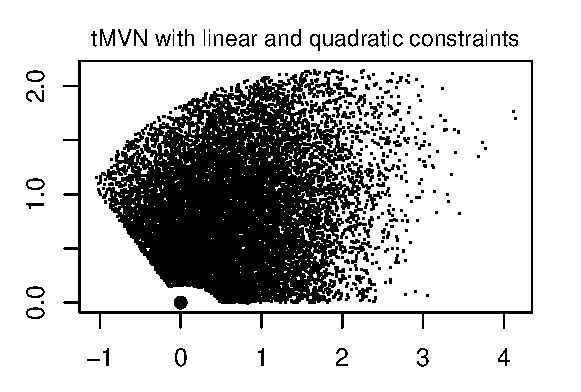
\includegraphics[scale=0.76]{tmvn_linear_quadratic_constr.eps}
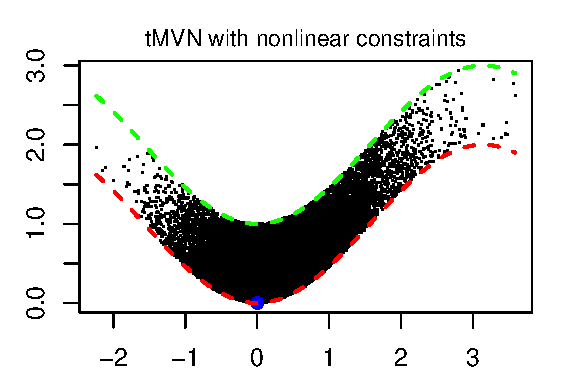
\includegraphics[scale=0.76]{tmvn_nonlinear_constr.eps}
\caption{Sampling 15,000 McMC samples from a bivariate Gaussian vector subject to linear and quadratic constraints (left panel), and to nonlinear constraints (right panel).}
\label{fig:tmvn}
\end{figure}





%\medskip
\section*{References}
\begin{enumerate}
	\item[{[1]}] Maatouk, Hassan \& Xavier Bay (2017). {\it Gaussian process emulators for computer experiments with inequality constraints}. Mathematical Geosciences 49(5):557-582.
	\item[{[2]}] Murray, Iain \& Ryan Prescott Adams \&  David J.C. MacKay (2010). {\it Elliptical slice sampling}. In: Proceedings of the thirteenth international conference on artificial intelligence and statistics, JMLR Workshop and Conference Proceedings, pp 541-548.
	\item[{[3]}] Pakman, Ari \& Liam Paninski (2014). {\it Exact Hamiltonian Monte Carlo for truncated multivariate Gaussians}. Journal of Computational and Graphical Statistics 23(2):518-542.
\end{enumerate}

\end{talk}

\begin{talk}
  {Copula-Based Regression with Discrete Covariates}% [1] talk title
  {Othmane Kortbi}% [2] speaker name
  {Department of Statistics and Business Analytics, UAE University, UAE}% [3] affiliations
  {okortbi@uaeu.ac.ae}% [4] email
  {} % [5] coauthors
{}{\timeslot{Thursday, August 22, 2024 -- Afternoon}{16:30}{17:00}{STC 0060}}{CS9-3}{CS9}

				% Insert the title of the special session if you were invited to give a talk in a special session.

In this project we investigated a new approach of estimating a regression function
based on copulas when covariates are mixture of continuous and discrete variables,
which is considered as an extension of Noh et al (2013) context. 
The main idea behind this approach is the writing of the regression function in terms of copula and marginal distributions,
thereafter we estimated the copula and marginal distributions. Now, since various 
methods are available in the literature to estimate both the copula and the marginals, this
approach offered us a rich and 
flexible alternative to many existing regression estimators.
We have studied the asymptotic behavior of the estimators obtained as well as the finite
sample performance of the estimators and illustrated their usefulness by analyzing real
data. An adapted algorithm is applied to construct copulas. Monte Carlo simulations are carried out 
to replicate datasets, estimate prediction model parameters and validate them.
 
\medskip


\begin{enumerate}

	
	\item[{[1]}] Crawley, M.J. (2005). {\it Statistics: An Introduction using R}. John Wiley \& Sons, Ltd.
	
	\item[{[2]}]Nelsen, R. B. (2006). {\it An introduction to copulas}. Springer Series in Statistics. Springer, New York.
	
	\item[{[3]}] Noh, H., Ghouch, A. E., and Bouezmarni, T. (2013). {\it Copula-based regression estimation and inference}. Journal of the American Statistical Association, 108(502), 676-688.
	
	\item[{[4]}] C. Ritz, C. and Streibig, J.C. (2008). {\it Nonlinear Regression in R}. Springer.

\item[{[5]}] Yan, J. (2007). {\it Enjoy the Joy of Copulas : With a Package copula}. Journal of Statistical Software, 21.

\end{enumerate}

\end{talk}

\begin{talk}
  {Geometric unification of central MCMC algorithms via rate distortion theory and factorizability of multivariate Markov chains}% [1] talk title
  {Michael Choi}% [2] speaker name
  {Department of Statistics and Data Science, National University of Singapore}% [3] affiliations
  {mchchoi@nus.edu.sg}% [4] email
  {Youjia Wang, Geoffrey Wolfer}% [5] coauthors
{MCMC: Convergence and Robustness}
{\timeslot{Friday, August 23, 2024 -- Morning}{10:30}{11:00}{STC 0020}}{SS1-1}{SS1}

				% Insert the title of the special session if you were invited to give a talk in a special session.

Motivated by the notion of mutual information between two random variables and rate distortion theory, we propose and analyze a rate distortion optimization problem for Markov chains based upon information divergences between transition matrices. This framework offers a unified variational view on the optimality of a comprehensive suite of MCMC algorithms such as Metropolis-Hastings, Glauber dynamics, swapping algorithm and Feynman-Kac path models. Along the way, we put forward an alternative notion of distance to independence, or more generally factorizability, of a given Markov chain on a finite product state space, which is of independent interest. We prove a counterpart of the Shearer's lemma governing the distance to independence and entropy rate of Markov chains and their information projections. In addition, we develop mixing and hitting time comparison results between the original chain and its information projections, as well as a Sanov's theorem in this context. These considerations eventually lead us to investigate the geometry of multivariate Markov chains induced by information divergences.
\end{talk}

\begin{talk}
  {A large deviation principle for Metropolis-Hastings sampling}% [1] talk title
  {Federica Milinanni}% [2] speaker name
  {KTH Royal Institute of Technology, Sweden}% [3] affiliations
  {fedmil@kth.se}% [4] email
  {Pierre Nyquist}% [5] coauthors
{MCMC: Convergence and Robustness}
{\timeslot{Friday, August 23, 2024 -- Morning}{11:00}{11:30}{STC 0020}}{SS1-2}{SS1}

				% Insert the title of the special session if you were invited to give a talk in a special session.
			
Sampling algorithms from the class of Markov chain Monte Carlo (MCMC) methods are widely used across scientific disciplines. Good performance measures are essential to analyse these methods, to compare different MCMC algorithms, and to tune parameters within a given method. Common tools that are used for analysing convergence properties of MCMC algorithms are, e.g., mixing times, spectral gap and functional inequalities (e.g. Poincaré, log-Sobolev). A further, rather novel, approach consists in the use of large deviations theory to study the convergence of empirical measures of MCMC chains. At the heart of large deviations theory is the large deviation principle, which allows us to describe the rate of convergence of the empirical measures through a so-called rate function.

In this talk we will consider Markov chains generated via MCMC methods of Metropolis-Hastings type for sampling from a target distribution on a Polish space. We will state a large deviation principle for the corresponding empirical measure, show examples of algorithms from this class for which the theorem applies, and illustrate how the result can be used to tune algorithms' parameters.

\medskip

\begin{enumerate}
	\item[{[1]}] Milinanni, F., \& Nyquist, P. (2024). A large deviation principle for the empirical measures of Metropolis–Hastings chains. \textit{Stochastic Processes and their Applications, 170}, 104293.
	\item[{[2]}] Milinanni, F., \& Nyquist, P. (2024). On the large deviation principle for Metropolis-Hastings Markov Chains: the Lyapunov function condition and examples. \textit{arXiv preprint arXiv:2403.08691.}
\end{enumerate}


\end{talk}

\begin{talk}
  {On the Convergence of MCMCs with Quantum Speedup}% [1] talk title
  {Ning Ning}% [2] speaker name
  {Texas A\&M University, College Station}% [3] affiliations
  {patning@tamu.edu}% [4] email
  {}% [5] coauthors
{MCMC: Convergence and Robustness}
{\timeslot{Friday, August 23, 2024 -- Morning}{11:30}{12:00}{STC 0020}}{SS1-3}{SS1}

				% Insert the title of the special session if you were invited to give a talk in a special session.

				
				

Quantum computing has emerged as a promising avenue for accelerating various computational tasks, including optimization and sampling problems. One particularly intriguing application lies in the realm of Markov Chain Monte Carlo (MCMC) algorithms, fundamental tools widely used in Bayesian inference, statistical physics, and machine learning. This talk delves into the convergence properties of MCMCs enhanced with quantum speedup. We investigate how quantum computing techniques can potentially expedite the convergence of MCMC algorithms, leading to more efficient sampling from complex probability distributions. 
%Our analysis encompasses theoretical frameworks and practical considerations, shedding light on the interplay between quantum mechanics and stochastic processes. 
We explore key theoretical concepts underlying quantum-enhanced MCMCs, examining the impact of quantum resources on convergence rates and sampling quality.
\end{talk}

\begin{talk}
  {Adapting the Stereographic Bouncy Particle Sampler}% [1] talk title
  {Cameron Bell}% [2] speaker name
  {University of Warwick, UK}% [3] affiliations
  {cameron.bell@warwick.ac.uk}% [4] email
  {Krzysztof {\L}atuszy{\'n}ski and Gareth O. Roberts}% [5] coauthors
{MCMC: Convergence and Robustness}
{\timeslot{Friday, August 23, 2024 -- Morning}{12:00}{12:30}{STC 0020}}{SS1-4}{SS1}

				% Insert the title of the special session if you were invited to give a talk in a special session.
			

In order to tackle the problem of sampling from heavy tailed, high dimensional distributions via Markov Chain Monte Carlo (MCMC) methods, Yang, {\L}atuszy{\'n}ski and Roberts (2022) introduces the stereographic projection as a tool to compactify $\mathbb{R}^d$ and transform the problem into sampling from a density on the unit sphere $\mathbb{S}^d$. The MCMC algorithms (a random walk Metropolis algorithm and a bouncy particle sampler) presented in that paper are shown to be uniformly ergodic, even for certain polynomial-tailed target distributions, where Euclidean MCMC algorithms result in chains that are not even geometrically ergodic. Furthermore, robustness properties are provided to show that these stereographic MCMC algorithms perform at least as well as their Euclidean counterparts in terms of asymptotic variance of estimator. In the best case scenario, they exhibit a ``blessing of dimensionality" which allows them to return to the high probability region faster as the dimension increases. However, the improvement in algorithmic efficiency, as well as the computational cost of the implementation, are still significantly impacted by the parameters used in this transformation (which provide an affine preconditioning of $\mathbb{R}^d$).

We introduce an adaptive version of the Stereographic Bouncy Particle Sampler (SBPS) which automatically updates the parameters of the algorithm as the run progresses. The adaptive setup allows us to better exploit the power of the stereographic projection, even when the initial parameters are poorly chosen.

Leveraging the simultaneous uniform ergodicity of the SBPS and the Adapting Increasingly Rarely framework (Chimisov, {\L}atuszy{\'n}ski and Roberts (2018)), we establish a novel framework for proving convergence of continuous time adaptive MCMC algorithms which allow us to prove LLNs and a CLT for the adaptive SBPS. We demonstrate the ability of the adaptive SBPS algorithm in several simulation studies, such as estimating tail probabilities of heavy tailed, high dimensional target distributions, which show that it can outperform algorithms such as HMC in these settings.

\begin{enumerate}
	\item[{[1]}] Yang, Jun, {\L}atuszy{\'n}ski, Krzysztof and Roberts, Gareth O. (2022). {\it Stereographic Markov Chain Monte Carlo}. arXiv preprint arXiv:2205.12112.
	\item[{[2]}] Chimisov, Cyril, {\L}atuszy{\'n}ski, Krzysztof and Roberts, Gareth O. (2018). {\it Air Markov chain Monte Carlo}. arXiv preprint arXiv:1801.09309.
\end{enumerate}
\end{talk}

\begin{talk}
  {Losing momentum in continuous-time stochastic optimisation}% [1] talk title
  {Jonas Latz}% [2] speaker name
  {University of Manchester}% [3] affiliations
  {jonas.latz@manchester.ac.uk}% [4] email
  {Kexin Jin, Chenguang Liu, Alessandro Scagliotti}% [5] coauthors
{Continuous-time dynamics in Monte Carlo and beyond}
{\timeslot{Friday, August 23, 2024 -- Morning}{10:30}{11:00}{STC 0040}}{SS17-1}{SS17}

				% Insert the title of the special session if you were invited to give a talk in a special session.
			
The training of deep neural networks and other modern machine learning models usually consists in solving non-convex optimisation problems that are high-dimensional and subject to large-scale data. Here, momentum-based stochastic optimisation algorithms have become especially popular in recent years. The stochasticity arises from data subsampling which reduces computational cost. Moreover, both, momentum and stochasticity are supposed to help the algorithm to overcome local minimisers and, hopefully, converge globally. Theoretically, this combination of stochasticity and momentum is badly understood.

In our work [1], we propose and analyse a continuous-time model for stochastic gradient descent with momentum. This model is a piecewise-deterministic Markov process that represents the particle movement by an underdamped dynamical system and the data subsampling through a stochastic switching of the dynamical system. In our analysis, we investigate longtime limits, the subsampling-to-no-subsampling limit, and the momentum-to-no-momentum limit. We are particularly interested in the case of reducing the momentum over time: intuitively, the momentum helps to overcome local minimisers in the initial phase of the algorithm, but prohibits fast convergence to a global minimiser later. Under convexity assumptions, we show convergence of our dynamical system to the global minimiser when reducing momentum over time and let the subsampling rate go to infinity.

We then propose a stable, symplectic discretisation scheme to construct an algorithm from our continuous-time dynamical system. In numerical experiments, we study our discretisation scheme in convex and non-convex test problems. Additionally, we train a convolutional neural network to solve the CIFAR-10 image classification problem. Here, our algorithm reaches competitive results compared to stochastic gradient descent with momentum.

\medskip

\begin{enumerate}
	\item[{[1]}] Jin, Kexin, Jonas Latz, Chenguang Liu, \& Alessandro Scagliotti (2022). Losing momentum in continuous-time stochastic optimisation. arXiv:2209.03705.
\end{enumerate}

\end{talk}

\begin{talk}
  {How to choose an annealing algorithm}% [1] talk title
  {Alexandre Bouchard-C\^ot\'e}% [2] speaker name
  {University of British Columbia}% [3] affiliations
  {bouchard@stat.ubc.ca}% [4] email
  {Saifuddin Syed, Kevin Chern, Arnaud Doucet}% [5] coauthors
{Continuous-time dynamics in Monte Carlo and beyond}
{\timeslot{Friday, August 23, 2024 -- Morning}{11:00}{11:30}{STC 0040}}{SS17-2}{SS17}

				% Insert the title of the special session if you were invited to give a talk in a special session.

				
				

Over the years, several algorithms have been developed to tackle normalization constant estimation. A handful of those have passed the test of time thanks to their capacity to beat the curse of dimensionality in many realistic scenarios: on one hand, Annealed Importance Sampling (AIS) and Sequential Monte Carlo (SMC) methods, and on the other, Parallel Tempering (PT) and Simulated Tempering (ST) algorithms. Indeed many recent developments can be contextualized as members of one of these two families of meta-algorithms.

A priori, these two families of algorithms, AIS/SMC versus PT/ST, appear quite distinct and indeed these communities are largely silos. This leads to an important practical question: for a given problem, which annealing algorithm should be recommended? I will present our work toward tackling this question, in which a key object needed for theoretical and methodological purposes is the rate function of various limiting PDMPs. 
\end{talk}

\begin{talk}
  {Projected ensemble data assimilation}% [1] talk title
  {S. B. Dubinkina }% [2] speaker name
  {Amsterdam Center for Dynamics and Computation, the Department of Mathematics, VU Amsterdam, The Netherlands}% [3] affiliations
  {s.b.dubinkina@vu.nl}% [4] email
  {J. de Wiljes}% [5] coauthors
{Continuous-time dynamics in Monte Carlo and beyond}
{\timeslot{Friday, August 23, 2024 -- Morning}{11:30}{12:00}{STC 0040}}{SS17-3}{SS17}

				% Insert the title of the special session if you were invited to give a talk in a special session.
			
Ensemble data assimilation is unable to reduce the error estimate for high-dimensional systems when used with small ensemble size. A typical remedy is dimesion reduction by localization. Though localization reduces the error substantially for both linear and nonlinear data-assimilation methods, the former ones considerably outperform the latter ones in a quasi-linear regime. We propose a further dimension reduction based on projection and show substantial error decrease of a nonlinear data-assimilation method in a challenging data-assimilation setup with small ensemble size and ample observations.  

\medskip

\end{talk}

\begin{talk}
  {Function space embeddings for non-tensor product spaces and application to high-dimensional approximation}% [1] talk title
  {Michael Gnewuch}% [2] speaker name
  {University of Osnabr\"uck}% [3] affiliations
  {michael.gnewuch@uos.de}% [4] email
  {Peter Kritzer, Klaus Ritter}% [5] coauthors
{Function spaces and algorithms for high-dimensional problems}
{\timeslot{Friday, August 23, 2024 -- Morning}{10:30}{11:00}{STC 0050}}{SS24-1}{SS24}

				% Insert the title of the special session if you were invited to give a talk in a special session.
			
%Your abstract goes here. Please do not use your own commands or macros.
%Embeddings of (scales of) function spaces are helpful tools to transfer the analysis of algorithms from 


%In this talk we want to discuss a general approach 

%In the analysis of high-dimensional problems 

In tractability analysis one is interested in continuous approximation problems
that are defined on a scale of function spaces $(H_d)_{d\in {\mathbb N}}$, where the parameter
$d$ typically denotes the number of variables the functions in $H_d$ depend on.
An important goal is to find algorithms that scale well with respect to the dimension parameter $d$ and help to break the curse of dimensionality. 
Some specific features of the function spaces can be very helpful for the analysis of certain types of algorithms; e.g., for the analysis of unbiased randomized algorithms it may be extremely helpful if the norm on $H_d$ induces an ANOVA decomposition on $H_d$, which can be used to analyze the error ($=$ variance) of the algorithms. 
In general, a suitable embedding of scales of function spaces may help to transfer results from scales of function spaces with favourable features to other scales of interest. There are several general embedding results known in the case where $H_d$ is the $d$-fold tensor product of a reproducing kernel Hilbert space (RKHS) 
$H_1$; examples include weighted RKHSs where the weights are product weights and so-called spaces of increasing smoothness.
%, cf., e.g., [1] and [2]. 

In this talk we discuss a general embedding approach that still works in the case where $H_d$ is not necessarily of tensor product form. This is, e.g., the case if we consider weighted RKHSs, where the weights are product and order-dependent weights or finite-order weights. As an application we study $L^\infty$-approximation on a RKHS of functions that depend on infinitely many variables (which can be viewed as a limiting case of tractability analysis).



\medskip

%If you would like to include references, please do so by creating a simple list numbered by [1], [2], [3], \ldots. See example below.
%Please do not use the \texttt{bibliography} environment or \texttt{bibtex} files.
%APA reference style is recommended.

%\begin{enumerate}
%	\item[{[1]}] M. Gnewuch, M. Hefter, A. Hinrichs, and K. Ritter. Embeddings of %weighted Hilbert spaces and applications to multivariate and infinite-dimensional %integration, J. Approx. Theory, 222 (2017), 8--39. 
%	\item[{[2]}] M. Gnewuch, M. Hefter, A. Hinrichs, K. Ritter, and G. W. Wasilkowski. Embeddings for  infinite-dimensional integration and $L_2$-approximation with increasing smoothness, J. Complexity, 54 (2019), 101406, 1--32. 
%\end{enumerate}

%Equations may be used if they are referenced. Please note that the equation numbers may be different (but will be cross-referenced correctly) in the final program book.
\end{talk}

\begin{talk}
  {ANOVA-boosting for high-dimensional approximation}% [1] talk title
  {Laura Weidensager}% [2] speaker name
  {Chemnitz University of Technology}% [3] affiliations
  {laura.weidensager@math.tu-chemnitz.de}% [4] email
  {Daniel Potts}% [5] coauthors
{Function spaces and algorithms for high-dimensional problems}
{\timeslot{Friday, August 23, 2024 -- Morning}{11:00}{11:30}{STC 0050}}{SS24-2}{SS24}

				% Insert the title of the special session if you were invited to give a talk in a special session.

				
				
We study the problem of scattered-data approximation on $\mathbb{R}^d$, where we have given sample points and the corresponding function evaluations of a function $f$. The random Fourier feature approach is a two-layer network with a randomized but fixed single hidden layer. The output layer is trained. In this talk we present algorithms from [1], which aim to adapt the randomized hidden layer to the function $f$.\par
We use the analysis of variance (ANOVA) decomposition 
$$f(\mathbf{ x}) = \sum_{\mathbf{ u}\subseteq \{1,\ldots, d\}} f_{\mathbf{ u}}(\mathbf{ x}_{\mathbf{\mathbf{ u}}})$$
for approximating high-dimensional functions of low effective dimension. Thereby we give a relation between the Fourier transform of the function $f$ and the ANOVA terms $f_{\mathbf{u}}$. \par
In the case for dependent input variables, the ANOVA decomposition is generalized with the aim to detect the structure of the function. We use a least-squares algorithm with a regularization which penalizes the non-orthogonality of ANOVA terms to find which input variables and variable interactions are important. This information is then used to boost random Fourier feature algorithms. 

\medskip

[1] Potts, D., Weidensager, L. ANOVA-boosting for Random Fourier Features, \textit{ArXiv e-print: 2404.03050}, 2024\\
\end{talk}

\begin{talk}
  {Tractability results for integration on Gaussian spaces}% [1] talk title
  {Robin Rüßmann}% [2] speaker name
  {RPTU Kaiserslautern}% [3] affiliations
  {ruessmann@mathematik.uni-kl.de}% [4] email
  {Michael Gnewuch, Klaus Ritter}% [5] coauthors
{Function spaces and algorithms for high-dimensional problems}
{\timeslot{Friday, August 23, 2024 -- Morning}{11:30}{12:00}{STC 0050}}{SS24-3}{SS24}

				% Insert the title of the special session if you were invited to give a talk in a special session.
			
We study integration with respect to the $d$-dimensional standard normal distribution on Gaussian spaces. Here, given shape parameters $\sigma_j>0$, a Gaussian space is a reproducing kernel Hilbert space, whose kernel is defined by $L_{\boldsymbol{\sigma}}(x,y)=\prod_{j=1}^d \exp(-\sigma_j^2(x_j-y_j)^2)$.  

We give new tractability results based on the asymptotic behavior of $\sigma_j$ as $j$ tends to infinity. Positive results are obtained both from previously established algorithms, as well as a new transference principle between Gaussian spaces and Hermite spaces.   

\end{talk}

\begin{talk}
  {Unbiased and Multilevel Methods for a Class of Diffusions Partially Observed via Marked Point Processes}% [1] talk title
  {Miguel Alvarez}% [2] speaker name
  {King Abdullah University of Science and Technology (KAUST)}% [3] affiliations
  {miguelangel.alvarezballesteros@kaust.edu.sa}% [4] email
  {Ajay Jasra, Hamza Ruzayqat}% [5] coauthors
{}{\timeslot{Friday, August 23, 2024 -- Morning}{10:30}{11:00}{STC 0060}}{CS11-1}{CS11}

				% Insert the title of the special session if you were invited to give a talk in a special session.
			
In this talk we consider the filtering problem associated to partially observed diffusions, with observations following a marked point process.
In the model, the data form a point process with observation times that have its intensity driven by a diffusion, with the associated marks also depending upon the diffusion process.
We assume that one must resort to time-discretizing the diffusion process and develop particle and multilevel particle filters to recursively approximate the filter.
In particular, we prove that our multilevel particle filter can achieve a mean square error (MSE) of $\mathcal{O}(\epsilon^2)$ ($\epsilon>0$ and arbitrary) with a cost
of $\mathcal{O}(\epsilon^{-2.5})$ versus using a particle filter which has a cost of $\mathcal{O}(\epsilon^{-3})$ to achieve the same MSE. We then show how this methodology can be extended to give unbiased (that is with no time-discretization error) estimators of the filter, which are proved to have finite variance and with high-probability have finite cost. Finally, we extend our methodology to the problem of online static-parameter estimation.

\medskip

\end{talk}

\begin{talk}
 {Multilevel optimization-based sampling for large-scale inverse problems}% [1] talk title
  {Chuntao Chen}% [2] speaker name
  {Lappeenranta University of Technology}% [3] affiliations
  {Chuntao.Chen@lut.fi}% [4] email
  {Tiangang Cui, Youssef Marzouk}% [5] coauthors
{}{\timeslot{Friday, August 23, 2024 -- Morning}{11:00}{11:30}{STC 0060}}{CS11-2}{CS11}

				% Insert the title of the special session if you were invited to give a talk in a special session.
			
We combine the Multilevel Monte Carlo and the optimization-based samplers, including Randomized-and-Then-Optimize (RTO) and Implicit Sampling, to address the challenges that classical MCMC faces, and implements the samplers in computationally costly Bayesian inverse problems including an ODE model and a PDE problem. Simulations using the optimization-based samplers like RTO can be parallelized which allows us to develop efficient
MCMC algorithms or self-normalizing estimators to solve the inverse problems. Multilevel Monte Carlo is proven to significantly reduce the computational cost of Monte Carlo simu-
lation, which helps us further improve the RTO method. To adapt the multilevel method on the optimization-based samplers, we develop the complexity theorem for multilevel self-normalizing estimators. The corresponding numerical experiments produce good results on RTO method, showing a high effective sample ratio in the importance sampling scheme, and the variances of the self-normalizing estimators converge when discretization size decreases.


\medskip




\end{talk}

\begin{talk}
  {Single-ensemble multilevel Monte Carlo for discrete interacting-particle methods}% [1] talk title
  {Arne Bouillon}% [2] speaker name
  {KU Leuven}% [3] affiliations
  {arne.bouillon@kuleuven.be}% [4] email
  {Toon Ingelaere, Giovanni Samaey}% [5] coauthors
{}{\timeslot{Friday, August 23, 2024 -- Morning}{11:30}{12:00}{STC 0060}}{CS11-3}{CS11}

				% Insert the title of the special session if you were invited to give a talk in a special session.

Interacting-particle methods have found applications in domains such as filtering, optimization and posterior sampling. These parallelizable and often gradient-free algorithms use an ensemble of particles that evolve in time, based on the combination of well-chosen dynamics and interaction between the particles. For computationally expensive dynamics -- for example, Bayesian inversion with an expensive forward model or optimization of an expensive objective function -- the cost of attaining a high accuracy quickly becomes prohibitive.

In this talk, we discuss our recent work [1], in which we exploit a hierarchy of approximations to this forward model and apply multilevel Monte Carlo (MLMC) techniques. More specifically, we extend the approach suggested in [2, 3] for the ensemble Kalman filter: we use MLMC at each time step to estimate the interaction term within a single, globally-coupled ensemble. We formulate conditions on the method dynamics, interaction term, and forward model, under which we prove an asymptotic bound on the cost-to-error relation. This bound suggests that a multilevel simulation strategy is more efficient than a single-level one for a large family of interacting-particle methods. Numerical experiments corroborate our analysis of the improved asymptotic cost-to-error rate.

\medskip

[1] A. Bouillon, T. Ingelaere, G. Samaey, Single-ensemble multilevel Monte Carlo for discrete interacting-particle methods, in preparation.

[2] H. Hoel, K. J. H. Law, and R. Tempone, Multilevel ensemble Kalman filtering, SIAM J. Numer. Anal., 54 (2016), pp.\ 1813--1839.

[3] A. Chernov, H. Hoel, K. J. H. Law, F. Nobile, and R. Tempone, Multilevel ensemble Kalman filtering for spatio-temporal processes, Numer. Math., 147 (2021), pp.\ 71--125.
\end{talk}



\iffalse
\begin{talk}
 {Talk title \#1}% [1] talk title
 {Awesome Speaker \#1}% [2] speaker name
 {Nice University \#1}% [3] affiliations
 {good.email@gooduni.ca}% [4] email
 {co-author 2, co-author 3}% [5] coauthors
 {This is a TWO-PART session}% [6] special session title
 {\timeslot{Monday, July 18, 2022}{15:30}{16:00}{Lecture Hall 4}}% [7] time slot
 {2011}% [8] talk id
 {2010}% [9] session id
Abstract goes here.
\end{talk}

\begin{talk}
	{Talk title \#2}% [1] talk title
	{Awesome Speaker \#2}% [2] speaker name
	{Nice University \#2}% [3] affiliations
	{good.email@gooduni.ca}% [4] email
	{}% [5] coauthors
	{This is a TWO-PART session}% [6] special session title
	{\timeslot{Monday, July 18, 2022}{15:30}{16:00}{Lecture Hall 4}}% [7] time slot
	{2012}% [8] talk id
	{2010}% [9] session id
	Abstract goes here.
\end{talk}

\begin{talk}
	{Talk title \#3}% [1] talk title
	{Awesome Speaker \#3}% [2] speaker name
	{Nice University \#3}% [3] affiliations
	{good.email@gooduni.ca}% [4] email
	{co-author 2, co-author 3}% [5] coauthors
	{This is a TWO-PART session}% [6] special session title
	{\timeslot{Monday, July 18, 2022}{15:30}{16:00}{Lecture Hall 4}}% [7] time slot
	{2013}% [8] talk id
	{2010}% [9] session id
	Abstract goes here.
\end{talk}

\begin{talk}
	{Talk title \#4}% [1] talk title
	{Awesome Speaker \#4}% [2] speaker name
	{Nice University \#4}% [3] affiliations
	{good.email@gooduni.ca}% [4] email
	{co-author 2, co-author 3}% [5] coauthors
	{This is a TWO-PART session}% [6] special session
	{\timeslot{Monday, July 18, 2022}{15:30}{16:00}{Lecture Hall 4}}% [7] time slot
	{2014}% [8] talk id
	{2010}% [9] session id
	Abstract goes here.
\end{talk}


\begin{talk}
	{Talk title \#5}% [1] talk title
	{Awesome Speaker \#5}% [2] speaker name
	{Nice University \#5}% [3] affiliations
	{good.email@gooduni.ca}% [4] email
	{co-author 2, co-author 3}% [5] coauthors
	{This is a TWO-PART session}% [6] special session title
	{\timeslot{Monday, July 18, 2022}{15:30}{16:00}{Lecture Hall 4}}% [7] time slot
	{2021}% [8] talk id
	{2020}% [9] session id
	Abstract goes here.
\end{talk}

\begin{talk}
	{Talk title \#6}% [1] talk title
	{Awesome Speaker \#6}% [2] speaker name
	{Nice University \#6}% [3] affiliations
	{good.email@gooduni.ca}% [4] email
	{}% [5] coauthors
	{This is a SINGLE-PART session}% [6] special session title
	{\timeslot{Monday, July 18, 2022}{15:30}{16:00}{Lecture Hall 4}}% [7] time slot
	{2022}% [8] talk id
	{2020}% [9] session id
	Abstract goes here.
\end{talk}

\begin{talk}
	{Talk title \#7}% [1] talk title
	{Awesome Speaker \#7}% [2] speaker name
	{Nice University \#7}% [3] affiliations
	{good.email@gooduni.ca}% [4] email
	{co-author 2, co-author 3}% [5] coauthors
	{This is a TWO-PART session}% [6] special session title
	{\timeslot{Monday, July 18, 2022}{15:30}{16:00}{Lecture Hall 4}}% [7] time slot
	{2023}% [8] talk id
	{2020}% [9] session id
	Abstract goes here.
\end{talk}

\begin{talk}
	{Talk title \#8}% [1] talk title
	{Awesome Speaker \#8}% [2] speaker name
	{Nice University \#8}% [3] affiliations
	{good.email@gooduni.ca}% [4] email
	{co-author 2, co-author 3}% [5] coauthors
	{This is a TWO-PART session}% [6] special session
	{\timeslot{Monday, July 18, 2022}{15:30}{16:00}{Lecture Hall 4}}% [7] time slot
	{2024}% [8] talk id
	{2020}% [9] session id
	Abstract goes here.
\end{talk}

\begin{talk}
	{Talk title \#9}% [1] talk title
	{Awesome Speaker \#9}% [2] speaker name
	{Nice University \#9}% [3] affiliations
	{good.email@gooduni.ca}% [4] email
	{co-author 2, co-author 3}% [5] coauthors
	{This is a TWO-PART session}% [6] special session title
	{\timeslot{Monday, July 18, 2022}{15:30}{16:00}{Lecture Hall 4}}% [7] time slot
	{2025}% [8] talk id
	{2020}% [9] session id
	Abstract goes here.
\end{talk}

\begin{talk}
	{Talk title \#10}% [1] talk title
	{Awesome Speaker \#10}% [2] speaker name
	{Nice University \#10}% [3] affiliations
	{good.email@gooduni.ca}% [4] email
	{}% [5] coauthors
	{This is a TWO-PART session}% [6] special session title
	{\timeslot{Monday, July 18, 2022}{15:30}{16:00}{Lecture Hall 4}}% [7] time slot
	{2026}% [8] talk id
	{2020}% [9] session id
	Abstract goes here.
\end{talk}

\begin{talk}
	{Talk title \#11}% [1] talk title
	{Awesome Speaker \#11}% [2] speaker name
	{Nice University \#11}% [3] affiliations
	{good.email@gooduni.ca}% [4] email
	{co-author 2, co-author 3}% [5] coauthors
	{This is a TWO-PART session}% [6] special session title
	{\timeslot{Monday, July 18, 2022}{15:30}{16:00}{Lecture Hall 4}}% [7] time slot
	{2027}% [8] talk id
	{2020}% [9] session id
	Abstract goes here.
\end{talk}

\begin{talk}
	{Talk title \#12}% [1] talk title
	{Awesome Speaker \#12}% [2] speaker name
	{Nice University \#12}% [3] affiliations
	{good.email@gooduni.ca}% [4] email
	{co-author 2, co-author 3}% [5] coauthors
	{}% [6] special session title
	{\timeslot{Monday, July 18, 2022}{15:30}{16:00}{Lecture Hall 4}}% [7] time slot
	{3001}% [8] talk id
	{}% [9] session id
	Abstract goes here.
\end{talk}

\section{Contributed Talks}

\begin{talk}
	{Talk title \#13}% [1] talk title
	{Awesome Speaker \#13}% [2] speaker name
	{Nice University \#13}% [3] affiliations
	{good.email@gooduni.ca}% [4] email
	{co-author 2, co-author 3}% [5] coauthors
	{}% [6] special session title
	{\timeslot{Monday, July 18, 2022}{15:30}{16:00}{Lecture Hall 4}}% [7] time slot
	{3002}% [8] talk id
	{}% [9] session id
	Abstract goes here.
\end{talk}

\begin{talk}
	{Talk title \#14}% [1] talk title
	{Awesome Speaker \#14}% [2] speaker name
	{Nice University \#14}% [3] affiliations
	{good.email@gooduni.ca}% [4] email
	{co-author 2, co-author 3}% [5] coauthors
	{}% [6] special session title
	{\timeslot{Monday, July 18, 2022}{15:30}{16:00}{Lecture Hall 4}}% [7] time slot
	{3003}% [8] talk id
	{}% [9] session id
	Abstract goes here.
\end{talk}

\begin{talk}
	{Talk title \#15}% [1] talk title
	{Awesome Speaker \#15}% [2] speaker name
	{Nice University \#15}% [3] affiliations
	{good.email@gooduni.ca}% [4] email
	{co-author 2, co-author 3}% [5] coauthors
	{}% [6] special session title
	{\timeslot{Monday, July 18, 2022}{15:30}{16:00}{Lecture Hall 4}}% [7] time slot
	{3004}% [8] talk id
	{}% [9] session id
	Abstract goes here.
\end{talk}

\fi   % old
\chapter{Special Sessions}

\begin{session}
 {Stochastic Computation and Complexity, Part I}% [1] session title
 {Stefan Heinrich}% [2] organizer one name
 {RPTU Kaiserslautern-Landau}% [3] organizer one affiliations
 {heinrich@informatik.uni-kl.de}% [4] organizer one email
 {Thomas M\"uller-Gronbach}% [5] organizer two name. Leave unchanged if there is no second organizer, otherwise fill in accordingly.
 {University of Passau}% [6] affiliations. Leave unchanged if there is no second organizer, otherwise fill in accordingly.
 {Thomas.Mueller-Gronbach@uni-passau.de}% [7] email. Leave unchanged if there is no second organizer, otherwise fill in accordingly.
 {S1}% [8] session id
 {\thirdorganizer{Larisa Yaroslavtseva}{University of Graz}{larisa.yaroslavtseva@uni-graz.at}}% [9] third organizer, if any

 The session is devoted to algorithms and complexity for
 quadrature and strong approximation of SDEs and SPDEs, in particular under nonstandard assumptions,
 high and infinite dimensional integration and approximation, and
 stochastic optimization and neural networks,
 including connections to functional analysis and stochastic analysis.
 \medskip
\end{session}

\sessionPart{}% [1] part
{\hfill\timeslot{Mon, July 28, 2024 -- Morning}
{10:30}{12:30} % Start and End time
{}} % Room 
\sessionTalk{Quantitative approximation of stochastic kinetic equations: from discrete to continuum}
{Chengcheng Ling}
{S1-1}
\sessionTalk{A strong order 1.5 boundary preserving discretization scheme for scalar SDEs defined in a domain}
{Andreas Neuenkirch}
{S1-2}
\sessionTalk{An adaptive Milstein-type method for strong approximation of systems of SDEs with a discontinuous drift coefficient}
{Christopher Rauhögger}
{S1-3}
\sessionTalk{Stong order 1 adaptive approximation of jump-diffusion SDEs with discontinuous drift}
{Verena Schwarz}
{S1-4}


\clearpage

\begin{session}
 {Nested expectations: models and estimators, Part I}% [1] session title
 {Arved Bartuska}% [2] organizer one name
 {King Abdullah University of Science and Technology and RWTH Aachen University}% [3] organizer one affiliations
 {sarved.bartuska@kaust.edu.sa}% [4] organizer one email
 {Abdul-Lateef Haji-Ali}% [5] organizer two name. Leave unchanged if there is no second organizer, otherwise fill in accordingly.
 {Heriot-Watt University}% [6] affiliations. Leave unchanged if there is no second organizer, otherwise fill in accordingly.
 {a.hajiali@hw.ac.uk}% [7] email. Leave unchanged if there is no second organizer, otherwise fill in accordingly.
 {S3}% [8] session id
{}

 Nested expectations
 arise in many applications, such as in engineering, mathematical finance, and medical decision-making. In addition to their nested structure, numerical estimations of such expectations are often complicated by singularities or discontinuities. Moreover, approximations when evaluating inner expectations using, for example, finite element or time-stepping schemes render traditional estimation methods such as double-loop Monte Carlo prohibitively expensive. This session will explore models and applications with this structure and methods for efficient estimation.
\end{session}

\sessionPart{}% [1] part
{\hfill\timeslot{Mon, Jul 28, 2025 -- Morning}
{10:30}{12:30} % Start and End time
{PH Auditorium}} % Room 
\sessionTalk{An Adaptive Sampling Algorithm for Level-set Approximation}
{Abdul Lateef Haji Ali}
{S3-1}
\sessionTalk{Posterior-Free A-Optimal Bayesian Design of Experiments via Conditional Expectation}
{Vinh Hoang}
{S3-2}
\sessionTalk{QMC for Bayesian optimal experimental design with application to inverse problems governed by PDEs}
{Vesa Kaarnioja}
{S3-3}


\clearpage

\begin{session}
 {Stochastic Computation and Complexity, Part II}% [1] session title
 {Stefan Heinrich}% [2] organizer one name
 {RPTU Kaiserslautern-Landau}% [3] organizer one affiliations
 {heinrich@informatik.uni-kl.de}% [4] organizer one email
 {Thomas M\"uller-Gronbach}% [5] organizer two name. Leave unchanged if there is no second organizer, otherwise fill in accordingly.
 {University of Passau}% [6] affiliations. Leave unchanged if there is no second organizer, otherwise fill in accordingly.
 {Thomas.Mueller-Gronbach@uni-passau.de}% [7] email. Leave unchanged if there is no second organizer, otherwise fill in accordingly.
 {S5}% [8] session id
 {\thirdorganizer{Larisa Yaroslavtseva}{University of Graz}{larisa.yaroslavtseva@uni-graz.at}}% [9] third organizer, if any

 The session is devoted to algorithms and complexity for
 quadrature and strong approximation of SDEs and SPDEs, in particular under nonstandard assumptions,
 high and infinite dimensional integration and approximation, and
 stochastic optimization and neural networks,
 including connections to functional analysis and stochastic analysis.
 \medskip
\end{session}

\sessionPart{}% [1] part
{\hfill\timeslot{Mon, Jul 28, 2025 -- Afternoon}
{15:30}{17:30} % Start and End time
{HH Auditorium}} % Room 
\sessionTalk{Optimality of deterministic and randomized QMC-cubatures on several scales of function spaces}
{Michael Gnewuch}
{S5-1}
\sessionTalk{Optimal designs for function discretization and construction of tight frames}
{Kateryna Pozharska}
{S5-2}
\sessionTalk{Complexity of approximating piecewise smooth functions in the presence of deterministic or random noise}
{Leszek Plaskota}
{S5-3}


\clearpage

\begin{session}
 {Stochastic Computation and Complexity, Part III}% [1] session title
 {Stefan Heinrich}% [2] organizer one name
 {RPTU Kaiserslautern-Landau}% [3] organizer one affiliations
 {heinrich@informatik.uni-kl.de}% [4] organizer one email
 {Thomas M\"uller-Gronbach}% [5] organizer two name. Leave unchanged if there is no second organizer, otherwise fill in accordingly.
 {University of Passau}% [6] affiliations. Leave unchanged if there is no second organizer, otherwise fill in accordingly.
 {Thomas.Mueller-Gronbach@uni-passau.de}% [7] email. Leave unchanged if there is no second organizer, otherwise fill in accordingly.
 {S8}% [8] session id
 {\thirdorganizer{Larisa Yaroslavtseva}{University of Graz}{larisa.yaroslavtseva@uni-graz.at}}% [9] third organizer, if any

 The session is devoted to algorithms and complexity for
 quadrature and strong approximation of SDEs and SPDEs, in particular under nonstandard assumptions,
 high and infinite dimensional integration and approximation, and
 stochastic optimization and neural networks,
 including connections to functional analysis and stochastic analysis.
 \medskip
\end{session}

\sessionPart{}% [1] part
{\hfill\timeslot{Tue, Jul 29, 2025 -- Morning}
{10:30}{12:30} % Start and End time
{HH Auditorium}} % Room 
\sessionTalk{Computing the stationary measure of McKean-Vlasov SDEs}
{Jean-François Chassagneux}
{S8-1}
\sessionTalk{On the convergence of the Euler-Maruyama scheme for McKean-Vlasov SDEs}
{Noufel Frikha}
{S8-3}
\sessionTalk{Wasserstein Convergence of Score-based Generative Models under Semiconvexity and Discontinuous Gradients}
{Sotirios Sabanis}
{S8-4}


\clearpage

\begin{session}
 {Stochastic Computation and Complexity, Part IV}% [1] session title
 {Stefan Heinrich}% [2] organizer one name
 {RPTU Kaiserslautern-Landau}% [3] organizer one affiliations
 {heinrich@informatik.uni-kl.de}% [4] organizer one email
 {Thomas M\"uller-Gronbach}% [5] organizer two name. Leave unchanged if there is no second organizer, otherwise fill in accordingly.
 {University of Passau}% [6] affiliations. Leave unchanged if there is no second organizer, otherwise fill in accordingly.
 {Thomas.Mueller-Gronbach@uni-passau.de}% [7] email. Leave unchanged if there is no second organizer, otherwise fill in accordingly.
 {S12}% [8] session id
 {\thirdorganizer{Larisa Yaroslavtseva}{University of Graz}{larisa.yaroslavtseva@uni-graz.at}}% [9] third organizer, if any

 The session is devoted to algorithms and complexity for
 quadrature and strong approximation of SDEs and SPDEs, in particular under nonstandard assumptions,
 high and infinite dimensional integration and approximation, and
 stochastic optimization and neural networks,
 including connections to functional analysis and stochastic analysis.
 \medskip
\end{session}

\sessionPart{}% [1] part
{\hfill\timeslot{Tue, Jul 29, 2025 -- Afternoon}
{15:30}{17:30} % Start and End time
{}} % Room 
\sessionTalk{Optimal strong approximation of SDEs with H\"older continuous drift coefficient}
{Larisa Yaroslavtseva}
{S12-1}
\sessionTalk{Malliavin Differentiation of Lipschitz SDEs and BSDEs and an Application to Quadratic Forward-Backward SDEs}
{Alexander Steinicke}
{S12-2}
\sessionTalk{Tractability of $L_2$-approximation and integration in weighted Hermite spaces of finite smoothness}
{Gunther Leobacher}
{S12-3}


\clearpage

\begin{session}
 {Stochastic Computation and Complexity, Part V}% [1] session title
 {Stefan Heinrich}% [2] organizer one name
 {RPTU Kaiserslautern-Landau}% [3] organizer one affiliations
 {heinrich@informatik.uni-kl.de}% [4] organizer one email
 {Thomas M\"uller-Gronbach}% [5] organizer two name. Leave unchanged if there is no second organizer, otherwise fill in accordingly.
 {University of Passau}% [6] affiliations. Leave unchanged if there is no second organizer, otherwise fill in accordingly.
 {Thomas.Mueller-Gronbach@uni-passau.de}% [7] email. Leave unchanged if there is no second organizer, otherwise fill in accordingly.
 {S16}% [8] session id
 {\thirdorganizer{Larisa Yaroslavtseva}{University of Graz}{larisa.yaroslavtseva@uni-graz.at}}% [9] third organizer, if any

 The session is devoted to algorithms and complexity for
 quadrature and strong approximation of SDEs and SPDEs, in particular under nonstandard assumptions,
 high and infinite dimensional integration and approximation, and
 stochastic optimization and neural networks,
 including connections to functional analysis and stochastic analysis.
 \medskip
\end{session}

\sessionPart{}% [1] part
{\hfill\timeslot{Wed, Jul 30, 2025 -- Morning}
{10:30}{12:30} % Start and End time
{}} % Room 
\sessionTalk{On the quantum complexity of parametric integration in Sobolev spaces}
{Stefan Heinrich}
{S16-1}
\sessionTalk{Quantum Integration in Tensor Product  Besov Spaces}
{Bernd Käßemodel}
{S16-2}


\clearpage

\begin{session}
 {Nested expectations: models and estimators, Part II}% [1] session title
 {}% [2] organizer one name
 {}% [3] organizer one affiliations
 {}% [4] organizer one email
 {}% [5] organizer two name. Leave unchanged if there is no second organizer, otherwise fill in accordingly.
 {}% [6] affiliations. Leave unchanged if there is no second organizer, otherwise fill in accordingly.
 {}% [7] email. Leave unchanged if there is no second organizer, otherwise fill in accordingly.
 {S24}% [8] session id
 {\thirdorganizer{}{}{}}% [9] third organizer, if any

 {Arved Bartuska}% [2] organizer name
 {King Abdullah University of Science and Technology/RWTH Aachen University}% [3] affiliations
 {arved.bartuska@kaust.edu.sa}% [4] email
 {Abdul-Lateef Haji-Ali }% [5] second organizer name. Leave unchanged if there is no second organizer, otherwise fill in accordingly.
 {Heriot-Watt University}% [6] second organizer affiliations. Leave unchanged if there is no second organizer, otherwise fill in accordingly.
 {a.hajiali@hw.ac.uk}% [7] second organizer email. Leave unchanged if there is no second organizer, otherwise fill in accordingly.
 Nested expectations arise in many applications, such as in engineering, mathematical finance, and medical decision-making. In addition to their nested structure, numerical estimations of such expectations are often complicated by singularities or discontinuities. Moreover, approximations when evaluating inner expectations using, for example, finite element or time-stepping schemes render traditional estimation methods such as double-loop Monte Carlo prohibitively expensive. This session will explore models and applications with this structure and methods for efficient estimation.
 List of speakers:
 Ra\'{u}l Tempone (King Abdullah University of Science and Technology/RWTH Aachen University)
 Andr\'{e} Gustavo Carlon (RWTH Aachen University)
 Zhijian He (South China University of Technology)
 Philipp Guth (Johann Radon Institute for Computational and Applied Mathematics)
\end{session}

\sessionPart{}% [1] part
{\hfill\timeslot{Thu, Jul 31, 2025 -- Morning}
{10:30}{12:30} % Start and End time
{}} % Room 
\sessionTalk{Multilevel randomized quasi-Monte Carlo estimator for nested expectations}
{RAUL TEMPONE}
{S24-1}
\sessionTalk{Stochastic gradient with least-squares control variates}
{Matteo Raviola}
{S24-2}
\sessionTalk{A one-shot method for Bayesian optimal experimental design}
{Philipp Guth}
{S24-3}


\clearpage

\begin{session}
 {Recent Advances in Stochastic Gradient Descent}% [1] session title
 {Jing Dong}% [2] organizer one name
 {Columbia University}% [3] organizer one affiliations
 {jing.dong@gsb.columbia.edu}% [4] organizer one email
{}{}{}
 {S27}% [8] session id
{}

 Stochastic Gradient Descent (SGD) is a cornerstone optimization method in machine learning,
 renowned for its efficiency in handling large-scale data. Its iterative approach enables
 the processing of extensive datasets by updating model parameters using randomly selected
 data subsets, thereby reducing computational costs. Despite its widespread adoption, traditional
 SGD faces challenges such as convergence to sharp minima, and sensitivity to data
 distribution shifts. Addressing these challenges is crucial for enhancing model generalization,
 robustness, and overall performance in diverse applications. This session aims to delve into
 recent developments that address these challenges in SGD, presenting innovative methodologies
 and theoretical insights to enhance its effectiveness in complex learning scenarios.
 The session will have three to four speakers. Currently, the confirmed speakers are Jose
 Blanchet (Stanford University), Chang-Han Rhee (Northwestern University), and Jing Dong
 (Columbia University). Each will present their recent works on stochastic gradient descent,
 ranging from SGD and heavy-tailed phenomenon to SGD with adaptively generated data.
 Collectively, these talks will shed light on cutting-edge advancements in SGD methodologies,
 providing both theoretical frameworks and practical strategies to enhance optimization in
 complex, real-world applications.
\end{session}

\sessionPart{}% [1] part
{\hfill\timeslot{Thu, Jul 31, 2025 -- Afternoon}
{15:30}{17:30} % Start and End time
{PH Auditorium}} % Room 
\sessionTalk{Inference for Stochastic Gradient Descent with Infinite Variance}
{Jose Blanchet}
{S27-1}
\sessionTalk{TBD}
{rhee}
{S27-2}
\sessionTalk{Stochastic Gradient Descent with Adaptive Data}
{Jing Dong}
{S27-3}
\sessionTalk{TBD}
{lovas}
{S27-4}


\clearpage

\begin{session}
 {Forward and Inverse Problems for Stochastic Reaction Networks}% [1] session title
 {Sophia Münker}% [2] organizer one name
 {RWTH Aachen University}% [3] organizer one affiliations
 {muenker@uq.rwth-aachen.de}% [4] organizer one email
 {Chiheb Ben Hammouda}% [5] organizer two name. Leave unchanged if there is no second organizer, otherwise fill in accordingly.
 {Utrecht University}% [6] affiliations. Leave unchanged if there is no second organizer, otherwise fill in accordingly.
 {c.benhammouda@uu.nl}% [7] email. Leave unchanged if there is no second organizer, otherwise fill in accordingly.
 {S28}% [8] session id
 {\thirdorganizer{Raúl Tempone}{RWTH Aachen University}{tempone@uq.rwth-aachen.de}}% [9] third organizer, if any

 This session aims to bring together experts working on stochastic reaction networks and pure jump processes for modeling stochastic biological and chemical systems. The session is about recent advances in Monte Carlo methods, variance and dimension reduction techniques that are relevant for tackling forward and inverse problems.
 \medskip
 The speakers are:
 \begin{itemize}
 \item Zhou Fang (Academy of Mathematics and Systems Science, Chinese Academy of Sciences)
 \item Sophia Münker (RWTH Aachen University)
 \item Maksim Chupin (King Abdullah University of Science and Technology (KAUST))
 \item Muruhan Rathinam (University of Maryland Baltimore County)
 \end{itemize}
\end{session}

\sessionPart{}% [1] part
{\hfill\timeslot{Fri, August 1, 2024 -- Morning}
{9:00}{10:30} % Start and End time
{}} % Room 
\sessionTalk{Filtered Markovian Projection: Dimensionality Reduction in Filtering for Stochastic Reaction Networks}
{Maksim Chupin}
{S28-1}
\sessionTalk{Fixed-budget simulation method for growing cell populations}
{Zhou Fang}
{S28-2}
\sessionTalk{State and parameter inference in stochastic reaction networks}
{Muruhan Rathinam}
{S28-3}
\sessionTalk{Dimensionality Reduction for Efficient Rare Event Estimation}
{Sophia Münker}
{S28-4}


 

\chapter{Abstracts}\newpage\section{Special Session Talks}

\begin{talk}
  {A strong order $1.5$ boundary preserving discretization scheme for scalar SDEs defined in a domain}% [1] talk title
  {Andreas Neuenkirch}% [2] speaker name
  {University of Mannheim}% [3] affiliations
  {neuenkirch@uni-mannheim.de}% [4] email
  {Ruishu Liu, Xiaojie Wang}% [5] coauthors
  {Stochastic Computation and Complexity}% [6] special session
  {Mon, Jul 28 10:30---11:00}% [7] time slot
  {S1-1}% [8] talk id
  {S1}% [9] session id or photo
    
   
We study the strong approximation of scalar SDEs, which take values in a domain and have non-Lipschitz coefficients.
By combining a Lamperti-type transformation with a semi-implicit discretization approach and a taming 
strategy,  we construct a domain-preserving scheme that strongly converges under weak assumptions. 
Moreover,
we show that this scheme has strong convergence order $1.5$ under additional assumptions on the coefficients of the SDE. In our scheme, the domain preservation is a consequence of the semi-implicit discretization approach, while the taming strategy allows controlling terms of the scheme that admit singularities but are required to obtain the desired order.

Our general convergence results  are  applied to various SDEs from applications, with sub-linearly or super-linearly growing and non-globally Lipschitz coefficients.


\medskip

\begin{enumerate}
 \item[{[1]}]  Ruishu Liu, Andreas Neuenkirch and Xiaojie Wang (2024+). A strong order $1.5$
 boundary preserving discretization scheme for scalar SDEs defined in a domain. {\it Mathematics of Computation.} doi:10.1090/mcom/4014 (to appear, online first)
\end{enumerate}

\end{talk}

\begin{talk}
  {Christopher Rauh\"ogger}% [1] talk title
  {University of Passau}% [2] speaker name
  {christopher.rauhoegger@uni-passau.de}% [3] affiliations
  {Stochastic Computation and Complexity}% [4] email
  {}% [5] coauthors
  {}% [6] special session
  {Mon, Jul 28 11:00---11:30}% [7] time slot
  {S1-2}% [8] talk id
  {S1}% [9] session id or photo
    
   
We consider $d$-dimensional systems of SDEs with a discontinuous drift coefficient. More precisely,
we assume that there exists a $C^{5}$-hypersurface
$\Theta\subseteq \mathbb{R}^{d}$ such that the drift coefficient is intrinsic Lipschitz continuous on $\mathbb{R}^{d}\setminus \Theta$ and has intrinsic Lipschitz continuous derivative on $\mathbb{R}^{d}\setminus \Theta$.
Furthermore, the diffusion coefficient is $C^{1}$ on $\mathbb{R}^{d}$ and commutative with a bounded derivative that is intrinsic Lipschitz continuous on $\mathbb{R}^{d}\setminus \Theta$.

It was proven in [1] for $d = 1$ and more recently in [2] for general $d \in \mathbb{N}$ that in this setting a transformed Milstein scheme achieves an $L_{p}$-error rate of order at least $3/4-$ in terms of the number of evaluations of the
driving Brownian motion.
Furthermore it was proven in [3] that for $d = 1$ in the same setting an adaptive Milstein-type scheme achieves an $L_{p}$-error rate of order at least $1$ in terms of the average number of evaluations of the driving Brownian motion. 

In this talk we present a generalisation of the result from [3] to higher dimensions. More precisely, we introduce an adaptive transformed Milstein scheme which can be used for the approximation of solutions of $d$-dimensional systems of SDEs at the final time point in this setting and
prove that this scheme achieves an $L_{p}$-error rate of order at least $1$ in terms of the average number of evaluations of the
driving Brownian motion.

\medskip

\begin{enumerate}
 \item[{[1]}] M\"{u}ller-Gronbach, Thomas \& Yaroslavtseva, Larisa. (2022). {\it A strong order 3/4 method for {SDE}s with discontinuous drift
  coefficient}. IMA Journal of Numerical Analysis. 42. 229-259
 \item[{[2]}] Rauh\"ogger, Christopher. (2025+). {\it Milstein-type methods for strong approximation of systems of SDEs with a discontinuous drift coefficient}. In preparation
 \item[{[3]}] Yaroslavtseva, Larisa. (2022). {\it An adaptive strong order 1 method for {SDE}s with
  discontinuous drift coefficient}. Journal of Mathematical Analysis and Applications. 513. 2. Paper Number 126180, 29
\end{enumerate}

\end{talk}

\begin{talk}
  {Strong order 1 adaptive approximation of jump-diffusion SDEs with discontinuous drift}% [1] talk title
  {Verena Schwarz}% [2] speaker name
  {University of Klagenfurt}% [3] affiliations
  {verena.schwarz@aau.at}% [4] email
  {Stochastic Computation and Complexity}% [5] coauthors
  {}% [6] special session
  {Mon, Jul 28 11:30---12:00}% [7] time slot
  {S1-3}% [8] talk id
  {S1}% [9] session id or photo
    

In this talk we present an adaptive approximation scheme for jump-diffusion SDEs with discontinuous drift and (possibly) degenerate diffusion. The scheme is a transformation-based doubly-adaptive quasi-Milstein scheme, which 
is doubly-adaptive in the sense that it is jump-adapted, i.e.~all jump times of the Poisson noise are grid points, and it includes an adaptive stepsize strategy to account for the discontinuities of the drift. It is proven to have strong convergence rate $1$ in $L^p$ for $p\in[1,\infty)$ with respect to the average computational cost for these SDEs. 
To obtain our result, we prove that under slightly stronger assumptions which are still weaker than those in existing literature, a related doubly-adaptive quasi-Milstein scheme has convergence order $1$. 
\end{talk}

\begin{talk}
  {Domain UQ for stationary and time-dependent PDEs using QMC}% [1] talk title
  {Andr\'e-Alexander Zepernick}% [2] speaker name
  {Free University of Berlin}% [3] affiliations
  {a.zepernick@fu-berlin.de}% [4] email
  {Ana Djurdjevac, Vesa Kaarnioja, Claudia Schillings}% [5] coauthors
  {Domain Uncertainty Quantification}% [6] special session
  {Mon, Jul 28 10:30---11:00}% [7] time slot
  {S2-1}% [8] talk id
  {S2}% [9] session id or photo

The problem of modelling processes with partial differential equations posed on random domains arises in various applications like biology or engineering. We study uncertainty quantification for partial differential equations subject to domain uncertainty. For the random domain parameterization, we adopt an approach, which was also examined by Chernov and L\^{e} [1,2] as well as Harbrecht, Schmidlin, and Schwab [3], where one assumes the input random field to be Gevrey regular. This approach has the advantage of being substantially more general than models which assume a particular parametric representation of the input random field such as a Karhunen--Lo\`eve series expansion. As model problems we consider both the Poisson equation as well as the heat equation and design randomly shifted lattice quasi-Monte Carlo (QMC) cubature rules for the computation of response statistics subject to domain uncertainty. The QMC rules obtained in [4] exhibit dimension-independent, faster-than-Monte Carlo cubature convergence rates. Our theoretical results are illustrated by numerical examples.
\begin{enumerate}
    \item[{[1]}] Chernov, Alexey, \& L\^{e}, T\`ung (2024). Analytic and Gevrey class regularity for parametric elliptic eigenvalue problems and applications. \emph{SIAM Journal on Numerical Analysis}, \textbf{62}(4), 1874--1900.
    \item[{[2]}] Chernov, A., \& L\^{e}, T\`ung (2024). Analytic and Gevrey class regularity for parametric semilinear reaction-diffusion problems and applications in uncertainty quantification. \emph{Computers \& Mathematics with Applications}, \textbf{164}, 116--130.
    \item[{[3]}] Harbrecht, Helmut, Schmidlin, Marc, \& Schwab, Christoph (2024). The Gevrey class implicit mapping theorem with application to UQ of semilinear elliptic PDEs. \emph{Mathematical Models and Methods in Applied Sciences.}, \textbf{34}(5), 881--917.
    \item[{[4]}] Djurdjevac, Ana, Kaarnioja, Vesa, Schillings, Claudia \& Zepernick, Andr\'e-Alexander (2025). Uncertainty quantification for stationary and time-dependent PDEs subject to Gevrey regular random domain deformations. Preprint, \emph{arXiv:2502.12345 [math.NA]}.
\end{enumerate}

\medskip

\end{talk}

\begin{talk}
  {Domain Uncertainty Quantification for Electromagnetic Wave Scattering via First-Order Sparse Boundary Element Approximation}% [1] talk title
  {Carlos Jerez-Hanckes}% [2] speaker name
  {INRIA Chile}% [3] affiliations
  {carlos.jerez@inria.cl}% [4] email
  {Paul Escapil-Inchausp\'e}% [5] coauthors
  {Domain uncertainty quantification}% [6] special session
  {Mon, Jul 28 11:00---11:30}% [7] time slot
  {S2-2}% [8] talk id
  {S2}% [9] session id or photo
    
   
Quantifying the effects on electromagnetic waves scattered by objects of uncertain shape is key for robust design, particularly in high-precision applications. Assuming small random perturbations departing from a nominal domain, the first-order sparse boundary (FOSB) element method has been proven to directly compute statistical moments with poly-logarithmic complexity [1,2] for a prescribed accuracy, without resorting to computationally intense Monte Carlo (MC) simulations. However, implementing FOSB is not straightforward as the lack of compelling computational results for EM scattering attests [3]. In this work, we present a first full 3D implementation of FOSB for shape-related uncertainty quantification (UQ) in EM scattering [4]. In doing so, we address several implementation issues such as ill-conditioning and large computational and memory requirements and present a comprehensive, state-of-the-art, easy-to-use, open-source computational framework to directly apply this technique when dealing with complex objects. Exhaustive numerical experiments confirm our claims and demonstrate the technique's applicability and provide pathways for further improvement.

\medskip

%If you would like to include references, please do so by creating a simple list numbered by [1], [2], [3], \ldots. See example below.
%Please do not use the \texttt{bibliography} environment or \texttt{bibtex} files.
%APA reference style is recommended.
\begin{enumerate}
 \item[{[1]}] Jerez-Hanckes, Schwab (2017). {\it Electromagnetic Wave Scattering by Random Surfaces: Uncertainty Quantification via Sparse Tensor Boundary Elements}, IMA Journal of Numerical Analysis {\bf 37}(3), 1175--1210.
 \item[{[2]}] Hiptmair, Jerez-Hanckes, Schwab (2013). {\it Sparse Tensor Edge Elements}, BIT Numerical Mathematics {\bf 53}, 925--943.
 \item[{[3]}] Escapil-Inchausp\'e, Jerez-Hanckes (2020). {\it Helmholtz Scattering by Random Domains: First-Order Sparse Boundary Elements Approximation}, SIAM Journal of Scientific Computing {\bf 42}(5), A2561--A2592.
 \item[{[4]}] Escapil-Inchausp\'e, Jerez-Hanckes (2024). {\it Shape Uncertainty Quantification for Electromagnetic Wave Scattering via First-Order Sparse Boundary Element Approximation}, IEEE Transactions in Antennas \& Propagation {\bf 72}(8):6627--6637.
\end{enumerate}

%Equations may be used if they are referenced. Please note that the equation numbers may be different (but will be cross-referenced correctly) in the final program book.
\end{talk}

\begin{talk}
  {Quantifying uncertainty in spectral clusterings: expectations for perturbed and incomplete data}% [1] talk title
  {J\"urgen D\"olz}% [2] speaker name
  {University of Bonn}% [3] affiliations
  {doelz@ins.uni-bonn.de}% [4] email
  {Jolanda Weygandt}% [5] coauthors
  {Domain Uncertainty Quantification}% [6] special session
  {Mon, Jul 28 11:30---12:00}% [7] time slot
  {S2-3}% [8] talk id
  {S2}% [9] session id or photo
    
   
Spectral clustering is a popular unsupervised learning technique which partitions a set of unlabelled data into disjoint clusters. However, the data under consideration are often experimental data, implying that the data is subject to measurement errors and measurements may even be lost or invalid. These uncertainties in the input data induce corresponding uncertainties in the resulting clusters. In this talk we model the uncertainties as random, implying that the clusters need to be considered random as well. We further discuss a mathematical framework based on random set theory for the computational approximation of statistically expected clusterings.
\end{talk}

\begin{talk}
  {Model Problems for PDEs on Uncertain Domains}% [1] talk title
  {Harri Hakula}% [2] speaker name
  {Aalto University}% [3] affiliations
  {Harri.Hakula@aalto.fi}% [4] email
  {Domain Uncertainty Quantification}% [5] coauthors
  {}% [6] special session
  {Mon, Jul 28 12:00---12:30}% [7] time slot
  {S2-4}% [8] talk id
  {S2}% [9] session id or photo
    
   
%Your abstract goes here. Please do not use your own commands or macros.
Partial differential equation related uncertainty quantification has become one of the
topical research areas in applied mathematics and, in particular, engineering.
Stochastic finite element methods are applied both in source and eigenvalue problems.
Remarkably, computational function theory provides a rich set of invariants 
and identities that
can be applied in designing model problems where the domain is random or uncertain. 
In this talk the focus is on conformal capacity in a simple, 
yet general case where the sides of a quadrilateral are assumed be random 
and parameterised with a suitable Karhunen-Lo\`eve expansion [1].
Lattice quasi-Monte Carlo (QMC) cubature rules are used for computing the expected value of the solution to the resulting Poisson problem subject to domain uncertainty. 

High-order finite element methods ($hp$-FEM) are used in the deterministic problems.
The special features related to modelling random domains in $hp$-context are discussed.
Convergence properties of the lattice QMC quadratures are presented. The talk
concentrates on numerical experiments demonstrating the theoretical error estimates.
The new results on the associated Steklov eigenvalue problem are also covered.


\medskip

\begin{enumerate}
 \item[{[1]}] Hakula, H., Harbrecht, H., Kaarnioja, V., Kuo, F. Y., \& Sloan, I. H. (2024). Uncertainty quantification for random domains using periodic random variables. Numerische Mathematik, 156(2), 273---317. https://doi.org/10.1007/s00211-023-01392-6
\end{enumerate}

% Equations may be used if they are referenced. Please note that the equation numbers may be different (but will be cross-referenced correctly) in the final program book.
\end{talk}

\begin{talk}
  {An Adaptive Sampling Algorithm for Level-set Approximation}% [1] talk title
  {Abdul-Latefe Haji-Ali}% [2] speaker name
  {Heriot-Watt University}% [3] affiliations
  {a.hajiali@hw.ac.uk}% [4] email
  {Matteo Croci and Ian CJ Powell}% [5] coauthors
  {}% [6] special session
  {Mon, Jul 28 10:30---11:00}% [7] time slot
  {S3-1}% [8] talk id
  {S3}% [9] session id or photo
  {}% [6] special session. Leave this field empty for contributed talks.
    

  Let $D\subset\joinrel\subset\rm{I\!R}$$^d$ be a $d$-dimensional domain with compact
closure. We consider the approximation of the $d-1$ dimensional zero level-set
$\mathcal{L}_0 := \{x \in \overline{D} : f(x) = 0\}$ where the Lipschitz function $f$ is either
accessible directly or when $f(x) = \mathbb{E}$$\left[\tilde{f}(x)\right]$ for
all $x \in \overline{D}$. Given an approximation scheme with a priori error bounds
and $L^p$ bounds on the $\tilde{f}$-approximation error, we propose a
grid-based adaptive sampling scheme which produces an approximation to $\mathcal{L}_0$
with expected cost-complexity reduction of $\varepsilon^{\left(\frac{p+1}{\alpha p}\right)}$
compared to a non-adaptive scheme, where $\alpha$ is the known convergence rate of
an interpolation scheme. We provide the numerical analysis and experiments to
show that these rates hold in practice.

\medskip

% If you would like to include references, please do so by creating a simple list numbered by [1], [2], [3], \ldots. See example below.
% Please do not use the \texttt{bibliography} environment or \texttt{bibtex} files.
% APA reference style is recommended.
% \begin{enumerate}
%  \item[{[1]}] Niederreiter, Harald (1992). {\it Random number generation and quasi-Monte Carlo methods}. Society for Industrial and Applied Mathematics (SIAM).
%  \item[{[2]}] Roberts, Gareth O, \& Rosenthal, Jeffrey S. (2002).  Optimal scaling for various Metropolis-Hastings algorithms, \textbf{16}(4), 351--367.
% \end{enumerate}

% Equations may be used if they are referenced. Please note that the equation numbers may be different (but will be cross-referenced correctly) in the final program book.
\end{talk}

\begin{talk}
  {TBD}% [1] talk title
  {TBD}% [2] speaker name
  {Mon, Jul 28 11:00---11:30}% [3] affiliations
  {S3-2}% [4] email
  {S3}% [5] coauthors
  {}% [6] special session
  {Mon, Jul 28 11:00---11:30}% [7] time slot
  {S3-2}% [8] talk id
  {S3}% [9] session id or photo
\end{talk}

\begin{talk}
  {Posterior-Free A-Optimal Bayesian Design of Experiments via Conditional Expectation}% [1] talk title
  {Vinh Hoang}% [2] speaker name
  {RWTH-Aachen University}% [3] affiliations
  {hoang@uq.rwth-aachen.de}% [4] email
  {Luis Espath, Sebastian Krumscheid, Ra\'ul Tempone}% [5] coauthors
  {}% [6] special session
  {Mon, Jul 28 11:30---12:00}% [7] time slot
  {S3-3}% [8] talk id
  {S3}% [9] session id or photo
  
    
   

\medskip

We propose a novel approach for solving the A-optimal Bayesian design of experiments that does not require sampling or approximating the posterior distribution. In this setting, the objective function is the expected conditional variance (ECV).
Our method estimates the ECV by leveraging conditional expectation, which we approximate using its orthogonal projection property. We derive an asymptotic error bound for this estimator and validate it through numerical experiments.
The method is particularly efficient when the design parameter space is continuous. In such scenarios, the conditional expectation can be approximated non-locally using tools such as neural networks. To reduce the number of evaluations of the measurement model, we incorporate transfer learning and data augmentation.
Numerical results show that our method significantly reduces model evaluations compared to standard importance sampling-based techniques.
Code available at: \href{https://github.com/vinh-tr-hoang/DOEviaPACE}{https://github.com/vinh-tr-hoang/DOEviaPACE}.

\begin{enumerate}
    \item [{[1]}] Hoang, V., Espath, L., Krumscheid, S., \& Tempone, R. (2025).  
    Scalable method for Bayesian experimental design without integrating over posterior distribution. {\it SIAM ASA Journal on Uncertainty Quantification, 13}(1), 114-139. \\
    \href{https://doi.org/10.1137/23M1603364}{https://doi.org/10.1137/23M1603364}
\end{enumerate}


\end{talk}

\begin{talk}
  {QMC for Bayesian optimal experimental design with application to inverse problems governed by PDEs}% [1] talk title
  {Vesa Kaarnioja}% [2] speaker name
  {Free University of Berlin}% [3] affiliations
  {vesa.kaarnioja@fu-berlin.de}% [4] email
  {Claudia Schillings}% [5] coauthors
  {Nested expectations: models and estimators, Part I}% [6] special session
  {Mon, Jul 28 12:00---12:30}% [7] time slot
  {S3-4}% [8] talk id
  {S3}% [9] session id or photo
    
   
The goal in Bayesian optimal experimental design (OED) is to maximize the expected information gain for the reconstruction of unknown quantities in an experiment by optimizing the placement of measurements. The objective function in the resulting optimization problem involves a multivariate double integral over the high-dimensional parameter and data domains. For the efficient approximation of these integrals, we consider a sparse tensor product combination of quasi-Monte Carlo (QMC) cubature rules over the parameter and data domains. For the parameterization of the unknown quantitites, we consider a model recently studied by Chernov and L\^{e} [1,2] as well as Harbrecht, Schmidlin, and Schwab [3] in which the input random field is assumed to belong to a Gevrey class. The Gevrey class contains functions that are infinitely many times continuously differentiable with a growth condition on the higher-order partial derivatives, but which are not analytic in general. Using the techniques developed in [4], we investigate efficient Bayesian OED for inverse problems governed by partial differential equations (PDEs).
\begin{enumerate}
 \item[{[1]}] Chernov, Alexey, \& L\^{e}, T\`{u}ng (2024). Analytic and Gevrey class regularity for parametric elliptic eigenvalue problems and applications. \emph{SIAM Journal on Numerical Analysis}, \textbf{62}(4), 1874--1900.
 \item[{[2]}] Chernov, Alexey, \& L\^{e}, T\`{u}ng (2024). Analytic and Gevrey class regularity for parametric semilinear reaction-diffusion problems and applications in uncertainty quantification. \emph{Computers \& Mathematics with Applications}, \textbf{164}, 116--130.
 \item[{[3]}] Harbrecht, Helmut, Schmidlin, Marc, \& Schwab, Christoph (2024). The Gevrey class implicit mapping theorem with applications to UQ of semilinear elliptic PDEs. \emph{Mathematical Models and Methods in Applied Sciences}, \textbf{34}(5), 881--917.
 \item[{[4]}] Kaarnioja, Vesa, \& Schillings, Claudia (2024). Quasi-Monte Carlo for Bayesian design of experiment problems governed by parametric PDEs. Preprint, \emph{arXiv:2405.03529 [math.NA]}.
\end{enumerate}

\end{talk}

\begin{talk}
  {Multilevel quasi-Monte Carlo without replications}% [1] talk title
  {Pieterjan Robbe}% [2] speaker name
  {Sandia National Laboratories}% [3] affiliations
  {pmrobbe@sandia.gov}% [4] email
  {Aleksei Sorokin, Gianluca Geraci, Fred J. Hickernell, Mike Eldred}% [5] coauthors
  {Hardware or Software for (Quasi-)Monte Carlo Algorithms}% [6] special session
  {Mon, Jul 28 10:30---11:00}% [7] time slot
  {S4-1}% [8] talk id
  {S4}% [9] session id or photo
    
   
In this talk, we explore a novel approach to multilevel quasi-Monte Carlo (MLQMC) sampling that eliminates the need for stochastic replications. Our approach for estimating the level-wise variances is based on the Bayesian cubature framework introduced in [1]. Empirical results from a series of numerical experiments illustrate the effectiveness of our method in various applications. We discuss the integration of our new method in Dakota, Sandia's flagship UQ software package.

\medskip

\begin{enumerate}
  \item[{[1]}] Jagadeeswaran, R., \& Hickernell, F.\,J. (2019). Fast automatic Bayesian cubature using lattice sampling. Statistics and Computing, \textbf{29}(6), 1215--1229.
\end{enumerate}

\end{talk}

\begin{talk}
  {A nested Multilevel Monte Carlo framework for efficient simulations on FPGAs}% [1] talk title
  {Irina-Beatrice Haas}% [2] speaker name
  {Mathematical Institute, University of Oxford}% [3] affiliations
  {irina-beatrice.haas@maths.ox.ac.uk}% [4] email
  {Michael B. Giles}% [5] coauthors
  {Hardware or Software for (Quasi-)Monte Carlo Algorithm}% [6] special session
  {Mon, Jul 28 11:00---11:30}% [7] time slot
  {S4-2}% [8] talk id
  {S4}% [9] session id or photo
    
   

Multilevel Monte Carlo (MLMC) is a computational method that reduces the cost of Monte Carlo simulations by combining SDE approximations with multiple resolutions. A further avenue for significantly reducing cost and improving power efficiency of MLMC, notably for financial option pricing, is the use of low precision calculations on configurable hardware devices such as Field-Programmable Gate Arrays (FPGAs). With this goal in mind, in this talk we propose a new MLMC framework that exploits approximate random variables and fixed-point operations with optimised precision to compute most SDE paths with a lower cost.

For the generation of random Normal increments, we discuss several methods based on the approximation of the inverse normal CDF (see e.g. [3]), and we argue that these methods could be implemented on FPGAs using small Look-Up-Tables to generate random numbers more efficiently than on CPUs or GPUs. 

To set the bit-width of variables in the path generation we propose a rounding error model and optimise the precision of all variables on each Monte Carlo level. This optimisation stage is independent of the desired overall accuracy, and can therefore be performed off-line. 

With these two key improvements, our proposed framework [2] offers higher computational
savings than the existing mixed-precision MLMC framework [1].


\medskip

%If you would like to include references, please do so by creating a simple list numbered by [1], [2], [3], \ldots. See example below.
%Please do not use the \texttt{bibliography} environment or \texttt{bibtex} files.
%APA reference style is recommended.

\begin{enumerate}

    \item[{[1]}] Brugger, C., de Schryver, C., Wehn, N., Omland, S., Hefter, M., Ritter, K., Kostiuk, A., \& Korn, R. (2014). Mixed precision multilevel Monte Carlo on hybrid computing systems. In Proceedings of the IEEE Conference on Computational Intelligence for Financial Engineering \& Economics (CIFEr) (pp. 215---222). IEEE. \url{https://doi.org/10.1109/CIFEr.2014.6924076}
    
    \item[{[2]}] Haas, I. B., \& Giles, M. B. (2025). A nested MLMC framework for efficient simulations on FPGAs. Accepted to appear in Monte Carlo Methods and Applications. arXiv preprint arXiv:2502.07123. \url{https://arxiv.org/abs/2502.07123}

     \item[{[3]}] Giles, M.B., \& Sheridan-Methven, O. (2023). Approximating Inverse Cumulative Distribution Functions to Produce Approximate Random Variables. ACM Transactions on Mathematical Software, 49(3), no 26. \url{https://doi.org/10.1145/3604935}
\end{enumerate}

%Equations may be used if they are referenced. Please note that the equation numbers may be different (but will be cross-referenced correctly) in the final program book.
\end{talk}

\begin{talk}
  {CUDA implementation of MLMC on NVIDIA GPUs}% [1] talk title
  {Mike Giles}% [2] speaker name
  {University of Oxford}% [3] affiliations
  {mike.giles@maths.ox.ac.uk}% [4] email
  {Hardware or Software for (Quasi-)Monte Carlo Algorithms}% [5] coauthors
  {}% [6] special session
  {Mon, Jul 28 11:30---12:00}% [7] time slot
  {S4-3}% [8] talk id
  {S4}% [9] session id or photo
    
   

This talk will discuss the implementation of Multilevel Monte Carlo
on NVIDIA GPUs.  It will focus on some of the tricks needed for best
performance, such as on-the-fly generation of random numbers within
CUDA kernels, and latency-hiding through GPU computations in antipication
of requests from the CPU host process which manages the MLMC optimisation.
It will also discuss the opportunities and challenges in exploiting
mixed-precision computing, using nested MLMC to perform most calculations
at half precision (fp16) and just a few at single precision (fp32).

\medskip

\begin{enumerate}
\item[{[1]}] Giles, M.B. \& Sheridan-Methven, O. (2022)
  Analysis of nested multilevel Monte Carlo using approximate
  Normal random variables. {\it SIAM/ASA
Journal on Uncertainty Quantification}, \textbf{10}(1), 200--226.
\end{enumerate}

\end{talk}

\begin{talk}
  {Scalable and User-friendly QMC Sampling with UMBridge}% [1] talk title
  {Chung Ming Loi}% [2] speaker name
  {Durham University}% [3] affiliations
  {chung.m.loi@durham.ac.uk}% [4] email
  {Anne Reinarz}% [5] coauthors
  {Hardware and Software for Quasi-Monte Carlo Methods}% [6] special session
  {Mon, Jul 28 12:00---12:30}% [7] time slot
  {S4-4}% [8] talk id
  {S4}% [9] session id or photo
    
   
Uncertainty quantification (UQ) plays a crucial role in geoscience: Bayesian inference determines model parameters, such as the permeability and porosity of the sub-surface, that are typically impossible to determine accurately from observations. In practice, it is crucial to study the uncertainty in the inferred parameters to correctly quantify risk and make decisions. Despite its scientific value, performing UQ for an application is often a lengthy process due to a need for interdisciplinary expertise in both UQ and advanced simulation codes. In this talk, we will look at improving the workflow and computational efficiency of quasi-Monte Carlo (i.e., sampling/ensemble based) approaches to UQ applications. We introduce UM-Bridge [2], a universal software interface that facilitates integration of complex simulation models with an entire range of leading UQ packages. By separating concerns between simulation and UQ, UM-Bridge allows rapid development of cutting-edge applications. The newly implemented load balancing framework in UM-Bridge further enables scaling workloads to High Performance Computing clusters.

\begin{enumerate}
    \item[{[1]}] Graham, I. G., Kuo, F. Y., Nuyens, D., Scheichl, R., and Sloan, I. H. (2011). Quasi-Monte Carlo methods for elliptic PDEs with random coefficients and applications. Journal of Computational Physics, 230(10), 3668-3694.
    \item[{[2]}]  L. Seelinger, V. Cheng-Seelinger, A. Davis, M. Parno, and A. Reinarz, “UM-Bridge: Uncertainty quantification and modeling bridge,” Journal of Open Source Software, vol. 8, no. 83, p. 4748, 2023. [Online]. Available: https://doi.org/10.21105/joss.04748
\end{enumerate}

\end{talk}

\begin{talk}
  {Optimality of deterministic and randomized QMC-cubatures on several scales of function spaces}% [1] talk title
  {Michael Gnewuch}% [2] speaker name
  {University of Osnabrueck}% [3] affiliations
  {mgnewuch@uos.de}% [4] email
  {Josef Dick, Lev Markhasin, Winfried Sickel, Yannick Meiners}% [5] coauthors
  {Stochastic Computation and Complexity}% [6] special session
  {Mon, Jul 28 15:30---16:00}% [7] time slot
  {S5-1}% [8] talk id
  {S5}% [9] session id or photo
    
   
   
We study the integration problem over the s-dimensional unit cube on four scales of Banach spaces of integrands. First we consider Haar wavelet spaces $H_{p, q, \alpha}$, $1\le p, q \le \infty$, $\alpha > 1/p$, consisting of functions whose Haar wavelet coefficients exhibit a certain decay behavior measured by the parameters $p,q$, and, most importantly, $\alpha$.  We study the worst case error of a deterministic cubature rule over the norm unit ball 
%(i.e., the operator norm of the difference of the integration functional and the cubature rule)
and provide upper bounds for quasi-Monte Carlo (QMC) cubature rules based on arbitrary $(t,m,s)$-nets as well as matching lower error bounds for arbitrary cubature rules. These results show that using arbitrary $(t,m,s)$-nets as integration nodes yields the best possible rate of convergence. In the Hilbert space setting $p=2 = q$ it was earlier shown by Heinrich, Hickernell and Yue [2]  that scrambled (t,m,s)-nets yield optimal convergence rates in the randomized setting, where the randomized worst case error is considered. 

We establish several suitable function space embeddings that allow to transfer the deterministic and randomized upper error bounds on Haar wavelet spaces
to certain spaces of fractional smoothness $1/p < \alpha  \le 1$ and to Sobolev and Besov spaces of dominating mixed smoothness $1/p < a \le 1$.
Known lower bounds for Sobolev and Besov spaces of dominating mixed smoothness show that (deterministic or suitably randomized) $(t,m,s)$-nets yield optimal convergence rates also on the corresponding scales of spaces.   

The talk is based on the preprint [1] and the master thesis of my student Yannick Meiners.
\medskip

\begin{enumerate}
 \item[{[1]}] M. Gnewuch, J. Dick, L. Markhasin, W. Sickel, QMC integration based on arbitrary $(t,m,s)$-nets yields optimal convergence rates on several scales of function spaces, preprint 2024, arXiv:2409.12879. 
        \item[{[2]}] S. Heinrich, F. J. Hickernell and R. X. Yue, Optimal quadrature for Haar wavelet spaces, Math. Comput., 73 (2004), 259---277.
 \end{enumerate}
\end{talk}

\begin{talk}
  {Optimal designs for function discretization and construction of tight frames}% [1] talk title
  {Kateryna Pozharska}% [2] speaker name
  {Institute of Mathematics of NAS of Ukraine and Chemnitz University of Technology}% [3] affiliations
  {pozharska.k@gmail.com}% [4] email
  {Felix Bartel,  Lutz K\"ammerer,  Martin Sch\"afer, Tino Ullrich}% [5] coauthors
  {Stochastic Computation and Complexity}% [6] special session
  {Mon, Jul 28 16:00---16:30}% [7] time slot
  {S5-2}% [8] talk id
  {S5}% [9] session id or photo
    


In the talk we will present a direct and constructive approach for the construction of tight frames and exact Marcinkiewicz-Zygmund inequalities in the Lebesgue space [1]. 
It is based on a similar procedure of maximization of the determinant of a certain Gramian matrix with respect to points and weights, already used in [2] for discretization problem for the uniform norm, and results in a discrete measure  with at most $n^2+1$ atoms, which accurately subsamples the $L_2$-norm of complex-valued functions contained in a  given $n$-dimensional subspace.

This approach can as well be used for the reconstruction of functions from general RKHS in $L_p$ where one only has access to the most important eigenfunctions. The general results apply to the $d$-sphere or multivariate trigonometric polynomials on $\mathbb{T}^d$ spectrally supported on arbitrary finite index sets~$I \subset \mathbb{Z}^d$.  Numerical experiments indicate the sharpness of this result. 


\begin{enumerate}
 \item[{[1]}]  Bartel, Felix,  \& K\"ammerer, Lutz,  \& Pozharska,  Kateryna, \& Sch\"afer, Martin,  \& \newline Ullrich, Tino (2024). {\it Exact discretization, tight frames and recovery via $D$-optimal designs}. arXiv:2412.02489.
    
 \item[{[2]}] Krieg, David, \&  Pozharska, Kateryna, \& Ullrich, Mario \&  Ullrich, Tino (2024). \newline  {\it Sampling projections in the uniform norm}. arXiv:2401.02220.

\end{enumerate}


\end{talk}

\begin{talk}
  {Complexity of approximating piecewise smooth functions in the presence of deterministic or random noise}% [1] talk title
  {Leszek Plaskota}% [2] speaker name
  {University of Warsaw}% [3] affiliations
  {L.Plaskota@mimuw.edu.pl}% [4] email
  {Stochastic Computation and Complexity}% [5] coauthors
  {}% [6] special session
  {Mon, Jul 28 16:30---17:00}% [7] time slot
  {S5-3}% [8] talk id
  {S5}% [9] session id or photo
    
   
Consider the smoothness class of $1$-periodic functions $f:\mathbb R\to\mathbb R$ for which 
$$|f^{(r)}(x)-f^{(r)}(y)|\le |x-y|^\rho,\quad x,y\in\mathbb R,$$ 
where $r\in\{0,1,2,\ldots\}$ and $0<\rho\le 1.$ It is well known that the optimal worst case error of $L^p$-approximation ($1\le p\le\infty$) of such functions that can be achieved from $n$ exact evaluations of $f$ is proportional to $e_n=n^{-(r+\rho)}.$ Less obvious is what happens when the functions are piecewise smooth only with unknown break points. Even less obvious is the situation when the function values are additionally corrupted by some noise, i.e., when evaluating the value of $f$ at $x$ we obtain $y=f(x)+\xi$ where $|\xi|\le\delta$ (determnistic noise) or $\xi$ is a zero-mean random variable of variance $\sigma^2$ (random noise). In this talk we construct an algorithm which despite the presence of noise and break points achieves the worst case $L^p$-error still proportional to $e_n$ provided the noise level $\delta$ or $\sigma$ is of the same order $e_n$ (exept the case of $p=\infty$ and random noise where we have an additional logarithmic factor in the error). The algorithm uses divided differences and special adaptive extrapolation technique to locate the break points and approximate in their neighborhoods. 

\end{talk}

\begin{talk}
  {The Quality of Lattice Sequences}% [1] talk title
  {Larysa Matiukha}% [2] speaker name
  {Illinois Institute of Technology}% [3] affiliations
  {lmatiukha@hawk.iit.edu}% [4] email
  {Yuhan Ding, Fred J. Hickernell}% [5] coauthors
  {}% [6] special session
  {Mon, Jul 28 17:00---17:30}% [7] time slot
  {S5-4}% [8] talk id
  {S5}% [9] session id or photo
  
    

Lattices are a popular choice of nodes for approximating multidimensional integrals by a sample mean, typically using sample sizes of the form $n = b^m$ for some prime base $b$ and non-negative integer $m$. However, a computational time budget or hardware failure may prevent us from choosing the preferred number of samples. In this talk, we present an upper bound on the figure of merit $P_\alpha$ for extensible lattice sequences with arbitrary $n$, derived in Banach space setting. We show that while the error decays relatively slowly for general $n$, it improves significantly when $n$ is a small integer multiple of a power of the base, reaching the optimal decay of $\mathcal{O}(n^{-\alpha})$. % maybe not "optimal" 
Additionally, we investigated a related figure of merit $P_{\alpha,2}$ in a Hilbert space, allowing easier computation for arbitrary $n$. Numerical results for $P_{1,2}$ using both equal and optimally chosen sample weights show a decay of $\mathcal{O}(n^{-1})$ in both cases, while optimal weights lead to a generally smaller and non-increasing error. 


% Motivated by a scenario where, due to computational time constraint or computer failure, we cannot choose the preferred sample size $n = b^m$, we derive an upper bound on the figure of merit $P_\alpha$ for lattice sequences with an arbitrary number of points $n$. 
% Our derivation demonstrates that the error decays relatively slowly for  general $n$, but when $n$ is a small multiple of a power of the base $b$, the decay is close to that of the preferred values of $n$.
%Your abstract goes here. Please do not use your own commands or macros.

% \medskip

% If you would like to include references, please do so by creating a simple list numbered by [1], [2], [3], \ldots. See example below.
% Please do not use the \texttt{bibliography} environment or \texttt{bibtex} files.
% APA reference style is recommended.
% \begin{enumerate}
%  \item[{[1]}] Niederreiter, Harald (1992). {\it Random number generation and quasi-Monte Carlo methods}. Society for Industrial and Applied Mathematics (SIAM).
%  \item[{[2]}] Roberts, Gareth O, \& Rosenthal, Jeffrey S. (2002).  Optimal scaling for various Metropolis-Hastings algorithms, \textbf{16}(4), 351--367.
% \end{enumerate}

% Equations may be used if they are referenced. Please note that the equation numbers may be different (but will be cross-referenced correctly) in the final program book.
\end{talk}

\begin{talk}
  {Stability of Expected Utility in Bayesian Optimal Experimental Design}% [1] talk title
  {Tapio Helin}% [2] speaker name
  {LUT University}% [3] affiliations
  {tapio.helin@lut.fi}% [4] email
  {Recent advances in optimization under uncertainty}% [5] coauthors
  {}% [6] special session
  {Mon, Jul 28 15:30---16:00}% [7] time slot
  {S6-1}% [8] talk id
  {S6}% [9] session id or photo
    
   
We explore the stability properties of utility functions in Bayesian optimal experimental design, introducing novel utilities inspired by the analysis . We establish a general framework to study the behavior of expected utility under perturbations in infinite-dimensional setting and prove its convergence properties. Our results provide theoretical guarantees for the robustness of Bayesian design criteria and offer insights into their practical applicability in complex experimental settings.

\medskip

%If you would like to include references, please do so by creating a simple list numbered by [1], [2], [3], \ldots. See example below.
%Please do not use the \texttt{bibliography} environment or \texttt{bibtex} files.
%APA reference style is recommended.
%\begin{enumerate}
% \item[{[1]}] Niederreiter, Harald (1992). {\it Random number generation and quasi-Monte Carlo methods}. Society for Industrial and Applied Mathematics (SIAM).
% \item[{[2]}] Roberts, Gareth O, \& Rosenthal, Jeffrey S. (2002).  Optimal scaling for various Metropolis-Hastings algorithms, \textbf{16}(4), 351--367.
%\end{enumerate}
%
%Equations may be used if they are referenced. Please note that the equation numbers may be different (but will be cross-referenced correctly) in the final program book.
\end{talk}

\begin{talk}
  {Karina Koval}% [1] talk title
  {Heidelberg University}% [2] speaker name
  {karina.koval@iwr.uni-heidelberg.de}% [3] affiliations
  {Tiangang Cui, Roland Herzog, Robert Scheichl}% [4] email
  {Recent advances in optimization under uncertainty}% [5] coauthors
  {}% [6] special session
  {Mon, Jul 28 16:00---16:30}% [7] time slot
  {S6-2}% [8] talk id
  {S6}% [9] session id or photo
    
   
In this talk, we present a novel approach for sequential optimal experimental design (sOED) for Bayesian inverse problems governed by expensive forward models with large-dimensional unknown parameters. Our goal is to design experiments that maximize the expected information gain (EIG) from prior to posterior, a task that is computationally challenging. This task becomes more complex in sOED, where we must approximate the incremental expected information gain (iEIG) multiple times in distinct stages, often dealing with intractable prior and posterior distributions. To address this, we propose a derivative-based upper bound for iEIG that guides experimental design and enables parameter dimension reduction through likelihood-informed subspaces. By combining this approach with transport map surrogates for the sequence of posteriors, we develop a unified framework for parameter dimension-reduced sOED. We demonstrate the effectiveness of our approach with numerical examples inspired by groundwater flow and photoacoustic imaging.
\end{talk}

\begin{talk}
  {Randomized quasi-Monte Carlo methods for risk-averse stochastic optimization}% [1] talk title
  {Johannes Milz}% [2] speaker name
  {H. Milton Stewart School of Industrial and Systems Engineering, Georgia Institute of Technology}% [3] affiliations
  {johannes.milz@isye.gatech.edu}% [4] email
  {Olena Melnikov}% [5] coauthors
  {Recent advances in optimization under uncertainty}% [6] special session
  {Mon, Jul 28 16:30---17:00}% [7] time slot
  {S6-3}% [8] talk id
  {S6}% [9] session id or photo
    

We establish epigraphical and uniform laws of large numbers for sample-based approximations of law invariant risk functionals. These sample-based approximation schemes include Monte Carlo (MC) and certain randomized quasi-Monte Carlo integration (RQMC) methods, such as scrambled net integration. Our results can be applied to the approximation of risk-averse stochastic programs and risk-averse stochastic variational inequalities. Our numerical simulations empirically demonstrate that RQMC approaches based on scrambled Sobol' sequences can yield smaller bias and root mean square error than MC methods for risk-averse optimization.




\end{talk}

\begin{talk}
  {Efficient expected information gain estimators based on the randomized quasi-Monte Carlo method}% [1] talk title
  {Arved Bartuska}% [2] speaker name
  {King Abdullah University of Science and Technology/RWTH Aachen University}% [3] affiliations
  {arved.bartuska@kaust.edu.sa}% [4] email
  {Andr\'{e} Gustavo Carlon, Luis Espath, Sebastian Krumscheid, Ra\'{u}l Tempone}% [5] coauthors
  {}% [6] special session
  {Mon, Jul 28 17:00---17:30}% [7] time slot
  {S6-4}% [8] talk id
  {S6}% [9] session id or photo
  
    
   
Efficient estimation of the expected information gain (EIG) of an experiment allows for design optimization in a Bayesian setting. This task faces computational challenges, particularly when the experiment model requires numerical discretization schemes. We demonstrate various methods to make such estimations feasible, combining quasi-Monte Carlo (QMC), randomized QMC (rQMC), and multilevel methods.

Analytical error bounds are made possible by Owen's [1] and He et al.'s [2] work on singular integrands combined with a truncation scheme of the observation noise present in experiment models. Applications from Bayesian experimental design demonstrate the improved convergence behavior of the proposed methods compared to traditional Monte Carlo-based estimators.

\medskip

\begin{enumerate}
 \item[{[1]}] Owen, Art B. (2006). {\it Halton sequences avoid the origin}. SIAM Review, 48:487---503.
 \item[{[2]}] He, Zhijian, \& Zheng, Zhan, \& Wang, Xiaoqun. (2023).{\it On the error rate of importance sampling with randomized quasi-Monte Carlo}. SIAM Journal
on Numerical Analysis,  61(2):10.1137/22M1510121.
\end{enumerate}

\end{talk}

\begin{talk}
  {Searching Permutations for Constructing Low-Discrepancy Point Sets and Investigating the Kritzinger Sequence}% [1] talk title
  {Fran\c{c}ois Cl\'{e}ment}% [2] speaker name
  {Department of Mathematics, University of Washington}% [3] affiliations
  {fclement@uw.edu}% [4] email
  {Carola Doerr, Kathrin Klamroth, Lu\'is Paquete}% [5] coauthors
  {}% [6] special session
  {Mon, Jul 28 15:30---16:00}% [7] time slot
  {S7-1}% [8] talk id
  {S7}% [9] session id or photo
  
    
   
This talk focuses on two different approaches for the construction of low-discrepancy sets that are quite different from traditional approaches, yet yield excellent empirical results in two dimensions. The first of these, which will be the main focus of my talk, is based on selecting the relative position of the different points we wish to place, before using non-linear programming methods to obtain a point set with extremely low star discrepancy. In [1], we showed that this method consistently outperformed all other existing techniques. It is however subject to computational limits: finding good permutation choices, with or without optimization, is the next key step in improving our understanding of low-discrepancy structures.

In the second part of the talk, I will quickly highlight some extended numerical experiments on the sequence introduced by Kritzinger in [2], showing that despite the lack of theoretical results proving that it is a low-discrepancy sequence, it performs at least as well as known sequences in one dimension, despite being constructed greedily. 

\medskip

\begin{enumerate}
 \item[{[1]}] F. Cl\'ement, C. Doerr, K. Klamroth, L.Paquete (2024). {\it Transforming the Challenge of Constructing Low-Discrepancy Point Sets into a Permutation Selection Problem}., to appear, arxiv: https://arxiv.org/abs/2407.11533.
 \item[{[2]}] R. Kritzinger (2022).  {\it Uniformly Distributed Sequence generated by a greedy minimization of the $L_2$ discrepancy}., Moscow Journal of Combinatorics and Number Theory, \textbf{11}(2), 215--236.
\end{enumerate}

\end{talk}

\begin{talk}
  {Minimizing the Stein Discrepancy}% [1] talk title
  {Nathan Kirk}% [2] speaker name
  {Illinois Institute of Technology}% [3] affiliations
  {nkirk@iit.edu}% [4] email
  {Computational Methods for Low-discrepancy Sampling and Applications}% [5] coauthors
  {}% [6] special session
  {Mon, Jul 28 16:00---16:30}% [7] time slot
  {S7-2}% [8] talk id
  {S7}% [9] session id or photo
    
   
Approximating a probability distribution using a discrete set of points is a fundamental task in modern scientific computation, with applications in uncertainty quantification. Points whose empirical distribution is close to the true distribution are called low-discrepancy. We discuss recent advances in this area, including the use of Stein discrepancies and various optimization techniques. In particular, we introduce Stein-Message-Passing Monte Carlo (Stein-MPMC) [1], an extension of the original Message-Passing Monte Carlo model and the first machine-learning algorithm for generating low-discrepancy (space-filling) point sets. Additionally, we present a generalized Subset Selection algorithm [2], a much simpler yet highly effective optimization method.

\medskip

\begin{enumerate}
 \item[{[1]}] N. Kirk, T. K. Rusch, J. Zech, D. Rus, \textit{Low Stein Discrepancy via Message-Passing Monte Carlo}, Preprint (2025)
 \item[{[2]}] D. Chen, F. Cl\'ement, C. Doerr, N. Kirk, L. Paquette, \textit{Optimizing Kernel Discrepancies via Subset Selection}, Preprint (2025)
\end{enumerate}


\end{talk}

\begin{talk}
  {Improving Efficiency of Sampling-based Motion Planning via Message-Passing Monte Carlo}% [1] talk title
  {Makram Chahine}% [2] speaker name
  {CSAIL, Massachusetts Institute of Technology}% [3] affiliations
  {chahine@mit.edu}% [4] email
  {T. Konstantin Rusch, Zach J. Patterson, and Daniela Rus}% [5] coauthors
  {}% [6] special session
  {Mon, Jul 28 16:30---17:00}% [7] time slot
  {S7-3}% [8] talk id
  {S7}% [9] session id or photo
  
    
   
Sampling-based motion planning methods, while effective in high-dimensional spaces, often suffer from inefficiencies due to irregular sampling distributions, leading to suboptimal exploration of the configuration space. In this talk, we present an approach that enhances the efficiency of these methods by utilizing low-discrepancy distributions generated through Message-Passing Monte Carlo (MPMC). MPMC leverages Graph Neural Networks (GNNs) to generate point sets that uniformly cover the space, with uniformity assessed using the $\mathcal{L}_p$-discrepancy measure, which quantifies the irregularity of sample distributions. By improving the uniformity of the point sets, our approach significantly reduces computational overhead and the number of samples required for solving motion planning problems. Experimental results demonstrate that our method outperforms traditional sampling techniques in terms of planning efficiency.

\medskip

% If you would like to include references, please do so by creating a simple list numbered by [1], [2], [3], \ldots. See example below.
% Please do not use the \texttt{bibliography} environment or \texttt{bibtex} files.
% APA reference style is recommended.
% \begin{enumerate}
%  \item[{[1]}] Niederreiter, Harald (1992). {\it Random number generation and quasi-Monte Carlo methods}. Society for Industrial and Applied Mathematics (SIAM).
%  \item[{[2]}] L’Ecuyer, Pierre, \& Christiane Lemieux. (2002). Recent advances in randomized quasi-Monte Carlo methods. Modeling uncertainty: An examination of stochastic theory, methods, and applications, 419-474.
% \end{enumerate}

% Equations may be used if they are referenced. Please note that the equation numbers may be different (but will be cross-referenced correctly) in the final program book.
\end{talk}

\begin{talk}
  {Gregory Seljak}% [1] talk title
  {Universit\'e de Montr\'eal}% [2] speaker name
  {gregory.de.salaberry.seljak@umontreal.ca}% [3] affiliations
  {Pierre L'Ecuyer, Christiane Lemieux}% [4] email
  {Computational Methods for Low-discrepancy Sampling and Applications}% [5] coauthors
  {}% [6] special session
  {Mon, Jul 28 17:00---17:30}% [7] time slot
  {S7-4}% [8] talk id
  {S7}% [9] session id or photo

\medskip

Randomized quasi-Monte Carlo (RQMC) traditionally takes a low-discrepancy (QMC) point set,
makes $r$ independent randomizations of it to obtain $r$ replicates of an unbiased RQMC estimator, 
then computes the average and variance of these $r$ estimates to obtain a final estimate 
and perhaps a confidence interval [4]. 
Some methods construct the points by optimizing refined figures-of-merit adapted to the considered integrand
and apply minimal randomization such as a random (digital) shift.  Other methods randomize
the parameters of the QMC point sets more extensively (e.g., the generating vectors or matrices).
The second kind of method is easier to apply because it requires much less knowledge of the integrand,
but bad parameter values may be drawn once in a while, leading to (rare) RQMC replicates having 
a large conditional variance that produce bad outliers.
To reduce the impact of such outliers, one approach studied recently is to use the median 
of the $r$ replicates instead of the mean as a final estimator [2, 3, 5, 6].
Other types of robust estimators could also be used in place of the median [1].
In this talk, we report extensive experiments that compare the mean square errors 
and convergence of various estimators (the mean, the median, and other robust estimators) 
defined in terms of $r$ RQMC replicates.
We also discuss the computation of confidence intervals for the mean when using such estimators.

{\list{[\arabic{enumi}]}{\settowidth\labelwidth{[5]}\leftmargin\labelwidth
  \advance\leftmargin\labelsep\usecounter{enumi}}
%
\item
E.~Gobet, M.~Lerasle, and D.~M{\'e}tivier.
Accelerated convergence of error quantiles using robust randomized
  quasi {Monte Carlo} methods.
\url{https://hal.science/hal-03631879}, 2024.

\item
T.~Goda and P.~L'Ecuyer.
Construction-free median quasi-{Monte Carlo} rules for function
  spaces with unspecified smoothness and general weights.
{\em {SIAM} Journal on Scientific Computing}, 44(4):A2765--A2788, 2022.

\item
T.~Goda, K.~Suzuki, and M.~Matsumoto.
A universal median quasi-{Monte Carlo} integration.
{\em {SIAM} Journal on Numerical Analysis}, 62(1):533--566, 2024.

\item
P.~L'Ecuyer, M.~Nakayama, A.~B. Owen, and B.~Tuffin.
Confidence intervals for randomized quasi-{Monte Carlo} estimators.
In {\em Proceedings of the 2023 Winter Simulation Conference}, pages
  445--456. IEEE Press, 2023.

\item
Z.~Pan and A.~B. Owen.
Super-polynomial accuracy of one dimensional randomized nets using
  the median of means.
{\em Mathematics of Computation}, 92(340):805--837, 2023.

\item
Z.~Pan and A.~B. Owen.
Super-polynomial accuracy of multidimensional randomized nets using
  the median of means.
{\em Mathematics of Computation}, 93(349):2265--2289, 2024.

}
\end{talk}

\begin{talk}
  {Computing the stationary measure of McKean-Vlasov SDEs}% [1] talk title
  {Jean-Fran\c{c}ois CHASSAGNEUX}% [2] speaker name
  {ENSAE-CREST \& IP Paris}% [3] affiliations
  {chassagneux@ensae.fr}% [4] email
  {Gilles Pag\`es}% [5] coauthors
  {Stochastic Computation and Complexity}% [6] special session
  {Tue, Jul 29 10:30---11:00}% [7] time slot
  {S8-1}% [8] talk id
  {S8}% [9] session id or photo
    
   
Under some confluence assumption, it is known that the stationary distribution of a McKean-Vlasov SDE is the limit of the empirical measure of its associated self-interacting diffusion. 
Our numerical method consists in introducing the Euler scheme with decreasing step size of this self-interacting diffusion and seeing its empirical measure as the approximation of the stationary distribution of the original McKean-Vlasov SDEs.
This simple approach is successful (under some raisonnable assumptions...) as we are able to prove convergence with a rate for the Wasserstein distance between the two measures both in the L2 and almost sure sense. In this talk, I will first explain the rationale behind this approach and  I will discuss the various convergence results we have obtained so far.



% \medskip

% If you would like to include references, please do so by creating a simple list numbered by [1], [2], [3], \ldots. See example below.
% Please do not use the \texttt{bibliography} environment or \texttt{bibtex} files.
% APA reference style is recommended.
% \begin{enumerate}
%  \item[{[1]}] Niederreiter, Harald (1992). {\it Random number generation and quasi-Monte Carlo methods}. Society for Industrial and Applied Mathematics (SIAM).
%  \item[{[2]}] Roberts, Gareth O, \& Rosenthal, Jeffrey S. (2002).  Optimal scaling for various Metropolis-Hastings algorithms, \textbf{16}(4), 351--367.
% \end{enumerate}

% Equations may be used if they are referenced. Please note that the equation numbers may be different (but will be cross-referenced correctly) in the final program book.
\end{talk}

\begin{talk}
  {TBD}% [1] talk title
  {TBD}% [2] speaker name
  {Tue, Jul 29 11:00---11:30}% [3] affiliations
  {S8-2}% [4] email
  {S8}% [5] coauthors
  {}% [6] special session
  {Tue, Jul 29 11:00---11:30}% [7] time slot
  {S8-2}% [8] talk id
  {S8}% [9] session id or photo
\end{talk}

\begin{talk}
  {On the convergence of the Euler-Maruyama scheme for McKean-Vlasov SDEs}% [1] talk title
  {Noufel Frikha}% [2] speaker name
  {Universit\'e Paris 1 Panth\'eon-Sorbonne}% [3] affiliations
  {noufel.frikha@univ-paris1.fr}% [4] email
  {Cl\'ement Rey, Xuanye Song}% [5] coauthors
  {}% [6] special session
  {Tue, Jul 29 11:30---12:00}% [7] time slot
  {S8-3}% [8] talk id
  {S8}% [9] session id or photo
  
    
   
Relying on the backward Kolmogorov PDE stated on the Wasserstein space, we obtain several new results concerning the approximation error of some non-linear diffusion process in the sense of McKean-Vlasov by the corresponding Euler-Maruyama discretization scheme of its system of interacting particles. We notably present explicit error estimates, at the level of the trajectories, at the level of the semigroup (stated on the Wasserstein space) and at the level of the densities. Some Gaussian density estimates of the transition density and its first order derivative for the Euler-Maruyama scheme are also established. This presentation is based on joint works with Cl\'ement Rey (Ecole Polytechnique) and Xuanye Song (Universit\'e Paris Cit\'e).

\medskip


\begin{enumerate}
 \item[{[1]}] Frikha, N.  \& Song, X. (2025). {\it On the convergence of the Euler-Maruyama scheme for McKean-Vlasov SDEs}, arXiv:2503.22226.
 \item[{[2]}] Frikha, N. \& Rey, C. (2025).  {\it On the weak convergence of the Euler-Maruyama scheme for McKean-Vlasov SDEs: expansion of the densities}.
\end{enumerate}


\end{talk}

\begin{talk}
  {Wasserstein Convergence of Score-based Generative Models under Semiconvexity and Discontinuous Gradients}% [1] talk title
  {Sotirios Sabanis}% [2] speaker name
  {University of Edinburgh \& National Technical University of Athens \& Archimedes/Athena Research Centre}% [3] affiliations
  {s.sabanis@ed.ac.uk}% [4] email
  {Stefano Bruno}% [5] coauthors
  {Stochastic Computation and Complexity}% [6] special session
  {Tue, Jul 29 12:00---12:30}% [7] time slot
  {S8-4}% [8] talk id
  {S8}% [9] session id or photo
    
   
\noindent Score-based Generative Models (SGMs) approximate a data distribution by perturbing it with Gaussian noise and subsequently denoising it via a learned reverse diffusion process. These models excel at modeling complex data distributions and generating diverse samples, achieving state-of-the-art performance across domains such as computer vision, audio generation, reinforcement learning, and computational biology. Despite their empirical success, existing Wasserstein-2 convergence analysis typically assume strong regularity conditions—such as smoothness or strict log-concavity of the data distribution—that are rarely satisfied in practice.
  
 \noindent In this work, we establish the first non-asymptotic Wasserstein-2 convergence guarantees for SGMs targeting semiconvex distributions with potentially discontinuous gradients. Our upper bounds are explicit and sharp in key parameters, achieving optimal dependence of $O(\sqrt{d})$ on the data dimension $d$ and convergence rate of order one. The framework accommodates a wide class of practically relevant distributions, including symmetric modified half-normal distributions, Gaussian mixtures, double-well potentials, and elastic net potentials. By leveraging semiconvexity without requiring smoothness assumptions on the potential such as differentiability, our results substantially broaden the theoretical foundations of SGMs, bridging the gap between empirical success and rigorous guarantees in non-smooth, complex data regimes.

\medskip


\begin{enumerate}
 \item[{[1]}] Bruno, Stefano \& Sabanis, Sotirios (2025). {\it Wasserstein Convergence of Score-based Generative Models under Semiconvexity and Discontinuous Gradients}. ArXiv.
\end{enumerate}


\end{talk}

\begin{talk}
  {Optimal Pilot Sampling for Multi-fidelity Monte Carlo Methods}% [1] talk title
  {Xun Huan}% [2] speaker name
  {University of Michigan, Department of Mechanical Engineering}% [3] affiliations
  {xhuan@umich.edu}% [4] email
  {Thomas Coons, Aniket Jivani}% [5] coauthors
  {}% [6] special session
  {Tue, Jul 29 10:30---11:00}% [7] time slot
  {S9-1}% [8] talk id
  {S9}% [9] session id or photo
  
    

Bayesian optimal experimental design (OED) aims to maximize an expected utility, often chosen to be the expected information gain (EIG), over a given design space. Estimating EIG typically relies on Monte Carlo methods, which requires repeated evaluations of a computational model simulating the experimental process. 
However, when the model is expensive to evaluate, standard Monte Carlo becomes impractical.
%When performing forward uncertainty quantification (UQ) of a computationally intensive mathematical model, traditional sampling methods such as Monte Carlo can be prohibitively expensive. 

Multi-fidelity variants of Monte Carlo, such as Approximate Control Variate (ACV) estimators, can significantly expedite such estimations by leveraging an ensemble of low-fidelity models that approximate the high-fidelity model with varying degrees of accuracy and cost. 
To apply these techniques in an error-optimal manner, the covariance matrix across model outputs must be estimated from independent pilot model evaluations. This step incurs a significant but often overlooked computational cost. 
Furthermore, the optimal allocation of computational resources between 
%the model evaluations needed for 
covariance estimation and 
%the model evaluations needed for 
ACV estimation remains an open problem.  Existing approaches fail to accommodate optimal estimators and may not be accurate with small pilot sample sizes.

In this work, we introduce a novel framework for dynamically allocating resources between these two tasks.
%prescribing the budget allocation between covariance estimation and ACV evaluation that 
Our method employs Bayesian inference
to quantify uncertainty in the covariance matrix and derives an adaptive expected loss metric
%that is adaptively estimated and minimized as pilot samples are drawn, informing the user when 
to determine when to terminate pilot sampling. 
We demonstrate and analyze our framework through a benchmark nonlinear OED problem. 

\medskip

%If you would like to include references, please do so by creating a simple list numbered by [1], [2], [3], \ldots. See example below.
%Please do not use the \texttt{bibliography} environment or \texttt{bibtex} files. APA reference style is recommended.
%\begin{enumerate}
% \item[{[1]}] Niederreiter, Harald (1992). {\it Random number generation and quasi-Monte Carlo methods}. Society for Industrial and Applied Mathematics (SIAM).
% \item[{[2]}] L’Ecuyer, Pierre, \& Christiane Lemieux. (2002). Recent advances in randomized quasi-Monte Carlo methods. Modeling uncertainty: An examination of stochastic theory, methods, and applications, 419-474.
%\end{enumerate}

\end{talk}

\begin{talk}
  {A recursive Monte Carlo approach to optimal Bayesian experimental design}% [1] talk title
  {Adrien Corenflos}% [2] speaker name
  {Department of Statistics, University of Warwick}% [3] affiliations
  {adrien.corenflos@warwick.ac.uk}% [4] email
  {Hany Abdulsamad, Sahel Iqbal, Sara P\'erez-Vieites, Simo S\"arkk\"a}% [5] coauthors
  {Next-generation optimal experimental design: theory, scalability, and real world impact: Part I}% [6] special session
  {Tue, Jul 29 11:00---11:30}% [7] time slot
  {S9-2}% [8] talk id
  {S9}% [9] session id or photo
    
   
    Bayesian experimental design is concerned with designing experiments that maximize information on a latent parameter of interest. 
    This can be formally understood as minimizing the \emph{expected} entropy over the parameter, given the input, the expectation being taken over the data.
    Solving this problem is intractable \emph{as is}, and several surrogate loss functions have been proposed to learn policies that, when deployed in nature, help inference by sampling more informative data.
    A drawback of most of these, however, is that they introduce a substantial amount of bias, or otherwise exhibit a high variance.
    In this talk, we will introduce another surrogate formulation of optimal Bayesian design as a risk-sensitive policy optimization, compatible with non-exchangeable models.
    Under this formulation, minimizing the entropy of the posterior can be understood as sampling from a posterior distribution over the (random) designs.
    We will then discuss two nested sequential Monte Carlo algorithms [1,2] to infer these optimal designs, and discuss how to embed them within a particle Markov chain Monte Carlo framework to perform gradient-based policy learning. 
    We will discuss the respective advantages and drawbacks of both algorithms as well as those of alternative methods.
\medskip


\begin{enumerate}
 \item[{[1]}]Iqbal, S., Corenflos, A., S\"arkka, S., \&  Abdulsamad, H.(2024). {\it Nesting Particle Filters for Experimental Design in Dynamical Systems}. In Forty-first International Conference on Machine Learning (ICML).
 \item[{[2]}] Iqbal, S., Abdulsamad, H., P\'erez-Vieites, S., S\"arkka, S., \& Corenflos, A. (2024). {\it Recursive nested filtering for efficient amortized Bayesian experimental design}. In NeurIPS 2024 Workshop on Bayesian Decision-making and Uncertainty.
\end{enumerate}

\end{talk}

\begin{talk}
  {Ayoub Belhadji}% [1] talk title
  {Massachusetts Institute of Technology}% [2] speaker name
  {abelhadj@mit.edu}% [3] affiliations
  {Daniel Sharp, Youssef Marzouk}% [4] email
  {Next-generation optimal experimental design: theory, scalability, and real world impact: Part I}% [5] coauthors
  {}% [6] special session
  {Tue, Jul 29 11:30---12:00}% [7] time slot
  {S9-3}% [8] talk id
  {S9}% [9] session id or photo
    
   
Approximating a probability distribution using a set of particles is a fundamental problem in machine learning and statistics, with applications including  quantization and optimal design. Formally, we seek a finite weighted mixture of Dirac measures that best approximates the target distribution. While much existing work relies on the Wasserstein distance to quantify approximation errors, maximum mean discrepancy (MMD) has received comparatively less attention, especially when allowing for variable particle weights. We study the quantization problem from the perspective of minimizing MMD via gradient flow in the Wasserstein--Fisher--Rao (WFR) geometry. This gradient flow yields an ODE system from which we further derive a fixed-point algorithm called \emph{mean shift interacting particles} (MSIP). We show that MSIP extends the non-interacting mean shift algorithm, widely used for identifying modes in kernel density estimates. Moreover, we show that MSIP can be interpreted as preconditioned gradient descent, and that it acts as a relaxation of Lloyd's algorithm for clustering. 
Our numerical experiments demonstrate that MSIP and the WFR ODEs outperform other algorithms for quantization of multi-modal and high-dimensional targets.
\medskip

% If you would like to include references, please do so by creating a simple list numbered by [1], [2], [3], \ldots. See example below.
% Please do not use the \texttt{bibliography} environment or \texttt{bibtex} files.
% APA reference style is recommended.
% \begin{enumerate}
%  \item[{[1]}] Niederreiter, Harald (1992). {\it Random number generation and quasi-Monte Carlo methods}. Society for Industrial and Applied Mathematics (SIAM).
%  \item[{[2]}] L’Ecuyer, Pierre, \& Christiane Lemieux. (2002). Recent advances in randomized quasi-Monte Carlo methods. Modeling uncertainty: An examination of stochastic theory, methods, and applications, 419-474.
% \end{enumerate}

% Equations may be used if they are referenced. Please note that the equation numbers may be different (but will be cross-referenced correctly) in the final program book.
\end{talk}

\begin{talk}
  {On energy, discrepancy, group  invariant measures, alignment of neural data and Whitney extensions}% [1] talk title
  {Steven Damelin}% [2] speaker name
  {zbMATH Open, European Mathematical Society}% [3] affiliations
  {steve.damelin@gmail.com}% [4] email
  {D. Ragozin, F. Hickernell, X. Zeng, J. Levesley, X. Sun, C. Fefferman}% [5] coauthors
  {}% [6] special session
  {Tue, Jul 29 12:00---12:30}% [7] time slot
  {S9-4}% [8] talk id
  {S9}% [9] session id or photo
  
    
   
Given $X$, some measurable subset of Euclidean space, one sometimes wants to construct a design, $P\subset X$ with a small energy or discrepancy. It is known that these two measures of design quality are equivalent when they are defined via positive definite kernels $K:X^2\to \mathbb R$. Our talk studies discrepancy and energy in the case when $X$ is the orbit of a compact, possibly non-Abelian group, $G$, acting as measurable transformations of $X$ and the kernel $K$ is invariant under the group action. For example, our results apply to the sphere, flat torus and Riesz kernel. It is shown that the minimizer measure for the energy is the normalized measure on $X$ induced by Haar measure on $G$. This allows us to calculate upper bounds on discrepancy. We will explain how this problem relates to interactions of neural data in the subject of Neural Science, Whitney extensions and manifold learning alignment . 


\medskip

%If you would like to include references, please do so by creating a simple list numbered by [1], [2], [3], \ldots. See example below.
%Please do not use the \texttt{bibliography} environment or \texttt{bibtex} files.
%APA reference style is recommended.
\begin{enumerate}
 \item[{[1]}] Damelin, Steven (2024). {\it Near extensions and Alignment of Data in $R^n$: Whitney extensions of smooth near isometries, shortest paths, equidistribution, clustering and non-rigid alignment of data in Euclidean space}. John Wiley \& Sons.
        \item[{[2]}] Damelin, Steven, \& Ragozin, David, \& Levesley, Jeremy, \& Sun, Xinping (2009). {\it Energies, Group Invariant Kernels and Numerical Integration on Compact Manifolds}. Journal of Complexity. \textbf{25}, 152-162.
        \item[{[3]}] Damelin, Steven, \& Ragozin, David, \& Hickernell, Fred, \& Zeng, X (2010). {\it  On energy, discrepancy and G invariant measures on measurable subsets of Euclidean space}. Journal of Fourier Analysis and its Applications. \textbf{16}, 813-839.
\end{enumerate}

%Equations may be used if they are referenced. Please note that the equation numbers may be different (but will be cross-referenced correctly) in the final %program book.
\end{talk}

\begin{talk}
  {TBD}% [1] talk title
  {TBD}% [2] speaker name
  {Tue, Jul 29 10:30---11:00}% [3] affiliations
  {S10-1}% [4] email
  {S10}% [5] coauthors
  {}% [6] special session
  {Tue, Jul 29 10:30---11:00}% [7] time slot
  {S10-1}% [8] talk id
  {S10}% [9] session id or photo
\end{talk}

\begin{talk}
  {Parallel computations for Metropolis Markov chains Based on Picard maps}% [1] talk title
  {Sebastiano Grazzi}% [2] speaker name
  {Department of Decision Sciences and BIDSA, Bocconi University, Via Roentgen, 1, 20136, Milan, Italy}% [3] affiliations
  {sebastiano.grazzi@unibocconi.it}% [4] email
  {Giacomo Zanella}% [5] coauthors
  {Heavy-tailed Sampling}% [6] special session
  {Tue, Jul 29 11:00---11:30}% [7] time slot
  {S10-2}% [8] talk id
  {S10}% [9] session id or photo
    
   

 We develop parallel algorithms for simulating zeroth-order Metropolis Markov chains based on the Picard map. 
%We develop schemes to parallelize gradient-free Markov chain Monte Carlo algorithms based on the Picard map. 
For Random Walk Metropolis Markov chains targeting log-concave distributions $\pi$ on $\mathbb{R}^d$, our algorithm  
generates samples %from a measure 
close to $\pi$ %in Chi-squared distance 
in $\mathcal{O}(\sqrt{d})$ iterations with $\mathcal{O}(\sqrt{d})$ parallel processors, 
therefore speeding-up the convergence of the corresponding sequential implementation by a factor $\sqrt{d}$. Furthermore, a modification of our algorithm generates samples from an approximate measure $\tilde \pi_\epsilon$ in $\mathcal{O}(1)$ iterations and $\mathcal{O}(d)$ parallel processors. In this talk I will present the methodology, the analysis and numerical simulations. Our algorithms are straightforward to implement and may constitute a useful tool for practitioners seeking to sample from a prescribed distribution $\pi$ using only point-wise evaluations proportional to $\pi$.
\end{talk}

\begin{talk}
  {A large deviation principle for Metropolis-Hastings sampling}% [1] talk title
  {Federica Milinanni}% [2] speaker name
  {KTH Royal Institute of Technology}% [3] affiliations
  {fedmil@kth.se}% [4] email
  {Pierre Nyquist}% [5] coauthors
  {Heavy-tailed Sampling}% [6] special session
  {Tue, Jul 29 11:30---12:00}% [7] time slot
  {S10-3}% [8] talk id
  {S10}% [9] session id or photo
    
   
   
Sampling algorithms from the class of Markov chain Monte Carlo (MCMC) methods are widely used across scientific disciplines. Good performance measures are essential to analyse these methods, to compare different MCMC algorithms, and to tune parameters within a given method. Common tools that are used for analysing convergence properties of MCMC algorithms are, e.g., mixing times, spectral gap and functional inequalities (e.g., Poincar\'e, log-Sobolev). A further, rather novel, approach consists in the use of large deviations theory to study the convergence of empirical measures of MCMC chains. At the heart of large deviations theory is the large deviation principle, which allows us to describe the rate of convergence of the empirical measures through a so-called rate function.

In this talk we will consider Markov chains generated via MCMC methods of Metropolis-Hastings type for sampling from a target distribution on a Polish space. We will state a large deviation principle for the corresponding empirical measure, show examples of algorithms from this class for which the theorem applies, and illustrate how the result can be used to tune algorithms' parameters.

\medskip

\end{talk}

\begin{talk}
  {Sharp Characterization and Control of Global Dynamics of SGDs with Heavy Tails}% [1] talk title
  {Xingyu Wang}% [2] speaker name
  {University of Amsterdam}% [3] affiliations
  {x.wang4@uva.nl}% [4] email
  {Chang-Han Rhee, Sewoong Oh}% [5] coauthors
  {Heavy tailed sampling}% [6] special session
  {Tue, Jul 29 12:00---12:30}% [7] time slot
  {S10-4}% [8] talk id
  {S10}% [9] session id or photo
    
   
The empirical success of deep learning is often attributed to the mysterious ability of stochastic gradient descents (SGDs) to avoid sharp local minima in the loss landscape, as sharp minima are believed to lead to poor generalization. To unravel this mystery and potentially further enhance such capability of SGDs, it is imperative to go beyond the traditional local convergence analysis and obtain a comprehensive understanding of SGDs' global dynamics within complex non-convex loss landscapes. In this talk, we characterize the global dynamics of SGDs through the heavy-tailed large deviations and local stability framework. This framework systematically characterizes the rare events in heavy-tailed dynamical systems; building on this, we characterize intricate phase transitions in the first exit times, which leads to the heavy-tailed counterparts of the classical Freidlin-Wentzell and Eyring-Kramers theories. Moreover, applying this framework to SGD, we reveal a fascinating phenomenon in deep learning: by injecting and then truncating heavy-tailed noises during the training phase, SGD can almost completely avoid sharp minima and hence achieve better generalization performance for the test data.

% \medskip

% If you would like to include references, please do so by creating a simple list numbered by [1], [2], [3], \ldots. See example below.
% Please do not use the \texttt{bibliography} environment or \texttt{bibtex} files.
% APA reference style is recommended.
% \begin{enumerate}
%  \item[{[1]}] Niederreiter, Harald (1992). {\it Random number generation and quasi-Monte Carlo methods}. Society for Industrial and Applied Mathematics (SIAM).
%  \item[{[2]}] L’Ecuyer, Pierre, \& Christiane Lemieux. (2002). Recent advances in randomized quasi-Monte Carlo methods. Modeling uncertainty: An examination of stochastic theory, methods, and applications, 419-474.
% \end{enumerate}

% Equations may be used if they are referenced. Please note that the equation numbers may be different (but will be cross-referenced correctly) in the final program book.
\end{talk}

\begin{talk}
  {Functional estimation of the marginal liklihood}% [1] talk title
  {Jonathan Weare}% [2] speaker name
  {Courant Institute of Mathematical Sciences, New York University}% [3] affiliations
  {weare@nyu.edu}% [4] email
  {Omiros Papaspiliopoulos, Timoth\'ee Stumpf-F\'etizon}% [5] coauthors
  {}% [6] special session
  {Tue, Jul 29 10:30---11:00}% [7] time slot
  {S11-1}% [8] talk id
  {S11}% [9] session id or photo
  
    
   
We propose a framework for computing, optimizing and integrating with respect to
a smooth marginal likelihood in statistical models that involve high-dimensional parameters/latent
variables and continuous low-dimensional hyperparameters. The method requires samples from
the posterior distribution of the parameters for different values of the hyperparameters on a simulation grid and returns inference on the marginal likelihood defined everywhere on its domain,
and on its functionals. We explain the relationship between the method and many of the methods that have been
used in this context, including sequential Monte Carlo, Gibbs sampling, Monte Carlo maximum
likelihood, and umbrella sampling. We establish the consistency of the proposed estimators as
the sampling effort increases, both when the simulation grid is kept fixed and when it becomes
dense in the domain. We showcase the approach on Gaussian process regression and classification and crossed effect models.


\end{talk}

\begin{talk}
  {Randomized QMC Methods via Combinatorial Discrepancy}% [1] talk title
  {Nikhil Bansal}% [2] speaker name
  {University of Michigan}% [3] affiliations
  {bansaln@umich.edu}% [4] email
  {Haotian Jiang}% [5] coauthors
  {Frontiers in (Quasi-)Monte Carlo and Markov Chain Monte Carlo Methods}% [6] special session
  {Tue, Jul 29 11:00---11:30}% [7] time slot
  {S11-2}% [8] talk id
  {S11}% [9] session id or photo
    

A folklore result in geometric discrepancy theory, called the Transference Principle, allows one to use methods from combinatorial discrepancy to show the existence of good QMC point sets with low star discrepancy.
Unfortunately, this connection was not of much use until recently, as most results in combinatorial discrepancy were non-algorithmic. Recently however, there has been a major revolution in algorithmic combinatorial discrepancy [1]. 

In this talk I will explain how recent innovations in combinatorial discrepancy can be used to give an algorithm to produce randomized QMC point sets that  achieve substantially better error than given by the classical Koksma-Hlawka inequality. Moreover, the algorithm only requires random samples, as opposed to carefully chosen points, and also optimally combines the best features of both MC and QMC methods.  
% In particular, the error is $\widetilde{O}(\sigma_{\mathsf{SO}}(f)/n)$, where $\sigma_{\mathsf{SO}}(f)$ is a new measure of variation that we introduce, which is substantially smaller than the Hardy-Krause variation.     
    % \item The algorithm only requires random samples, as opposed to carefully chosen points in QMC constructions. It also it automatically combines the best features of both Monte-Carlo and Quasi-Monte-Carlo methods in an optimal way.  

 
% In particular, we will see how one can leverage subgaussianity and other structural properties of the discrepancy problem arising from the transference principle to obtain certain careful cancellations in the Hlawka-Zaremba formula for integration error. In contrast, these cancellations are completely lost in the Koksma-Hlawka inequalities.

The talk does not require any background on combinatorial discrepancy and will be a gentle introduction to the area. 
These results appear in the paper [2].

\medskip

\begin{enumerate}
 \item[{[1]}] Bansal, Nikhil (2022). {\it Discrepancy and Related Algorithms}. Survey article accompanying an invited talk at 
     International Congress of Mathematicians (ICM) 2022.
     
 \item[{[2]}]  Bansal, Nikhil and Jiang, Haotian (2025). {\em Quasi-Monte Carlo Beyond Hardy-Krause.} Proceedings of Symposium on Discrete Algorithms (SODA). Invited to Journal of the ACM (JACM). 
\end{enumerate}
\end{talk}

\begin{talk}
  {The Walk on Spheres Monte Carlo Algorithm for Solving Partial Differential Equations}% [1] talk title
  {Michael Mascagni}% [2] speaker name
  {Florida State University and NIST, USA}% [3] affiliations
  {mascagni@fsu.edu}% [4] email
  {Frontiers in (Quasi-)Monte Carlo and Markov Chain Monte Carlo Methods}% [5] coauthors
  {}% [6] special session
  {Tue, Jul 29 11:30---12:00}% [7] time slot
  {S11-3}% [8] talk id
  {S11}% [9] session id or photo
    
   
The stochastic representation to the solutions of partial differential equations (PDEs) and integral equations (IEs) has been known for decades.  These representations have lead to a variety of Monte Carlo methods for the numerical solution of both PDEs and IEs, among them is a method called the Walk on Spheres (WoS) algorithm.  WoS has been quite successful in solving linear elliptic and parabolic PDEs with Dirichlet boundary conditions in a very cost effective way.  This numerical analysis work was taken up by the computer graphics community, who are experts in Monte Carlo through their use of it in image rendering via ray tracing.  Their interest stems from the fact that WoS and ray tracing both permit the representation of the geometry of the problem in a very compact and computational efficient way via Bounding Volume Hierarchy.  This has lead to the expansion of the scope and efficiency of WoS in a wide variety of ways which will be presented here.
\end{talk}

\begin{talk}
  {Enhancing Gaussian Process Surrogates for Optimization and Posterior Approximation via Random Exploration}% [1] talk title
  {Hwanwoo Kim}% [2] speaker name
  {Duke University}% [3] affiliations
  {hwanwoo.kim@duke.edu}% [4] email
  {Daniel Sanz-Alonso}% [5] coauthors
  {Frontiers in (Quasi-)Monte Carlo and Markov Chain Monte Carlo Methods}% [6] special session
  {Tue, Jul 29 12:00---12:30}% [7] time slot
  {S11-4}% [8] talk id
  {S11}% [9] session id or photo
    
   
In this talk, we propose novel noise-free Bayesian optimization strategies that rely on a random exploration step to enhance the accuracy of Gaussian process surrogate models. The new algorithms retain the ease of implementation of the classical GP-UCB algorithm, but the additional random exploration step accelerates their convergence, nearly achieving the optimal convergence rate. Furthermore, to facilitate Bayesian inference with an intractable likelihood, we propose to utilize the optimization iterates as design points to build a Gaussian process surrogate model for the unnormalized log-posterior density. We show that the Hellinger distance between the true and the approximate posterior distributions decays at a near-optimal rate. We demonstrate the effectiveness of our algorithms in benchmark non-convex test functions for optimization, and in a black-box engineering design problem. We also showcase the effectiveness of our posterior approximation approach in Bayesian inference for parameters of dynamical systems.


\end{talk}

\begin{talk}
  {Optimal strong approximation of SDEs with H\"older continuous drift coefficient}% [1] talk title
  {Larisa Yaroslavtseva}% [2] speaker name
  {University of Graz}% [3] affiliations
  {larisa.yaroslavtseva@uni-graz.at}% [4] email
  {Simon Ellinger and Thomas M\"uller-Gronbach}% [5] coauthors
  {}% [6] special session
  {Tue, Jul 29 15:30---16:00}% [7] time slot
  {S12-1}% [8] talk id
  {S12}% [9] session id or photo
  
    
   
We study strong approximation of the solution of a scalar stochastic differential equation (SDE)
\begin{equation}\label{sde0}
 \begin{aligned}
  dX_t & = \mu(X_t) \, dt +  dW_t, \quad t\in [0,1],\\
  X_0 & = x_0
 \end{aligned}
\end{equation}
at the final time point $1$
in the case that  the drift coefficient  $\mu$ is $\alpha$-H\"older continuous with $\alpha\in(0, 1]$.
Recently, it was  shown in [1] that for such SDEs the equidistant Euler approximation achieves an $L^p$-error rate of at least $(1+\alpha)/2$, up to an arbitrary small $\varepsilon$,
in terms of the number of evaluations of the driving Brownian motion $W$.
In this talk  we  
present a matching  lower error bound.   More precisely, we show that
the $L^p$-error rate $(1+\alpha)/2$ can
not be improved in general by  no numerical 
method based on finitely many evaluations of $W$ at fixed time points. For the proof of this result we choose  $\mu$ to be the Weierstrass function and we employ  the coupling of noise technique  recently introduced in [2].




\begin{enumerate}
 \item[{[1]}] Butkovsky, O., Dareiotis, K., \& Gerencs\'er, M. (2021). Approximation of SDEs: a stochastic sewing appproach. Probab. Theory Related Fields, \textbf{181}(4), 975--1034
 \item[{[2]}] M\"uller-Gronbach, T.  \& Yaroslavtseva, L. (2023). Sharp lower error bounds for strong approximation of
 SDEs with discontinuous drift coefficient by coupling of noise. Ann. Appl. Probab. \textbf{33}, 902----935.
\end{enumerate}


\end{talk}

\begin{talk}
  {Tractability of $L_2$-approximation and integration in weighted Hermite spaces of finite smoothness}% [1] talk title
  {Gunther Leobacher}% [2] speaker name
  {University of Graz}% [3] affiliations
  {gunther.leobacher@uni-graz.at}% [4] email
  {Adrian Ebert, Friedrich Pillichshammer}% [5] coauthors
  {Stochastic Computation and Complexity}% [6] special session
  {Tue, Jul 29 16:00---16:30}% [7] time slot
  {S12-2}% [8] talk id
  {S12}% [9] session id or photo
    
   

We consider integration and $L_2$-approximation for functions over $\mathbb R^s$ from weighted Hermite spaces as introduced in [1]. We study tractability of the integration and $L_2$-approximation problem for the different Hermite spaces, which describes the growth rate of the information complexity when the error threshold $\varepsilon$ tends to 0 and the problem dimension $s$ grows to infinity. Our main results are characterizations of tractability in terms of the involved weights, which  model the importance of the successive coordinate directions for functions from the weighted Hermite spaces.

\medskip

\begin{enumerate}
 \item[{[1]}] Ch.~Irrgeher and G.~Leobacher. High-dimensional integration on the $\mathbb R^d$, weighted Hermite spaces, and orthogonal transforms. \textit{J. Complexity} 31: 174--205, 2015. 
\end{enumerate}


\end{talk}

\begin{talk}
  {Malliavin differentiation of Lipschitz SDEs and BSDEs and an Application to Quadratic Forward-Backward SDEs}% [1] talk title
  {Alexander Steinicke}% [2] speaker name
  {University of Leoben}% [3] affiliations
  {alexander.steinicke@unileoben.ac.at}% [4] email
  {Hannah Geiss, C\'eline Labart, Adrien Richou}% [5] coauthors
  {Stochastic Computation and Complexity}% [6] special session
  {Tue, Jul 29 16:30---17:00}% [7] time slot
  {S12-3}% [8] talk id
  {S12}% [9] session id or photo
    
   
Geiss and Zhou [1] showed that SDEs and BSDEs with Lipschitz generators admit Malliavin differentiability in the Brownian setting. We extend and apply this result in the L\'evy case and present a differentiation formula for coefficients that are Lipschitz in the solution variable with respect to the Skorohod metric. The obtained formula then allows us to show the existence and uniqueness of solutions to a class of quadratic and superquadratic forward-backward SDE systems.

\medskip

\begin{enumerate}
 \item[{[1]}] Geiss, S.~and Zhou, X.~(2024). {\it Coupling of Stochastic Differential Equations on the Wiener Space}. https://arxiv.org/pdf/2412.10836.
\end{enumerate}

\end{talk}

\begin{talk}
  {A Unified Treatment of Tractability for Approximation Problems Defined on Hilbert Spaces}% [1] talk title
  {Fred J. Hickernell}% [2] speaker name
  {Illinois Institute of Technology}% [3] affiliations
  {hickernell@iit.edu}% [4] email
  {Onyekachi Emenike and Peter Kritzer}% [5] coauthors
  {}% [6] special session
  {Tue, Jul 29 17:00---17:30}% [7] time slot
  {S12-4}% [8] talk id
  {S12}% [9] session id or photo
  
    
   
The presenter and co-authors showed in [2] how to unify many of the equivalent conditions for various notions of tractability for approximation problems defined on Hilbert spaces.  This talk describes those results.

Let $\{\mathcal{F}_d\}_{d \in \mathbb{N}}$ and $\{\mathcal{G}_d\}_{d \in \mathbb{N}}$ be sequences of Hilbert spaces, and let $\{\textup{SOL}_d : \mathcal{F}_d \to \mathcal{G}_d\}_{d \in \mathbb{N}}$ be a sequence of linear solution operators  with positive singular values $\lambda_{1,d} \ge \lambda_{2,d} \ge \cdots$.  For input functions lying in $\mathcal{B}_d$, the \emph{unit ball} in $\mathcal{F}_d$, and when arbitrary linear functionals are available, the information complexity of this problem is known to be s$\textup{comp}(\varepsilon, d) = \min \{n \in \mathbb{N}_0 : \lambda_{n+1, d} \le \varepsilon\}$ (see [3]).  Different notions of tractability are defined in terms of how quickly $\textup{comp}(\varepsilon, d)$  increases as $\varepsilon^{-1}$ and/or $d$ tend to infinity.

Equivalence results on tractability replace a condition on ordered singular values by a more accessible condition in terms of weighted sums of powers of singular values.  The theorems in [2] unify these arguments by providing proofs that cover a variety of special cases.

The work in [1] presents a setting where the input functions lie not in the unit ball, but in a cone, $\mathcal{C}_d$, of tame functions.  We speculate on what the conditions on the  singular values might be equivalent to various notions of tractability for such classes of input functions.

\begin{enumerate}
\renewcommand{\labelenumi}{[\arabic{enumi}]}
    \item
Y.~Ding, F.~J. Hickernell, P.~Kritzer, and S.~Mak, \emph{Adaptive approximation for multivariate linear problems with inputs lying in a cone}, Multivariate Algorithms and Information-Based Complexity (F.~J. Hickernell and P.~Kritzer, eds.), DeGruyter, Berlin/Boston, 2020, pp.~109--145.

 \item
O.~Emenike, F.~J. Hickernell, and P.~Kritzer, \emph{A unified treatment of tractability for approximation problems defined on {H}ilbert spaces}, J. Complexity \textbf{84} (2024), 101856.

\item 
E.~Novak and H.~Wo{\'{z}}niakowski, \emph{Tractability of multivariate problems {V}olume {I}: {L}inear information}, EMS Tracts in Mathematics, no.~6, European Mathematical Society, Z\"urich, 2008.

\end{enumerate}


\end{talk}

\begin{talk}
  {Goal Oriented Sensor Placement for Infinite-Dimensional Bayesian Inverse Problems}% [1] talk title
  {Alen Alexanderian}% [2] speaker name
  {North Carolina State University}% [3] affiliations
  {alexanderian@ncsu.edu}% [4] email
  {Next-generation optimal experimental design: theory, scalability, and real world impact}% [5] coauthors
  {}% [6] special session
  {Tue, Jul 29 15:30---16:00}% [7] time slot
  {S13-1}% [8] talk id
  {S13}% [9] session id or photo
    
   
%your abstract goes here. Please do not use your own commands or macros.
We consider optimal experimental design (OED) for infinite-dimensional Bayesian
inverse problems governed by partial differential equations with
infinite-dimensional inversion parameters.  Specifically, we focus on the case
where we seek sensor placements that minimize the uncertainty in a prediction or
goal functional.  To address this, we propose a goal-oriented OED (gOED)
approach that uses a quadratic approximation of the parameter-to-prediction
mapping to obtain a measure of posterior uncertainty in the prediction quantity
of interest (QoI).  We focus on linear inverse problems in which the prediction
is a nonlinear functional of the inversion parameters. We seek to find sensor
placements that result in minimized posterior variance of the prediction QoI. In
this context, and under the assumption of Gaussian prior and noise models, we
derive a closed-form expression for the gOED criterion. We also discuss
efficient and accurate computational approaches for computing the gOED objective
and its optimization.  We illustrate the proposed approach in model inverse
problems governed by an advection-diffusion equation.

\medskip

\end{talk}

\begin{talk}
  {}% [1] talk title
  {}% [2] speaker name
  {}% [3] affiliations
  {}% [4] email
  {}% [5] coauthors
  {}% [6] special session
  {Tue, Jul 29 16:00---16:30}% [7] time slot
  {S13-2}% [8] talk id
  {S13}% [9] session id or photo
    Bayesian  Experimental Design (BED) is a powerful tool to reduce the cost of running a sequence of experiments.
    When based on the Expected Information Gain (EIG), design optimization corresponds to the maximization of some intractable expected  contrast between prior and posterior distributions.
    Scaling this maximization to high dimensional and complex settings has been an issue due to BED inherent computational complexity.
    In this work, we introduce a pooled posterior distribution with cost-effective sampling properties and provide a tractable access to the EIG contrast maximization via a new EIG gradient expression. Diffusion-based samplers are used to compute the dynamics of the pooled posterior and ideas from bi-level optimization are leveraged to derive an efficient joint sampling-optimization loop.
    The resulting efficiency gain allows to extend BOED to the well-tested generative capabilities of diffusion models.
    By incorporating generative models into the BOED framework, we expand its scope and its use in scenarios that were previously impractical. Numerical experiments and comparison with state-of-the-art methods show the potential of the approach.
    As a practical application, we showcase how our method accelerates Magnetic Resonance Imaging (MRI) acquisition times while preserving image quality.
    This presentation will also detail how Diffuse, a new modulable Python package for diffusion models facilitates composability and research in diffusion models through its simple and intuitive API, allowing researchers to easily integrate and experiment with various model components.

\end{talk}

\begin{talk}
  {Robust Bayesian Optimal Experimental Design under Model Misspecification}% [1] talk title
  {Tommie A. Catanach}% [2] speaker name
  {Sandia National Laboratories}% [3] affiliations
  {tacatan@sandia.gov}% [4] email
  {Next-generation optimal experimental design: theory, scalability, and real world impact: Part II}% [5] coauthors
  {}% [6] special session
  {Tue, Jul 29 16:30---17:00}% [7] time slot
  {S13-3}% [8] talk id
  {S13}% [9] session id or photo
    
   
Bayesian Optimal Experimental Design (BOED) has become a powerful tool for improving uncertainty quantification by strategically guiding data collection. However, the reliability of BOED depends critically on the validity of its underlying assumptions and the possibility of model discrepancy. In practice, the chosen data acquisition strategy may inadvertently reinforce prior assumptions—overlooking data that could challenge them—or rely on low-fidelity models whose error is not well characterized, leading to biased inferences. These biases can be particularly severe because BOED often targets extreme parameter regions as the most “informative,” potentially magnifying the impact of model error.

In this talk, we present a new information criterion, Expected Generalized Information Gain (EGIG)[1], that explicitly accounts for model discrepancy in BOED. EGIG augments standard Expected Information Gain by balancing the trade-off between experiment performance (i.e., how much information is gained) and robustness (i.e., how susceptible the design is to model misspecification). Concretely, EGIG measures how poorly inference under an incorrect model might perform, compared to a more appropriate model for the experiment. We will discuss the theoretical underpinnings of EGIG, as well as nested Monte Carlo algorithms for incorporating it into BOED for nonlinear inference problems. These methods handle both quantifiable discrepancies (e.g., low-fidelity vs. high-fidelity models) and unknown discrepancies represented by a distribution of potential errors, thereby enhancing the robustness and reliability of BOED in real-world settings.

SNL is managed and operated by NTESS under DOE NNSA contract DE-NA0003525. 
\medskip

\begin{enumerate}
 \item[{[1]}] Catanach, T. A., \& Das, N. (2023). {\it Metrics for bayesian optimal experiment design under model misspecification}. In 2023 62nd IEEE Conference on Decision and Control (CDC) (pp. 7707-7714). IEEE.
\end{enumerate}
\end{talk}

\begin{talk}
  {Multiple Importance Sampling for Rare Event Simulation in Communication Systems}% [1] talk title
  {V\'ictor Elvira}% [2] speaker name
  {University of Edinburgh}% [3] affiliations
  {victor.elvira@ed.ac.uk}% [4] email
  {Igancio Santamar\'ia}% [5] coauthors
  {}% [6] special session
  {Tue, Jul 29 15:30---16:00}% [7] time slot
  {S14-1}% [8] talk id
  {S14}% [9] session id or photo
  
    
   
Estimating the symbol error rate (SER) in multiple-input multiple-output (MIMO) detectors involves computing an integral in a high-dimensional space, typically outside the Voronoi region of the transmitted symbol. Since a closed-form solution does not exist, the standard approach relies on crude Monte Carlo (MC) simulations, which become highly inefficient in rare-event regimes.  In this talk, we propose a multiple importance sampling (MIS) method that provides unbiased SER estimates with significantly reduced variance compared to naive MC. The method constructs an adaptive mixture proposal distribution, where the number of components, their parameters, and weights are selected automatically. This flexibility ensures robustness across a range of scenarios, making the method efficient, easy to implement, and theoretically sound. Our simulations demonstrate that SERs as low as $10^{-8}$ can be accurately estimated with just $10^4$ samples, achieving multiple orders of magnitude improvement over standard MC.
\medskip

%If you would like to include references, please do so by creating a simple list numbered by [1], [2], [3], \ldots. See example below.
%Please do not use the \texttt{bibliography} environment or \texttt{bibtex} files.
%APA reference style is recommended.
%\begin{enumerate}
% \item[{[1]}] Niederreiter, Harald (1992). {\it Random number generation and quasi-Monte Carlo methods}. Society for Industrial and Applied Mathematics (SIAM).
% \item[{[2]}] Roberts, Gareth O, \& Rosenthal, Jeffrey S. (2002).  Optimal scaling for various Metropolis-Hastings algorithms, \textbf{16}(4), 351--367.
%\end{enumerate}

%Equations may be used if they are referenced. Please note that the equation numbers may be different (but will be cross-referenced correctly) in the final program book.
\end{talk}

\begin{talk}
  {Asymptotic robustness of  smooth functions of  rare-event estimators}% [1] talk title
  {Bruno Tuffin}% [2] speaker name
  {Inria}% [3] affiliations
  {bruno.tuffin@inria.fr}% [4] email
  {Marvin K. Nakayama}% [5] coauthors
  {Advances in Rare Events Simulation}% [6] special session
  {Tue, Jul 29 16:00---16:30}% [7] time slot
  {S14-2}% [8] talk id
  {S14}% [9] session id or photo
    
   
In many rare-event simulation problems, an estimand is expressed  as a smooth function of several quantities,  each
estimated by simulation  but not necessarily all of their estimators are critically influenced by
the rarity of the event of interest.  
An example arises in the estimation of the mean time to failure of a regenerative system, usually expressed as the ratio of two quantities to be estimated, the denominator being the only one  entailing a rare event in a highly reliable context.

In general, there has been to our knowledge no work investigating  the efficiency  of estimating $\alpha = g({\boldsymbol{\theta}})$
for some known  smooth function $g : \mathbb{R}^d \to \mathbb{R}$ and where ${\boldsymbol{\theta}} = (\theta_1, \theta_2, \ldots, \theta_d) \in \mathbb{R}^d$ is a vector of unknown parameters, for some $d \geq 1$, each  estimated by simulation.

We will provide during the talk conditions under which having efficient estimators of each individual mean leads to an efficient estimator of the function of the means. Our conditions are described for several asymptotic robustness properties: logarithmic efficiency, bounded relative error and vanishing relative error.
We illustrate this setting through several examples, and numerical results complement the theory.


   

\medskip


\begin{enumerate}
 \item[{[1]}]  Nakayama, Marvin K. and Bruno Tuffin.  Efficiency of Estimating Functions of Means in Rare-Event Contexts. In the {\it Proceedings of the 2023 Winter Simulation Conference}, San Antonio, TX, USA, December 2023.
 % Niederreiter, Harald (1992). {\it Random number generation and quasi-Monte Carlo methods}. Society for Industrial and Applied Mathematics (SIAM).
 %\item[{[2]}] L’Ecuyer, Pierre, \& Christiane Lemieux. (2002). Recent advances in randomized quasi-Monte Carlo methods. Modeling uncertainty: An examination of stochastic theory, methods, and applications, 419-474.
\end{enumerate}

%Equations may be used if they are referenced. Please note that the equation numbers may be different (but will be cross-referenced correctly) in the final program book.
\end{talk}

\begin{talk}
  {Importance Sampling Methods with Stochastic Differential Equations for the Estimation of the Right Tail of the CCDF of the Fade Duration}% [1] talk title
  {Eya Ben Amar}% [2] speaker name
  {King Abdullah University of Science and Technology}% [3] affiliations
  {eya.benamar@kaust.edu.sa}% [4] email
  {Nadhir Ben Rached, Ra\'ul Tempone, and Mohamed-Slim Alouini}% [5] coauthors
  {}% [6] special session
  {Tue, Jul 29 16:30---17:00}% [7] time slot
  {S14-3}% [8] talk id
  {S14}% [9] session id or photo
  
    
In this work, we explore using stochastic differential equations (SDEs) to study the performance of wireless communication systems. Particularly, we investigate the fade duration metric, representing the time during which the signal remains below a specified threshold within a fixed time interval. We estimate the complementary cumulative distribution function (CCDF) of the fade duration using Monte Carlo simulations. We propose an optimal importance sampling (IS) estimator that provides accurate estimates of the CCDF tail, corresponding to rare event probabilities, at a significantly reduced computational cost. Additionally, we introduce a novel multilevel Monte Carlo method combined with IS and discuss its efficiency in further reducing the computational cost of the IS estimator.
\medskip

\end{talk}

\begin{talk}
  {Estimating rare event probabilities associated with McKean--Vlasov SDEs}% [1] talk title
  {Shyam Mohan Subbiah Pillai}% [2] speaker name
  {RWTH Aachen University, Germany}% [3] affiliations
  {subbiah@uq.rwth-aachen.de}% [4] email
  {Nadhir Ben Rached, Abdul-Lateef Haji-Ali, Ra\`ul Tempone}% [5] coauthors
  {Advances in Rare Events Simulation}% [6] special session
  {Tue, Jul 29 17:00---17:30}% [7] time slot
  {S14-4}% [8] talk id
  {S14}% [9] session id or photo
    
   
McKean---Vlasov stochastic differential equations (MV-SDEs) arise as the mean-field limits of stochastic interacting particle systems, with applications in pedestrian dynamics, collective animal behavior, and financial market modelling. This work develops an efficient method for estimating rare event probabilities associated with MV-SDEs by combining multilevel Monte Carlo (MC) with importance sampling (IS). To apply a measure change for IS, we first reformulate the MV-SDE as a standard SDE by conditioning on its law, leading to the decoupled MV-SDE. We then formulate the problem of finding the optimal IS measure change as a stochastic optimal control problem that minimizes the variance of the MC estimator. The resulting partial differential equation is solved numerically to obtain the optimal IS measure change. Building on this IS scheme and the decoupling approach, we introduce a double loop Monte Carlo (DLMC) estimator. To further improve computational efficiency, we extend DLMC to a multilevel setting, reducing its computational complexity. To enhance variance convergence in the level differences for the discontinuous indicator function, we propose two key techniques: (1) numerical smoothing via one-dimensional integration over a carefully chosen variable and (2) an antithetic sampler to increase correlation between fine and coarse SDE paths. By integrating IS with efficient multilevel sampling, we develop the multilevel double loop Monte Carlo (MLDLMC) estimator. We demonstrate its effectiveness on the Kuramoto model from statistical physics, showing a reduction in computational complexity from $\mathcal{O}(\mathrm{TOL}_\mathrm{r}^{-4})$ using DLMC to $\mathcal{O}(\mathrm{TOL}_\mathrm{r}^{-3})$ using MLDLMC with IS, for estimating rare event probabilities up to a prescribed relative error tolerance $\mathrm{TOL}_\mathrm{r}$. This talk is primarily based on [1,2].

\medskip

%If you would like to include references, please do so by creating a simple list numbered by [1], [2], [3], \ldots. See example below.
%Please do not use the \texttt{bibliography} environment or \texttt{bibtex} files.
%APA reference style is recommended.
\begin{enumerate}
 \item[{[1]}] Ben Rached, N., Haji-Ali, A. L., Subbiah Pillai, S. M., \& Tempone, R. (2024). Double-loop importance sampling for McKean---Vlasov stochastic differential equation. Statistics and Computing, 34(6), 197.
 \item[{[2]}] Ben Rached, N., Haji-Ali, A. L., Subbiah Pillai, S. M., \& Tempone, R. (2025). Multilevel importance sampling for rare events associated with the McKean---Vlasov equation. Statistics and Computing, 35(1), 1.
\end{enumerate}

%Equations may be used if they are referenced. Please note that the equation numbers may be different (but will be cross-referenced correctly) in the final program book.
\end{talk}

\begin{talk}
  {Quasi-uniform quasi-Monte Carlo digital nets}% [1] talk title
  {Takashi Goda}% [2] speaker name
  {Graduate School of Engineering, The University of Tokyo}% [3] affiliations
  {goda@frcer.t.u-tokyo.ac.jp}% [4] email
  {Josef Dick, Kosuke Suzuki}% [5] coauthors
  {Frontiers in (Quasi-)Monte Carlo and Markov Chain Monte Carlo Methods}% [6] special session
  {Tue, Jul 29 15:30---16:00}% [7] time slot
  {S15-1}% [8] talk id
  {S15}% [9] session id or photo
    
   
We investigate the quasi-uniformity properties of digital nets, a class of quasi-Monte Carlo point sets. Quasi-uniformity is a space-filling property that plays a crucial role in applications such as designs of computer experiments and radial basis function approximation. However, it remains open whether common low-discrepancy digital nets satisfy quasi-uniformity.

In this talk, we introduce the concept of \emph{well-separated} point sets as a tool for constructing quasi-uniform low-discrepancy digital nets. We establish an algebraic criterion to determine whether a given digital net is well-separated and use this criterion to construct an explicit example of a two-dimensional digital net that is both low-discrepancy and quasi-uniform. Furthermore, we present counterexamples of low-discrepancy digital nets that fail to achieve quasi-uniformity, highlighting the limitations of existing constructions.

\begin{enumerate}
 \item[{[1]}] T. Goda, The Sobol’ sequence is not quasi-uniform in dimension 2. \emph{Proc. Amer. Math. Soc.}, 152(8):3209---3213, 2024.
 \item[{[2]}] J. Dick, T. Goda, \& K. Suzuki, On the quasi-uniformity properties of quasi-Monte Carlo digital nets and sequences. \emph{arXiv preprint arXiv:2501.18226}, 2025.
\end{enumerate}
\end{talk}

\begin{talk}
  {TBD}% [1] talk title
  {TBD}% [2] speaker name
  {Tue, Jul 29 16:00---16:30}% [3] affiliations
  {S15-2}% [4] email
  {S15}% [5] coauthors
  {}% [6] special session
  {Tue, Jul 29 16:00---16:30}% [7] time slot
  {S15-2}% [8] talk id
  {S15}% [9] session id or photo
\end{talk}

\begin{talk}
  {Boosting the inference for generative models by (Quasi-)Monte Carlo resampling}% [1] talk title
  {Ziang Niu}% [2] speaker name
  {University of Pennsylvania}% [3] affiliations
  {ziangniu@wharton.upenn.edu}% [4] email
  {Bhaswar B. Bhattacharya, Fran\c{c}ois-Xavier Briol, Anirban Chatterjee, Johanna Meier.}% [5] coauthors
  {Frontiers in (Quasi-)Monte Carlo and Markov Chain Monte Carlo Methods}% [6] special session
  {Tue, Jul 29 16:30---17:00}% [7] time slot
  {S15-3}% [8] talk id
  {S15}% [9] session id or photo
    
   
In the era of generative models, statistical inference based on classical likelihood for such models has faced a challenge. This is due to highly nontrivial model structures and thus computing the likelihood functions is almost impossible. Often time, information on these generative models can only be obtained by sampling from the models but the necessity of sampling can further pose a tradeoff between computational burden and statistical accuracy. In this talk, we propose a framework for statistical inference for generative models leveraging the techniques from (Quasi-)Monte Carlo. Despite the unavoidable balance of statistical accuracy and computation, both computational and statistical performances can be boosted by employing (Quasi-)Monte Carlo techniques. The presentation will be based on two papers.

\begin{enumerate}
 \item[{[1]}] A. Chatterjee, Z. Niu \& B. Bhattacharya (2024). {\it A kernel-based conditional two-sample test using nearest neighbors (with applications to calibration, regression curves, and simulation-based inference)}. Preprint.
 \item[{[2]}] Z. Niu, J. Meier \& F-X. Briol (2023). \it{Discrepancy-based inference for
  intractable generative models using
  Quasi-Monte Carlo.} Electronic Journal of Statistics.
\end{enumerate}

\medskip

\end{talk}

\begin{talk}
  {A hit and run approach for sampling and analyzing ranking models}% [1] talk title
  {Chenyang Zhong}% [2] speaker name
  {Department of Statistics, Columbia University}% [3] affiliations
  {cz2755@columbia.edu}% [4] email
  {Frontiers in (Quasi-)Monte Carlo and Markov Chain Monte Carlo Methods}% [5] coauthors
  {}% [6] special session
  {Tue, Jul 29 17:00---17:30}% [7] time slot
  {S15-4}% [8] talk id
  {S15}% [9] session id or photo
    
   
%Your abstract goes here. Please do not use your own commands or macros.
The analysis of ranking data has gained much recent interest across various applications, including recommender systems, market research, and electoral studies. This talk focuses on the Mallows permutation model, a probabilistic model for ranking data introduced by C. L. Mallows. The Mallows model specifies a family of non-uniform probability distributions on permutations and is characterized by a distance metric on permutations. We focus on two popular choices: the $L^1$ (Spearman’s footrule) and $L^2$ (Spearman’s rank correlation) distances. Despite their widespread use in statistics and machine learning, Mallows models with these metrics present significant computational challenges due to the intractability of their normalizing constants.

Hit and run algorithms form a broad class of MCMC algorithms, including Swendsen-Wang and data augmentation. In this talk, I will first explain how to sample from Mallows models using hit and run algorithms. For both models, we establish $O(\log n)$ mixing time upper bounds, which provide the first theoretical guarantees for efficient sampling and enable computationally feasible Monte Carlo maximum likelihood estimation. Then, I will also discuss how the hit and run algorithms can be utilized to prove theorems about probabilistic properties of the Mallows models.

\medskip

%If you would like to include references, please do so by creating a simple list numbered by [1], [2], [3], \ldots. See example below.
%Please do not use the \texttt{bibliography} environment or \texttt{bibtex} files.
%APA reference style is recommended.
%\begin{enumerate}
% \item[{[1]}] Niederreiter, Harald (1992). {\it Random number generation and quasi-Monte Carlo methods}. Society for Industrial and Applied Mathematics (SIAM).
% \item[{[2]}] Roberts, Gareth O, \& Rosenthal, Jeffrey S. (2002).  Optimal scaling for various Metropolis-Hastings algorithms, \textbf{16}(4), 351--367.
%\end{enumerate}

%Equations may be used if they are referenced. Please note that the equation numbers may be different (but will be cross-referenced correctly) in the final program book.
\end{talk}

\begin{talk}
  {On the quantum complexity of parametric integration in Sobolev spaces}% [1] talk title
  {Stefan Heinrich}% [2] speaker name
  {heinrich@informatik.uni-kl.de}% [3] affiliations
  {Stochastic computation and complexity}% [4] email
  {}% [5] coauthors
  {}% [6] special session
  {Wed, Jul 30 10:30---11:00}% [7] time slot
  {S16-1}% [8] talk id
  {S16}% [9] session id or photo
    
   
We consider the following problem of parametric integration in Sobolev spaces. We seek to approximate
$$
S:W_p^r(D)\to L_q(D_1), \quad (Sf)(s)=\int_{D_2}f(s,t)dt \quad (s\in D_1),
$$ 
where 
%
\begin{eqnarray*}
&&D=[0,1]^d=D_1\times D_2,\quad D_1=[0,1]^{d_1}, \quad D_2=[0,1]^{d_2}, 
\\
&&1\le p,q\le \infty, \quad d,d_1,d_2,r\in {\bf N},\quad d=d_1+d_2,\quad \frac{r}{d_1}>\left(\frac{1}{p}-\frac{1}{q}\right)_+\, .
\end{eqnarray*}
%
We study the complexity of this problem in the quantum setting of Information-Based Complexity [1]. Under the assumption that $W_p^r(D)$ is embedded into $C(D)$ (embedding condition) the case $p=q$ was solved by Wiegand [2]. Here we treat the case $p=q$ without embedding condition and the general case $p\ne q$ with or without the embedding condition. We also compare the rates with those in the (classical) randomized setting [3].


\medskip

\begin{enumerate}

\item[{[1]}] Heinrich, Stefan (2002).\  Quantum summation with an application to integration. 
Journal of Complexity 18, 1--50.
\item[{[2]}] Wiegand, Carsten (2006).\ {\it Optimal Monte Carlo and Quantum Algorithms for Parametric Integration}. Shaker Verlag.
\item[{[3]}] Heinrich, Stefan (2024).\  Randomized complexity of parametric integration and
the role of adaption  II. Sobolev spaces. Journal of Complexity 82, 101823.
\end{enumerate}

\end{talk}

\begin{talk}
  {Quantum Integration in Tensor Product  Besov Spaces}% [1] talk title
  {Bernd K\"a{\ss}emodel}% [2] speaker name
  {Faculty of Mathematics, Technische Universit\"at Chemnitz}% [3] affiliations
  {bernd.kaessemodel@mathematik.tu-chemnitz.de}% [4] email
  {Tino Ullrich}% [5] coauthors
  {Stochastic Computation and Complexity}% [6] special session
  {Wed, Jul 30 11:00---11:30}% [7] time slot
  {S16-2}% [8] talk id
  {S16}% [9] session id or photo
    

We begin with a brief introduction to the basic concepts of quantum computing and quantum information-based complexity for multivariate integration and approximation problems in various smoothness classes. We then discuss characterizations of functions in tensor product Besov spaces (mixed smoothness) using the tensorized Faber-Cieselski basis with coefficients based on mixed iterated differences. Relying on such a decomposition we develop a quantum algorithm to establish bounds for the worst case quantum integration error for this function class. 

\medskip
%
%If you would like to include references, please do so by creating a simple list numbered by [1], [2], [3], \ldots. See example below.
%Please do not use the \texttt{bibliography} environment or \texttt{bibtex} files.
%APA reference style is recommended.
%\begin{enumerate}
% \item[{[1]}] Niederreiter, Harald (1992). {\it Random number generation and quasi-Monte Carlo methods}. Society for Industrial and Applied Mathematics (SIAM).
% \item[{[2]}] Roberts, Gareth O, \& Rosenthal, Jeffrey S. (2002).  Optimal scaling for various Metropolis-Hastings algorithms, \textbf{16}(4), 351--367.
%\end{enumerate}
%
%Equations may be used if they are referenced. Please note that the equation numbers may be different (but will be cross-referenced correctly) in the final program book.
\end{talk}

\begin{talk}
  {Taming the Interacting Particle Langevin Algorithm --- The Superlinear Case}% [1] talk title
  {Nikolaos Makras}% [2] speaker name
  {University of Edinburgh, School of Mathematics}% [3] affiliations
  {N.Makras@sms.ed.ac.uk}% [4] email
  {Tim Johnston, Sotirios Sabanis}% [5] coauthors
  {}% [6] special session
  {Wed, Jul 30 11:30---12:00}% [7] time slot
  {S16-3}% [8] talk id
  {S16}% [9] session id or photo
  
    
   
Recent advances in stochastic optimization have yielded the interacting particle Langevin algorithm (IPLA), which leverages the notion of interacting particle systems (IPS) to efficiently sample from approximate posterior densities. This becomes particularly crucial in relation to the framework of Expectation-Maximization (EM), where the E-step is computationally challenging or even intractable. Although prior research has focused on scenarios involving convex cases with gradients of log densities that grow at most linearly, our work extends this framework to include polynomial growth. Taming techniques are employed to produce an explicit discretization scheme that yields a new class of stable, under such non-linearities, algorithms which are called tamed interacting particle Langevin algorithms (tIPLA). We obtain non-asymptotic convergence error estimates in Wasserstein-2 distance for the new class under the best known rate. 

\medskip

\begin{enumerate}
 \item[{[1]}] Tim Johnston, Nikolaos Makras and Sotirios Sabanis, {\it Taming the Interacting Particle Langevin Algorithm --- The Superlinear Case} (2024). Preprint: \href{https://arxiv.org/abs/2403.19587}{arxiv:2403.19587} 
\end{enumerate}

\end{talk}

\begin{talk}
  {Archimedes/Athena Research Centre and National Technical University of Athens}% [1] talk title
  {i.lytras@athenarc.gr}% [2] speaker name
  {Tim Johnston, Nikos Makras, Sotirios Sabanis}% [3] affiliations
  {}% [4] email
  {}% [5] coauthors
  {}% [6] special session
  {Wed, Jul 30 12:00---12:30}% [7] time slot
  {S16-4}% [8] talk id
  {S16}% [9] session id or photo
  
    
   
In this article, we study the problem of sampling from distributions whose densities are not necessarily smooth nor log-concave. We propose a simple Langevin-based algorithm that does not rely on popular but computationally challenging techniques, such as the Moreau Yosida envelope or Gaussian smoothing. We derive non-asymptotic guarantees for the convergence of the algorithm to the target distribution in Wasserstein distances. Non asymptotic bounds are also provided for the performance of the algorithm as an optimizer, specifically for the solution of associated excess risk optimization problems.\\
Possible extensions to potentials with log-gradients that grow super-linearly may also be discussed.

This is based on the joint work in [1].
\medskip

\begin{enumerate}
    \item [{[1]}] Johnston, T., Lytras, I., Makras, N., Sabanis, S. (2025). The Performance Of The Unadjusted Langevin Algorithm Without Smoothness Assumptions. arXiv preprint arXiv:2502.03458.
\end{enumerate}
\end{talk}

\begin{talk}
  {Respecting the boundaries: Space-filling designs for surrogate modeling with boundary information}% [1] talk title
  {Simon Mak}% [2] speaker name
  {Duke University}% [3] affiliations
  {sm769@duke.edu}% [4] email
  {Yen-Chun Liu}% [5] coauthors
  {}% [6] special session
  {Wed, Jul 30 10:30---11:00}% [7] time slot
  {S17-1}% [8] talk id
  {S17}% [9] session id or photo
  
    
   
Gaussian process (GP) surrogate models are widely used for emulating expensive computer simulators, and have led to important advances in science and engineering. One challenge with fitting such surrogates is the costly generation of training data, which can require thousands of CPU hours per run. Recent promising work has investigated the integration of known boundary information for surrogate modeling, which can greatly reduce its required training sample size and thus computational cost. There is, however, little work exploring the important question of how such experiments should be designed given boundary information. We propose here a new class of space-filling designs, called boundary maximin designs, for effective GP surrogates with boundary information. Our designs rely on a new space-filling criterion derived from the asymptotic D-optimal designs of the boundary GPs of Vernon et al. (2019) and Ding et al. (2019), which can incorporate a broad class of known boundaries, including axis-parallel and/or perpendicular boundaries. To account for effect sparsity given many input parameters, we further propose a new boundary maximum projection design that jointly factors in boundary information and ensures good projective properties. Numerical experiments and an application in particle physics demonstrate improved surrogate performance with the proposed boundary maximin designs over the state-of-the-art.
\medskip

% If you would like to include references, please do so by creating a simple list numbered by [1], [2], [3], \ldots. See example below.
% Please do not use the \texttt{bibliography} environment or \texttt{bibtex} files.
% APA reference style is recommended.
% \begin{enumerate}
%  \item[{[1]}] Niederreiter, Harald (1992). {\it Random number generation and quasi-Monte Carlo methods}. Society for Industrial and Applied Mathematics (SIAM).
%  \item[{[2]}] Roberts, Gareth O, \& Rosenthal, Jeffrey S. (2002).  Optimal scaling for various Metropolis-Hastings algorithms, \textbf{16}(4), 351--367.
% \end{enumerate}

% Equations may be used if they are referenced. Please note that the equation numbers may be different (but will be cross-referenced correctly) in the final program book.
\end{talk}

\begin{talk}
  {Active Learning for Nonlinear Calibration}% [1] talk title
  {Andrews Boahen}% [2] speaker name
  {Department of Statistics and Probability, Michigan State University (USA)}% [3] affiliations
  {boahenan@msu.edu}% [4] email
  {Junoh Heo, Chih-Li Sung}% [5] coauthors
  {}% [6] special session
  {Wed, Jul 30 11:00---11:30}% [7] time slot
  {S17-2}% [8] talk id
  {S17}% [9] session id or photo
  
    
   
Combining computer models with real observations is a valuable way to analyze complex systems. One of the key challenges in model calibration for complex physical systems is accounting for uncertainty around the model's form. The Kennedy O'Hagan's (KOH) framework provides a way to account for model form uncertainty when the computer model outputs are linearly related to the real observations. In this paper, We extend the KOH model by proposing a nonlinear wrapping function of the design inputs and the computer model outputs. We develop the statistical inference related to our model and propose active learning approaches to simultaneous collect both physical and computer model data by taking advantage of the closed-forms of the posterior mean and variance of our model under some specified kernel matrices. We show that under some regularity conditions, when $n\rightarrow\infty,$ the estimate of the calibration parameter $\hat{\theta}_n$ converges  to  the true calibration parameter $\theta^*$ and derive uncertainty quantification results for $\hat{\theta}_n.$
\medskip

% If you would like to include references, please do so by creating a simple list numbered by [1], [2], [3], \ldots. See example below.
% Please do not use the \texttt{bibliography} environment or \texttt{bibtex} files.
% APA reference style is recommended.
% \begin{enumerate}
%  \item[{[1]}] Niederreiter, Harald (1992). {\it Random number generation and quasi-Monte Carlo methods}. Society for Industrial and Applied Mathematics (SIAM).
%  \item[{[2]}] Roberts, Gareth O, \& Rosenthal, Jeffrey S. (2002).  Optimal scaling for various Metropolis-Hastings algorithms, \textbf{16}(4), 351--367.
% \end{enumerate}

% Equations may be used if they are referenced. Please note that the equation numbers may be different (but will be cross-referenced correctly) in the final program book.
\end{talk}

\begin{talk}
  {Optimal design of experiments with quantitative-sequence factors}% [1] talk title
  {Qian Xiao}% [2] speaker name
  {Shanghai Jiao Tong University}% [3] affiliations
  {qian.xiao@sjtu.edu.cn}% [4] email
  {Yaping Wang, Sixu Liu}% [5] coauthors
  {}% [6] special session
  {Wed, Jul 30 11:30---12:00}% [7] time slot
  {S17-3}% [8] talk id
  {S17}% [9] session id or photo
  
    
   
A new type of experiments with joint considerations of quantitative and sequence factors are recently drawing much attention in medical science, bio-engineering and many other disciplines. The input spaces of such experiments are semi-discrete and often very large. Thus, efficient and economic experimental designs are required. Based on the transformations and aggregations of good lattice point sets, we construct a new class of optimal quantitative-sequence (QS) designs which are marginally coupled, pair-balanced, space-filling and asymptotically orthogonal. The proposed QS designs have certain flexibility in run and factor sizes, and are especially appealing for high-dimensional cases.

\end{talk}

\begin{talk}
  {Factor Importance Ranking and Selection using Total Indices}% [1] talk title
  {Chaofan Huang}% [2] speaker name
  {Work done during C. Huang's Ph.D. studies at Georgia Institute of Technology}% [3] affiliations
  {10billhuang01@gmail.com}% [4] email
  {V. Roshan Joseph}% [5] coauthors
  {}% [6] special session
  {Wed, Jul 30 12:00---12:30}% [7] time slot
  {S17-4}% [8] talk id
  {S17}% [9] session id or photo
  
    
   
Factor importance measures the impact of each feature on output prediction accuracy. In this paper, we focus on the \emph{intrinsic importance} proposed by Williamson et al. (2023), which defines the importance of a factor as the reduction in predictive potential when that factor is removed. To bypass the modeling step required by the existing estimator, we present the equivalence between predictiveness potential and total Sobol' indices from global sensitivity analysis, and introduce a novel model-free consistent estimator that can be directly computed from noisy data. Integrating with forward selection and backward elimination gives rise to \texttt{FIRST}, Factor Importance Ranking and Selection using Total (Sobol') indices. Extensive simulations are provided to demonstrate the effectiveness of \texttt{FIRST} on regression and binary classification problems, and a clear advantage over the state-of-the-art methods.
\end{talk}

\begin{talk}
  {GIST: Gibbs self-tuning for locally adapting Hamiltonian Monte Carlo}% [1] talk title
  {Bob Carpenter}% [2] speaker name
  {Flatiron Institute}% [3] affiliations
  {bcarpenter@flatironinstitute.org}% [4] email
  {}% [5] coauthors
  {}% [6] special session
  {Wed, Jul 30 10:30---11:00}% [7] time slot
  {S18-1}% [8] talk id
  {S18}% [9] session id or photo
  {}% [5] coauthors
  
    
   
I will introduce the Gibbs self-tuning (GIST) framework for automatically tuning Metropolis algorithms and apply it to locally adapting the number of steps, step size, and mass matrix in Hamiltonian Monte Carlo (HMC).  After resampling momentum, each iteration of GIST Gibbs samples tuning parameters based on the current position and momentum.  Like with HMC, the Metropolis step for the Hamiltonian proposal is adjusted for the Gibbs sampling.

I will demonstrate how randomized Hamiltonian Monte Carlo (HMC), multinomial HMC, the No-U-Turn Sampler (NUTS), and the Apogee-to-Apogee Sampler can be cast as GIST samplers that adapt the number of steps.  I will then introduce an approach to tuning step size that can be naturally combined with NUTS and demonstrate its effectiveness empirically on both multivariate normal and multiscale distributions with varying curvature.  

I will sketch an approach to local mass matrix adaptation, demonstrate how it works for log concave distributions, then outline the problems remaining for efficiency and generalizability to other distributions.

\end{talk}

\begin{talk}
  {Acceleration of the No-U-Turn Sampler}% [1] talk title
  {Nawaf Bou-Rabee}% [2] speaker name
  {Rutgers University}% [3] affiliations
  {nawaf.bourabee@rutgers.edu}% [4] email
  {}% [5] coauthors
  {}% [6] special session
  {Wed, Jul 30 11:00---11:30}% [7] time slot
  {S18-2}% [8] talk id
  {S18}% [9] session id or photo
  {}% [5] coauthors
  
    
   

\medskip

The No-U-Turn Sampler (NUTS) is a state-of-the-art Markov chain Monte Carlo method widely used in Bayesian computation [7,8], yet its theoretical properties remain poorly understood. In this talk, I will present the first rigorous mixing time bounds for NUTS on a class of high-dimensional Gaussian targets with both high- and low-variance directions. Our analysis uncovers a striking phase transition: when initialized from the region of concentration, NUTS exhibits ballistic mixing in regimes dominated by high-variance directions, and diffusive mixing otherwise [1]. These results provide the first theoretical evidence that the U-turn mechanism can recover the acceleration of critically damped randomized Hamiltonian Monte Carlo [4,5,6].  Our analysis combines a sharp concentration result for the U-turn condition [1,2] with a recent coupling framework for localized mixing [3]. 

\begin{enumerate}
 \item[{[1]}] Bou-Rabee, Nawaf, \& Oberd\"{o}rster, Stefan (2025). {\it Acceleration of the No-U-turn Sampler}. Forthcoming.
 \item[{[2]}] Bou-Rabee, Nawaf, \& Oberd\"{o}rster, Stefan (2024). {\it Mixing of the No-U-Turn Sampler and the Geometry of Gaussian Concentration}. arXiv:2410.06978 [math.PR]
 \item[{[3]}] Bou-Rabee, Nawaf, \& Oberd\"{o}rster, Stefan (2024). {\it Mixing of Metropolis-Adjusted Markov Chains via Couplings: The High Acceptance Regime}. Electronic Journal of Probability. Vol.~29,  No.~89, pages 1-27.  
 \item[{[4]}]  Lu, Jianfeng \& Wang, Lihan (2022). {\it On explicit L$^2$-convergence rate estimate for piecewise deterministic Markov processes in MCMC algorithms.} Annals of Applied Probability, Vol.~32, No.~2, pages 1333-1361.
 \item[{[5]}] Eberle, Andreas \& L\"{o}rler, Francis (2024). {\it Non-reversible lifts of reversible diffusion processes and relaxation times.} Probability Theory and Related Fields.
 \item[{[6]}] Durmus, Alain;  Gruffaz, Samuel;  Kailas, Miika;  Saksman, Eero, \&  Vihola, Matti (2023). {\it On the convergence of
dynamic implementations of Hamiltonian Monte Carlo and no U-turn samplers.} arXiv:2307.03460  [stat.CO] 
\item[{[7]}]  Hoffman, Matthew  \& Gelman, Andrew  (2014). {\it The no-U-turn sampler: Adaptively setting path lengths in
Hamiltonian Monte Carlo.} Journal of Machine Learning Research. Vol.~15, No.~1, pages~1593-1623.
\item[{[8]}]   Carpenter, Bob; Gelman, Andrew;  Hoffman, Matthew; Lee, Daniel;  Goodrich, Ben; Betancourt, Michael; Brubaker, Marcus;
Guo, Jiqiang; Li, Peter, and  Riddell, Allen  (2016). {\em Stan: A Probabilistic Programming Language.} Journal of
Statistical Software, Vol.~76, No.~1, pages 1-32.
\end{enumerate}
\end{talk}

\begin{talk}
  {ATLAS: Adapting Trajectory Lengths and Step-Size for Hamiltonian Monte Carlo}% [1] talk title
  {Chirag Modi}% [2] speaker name
  {New York University}% [3] affiliations
  {modichirag@nyu.edu}% [4] email
  {}% [5] coauthors
  {}% [6] special session
  {Wed, Jul 30 11:30---12:00}% [7] time slot
  {S18-3}% [8] talk id
  {S18}% [9] session id or photo
  {}% [5] coauthors
  
    

Hamiltonian Monte-Carlo (HMC) and its auto-tuned variant, the No U-Turn Sampler (NUTS)

can struggle to accurately sample distributions with complex geometries, e.g., varying cur-
vature, due to their constant step size for leapfrog integration and fixed mass matrix. In this

talk, I will present a strategy to locally adapt the step size parameter of HMC at every iter-
ation by evaluating a low-rank approximation of the local Hessian and estimating its largest

eigenvalue. I will then combine it with a strategy to similarly adapt the trajectory length
by monitoring the no U-turn condition, resulting in an adaptive sampler, ATLAS: adapting
trajectory length and step-size. I will further use a delayed rejection framework for making
multiple proposals that improves the computational efficiency of ATLAS, and develop an

approach for automatically tuning its hyperparameters during warmup. Finally, I will com-
pare ATLAS with NUTS on a suite of synthetic and real world examples, and show that

i) unlike NUTS, ATLAS is able to accurately sample difficult distributions with complex
geometries, ii) it is computationally competitive to NUTS for simpler distributions, and iii)
it is more robust to the tuning of hyperparamters.
\medskip

\end{talk}

\begin{talk}
  {AutoStep: Locally adaptive involutive MCMC}% [1] talk title
  {Trevor Campbell}% [2] speaker name
  {University of British Columbia}% [3] affiliations
  {trevor@stat.ubc.ca}% [4] email
  {Tiange Liu, Nikola Surjanovic, Miguel Biron-Lattes, Alexandre Bouchard-C\^ot\'e}% [5] coauthors
  {Advances in Adaptive Hamiltonian Monte Carlo}% [6] special session
  {Wed, Jul 30 12:00---12:30}% [7] time slot
  {S18-4}% [8] talk id
  {S18}% [9] session id or photo
    

\medskip

Many common Markov chain Monte Carlo (MCMC) kernels can be formulated using a deterministic involutive proposal with a step size parameter.  Selecting an appropriate step size is often a challenging task in practice; and for complex multiscale targets, there may not be one choice of step size that works well globally.  In this talk I'll address this problem with a novel class of involutive MCMC methods---AutoStep MCMC---that selects an appropriate step size at each iteration adapted to the local geometry of the target distribution.  I'll present theoretical results guaranteeing that under mild conditions AutoStep MCMC is $\pi$-invariant, irreducible, and aperiodic, and provides bounds on expected energy jump distance and cost per iteration. The talk will conclude with empirical results examining the robustness and efficacy of the proposed step size selection procedure.

\end{talk}

\begin{talk}
  {Monte Carlo Based Adaptive Sampling Approaches for Stochastic Optimization}% [1] talk title
  {Raghu Bollapragada}% [2] speaker name
  {The University of Texas at Austin}% [3] affiliations
  {raghu.bollapragada@utexas.edu}% [4] email
  {Shagun Gupta}% [5] coauthors
  {Stochastic Optimization}% [6] special session
  {Wed, Jul 30 14:00---14:30}% [7] time slot
  {S19-1}% [8] talk id
  {S19}% [9] session id or photo
    
   
Stochastic optimization problems arise in a wide range of applications, from acoustic/geophysical inversion to deep learning. The scale, computational cost, and difficulty of these models make classical optimization techniques impractical. To address these challenges, in this talk, we propose new stochastic optimization methods using Monte Carlo-based adaptive sampling approaches. These approaches adaptively control the accuracy in the stochastic approximations at each iteration of the optimization algorithm by controlling the sample sizes used in these approximations to achieve efficiency and scalability. Furthermore, these approaches are well-suited for distributed computing implementations. We show that these approaches achieve optimal theoretical global convergence and complexity results for strongly convex, general convex, and non-convex problems and illustrate our algorithm's performance on machine learning models.

\medskip

\end{talk}

\begin{talk}
  {TBD}% [1] talk title
  {TBD}% [2] speaker name
  {Wed, Jul 30 14:30---15:00}% [3] affiliations
  {S19-2}% [4] email
  {S19}% [5] coauthors
  {}% [6] special session
  {Wed, Jul 30 14:30---15:00}% [7] time slot
  {S19-2}% [8] talk id
  {S19}% [9] session id or photo
\end{talk}

\begin{talk}
  {A New Convergence Analysis of Two Stochastic Frank-Wolfe Algorithms}% [1] talk title
  {Shane G. Henderson}% [2] speaker name
  {Cornell University}% [3] affiliations
  {sgh9@cornell.edu}% [4] email
  {Natthawut Boonsiriphatthanajaroen}% [5] coauthors
  {Stochastic Optimization}% [6] special session
  {Wed, Jul 30 15:00---15:30}% [7] time slot
  {S19-3}% [8] talk id
  {S19}% [9] session id or photo
    
   
We study the convergence properties of the original and away-step
Frank-Wolfe algorithms for linearly constrained stochastic
optimization assuming the availability of unbiased objective function
gradient estimates. The objective function is not restricted to a
finite summation form, like in previous analyses tailored to
machine-learning applications. To enable the use of concentration
inequalities we assume either a uniform bound on the variance of
gradient estimates or uniformly sub-Gaussian tails on gradient
estimates. With one of these regularity assumptions along with
sufficient sampling, we can ensure sufficiently accurate gradient
estimates. We then use a Lyapunov argument to obtain the desired
complexity bounds, relying on existing geometrical results for
polytopes. 
\end{talk}

\begin{talk}
  {Algorithmic Discrepancy Theory: An Overview}% [1] talk title
  {Haotian Jiang}% [2] speaker name
  {University of Chicago}% [3] affiliations
  {jhtdavid@uchicago.edu}% [4] email
  {}% [5] coauthors
  {}% [6] special session
  {Wed, Jul 30 14:00---14:30}% [7] time slot
  {S20-1}% [8] talk id
  {S20}% [9] session id or photo
  {}
  {Recent Progress on Algorithmic Discrepancy Theory and Applications}
  %{Names of coauthors go here, no affiliations of coauthors please, all affiliations will be included in an appendix of the program book}% [5] coauthors
    
   
Combinatorial discrepancy theory studies the following question: given a universe of elements $U=\{1,\ldots, n\}$ and a collection $\mathcal{S} = \{S_1, \ldots, S_m\}$ of subsets of $U$, how well can we partition $U$ into two pieces, so that all sets in $\mathcal{S}$ are split as evenly as possible.
%Discrepancy theory studies the irregularities of distributions. Typical questions studied in discrepancy theory include: ``What is the most uniform way of distributing $n$ points in the unit square, and how big must the irregularity be?", ``What is the best way to divide a set of $n$ objects into two groups that are as 'similar' as possible?" 
The study of this question has found extensive applications to many areas of mathematics, computer science, statistics, finance, etc. 

The past decade has seen tremendous progress in designing efficient algorithms for this problem. These developments have led to many surprising applications in areas such as differential privacy, graph sparsification, approximation algorithms and rounding, kernel density estimation, randomized controlled trials, and quasi-Monte Carlo methods.

In this talk, I will briefly survey some recent algorithmic developments in this area. 

%\medskip

%If you would like to include references, please do so by creating a simple list numbered by [1], [2], [3], \ldots. See example below.
%Please do not use the \texttt{bibliography} environment or \texttt{bibtex} files.
% APA reference style is recommended.
% \begin{enumerate}
%  \item[{[1]}] Niederreiter, Harald (1992). {\it Random number generation and quasi-Monte Carlo methods}. Society for Industrial and Applied Mathematics (SIAM).
%  \item[{[2]}] L’Ecuyer, Pierre, \& Christiane Lemieux. (2002). Recent advances in randomized quasi-Monte Carlo methods. Modeling uncertainty: An examination of stochastic theory, methods, and applications, 419-474.
% \end{enumerate}

% Equations may be used if they are referenced. Please note that the equation numbers may be different (but will be cross-referenced correctly) in the final program book.
\end{talk}

\begin{talk}
  {Improving the Design of Randomized Experiments via Discrepancy Theory}% [1] talk title
  {Peng Zhang}% [2] speaker name
  {Rutgers University}% [3] affiliations
  {pz149@rutgers.edu}% [4] email
  {Recent Progress on Algorithmic Discrepancy Theory and Applications}% [5] coauthors
  {}% [6] special session
  {Wed, Jul 30 14:30---15:00}% [7] time slot
  {S20-2}% [8] talk id
  {S20}% [9] session id or photo
    
   
Randomized controlled trials (RCTs) or A/B tests are the ``gold standard" for estimating the causal effects of new treatments. In a trial, we want to randomly assign experimental units into two groups so that certain unit-specific pre-treatment variables, called covariates, are balanced across different groups. Balancing covariates improves causal effect estimates if covariates correlate with treatment outcomes. Simultaneously, we want our assignment of the units to be robust or sufficiently random such that our estimate is not bad if covariates do not correlate with treatment outcomes. We will show a close connection between the design of RCTs and discrepancy theory and how recent advances in algorithmic discrepancy theory could improve the design of RCTs.

\medskip

% If you would like to include references, please do so by creating a simple list numbered by [1], [2], [3], \ldots. See example below.
% Please do not use the \texttt{bibliography} environment or \texttt{bibtex} files.
% APA reference style is recommended.
% \begin{enumerate}
%  \item[{[1]}] Niederreiter, Harald (1992). {\it Random number generation and quasi-Monte Carlo methods}. Society for Industrial and Applied Mathematics (SIAM).
%  \item[{[2]}] L’Ecuyer, Pierre, \& Christiane Lemieux. (2002). Recent advances in randomized quasi-Monte Carlo methods. Modeling uncertainty: An examination of stochastic theory, methods, and applications, 419-474.
% \end{enumerate}

% Equations may be used if they are referenced. Please note that the equation numbers may be different (but will be cross-referenced correctly) in the final program book.
\end{talk}

\begin{talk}
  {Online Factorization for Online Discrepancy Minimization}% [1] talk title
  {Aleksandar Nikolov}% [2] speaker name
  {University of Toronto}% [3] affiliations
  {anikolov@cs.toronto.edu}% [4] email
  {Haohua Tang}% [5] coauthors
  {}% [6] special session
  {Wed, Jul 30 15:00---15:30}% [7] time slot
  {S20-3}% [8] talk id
  {S20}% [9] session id or photo
  
    
   
A recent line of work, initiated by a paper of Bansal and Spencer [2], has made remarkable progress in developing online algorithms for combinatorial discrepancy minimization. In the online discrepancy minimization model, the algorithm receives a sequence of elements of some set system, or, more generally, a sequence of vectors, to color. The new element/vector must be colored immediately upon being received. We now have online algorithms that nearly match some important (offline) discrepancy bounds when the sequence of elements/vectors is stochastic or oblivious: examples include Spencer's theorem [2], and Banaszczyk's theorem [1,3]. In this work, we explore if the factorization method for discrepancy minimization [4] can also be adapted to the offline setting. We introduce a model of online factorization of matrices, and, as a case study, show how to factor online the incidence matrix of a collection of $n$ halfspaces in $d$ dimensions. As a result, we obtain an online algorithm to color an oblivious sequence of $T$ points in $d$ dimensions, so that the discrepancy with respect to a pre-specified collection of $n$ halfspaces is on the order of $n^{\frac12 - \frac{1}{2d}}$ up to logarithmic terms. 

\medskip

\begin{enumerate}
    \item[{[1]}] Ryan Alweiss, Yang P. Liu, Mehtaab Sawhney:
Discrepancy minimization via a self-balancing walk. STOC 2021: 14-20

 \item[{[2]}] Nikhil Bansal, Joel H. Spencer:
On-line balancing of random inputs. Random Struct. Algorithms 57(4): 879-891 (2020)

    \item[{[3]}] Janardhan Kulkarni, Victor Reis, Thomas Rothvoss:
Optimal Online Discrepancy Minimization. STOC 2024: 1832-1840

    \item[{[4]}] Jiri Matousek, Aleksandar Nikolov, Kunal Talwar, Factorization Norms and Hereditary Discrepancy, IMRN (3), 751-780, 2020. 

\end{enumerate}
\end{talk}

\begin{talk}
  {Gaining efficiency in Monte Carlo policy gradient methods for stochastic optimal control}% [1] talk title
  {Arash Fahim}% [2] speaker name
  {Florida State University}% [3] affiliations
  {afahim@fsu.edu}% [4] email
  {Md. Arafatur Rahman, Citi Group, NYU}% [5] coauthors
  {}% [6] special session
  {Wed, Jul 30 14:00---14:30}% [7] time slot
  {S21-1}% [8] talk id
  {S21}% [9] session id or photo
  
    
   
In this paper, we propose an efficient implementation of a deep policy gradient method (PGM) for stochastic optimal control problems in continuous time. The proposed method has the ability to distribute the allocation of computational resources, i.e., the number of Monte Carlo  sample paths of a controlled diffusion process and complexity of the neural network architecture, more efficiently and improves performance for certain continuous-time problems that require a fine time discretization to achieve a desired accuracy. At each step of the method, we train a policy, modeled by a neural network, for a discretized optimal control problem in a different time scale. The first step has the coarsest time discretization. As we proceed to further steps, the time grid renders finer and a new policy is trained on the finer time scale. We provide a theoretical result on efficiency gained by this method and conclude the paper by numerical experiments on a linear-quadratic stochastic optimal control problem.

\medskip

% If you would like to include references, please do so by creating a simple list numbered by [1], [2], [3], \ldots. See example below.
% Please do not use the \texttt{bibliography} environment or \texttt{bibtex} files.
% APA reference style is recommended.
% \begin{enumerate}
%  \item[{[1]}] Niederreiter, Harald (1992). {\it Random number generation and quasi-Monte Carlo methods}. Society for Industrial and Applied Mathematics (SIAM).
%  \item[{[2]}] L’Ecuyer, Pierre, \& Christiane Lemieux. (2002). Recent advances in randomized quasi-Monte Carlo methods. Modeling uncertainty: An examination of stochastic theory, methods, and applications, 419-474.
% \end{enumerate}

% Equations may be used if they are referenced. Please note that the equation numbers may be different (but will be cross-referenced correctly) in the final program book.
\end{talk}

\begin{talk}
  {Examining the Fault Tolerance of High-Performance Monte Carlo Applications through Simulation}% [1] talk title
  {Sharanya Jayaraman}% [2] speaker name
  {Department of Computer Science, Florida State University}% [3] affiliations
  {sjayaraman@fsu.edu}% [4] email
  {Monte Carlo Applications in High-performance Computing, Computer Graphics, and Computational Science}% [5] coauthors
  {}% [6] special session
  {Wed, Jul 30 14:30---15:00}% [7] time slot
  {S21-2}% [8] talk id
  {S21}% [9] session id or photo
   
Monte Carlo methods are naturally fault-tolerant due to their stochastic nature and are highly scalable, making them well-suited for high-performance computing environments$^{[1]}$. In this work, we use a custom-built, cloud-based exascale simulator to investigate the resilience of Monte Carlo and multi-level Monte Carlo methods under various hardware and software fault scenarios. We examine the behavior of the calculations and the propagation of inaccuracies in the presence and absence of common mitigation strategies, such as checkpointing$^{[2]}$. Our simulations offer insights into how faults propagate through computations, enabling us to evaluate techniques for constraining and mitigating the impact of unpredictable failures. The results may be used as guidance for deploying Monte Carlo-based applications on exascale systems, thereby enhancing their reliability.

\medskip

References
\begin{enumerate}
 \item[{[1]}] Pauli, Stefan, Arbenz, Peter, \&  Schwab, Christoph, (2015). {\it Intrinsic fault tolerance of multilevel Monte Carlo methods}, Journal of Parallel and Distributed Computing \textbf{84}, 24-36.
 \item[{[2]}] Chang, C., Deringer, V.L., Katti, K.S. et al. (2023) {\it Simulations in the era of exascale computing}, Nat Rev Mater \textbf{8}, 309---313 
\end{enumerate}

\end{talk}

\begin{talk}
  {TBD}% [1] talk title
  {TBD}% [2] speaker name
  {Wed, Jul 30 15:00---15:30}% [3] affiliations
  {S21-3}% [4] email
  {S21}% [5] coauthors
  {}% [6] special session
  {Wed, Jul 30 15:00---15:30}% [7] time slot
  {S21-3}% [8] talk id
  {S21}% [9] session id or photo
\end{talk}

\begin{talk}
  {WoS-NN: Collaborating Walk-on-Spheres with Machine Learning to Solve Elliptic PDEs}% [1] talk title
  {Silei Song}% [2] speaker name
  {Department of Computer Science, Florida State University}% [3] affiliations
  {ss19cu@fsu.edu}% [4] email
  {Michael Mascagni, Arash Fahim}% [5] coauthors
  {Monte Carlo Applications in High-performance Computing, Computer Graphics, and Computational Science}% [6] special session
  {Wed, Jul 30 15:30---16:00}% [7] time slot
  {S21-4}% [8] talk id
  {S21}% [9] session id or photo
    
   
Solving elliptic partial differential equations (PDEs) is a fundamental step in various scientific and engineering studies. As a classic stochastic solver, the Walk on Spheres (WoS) method is a well-established and efficient algorithm that provides accurate local estimates for PDEs. However, limited by the curse of dimensionality, WoS may not offer sufficiently precise global estimations, which becomes more serious in high-dimensional scenarios. Recent developments in machine learning offer promising strategies to address this limitation. By integrating machine learning techniques with WoS and space discretization approaches, we developed a novel stochastic solver, WoS-NN. This new method solves elliptic problems with Dirichlet boundary conditions, facilitating precise and rapid global solutions and gradient approximations. A typical experimental result demonstrated that the proposed WoS-NN method provides accurate field estimations, reducing $76.32\%$ errors while using only $8\%$ of path samples compared to the conventional WoS method, which saves abundant computational time and resource consumption. WoS-NN can also be utilized as a fast and effective gradient estimator based on established implementations of the original WoS method. This new method reduced the impacts of the curse of dimensionality and can be widely applied to areas like geometry processing, bio-molecular modeling, financial mathematics, etc.

\medskip

\end{talk}

\begin{talk}
  {Exact discretization, tight frames and recovery via $D$-optimal designs}% [1] talk title
  {Felix Bartel}% [2] speaker name
  {University of New South Wales}% [3] affiliations
  {f.bartel@unsw.edu.au}% [4] email
  {Lutz K\"ammerer, Kateryna Pozharska, Martin Sch\"afer, and Tino Ullrich}% [5] coauthors
  {QMC and Applications Part I or II}% [6] special session
  {Thu, Jul 31 10:30---11:00}% [7] time slot
  {S22-1}% [8] talk id
  {S22}% [9] session id or photo
    
   
    $D$-optimal designs originate in statistics literature as an approach for optimal experimental designs. In numerical analysis points and weights resulting from maximal determinants turned out to be useful for quadrature and interpolation. Also recently, two of the present authors and coauthors investigated a connection to the discretization problem for the uniform norm. Here we use this approach of maximizing the determinant of a certain Gramian matrix with respect to points and weights for the construction of tight frames and exact Marcinkiewicz-Zygmund inequalities in $L_2$. We present a direct and constructive approach resulting in a discrete measure with at most $N\le n^2+1$ atoms, which discretely and accurately subsamples the $L_2$-norm of complex-valued functions contained in a given n-dimensional subspace. This approach can as well be used for the reconstruction of functions from general RKHS in $L_2$ where one only has access to the most important eigenfunctions. We verifiably and deterministically construct points and weights for a weighted least squares recovery procedure and pay in the rate of convergence compared to earlier optimal, however probabilistic approaches. The general results apply to the d-sphere or multivariate trigonometric polynomials on Td spectrally supported on arbitrary finite index sets $I\subset\mathbb Z^d$. They can be discretized using at most $|I|^2-|I|+1$ points and weights. Numerical experiments indicate the sharpness of this result. As a negative result we prove that, in general, it is not possible to control the number of points in a reconstructing lattice rule only in the cardinality $|I|$ without additional condition on the structure of $I$. We support our findings with numerical experiments.

\medskip

\end{talk}

\begin{talk}
  {$L_2$-approximation: using randomized lattice algorithms and QMC hyperinterpolation}% [1] talk title
  {Mou Cai}% [2] speaker name
  {Graduate School of Engineering, The University of Tokyo}% [3] affiliations
  {caimoumou@g.ecc.u-tokyo.ac.jp}% [4] email
  {Congpei An, Takashi Goda, Yoshihito Kazashi}% [5] coauthors
  {}% [6] special session
  {Thu, Jul 31 11:00---11:30}% [7] time slot
  {S22-2}% [8] talk id
  {S22}% [9] session id or photo
  
    
Abstract

   
We propose a randomized lattice algorithm for approximating multivariate periodic functions over the $d$-dimensional unit cube from the weighted Korobov space with mixed smoothness $\alpha > 1/2$ and product weights $\gamma_1,\gamma_2,\ldots\in [0,1]$. This randomization involves drawing the number of points for function evaluations randomly, and selecting a good generating vector for rank-1 lattice points using the randomized component-by-component algorithm. We prove that our randomized algorithm achieves a worst-case root mean squared $L_2$-approximation error of order $M^{-\alpha/2 - 1/8 + \varepsilon}$ for an arbitrarily small $\varepsilon > 0$, where $M$ denotes the maximum number of function evaluations, and that the error bound is independent of the dimension $d$ if the weights satisfy $\sum_{j=1}^\infty \gamma_j^{1/\alpha} < \infty$. Our upper bound converges faster than a lower bound on the worst-case $L_2$-approximation error for deterministic rank-1 lattice-based approximation proved by Byrenheid, K\"{a}mmerer, Ullrich, and Volkmer (2017). We also show a lower error bound of order $M^{-\alpha/2-1/2}$ for our randomized algorithm. Finally, we present a generalization of hyperinterpolation over the unit cube named Quasi-Monte Carlo (QMC) hyperinterpolation. This new approximation scheme can be integrated with the Lasso technique to enhance sparsity and denoising capabilities.

\medskip


\end{talk}

\begin{talk}
  {High-dimensional density estimation on  unbounded domain}% [1] talk title
  {Zhijian He}% [2] speaker name
  {South China University of Technology}% [3] affiliations
  {hezhijian@scut.edu.cn}% [4] email
  {Ziyang Ye, Haoyuan Tan, Xiaoqun Wang}% [5] coauthors
  {QMC and Applications Parts I and II}% [6] special session
  {Thu, Jul 31 11:30---12:00}% [7] time slot
  {S22-3}% [8] talk id
  {S22}% [9] session id or photo
    
   
This talk will present a kernel-based method to approximate probability density functions of unbounded random variables taking values in high-dimensional spaces. Building upon the framework of Kazashi and Nobile [1], our estimator is a linear combination of kernel functions whose coefficients are determined a linear equation. We first transform the unbounded sample domain into a hyper cube and then use rank-1 lattice points as the interpolation nodes.
We establish a rigorous error analysis for the mean integrated squared error (MISE) under an exponential decay conditon.  Under a suitable smoothness assumption, our method attains an MISE rate  approaching $O(N^{-1})$ for $N$ independent identically distributed observations. Numerical experiments validate our theoretical findings and demonstrate the superior performance of the proposed estimator compared to state-of-the-art alternatives.
\medskip


\begin{enumerate}
 \item[{[1]}] Kazashi, Yoshihito, \& Nobile, Fabio. (2023). Density estimation in {RKHS} with application to Korobov spaces in high dimensions, SIAM Journal on Numerical Analysis, \textbf{61}(2), 1080-1102.
\end{enumerate}

\end{talk}

\begin{talk}
  {Application of QMC to Oncology}% [1] talk title
  {Frances Y. Kuo}% [2] speaker name
  {UNSW Sydney, Australia}% [3] affiliations
  {f.kuo@unsw.edu.au}% [4] email
  {Alexander D. Gilbert, Dirk Nuyens, Graham Pash, Ian H. Sloan, Karen E. Willkox}% [5] coauthors
  {QMC and Applications Part I}% [6] special session
  {Thu, Jul 31 12:00---12:30}% [7] time slot
  {S22-4}% [8] talk id
  {S22}% [9] session id or photo
    
   
Tumor models largely focus on two key characteristics: infiltration of the tumor into the surrounding healthy tissue modelled by diffusion, and proliferation of the existing tumor modelled by logistic growth in tumor cellularity. Together with terms to model chemotherapy and radiotherapy treatments, these give rise to a nonlinear parabolic reaction-diffusion PDE with random diffusion and proliferation coefficients. We show that QMC methods can be successful in computing quantities of interest arising from this tough application in oncology.

%\medskip
%
%If you would like to include references, please do so by creating a simple list numbered by [1], [2], [3], \ldots. See example below.
%Please do not use the \texttt{bibliography} environment or \texttt{bibtex} files.
%APA reference style is recommended.
%\begin{enumerate}
% \item[{[1]}] Niederreiter, Harald (1992). {\it Random number generation and quasi-Monte Carlo methods}. Society for Industrial and Applied Mathematics (SIAM).
% \item[{[2]}] Roberts, Gareth O, \& Rosenthal, Jeffrey S. (2002).  Optimal scaling for various Metropolis-Hastings algorithms, \textbf{16}(4), 351--367.
%\end{enumerate}
%
%Equations may be used if they are referenced. Please note that the equation numbers may be different (but will be cross-referenced correctly) in the final program book.
\end{talk}

\begin{talk}
  {Finite-Particle Convergence Rates for Stein Variational Gradient Descent}% [1] talk title
  {Krishnakumar Balasubramanian}% [2] speaker name
  {University of California, Davis}% [3] affiliations
  {kbala@ucdavis.edu}% [4] email
  {}% [5] coauthors
  {}% [6] special session
  {Thu, Jul 31 10:30---11:00}% [7] time slot
  {S23-1}% [8] talk id
  {S23}% [9] session id or photo
  {}% [5] coauthors
  
    
   
 We provide finite-particle convergence rates for the Stein Variational Gradient Descent (SVGD) algorithm in the Kernelized Stein Discrepancy ($\mathsf{KSD}$) and Wasserstein-2 metrics. Our key insight is that the time derivative of the relative entropy between the joint density of $N$ particle locations and the $N$-fold product target measure, starting from a regular initial distribution, splits into a dominant `negative part' proportional to $N$ times the expected $\mathsf{KSD}^2$ and a smaller `positive part'. This observation leads to $\mathsf{KSD}$ rates of order $1/\sqrt{N}$, in both continuous and discrete time, providing a near optimal (in the sense of matching the corresponding i.i.d. rates) double exponential improvement over the recent result by~[1]. Under mild assumptions on the kernel and potential, these bounds also grow polynomially in the dimension $d$. By adding a bilinear component to the kernel, the above approach is used to further obtain Wasserstein-2 convergence in continuous time. For the case of `bilinear + Mat\'ern' kernels, we derive Wasserstein-2 rates that exhibit a curse-of-dimensionality similar to the i.i.d. setting. We also obtain marginal convergence and long-time propagation of chaos results for the time-averaged particle laws. 

\medskip


\begin{enumerate}
 \item[{[1]}] Shi, J., \& Mackey, L. (2023). A finite-particle convergence rate for stein variational gradient descent. Advances in Neural Information Processing Systems, 36, 26831-26844.
 %\item[{[2]}] L’Ecuyer, Pierre, \& Christiane Lemieux. (2002). Recent advances in randomized quasi-Monte Carlo methods. Modeling uncertainty: An examination of stochastic theory, methods, and applications, 419-474.
\end{enumerate}

\end{talk}

\begin{talk}
  {Convergence rates of kinetic Langevin dynamics with weakly confining potentials}% [1] talk title
  {Lihan Wang}% [2] speaker name
  {Carnegie Mellon University}% [3] affiliations
  {lihanw@andrew.cmu.edu}% [4] email
  {Giovanni Brigati, Gabriel Stoltz, Andi Q. Wang}% [5] coauthors
  {}% [6] special session
  {Thu, Jul 31 11:00---11:30}% [7] time slot
  {S23-2}% [8] talk id
  {S23}% [9] session id or photo
  
    
   
We discuss the long-time convergence behavior of kinetic Langevin dynamics, and show how the growth of the potentials in space and velocity impact the convergence rates of the dynamics, via weighted and weak Poincar\'e inequalities. The analysis is inspired by the Armstrong-Mourrat variational framework for hypocoercivity, which combines a weighted Poincar\'e-Lions inequality in time-augmented state space and an $L^2$ energy estimate.


\end{talk}

\begin{talk}
  {Randomized Splitting Methods and Stochastic Gradient Algorithms}% [1] talk title
  {Peter Whalley}% [2] speaker name
  {ETH Z\"{u}rich}% [3] affiliations
  {peter.whalley@math.ethz.ch}% [4] email
  {Luke Shaw}% [5] coauthors
  {Analysis of Langevin and Related Sampling Algorithms, Part I}% [6] special session
  {Thu, Jul 31 11:30---12:00}% [7] time slot
  {S23-3}% [8] talk id
  {S23}% [9] session id or photo
    
   
We explore an explicit link between stochastic gradient algorithms using common batching strategies and splitting methods for ordinary and stochastic differential equations. From this perspective, we introduce a new minibatching strategy (called Symmetric Minibatching Strategy) for stochastic gradient optimisation and MCMC which shows greatly reduced stochastic gradient bias (from $\mathcal{O}(h)$ to $\mathcal{O}(h^{2})$ in the stepsize $h$) when combined with momentum-based optimisers. We justify why momentum is needed to obtain the improved performance using the theory of backward analysis for splitting integrators and provide a detailed analytic computation of the stochastic gradient bias on a simple example.

 

Further, we provide improved convergence guarantees for this new minibatching strategy using Lyapunov techniques that show reduced stochastic gradient bias for a fixed stepsize (or learning rate) over the class of strongly-convex and smooth objective functions. We argue that this also leads to a faster convergence rate when considering a decreasing stepsize schedule according to the Robbins-Munro criterion. Both the reduced bias and efficacy of decreasing stepsizes are demonstrated numerically on several motivating examples in both MCMC and Optimization.

\medskip

\begin{enumerate}
 \item[{[1]}] Shaw, Luke, \& Whalley, Peter. (2025). {\it Randomised Splitting Methods and Stochastic Gradient Descent}. arXiv:2504.04274.
 \item[{[2]}] Shaw, Luke, \& Whalley, Peter. (2025). {\it Random Reshuffling for Stochastic Gradient Langevin Dynamics}. arXiv:2501.16055.
\end{enumerate}

\end{talk}

\begin{talk}
  {Delocalization of Bias in Unadjusted Hamiltonian Monte Carlo}% [1] talk title
  {Xiaoou Cheng}% [2] speaker name
  {New York University}% [3] affiliations
  {chengxo@nyu.edu}% [4] email
  {Yifan Chen, Jonathan Niles-Weed, Jonathan Weare}% [5] coauthors
  {Analysis of Langevin and Related Sampling Algorithms, Part I}% [6] special session
  {Thu, Jul 31 12:00---12:30}% [7] time slot
  {S23-4}% [8] talk id
  {S23}% [9] session id or photo
    
   
Hamiltonian Monte Carlo is a commonly used algorithm to sample high dimensional probability distributions. However, for strongly log-concave distributions, existing analyses of the unadjusted algorithm show that the number of iterations follows a power law in terms of the dimension $d$, to ensure convergence within a desired error in the $W_2$ metric. Also, because of the large bias, Hamiltonian Monte Carlo is often Metropolized to remove the bias effectively. [1] suggests that for unadjusted Langevin algorithm, similar power law dimension scaling of convergence and bias in the $W_2$ metric can be misleading. There, for strongly log-concave distributions with certain sparse interactions, the \emph{marginal} distribution of a small number of $K$ variables can be well-approximated in the $W_2$ metric, with a small number of iterations proportional to $K$ up to \emph{logarithmic} terms in $d$. A novel $W_{2,\ell^\infty}$ metric is used in analysis. We show that this \emph{delocalization of bias} effect also exists in unadjusted Hamiltonian Monte Carlo with the leapfrog integrator, which suggests that Metropolization may not be necessary in this situation. A key observation is that the propagator of the leapfrog integrator is closely related to Chebyshev polynomials.

\medskip

% If you would like to include references, please do so by creating a simple list numbered by [1], [2], [3], \ldots. See example below.
% Please do not use the \texttt{bibliography} environment or \texttt{bibtex} files.
% APA reference style is recommended.
\begin{enumerate}
 \item[{[1]}] Chen, Y., Cheng, X., Niles-Weed, J., \& Weare, J. (2024). Convergence of Unadjusted Langevin in High Dimensions: Delocalization of Bias. \textit{arXiv preprint arxiv: 2408.13115}.
\end{enumerate}

\end{talk}

\begin{talk}
  {Stochastic gradient with least-squares control variates}% [1] talk title
  {Matteo Raviola}% [2] speaker name
  {\'Ecole polytechnique f\'ed\'erale de Lausanne}% [3] affiliations
  {matteo.raviola@epfl.ch}% [4] email
  {Fabio Nobile, Nathan Schaeffer}% [5] coauthors
  {}% [6] special session
  {Thu, Jul 31 10:30---11:00}% [7] time slot
  {S24-1}% [8] talk id
  {S24}% [9] session id or photo
  
  
  
  The stochastic gradient (SG) method is a widely used approach for solving stochastic optimization problems, but its convergence is typically slow.
  Existing variance reduction techniques, such as SAGA [1], improve convergence by leveraging stored gradient information; however, they are restricted to settings where the objective functional is a finite sum, and their performance degrades when the number of terms in the sum is large.
  In this work, we propose a novel approach which also works when the objective is given by an expectation over random variables with a continuous probability distribution.
  Our method constructs a control variate by fitting a linear model to past gradient evaluations using weighted discrete least-squares, effectively reducing variance while preserving computational efficiency.
  We establish theoretical sublinear convergence guarantees and demonstrate the method's effectiveness through numerical experiments on random PDE-constrained optimization.
  
  \medskip
  
  \begin{enumerate}
    \item[{[1]}] Defazio, A., Bach, F., \& Lacoste-Julien, S. (2014). {\it SAGA: A fast incremental gradient method with support for non-strongly convex composite objectives.} Advances in neural information processing systems, 27.
  \end{enumerate}
  
\end{talk}

\begin{talk}
  {A one-shot method for Bayesian optimal experimental design}% [1] talk title
  {Philipp A. Guth}% [2] speaker name
  {RICAM, Austrian Academy of Sciences}% [3] affiliations
  {philipp.guth@ricam.oeaw.ac.at}% [4] email
  {Robert Gruhlke, Claudia Schillings}% [5] coauthors
  {Nested expectations: models and estimators, Part II}% [6] special session
  {Thu, Jul 31 11:00---11:30}% [7] time slot
  {S24-2}% [8] talk id
  {S24}% [9] session id or photo
    
  
Bayesian optimal experimental design (BOED) problems often involve nested integrals, making their direct computation challenging. To address this, a one-shot optimization approach is proposed, which decouples the design parameters from the forward model during the optimization process. In addition, the solution of the forward model can be replaced by a surrogate that is trained during the one-shot optimization. This allows for the generation of computationally inexpensive samples. Efficient sampling strategies are particularly important in BOED, as they reduce the high computational cost of nested integration, ultimately making the optimization more tractable.



%\medskip
%
%If you would like to include references, please do so by creating a simple list numbered by [1], [2], [3], \ldots. See example below.
%Please do not use the \texttt{bibliography} environment or \texttt{bibtex} files.
%APA reference style is recommended.
%\begin{enumerate}
% \item[{[1]}] Niederreiter, Harald (1992). {\it Random number generation and quasi-Monte Carlo methods}. Society for Industrial and Applied Mathematics (SIAM).
% \item[{[2]}] Roberts, Gareth O, \& Rosenthal, Jeffrey S. (2002).  Optimal scaling for various Metropolis-Hastings algorithms, \textbf{16}(4), 351--367.
%\end{enumerate}
%
%Equations may be used if they are referenced. Please note that the equation numbers may be different (but will be cross-referenced correctly) in the final program book.
\end{talk}

\begin{talk}
  {Langevin-based strategies for nested particle filters}% [1] talk title
  {Sara P\'erez-Vieites}% [2] speaker name
  {Aalto University}% [3] affiliations
  {sara.perezvieites@aalto.fi}% [4] email
  {Nicola Branchini, V\'ictor Elvira and Joaqu\'in M\'iguez}% [5] coauthors
  {}% [6] special session
  {Thu, Jul 31 11:30---12:00}% [7] time slot
  {S24-3}% [8] talk id
  {S24}% [9] session id or photo
  
    
   
Many problems in some of the most active fields of science require to estimate parameters and predict the evolution of complex dynamical systems using sequentially collected data. The nested particle filter (NPF) framework stands out since it is the only fully recursive probabilistic method for Bayesian inference. That is, it computes the joint posterior distribution of the parameters and states while maintaining a computational complexity of $\mathcal{O}(T)$, which makes it particularly suitable for long observation sequences. 

A key strategy to keep particle diversity in the parameter space, given the static nature of the parameters, is jittering. The parameter space is explored by perturbing a subset of particles with arbitrary variance or applying a controlled variance to all particles. As the perturbations are controlled, it ensures convergence to the true posterior distribution while keeping the full framework recursive. However, this is not an efficient exploration strategy, particularly for problems with a higher dimension in the parameter space.

To address this limitation, we propose a Langevin-based methodology within the NPF framework. A challenge is that the required score function is intractable. We propose to approximate the score with an accurate method that is provably stable over time, and to explore strategies to reduce its computational cost while retaining accuracy.
This approach significantly improves the scalability of NPF in the parameter dimension, while still ensuring asymptotic convergence to the true posterior, as well as maintaining computational feasibility.

\medskip


%If you would like to include references, please do so by creating a simple list numbered by [1], [2], [3], \ldots. See example below.
%Please do not use the \texttt{bibliography} environment or \texttt{bibtex} files.
%APA reference style is recommended.
%\begin{enumerate}
% \item[{[1]}] Niederreiter, Harald (1992). {\it Random number generation and quasi-Monte Carlo methods}. Society for Industrial and Applied Mathematics (SIAM).
% \item[{[2]}] Roberts, Gareth O, \& Rosenthal, Jeffrey S. (2002).  Optimal scaling for various Metropolis-Hastings algorithms, \textbf{16}(4), 351--367.
%\end{enumerate}

%Equations may be used if they are referenced. Please note that the equation numbers may be different (but will be cross-referenced correctly) in the final program book.
\end{talk}

\begin{talk}
  {Approximation of multivariate periodic functions}% [1] talk title
  {Dirk Nuyens}% [2] speaker name
  {KU Leuven, Belgium}% [3] affiliations
  {dirk.nuyens@kuleuven.be}% [4] email
  {Laurence Wilkes}% [5] coauthors
  {QMC and Applications}% [6] special session
  {Thu, Jul 31 15:30---16:00}% [7] time slot
  {S25-1}% [8] talk id
  {S25}% [9] session id or photo
    
   
  We study approximation of multivariate periodic functions using $n$
  function values. We use generated sets as the sample points, first
  introduced in~[1]. We prove existence and convergence of the almost
  optimal $L_2$ error and obtain similar bounds as for the least squares
  algorithm from~[2] which uses unstructured points.

\medskip

\begin{enumerate}
  \item[{[1]}]
    K{\"a}mmerer.
    Reconstructing multivariate trigonometric polynomials by sampling along generated sets.
    In Monte Carlo and Quasi-Monte Carlo Methods 2012 (Dick, Kuo, Peters, Sloan), pages 439--454, 2013.
  \item[{[2]}]
    Krieg, Ullrich.
    Function values are enough for $L_2$ approximation.
    \emph{Foundations of Computational Mathematics}, 21(4):1141--1151, 2021.
\end{enumerate}

\end{talk}

\begin{talk}
  {Randomized QMC with one categorical variable}% [1] talk title
  {Art B. Owen}% [2] speaker name
  {Stanford University}% [3] affiliations
  {owen@stanford.edu}% [4] email
  {Valerie Ho, Zexin Pan}% [5] coauthors
  {}% [6] special session
  {Thu, Jul 31 16:00---16:30}% [7] time slot
  {S25-2}% [8] talk id
  {S25}% [9] session id or photo
  
    
   
  Randomized quasi-Monte Carlo (RQMC) methods benefit from smoothness
  in the integrand.  In some applications, one of the input variables takes
  only a modest finite number $L\geqslant2$
of values and can be considered a categorical
  variable. Such a variable introduces a discontinuity in the integrand.  It is
  an RQMC-friendly discontinuity because the discontinuity is axis parallel
  when each level of the categorical variable corresponds to a single
  sub-interval of $[0,1]$.  A naturally occuring use case has
  the categorical variable correspond to a component in a distribution
  that is a mixture of $L$ other distributions.  Within the mixture
  setting, mixture importance sampling is a prominent example.

 If category $\ell$  has probability $\alpha_\ell$ in the motivating
  model then it would naturally get an interval of width $\alpha_\ell$.
If the RQMC method uses scrambled Sobol' points
then we can make the problem even more RQMC-friendly by instead giving
  level $\ell$ an interval of width $\beta_\ell = 2^{-\kappa_\ell}$
  for some integers $\kappa_\ell \geqslant1$ and then
  incorporating sampling ratios $\alpha_\ell/\beta_\ell$.
  These $\beta_\ell$ are negative powers of $2$ that sum to $1$.
  The number of ways to choose $\beta_1,\dots,\beta_L$
  as a function of $L$ is given by sequence A002572 in the
  online encyclopedia of integer sequences.

  Under usual assumptions on the convergence rates for RQMC
  estimates, we find that the asymptotically optimal $\beta_\ell$
  are more nearly equal than the original $\alpha_\ell$ are.
  We find some rules for making that  allocation under uncertainty
  about the appropriate RQMC rate.

  The mixing problem was studied by [1] where they use instead
  $L$ different QMC samples instead of one sample in which
  one of the variables yields $\ell$. The first QMC variable
  was used by [2] to allocate points to different processors
  in parallel computing.

\medskip
\begin{enumerate}
 \item[{[1]}] Cui, T., J. Dick, and F. Pillichshammer (2023). Quasi-Monte Carlo methods
for mixture distributions and approximated distributions via piecewise linear
interpolation. Technical report, arXiv:2304.14786 
\item[{[2]}]
Keller, A. and L. Gr¨unschlo{\ss} (2012). Parallel quasi-Monte Carlo integration by
partitioning low discrepancy sequences. In Monte Carlo and Quasi-Monte
Carlo Methods 2010, pp. 487---498. Springer.
\end{enumerate}

\end{talk}

\begin{talk}
  {QMC confidence intervals using quantiles of randomized nets}% [1] talk title
  {Zexin Pan}% [2] speaker name
  {Johann Radon Institute for Computational and Applied Mathematics}% [3] affiliations
  {zexin.pan@oeaw.ac.at}% [4] email
  {}% [5] coauthors
  {}% [6] special session
  {Thu, Jul 31 16:30---17:00}% [7] time slot
  {S25-3}% [8] talk id
  {S25}% [9] session id or photo
  {}% [5] coauthors
  
    


The median of linearly scrambled digital net estimates has been shown to converge to the target integral value at nearly the optimal rate across various function spaces [1]. In this talk, we explore how quantiles of these estimates can be used to construct confidence intervals for the target integral. In particular, we demonstrate that as the sample size increases, the error distribution becomes increasingly symmetric, and we quantify the rate of this symmetrization for a class of smooth integrands.
            
\medskip


\begin{enumerate}
 \item[{[1]}] Pan, Zexin. (2025). Automatic optimal-rate convergence of randomized nets using median-of-means. {\it  Mathematics of Computation}, to appear.
\end{enumerate}

\end{talk}

\begin{talk}
  {Quasi-uniform quasi-Monte Carlo lattice point sets}% [1] talk title
  {Kosuke Suzuki}% [2] speaker name
  {Yamagata University}% [3] affiliations
  {kosuke-suzuki@sci.kj.yamagata-u.ac.jp}% [4] email
  {Josef Dick, Takashi Goda, Gerhard Larcher, Friedrich Pillichshammer}% [5] coauthors
  {QMC and Applications}% [6] special session
  {Thu, Jul 31 17:00---17:30}% [7] time slot
  {S25-4}% [8] talk id
  {S25}% [9] session id or photo
    
   

The discrepancy of a point set quantifies how well the points are distributed, with low-discrepancy point sets demonstrating exceptional uniform distribution properties. Such sets are integral to quasi-Monte Carlo methods, which approximate integrals over the unit cube for integrands of bounded variation. In contrast, quasi-uniform point sets are characterized by optimal separation and covering radii, making them well-suited for applications such as radial basis function approximation. This paper explores the quasi-uniformity properties of quasi-Monte Carlo point sets constructed from lattices. Specifically, we analyze rank-1 lattice point sets, Fibonacci lattice point sets, Frolov point sets, and $(n \boldsymbol{\alpha})$-sequences, providing insights into their potential for use in applications that require both low-discrepancy and quasi-uniform distribution. As an example, we show that the $(n \boldsymbol{\alpha})$-sequence with $\alpha_j = 2^{j/(d+1)}$ for $j \in \{1, 2, \ldots, d\}$ is quasi-uniform and has low-discrepancy.


\end{talk}

\begin{talk}
  {Molei Tao}% [1] talk title
  {Georgia Tech}% [2] speaker name
  {mtao@gatech.edu}% [3] affiliations
  {Kijung Jeon, Michael Muehlebach}% [4] email
  {Analysis of Langevin and Related Sampling Algorithms}% [5] coauthors
  {}% [6] special session
  {Thu, Jul 31 15:30---16:00}% [7] time slot
  {S26-1}% [8] talk id
  {S26}% [9] session id or photo
    

Given an unnormalized density $\rho$ and a constraint set $\Sigma$ in $\mathbb{R}^n$, we aim at sampling from a constrained distribution $Z^{-1} \rho(x) I_{\Sigma}(x) dx$. While the case when $\Sigma$ is convex has been extensively studied, \emph{no} convexity is needed in this talk, in which case quantitative results are scarce. % The case when the density is described by first-order oracles and the constraint set is described by a collection of equalities and inequalities will be considered. 
Our method admits multiple interpretations, but this talk will focus on a Langevin perspective, where overdamped Langevin dynamics is first modified, and then discretized so that a sampling algorithm can be constructed. The quantitative convergence of the continuous dynamics will be detailed, but if time permits, the performance of the time-discretization (i.e. the actual sampler) will also be discussed.

%\textbf{[Revised version]}
%Consider an unnormalized density $\rho$ and a constraint set $\Sigma \subset \mathbb{R}^d$ defined by finitely many equality and inequality constraints. We aim to sample from the target density $\rho_\Sigma(x) \propto \rho(x)I_{\Sigma}(x) dx$. While the case when $\Sigma$ is convex has been extensively studied, traditional approaches for nonconvex $\Sigma$ have heuristically relied on projection operators or on designing algorithms that steer trajectories along directions orthogonal to $\Sigma$ (e.g., landing algorithms or orthogonal direction samplers). However, these methods are typically limited to equality constraints, and even in that setting, rigorous analyses of convergence rates remain scarce. In contrast, we propose a new framework that can design an overdamped Langevin dynamics which accommodates both equality and inequality constraints without relying slack variable method. The modified dynamics also deterministically corrects trajectories along the normal direction of the constraint surface, thus obviating the need for explicit projections. Additionally, we introduce a heuristic hard landing algorithm to address challenges arising from discretization. Under suitable regularity conditions on $\rho$ and $\Sigma$, we prove that the continuous dynamics converge exponentially fast to $\rho_\Sigma$.



\medskip

% If you would like to include references, please do so by creating a simple list numbered by [1], [2], [3], \ldots. See example below.
% Please do not use the \texttt{bibliography} environment or \texttt{bibtex} files.
% APA reference style is recommended.
% \begin{enumerate}
%  \item[{[1]}] Niederreiter, Harald (1992). {\it Random number generation and quasi-Monte Carlo methods}. Society for Industrial and Applied Mathematics (SIAM).
%  \item[{[2]}] L’Ecuyer, Pierre, \& Christiane Lemieux. (2002). Recent advances in randomized quasi-Monte Carlo methods. Modeling uncertainty: An examination of stochastic theory, methods, and applications, 419-474.
% \end{enumerate}

% Equations may be used if they are referenced. Please note that the equation numbers may be different (but will be cross-referenced correctly) in the final program book.
\end{talk}

\begin{talk}
  {Convergence of Unadjusted Langevin in High Dimensions: Delocalization of Bias}% [1] talk title
  {Yifan Chen}% [2] speaker name
  {UCLA, Courant Institute}% [3] affiliations
  {yifanc96@gmail.com}% [4] email
  {Xiaoou Cheng, Jonathan Niles-Weed, Jonathan Weare}% [5] coauthors
  {}% [6] special session
  {Thu, Jul 31 16:00---16:30}% [7] time slot
  {S26-2}% [8] talk id
  {S26}% [9] session id or photo
  
    
   
The unadjusted Langevin algorithm is commonly used to sample probability distributions in extremely high-dimensional settings. However, existing analyses of the algorithm for strongly log-concave distributions suggest that, as the dimension $d$ of the problem increases, the number of iterations required to ensure convergence within a desired error in the $W_2$ metric scales in proportion to $d$ or $\sqrt{d}$. In this work, we argue that, the behavior for a \emph{small number} of variables can be significantly better: a number of iterations proportional to $K$, up to logarithmic terms in $d$,
often suffices for the algorithm to converge to within a desired $W_2$ error for all $K$-marginals.
We refer to this effect as 
\textit{delocalization of bias}. 
We show that the delocalization effect does not hold universally and prove its validity for Gaussian distributions and strongly log-concave distributions with certain sparse/local interactions. Our analysis relies on a novel $W_{2,\ell^\infty}$ metric to measure convergence. A key technical challenge we address is the lack of a one-step contraction property in this metric. Finally, we use asymptotic arguments to explore potential generalizations of the delocalization effect beyond the Gaussian and sparse/local interactions setting.

\end{talk}

\begin{talk}
  {Entropy methods for the delocalization of bias in Langevin Monte Carlo}% [1] talk title
  {Fuzhong Zhou}% [2] speaker name
  {Columbia University, IEOR department}% [3] affiliations
  {fz2329@columbia.edu}% [4] email
  {Daniel Lacker}% [5] coauthors
  {}% [6] special session
  {Thu, Jul 31 16:30---17:00}% [7] time slot
  {S26-3}% [8] talk id
  {S26}% [9] session id or photo
  {Analysis of
   Langevin and Related Sampling Algorithms, Part II.}% [6] special session. Leave this field empty for contributed talks. 
    
   
The unadjusted Langevin algorithm is widely used for sampling from complex high-dimensional distributions. It is well known to be biased, with the bias as measured in squared Wasserstein-2 distance scaling linearly with the dimension. However, the remarkable recent work [1] has revealed a \textit{delocalization of bias} effect: For a class of distributions with \textit{sparse interactions}, the bias between lower-dimensional marginals scales only with the lower dimension, not the full dimension. In this work, we strengthen the results of [1] in the sparse interaction regime by removing a logarithmic factor, measuring distance in KL-divergence, and relaxing the strong log-concavity assumption. In addition, we expand the scope of the delocalization phenomenon by showing that it holds for a different class of distributions, with \textit{weak interactions}. Our proofs are based on a hierarchical analysis of the KL-divergence between marginals.



\medskip



\begin{enumerate}
 \item[{[1]}] Y. Chen, X. Cheng, J. Niles-Weed, and J. Weare (2024). {\it Convergence of unadjusted langevin in high dimensions: Delocalization of bias}. arXiv preprint arXiv:2408.13115.
\end{enumerate}


\end{talk}

\begin{talk}
  {Convergence of $\Phi$-Divergence and $\Phi$-Mutual Information Along Langevin Markov Chains}% [1] talk title
  {Siddharth Mitra}% [2] speaker name
  {Yale University}% [3] affiliations
  {siddharth.mitra@yale.edu}% [4] email
  {Jiaming Liang, Andre Wibisono}% [5] coauthors
  {}% [6] special session
  {Thu, Jul 31 17:00---17:30}% [7] time slot
  {S26-4}% [8] talk id
  {S26}% [9] session id or photo
  
    
   
The mixing time of a Markov chain determines when the marginal law of the Markov chain is close to the stationary distribution and can be studied in many statistical divergences such as KL divergence and chi-squared divergence, all the way to families of divergences such as $\Phi$-divergences. However, the mixing time does not determine the dependency between samples along the Markov chain, which can be measured in terms of their mutual information, chi-squared mutual information, or more generally their $\Phi$-mutual information. In this talk we study the mixing time of Langevin Markov chains in $\Phi$-divergence and also study the $\Phi$-mutual information between the iterates. The Markov chains we focus on are the Langevin Dynamics in continuous-time, and the Unadjusted Langevin Algorithm and Proximal Sampler in discrete-time and we show that for these Markov chains, the $\Phi$-divergence and the $\Phi$-mutual information decreases exponentially fast. Our proof technique is based on showing the Strong Data Processing Inequalities (SDPIs) hold along the Markov chains. To prove fast mixing of the Markov chains, we show the SDPIs hold for the stationary distribution. In contrast, to prove the contraction of $\Phi$-mutual information, we need to show the SDPIs hold along the entire trajectories of the Markov chains; we prove this when the iterates along the Markov chains satisfy the corresponding $\Phi$-Sobolev inequality.


\medskip


\end{talk}

\begin{talk}
  {Inference for Stochastic Gradient Descent with Infinite Variance}% [1] talk title
  {Jose Blanchet}% [2] speaker name
  {Stanford University}% [3] affiliations
  {jose.blanchet@stanford.edu}% [4] email
  {Peter Glynn, Aleks Mijatovic, Wenhao Yang}% [5] coauthors
  {Recent Advances in Stochastic Gradient Descent}% [6] special session
  {Thu, Jul 31 15:30---16:00}% [7] time slot
  {S27-1}% [8] talk id
  {S27}% [9] session id or photo
    
                
Stochastic gradient descent (SGD) with infinite variance gradients arises, perhaps surprisingly, quite often in applications. Even in settings involving “finite variance” in theory, infinite variance models appear to provide a better statistical fit over spatial and temporal scales of interest in applied settings. Motivated by this, we investigate a general methodology that enables the development of valid confidence regions for SGD with infinite variance. Along the way, we also obtain key results and properties for SGD with infinite variance, for example, asymptotic limits, optimal convergence rates, etc., which are counterparts of celebrated results known only in the finite variance case.


\medskip

% If you would like to include references, please do so by creating a simple list numbered by [1], [2], [3], \ldots. See example below.
% Please do not use the \texttt{bibliography} environment or \texttt{bibtex} files.
% APA reference style is recommended.
% \begin{enumerate}
%  \item[{[1]}] Niederreiter, Harald (1992). {\it Random number generation and quasi-Monte Carlo methods}. Society for Industrial and Applied Mathematics (SIAM).
%  \item[{[2]}] L’Ecuyer, Pierre, \& Christiane Lemieux. (2002). Recent advances in randomized quasi-Monte Carlo methods. Modeling uncertainty: An examination of stochastic theory, methods, and applications, 419-474.
% \end{enumerate}

% Equations may be used if they are referenced. Please note that the equation numbers may be different (but will be cross-referenced correctly) in the final program book.
\end{talk}

\begin{talk}
  {Exit-Time Analysis for Kesten's Recursion in Stochastic Gradient Descent}% [1] talk title
  {Chang-Han Rhee}% [2] speaker name
  {Northwestern University}% [3] affiliations
  {chang-han.rhee@northwestern.edu}% [4] email
  {Jeeho Ryu, Insuk Seo}% [5] coauthors
  {}% [6] special session
  {Thu, Jul 31 16:00---16:30}% [7] time slot
  {S27-2}% [8] talk id
  {S27}% [9] session id or photo
  
    


Stochastic gradient descent has been a classical subject in operations research and stochastic simulation literature.
On the other hand, Kesten's recursion has been studied extensively in probability theory and related fields. 
Recently, Kesten's recursion has garnered renewed interest as a model for stochastic
gradient descent (SGD) with a quadratic objective function and the emergence of heavy-tailed dynamics in machine learning. 
In particular, due to the connection between the heavy-tailed behaviors of SGD and the generalization performance of the neural network it trains, the emergence and characterization of heavy tails in SGD have been revisited. 
Unlike the classical contexts, these developments call for analysis of its asymptotic behavior under both negative and positive Lyapunov exponents. In this talk, I'll discuss the exit times of Kesten's stochastic recurrence equation in both cases. Depending on the sign of the Lyapunov exponent, the exit time scales either polynomially or logarithmically as the radius of the exit boundary increases.

\medskip

\begin{enumerate}
 \item[{[1]}] 
    Rhee, Chang-Han, Jeeho Ryu, \& Insuk Seo (2025+). Exit time analysis for Kesten's stochastic recurrence equations. arXiv:2503.05219.
    

\end{enumerate}

\end{talk}

\begin{talk}
  {Stochastic Gradient Descent with Adaptive Data}% [1] talk title
  {Jing Dong}% [2] speaker name
  {Columbia University}% [3] affiliations
  {jing.dong@gsb.columbia.edu}% [4] email
  {Ethan Che, Xin Tong}% [5] coauthors
  {Recent Advances in Stochastic Gradient Descent}% [6] special session
  {Thu, Jul 31 16:30---17:00}% [7] time slot
  {S27-3}% [8] talk id
  {S27}% [9] session id or photo
    
                
Stochastic gradient descent (SGD) is a powerful optimization technique that is particularly useful in online learning scenarios. Its convergence analysis is relatively well understood under the assumption that the data samples are independent and identically distributed (iid). However, applying SGD to policy optimization
problems in operations research involves a distinct challenge: the policy changes the environment and thereby affects the data used to update the policy. The adaptively generated data stream involves samples that are non-stationary, no longer independent from each other, and affected by previous decisions. The influence of previous decisions on the data generated introduces bias in the gradient estimate, which presents a potential source of instability for online learning not present in the iid case. In this paper, we introduce simple criteria for the adaptively generated data stream to guarantee the convergence of SGD. We show that the convergence
speed of SGD with adaptive data is largely similar to the classical iid setting, as long as the mixing time of the policy-induced dynamics is factored in. Our Lyapunov-function analysis allows one to translate existing stability analysis of stochastic systems studied in operations research into convergence rates for SGD, and
we demonstrate this for queueing and inventory management problems. We also showcase how our result can be applied to study the sample complexity of an actor-critic policy gradient algorithm.   


\medskip

% If you would like to include references, please do so by creating a simple list numbered by [1], [2], [3], \ldots. See example below.
% Please do not use the \texttt{bibliography} environment or \texttt{bibtex} files.
% APA reference style is recommended.
% \begin{enumerate}
%  \item[{[1]}] Niederreiter, Harald (1992). {\it Random number generation and quasi-Monte Carlo methods}. Society for Industrial and Applied Mathematics (SIAM).
%  \item[{[2]}] L’Ecuyer, Pierre, \& Christiane Lemieux. (2002). Recent advances in randomized quasi-Monte Carlo methods. Modeling uncertainty: An examination of stochastic theory, methods, and applications, 419-474.
% \end{enumerate}

% Equations may be used if they are referenced. Please note that the equation numbers may be different (but will be cross-referenced correctly) in the final program book.
\end{talk}

\begin{talk}
  {TBD}% [1] talk title
  {TBD}% [2] speaker name
  {Thu, Jul 31 17:00---17:30}% [3] affiliations
  {S27-4}% [4] email
  {S27}% [5] coauthors
  {}% [6] special session
  {Thu, Jul 31 17:00---17:30}% [7] time slot
  {S27-4}% [8] talk id
  {S27}% [9] session id or photo
\end{talk}

\begin{talk}
  {Fixed-budget simulation method for growing cell populations}% [1] talk title
  {Zhou Fang}% [2] speaker name
  {Academy of Mathematics and Systems Science, Chinese Academy of Sciences}% [3] affiliations
  {zhfang@amss.ac.cn}% [4] email
  {Shaoqing Chen, Zheng Hu, Da Zhou}% [5] coauthors
  {Forward and Inverse Problems for Stochastic Reaction Networks}% [6] special session
  {Fri, Aug 1 09:00---09:30}% [7] time slot
  {S28-1}% [8] talk id
  {S28}% [9] session id or photo
    
   
Investigating the dynamics of growing cell populations is crucial for unraveling key biological mechanisms in living organisms, with many important applications in therapeutics and biochemical engineering. Classical agent-based simulation algorithms are often inefficient for these systems because
they track each individual cell, making them impractical for fast (or even exponentially) growing
cell populations. To address this challenge, we introduce a novel stochastic simulation approach
based on a Feynman-Kac-like representation of the population dynamics. This method, named the
Feynman-Kac-inspired Gillespie’s Stochastic Simulation Algorithm (FKG-SSA), always employs a
fixed number of independently simulated cells for Monte Carlo computation of the system, resulting in a constant computational complexity regardless of the population size. Furthermore, we
theoretically show the statistical consistency of the proposed method, indicating its accuracy and
reliability. Finally, a couple of biologically relevant numerical examples are presented to illustrate the
approach. Overall, the proposed FKG-SSA effectively addresses the challenge of simulating growing
cell populations, providing a solid foundation for better analysis of these systems.


\end{talk}

\begin{talk}
  {Dimensionality Reduction for Efficient Rare Event Estimation}% [1] talk title
  {Sophia M\"unker}% [2] speaker name
  {RWTH Aachen University}% [3] affiliations
  {muenker@uq.rwth-aachen.de}% [4] email
  {Chiheb Ben Hammouda, Nadhir Ben Rached, Ra\'ul Tempone}% [5] coauthors
  {Forward and Inverse Problems for Stochastic Reaction Networks}% [6] special session
  {Fri, Aug 1 09:30---10:00}% [7] time slot
  {S28-2}% [8] talk id
  {S28}% [9] session id or photo
    
   
A Stochastic Reaction Network (SRN) is a continuous-time, discrete-space Markov chain that models the random interaction of $d$ species through reactions, commonly applied in bio-chemical systems. We are interested in efficiently estimating rare event probabilities, where we consider path-dependent observables. Therefore, we present an importance sampling (IS) method based on the discrete Tau-Leap (TL) scheme to enhance the performance of Monte Carlo (MC) estimators. The primary challenge in IS is selecting an appropriate change of probability measure to significantly reduce variance, which often requires deep insights into the underlying problem. To address this, we propose a generic approach to obtain an efficient path-dependent measure change, based on an original connection between finding optimal IS parameters and solving a variance minimization problem using a stochastic optimal control (SOC) formulation [1]. The optimal IS parameters can be derived by solving a Hamilton-Jacobi-Bellman equation.

To address the curse of dimensionality, we propose the Markovian Projection (MP) technique to reduce the SRN to a lower-dimensional SRN (called MP-SRN) while preserving the marginal distribution of the original high-dimensional system. When solving the resulting SOC problem numerically to derive the variance reducing IS parameters, we derive the parameter for a reduced-dimensional model. These IS parameters can be applied to the full-dimensional SRN in the forward run. Analysis and numerical experiments demonstrate that our IS strategies substantially reduce the variance of the MC estimator, leading to lower computational complexity in the rare event regime compared to standard MC methods. 

At the end of the talk, we give a small outlook on a multilevel-IS scheme to further improve the efficiency of the estimator.


\begin{enumerate}
   \item[{[1]}] Ben Hammouda, C., Ben Rached, N., Tempone, R., \& Wiechert, S. (2024). Automated importance sampling via optimal control for stochastic reaction networks: A Markovian projection-based approach. Journal of Computational and Applied Mathematics, 446, 115853.
\end{enumerate}

\medskip
\end{talk}

\begin{talk}
  {Filtered Markovian Projection: Dimensionality Reduction in Filtering for Stochastic Reaction Networks}% [1] talk title
  {Maksim Chupin}% [2] speaker name
  {King Abdullah University of Science and Technology (KAUST)}% [3] affiliations
  {maksim.chupin@kaust.edu.sa}% [4] email
  {Chiheb Ben Hammouda, Sophia M\"{u}nker, Ra\'{u}l Tempone}% [5] coauthors
  {Forward and Inverse Problems for Stochastic Reaction Networks}% [6] special session
  {Fri, Aug 1 10:00---10:30}% [7] time slot
  {S28-3}% [8] talk id
  {S28}% [9] session id or photo
    
   
Stochastic reaction networks (SRNs) model stochastic effects for various applications, including intracellular chemical or biological processes and epidemiology. A key challenge in practical problems modeled by SRNs is that only a few state variables can be dynamically observed. Given the measurement trajectories, one can estimate the conditional probability distribution of unobserved (hidden) state variables by solving a system filtering equation. The current numerical methods, such as the Filtered Finite State Projection [1], are hindered by the curse of dimensionality, significantly affecting their computational performance. To overcome this, we propose to use a dimensionality reduction technique based on the Markovian projection (MP), initially introduced for forward problems [2]. In this work, we explore how to adapt the existing MP approach to the filtering problem and introduce a novel version of the MP, the Filtered MP, that guarantees the consistency of the resulting estimator [3]. The novel method employs a reduced-variance particle filter for estimating the jump intensities of the projected model and solves the filtering equations in a low-dimensional space, improving computational efficiency over existing methods.





\medskip

\begin{enumerate}
 \item[{[1]}] D’Ambrosio, E., Fang, Z., Gupta, A., Kumar, S., \& Khammash, M. (2022). Filtered finite state projection method for the analysis and estimation of stochastic biochemical reaction networks. bioRxiv, 2022-10.
 \item[{[2]}] Hammouda, C. B., Rached, N. B., Tempone, R., \& Wiechert, S. (2024). Automated importance sampling via optimal control for stochastic reaction networks: A Markovian projection---based approach. Journal of Computational and Applied Mathematics, 446, 115853.
    \item [{[3]}] Hammouda, C. B., Chupin, M., M\"unker, S., \& Tempone, R. (2025). Filtered Markovian Projection: Dimensionality Reduction in Filtering for Stochastic Reaction Networks. arXiv preprint arXiv:2502.07918.
\end{enumerate}


\end{talk}

\begin{talk}
  {State and parameter inference in stochastic reaction networks}% [1] talk title
  {Muruhan Rathinam}% [2] speaker name
  {University of Maryland Baltimore County}% [3] affiliations
  {muruhan@umbc.edu}% [4] email
  {Mingkai Yu}% [5] coauthors
  {}% [6] special session
  {Fri, Aug 1 10:30---11:00}% [7] time slot
  {S28-4}% [8] talk id
  {S28}% [9] session id or photo
  
    
Continuous time Markov chain models are widely used to model intracellular chemical reactions networks that arise in systems and synthetic biology. In this talk, we address the problem of inference of state and parameters of such systems from partial observations. We present details of recent particle filtering methods that are applicable to two different scenarios: one in which the observations are made continuously in time and the other in which the observations are made in discrete snapshots of time.            We provide the theoretical justification as well as numerical results to illustrate these methods.       
   
\medskip

%If you would like to include references, please do so by creating a simple list numbered by [1], [2], [3], \ldots. See example below.
%Please do not use the \texttt{bibliography} environment or \texttt{bibtex} files.
%APA reference style is recommended.
\begin{enumerate}
 \item[{[1]}] Rathinam, Muruhan \& Yu, Mingkai (2021). {\it State and parameter estimation from exact partial state observation in stochastic reaction networks}. The Journal of Chemical Physics. 
 154(3).
 \item[{[2]}] Rathinam, Muruhan \& Yu, Mingkai (2023). Stochastic Filtering of Reaction Networks Partially Observed in Time Snapshots. Journal of Computational Physics. 
Volume 515, 15 October 2024, 113265. 

\end{enumerate}

%Equations may be used if they are referenced. Please note that the equation numbers may be different (but will be cross-referenced correctly) in the final program book.
\end{talk}

\begin{talk}
  {A High-performance Multi-level Monte Carlo Software for Full Field Estimates and Applications in Optimal Control}% [1] talk title
  {Niklas Baumgarten}% [2] speaker name
  {Heidelberg University}% [3] affiliations
  {niklas.baumgarten@uni-heidelberg.de}% [4] email
  {Robert Scheichl, Robert Kutri, David Schneiderhan, Sebastian Krumscheid, Christian Wieners, Daniele Corallo}% [5] coauthors
  {Hardware or Software for (Quasi-)Monte Carlo Algorithms, Part II}% [6] special session
  {Fri, Aug 1 09:00---09:30}% [7] time slot
  {S29-1}% [8] talk id
  {S29}% [9] session id or photo


We introduce a high-performance software framework for multi-level Monte Carlo (MLMC)
and multi-level stochastic gradient descent (MLSGD) methods,
designed for efficient uncertainty quantification and optimal control in high-dimensional PDE applications.
The software operates under strict memory and CPU-time constraints,
requiring no prior knowledge of problem regularity or memory demands.

Built on the budgeted MLMC method with a sparse multi-index update algorithm,
it enables full spatial-domain estimates at the same computational cost as single-point
evaluations while maintaining memory usage comparable to the deterministic problem.
Additionally, the framework integrates an MLSGD method for optimal control,
achieving faster convergence at reduced computational costs compared to standard
stochastic gradient descent methods.

We validate the software on applications such as stochastic PDE-based sampling, subsurface flow,
mass transport, acoustic wave equations, and high-dimensional control problems.


\end{talk}

\begin{talk}
  {Fast Gaussian Processes}% [1] talk title
  {Aleksei G Sorokin}% [2] speaker name
  {Illinois Institute of Technology, Department of Applied Mathematics. \\ Sandia National Laboratories.}% [3] affiliations
  {asorokin@hawk.iit.edu}% [4] email
  {}%Pieterjan M Robbe, Fred J Hickernell}% [5] coauthors
  {Hardware and Software for (Quasi-)Monte Carlo Algorithms, Part 2}% [6] special session
  {Fri, Aug 1 09:30---10:00}% [7] time slot
  {S29-2}% [8] talk id
  {S29}% [9] session id or photo
    

        Gaussian process regression (GPR) on $N$ data points typically costs $\mathcal{O}(N^3)$ as one must compute the inverse and determinant of a dense, unstructured Gram matrix. Here we present \texttt{fastgps}\footnote{\url{https://alegresor.github.io/fastgps/}}, a Python software which performs GPR at only $\mathcal{O}(N \log N)$ cost by forcing nice structure into the Gram matrices. Specifically, when one controls the design of experiments and is willing to use special kernel forms, pairing certain low discrepancy (LD) sequences with shift invariant kernels yields Gram matrices diagonalizable by fast transforms. Two such classes are:
        \begin{enumerate}
          \item Pairing \emph{lattice points} with \emph{shift invariant (SI) kernels} gives circulant Gram matrices diagonalizable by the fast Fourier transform (FFT). 
          \item Pairing \emph{digital nets} with \emph{digitally shift invariant (DSI) kernels} gives Gram matrices diagonalizable by the fast Walsh Hadamard transform (FWHT). 
        \end{enumerate}
        \texttt{fastgps} supports a number of features which will be discussed. 
        \begin{enumerate}
          \item \textbf{Kernel hyperparameter optimization} of marginal log likelihood (MLL), cross validation (CV), or generalized cross validation (GCV) loss.
          \item \textbf{Fast Bayesian cubature} for uncertainty quantification in Quasi-Monte Carlo. 
          \item \textbf{Fast multi-task GPR} with support for different sample sizes for each task. This is useful for multi-fidelity simulations and Multilevel Monte Carlo (MLMC). 
          \item \textbf{Efficient variance projections} for non-greedy Bayesian optimization in MLMC.
          \item \textbf{Derivative informed GPR} for simulations coupled with automatic differentiation. 
          \item \textbf{Batched GPR} for simultaneously modeling vector-output simulations.
          \item \textbf{GPU support} enabled by the \texttt{PyTorch}\footnote{\url{https://pytorch.org/}} stack . 
          \item \textbf{Flexible LD sequences and SI/DSI kernels} from \texttt{QMCPy}\footnote{\url{https://qmcsoftware.github.io/QMCSoftware/}}.
        \end{enumerate}



        %Many scientific problems require modeling the output of an expensive simulation for which low fidelity surrogates exist. One would like to exploit cheap evaluations of these low fidelity models in order to maximize information of the true (maximum fidelity) model with minimum cost. Multi-index Gaussian processes (MIGPs) provide a natural framework to model such multi-fidelity simulations. We show that, provided one controls the design of experiments, MIGP regression can be performed quickly by pairing certain low discrepancy sequences with special GP kernels. In the simplified case of MIGP with $L$ fidelities and $N$ samples at each fidelity, the $\mathcal{O}(N^3L^3)$ cost of standard MIGP can be reduced to $\mathcal{O}(N \log N L^2 + N L^3)$ using the proposed fast MIGP methods. We apply fast MIGP methods in the context of multilevel Monte Carlo (MLMC) where we target the expectation of the maximum fidelity model. The resulting method employs only one randomization of a low discrepancy point set, and the proposed acquisition function permits look ahead schemes for non-greedy algorithms. This makes it an ideal drop-in replacement for standard MLMC methods based on IID points. Our Python software for this project is based on the \texttt{QMCPy} package \url{https://github.com/QMCSoftware/QMCSoftware}, our implementation of fast MIGPs at \url{https://github.com/alegresor/FastGaussianProcesses}, and the ML(Q)MC library \url{https://github.com/PieterjanRobbe/mlqmcpy}. 




        %This talk will highlight recent improvements to the QMCPy Python package: a unified library for Quasi-Monte Carlo methods and computations related to low discrepancy sequences. We will describe routines for low discrepancy point set generation, randomization, and application to fast kernel methods. Specifically, we will discuss generators for lattices, digital nets, and Halton point sets with randomizations including random permutations / shifts, linear matrix scrambling, and nested uniform scrambling. Routines for working with higher-order digital nets and scramblings will also be detailed. For kernel methods, we provide implementations of special shift-invariant and digitally-shift invariant kernels along with fast Gram matrix operations facilitated by the bit-reversed Fast Fourier Transform (FFT), the bit-reversed inverse FFT (IFFT), and the Fast Walsh Hadamard Transform (FWHT). We will also describe methods to quickly update the matrix-vector product or linear system solution after doubling the number of points in a lattice or digital net in natural order. Generalizations to fast Gaussian process regression with derivative information will be discussed if time permits. 
%\medskip

% \begin{enumerate}
%  \item[{[1]}] Sorokin, A. (2025). A Unified Implementation of Quasi-Monte Carlo Generators, Randomization Routines, and Fast Kernel Methods. arXiv preprint arXiv:2502.14256.
% \end{enumerate}

\end{talk}

\begin{talk}
  {Hybrid Monte Carlo methods for kinetic transport}% [1] talk title
  {Johannes Krotz}% [2] speaker name
  {University of Notre Dame}% [3] affiliations
  {jkrotz@nd.edu}% [4] email
  {Hardware or Software for (Quasi-)Monte Carlo Algorithm}% [5] coauthors
  {}% [6] special session
  {Fri, Aug 1 10:00---10:30}% [7] time slot
  {S29-3}% [8] talk id
  {S29}% [9] session id or photo
    
   

We present a hybrid method for time-dependent particle transport problems that combines Monte Carlo (MC) estimation with deterministic solutions based on discrete ordinates. For spatial discretizations, the MC algorithm computes a piecewise constant solution and the discrete ordinates use bilinear discontinuous finite elements. From the hybridization of the problem, the resulting problem solved by Monte Carlo is scattering free, resulting in a simple, efficient solution procedure. Between time steps, we use a projection approach to “relabel” collided particles as uncollided particles. From a series of standard 2-D Cartesian test problems we observe that our hybrid method has improved accuracy and reduction in computational complexity of approximately an order of magnitude relative to standard discrete ordinates solutions.

\end{talk}

\begin{talk}
  {Joey Farmer}% [1] talk title
  {University of Notre Dame}% [2] speaker name
  {jfarmer@nd.edu}% [3] affiliations
  {Prof. Ryan McClarren, Aidan Murray, Johannes Krotz}% [4] email
  {Hardware or Software for Quasi-Monte Carlo Methods}% [5] coauthors
  {}% [6] special session
  {Fri, Aug 1 10:30---11:00}% [7] time slot
  {S29-4}% [8] talk id
  {S29}% [9] session id or photo

Monte Carlo (MC) particle transport methods are the gold standard for high-fidelity simulations but can be computationally prohibitive, especially in optically thick media or problems requiring a large number of particle histories. The performance bottleneck often lies in the sequential, stochastic random walk, where each particle undergoes numerous collision events that are difficult to vectorize and lead to control flow divergence on parallel architectures like GPUs.

Our approach replaces the intra-cell random walk with a surrogate model trained via statistical learning. This surrogate effectively learns the transport kernel, providing a direct map from a particle's input state to its output state. This is accomplished by training a neural network to model the velocity field of a continuous probability path that transforms a simple noise distribution into the complex, multi-modal distribution of particle output states observed in MC simulations. This hybrid approach retains the Monte Carlo foundation of stochastic particle sampling and history tracking within the transport computation, but replaces the collision-by-collision simulation with a single forward pass through the neural network that samples from the learned distributions.

We demonstrate the efficacy of this approach by embedding our learned model into a multi-cell transport solver and validating it against canonical benchmarks, including the heterogeneous Reed's problem [2]. The results show that our method accurately reproduces the scalar flux profiles of both high-fidelity MC simulations and known analytic solutions, with comparable statistical error characteristics. This accuracy is achieved with  computational speed-ups, particularly in optically thick regions where the cost of traditional MC is highest. The performance gains stem from decoupling the simulation cost from the material cross-sections, offering a scalable path for accelerating transport in challenging regimes. 

The presentation will cover the mathematical formulation of the transport kernel learning problem, the architecture which captures the output distributions, the once-and-for-all training strategy, and computational  results in both 1D and 2D geometries.


\medskip
\begin{enumerate} 
\item[{[1]}] Y. Lipman, R. T. Q. Chen, et al. (2022). Flow Matching for Generative Modeling. {\it arXiv preprint arXiv:2210.02747}. 
\item[{[2]}] W. H. Reed. (1971). New Difference Schemes for the Neutron Transport Equation. {\it Nuclear Science and Engineering}, 46(2):309-314. 
\end{enumerate}

\end{talk}


\section{Contributed Talks}

\begin{talk}
  {Stereographic Multi-Try Metropolis Algorithms for Heavy-tailed Sampling}% [1] talk title
  {Zhihao Wang}% [2] speaker name
  {University of Copenhagen}% [3] affiliations
  {zw@math.ku.dk}% [4] email
  {Jun Yang}% [5] coauthors
  {}% [6] special session
  {Mon, Jul 28 10:30-12:30}% [7] time slot
  {T1-1}% [8] talk id
  {T1}% [9] session id or photo
  
				
			
We introduce a novel family of gradient-free Markov chain Monte Carlo (MCMC) algorithms that integrate the principles of multi-try Metropolis (MTM) and stereographic MCMC, designed specifically for efficient sampling of heavy-tailed distributions. Through scaling analysis and extensive simulations, we demonstrate that the proposed stereographic multi-try Metropolis (SMTM) algorithm outperforms both traditional Euclidean MTM and existing stereographic random-walk Metropolis. Furthermore, the SMTM algorithm has the potential to benefit from modern hardware, such as GPUs, allowing for improved performance through parallel implementation.
\end{talk}

\begin{talk}
  {Creating rejection-free samplers by rebalancing skew-balanced jump processes}% [1] talk title
  {Ruben Seyer}% [2] speaker name
  {Chalmers University of Technology and University of Gothenburg}% [3] affiliations
  {rubense@chalmers.se}% [4] email
  {Erik Jansson, Moritz Schauer, Akash Sharma}% [5] coauthors
  {}% [6] special session
  {Mon, Jul 28 10:30-12:30}% [7] time slot
  {T1-2}% [8] talk id
  {T1}% [9] session id or photo
  
				
			
Markov chain sampling methods form the backbone of modern computational statistics.
However, many popular methods are prone to random walk behaviour, i.e.\@{} diffusion-like exploration of the sample space, leading to slow mixing that requires intricate tuning to alleviate.
Non-reversible samplers can resolve some of these issues.
We introduce a device that turns jump processes that satisfy a skew-detailed balance condition for a reference measure into a process that samples a target measure that is absolutely continuous with respect to the reference measure.
This sampler is rejection-free, non-reversible and time-continuous.
As an example, we apply the device to Hamiltonian dynamics discretized by the leapfrog integrator, resulting in a rejection-free non-reversible time-continuous version of Hamiltonian Monte Carlo (HMC).
We prove the geometric ergodicity of the resulting sampler, and demonstrate its increased robustness to hyperparameter tuning compared to HMC through numerical examples.
This comes at a computational cost at worst double that of HMC, in practice lower than other popular non-reversible samplers such as the Bouncy Particle Sampler.
\end{talk}

\begin{talk}
  {Theoretical guarantees for lifted samplers}% [1] talk title
  {Philippe Gagnon}% [2] speaker name
  {Université de Montréal}% [3] affiliations
  {philippe.gagnon.3@umontreal.ca}% [4] email
  {Florian Maire}% [5] coauthors
  {}% [6] special session
  {Mon, Jul 28 10:30-12:30}% [7] time slot
  {T1-3}% [8] talk id
  {T1}% [9] session id or photo
  {}% [6] special session. Leave this field empty for contributed talks.
				
			
The work I would like to present is about a particular class of Markov chain Monte Carlo (MCMC) methods which use non-reversible Markov chains commonly referred to as \textit{lifted Markov chains}; the methods are commonly referred to as \textit{lifted samplers}. The methods are not particularly new (they date back at least to Horowitz [1]), but they have recently been the subject of significant research work motivated by a general belief that, in statistical applications, they lead to more efficient estimators than their reversible counterparts which correspond to Metropolis--Hastings (MH) algorithms (see, e.g., Andrieu and Livingstone [2]). It was thus somewhat surprising to observe that it is not always the case in some recent work (see, e.g., Gagnon and Maire [3]). One can thus wonder what degree of inefficiency these chains may exhibit in worst-case scenarios. This is an important question given that lifted samplers are popular in practice, a consequence of the fact that they are often as easy to implement on a computer as their MH counterparts and often have the same computational complexity.

The main contribution of our work is to provide an answer to this question under arguably the most general framework. We proceed by leveraging the seminal work of Tierney [4] to define a lifted version of a generalized MH algorithm. Virtually any (reversible) MCMC method can be seen as a special case of this generalized MH algorithm, ranging from the traditional MH algorithm of Hastings [5] to the reversible jump algorithm of Green [6]. Our main theoretical result allows for a comparison between the generalized MH algorithm and its lifted version in terms of the variance of produced estimators. It essentially guarantees that the variance of estimators produced by the lifted version cannot be more than twice that of estimators produced by the generalized MH algorithm. This result indicates that, while there is potentially a lot to gain from lifting a Markov chain, there is not much to lose. We also show that our result is optimal, in the sense that it is not possible to improve on the factor 2 without additional assumptions. The definition of the lifted version of the generalized MH algorithm allows to understand how a lifted sampler can be constructed under such a general framework, which adds a methodological contribution to our theoretical contribution.

The efficiency of Markov chains is traditionally assessed by studying the characteristics of their Markov transition operators. To establish our theoretical result, we needed to connect the efficiency of two significantly different operators (those of the MH and lifted algorithms): in addition to not be defined on the same domain, one is self-adjoint while the other is not, which further complicates the analysis. One of our main achievements was to identify a specific auxiliary operator which acts a bridge and allows to connect the efficiency of the two aforementioned operators. This auxiliary operator is compared to the MH one through a Peskun ordering [7] established via a careful analysis of the Markov kernels, yielding sharp bounds. The connections between the MH and lifted algorithms is completed by comparing the auxiliary operator with the lifted one using a result in Andrieu and Livingstone [2].

\medskip

\begin{enumerate}
	\item[{[1]}] Horowitz, A.\ M.\ (1991) A generalized guided Monte Carlo algorithm. Phys.\ Lett.\ B, \textbf{268}, 247--252.
	\item[{[2]}] Andrieu, C.\ and Livingstone, S.\ (2021) Peskun--Tierney ordering for Markovian Monte Carlo: Beyond the reversible scenario. Ann.\ Statist., \textbf{49}, 1958--1981.
    \item[{[3]}] Gagnon, P.\ and Maire, F.\ (2024) An asymptotic Peskun ordering and its application to lifted samplers. Bernoulli, \textbf{30}, 2301--2325.
    \item[{[4]}] Tierney, L.\ (1998) A note on Metropolis--Hastings kernels for general state spaces. Ann.\ Appl.\ Probab., \textbf{8}, 1--9.
    \item[{[5]}] Hastings, W.\ K.\ (1970) Monte Carlo sampling methods using Markov chains and their applications. Biometrika, \textbf{57}, 97--109.
    \item[{[6]}] Green, P.\ J.\ (1995) Reversible jump Markov chain Monte Carlo computation and Bayesian model determination. Biometrika, \textbf{82}, 711--732.
    \item[{[7]}] Peskun, P.\ (1973) Optimum Monte-Carlo sampling using Markov chains. Biometrika, \textbf{60}, 607--612
\end{enumerate}


\end{talk}

\begin{talk}
  {Optimizing Generalized Hamiltonian Monte Carlo for Bayesian Inference applications}% [1] talk title
  {Lorenzo Nagar}% [2] speaker name
  {BCAM - Basque Center for Applied Mathematics, Bilbao, Spain}% [3] affiliations
  {lnagar@bcamath.org}% [4] email
  {Leonardo Gavira Balmacz, Hristo Inouzhe Valdes, Mart\'in Parga Pazos, Mar\'ia Xos\'e Rodr\'iguez-\'Alvarez, Jes\'us Mar\'ia Sanz-Serna, and Elena Akhmatskaya}% [5] coauthors
  {}% [6] special session
  {Tue, Jul 29 10:30-12:30}% [7] time slot
  {T2-1}% [8] talk id
  {T2}% [9] session id or photo
  
				
			
In constrast to the widely adopted Hamiltonian/Hybrid Monte Carlo (HMC) [1], the Generalized Hamiltonian Monte Carlo (GHMC) algorithm [2, 3] leverages the irreversibility of its generated Markov chains, resulting in faster convergence to equilibrium and reduced asymptotic variance [4, 5]. 

Despite its theoretically predicted advantages, GHMC can be highly sensitive to the choice of a numerical integrator for the Hamiltonian equations and requires careful tuning of simulation parameters, such as the integration step size, the trajectory length, and the amount of random noise in momentum refreshment.

In this talk, we present a novel approach for finding optimal (in terms of sampling performance and accuracy) settings for a GHMC simulation. For an arbitrary simulated system, our methodology identifies a system-specific integration scheme that maximizes a conservation of energy for harmonic forces, along with appropriate randomization intervals for the simulation parameters, without incurring additional computational cost.

Numerical experiments on well-established statistical models exhibit, with the help of the state-of-the-art performance metrics, significant gains in GHMC sampling efficiency when optimally tuned hyperparameters are chosen instead of heuristic or recommended ones. Comparative performance of GHMC and HMC with optimal settings is also discussed. 

Additionally, we apply our methodology to three real-world case studies:
\begin{itemize}
\item Patient resistance to endocrine therapy in breast cancer;
\item Influenza A (H1N1) epidemics outbreak;
\item Modeling of cell-cell adhesion dynamics.
\end{itemize}

\medskip

\begin{enumerate}
	\item[{[1]}] Neal, Radford M. (2011). {\it MCMC Using Hamiltonian Dynamics}. Handbook of Markov Chain Monte Carlo (Eds: Brooks, S., Gelman, A., Jones, G., Meng, X.), Vol. 2 pp. 113--162. Chapman and Hall/CRC, New York.
	\item[{[2]}] Horowitz, Alan M. (1991). {\it A generalized guided Monte Carlo algorithm}. Physics Letters B 268.2: 247--252. 
	\item[{[3]}] Kennedy, Anthony D. \& Pendleton, Brian J. (2001). {\it Cost of the generalised hybrid Monte Carlo algorithm for free field theory}. Nuclear Physics B 607.3: 456--510.
	\item[{[4]}] Ottobre, Michela (2016). {\it Markov Chain Monte Carlo and Irreversibility}. Reports on Mathematical Physics 77: 267--292.
	\item[{[5]}] Duncan, Andrew B., Leli\`evre, Tony \& Pavliotis, Grigorios A. (2016). {\it Variance Reduction Using Nonreversible Langevin Samplers}. Journal of Statistical Physics 163: 457--491. 
\end{enumerate}

\end{talk}

\begin{talk}
  {Bayesian Anomaly Detection in Variable-Order and Variable-Diffusivity Fractional Mediums}% [1] talk title
  {Hamza Ruzayqat}% [2] speaker name
  {(KAUST) King Abdullah University of Science and Technology}% [3] affiliations
  {Hamza.Ruzayqat@kaust.edu.sa}% [4] email
  {Omar Knio and George Turkiyyah}% [5] coauthors
  {}% [6] special session
  {Tue, Jul 29 10:30-12:30}% [7] time slot
  {T2-2}% [8] talk id
  {T2}% [9] session id or photo
  
				
			
Fractional diffusion equations (FDEs) are powerful tools for modeling anomalous diffusion in complex systems, such as fractured media and biological processes, where nonlocal dynamics and spatial heterogeneity are prominent. These equations provide a more accurate representation of such systems compared to classical models but pose significant computational challenges, particularly for spatially varying diffusivity and fractional orders. In this talk I will present a Bayesian inverse problem for FDEs in a 2-dimensional bounded domain with an anomaly of unknown geometric and physical properties, where the latter are the diffusivity and fractional order fields. To tackle the computational burden of solving dense and ill-conditioned systems, we employ an advanced finite-element scheme incorporating low-rank matrix representations and hierarchical matrices. For parameter estimation, we implement two surrogate-based approaches using polynomial chaos expansions: one constructs a 7-dimensional surrogate for simultaneous inference of geometrical and physical parameters, while the other leverages solution singularities to separately infer geometric features, then constructing a 2-dimensional surrogate to learn the physical parameters and hence reducing the computational cost immensely. These surrogates are used inside a Markov chain Monte Carlo algorithm to infer the unknown parameters.

\medskip

\end{talk}

\begin{talk}
  {Theoretical Guarantees of Mean Field Variational Inference for Bayesian Principal Component Analysis}% [1] talk title
  {Arghya Datta}% [2] speaker name
  {Université de Montréal}% [3] affiliations
  {arghyadatta8@gmail.com}% [4] email
  {Philippe Gagnon, Florian Maire}% [5] coauthors
  {}% [6] special session
  {Tue, Jul 29 10:30-12:30}% [7] time slot
  {T2-3}% [8] talk id
  {T2}% [9] session id or photo
  
				
			
In this talk, we will investigate mean field variational inference for Bayesian principal component analysis (BPCA). Despite the wide usage of mean field variational inference for the BPCA model, there exists remarkably little theoretical justification. I will talk about new results on the convergence guarantees of the iterative coordinate ascent variational inference (CAVI) algorithm for the BPCA model. In particular, we will show that under reasonable technical assumptions on the initialization, CAVI converges exponentially fast to a local optimum. An interesting connection between the CAVI algorithm for the BPCA model and power iteration, which is a popular iterative numerical algorithm for finding singular vectors of a given matrix, will also be discussed.


\end{talk}

\begin{talk}
  {Bayesian Analysis of Latent Underdispersion Using Discrete Order Statistics}% [1] talk title
  {Jimmy Lederman}% [2] speaker name
  {Department of Statistics, University of Chicago}% [3] affiliations
  {jlederman@uchicago.edu}% [4] email
  {Aaron Schein}% [5] coauthors
  {}% [6] special session
  {Tue, Jul 29 10:30-12:30}% [7] time slot
  {T2-4}% [8] talk id
  {T2}% [9] session id or photo
  
				


Researchers routinely analyze count data using models based on a Poisson likelihood, for which there exist many analytically convenient and computationally efficient strategies for posterior inference. A limitation of such models however is the equidsipersion constraint of the Poisson distribution. This restriction prevents the model's likelihood, and by extension its posterior predictive distribution, from concentrating around its mode. As a result, these models are parametrically bound to produce probabilistic predictions with high uncertainty, even in cases where low uncertainty is supported by the data. While count data often exhibits overdispersion \textit{marginally}, such data may nevertheless be consistent with a likelihood that is underdispersed \textit{conditionally}, given parameters and latent variables. Detecting conditional underdispersion, however, requires one to fit the ``right'' model and thus the ability to build, fit, and critique a variety of different models with underdispersed likelihoods. Towards this end, we introduce a novel family of models for conditionally underdispersed count data whose likelihoods are based on order statistics of Poisson random variables. More specifically, we assume that each observed count coincides with the $j^{\textrm{th}}$ order-statistic of $D$ latent i.i.d.~Poisson random variables, where $j$ and $D$ are user-defined hyperparameters. To perform efficient MCMC-based posterior inference in this family of models, we derive a data-augmentation strategy which samples the other $D{-}1$ latent variables from their exact conditional, given the observed $(j,D)$-order statistic. By relying on the explicit construction of a Poisson order statistic, this data augmentation strategy can be modularly combined with the many existing inference strategies for Poisson-based models. We generalize this approach beyond the Poisson to any non-negative discrete parent distribution and, in particular, show that models based on negative binomial order statistics can flexibly capture both conditional under and overdispersion.  To illustrate our approach empirically, we build and fit models to three real count data sets of flight times, COVID-19 cases counts, and RNA-sequence data, and we demonstrate how models with underdispersed likelihoods can leverage latent structure to make more precise probabilistic predictions. Although the possibility of conditional underdispersion is often overlooked in practice, we argue that this is at least in part due to the lack of tools for modeling underdispersion in settings where complex latent structure is present.

	

% \medskip

% If you would like to include references, please do so by creating a simple list numbered by [1], [2], [3], \ldots. See example below.
% Please do not use the \texttt{bibliography} environment or \texttt{bibtex} files.
% APA reference style is recommended.
% \begin{enumerate}
% 	\item[{[1]}] Niederreiter, Harald (1992). {\it Random number generation and quasi-Monte Carlo methods}. Society for Industrial and Applied Mathematics (SIAM).
% 	\item[{[2]}] L’Ecuyer, Pierre, \& Christiane Lemieux. (2002). Recent advances in randomized quasi-Monte Carlo methods. Modeling uncertainty: An examination of stochastic theory, methods, and applications, 419-474.
% \end{enumerate}

% Equations may be used if they are referenced. Please note that the equation numbers may be different (but will be cross-referenced correctly) in the final program book.
\end{talk}

\begin{talk}
  {Monte Carlo simulation approach to solve distributed order fractional mathematical model}% [1] talk title
  {Yashveer Kumar}% [2] speaker name
  {INESC-ID, Rua Alves Redol 9, Lisbon, Portugal 1000-029}% [3] affiliations
  {yashveerkumar.rs.mat18@inesc-id.pt}% [4] email
  {}% [5] coauthors
  {}% [6] special session
  {Fri, Aug 1 09:00–10:30}% [7] time slot
  {T3-1}% [8] talk id
  {T3}% [9] session id or photo
  {Juan A. Acebron, INESC-ID,  Department of Mathematics, Carlos III University of Madrid, Spain.\\
  	Jose Monteiro, INESC-ID, IST, Universidade de Lisboa, Portugal.}% [5] coauthors
  %
				
			
			
This work presents a novel approach to solving time-distributed order fractional nonhomogeneous differential equations using the Monte Carlo simulation method. Fractional differential equations with distributed orders are critical for modeling complex systems with memory and hereditary effects, such as viscoelastic materials, anomalous diffusion, and biological processes. The inclusion of time-distributed orders introduces additional challenges in analytical and numerical solutions, especially in the presence of nonhomogeneous terms.

The proposed Monte Carlo method reformulates the distributed order fractional equation into an equivalent integral representation. By simulating random processes and utilizing probabilistic interpretations of fractional operators, the solution is computed as a average over numerous realizations. The flexibility of Monte Carlo simulations makes them particularly well-suited for addressing the inherent complexity of distributed order systems.

Numerical experiments validate the efficiency and effectiveness of the Monte Carlo approach, illustrating its capability to handle various distributed order kernels and nonhomogeneous terms. This method offers a robust, scalable, and versatile framework for solving fractional differential equations, paving the way for broader applications in science and engineering.

\medskip
\begin{enumerate}
	\item[{[1]}] Niederreiter, Harald (1992). {\it Random number generation and quasi-Monte Carlo methods}. Society for Industrial and Applied Mathematics (SIAM).
	\item[{[2]}] Guidotti, Nicolas L. \& Acebron, Juan A.  \&  Monterio, Jose (2024). {\it A stochastic method for solving time-fractional differential equations}. Computers and Mathematics with Applications, 159, 240-253.
	\item[{[3]}] Kumar, Yashveer \& Singh, Vineet Kumar (2021). {\it Compuational approach based on wavelets for financial mathematical model governed by distributed order time-fractional partial differential equation}. Mathematics and Computers in Simulation, 190, 531-569.
\end{enumerate}
\end{talk}

\begin{talk}
  {Benchmarking the Geant4-DNA 'UHDR' Example for Monte Carlo Simulation of pH Effects on Radiolytic Species Yields Using a Mesoscopic Approach}% [1] talk title
  {Serena Fattori}% [2] speaker name
  {Istituto Nazionale di Fisica Nucleare (INFN), Laboratori Nazionali del Sud (LNS), Catania, Italy}% [3] affiliations
  {serena.fattori@lns.infn.it}% [4] email
  {Hoang Ngoc Tran, Anh Le Tuan, Fateme Farokhi, Giuseppe Antonio Pablo Cirrone, Sebastien Incerti}% [5] coauthors
  {}% [6] special session
  {Fri, Aug 1 09:00–10:30}% [7] time slot
  {T3-2}% [8] talk id
  {T3}% [9] session id or photo
  
				
			
\textbf{Background and Aims}\\
FLASH radiotherapy is an innovative cancer treatment technique that delivers high radiation doses in an extremely short time ($\geq$ 40 Gy/s), inducing the so-called FLASH effect—characterized by the sparing of healthy tissue while maintaining effective tumor control. However, the mechanisms underlying the FLASH effect remain unclear, and ongoing research aims to elucidate them. One approach to investigating this phenomenon is through Monte Carlo simulations of particle transport and the resulting radiolysis in aqueous media, enabling comparisons between FLASH and conventional irradiation.

\textbf{Methods}\\
To provide a useful tool for investigating the effects of FLASH irradiation, the Geant4-DNA example ''UHDR'' was introduced in the beta release 11.2.0 of Geant4 (June 2023). This example incorporates a newly developed radiolysis chemical stage based on the diffusion-reaction master equation (RDME), a mesoscopic method that bridges microscopic particle-level interactions and macroscopic chemical kinetics. This approach allows the extension of the simulation time to minutes post-irradiation, enabling the validation of equilibrium processes that may play a crucial role on long time scales. In this context, the impact of pH on radiolytic species yields towards equilibrium is particularly important. For the first time in Geant4-DNA, the UHDR example allows taking into account the effect of different pH values on water radiolysis.

\textbf{Results}\\
This study aims to benchmark the capability of the UHDR example to accurately reproduce the effect of pH on radiolytic species yields. Preliminary results are currently under analysis for 1 MeV electron and 300 MeV proton irradiation in the conventional modality, with comparisons against literature data.

\textbf{Conclusions}\\
The ability to simulate the impact of pH on water radiolysis represents a significant advancement in studying the evolution of radiolytic species toward equilibrium. This improvement could provide valuable insights into potential differences in chemical evolution under FLASH irradiation compared to conventional irradiation.


\medskip

%If you would like to include references, please do so by creating a simple list numbered by [1], [2], [3], \ldots. See example below.
%\begin{enumerate}
%	\item[{[1]}] Niederreiter, Harald (1992). {\it Random number generation and quasi-Monte Carlo methods}. Society for Industrial and Applied Mathematics (SIAM).
%	\item[{[2]}] L’Ecuyer, Pierre, \& Christiane Lemieux. (2002). Recent advances in randomized quasi-Monte Carlo methods. Modeling uncertainty: An examination of stochastic theory, methods, and applications, 419-474.
%\end{enumerate}


\end{talk}

\begin{talk}
  {Multilevel simulation of ensemble Kalman methods: interactions across levels}% [1] talk title
  {Toon Ingelaere}% [2] speaker name
  {KU Leuven}% [3] affiliations
  {toon.ingelaere@kuleuven.be}% [4] email
  {Giovanni Samaey}% [5] coauthors
  {}% [6] special session
  {Fri, Aug 1 09:00–10:30}% [7] time slot
  {T3-3}% [8] talk id
  {T3}% [9] session id or photo
  
				

        To solve problems in domains such as filtering, optimization, and posterior sampling,
        ensemble Kalman methods have recently received much attention. These parallelizable and often gradient-free algorithms use an ensemble of particles that evolve in time, based on a combination of well-chosen dynamics and interaction between the particles. For computationally expensive dynamics, the cost of attaining a high accuracy quickly becomes prohibitive. To improve the asymptotic cost-to-error relation, different multilevel Monte Caro techniques have been proposed. These methods simulate multiple differently sized ensembles at different resolutions, corresponding different accuracies and costs. While particles within one of these ensembles do interact with each other, a key question is whether and how particles should interact across ensembles and levels.
        In this talk, we will outline and compare the most common approaches to such multilevel ensemble interactions.

\medskip

\end{talk}

\begin{talk}
  {Adaptive Max-EWMA Control Chart with SVR: Monte Carlo Simulation for Run Length Analysis}% [1] talk title
  {Muhammad Noor ul Amin}% [2] speaker name
  {COMSATS University Islamabad-Lahore}% [3] affiliations
  {}% [4] email
  {}% [5] coauthors
  {}% [6] special session
  {Fri, Aug 1 09:00–10:30}% [7] time slot
  {T3-4}% [8] talk id
  {T3}% [9] session id or photo
  {}% [4] email
  {}% [5] coauthors
  {}% [6] special session. Leave this field empty for contributed talks.
				
			
In industrial quality control, monitoring process variations is crucial for ensuring product
reliability, particularly when dealing with non-normal data distributions. This study proposes an
adaptive Max-EWMA control chart integrated with Support Vector Regression (SVR) for the
simultaneous monitoring of process mean and variance. The approach utilizes a dynamic
smoothing constant predicted by SVR to enhance sensitivity to real-time process shifts. To
address non-normality, Weibull-distributed data is transformed into a standard normal form
before analysis. The performance of the proposed method is extensively evaluated through
Monte Carlo simulations to assess the run length profile under different process shift scenarios.
Results demonstrate the effectiveness of the approach in detecting small to moderate shifts, with
the linear kernel exhibiting superior balance between sensitivity and stability, making it an
optimal choice for industrial applications. The findings highlight the robustness of the proposed
control chart and its adaptability in real-time process monitoring.
\medskip

\end{talk}

\begin{talk}
  {Halton Sequences, Scrambling and the Inverse Star-Discrepancy}% [1] talk title
  {Christian Wei\ss{}}% [2] speaker name
  {Ruhr West University of Applied Sciences}% [3] affiliations
  {christian.weiss@hs-ruhrwest.de}% [4] email
  {}% [5] coauthors
  {}% [6] special session
  {Mon, Jul 28 15:30–17:30}% [7] time slot
  {T4-1}% [8] talk id
  {T4}% [9] session id or photo
  {}% [5] coauthors
  
				
			
Halton sequences are classical examples of multi-dimensional low-discrepancy sequences. Braaten and Weller discovered that scrambling strongly reduces their empirical star-discre-pancy. A similar approach may be applied to certain multi-parameter subsequences of Halton sequences. Indeed, results from p-adic analysis guarantee that these subsequences still have the theoretical low-discrepancy property while scrambling has strong effects on the empirical star-discrepancy. By optimizing the parameters of these subsequences known empiric bounds for the inverse star-discrepancy can be improved.

\medskip


\begin{enumerate}
	\item[{[1]}] E. Braaten, and G. Weller. (1979). An improved low-discrepancy sequence for multidimensional quasi-Monte Carlo integration. Journal of Computational Physics, 33(2): 249–258.
	\item[{[2]}] C. Wei\ss{}. (2024). Scrambled Halton Subsequences and Inverse Star-Discrepancy, arXiv: 2411.10363. 
\end{enumerate}

\end{talk}

\begin{talk}
  {Star discrepancy and uniform approximation under weighted simple and stratified random sampling}% [1] talk title
  {Xiaoda Xu}% [2] speaker name
  {Suqian University}% [3] affiliations
  {23195@squ.edu.cn}% [4] email
  {Jun Xian}% [5] coauthors
  {}% [6] special session
  {Mon, Jul 28 15:30–17:30}% [7] time slot
  {T4-2}% [8] talk id
  {T4}% [9] session id or photo
  
				
			
We mainly consider two problems in this talk. First, We consider random discrepancy under weighted importance sampling of a class of stratified input. We give the expected $L_p-$discrepancy($2\leq p<\infty$) upper bound in weighted form under a class of stratified sampling. This result contributes to the error estimate of the upper bound of the integral approximation under weighted importance sampling, and and our sampling pattern is a stratified input. Second, we discuss the probabilistic star discrepancy for a random double infinite matrix and propose an improvement to the coefficient of an existing result, we mainly use the optimal refined $\delta-$bracketing number so far.
\medskip


\begin{enumerate}
	\item[{[1]}] J. Dick, D. Rudolf and H. Zhu. (2019). A weighted discrepancy bound of quasi-Monte Carlo importance sampling. Statist. Probab. Lett., 100-106.
	\item[{[2]}] M. Gnewuch. (2024). Improved bounds for the bracketing number of orthants or revisiting an algorithm of Thiémard to compute bounds for the star discrepancy. J. Complexity.
\end{enumerate}


\end{talk}

\begin{talk}
  {Transport Quasi-Monte Carlo}% [1] talk title
  {Sifan Liu}% [2] speaker name
  {Center for Computational Mathematics, Flatiron Institute}% [3] affiliations
  {sliu@flatironinstitute.org}% [4] email
  {}% [5] coauthors
  {}% [6] special session
  {Mon, Jul 28 15:30–17:30}% [7] time slot
  {T4-3}% [8] talk id
  {T4}% [9] session id or photo
  {}% [5] coauthors
  
				
			
Quasi-Monte Carlo (QMC) is a powerful method for evaluating high-dimensional integrals. However, its use is typically limited to distributions where direct sampling is straightforward, such as the uniform distribution on the unit hypercube or the Gaussian distribution. For general target distributions with potentially unnormalized densities, leveraging the low-discrepancy property of QMC to improve accuracy remains challenging. We propose training a transport map to push forward the uniform distribution on the unit hypercube to approximate the target distribution. Inspired by normalizing flows, the transport map is constructed as a composition of simple, invertible transformations. To ensure that RQMC achieves its superior error rate, the transport map must satisfy specific regularity conditions. We introduce a flexible parametrization for the transport map that not only meets these conditions but is also expressive enough to model complex distributions. Our theoretical analysis establishes that the proposed transport QMC estimator achieves faster convergence rates than standard Monte Carlo, under mild and easily verifiable growth conditions on the integrand. Numerical experiments confirm the theoretical results, demonstrating the effectiveness of the proposed method in Bayesian inference tasks.


\medskip

% If you would like to include references, please do so by creating a simple list numbered by [1], [2], [3], \ldots. See example below.
% Please do not use the \texttt{bibliography} environment or \texttt{bibtex} files.
% APA reference style is recommended.
% \begin{enumerate}
% 	\item[{[1]}] Niederreiter, Harald (1992). {\it Random number generation and quasi-Monte Carlo methods}. Society for Industrial and Applied Mathematics (SIAM).
% 	\item[{[2]}] Roberts, Gareth O, \& Rosenthal, Jeffrey S. (2002).  Optimal scaling for various Metropolis-Hastings algorithms, \textbf{16}(4), 351--367.
% \end{enumerate}

% Equations may be used if they are referenced. Please note that the equation numbers may be different (but will be cross-referenced correctly) in the final program book.
\end{talk}

\begin{talk}
  {Using Normalizing Flows for Efficient Quasi-Random Sampling for Copulas}% [1] talk title
  {Ambrose Emmett-Iwaniw}% [2] speaker name
  {University of Waterloo Department of Actuarial Science and Statistics}% [3] affiliations
  {arsemmettiwaniw@uwaterloo.ca}% [4] email
  {Christiane Lemieux}% [5] coauthors
  {}% [6] special session
  {Mon, Jul 28 15:30–17:30}% [7] time slot
  {T4-4}% [8] talk id
  {T4}% [9] session id or photo
  
				
			
In finance and risk management, copulas are used to model the dependence between stock prices and insurance losses to compute expectations of interest. Generally, Monte Carlo (MC) sampling is used to generate copula samples to approximate expectations. To reduce the variance of the approximation, we can use quasi-Monte Carlo (QMC) sampling to generate copula samples. This paper examines a new method to generate quasi-random samples from copulas requiring fewer training resources than previous methods such as the generative moment matching networks (GMMN) model [1]. Traditional methods that do not use generative models often rely on conditional distribution methods (CDM) to generate quasi-random samples from specific copulas [2]. CDM is limited to only a few parametric copulas (Gumbel has no efficient CDM to sample quasi-random samples) in low dimensions [2]. Here, we propose using a powerful and simple generative model called Normalizing Flows (NFs) to generate quasi-random samples for any copula, including cases where we only have data available. NFs are a type of explicit generative model that relies on transforming a simple density, such as a normal density, through efficient invertible transformations that rely on the change of variables formula into a density that models complex data that facilitates easy sampling and efficient inverting of samples from complex data to normal data and vice versa. The benefit of these NFs for copula modelling is that their training is efficient in terms of runtime, allowing for larger batch sizes compared to the GMMN model [1]. Also, it is sample-efficient; it only needs samples from the copula and not samples from the normal as the GMMN model [1] required. Once the NF model is trained, we can efficiently invert the model to take as input quasi-random samples to generate quasi-random copula samples. Through many different simulations and applications, we show our approach allows us to leverage the benefit of QMC in a variety of real-world settings involving dependent data.
\medskip

\begin{enumerate}
	\item[{[1]}] Hofert, M., Prasad, A., and Zhu, M. (2021). Quasi-random sampling for multivariate distributions via generative neural networks. Journal of Computational and Graphical Statistics,
30(3):647–670.
	\item[{[2]}] Cambou, M., Hofert, M., and Lemieux, C. (2017). Quasi-random numbers for copula models. Statistics and Computing, 27:1307–1329. 
\end{enumerate}
\end{talk}

\begin{talk}
  {Approximation using median lattice algorithms}% [1] talk title
  {Peter Kritzer}% [2] speaker name
  {Austrian Academy of Sciences}% [3] affiliations
  {peter.kritzer@oeaw.ac.at}% [4] email
  {Takashi Goda, Zexin Pan}% [5] coauthors
  {}% [6] special session
  {Tue, Jul 29 15:30-17:30}% [7] time slot
  {T5-1}% [8] talk id
  {T5}% [9] session id or photo
  
				
			
We consider $L_2$-approximation of functions in a weighted Korobov space. We present a median algorithm, which is related to median integration rules, that have recently gained a lot of interest in the theory of quasi-Monte Carlo methods. Indeed, we use lattice rules as the underlying integration rules to approximate Fourier coefficients. As we will show, we can obtain a convergence rate that is arbitrarily close to optimal in terms of the number of evaluations needed of the function to be approximated.
\end{talk}

\begin{talk}
  {Convergence Rates of Randomized Quasi-Monte Carlo Methods under Various Regularity Conditions}% [1] talk title
  {Yang Liu}% [2] speaker name
  {King Abdullah University of Science and Technology}% [3] affiliations
  {yang.liu.3@kaust.edu.sa}% [4] email
  {}% [5] coauthors
  {}% [6] special session
  {Tue, Jul 29 15:30-17:30}% [7] time slot
  {T5-2}% [8] talk id
  {T5}% [9] session id or photo
  % {Names of coauthors go here, no affiliations of coauthors please, all affiliations will be included in an appendix of 
  % the program book}% [5] coauthors
  
				
        
        In this work, we analyze the convergence rate of randomized quasi-Monte Carlo (RQMC) methods under Owen's boundary growth condition (Owen, 2006) via spectral analysis. We examine the RQMC estimator variance for two commonly studied sequences—the lattice rule and the Sobol' sequence—using the Fourier transform and Walsh–Fourier transform, respectively. Under certain regularity conditions, our results reveal that the asymptotic convergence rate of the RQMC estimator's variance closely aligns with the exponent specified in Owen's boundary growth condition for both sequence types. We also provide an analysis for certain discontinuous integrands.

        In addition, we investigate the \(L^p\) integrability of weak mixed first-order derivatives of the integrand and study the convergence rates of scrambled digital nets. We demonstrate that the generalized Vitali variation with parameter \(\alpha \in \left[\frac{1}{2}, 1\right]\) from Dick and Pillichshammer (2010) is bounded above by the \(L^p\) norm of the weak mixed first-order derivative, where \(p = \frac{2}{3-2\alpha}\). Consequently, when the weak mixed first-order derivative belongs to \(L^p\) for \(1 \leq p \leq 2\), the variance of the scrambled digital nets estimator converges at a rate of
        \(
        \mathcal{O}\Bigl(N^{-4+\frac{2}{p}} \log^{s-1} N\Bigr).
        \)
        Together, these results provide a comprehensive theoretical framework for understanding the convergence behavior of RQMC methods and scrambled digital nets under various regularity assumptions.
        

\medskip

% If you would like to include references, please do so by creating a simple list numbered by [1], [2], [3], \ldots. See example below.
% Please do not use the \texttt{bibliography} environment or \texttt{bibtex} files.
% APA reference style is recommended.
\begin{enumerate}
	\item[{[1]}] Liu, Y. (2024). Randomized quasi-Monte Carlo and Owen's boundary growth condition: A spectral analysis. arXiv preprint arXiv:2405.05181.
	\item[{[2]}] Liu, Y. (2025). Integrability of weak mixed first-order derivatives and convergence rates of scrambled digital nets. arXiv preprint arXiv:2502.02266.
\end{enumerate}

% Equations may be used if they are referenced. Please note that the equation numbers may be different (but will be cross-referenced correctly) in the final program book.
\end{talk}

\begin{talk}
  {Use of rank-1 lattices in the Fourier neural operator}% [1] talk title
  {Jakob Dilen}% [2] speaker name
  {Department of Computer Science, KU Leuven}% [3] affiliations
  {jakob.dilen@student.kuleuven.be}% [4] email
  {Frances Y. Kuo, Dirk Nuyens}% [5] coauthors
  {}% [6] special session
  {Tue, Jul 29 15:30-17:30}% [7] time slot
  {T5-3}% [8] talk id
  {T5}% [9] session id or photo
  
				

The ``Fourier neural operator'' [2] is a variant of the ``neural operator''.
Its defining characteristic, compared to the regular neural operator, is that it transforms the input to the Fourier domain at the start of each layer. This transformation uses the $d$-dimensional FFT on a regular grid in $d$ dimensions. We describe how to do this more efficiently using rank-$1$ lattice points, which allow for a one-dimensional FFT algorithm, see, e.g., [1]. 

\medskip
\begin{enumerate}
        \item[{[1]}] F. Y. Kuo, G. Migliorati, F. Nobile, and D. Nuyens. \textit{Function integration,
reconstruction and approximation using rank-1 lattices}. Math. Comp., 90, April
2021.   
        \item[{[2]}] Z. Li, N. B. Kovachki, K. Azizzadenesheli, B. liu, K. Bhattacharya, A. Stuart,
and A. Anandkumar. \textit{Fourier neural operator for parametric partial differential
equations}. International Conference on Learning Representations, 2021.
\end{enumerate}
\end{talk}

\begin{talk}
  {Investigating the Optimum RQMC Batch Size for Betting and Empirical Bernstein Confidence Intervals}% [1] talk title
  {Aadit Jain}% [2] speaker name
  {Rancho Bernardo High School}% [3] affiliations
  {aaditdjain@gmail.com}% [4] email
  {Fred J.\ Hickernell, Art B.\ Owen, Aleksei G.\ Sorokin}% [5] coauthors
  {}% [6] special session
  {Tue, Jul 29 15:30-17:30}% [7] time slot
  {T5-4}% [8] talk id
  {T5}% [9] session id or photo
  
				
			

The Betting [1] and Empirical Bernstein (EB) [1,2] confidence intervals (CIs) are finite sample (non-asymptotic) and require IID samples. Since both are non-asymptotic, they are much wider than confidence intervals based on the Central Limit Theorem (CLT) due to the stronger coverage property they provide. To apply these finite sample CIs to randomized quasi-Monte Carlo (RQMC), we take $R$ independent replications of $n$ RQMC points, averaging the $n$ function evaluations within each replication. Given a fixed budget $N = nR$, we investigate the optimal $n$ that minimizes the CI widths for both methods.  
%\medskip  

Using the code from [1], we ran simulations on various integrands (smooth, rough, one-dimensional, multi-dimensional) and ridge functions. Interestingly, the optimal $n$ was quite small compared to $N$, often just 1 (plain IID), 2, or 4 when $N = 2^{10}$. Moreover, the optimal $n$ appeared to grow quite slowly as $N$ increased. Notably, both CI methods applied to RQMC outperformed plain IID when the optimal $n$ is greater than $1$.  
%\medskip  

This experimental trend aligns with our analysis of Bennett’s inequality for EB [2], which suggests that the optimum $n$ is $O(N^{1/(2\theta + 1)})$ for $\theta > 1/2$. 
Specifically, for $\theta = 3/2$, which occurs for smoother integrands, we obtain $n = O(N^{1/4})$. For $\theta = 1$, which corresponds to a typical Koksma-Hlawka rate, we get $n = O(N^{1/3})$. The ratio of RQMC EB CI widths to plain IID EB CI widths is $\Theta( N^{(1-2\theta)/(4\theta+2)})$. For $\theta=1$,
we get a ratio of $\Theta(N^{-1/6})$,
while for $\theta=3/2$,
we get a more favorable width ratio of $\Theta(N^{-1/4})$. 
%\medskip  


On the other hand, CLT based CIs using RQMC  are only asymptotically valid. The value of $R$ could be any reasonable number that isn't too small, and remains constant as the total sample size, $N$, increases.  This means that $n = \Theta(N)$, which takes full advantage of the power of QMC.  It is also important to note that both Betting and EB require the random variables to be bounded between $0$ and $1$, unlike CLT based CIs. 


\begin{enumerate}
	\item[{[1]}] I. Waubdy-Smith and A. Ramdas. Estimating means of bounded random
variables by betting. J.\ Roy.\ Statist.\ Soc.\ B, 86:1–27, 2024.
	\item[{[2]}] A. Maurer and M. Pontil. Empirical Bernstein bounds and sample variance penalization. In Proceedings of the 22nd Annual Conference
on Learning Theory (COLT), pages 1–9, 2009.
\end{enumerate}


\end{talk}

\begin{talk}
  {Sampling with constraints}% [1] talk title
  {Akash Sharma}% [2] speaker name
  {Chalmers University of Technology, Sweden}% [3] affiliations
  {akashs@chalmers.se}% [4] email
  {Benedict Leimkuhler, Michael Tretyakov}% [5] coauthors
  {}% [6] special session
  {Wed, Jul 30 10:30-12:30}% [7] time slot
  {T6-1}% [8] talk id
  {T6}% [9] session id or photo
  
				
			
 We will present first order and second order numerical integrators for reflected (overdamped) Langevin dynamics [1] and confined (underdamped) Langevin dynamics [2], respectively. We show how these SDEs can be used for sampling from a desired measure with compact support. We will also discuss sampling on hyper-surfaces. We will showcase numerical examples to verify the presented results.  

\medskip  

\begin{enumerate}
	\item[{[1]}] B. Leimkuhler, A. Sharma, and M. V. Tretyakov. Simplest random walk for approximating Robin boundary
value problems and ergodic limits of reflected diffusions. Ann. Appl. Probab., 33(3):1904 – 1960, 2023.
	\item[{[2]}] B. Leimkuhler, A. Sharma, and M. V. Tretyakov. Numerical integrators for confined Langevin dynamics.  
arXiv:2404.16584, 2024.
\end{enumerate}


\end{talk}

\begin{talk}
  {Joonha Park}% [1] talk title
  {University of Kansas, Department of Mathematics}% [2] speaker name
  {j.park@ku.edu}% [3] affiliations
  {}% [4] email
  {}% [5] coauthors
  {}% [6] special session
  {Wed, Jul 30 10:30-12:30}% [7] time slot
  {T6-2}% [8] talk id
  {T6}% [9] session id or photo
  {}% [5] coauthors
  
				

Hamiltonian Monte Carlo (HMC) is widely used for sampling from high-dimensional target distributions with probability density known up to proportionality. While HMC possesses favorable dimension scaling properties, it encounters challenges when applied to strongly multimodal distributions. Traditional tempering methods, commonly used to address multimodality, can be difficult to tune, particularly in high dimensions. In this study, we propose a method that combines a tempering strategy with Hamiltonian Monte Carlo, enabling efficient sampling from high-dimensional, strongly multimodal distributions. Our approach involves proposing candidate states for the constructed Markov chain by simulating Hamiltonian dynamics with time-varying mass, thereby searching for isolated modes at unknown locations. Moreover, we develop an automatic tuning strategy for our method, resulting in an automatically-tuned, tempered Hamiltonian Monte Carlo (ATHMC). Unlike simulated tempering or parallel tempering methods, ATHMC provides a distinctive advantage in scenarios where the target distribution changes at each iteration, such as in the Gibbs sampler. We numerically show that our method scales better with increasing dimensions than an adaptive parallel tempering method and demonstrate its efficacy for a variety of target distributions, including mixtures of log-polynomial densities and Bayesian posterior distributions for a sensor network self-localization problem.
			
\end{talk}

\begin{talk}
  {Localized consensus-based sampling for non-Gaussian distributions}% [1] talk title
  {Arne Bouillon}% [2] speaker name
  {KU Leuven, Leuven, Belgium}% [3] affiliations
  {arne.bouillon@kuleuven.be}% [4] email
  {Alexander Bodard, Panagiotis Patrinos, Dirk Nuyens, and Giovanni Samaey}% [5] coauthors
  {}% [6] special session
  {Wed, Jul 30 10:30-12:30}% [7] time slot
  {T6-3}% [8] talk id
  {T6}% [9] session id or photo
  
				

  Drawing samples distributed according to a given unnormalized probability density function is a common task in Bayesian inverse problems. Algorithms based on an ensemble of interacting \emph{particles}, moving in parameter space, are gaining in popularity for these problems since they are often parallelizable, derivative-free, and affine-invariant. However, most are only accurate for near-Gaussian target distributions; an example is the consensus-based sampling (CBS) method [1]. We propose a novel way to derive CBS from ensemble-preconditioned Langevin diffusions by first approximating the target potential by its anisotropic Moreau envelope, then approximating the proximal operator by a weighted mean, and finally assuming that the initial and target distributions are Gaussian. We adapt these approximations with non-Gaussian distributions in mind and arrive at a new interacting-particle method for sampling, which we call \emph{localized consensus-based sampling}. Numerical tests illustrate that localized CBS compares favorably to alternative methods in terms of affine-invariance and performance on non-Gaussian distributions.
\medskip

\begin{enumerate}
  \item[{[1]}] Carrillo, J. A., Hoffmann, F., Stuart, A. M., \& Vaes, U. (2022). Consensus-based sampling. Studies in Applied Mathematics, \textbf{148}(3), 1069--1140.
\end{enumerate}
\end{talk}

\begin{talk}
  {Importance Sampling for Hawkes Processes}% [1] talk title
  {Alex Shkolnik}% [2] speaker name
  {University of California, Santa Barbara}% [3] affiliations
  {shkolnik@ucsb.edu}% [4] email
  {Baeho Kim}% [5] coauthors
  {}% [6] special session
  {Wed, Jul 30 10:30-12:30}% [7] time slot
  {T6-4}% [8] talk id
  {T6}% [9] session id or photo
  
				
			
In 1971, Alan Hawkes [1] introduced a highly influential point
process $N$ for which, given a constant $\mu > 0$ and a
$[0,\infty)$-valued function $g$, the intensity process $X$
takes the form,
\begin{align} \label{HawkesIntensity} 
 \quad X_t = \mu + \int_0^t g(t-s) \, \mathrm{d} N_s \, ,
 \quad (t \ge 0) \, .
\end{align}
By now, Hawkes processes have found a wide array of application
in the sciences, engineering, statistics, operations research,
mathematical finance and machine learning. We develop importance
sampling estimators for rare-event probabilities of the form
$\mathbb{P}(N_t \ge c \, t)$ and general functions $g$ in
$(\ref{HawkesIntensity})$. This problem has received little 
attention to
date, as for most $g$, the process $(N,X)$ is
non-Markovian and lends to little mathematical tractability.
Our approach is based on a Girsanov change of intensity coupled
with a conditioning on the rare-event.  We prove asymptotic
optimality of the resulting importance sampling estimators in
the limit $t \to \infty$. Related large deviations results and
an extension to fully nonlinear models of $N$ with intensity
$\phi(X)$ are presented.  Numerical simulations illustrate the
performance of our importance sampling estimators relative to
Monte Carlo for various functions $g$ as well as to exponential
tilting in the case of an exponential $g$ (the sole tractable
model).


%Please do not use your own commands or macros.
\medskip

%If you would like to include references, please do so by creating a simple list numbered by [1], [2], [3], \ldots. See example below.

%Please do not use the \texttt{bibliography} environment or \texttt{bibtex} files. APA reference style is recommended.
\begin{enumerate}
	\item[{[1]}] Hawkes, A. G. (1971). {\it Spectra of some 
self-exciting and mutually exciting point processes}. 
Biometrika 58(1), 83–90.
\end{enumerate}


%Equations may be used if they are referenced. Please note that the equation numbers may be different (but will be cross-referenced correctly) in the final program book.
\end{talk}

\begin{talk}
  {Revisiting the Gibbs Sampler: A Conditional Modeling Perspective}% [1] talk title
  {Kun-Lin Kuo}% [2] speaker name
  {Institute of Statistics, National University of Kaohsiung, Kaohsiung, Taiwan}% [3] affiliations
  {klkuo@nuk.edu.tw}% [4] email
  {Yuchung J. Wang}% [5] coauthors
  {}% [6] special session
  {Thu, Jul 31 15:30–17:30}% [7] time slot
  {T7-1}% [8] talk id
  {T7}% [9] session id or photo
  {}% [6] special session. Leave this field empty for contributed talks.
				
			
The Gibbs sampler (GS) is a fundamental algorithm for approximating analytically intractable distributions.
Two major generalizations of GS are the partially collapsed Gibbs sampler (PCGS) and the pseudo-Gibbs sampler (PGS). For PCGS, the associated Markov chain is heterogeneous with varying state spaces, making traditional convergence analysis challenging. To address this, we introduce the iterative conditional replacement (ICR) algorithm and prove its convergence. Furthermore, ICR provides a systematic approach for approximating multiple stationary distributions arising in PGS.
Our approach emphasizes the advantage of treating each conditional density with its own operator, rather than aggregating all conditionals into a single operator.

\medskip

\end{talk}

\begin{talk}
  {Concatenation of Markov processes for Monte Carlo Integration}% [1] talk title
  {Sascha Holl}% [2] speaker name
  {Max Planck Institute for Informatics}% [3] affiliations
  {sholl@mpi-inf.mpg.de}% [4] email
  {Hans-Peter Seidel}% [5] coauthors
  {}% [6] special session
  {Thu, Jul 31 15:30–17:30}% [7] time slot
  {T7-2}% [8] talk id
  {T7}% [9] session id or photo
  
				

Markov Chain Monte Carlo (MCMC) is a sophisticated sampling technique used to sample from a probability distribution when conventional methods are impractical. Widely applied in statistics, machine learning, physics, and finance, MCMC generates samples from a probability distribution through an invariant Markov process. However, controlling and fine-tuning the process pose challenges, particularly in achieving both rapid local exploration and global distribution discovery. The Metropolis-Hastings algorithm, the most popular MCMC technique, while practical, struggles to excel in these objectives due to its inherent reversibility, leading to diffusive exploration and the need for large-scale perturbations for global discovery.

Wang et al. [2] introduced a novel MCMC approach, which is based on the concatenation of Markov processes [1]. It allows the usage of an essentially arbitrary Markov process for local exploration. That way, the process can be chosen to satisfy a desired exploration behavior suitable for the state space at hand without worrying about invariance at this point. The process is executed up to a certain finite lifetime. After this time has elapsed, the process is \textit{killed} and started afresh at a spawn location drawn from a \textit{regeneration} distribution. The lifetime is chosen in a way ensuring that the overall process is invariant with respect to a given target distribution.

We generalize this idea and introduce it with appropriate rigor. We show how the validity of the method can be established for a more general class of Markov processes. We also allow the usage of a whole family of Markov processes for local exploration with possibly varying exploration characteristic. We establish a transfer mechanism between consecutive processes, which allows the user to specify the initial state of the newly spawned process to depend on the exit point of the previous one. Not least, we derive a Rao-Blackwellization technique which guarantees variance reduction in practice.
We showcase the potential of the framework in a practical rendering experiment. We compare the method proposed in [2] with existing methods based on Metropolis-Hastings algorithms with Random-Walk, Langevin and Hamiltonian proposals, respectively.

\medskip

\begin{enumerate}
	\item[{[1]}] Sharpe, Michael (1998). {\it General Theory of Markov Processes}. Pure and Applied Mathematics. Academic Press.
	\item[{[2]}] Wang, Andi Q. and Pollock, Murray and Roberts, Gareth O. and Steinsaltz, David. Regeneration-enriched Markov processes with application to Monte Carlo. The Annals of Applied Probability. Institute of Mathematical Statistics.
\end{enumerate}

\end{talk}

\begin{talk}
  {Polynomial approximation for efficient transport-based sampling}% [1] talk title
  {Josephine Westermann}% [2] speaker name
  {Heidelberg University}% [3] affiliations
  {josephine.westermann@uni-heidelberg.de}% [4] email
  {}% [5] coauthors
  {}% [6] special session
  {Thu, Jul 31 15:30–17:30}% [7] time slot
  {T7-3}% [8] talk id
  {T7}% [9] session id or photo
  {}% [5] coauthors
  {}

Sampling from non-trivial probability distributions is a fundamental challenge in uncertainty quantification and inverse problems, particularly when dealing with high-dimensional domains, costly-to-evaluate or unnormalized density functions, and non-trivial support structures. Measure transport via polynomial density surrogates [1] provides a systematic and constructive solution to this problem by reformulating it as a convex optimization task with deterministic error bounds. This approach is particularly efficient for smooth problems but can become computationally demanding when dealing with highly concentrated posterior distributions, as constructing the density surrogate requires many evaluations in regions where the density is nearly zero—leading to an inefficient allocation of computational resources. In this talk, we explore how the computational cost in such cases can be further reduced by first approximating the potential function with a polynomial. This additional approximation step shifts the focus of expensive evaluations toward capturing the underlying system more effectively. The surrogate-based posterior can then be evaluated cheaply and approximated with high accuracy, enabling efficient transport-based sampling. We discuss the implications of this strategy and examine its potential to enhance performance in demanding inference problems.

\medskip

\begin{enumerate}
	\item[{[1]}] Westermann, J., \& Zech, J. (2025). \textit{Measure transport via polynomial density surrogates}. \textit{Foundations of Data Science}. \url{https://doi.org/10.3934/fods.2025001}
\end{enumerate}

\end{talk}

\begin{talk}
  {Fast Approximate Matrix Inversion via MCMC for Linear System Solvers}% [1] talk title
  {Soumyadip Ghosh}% [2] speaker name
  {IBM Research}% [3] affiliations
  {ghoshs@us.ibm.com}% [4] email
  {Vassil Alexandrov, Lior Horesh, Vasilieos Kalantzis, Anton Lebedev,  WonKyung Lee, Yingdong Lu, Tomasz Nowicki, Shashanka Ubaru, Olha Yaman}% [5] coauthors
  {}% [6] special session
  {Thu, Jul 31 15:30–17:30}% [7] time slot
  {T7-4}% [8] talk id
  {T7}% [9] session id or photo
  
				
			
%Your abstract goes here. Please do not use your own commands or macros.
A key prerequisite of modern iterative solvers of linear algebraic equations $Ax=b$ is the fast computation of a pre-conditioner matrix $P$ that gives a good approximation to the (generalized) inverse of $A$ such that the set of equations obtained by pre-multiplying with $P$, $PAx=Pb$, is solved quickly. 
We study the classical Ulan-von Neumann MCMC algorithm that was designed based on the Neumann infinite series representation of the inverse of a non-singular matrix. The parameters of the MCMC algorithm determine the overall time to solve $Ax=b$, which is a metric that 
reflects both the time to compute the MCMC preconditioner $P$ and its quality as a preconditioner to solve the linear equations. Our main focus is on how the MCMC parameters should be tuned to speed up computations in applications that require repeated calls to the solver with varying matrices $A$, a common scenario for instance in numerical approximations of physical phenomena. 
We present a model that relates key features of matrices $A$ with good choices of MCMC algorithm parameters that lead to a fast overall time to find a solution to $Ax=b$. A computationally efficient approach based on Bayesian experimental design is described to learn and update this model while minimizing the number of runs of the expensive solver in application settings that solve of linear system over well defined sets of $A$ matrices. We present numerical experiments to illustrate the efficacy of this approach.
In another contribution, we present a new MCMC algorithm which we term as \emph{regenerative Ulam-von Neumann} algorithm. It exploits a regenerative structure present in the Neumann series that underlies the original algorithm and improves on it by producing an unbiased estimator of the matrix inverse. A rigorous analysis of performance of the algorithm is provided. This includes the variance of the estimator, which allows one to estimate the time taken to obtain solutions of a desired quality. Finally, numerical experiments verify the qualitative effectiveness of the proposed scheme. 

\end{talk}

\begin{talk}
  {The Stochastic Differential Equations of the Heston Model for Option Pricing}% [1] talk title
  {Abdujabar Rasulov}% [2] speaker name
  {Professor of the University of World Economy and Diplomacy}% [3] affiliations
  {asrasulov@gmail.com}% [4] email
  {Matyokub Bakoev}% [5] coauthors
  {}% [6] special session
  {Thu, Jul 31 10:30–12:30}% [7] time slot
  {T8-1}% [8] talk id
  {T8}% [9] session id or photo
  
							
The Heston model is a widely used stochastic volatility model for option pricing, addressing the limitations of the Black-Scholes model by incorporating a stochastic variance process. This talk will cover the stochastic differential equations (SDEs) governing the Heston model, demonstrating their application in option pricing. 

The Heston model introduces a stochastic process for volatility, improving the accuracy of derivative pricing. 
The dynamics of the asset price $S_t$ and its variance $v_t$ under the Heston model are given by[1]:
\begin{align}
    dS_t \&= \mu S_t dt + \sqrt{v_t} S_t dW_t^S, \\
    dv_t \&= \kappa(\theta - v_t) dt + \sigma \sqrt{v_t} dW_t^v,
\end{align}
where:
\begin{itemize}
    \item $\mu$ is the drift of the asset price.
    \item $\kappa$ is the rate of mean reversion of variance $v_t$ towards long-term mean $\theta$.
    \item $\sigma$ represents the volatility of volatility.
    \item $dW_t^S$ and $dW_t^v$ are Wiener processes with correlation $\rho$.
\end{itemize}

We will explore Monte Carlo methods as a numerical approach to simulate price paths and compute option prices for European and American derivatives [2],[3]. Furthermore, an interactive Shiny web application will be presented, showcasing real-time simulations and visualizations of option pricing under the Heston framework.

An interactive web-based application is implemented using Shiny in R, enabling users to:
\begin{itemize}
    \item Adjust input parameters ($S_0, K, r, T, \mu, \theta, \kappa, \sigma, \rho$).
    \item Perform Monte Carlo simulations to compute option prices.
    \item Visualize option price distributions and convergence results.
\end{itemize}

The Shiny application offers an interactive tool for financial analysis. Future work may explore enhancements such as incorporating jump-diffusion models and GPU-accelerated simulations.
\medskip

\begin{enumerate}
	\item Hull, J. C. (2020). \textit{Options, Futures, and Other Derivatives}. Pearson.
	\item Glasserman, P. (2004). \textit{Monte Carlo Methods in Financial Engineering}. Springer.
	\item M.T.Bakoev (2020) Numerical simulation of solusions of diffusion equations in problems of finance and management(In russian) . Uwed Press.Tashkent 2020. p.224.
	
\end{enumerate}

\end{talk}

\begin{talk}
  {Characterizing Efficacy of Geometric Brownian Motion Expectation-based Simulations on Low-Volatility American Common Stocks}% [1] talk title
  {Vincent X Zhang}% [2] speaker name
  {University of Southern California}% [3] affiliations
  {vxzhang@usc.edu}% [4] email
  {Heather Choi}% [5] coauthors
  {}% [6] special session
  {Thu, Jul 31 10:30–12:30}% [7] time slot
  {T8-2}% [8] talk id
  {T8}% [9] session id or photo
  
				
			
In this manuscript, daily, monthly, and annual geometric Brownian motion forecasts are obtained and tested for reliability upon 21 stock symbols within NASDAQ of varying volatilities and drifts. Biweekly, monthly, biannual, and annual rolling windows were used as a preliminary filtering scheme to remove unreliable stock symbols, and then accuracy was further evaluated on stocks with higher accuracies in the first screening. Annual and 10-year windows were used to estimate the drift and diffusion component and then applied to obtain one-period-ahead geometric Brownian motion stock values and associated probabilities. Further building off of these one-period-ahead values, expected values for 1-252 periods were estimated. Expected values of each stock were estimated by totaling up the product of the stock value and its associated probabilities, and tested over multiple rolling-windows for reliability. The results indicate that geometric Brownian-simulated expected index values estimated using one thousand simulations can be slightly reliable if catered and re-optimized to specific stock characterizations, but only for a daily window, and even then only slightly preferable to flipping a coin. Expected values estimated with less than 100 simulations were thrown out, seen as unreliable.


\medskip

\begin{enumerate}
	\item[{[1]}] Sinha, A. (2024). Daily and Weekly Geometric Brownian Motion Stock Index Forecasts. Journal of Risk and Financial Management, 17(10), 434. https://doi.org/10.3390/jrfm17100434
	\item[{[2]}] Abbas, Anas, and Mohammed Alhagyan. 2023. Forecasting exchange rate of sar/cny by incorporating memory and stochastic volatility into gbm model. Advances and Applications in Statistics 86: 65–78
    \item[{[3]}] Demirel, Ugur, Handan Cam, and Ramazan Unlu. 2021. Predicting Stock Prices Using Machine Learning Methods and Deep Learning Algorithms: The Sample of the Istanbul Stock Exchange. Gazi University Journal of Science 34: 63–82
    \item[{[4]}]] Tie, Jingzhi, Hanqin Zhang, and Qing Zhang. 2018. An Optimal Strategy for Pairs Trading Under Geometric Brownian Motions. Journal of Optimization Theory and Applications 179: 654–75
    \item[{[5]}] Ramos, André Lubene, Douglas Batista Mazzinghy, Viviane da Silva Borges Barbosa, Michel Melo Oliveira, and Gilberto Rodrigues da Silva. 2019. Evaluation of an Iron Ore Price Forecast Using a Geometric Brownian Motion Model. Revista Escola de Minas 72: 9–15
    \item[{[6]}] Nordin, Norazman, Norizarina Ishak, Nurfadhlina Abdul Halim, Siti Raihana Hamzah, and Ahmad Fadly Nurullah Rasadee. 2024. A Geometric Brownian Motion of ASEAN-5 Stock Indexes. In AI and Business, and Innovation Research: Understanding the Potential and Risks of AI for Modern Enterprises. Edited by Bahaaeddin Alareeni and Islam Elgedawy. New York: Springer, pp. 779–86
    \item[{[7]}]W Farida Agustini et al 2018 J. Phys.: Conf. Ser. 974 012047
    \item[{[8]}] Liang, W., Li, Z., Chen, W. (2025). Enhancing Financial Market Predictions: Causality-Driven Feature Selection. In: Sheng, Q.Z., et al. Advanced Data Mining and Applications. ADMA 2024. Lecture Notes in Computer Science(), vol 15387. Springer, Singapore. https://doi.org/10.1007/978-981-96-0811-9\textunderscore11
    \item[{[9]}] Prasad, Krishna, Bhuvana Prabhu, Lionel Pereira, Nandan Prabhu, and Pavithra S. 2022. Effectiveness of geometric brownian motion method in predicting stock prices: Evidence from india. Asian Journal of Accounting and Governance 18: 121–34
    \item[{[10]}] Shafii, Nor Hayati, Nur Ezzati, Dayana Mohd, Rohana Alias, Nur Fatihah Fauzi, and Mathematical Sciences. 2019. Fuzzy Time Series and Geometric Brownian Motion in Forecasting Stock Prices in Bursa Malaysia. Jurnal Intelek 14: 240–50
    \item[{[11]}] Zhu, Song-Ping, and Xin-Jiang He. 2018. A New Closed-Form Formula for Pricing European Options under a Skew Brownian Motion. The European Journal of Finance 24: 1063–74
\end{enumerate}

\end{talk}

\begin{talk}
  {Efficient Pricing for Variable Annuity via Simulation}% [1] talk title
  {Hao Quan}% [2] speaker name
  {University of Waterloo}% [3] affiliations
  {h5quan@uwaterloo.ca}% [4] email
  {Ben (Mingbin) Feng}% [5] coauthors
  {}% [6] special session
  {Thu, Jul 31 10:30–12:30}% [7] time slot
  {T8-3}% [8] talk id
  {T8}% [9] session id or photo
  
				

Variable Annuities (VAs) are insurance products that offer policyholders exposure to financial market upside potential while safeguarding against downside risk through optional riders, such as Guaranteed Minimum Death Benefits (GMDBs), Guaranteed Minimum Accumulation Benefits (GMABs), and Guaranteed Minimum Withdrawal Benefits (GMWBs). These riders, tailored to policyholders’ needs, introduce a complex risk profile combining mortality and financial uncertainties, rendering VA pricing and fee determination computationally challenging. Due to this complexity, Monte Carlo simulation is often the only practical approach for valuing these contracts.

In this study, we address the problem of setting fair management fees for VA rider combinations using the equivalence principle, which balances the expected present value of premiums and benefits. We formulate fee determination as a stochastic root-finding problem, expressed as
\[
E[V(\varphi)] - P = 0,
\]
where \( E[V(\varphi)] \) denotes the expected present value of VA benefits under fee structure \( \varphi \), and \( P \) represents the premium. The VA benefit \( V(\varphi) \) reflects the evolution of the contract’s shadow account value and various benefit guarantees over the contract’s lifetime. As a result, estimating its expected value is computationally challenging. Moreover, solving the root-finding problem requires estimating the gradient of this expectation. To solve this, we employ stochastic gradient estimation techniques, such as finite differences and infinitesimal perturbation analysis (IPA). We analyze the theoretical properties and computational performance of the proposed root-finding algorithms, offering insights into their efficacy for VA pricing. Our results show that gradient estimation techniques have a significant impact on the efficiency and accuracy of estimating fair fees for various rider combinations.
\end{talk}

\begin{talk}
  {Revisiting self-normalized importance sampling: new methods and diagnostics}% [1] talk title
  {Nicola Branchini}% [2] speaker name
  {University of Edinburgh}% [3] affiliations
  {n.branchini@sms.ed.ac.uk}% [4] email
  {Víctor Elvira}% [5] coauthors
  {}% [6] special session
  {Fri, Aug 1 09:00–10:30}% [7] time slot
  {T9-1}% [8] talk id
  {T9}% [9] session id or photo
  
				
			
Importance sampling (IS) can often be implemented only with normalized weights, yielding the popular self-normalized IS (SNIS) estimator. However, proposal distributions are often learned and evaluated using criteria designed for the unnormalized IS (UIS) estimator.

In this talk, we aim to present a unified perspective on recent methodological advances in understanding and improving SNIS.
We propose and compare two new frameworks for adaptive importance sampling (AIS) methods tailored to SNIS. Our first framework exploits the view of SNIS as a ratio of two UIS estimators, coupling two separate AIS samplers in a joint distribution selected to minimize asymptotic variance. Our second framework instead proposes the first MCMC-driven AIS sampler directly targeting the (often overlooked) optimal SNIS proposal.

We also establish a close connection between the optimal SNIS proposal and so-called subtractive mixture models (SMMs), where negative coefficients are possible - motivating the study of the properties of the first IS estimators using SMMs.

Finally, we propose new Monte Carlo diagnostics specifically for SNIS. They extend existing diagnostics for numerator and denominator by incorporating their statistical dependence, drawing on different notions of tail dependence from multivariate extreme value theory.

\medskip

\begin{enumerate}
	\item[{[1]}] Branchini, N., \& Elvira, V. (2024). Generalizing self-normalized importance sampling with couplings. arXiv preprint arXiv:2406.19974.
	\item[{[2]}] Branchini, N., \& Elvira, V. (2025). Towards adaptive self-normalized importance samplers. In submission at Statistical Signal Processing Workshop (SSP), 2025.
    \item[{[3]}] \textbf{Zellinger, L. \& Branchini, N. (equal contribution)}, Elvira, V., \& Vergari, A. Scalable expectation estimation with subtractive mixture models. In submission at Frontiers in Probabilistic Inference: Learning meets Sampling (workshop at ICLR 2025).
    \item[{[4]}] Branchini, N., \& Elvira, V. The role of tail dependence in estimating posterior expectations. In NeurIPS 2024 Workshop on Bayesian Decision-making and Uncertainty.


\end{enumerate}

\end{talk}

\begin{talk}
  {Quantitative results on sampling from quasi-stationary distributions}% [1] talk title
  {Daniel Yukimura}% [2] speaker name
  {IMPA, Rio de Janeiro, Brazil}% [3] affiliations
  {yukimura@impa.br}% [4] email
  {Roberto I. Oliveira}% [5] coauthors
  {}% [6] special session
  {Fri, Aug 1 09:00–10:30}% [7] time slot
  {T9-2}% [8] talk id
  {T9}% [9] session id or photo
  
				
			
    We study the rate of convergence of Sequential Monte Carlo (SMC) methods for approximating the quasi-stationary ditribution (QSD) of Markov processes. 
    For processes with killing or absorption, the QSD appears as a stable behavior observed before extinction, or as the limiting distribution of the process conditioned on not being absorbed. 
    We give quantitative lower and upper bounds for the particle filter approximation of these distributions.
    For the lower bound, we show that fast mixing is not enough to guarantee that simulation methods can converge in few steps.
    In the upper bound, we show that SMC with adaptive resampling has a rate depending on the number of steps, the mixing time, and in how fast the processed gets killed.
    Our seems to be the first result to have a quantitative dependency of this form that is valid for discrete time Markov chains in general state spaces.
    Our techniques and concentration results for bounding the approximations of SMC with adaptive resampling are also novel, and we believe might be applicable in other scenarios that can benefit from the lower variance obtained due to an adaptive approach.
    % Finally, as an example, we apply these results to get quantitative estimates for a large class of killed processes in $\mathbb{Z}^d$, where we obtain the first bounds with the ``natural'' time scale.
    
    

\medskip


\end{talk}

\begin{talk}
  {Serial ensemble filtering with marginal coupling}% [1] talk title
  {Amit N Subrahmanya}% [2] speaker name
  {Virginia Tech}% [3] affiliations
  {amitns@vt.edu}% [4] email
  {Julie Bessac, Andrey A Popov, Adrian Sandu}% [5] coauthors
  {}% [6] special session
  {Fri, Aug 1 09:00–10:30}% [7] time slot
  {T9-3}% [8] talk id
  {T9}% [9] session id or photo
  
				
			
 Serial filtering refers to a univariate, state by state Bayesian inference problem. 
 %
 Extant methods for serial filtering result in suboptimal posterior samples for severely non-Gaussian, multimodal inference settings. 
 %
 We fix this problem by rigorously coupling the state marginal densities with information about their joint density.
 %
 This formulation allows for accurately sampling the Bayesian posterior across a variety of challenging text problems.
 
\medskip

\end{talk}

\begin{talk}
  {Stochastic gradient Langevin dynamics with non-stationary data}% [1] talk title
  {Attila Lovas\footnote{The author was supported by the National Research, Development and Innovation Office within the framework of the Thematic Excellence Program 2021; National Research subprogram “Artificial intelligence, large networks, data security: mathematical foundation and applications” and also by the grant K 143529.}}% [2] speaker name
  {attila.lovas@gmail.com}% [3] affiliations
  {Lionel Truquet}% [4] email
  {}% [5] coauthors
  {}% [6] special session
  {Wed, Jul 30 14:00–16:00}% [7] time slot
  {T10-1}% [8] talk id
  {T10}% [9] session id or photo
  
				
		
We investigate the mixing properties of the stochastic gradient Langevin dynamics (SGLD) algorithm with a fixed step size. While most existing studies on SGLD assume an i.i.d. data stream, this assumption is often unrealistic in practical applications, such as financial time series analysis, natural language processing, and sensor data processing. In such settings, the sequence of iterates no longer forms a Markov chain, significantly complicating the mathematical analysis [1, 2].

To address this challenge, we model the iterates as a Markov chain in a random environment (see [4, 5], and [6]). Under standard dissipativity and Lipschitz conditions, we establish the transfer of $\alpha$-mixing properties from the data stream to the sequence of iterates [3]. This enables us to derive key theoretical results, including the law of large numbers, the central limit theorem, and concentration inequalities for SGLD in the non-convex setting. Our findings provide theoretical guarantees for SGLD in a more realistic scenario where the data merely weakly dependent.
		
\medskip

\begin{enumerate}
	
	\item[{[1]}] Barkhagen, M., Chau, N. H., Moulines, \'E., R\'asonyi, M., Sabanis, S., \& Zhang, Y. (2021). On stochastic gradient Langevin dynamics with dependent data streams in the logconcave case.
	
	\item[{[2]}] Chau, N. H., Moulines, \'E., R\'asonyi, M., Sabanis, S., \& Zhang, Y. (2021). On stochastic gradient langevin dynamics with dependent data streams: The fully nonconvex case. {\it SIAM Journal on Mathematics of Data Science}, \textbf{3}(3), 959-986.
	
	\item[{[3]}] Lovas, A. (2024). Transition of $\alpha $-mixing in Random Iterations with Applications in Queuing Theory. arXiv preprint arXiv:2410.05056.
	
	\item[{[4]}] Lovas, A., \& R\'asonyi, M. (2023). Functional Central Limit Theorem and Strong Law of Large Numbers for Stochastic Gradient Langevin Dynamics. {\it Applied Mathematics \& Optimization}, \textbf{88}(3), 78.
	
	\item[{[5]}] Lovas, A., \& R\'asonyi, M. (2021). Markov chains in random environment with applications in queuing theory and machine learning. {\it Stochastic Processes and their Applications}, 137, 294-326.
	
	\item[{[6]}] R\'asonyi, M., \& Tikosi, K. (2022). On the stability of the stochastic gradient Langevin algorithm with dependent data stream. {\it Statistics \& Probability Letters}, 182, 109321.
	
\end{enumerate}

\end{talk}

\begin{talk}
  {Archimedes/Athena Research Centre and National Technical University of Athens}% [1] talk title
  {i.lytras@athenarc.gr}% [2] speaker name
  {Tim Johnston, Nikos Makras, Sotirios Sabanis}% [3] affiliations
  {}% [4] email
  {}% [5] coauthors
  {}% [6] special session
  {Wed, Jul 30 14:00–16:00}% [7] time slot
  {T10-2}% [8] talk id
  {T10}% [9] session id or photo
  
				
			
In this article, we study the problem of sampling from distributions whose densities are not necessarily smooth nor log-concave. We propose a simple Langevin-based algorithm that does not rely on popular but computationally challenging techniques, such as the Moreau Yosida envelope or Gaussian smoothing. We derive non-asymptotic guarantees for the convergence of the algorithm to the target distribution in Wasserstein distances. Non asymptotic bounds are also provided for the performance of the algorithm as an optimizer, specifically for the solution of associated excess risk optimization problems.\\
Possible extensions to potentials with log-gradients that grow super-linearly may also be discussed.

This is based on the joint work in [1].
\medskip

\begin{enumerate}
    \item [{[1]}] Johnston, T., Lytras, I., Makras, N., Sabanis, S. (2025). The Performance Of The Unadjusted Langevin Algorithm Without Smoothness Assumptions. arXiv preprint arXiv:2502.03458.
\end{enumerate}
\end{talk}

\begin{talk}
  {Langevin-based strategies for nested particle filters}% [1] talk title
  {Sara Pérez-Vieites}% [2] speaker name
  {Aalto University}% [3] affiliations
  {sara.perezvieites@aalto.fi}% [4] email
  {Nicola Branchini, Víctor Elvira and Joaquín Míguez}% [5] coauthors
  {}% [6] special session
  {Wed, Jul 30 14:00–16:00}% [7] time slot
  {T10-3}% [8] talk id
  {T10}% [9] session id or photo
  
				
			
Many problems in some of the most active fields of science require to estimate parameters and predict the evolution of complex dynamical systems using sequentially collected data. The nested particle filter (NPF) framework stands out since it is the only fully recursive probabilistic method for Bayesian inference. That is, it computes the joint posterior distribution of the parameters and states while maintaining a computational complexity of $\mathcal{O}(T)$, which makes it particularly suitable for long observation sequences. 

A key strategy to keep particle diversity in the parameter space, given the static nature of the parameters, is jittering. The parameter space is explored by perturbing a subset of particles with arbitrary variance or applying a controlled variance to all particles. As the perturbations are controlled, it ensures convergence to the true posterior distribution while keeping the full framework recursive. However, this is not an efficient exploration strategy, particularly for problems with a higher dimension in the parameter space.

To address this limitation, we propose a Langevin-based methodology within the NPF framework. A challenge is that the required score function is intractable. We propose to approximate the score with an accurate method that is provably stable over time, and to explore strategies to reduce its computational cost while retaining accuracy.
This approach significantly improves the scalability of NPF in the parameter dimension, while still ensuring asymptotic convergence to the true posterior, as well as maintaining computational feasibility.

\medskip


%If you would like to include references, please do so by creating a simple list numbered by [1], [2], [3], \ldots. See example below.
%Please do not use the \texttt{bibliography} environment or \texttt{bibtex} files.
%APA reference style is recommended.
%\begin{enumerate}
%	\item[{[1]}] Niederreiter, Harald (1992). {\it Random number generation and quasi-Monte Carlo methods}. Society for Industrial and Applied Mathematics (SIAM).
%	\item[{[2]}] Roberts, Gareth O, \& Rosenthal, Jeffrey S. (2002).  Optimal scaling for various Metropolis-Hastings algorithms, \textbf{16}(4), 351--367.
%\end{enumerate}

%Equations may be used if they are referenced. Please note that the equation numbers may be different (but will be cross-referenced correctly) in the final program book.
\end{talk}

\begin{talk}
  {Taming the Interacting Particle Langevin Algorithm – The Superlinear Case}% [1] talk title
  {Nikolaos Makras}% [2] speaker name
  {University of Edinburgh, School of Mathematics}% [3] affiliations
  {N.Makras@sms.ed.ac.uk}% [4] email
  {Tim Johnston, Sotirios Sabanis}% [5] coauthors
  {}% [6] special session
  {Wed, Jul 30 14:00–16:00}% [7] time slot
  {T10-4}% [8] talk id
  {T10}% [9] session id or photo
  
				
			
Recent advances in stochastic optimization have yielded the interacting particle Langevin algorithm (IPLA), which leverages the notion of interacting particle systems (IPS) to efficiently sample from approximate posterior densities. This becomes particularly crucial in relation to the framework of Expectation-Maximization (EM), where the E-step is computationally challenging or even intractable. Although prior research has focused on scenarios involving convex cases with gradients of log densities that grow at most linearly, our work extends this framework to include polynomial growth. Taming techniques are employed to produce an explicit discretization scheme that yields a new class of stable, under such non-linearities, algorithms which are called tamed interacting particle Langevin algorithms (tIPLA). We obtain non-asymptotic convergence error estimates in Wasserstein-2 distance for the new class under the best known rate. 

\medskip

\begin{enumerate}
	\item[{[1]}] Tim Johnston, Nikolaos Makras and Sotirios Sabanis, {\it Taming the Interacting Particle Langevin Algorithm – The Superlinear Case} (2024). Preprint: \href{https://arxiv.org/abs/2403.19587}{arxiv:2403.19587} 
\end{enumerate}

\end{talk}

\begin{talk}
  {Dynamical Low-Rank Approximation for SDEs: an interacting particle-system ROM}% [1] talk title
  {Fabio Zoccolan}% [2] speaker name
  {École Polytechnique Fédérale de Lausanne}% [3] affiliations
  {fabio.zoccolan@epfl.ch}% [4] email
  {Dr. Yoshihito Kazashi, Prof. Fabio Nobile}% [5] coauthors
  {}% [6] special session
  {Thu, Jul 31 15:30-17:30}% [7] time slot
  {T11-1}% [8] talk id
  {T11}% [9] session id or photo
  
The Dynamical Low-Rank Approximation (DLRA) technique is a time-dependent reduced-order model (ROM) known for its significant advantages in terms of computational time and accuracy. Its appeal in uncertainty quantification is due to the fact that its solution is composed of time-dependent deterministic and stochastic bases, allowing the approximation to better track the dynamics of the studied system. In the context of stochastic differential equations (SDEs) a rigorous mathematical setting was presented in [1], using the so-called Dynamically Orthogonal (DO) framework. The well-posedness of this setting is nontrivial due to the coupled nature of the DO system: for instance, the deterministic basis depends on all stochastic basis paths, and the equations involve the inversion of a Gramian matrix. When coming to stochastic discretization through a Monte-Carlo procedure, these features imply to deal with a interacting noisy particle dynamics. We proposed two fully discretized schemes based on the Monte-Carlo method, investigating their errors and analyzing possible issues arisen by the discretization of the Gramian inverse [2]. Theoretical results will be supported by numerical simulations.

\medskip
\begin{enumerate}
	\item[{[1]}] Yoshihito Kazashi, Fabio Nobile, and Fabio Zoccolan. {\it Dynamical low-rank approximation for stochastic differential equations}. Mathematics of Computation (2024).
	\item[{[2]}] Yoshihito Kazashi, Fabio Nobile, and Fabio Zoccolan. {\it Numerical Methods for Dynamical low-rank approximation of stochastic differential equations, Part I \& II}, in preparation (2025).
\end{enumerate}

\end{talk}

\begin{talk}
  {Anke Wiese}% [1] talk title
  {Heriot-Watt University, UK}% [2] speaker name
  {A.Wiese@hw.ac.uk}% [3] affiliations
  {Kurusch Ebrahimi--Fard, Fr{\'e}d{\'e}ric Patras}% [4] email
  {}% [5] coauthors
  {}% [6] special session
  {Thu, Jul 31 15:30-17:30}% [7] time slot
  {T11-2}% [8] talk id
  {T11}% [9] session id or photo
  
				

Stochastic differential equations driven by L{\'e}vy processes have become established as models to describe the evolution of random variables such as financial and economic variables and more recently of climate variables, when the stochastic system shows jump discontinuities. In this talk, we derive a novel series representation of the flowmap of such stochastic 
differential equations 
in terms of commutators of vector fields with stochastic 
coefficients, in other words a Chen--Strichartz formula. We provide an explicit expression for the components in this series. 
Our results extend previous results
for deterministic and continuous stochastic differential equations.		
\end{talk}

\begin{talk}
  {Comparing Probabilistic Load Forecasters: Stochastic Differential Equations and Deep Learning}% [1] talk title
  {Riccardo Saporiti}% [2] speaker name
  {EPFL, Lausanne, Switzerland}% [3] affiliations
  {riccardo.saporiti@epfl.ch}% [4] email
  {Fabio Nobile, Celia García-Pareja}% [5] coauthors
  {}% [6] special session
  {Thu, Jul 31 15:30-17:30}% [7] time slot
  {T11-3}% [8] talk id
  {T11}% [9] session id or photo
  
				

Generating probabilistic predictions for the electricity-load profile is the foundation of efficient use of renewable energy and diminishing carbon footprint.

In this talk, we consider the problem of creating probabilistic forecasts of the day-ahead electricity consumption profile of an agglomerate of buildings in the city of Lausanne (Switzerland) in the absence of an externally provided prediction function. 
 
We propose a nonparametric, data-driven, approach based on Itô' Stochastic Differential Equations (SDEs) [1]. Our work is novel in that the mean function of the SDE is expanded on a Fourier periodic basis, capturing intra-day and intra-week periodic features. 
Using a derivative tracking term, we impose the trajectories of the process to revert toward the mean. To model high-volatility levels associated with more uncertain electricity consumption regimes, we employ a square-root type diffusion coefficients. 

Maximum-Likelihood estimation is used to infer the parameters of the model coherently with the available observations of the time history. We show that the maximization problem is well posed and that it admits at least one solution over the feasible domain. 

We compare the probabilistic predictions generated by the SDE with Deep Learning based probabilistic forecaster. 
On the one hand, we introduce a Deep Learning forecaster based on Long short-term memory (LSTM) recurrent neural networks trained by minimizing the quantile loss function. This approach allows the generation of confidence intervals by sampling from the one-step-ahead univariate cumulative density function (CDF) associated with the electricity consumption of the future time instant. 
On the other hand, inspired by [2], we consider Multivariate Quantile Function Forecasters that, based on Normalizing Flows, learn the multivariate cumulative density function of the day-ahead electricity consumption.

Metrics such as Continuous ranked probability score and Prediction interval coverage percentage are used to assess the quality of the forecasts. 

We show that SDEs generate reliable and interpretable predictions while presenting the most parsimonious and computationally efficient structure among the three models.


\medskip

 

\begin{enumerate}
    \item[{[1]}] Riccardo Saporiti, Fabio Nobile, Celia García-Pareja. {\it Probabilistic Forecast of the Day-Ahead electricity consumption profile with Stochastic Differential Equations: a comparison with Deep Learning models}. In preparation.

	\item[{[2]}] Kelvin Kan, Francois-Xavier Aubet, Tim Januschowski, Youngsuk Park, Konstantinos Benidis, Lars Ruthotto, and Jan Gasthaus (2022). {\it Multivariate Quantile Function Forecaster}. Proceedings of The 25th International Conference on Artificial Intelligence and Statistics, PMLR 151:10603-10621, 2022.
 
\end{enumerate}
 
\end{talk}

\begin{talk}
  {Forward Propagation of Low Discrepancy Through McKean--Vlasov Dynamics: From QMC to MLQMC}% [1] talk title
  {Leon Wilkosz}% [2] speaker name
  {King Abdullah University of Science and Technology (KAUST)}% [3] affiliations
  {leon.wilkosz@kaust.edu.sa}% [4] email
  {Nadhir Ben Rached, Abdul-Lateef Haji-Ali, Raul Tempone}% [5] coauthors
  {}% [6] special session
  {Thu, Jul 31 15:30-17:30}% [7] time slot
  {T11-4}% [8] talk id
  {T11}% [9] session id or photo
  
				
			
This work develops a particle system addressing the approximation of \linebreak McKean--Vlasov stochastic differential equations (SDEs). The novelty of the approach lies in involving low discrepancy sequences nontrivially in the construction of a particle system with coupled noise and initial conditions. Weak convergence for SDEs with additive noise is proven. A numerical study demonstrates that the novel approach presented here doubles the respective convergence rates for weak and strong approximation of the mean-field limit, compared with the standard particle system. These rates are proven in the simplified setting of a mean-field ordinary differential equation in terms of appropriate bounds involving the star discrepancy for low discrepancy sequences with a group structure, such as Rank-1 lattice points. This construction nontrivially provides an antithetic multilevel quasi-Monte Carlo estimator. An asymptotic error analysis reveals that the proposed approach outperforms methods based on the classic particle system with independent initial conditions and noise.
\end{talk}

\begin{talk}
  {A probabilistic Numerical method for semi-linear elliptic Partial Differential Equations}% [1] talk title
  {Adrien Richou}% [2] speaker name
  {adrien.richou@math.u-bordeaux.fr}% [3] affiliations
  {Emmanuel Gobet, Charu Shardul, Lukasz Szpruch}% [4] email
  {}% [5] coauthors
  {}% [6] special session
  {Mon, Jul 28 15:30-17:30}% [7] time slot
  {T12-1}% [8] talk id
  {T12}% [9] session id or photo
  
				
			
In this presentation, we study the numerical approximation of a class of Backward Stochastic Differential Equations (BSDEs) in an infinite horizon setting that provide a probabilistic representation for semi-linear elliptic Partial Differential Equations. In particular, we are also able to treat some ergodic BSDEs that are related to elliptic PDEs or ergodic type. In order to build our numerical scheme, we put forward a new representation of the PDE solution by using a classical probabilistic representation of the gradient. Then, based on this representation, we propose a fully implementable numerical scheme using a Picard iteration procedure, a grid space discretization and a Monte-Carlo approximation. We obtain an upper bound for the numerical error and we also provide some numerical experiments that show the
efficiency of this approach for small dimensions. Some numerical experiments also show that it is possible to efficiently handle larger dimensions by replacing grid-based spatial discretization with neural networks. This presentation is based on [1] for the non ergodic framework and [2] for results concerning the ergodic case.

\medskip

\begin{enumerate}
	\item[{[1]}] Gobet, Emmanuel, \& Richou, Adrien, \& Shardul, Charu (2025). Numerical approximation of Markovian BSDEs in infinite
  horizon and elliptic PDEs. Draft.
	\item[{[2]}] Gobet, Emmanuel, \& Richou, Adrien, \& Szpruch, Lukasz (2025).  Numerical approximation of ergodic BSDEs using non
  linear Feynman-Kac formulas, Preprint arXiv:2407.09034 .
\end{enumerate}

\end{talk}

\begin{talk}
  {Abdujabar Rasulov}% [1] talk title
  {University of world economy and diplomacy}% [2] speaker name
  {E mail: asrasulov@gmail.com}% [3] affiliations
  {}% [4] email
  {}% [5] coauthors
  {}% [6] special session
  {Mon, Jul 28 15:30-17:30}% [7] time slot
  {T12-2}% [8] talk id
  {T12}% [9] session id or photo
 {}% [5] coauthors

				
			
As is known, the nonlinear Boltzmann equation describes the behavior of rarefied gas much better than the linear Kac’s [1] model. That is why we can expect that application of the nonlinear spatially homogenous Boltzmann equation to the Harlow’s “particles-in-cell” model [2] allows us to do a computation, which gives a more exact approximation of the solution. 
Among the statistical methods [3], which use Monte Carlo directly for modeling the flow of rarefied gas, the most efficient one is the statistical method of direct modeling the nonstationary flow. 
In the known “particle-in-cell” method, the simulations divide into two steps. Monte Carlo method is used both for the numerical simulation of collisions of the particles in cells (the first step), as well as for the collision-free moving of particles (the second step). 
In this work we propose another computational scheme, which directly uses the non- linear spatially homogenous Boltzmann equation for the numerical realization of the first step in the “particles-in-cell” model of Belotserkovski-Yanitskii [3]. Proposed a new approach of constructing unbiased estimators will give relatively small variance.
 For this aim we construct a branching Markov process [4] and on its trajectory we propose various” conjugated” computational schemes for calculating an unbiased estimator of the given functional. It should be noted nowadays in this area became popular adjoint direct simulation Monte Carlo method to a general collision kernel [5].  
The results of our computations show that they are similar with known Belotserkovski-Yanitskii solutions of the Boltzmann equation. We note that in the interval, where the Boltzmann equations” work” (intermediate interval), the “particle-in-cell” statistical model approximates the spatially heterogeneous Boltzmann equation better. 

\medskip

Refenences
\begin{enumerate}
	\item[{[1]}] Kac, Mark (1959). {\it Probability and Related Topics in Physical Science}.American Mathematical Society (AMS).
	\item[{[2]}] Harlow,Harvey F.  (1964).   The Particle-in-Cell Computing Method for Fluid Dynamics. Methods in Computational Physics \textbf{3}, 319--343
\item[{[3]}] Belotserkovskii, Oleg M.,\& Yanitskii, Vitaliy .E.,   (1975).  The Statistical Method of Particles in Cells in Rarefied Gas Dynamics”, USSR Computational Mathematics and Mathematical Physics,  \textbf{15}(5), 101-114
\item[{[4]}] Ermakov, Sergey M.,Nekrutkin, Vladimir V.,\& Sipin, Aleksandr S.  (1989). {\it Random Processes for Classical Equations of Mathematical Physics, Kluwer Academic Publishers.}
\item[{[5]} ] Yang, Yunan, Silantyev, Denis, \&   Caflisch, Russel (2023).   The Particle-in-Cell Computing Method for Fluid Dynamics. Methods in Computational Physics \textbf{448}, 112247
\end{enumerate}

\end{talk}

\begin{talk}
  {A New Approach for Unbiased Estimation of Parameters of Partially Observed Diffusions}% [1] talk title
  {Miguel Alvarez}% [2] speaker name
  {King Abdullah University of Science and Technology (KAUST)}% [3] affiliations
  {miguelangel.alvarezballesteros@kaust.edu.sa}% [4] email
  {Ajay Jasra}% [5] coauthors
  {}% [6] special session
  {Mon, Jul 28 15:30-17:30}% [7] time slot
  {T12-3}% [8] talk id
  {T12}% [9] session id or photo
  
				
			
In this talk, we consider the estimation of static parameters for a partially observed diffusion process with discrete-time observations over a fixed time interval. We develop particle filtering methods using time-discretization schemes, and we employ particle Markov chain Monte Carlo methods to estimate the smoothing distribution. In particular, we use backward sampling to address the issue of sample degeneracy. We use the score function and stochastic gradient ascent methods to maximize the likelihood of the observations. Parameter estimation in the diffusion term is possible by introducing bridge processes and the corresponding bridge-guiding proposals. To achieve an unbiasedness, we adopt the Rhee and Glynn approach [1], in which the sources of bias are the number of stochastic gradient ascent steps and the time-discretization. Finally, we display numerically the method applying it to two systems. 

\medskip

\begin{enumerate}
	\item[{[1]}] Rhee, C. H, \& Glynn, H. (2015).  Unbiased estimation with square root convergence for SDE models, \emph{Op. Res.},~{\bf 63}, 1026--1043. 
\end{enumerate}

\end{talk}

\begin{talk}
  {High-order adaptive methods for exit times of diffusion processes and reflected diffusions}% [1] talk title
  {H{\aa}kon Hoel}% [2] speaker name
  {University of Oslo}% [3] affiliations
  {haakonah@math.uio.no}% [4] email
  {}% [5] coauthors
  {}% [6] special session
  {Mon, Jul 28 15:30-17:30}% [7] time slot
  {T12-4}% [8] talk id
  {T12}% [9] session id or photo
  {}% [5] coauthors
  
				
			
\medskip
The Feynman--Kac formula connects domain-exit and boundary-reflection properties of stochastic differential equations (SDEs) and parabolic partial differential equations. The SDE viewpoint is particularly interesting for numerical methods, as it can be used with Monte Carlo methods to overcome the curse of dimensionality when solving high-dimensional PDE. This however hinges on having an efficient numerical method for simulating the exit times of SDEs. Since exit times of diffusion processes are very sensitive to perturbations in initial conditions, it is challenging to construct such numerical methods.

This talk presents a high-order method with adaptive time-stepping for strong approximations of exit times. The method employs a high-order Itô--Taylor scheme for simulating SDE paths and carefully decreases the step size in the numerical integration as the diffusion process approaches the domain's boundary. These techniques complement each other well: adaptive time-stepping improves the accuracy of the exit time by reducing the overshoot out of the domain, and high-order schemes improve the state approximation of the diffusion process, which is useful feedback to control the step size. We will also consider an ongoing extension of the numerical method to reflected diffusions.

\end{talk}

\begin{talk}
  {Learning cooling strategies in simulated annealing through binary interactions}% [1] talk title
  {Frédéric Blondeel}% [2] speaker name
  {KULeuven \& UniFe}% [3] affiliations
  {frederic.blondeel@kuleuven.be}% [4] email
  {Lorenzo Pareschi, Giovanni Samaey}% [5] coauthors
  {}% [6] special session
  {Thu, Jul 31 10:30-12:30}% [7] time slot
  {T13-1}% [8] talk id
  {T13}% [9] session id or photo
  
				
			
Global optimization is amongst the hardest to solve problems. This is because finding the global minimum can usually only be guaranteed to be found in infinite time. Therefore one usually relies on meta-heuristic algorithms to guide the search and improve chances of successfully identifying the minimum. One particular family of algorithms is simulated annealing (SA). This family of algorithms is inspired by real-world metallurgy and is based on the Metropolis-Hastings algorithm. It works by randomly sampling $N$ particles on the search space, each with a given temperature $T$. The movement of these particles is analogous to a Brownian random walk with step size proportional to temperature. The temperature is gradually cooled down over the course of the simulation according to some predefined schedule. Due to the Metropolis-Hastings-like acceptance-rejection rule, these particles can jump out of local minima and are expected to move towards the lowest energy state, i.e., the global minimum. It is the design of these cooling schedules for SA that we wish to improve. This is because they directly impact the efficiency of the optimization tool. Typically cooling schedules are inverse logarithmic or geometric decays in time. Here, we consider a collective SA dynamic where particles \textit{interact} to learn the optimal temperature cooling strategy. This is inspired by the well-known particle-swapping technique known as parallel tempering (PT). To this aim we introduce a Boltzmann-type description where particles (partially) exchange their temperatures, therefore slowly cooling down the overall mean temperature. In order to simulate the dynamic we use a direct simulation Monte Carlo (DSMC) algorithm known as Nanbu-Babovsky. We show on various test functions (Ackley, Rastrigin, etc.) that this novel approach outperforms the standard SA with logarithmic and geometric annealing schedules.

\end{talk}

\begin{talk}
  {Accuracy of Discretely Sampled Stochastic Policies in Continuous-Time Reinforcement Learning}% [1] talk title
  {Du Ouyang}% [2] speaker name
  {Department of Mathematical Sciences, Tsinghua University}% [3] affiliations
  {oyd21@mails.tsinghua.edu.cn}% [4] email
  {Yanwei Jia, Yufei Zhang}% [5] coauthors
  {}% [6] special session
  {Thu, Jul 31 10:30-12:30}% [7] time slot
  {T13-2}% [8] talk id
  {T13}% [9] session id or photo
  
				
			


\medskip

How to execute a stochastic policy in continuous-time environments is crucial for real-time operations and decision making. We show that, by sampling actions from a stochastic policy at a fixed time grid and then executing a piecewise constant control process, the controlled state process converges to the corresponding aggregated dynamics in the weak sense as the grid size shrinks to zero and obtain the convergence rate. Specifically, under sufficiently regular conditions on the coefficients, the optimal convergence rate of $O(|\mathscr{G}|)$ is achieved with respect to the time grid $\mathscr{G}$. For less regular coefficients, a convergence rate is established that varies according to the degree of regularity of the coefficients. Additionally, we also derive large deviation bounds for the weak error. Beyond weak error convergence, strong convergence results are proved with a convergence order of $O(|\mathscr{G}|^{1/2})$ in cases where volatility is uncontrolled. Furthermore, we provide a counterexample to demonstrate that no strong convergence occurs when volatility is controlled. Based on these results, we analyze the bias and variance of the policy evaluation and policy gradient estimators in various algorithms for continuous-time reinforcement learning caused by discrete sampling.


\end{talk}

\begin{talk}
  {Martingale deep neural networks for quasi-linear PDEs and stochastic optimal controls in 10,000 dimensions}% [1] talk title
  {Wei Cai}% [2] speaker name
  {Department of Mathematics, Southern Methodist University}% [3] affiliations
  {cai@smu.edu}% [4] email
  {Shuixing Fang, Wenzhong Zhang, Tao Zhou}% [5] coauthors
  {}% [6] special session
  {Thu, Jul 31 10:30-12:30}% [7] time slot
  {T13-3}% [8] talk id
  {T13}% [9] session id or photo
  
				
			
Abstract: In this talk, we will present a highly parallel and derivative-free martingale neural network method, based on the probability theory of Varadhan’s martingale formulation of PDEs, to solve Hamilton-Jacobi-Bellman (HJB) equations arising from stochastic optimal control problems (SOCPs), as well as general quasilinear parabolic partial differential equations (PDEs). In both cases, the PDEs are reformulated into a martingale problem such that loss functions will not require the computation of the gradient or Hessian matrix of the PDE solution, and can be computed in parallel in both time and spatial domains. Moreover, the martingale conditions for the PDEs are enforced using a Galerkin method realized with adversarial learning techniques, eliminating the need for direct computation of the conditional expectations associated with the martingale property. For SOCPs, a derivative-free implementation of the maximum principle for optimal controls is also introduced. The numerical results demonstrate the effectiveness and efficiency of the proposed method, which is capable of solving HJB and quasilinear parabolic PDEs accurately and fast in dimensions as high as 10,000.

\medskip

% If you would like to include references, please do so by creating a simple list numbered by [1], [2], [3], \ldots. See example below.
% Please do not use the \texttt{bibliography} environment or \texttt{bibtex} files.
% APA reference style is recommended.
\begin{enumerate}
	\item[{[1]}] Cai,  Wei, Shuixin Fang, Wenzhong Zhang, Tao Zhou, Martingale deep learning for very high dimensional quasi-linear partial differential equations and stochastic optimal controls,  arXiv:2408.14395, August, 2024. 
	% \item[{[2]}] L’Ecuyer, Pierre, \& Christiane Lemieux. (2002). Recent advances in randomized quasi-Monte Carlo methods. Modeling uncertainty: An examination of stochastic theory, methods, and applications, 419-474.
\end{enumerate}

 
\end{talk}

\begin{talk}
  {Yiqing Zhou}% [1] talk title
  {KU Leuven}% [2] speaker name
  {yiqing.zhou@kuleuven.be}% [3] affiliations
  {Karsten Naert, Dirk Nuyens}% [4] email
  {}% [5] coauthors
  {}% [6] special session
  {Thu, Jul 31 10:30-12:30}% [7] time slot
  {T13-4}% [8] talk id
  {T13}% [9] session id or photo
  
				
			
Minimizing a function with limited sample points is challenging when function evaluations are costly. We propose a fast interpolation-based approach using the Fast Fourier Transform (FFT) to estimate the minimum more efficiently. By interpolating from a sparse set of samples, our method achieves high accuracy with significantly fewer function evaluations. Preliminary results demonstrate its effectiveness for smooth periodic functions.
\end{talk}

\begin{talk}
  {Delayed Acceptance Slice Sampling: A Two-Level method for Improved Efficiency in High-Dimensional Settings}% [1] talk title
  {Kevin Bitterlich}% [2] speaker name
  {TU Bergakademie Freiberg}% [3] affiliations
  {kevin.bitterlich@math.tu-freiberg.de}% [4] email
  {Bjoern Sprungk, Daniel Rudolf}% [5] coauthors
  {}% [6] special session
  {Fri, Aug 1 09:00–10:30}% [7] time slot
  {T14-1}% [8] talk id
  {T14}% [9] session id or photo
  
				
			
Slice sampling is a Markov chain Monte Carlo (MCMC) method for drawing (approximately) random samples from a posterior distribution that 
is typically only known up to a normalizing constant. 
The method is based on sampling a new state on a slice, i.e., a level set of the target density function. 
Slice sampling is especially interesting because it is tuning-free and guarantees a move to a new state, which can 
result in a lower autocorrelation compared to other MCMC methods. 
However, finding such a new state can be computationally expensive due to frequent evaluations of the target density, 
especially in high-dimensional settings. 
To mitigate these costs, we introduce a delayed acceptance mechanism that incorporates an approximate target density for finding potential 
new states. We will demonstrate the effectiveness of our method through various numerical experiments and outline an extension of our two-level method into a multilevel framework.


\end{talk}

\begin{talk}
  {Gradient-based MCMC in high dimensions}% [1] talk title
  {Reuben Cohn-Gordon}% [2] speaker name
  {University of California, Berkeley}% [3] affiliations
  {reubenharry@gmail.com}% [4] email
  {Jakob Robnik, Uroš Seljak}% [5] coauthors
  {}% [6] special session
  {Fri, Aug 1 09:00–10:30}% [7] time slot
  {T14-2}% [8] talk id
  {T14}% [9] session id or photo
  
				
			
Sampling from distributions over $\mathbb{R}^d$ for $d$ larger than $10^4$ arises as a computational challenge in many of the physical sciences, including particle physics [1], condensed matter physics [2], cosmology [3] and chemistry [4], as well as in Bayesian statistics and machine learning [5]. Commonly used gradient-based variants of Markov Chain Monte Carlo such as Hamiltonian Monte Carlo (HMC) [6] and in particular the No U-Turn Sampler [7], are designed for differentiable multivariate densities, but struggle in very high dimensions. 
% The absence of a standard general purpose solution means that different fields use domain-specific approaches, despite the underlying similarity of the inference problem at hand. 
We propose a general purpose approach to the gradient-based high dimensional regime, based on two insights. First, in high dimensional cases where limited asymptotic bias is acceptable, Markov Chain algorithms without Metropolis-Hastings (MH) adjustment are more statistically efficient; we provide theoretical and numerical evidence for this claim and show how to choose a step size to limit the incurred bias to an acceptable level. Second, in the case that MH adjustment is required, we show that a particular 4th order integrator [8] drastically improves the statistical efficiency of HMC and related algorithms in high dimensions.

% (3) that Langevin noise on momenta in the dynamics can be chosen as a function of autocorrelation length and

\medskip

% If you would like to include references, please do so by creating a simple list numbered by [1], [2], [3], \ldots. See example below.
% Please do not use the \texttt{bibliography} environment or \texttt{bibtex} files.
% APA reference style is recommended.
\begin{enumerate}
\item[{[1]}] Duane, S., Kennedy, A. D., Pendleton, B. J., \& Roweth, D. (1987). Hybrid monte carlo. Physics letters B, 195(2), 216-222.
\item[{[2]}] Lunts, P., Albergo, M. S., \& Lindsey, M. (2023). Non-Hertz-Millis scaling of the antiferromagnetic quantum critical metal via scalable Hybrid Monte Carlo. Nature communications, 14(1), 2547.
\item[{[3]}] Lewis, A., \& Bridle, S. (2002). Cosmological parameters from CMB and other data: A Monte Carlo approach. Physical Review D, 66(10), 103511.
\item[{[4]}] Tuckerman, M. E. (2023). Statistical mechanics: theory and molecular simulation. Oxford university press.
% \item[{[5]}] Betancourt, M., \& Girolami, M. (2015). Hamiltonian Monte Carlo for hierarchical models. Current trends in Bayesian methodology with applications, 79(30), 2-4.
\item[{[5]}] Cobb, A. D., \& Jalaian, B. (2021, December). Scaling Hamiltonian Monte Carlo inference for Bayesian neural networks with symmetric splitting. In Uncertainty in Artificial Intelligence (pp. 675-685). PMLR.
\item[{[6]}] Betancourt, M. (2017). A conceptual introduction to Hamiltonian Monte Carlo. arXiv preprint arXiv:1701.02434.
\item[{[7]}] Hoffman, M. D., \& Gelman, A. (2014). The No-U-Turn sampler: adaptively setting path lengths in Hamiltonian Monte Carlo. J. Mach. Learn. Res., 15(1), 1593-1623.
% \item[{[6]}] Minary, P., Martyna, G. J., \& Tuckerman, M. E. (2003). Algorithms and novel applications based on the isokinetic ensemble. I. Biophysical and path integral molecular dynamics. The Journal of chemical physics, 118(6), 2510-2526.
% \item[{[7]}] Robnik, J., De Luca, G. B., Silverstein, E., \& Seljak, U. (2023). Microcanonical hamiltonian monte carlo. Journal of Machine Learning Research, 24(311), 1-34.
\item[{[8]}] Takaishi, T., \& De Forcrand, P. (2006). Testing and tuning symplectic integrators for the hybrid Monte Carlo algorithm in lattice QCD. Physical Review E—Statistical, Nonlinear, and Soft Matter Physics, 73(3), 036706.
\end{enumerate}
% 	\item[{[1]}] Niederreiter, Harald (1992). {\it Random number generation and quasi-Monte Carlo methods}. Society for Industrial and Applied Mathematics (SIAM).
% 	\item[{[2]}] Roberts, Gareth O, \& Rosenthal, Jeffrey S. (2002).  Optimal scaling for various Metropolis-Hastings algorithms, \textbf{16}(4), 351--367.
% \end{enumerate}

% Equations may be used if they are referenced. Please note that the equation numbers may be different (but will be cross-referenced correctly) in the final program book.
\end{talk}

\begin{talk}
  {Parallel Affine Transformation Tuning: Drastically Improving the Effectiveness of Slice Sampling}% [1] talk title
  {Philip Schär}% [2] speaker name
  {Friedrich Schiller University Jena, Germany}% [3] affiliations
  {philip.schaer@uni-jena.de}% [4] email
  {Michael Habeck, Daniel Rudolf}% [5] coauthors
  {}% [6] special session
  {Fri, Aug 1 09:00–10:30}% [7] time slot
  {T14-3}% [8] talk id
  {T14}% [9] session id or photo
  

The performance of MCMC samplers tends to depend on various properties of the target distribution, such as its covariance structure, the location of its probability mass, and its tail behavior. We propose \textit{parallel affine transformation tuning} (PATT) [1], a methodological framework that relies on bijective affine transformations, a latent space construction, the adaptive MCMC principle, and interacting parallel chains, and acts as an intermediate layer between the target distribution and an MCMC method applied to it. By transforming a challenging target into a simpler one, PATT can harness the full potential of the underlying MCMC method.

According to our numerical experiments, PATT is particularly effective in its combinations with \textit{elliptical slice sampling} (ESS) [2] and \textit{Gibbsian polar slice sampling} (GPSS) [3]. For targets that are sufficiently well-behaved (e.g.~posteriors in Bayesian logistic regression), these combinations produce samples of (empirically) dimension-independent quality at remarkably low computational cost, with PATT-ESS performing best for light-tailed targets and PATT-GPSS being the superior choice for heavy-tailed ones.

\medskip

\begin{enumerate}
	\item[{[1]}] Schär, P., Habeck, M., Rudolf, D. (2024). Parallel affine transformation tuning of Markov chain Monte Carlo. \textit{Proceedings of the 41st International Conference on Machine Learning (ICML)}, PMLR 235, pp.~43571-43607.
	\item[{[2]}] Murray, I., Adams, R.P., MacKay, D. (2010). Elliptical slice sampling. \textit{Proceedings of the 13th International Conference on Artificial Intelligence and Statistics}, PMLR 9, pp.~541--548.
	\item[{[3]}] Schär, P., Habeck, M., Rudolf, D. (2023). Gibbsian polar slice sampling. \textit{Proceedings of the 40th International Conference on Machine Learning (ICML)}, PMLR 202, pp.~30204-30223.
\end{enumerate}

\end{talk}

\begin{talk}
  {Low-Rank Thinning}% [1] talk title
  {Annabelle Michael Carrell}% [2] speaker name
  {University of Cambridge}% [3] affiliations
  {ac2411@cam.ac.uk}% [4] email
  {Albert Gong, Abhishek Shetty, Raaz Dwivedi, Lester Mackey}% [5] coauthors
  {}% [6] special session
  {Fri, Aug 1 09:00–10:30}% [7] time slot
  {T14-4}% [8] talk id
  {T14}% [9] session id or photo
  
				
			
The goal in thinning is to summarize a dataset using a small set of representative points. Remarkably, sub-Gaussian thinning algorithms like Kernel Halving and Compress can match the quality of uniform subsampling while substantially reducing the number of summary points. However, existing guarantees cover only a restricted range of distributions and kernel-based quality measures and suffer from pessimistic dimension dependence. To address these deficiencies, we introduce a new low-rank analysis of sub-Gaussian thinning that applies to any distribution and any kernel, guaranteeing high-quality compression whenever the kernel or data matrix is approximately low-rank. To demonstrate the broad applicability of the techniques, we design practical sub-Gaussian thinning approaches that improve upon the best known guarantees for approximating attention in transformers, accelerating stochastic gradient training through reordering, and distinguishing distributions in near-linear time. 

\medskip

\end{talk}

\begin{talk}
  {Combining quasi-Monte Carlo with Stochastic Optimal Control for Trajectory Optimization of Autonomous Vehicles in Mine Counter Measure Simulations}% [1] talk title
  {Philippe Blondeel}% [2] speaker name
  {Belgian Royal Military Academy}% [3] affiliations
  {Philippe.blondeel@mil.be}% [4] email
  {Filip Van Utterbeeck, Ben Lauwens}% [5] coauthors
  {}% [6] special session
  {Wed, Jul 30 10:30–12:30}% [7] time slot
  {T15-1}% [8] talk id
  {T15}% [9] session id or photo
  
				
			
Modelling and simulating mine countermeasures (MCM) search missions performed by autonomous vehicles is a challenging endeavour. The goal of these simulations typically consists of calculating trajectories for autonomous vehicles in a designated zone such that the coverage (residual risk) of the zone is below a certain user defined threshold. We have chosen to model and implement the MCM problem as a stochastic optimal control problem, see [1]. Mathematically, the MCM problem is defined as minimizing the total mission time needed to survey a designated zone $\Omega$ for a given residual risk of not detecting sea mines in the  user-chosen square  domain, i.e., 
\begin{equation}
\text{min}\, T_f,
\label{eq:min}
\end{equation}
subjected to
\begin{equation}
 \mathbb{E}[q\left(T_F\right)] :=  \int_\Omega \text{e}^{-\int_0^{T_F} \gamma\left(\bm{x}\left(\tau\right),\bm{\omega}\right)\, d\,\tau}\phi\left(\bm{\omega}\right) d\,\bm{\omega} \leq \text{Residual Risk}.
\label{eq:exp}
\end{equation}
The output of our stochastic optimal control implementation consists of an optimal trajectory in the square domain for the autonomous vehicle.  As shown in Eq.\,\eqref{eq:exp}, the residual risk is mathematically represented as an expected value integral. In [2], we presented a novel relaxation strategy for the computation of the residual MCM risk, used in our stochastic optimal control formulation. This novel relaxation strategy ensures that the  residual risk obtained at the end of the optimisation run is below the maximally allowed user requested residual risk. This was however not the case  with our initial `naive' implementation of the MCM problem. Our proposed relaxation strategy ensures that the user requested risk is satisfied by sequentially solving the stochastic optimal control problem with an ever increasing size of the domain. We combine this strategy with  a quasi-Monte Carlo  sampling scheme based on a Rank-1 Lattice rule for the computation of the expected value integral. We observe a speedup up to a factor two in terms of total computational cost in favour of quasi-Monte Carlo when compared to standard Monte Carlo.


%In order to compute a solution for this expected value integral, we use on the one hand   , and on the other hand we use  the traditional Monte Carlo (MC) sampling scheme. However,  In order to remedy to this issue, we developed a multi-domain relaxation strategy. The main idea of our multi-domain relaxation strategy consists of sequentially solving the stochastic optimal control problem with an ever increasing size of the domain until the requested risk is satisfied. The qMC or MC points we use are generated once at the start of the simulation on the unit cube domain, after which they are mapped to the desired domains.   
\medskip
\begin{enumerate}
	\item[{[1]}] Blondeel, P., Van Utterbeeck, F., Lauwens, B. (2024). Modeling sand ripples in mine countermeasure simulations by means of stochastic optimal control. In: The 19th European Congress on Computational Methods in Applied Sciences and Engineering, ECCOMAS, Lisbon, Portugal (2024).
	\item[{[2]}] Blondeel, P., Van Utterbeeck, F., Lauwens, B. (2025).  Application of quasi-Monte Carlo in Mine Countermeasure Simulations with a Stochastic Optimal Control Framework, \textit{arXiv preprint}
\end{enumerate}

\end{talk}

\begin{talk}
  {A Monte Carlo Approach to Designing a Novel Sample Holder for Enhanced UV-Vis Spectroscopy}% [1] talk title
  {R. Persiani}% [2] speaker name
  {INFN Section of Catania, Via S. Sofia 64, Catania, 95123, Italy}% [3] affiliations
  {rino.persiani@ct.infn.it}% [4] email
  {A. Agugliaro, S. Albergo, R. De Angelis, I. Di Bari, A. Sciuto, A. Tricomi}% [5] coauthors
  {}% [6] special session
  {Wed, Jul 30 10:30–12:30}% [7] time slot
  {T15-2}% [8] talk id
  {T15}% [9] session id or photo
  
				
			
UV-Vis spectroscopy is one of the most widely used techniques for identifying and quantifying substances in water and other solvents due to its speed and reliability. Its applications span diverse scientific fields, including chemistry, biochemistry, and medicine, as well as industrial sectors such as the pharmaceutical and food industries. Moreover, it plays a crucial role in environmental monitoring, particularly in assessing water quality. While alternative methods such as Raman and Ring Down spectroscopy have emerged, the core design of UV-Vis spectrometers has remained largely unchanged since their inception. Typically, these instruments employ a light source, a monochromator, a standard 1 cm cuvette as the sample holder, and one or more photosensors.

In this work, we present a novel approach that leverages Monte Carlo simulation to optimize the design of the sample holder for enhanced UV-Vis spectroscopy. In particular, our setup adopts a pulsed light source and a Silicon Photomultiplier (SiPM) with single-photon counting capability. Using the optical transport package available in the Geant4 toolkit, we characterized and optimized the new design. The innovative holder, crafted in PTFE for its high UV reflectivity, resembles an integrating sphere, which increases the photon path length in the solution and thereby enhances absorbance in the presence of absorbing substances. We also present a comparison between experimental data and Monte Carlo predictions for validation. With this new sample holder, the spectrophotometer exhibits enhanced detection sensitivity, especially at low concentrations.

\medskip

\end{talk}

\begin{talk}
  {ARCANE Reweighting: A technique to tackle the sign problem in the simulation of collider events in high energy physics}% [1] talk title
  {Prasanth Shyamsundar}% [2] speaker name
  {Fermi National Accelerator Laboratory}% [3] affiliations
  {prasanth@fnal.gov}% [4] email
  {}% [5] coauthors
  {}% [6] special session
  {Wed, Jul 30 10:30–12:30}% [7] time slot
  {T15-3}% [8] talk id
  {T15}% [9] session id or photo
  % {Names of coauthors go here, no affiliations of coauthors please, all affiliations will be included in an appendix of 
  % the program book}% [5] coauthors
  {}%[5] coauthors
  
				
			
% Your abstract goes here. Please do not use your own commands or macros.

Negatively weighted events, which appear in the Monte Carlo (MC) simulation of particle collisions, significantly increase the computational resource requirements of current and future collider experiments in high energy physics. This work introduces an MC technique called ARCANE reweighting for reducing or eliminating negatively weighted events. The technique works by redistributing (via an additive reweighting) the contributions of different pathways within the simulator that lead to the same final event. The technique is exact and does not introduce any biases in the distributions of physical observables. ARCANE reweighting can be thought of as a variant of the parametrized control variates technique, with the added nuance that redistribution is performed using a deferred additive reweighting. The technique is demonstrated for the simulation of a specific collision process, namely $e^+ e^- \longrightarrow q \bar{q} + 1\,jet$. The technique can be extended to several other collision processes of interest as well. This talk is based on the Refs~[1] and [2].

\medskip

% If you would like to include references, please do so by creating a simple list numbered by [1], [2], [3], \ldots. See example below.
% Please do not use the \texttt{bibliography} environment or \texttt{bibtex} files.
% APA reference style is recommended.
\begin{enumerate}
	% \item[{[1]}] Niederreiter, Harald (1992). {\it Random number generation and quasi-Monte Carlo methods}. Society for Industrial and Applied Mathematics (SIAM).
	% \item[{[2]}] L’Ecuyer, Pierre, \& Christiane Lemieux. (2002). Recent advances in randomized quasi-Monte Carlo methods. Modeling uncertainty: An examination of stochastic theory, methods, and applications, 419-474.
    \item[{[1]}] Shyamsundar, Prasanth (2025). {\it ARCANE Reweighting: A Monte Carlo Technique to Tackle the Negative Weights Problem in Collider Event Generation}. arXiv:2502.08052 [hep-ph].
    \item[{[2]}] Shyamsundar, Prasanth (2025). {\it A Demonstration of ARCANE Reweighting: Reducing the Sign Problem in the MC@NLO Generation of $e^+ e^- \longrightarrow q\bar{q} + 1\,jet$ Events}. arXiv:2502.08052 [hep-ph].
\end{enumerate}

% Equations may be used if they are referenced. Please note that the equation numbers may be different (but will be cross-referenced correctly) in the final program book.
\end{talk}

\begin{talk}
  {Multifidelity and Surrogate Modeling Approaches for Uncertainty Quantification in Ice Sheet Simulations}% [1] talk title
  {Nicole Aretz}% [2] speaker name
  {Oden Institute for Computational Engineering and Sciencess, University of Texas at Austin}% [3] affiliations
  {nicole.aretz@austin.utexas.edu}% [4] email
  {Max Gunzburger, Mathieu Morlighem, Karen Willcox}% [5] coauthors
  {}% [6] special session
  {Wed, Jul 30 10:30–12:30}% [7] time slot
  {T15-4}% [8] talk id
  {T15}% [9] session id or photo
  
				
			
Our work [1] uses multifidelity and surrogate modeling to achieve computationally tractable uncertainty quantification (UQ) for large-scale ice sheet simulations. UQ is of utmost importance to enable judicious policy decisions combating climate change. However, high-fidelity ice sheet models are typically too expensive computationally to permit Monte Carlo sampling. To reduce the computational cost while achieving the same target accuracy, we use multifidelity estimators to shift the computational burden onto less expensive surrogate models derived from coarser discretizations and approximated physics. In this talk, we compare three estimators — Multifidelity [2] and Multilevel [3] Monte Carlo, and the Best Linear Unbiased Estimator [4] — and present results for the expected ice mass loss of the Greenland ice sheet.

\medskip

\begin{enumerate}
	\item[{[1]}] Aretz, N., Gunzburger, M., Morlighem, M., \& Willcox, K. (2025). Multifidelity uncertainty quantification for ice sheet simulations. Computational Geosciences, 29(1), 1-22.
	\item[{[2]}] Peherstorfer, B., Willcox, K., \& Gunzburger, M. (2016). Optimal model management for multifidelity Monte Carlo estimation. SIAM Journal on Scientific Computing, 38(5), A3163-A3194.
    \item[{[3]}] Giles, M. B. (2015). Multilevel monte carlo methods. Acta numerica, 24, 259-328.
    \item[{[4]}] Schaden, D., \& Ullmann, E. (2020). On multilevel best linear unbiased estimators. SIAM/ASA Journal on Uncertainty Quantification, 8(2), 601-635.
\end{enumerate}

\end{talk}

\begin{talk}
  {Empirical Statistical Comparative Analysis of SNP Heritability Estimators and Gradient Boosting Machines (GBM) Using Genetic Data from the UK Biobank}% [1] talk title
  {Kazeem Adeleke$^{*1}$}% [2] speaker name
  {University of the West of England, UK}% [3] affiliations
  {adedayo.adeleke@uwe.ac.uk}% [4] email
  {Peter Ogunyinka$^{2}$, Emmanuel Ologunleko$^{3}$ and Dawud Agunbiade$^{4}$}% [5] coauthors
  {}% [6] special session
  {Wed, Jul 30 14:00–16:00}% [7] time slot
  {T16-1}% [8] talk id
  {T16}% [9] session id or photo
  
				
			
This study addresses the methodological challenges in estimating genetic heritability by comparing traditional statistical approaches with advanced machine learning techniques. We evaluated three distinct methods: sibling regression, LD-score regression, and Gradient Boosting Machines (GBMs), using both simulated datasets and real-world data from the UK Biobank. Our methodology involved generating simulated genotypes following Mendelian inheritance patterns and creating corresponding phenotypes incorporating family-specific genetic effect sizes. We conducted Genome-Wide Association Studies (GWAS) on firstborn children from each family and performed comprehensive heritability analyses using all three methods. Results demonstrated that while sibling regression effectively captured within-family genetic similarities and LD-score regression accounted for population-wide linkage disequilibrium patterns, GBMs showed superior capability in predicting phenotypes by capturing complex genetic interactions. The integration of GBMs with traditional methods revealed enhanced predictive power and provided new insights into the genetic architecture of complex traits. Our findings emphasize the value of combining conventional statistical approaches with machine learning techniques for more robust heritability estimation in large-scale UK Biobank studies.

\medskip

%If you would like to include references, please do so by creating a simple list numbered by [1], [2], [3], \ldots. See example below.
%Please do not use the \texttt{bibliography} environment or \texttt{bibtex} files.
%APA reference style is recommended.
%\begin{enumerate}
%	\item[{[1]}] Niederreiter, Harald (1992). {\it Random number generation and quasi-Monte Carlo methods}. Society for Industrial and Applied Mathematics (SIAM).
%	\item[{[2]}] Roberts, Gareth O, \& Rosenthal, Jeffrey S. (2002).  Optimal scaling for various Metropolis-Hastings algorithms, \textbf{16}(4), 351--367.
%\end{enumerate}

%Equations may be used if they are referenced. Please note that the equation numbers may be different (but will be cross-referenced correctly) in the final program book.
\end{talk}

\begin{talk}
  {Cheap permutation testing}% [1] talk title
  {Carles Domingo-Enrich}% [2] speaker name
  {Microsoft Research New England}% [3] affiliations
  {carlesd@microsoft.com}% [4] email
  {Raaz Dwivedi, Lester Mackey}% [5] coauthors
  {}% [6] special session
  {Wed, Jul 30 14:00–16:00}% [7] time slot
  {T16-2}% [8] talk id
  {T16}% [9] session id or photo
  
				
			
Permutation tests are a popular choice for distinguishing distributions and testing independence, due to their exact, finite-sample control of false positives and their minimax optimality when paired with U-statistics. However, standard permutation tests are also expensive, requiring a test statistic to be computed hundreds or thousands of times to detect a separation between distributions. In this work, we offer a simple approach to accelerate testing: group your datapoints into bins and permute only those bins. For U and V-statistics, we prove that these cheap permutation tests have two remarkable properties. First, by storing appropriate sufficient statistics, a cheap test can be run in time comparable to evaluating a single test statistic. Second, cheap permutation power closely approximates standard permutation power. As a result, cheap tests inherit the exact false positive control and minimax optimality of standard permutation tests while running in a fraction of the time. We complement these findings with improved power guarantees for standard permutation testing and experiments demonstrating the benefits of cheap permutations over standard maximum mean discrepancy (MMD), Hilbert-Schmidt independence criterion (HSIC), random Fourier feature, Wilcoxon-Mann-Whitney, cross-MMD, and cross-HSIC tests.

% \medskip

% If you would like to include references, please do so by creating a simple list numbered by [1], [2], [3], \ldots. See example below.
% Please do not use the \texttt{bibliography} environment or \texttt{bibtex} files.
% APA reference style is recommended.
% \begin{enumerate}
% 	\item[{[1]}] Niederreiter, Harald (1992). {\it Random number generation and quasi-Monte Carlo methods}. Society for Industrial and Applied Mathematics (SIAM).
% 	\item[{[2]}] L’Ecuyer, Pierre, \& Christiane Lemieux. (2002). Recent advances in randomized quasi-Monte Carlo methods. Modeling uncertainty: An examination of stochastic theory, methods, and applications, 419-474.
% \end{enumerate}

% Equations may be used if they are referenced. Please note that the equation numbers may be different (but will be cross-referenced correctly) in the final program book.
\end{talk}

\begin{talk}
  {Moving PCG beyond LCGs}% [1] talk title
  {Christopher Draper}% [2] speaker name
  {Florida State University}% [3] affiliations
  {chd16@fsu.edu}% [4] email
  {Michael Mascagni}% [5] coauthors
  {}% [6] special session
  {Wed, Jul 30 14:00–16:00}% [7] time slot
  {T16-3}% [8] talk id
  {T16}% [9] session id or photo
  
				
			
PCG is a set of generators released by Melissa E. O’Neill in 2014 [1]. The original technical report outlined a number of lightweight
scrambling techniques. Each scrambling technique offered some improvement to the quality of the linear congruential generators
they were designed for. However the real strength of the scrambling techniques was that they could easily be combined in different
combinations to offer much stronger improvements. The PCG technical report concludes with the creation of the PCG library, a
popular PRNG library that implements a number of generators described in the technical report. Starting from the observation that the
PCG work was narrowly focused on implementing their scrambling techniques for specific linear congruential generators, we explore
the PCG scrambling techniques and their potential application for being applied to other PRNGs. We show the steps taken to generalize the PCG
scrambling techniques to work with any arbitrary amount of bits and parameter values. Then test the PCG scrambling techniques
across different linear congruential generators and then test the PCG scrambling techniques across a number of different PRNGs.
\medskip

\begin{enumerate}
	\item[{[1]}] Melissa E. O’Neill. 2014. PCG: A Family of Simple Fast Space-Efficient Statistically Good Algorithms for Random Number Generation. Technical Report HMC-CS-2014-0905. Harvey Mudd College, Claremont, CA.
\end{enumerate}

\end{talk}

\begin{talk}
  {Hybrid least squares for learning functions from highly noisy data}% [1] talk title
  {Yiming Xu}% [2] speaker name
  {University of Kentucky}% [3] affiliations
  {yiming.xu@uky.edu}% [4] email
  {Ben Adcock, Bernhard Hientzsch, Akil Narayan}% [5] coauthors
  {}% [6] special session
  {Wed, Jul 30 14:00–16:00}% [7] time slot
  {T16-4}% [8] talk id
  {T16}% [9] session id or photo
  
				
			
Motivated by the request for efficient estimation of conditional expectations, we consider a least-squares function approximation problem with heavily polluted data. In such scenarios, existing methods based on the small noise assumption become suboptimal. We propose a hybrid approach that combines Christoffel sampling with optimal experimental design to address this issue. The proposed algorithm adheres to appropriate optimality criteria for both sample points generation and function evaluation, leading to improved computational efficiency and sample complexity. We also extend the algorithm to convex-constrained settings with similar theoretical guarantees. Moreover, when the target function is defined as the expectation of a random field, we introduce adaptive random subspaces to approximate the target function and establish results concerning its approximation capacity. Our findings are corroborated through numerical studies on synthetic data and a more challenging stochastic simulation problem in computational finance.
\medskip

\end{talk}


\chapter{Practical Information}


\section{Conference Venue}
MCM 2025 is hosted by Illinois Institute of Technology (Illinois Tech).  All talks will take place on the Mies Campus in the following three buildings
\begin{itemize}
	\item Hermann Hall (HH),
	\item Perlstein Hall (PH), and
	\item Wishnick Hall(WH)
\end{itemize}
See the campus map on the next page or at \href{https://www.iit.edu/sites/default/files/2022-08/mies-campus-accessibility-map-2022.pdf}{this link}.  

The registration desk, the coffee breaks, and the Monday night welcome reception will all be  in the Hermann Hall Lobby.

\clearpage

\begin{center}
	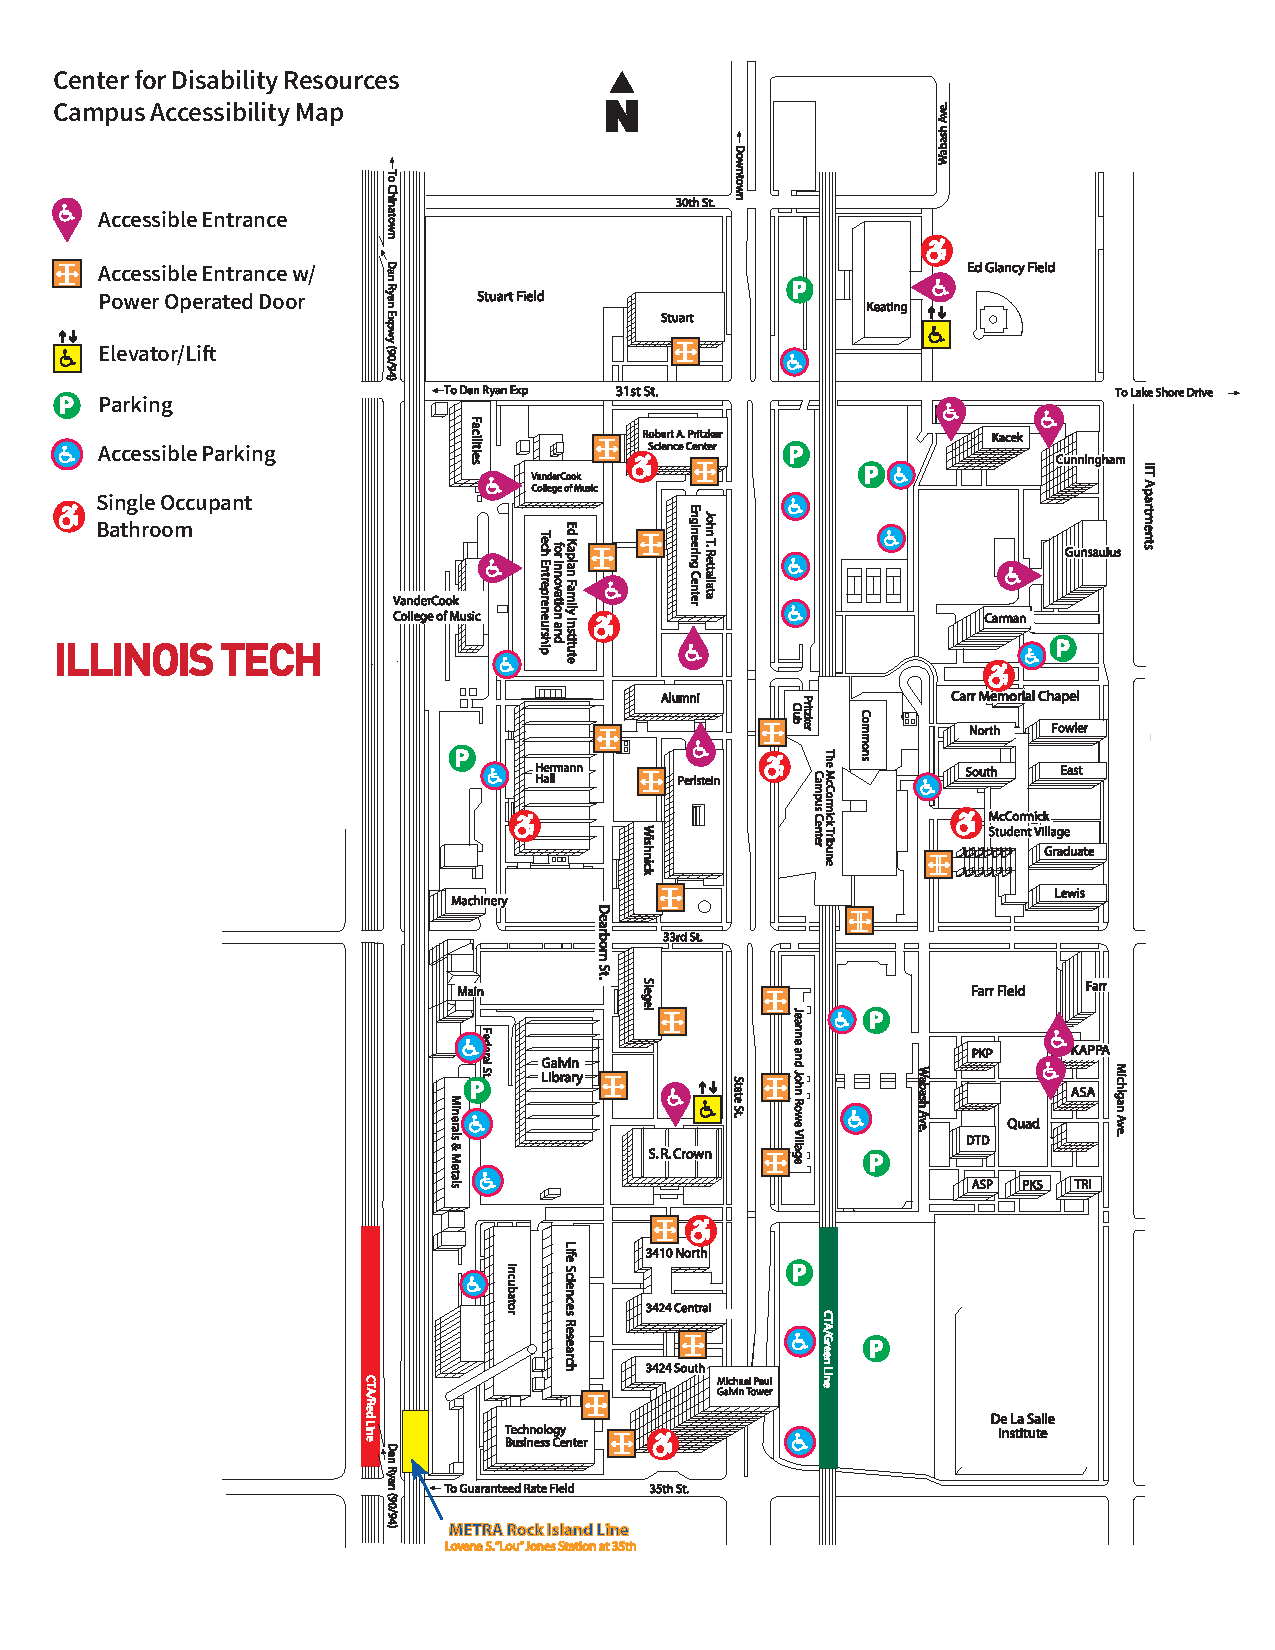
\includegraphics[width = \textwidth] {Photos/mies-campus-accessibility-map-2022.pdf}
\end{center}



\begin{center}
	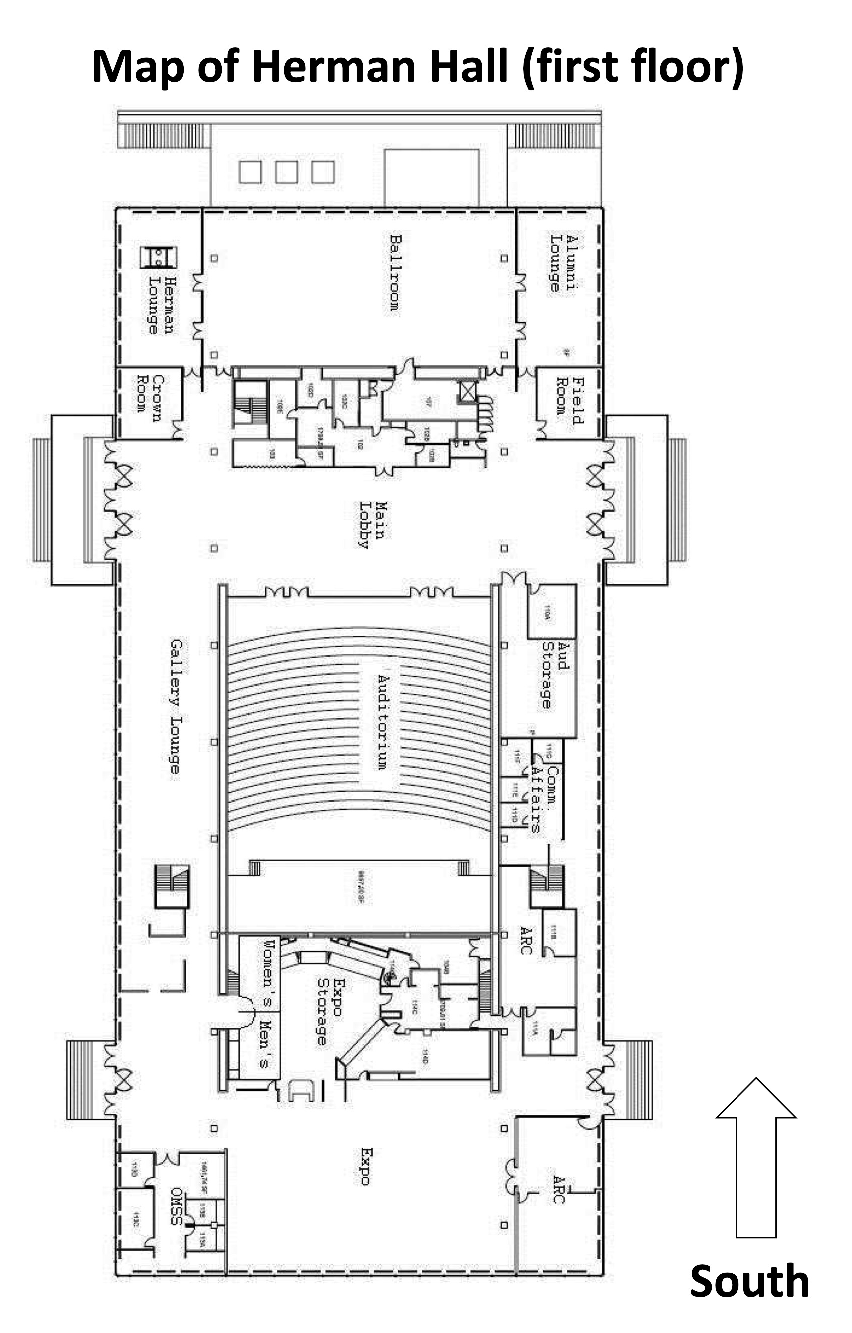
\includegraphics[width =0.95 \textwidth] {Photos/MapHermannHallFirstFloor_cropped.eps}
\end{center}
\clearpage

\section{Getting to Illinois Tech}

\subsection{Local Transportation}
Illinois Tech is located several miles south of downtown.  You  can reach Illinois Tech via 
\begin{itemize}
	\item the Chicago Transit Authority (\href{https://www.transitchicago.com/schedules/}{CTA}) `L' Green or Red Lines, which stop at 35th Street, 
	\item the href{https://www.transitchicago.com/schedules/}{CTA} Route 29 bus, which stops at the corner of State and 32nd Streets, or
	\item taxi, Uber, or Lyft.
	 \item If you are driving to Illinois Tech, there is paid visitor parking in the lot on the east side of State Street between 31st and 32nd Streets (enter via State Street).
\end{itemize}

\subsection{Getting to Chicago}

\begin{itemize}
  \item Two major airports, \href{https://www.flychicago.com/ohare/home/Pages/default.aspx}{O'Hare} and \href{https://www.flychicago.com/midway/pages/default.aspx}{Midway} serve Chicago, and are not far from Illinois Tech.  
  \item Our main domestic passenger rail line is \href{Amtrak}{https://www.amtrak.com/home.html}.
\end{itemize}


\section{Food}

Meals will \emph{not} be provided, except for the Wednesday night conference banquet. There are several places on campus or nearby where you can purchase meals.  They are show in \href{https://www.google.com/maps/d/u/1/edit?mid=1QH5guZDg-m8_f1oO9HgZ5sIL76q1gdk&usp=sharing}{this Google map}


\begin{itemize}
	\item Cafeteria in the McCormick Tribune Conference Center near State and 32nd Street
	\item On 31st Street between Near W
	\begin{itemize}
		\item \href{https://www.yelp.com/biz/yees-cantonese-kitchen-chicago-2?osq=Restaurants} {Yee's Cantonese Kitchen}  
	\end{itemize}
		\item Near the corner of 33rd Street and Wentworth Avenue Streets
	\begin{itemize}
		\item Jimmy John's submarine sandwiches
		\item Starbucks
	\end{itemize}
	
	\item Near the corner of 35th and State Streets
	\begin{itemize}
		\item Jimmy John's submarine sandwiches
		\item Starbucks
	\end{itemize}


\end{itemize}



%\begin{center}
% \includegraphics[width=14cm]{Food_map}
%\end{center}


\section{Technology}

\subsubsection{Equipment in classrooms used for conference}

TBD


\subsubsection{Internet Access}

Illinois Institute of Technology is a partner with eduroam, and you can get internet access via that route if your institution is an eduroam partner.

[IIT guests to be filled in]

\subsubsection{Electrical Power}

In the United States, the standard voltage is 120V at a frequency of 60Hz.  The standard power plugs are 
\begin{itemize}
	\item Type A (two flat parallel pins) and 
	\item Type B (two flat parallel pins plus a round grounding pin).
\end{itemize}

\section{Health and Safety}

\subsection{Nondiscrimination}
This conference adheres to the nondiscrimination policies of the Illinois Institute of Technology (see \href{https://webmaster.iit.edu/files/general-counsel/policies-and-procedures/procedure-p6-non-discrimination-policy.pdf}{\nolinkurl{webmaster.iit.edu/files/general-counsel/policies-and-procedures/procedure-p6-non-discrimination-policy.pdf}}) and also of the University of Chicago (see \href{https://www.uchicago.edu/non-discrimination}{\nolinkurl{www.uchicago.edu/non-discrimination}}), which houses our sponsor the US NSF Institute for Mathematical and Statistical innovation(IMSI).


\subsection{Emergency Contacts, Hospitals and Services on Campus}

TBD



\section{Conference Statistics (as of \today)}

\begin{center}
 \begin{tabular}{ll}
 Number of participants & ?? \\
 Number of plenary lectures & 8 \\
 Number of talks & ?? \\
 Number of special sessions & ?? \\
 Number of technical sessions & ?? \\
 \end{tabular}
\end{center}  % old

%\chapter{List of participants (as of May 14)}

\setlength{\columnsep}{1cm}

\begin{multicols}{2}

\small
\raggedright

\participantne{Ben Adcock}
{ Simon Fraser University }
{SS6-1}
{}
\participantne{Elliot Addy}
{ University of Edinburgh }
{SS18-2}
{}
\participantne{Sanket Agrawal}
{ University of Warwick }
{CS7-2}
{}
\participantne{Miguel Angel Alvarez Ballesteros}
{ King Abdullah University of Science and Technology }
{}
{}
\participantne{Charly Andral}
{ Université Paris Dauphine - PSL }
{CS5-4}
{}
\participantne{Vishnupriya Anupindi}
{ RICAM, Austrian Academy of Sciences }
{CS1-3}
{}
\participantne{Andrea Barth}
{ University of Stuttgart }
{SS19-2}
{}
\participantne{Arved Bartuska}
{ RWTH Aachen University }
{SS13-4}
{}
\participantne{Laura Bazahica}
{ LUT University }
{SS12-3}
{}
\participantne{Ayoub Belhadji}
{ Massachusetts Institute of Technology }
{SS7-1}
{}
\participantne{Cameron Bell}
{ University of Warwick }
{SS1-4}
{}
\participantne{Eya Ben Amar}
{ King Abdullah University of Science and Technology }
{SS20-1}
{}
\participantne{Chiheb Ben Hammouda}
{ Utrecht University }
{SS16-2}
{}
\participantne{Philippe Blondeel}
{ Belgian Royal Military Academy }
{CS5-3}
{}
\participantne{Alexandre Bouchard-Cote}
{ University of British Columbia }
{SS17-2}
{}
\participantne{Ilhem Bouderbala}
{ Unviersity of Alberta }
{CS12-4}
{}
\participantne{Arne Bouillon}
{ KU Leuven }
{CS11-3}
{}
\participantne{Francois-Xavier Briol}
{ University College London }
{SS2-1}
{}
\participantne{Stefano Bruno}
{ University of Edinburgh }
{}
{}
\participantne{Rocco Caprio}
{ University of Warwick }
{CS6-3}
{}
\participantne{Martin Chak}
{ Sorbonne Université }
{}
{}
\participantne{Chuntao Chen}
{ Lappeenranta University of Technology }
{CS11-2}
{}
\participantne{Chek Hin Choi}
{ National University of Singapore }
{SS1-1}
{}
\participantne{Jon Cockayne}
{ University of Southampton }
{SS2-2}
{}
\participantne{Ronald Cools}
{ KU Leuven }
{}
{}
\participantne{Fred Daum}
{ Raytheon }
{}
{}
\participantne{Filippo De Angelis}
{ University of Oxford }
{SS22-2}
{}
\participantne{Gregory de Salaberry Seljak}
{ Universite de Montreal }
{}
{}
\participantne{Josef Dick}
{ UNSW Sydney }
{SS8-1}
{}
\participantne{Jiarui Du}
{ South China University of Technology }
{CS12-2}
{}
\participantne{svetlana Dubinkina}
{ VU Amsterdam }
{SS17-3}
{}
\participantne{Simon Ellinger}
{ University of Passau }
{SS4-3}
{}
\participantne{Ambrose  Emmett-Iwaniw}
{ University of Waterloo }
{CS4-2}
{}
\participantne{Romain Espoeys}
{ CERFACS }
{SS20-3}
{}
\participantne{Ben Feng}
{ University of Waterloo }
{}
{}
\participantne{Damir Ferizović}
{ KU Leuven }
{CS2-1}
{}
\participantne{Jasmin Fiedler}
{ Hochschule Ruhr West }
{}
{}
\participantne{Gersende Fort}
{ CNRS Toulouse }
{PL01}
{}
\participantne{Peter Frazier}
{ Cornell University }
{TUT02}
{}
\participantne{Mike Giles}
{ University of Oxford }
{SS22-3}
{}
\participantne{Michael Gnewuch}
{ Osnabrück University }
{SS24-1}
{}
\participantne{Takashi Goda}
{ University of Tokyo }
{PL02}
{}
\participantne{Ankit Gupta}
{ ETH Zurich }
{SS16-3}
{}
\participantne{Philipp Guth}
{ RICAM }
{SS13-1}
{}
\participantne{Shin Harase}
{ Ritsumeikan University }
{CS12-3}
{}
\participantne{Helmut Harbrecht}
{ University of Basel }
{SS13-2}
{}
\participantne{Zhijian He}
{ South China University of Technology }
{SS14-4}
{}
\participantne{Stefan Heinrich}
{ Rheinland-Pfälzische Technische Universität Kaiserslautern-Landau }
{SS5-1}
{}
\participantne{Astrid Herremans}
{ KU Leuven }
{CS9-1}
{}
\participantne{Fred  Hickernell}
{ Illinois Institute of Technology }
{SS8-2}
{TUT01}
\participantne{Max Hird}
{ University College London }
{CS6-2}
{}
\participantne{Håkon Hoel}
{ University of Oslo }
{SS21-2}
{}
\participantne{Sascha Holl}
{ Max Planck Institute for Informatics }
{}
{}
\participantne{Xun Huan}
{ University of Michigan }
{SS10-2}
{}
\participantne{Anastasia Istratuca}
{ University of Edinburgh }
{SS21-1}
{}
\participantne{Agassi Iu}
{ Wilfrid Laurier University }
{}
{}
\participantne{Thomas Jahn}
{ Catholic University of Eichstätt-Ingolstadt }
{SS7-2}
{}
\participantne{Vesa Kaarnioja}
{ University of Potsdam }
{SS18-4}
{}
\participantne{Miika Kailas}
{ University of Jyväskylä }
{CS7-3}
{}
\participantne{Hye-Won Kang}
{ University of Maryland, Baltimore County }
{SS15-1}
{}
\participantne{Alexander Keller}
{ Nvidia }
{CS8-1}
{}
\participantne{Abdul Khan}
{ Balochistan University of Information Technology }
{}
{}
\participantne{Hwanwoo Kim}
{ Duke University }
{CS6-4}
{}
\participantne{Kristin Kirchner}
{ Delft University of Technology }
{CS3-2}
{}
\participantne{Nathan  Kirk}
{ University of Waterloo }
{CS1-1}
{}
\participantne{Ilja Klebanov}
{ Free University of Berlin }
{SS11-4}
{}
\participantne{David Krieg}
{ JKU Linz }
{PL03}
{}
\participantne{Peter Kritzer}
{ RICAM, Austrian Academy of Sciences }
{CS2-3}
{}
\participantne{Sebastian Krumscheid}
{ Karlsruhe Institute of Technology }
{SS18-1}
{}
\participantne{Sergey Kucherenko}
{ Imperial College London }
{SS14-3}
{}
\participantne{Frances Kuo}
{ UNSW Sydney }
{PL04}
{}
\participantne{Pierre L'Ecuyer}
{ Université de Montréal }
{SS23-2}
{}
\participantne{Henry Lam}
{ Columbia University }
{PL05}
{}
\participantne{Jonas Latz}
{ University of Manchester }
{SS17-1}
{}
\participantne{Christiane Lemieux}
{ University of Waterloo }
{}
{}
\participantne{Matthew Li}
{ Massachusetts Institute of Technology }
{CS8-3}
{}
\participantne{Sifan Liu}
{ Stanford University }
{SS14-2}
{}
\participantne{Emil Løvbak}
{ Karlsruhe Institute of Technology }
{SS21-3}
{}
\participantne{Jun Luo}
{ Shanghai Jiao Tong University }
{}
{}
\participantne{Hassan Maatouk}
{ CY Tech Cergy Paris University }
{CS9-2}
{}
\participantne{Florian Maire}
{ Université de Montréal }
{CS8-2}
{}
\participantne{Josef Martínek}
{ Heidelberg University }
{SS21-4}
{}
\participantne{Michael Mascagni}
{ NIST/Florida State University }
{SS23-1}
{}
\participantne{Alessandro Mastrototaro}
{ KTH Royal Institute of Technology, Stockholm, Sweden }
{CS8-4}
{}
\participantne{Jean de Dieu Mbarushimana}
{ J\&GB SQUARE Ltd }
{}
{}
\participantne{Michael McCourt}
{ Distributional }
{SS9-2}
{}
\participantne{Federica Milinanni}
{ KTH Royal Institute of Technology }
{SS1-2}
{}
\participantne{John Miller}
{ Duke University }
{SS9-3}
{}
\participantne{Weiwen Mo}
{ KU Leuven }
{SS18-3}
{}
\participantne{Hozumi Morohosi}
{ National Graduate Institute for Policy Studies }
{CS1-2}
{}
\participantne{Agnes Mukarugwiro}
{ XXX }
{  }
{}
\participantne{Thomas Müller-Gronbach}
{ University of Passau }
{}
{}
\participantne{Fabio Musco}
{ University of Stuttgart }
{SS13-3}
{}
\participantne{Nicolas Nagel}
{ Chemnitz University of Technology }
{SS5-3}
{}
\participantne{Makoto Narita}
{ National Institute of Technology, Okinawa College }
{}
{}
\participantne{Robert Ndahiro}
{ Nard Ltd }
{}
{}
\participantne{Ning Ning}
{ Texas A\&M University }
{SS1-3}
{}
\participantne{Fabio Nobile}
{ EPFL }
{SS22-1}
{}
\participantne{Dirk Nuyens}
{ KU Leuven }
{SS12-1}
{}
\participantne{Chris Oates}
{ Newcastle University }
{SS11-3}
{PL06}
\participantne{Mariana Olvera-Cravioto}
{ University of North Carolina (Chapel Hill) }
{PL07}
{}
\participantne{Victor Ostromoukhov}
{ Université Claude Bernard Lyon 1 }
{CS1-4}
{}
\participantne{Art Owen}
{ Stanford University }
{PL08}
{}
\participantne{Zexin Pan}
{ Stanford University }
{}
{}
\participantne{Joonha Park}
{ University of Kansas }
{CS12-1}
{}
\participantne{Leszek Plaskota}
{ University of Warsaw, Poland }
{CS4-1}
{}
\participantne{Kateryna Pozharska}
{ Institute of Mathematics of the National Academy of Sciences of Ukraine,  Kyiv, Ukraine / Chemnitz University of Technology, Chemnitz, Germany }
{SS5-2}
{}
\participantne{Vishwas Rao}
{ Argonne National Laboratory }
{SS10-3}
{}
\participantne{Muruhan Rathinam}
{ University of Maryland }
{SS16-1}
{}
\participantne{Christopher Rauhögger}
{ University of Passau }
{SS4-1}
{}
\participantne{Klaus Ritter}
{ RPTU Kaiserslautern }
{SS3-3}
{}
\participantne{Pieterjan Robbe}
{ Sandia National Laboratories }
{SS9-1}
{}
\participantne{Daniel Rudolf}
{ Universität Passau }
{SS3-1}
{}
\participantne{Robin Rüßmann}
{ Rheinland-Pfälzische Technische Universität Kaiserslautern-Landau }
{SS24-3}
{}
\participantne{Asaki Saito}
{ Future University Hakodate }
{SS23-4}
{}
\participantne{Michael Samet}
{ RWTH Aachen University }
{SS14-1}
{}
\participantne{Laura Scarabosio}
{ Radboud University }
{SS19-1}
{}
\participantne{Zheyang Shen}
{ Newcastle University }
{SS2-3}
{}
\participantne{Winfried Sickel}
{ Friedrich-Schiller- University }
{SS6-2}
{}
\participantne{Gurprit Singh}
{ Max Planck Institute for Informatics }
{}
{}
\participantne{Sabrina Sixta}
{ University of Toronto }
{}
{}
\participantne{Ian Sloan}
{ UNSW Sydney }
{SS11-1}
{}
\participantne{Michal Sobieraj}
{ AGH University of Krakow }
{CS3-1}
{}
\participantne{Silei Song}
{ Florida State University }
{CS3-3}
{}
\participantne{Mathias Sonnleitner}
{ University of Münster }
{SS6-3}
{}
\participantne{Aleksei Sorokin}
{ Illinois Institute of Technology }
{SS10-1}
{}
\participantne{Bjoern Sprungk}
{ TU Bergakademie Freiberg }
{CS6-1}
{}
\participantne{Abirami Srikumar}
{ UNSW Sydney }
{SS12-2}
{}
\participantne{Lukasz Stepien}
{ AGH University of Krakow, Poland }
{SS4-2}
{}
\participantne{Shyam Mohan Subbiah Pillai}
{ RWTH Aachen }
{SS20-2}
{}
\participantne{Kosuke Suzuki}
{ Yamagata University }
{SS8-3}
{}
\participantne{Fabian Taubert}
{ University of Technology Chemnitz }
{SS6-4}
{}
\participantne{Aretha Teckentrup}
{ University of Edinburgh }
{SS19-3}
{}
\participantne{Raul Tempone}
{ KAUST }
{}
{}
\participantne{Tino Ullrich}
{ Chemnitz University of Technology }
{SS7-3}
{}
\participantne{Frank Van der Meulen}
{ Vrije Universiteit Amsterdam }
{SS15-3}
{}
\participantne{Xiaoqun Wang}
{ Tsinghua University }
{}
{}
\participantne{Laura Weidensager}
{ TU Chemnitz }
{SS24-2}
{}
\participantne{Christian Weiss}
{ Ruhr West University of Applied Sciences }
{CS2-2}
{}
\participantne{Sophia Wiechert}
{ RWTH Aachen }
{SS15-2}
{}
\participantne{Laurence Wilkes}
{ KU Leuven }
{SS8-4}
{}
\participantne{Leon Wilkosz}
{ KAUST }
{CS5-2}
{}
\participantne{Marcin Wnuk}
{ Osnabrück University }
{SS3-2}
{}
\participantne{Jun Xian}
{ Sun Yat-sen University }
{CS5-1}
{}
\participantne{Yifei Xiong}
{ Pursue University }
{CS4-3}
{}
\participantne{Yunfeng Xiong}
{ Beijing Normal University }
{CS4-3}
{}
\participantne{Xiaoda Xu}
{ Sun Yat-sen University }
{}
{}
\participantne{Jiefei Yang}
{ University of Hong Kong }
{CS7-1}
{}
\participantne{André-Alexander Zepernick}
{ Freie Universität Berlin }
{SS12-4}
{}
\participantne{Yiqing Zhou}
{ KU Leuven }
{}
{}
\participantne{Xiaotian Zhu}
{ Western University }
{CS9-3}
{}

\end{multicols}

 % old
%\chapter{List of Participants (as of May 14)}

\setlength{\columnsep}{1cm}

\begin{multicols}{2}

\small


\participant{Ben Adcock}
{ Simon Fraser University }
{ ben_adcock@sfu.ca }
{SS6-1}
{}
\participant{Elliot Addy}
{ University of Edinburgh }
{ e.j.addy@sms.ed.ac.uk }
{SS18-2}
{}
\participant{Sanket Agrawal}
{ University of Warwick }
{ sanket.agrawal@warwick.ac.uk }
{CS7-2}
{}
\participant{Miguel Angel Alvarez Ballesteros}
{ King Abdullah University of Science and Technology }
{ miguelangel.alvarezballesteros@kaust.edu.sa }
{}
{}
\participant{Charly Andral}
{ Université Paris Dauphine - PSL }
{ andral@ceremade.dauphine.fr }
{CS5-4}
{}
\participant{Vishnupriya Anupindi}
{ RICAM, Austrian Academy of Sciences }
{ vishnupriya.anupindi@ricam.oeaw.ac.at }
{CS1-3}
{}
\participant{Andrea Barth}
{ University of Stuttgart }
{ andrea.barth@mathematik.uni-stuttgart.de }
{SS19-2}
{}
\participant{Arved Bartuska}
{ RWTH Aachen University }
{ arved.bartuska@gmail.com }
{SS13-4}
{}
\participant{Laura Bazahica}
{ LUT University }
{ laura.bazahica@lut.fi }
{SS12-3}
{}
\participant{Ayoub Belhadji}
{ Massachusetts Institute of Technology }
{ abelhadj@mit.edu }
{SS7-1}
{}
\participant{Cameron Bell}
{ University of Warwick }
{ cameron.bell@warwick.ac.uk }
{SS1-4}
{}
\participant{Eya Ben Amar}
{ King Abdullah University of Science and Technology }
{ eya.benamar@kaust.edu.sa }
{SS20-1}
{}
\participant{Chiheb Ben Hammouda}
{ Utrecht University }
{ c.benhammouda@uu.nl }
{SS16-2}
{}
\participant{Philippe Blondeel}
{ Belgian Royal Military Academy }
{ philippe.blondeel@mil.be }
{CS5-3}
{}
\participant{Alexandre Bouchard-Cote}
{ University of British Columbia }
{ bouchard@stat.ubc.ca }
{SS17-2}
{}
\participant{Ilhem Bouderbala}
{ Unviersity of Alberta }
{ bouderba@ualberta.ca }
{CS12-4}
{}
\participant{Arne Bouillon}
{ KU Leuven }
{ arne.bouillon@kuleuven.be }
{CS11-3}
{}
\participant{Francois-Xavier Briol}
{ University College London }
{ f.briol@ucl.ac.uk }
{SS2-1}
{}
\participant{Stefano Bruno}
{ University of Edinburgh }
{ sbruno@ed.ac.uk }
{SS3-1}
{}
\participant{Rocco Caprio}
{ University of Warwick }
{ rocco.caprio@warwick.ac.uk }
{CS6-3}
{}
\participant{Martin Chak}
{ Sorbonne Université }
{ martin.chak@sorbonne-universite.fr }
{}
{}
\participant{Chuntao Chen}
{ Lappeenranta University of Technology }
{ chuntao.chen@lut.fi }
{CS11-2}
{}
\participant{Chek Hin Choi}
{ National University of Singapore }
{ mchchoi@nus.edu.sg }
{SS1-1}
{}
\participant{Jon Cockayne}
{ University of Southampton }
{ jon.cockayne@soton.ac.uk }
{SS2-2}
{}
\participant{Ronald Cools}
{ KU Leuven }
{ ronald.cools@kuleuven.be }
{}
{}
\participant{Fred Daum}
{ Raytheon }
{ daum@raytheon.com }
{}
{}
\participant{Filippo De Angelis}
{ University of Oxford }
{ filippo.deangelis@maths.ox.ac.uk }
{SS22-2}
{}
\participant{Gregory de Salaberry Seljak}
{ Universite de Montreal }
{ gregory.de.salaberry.seljak@umontreal.ca }
{}
{}
\participant{Josef Dick}
{ UNSW Sydney }
{ josef.dick@unsw.edu.au }
{SS8-1}
{}
\participant{Jiarui Du}
{ South China University of Technology }
{ mascut.dujiarui@mail.scut.edu.cn }
{CS12-2}
{}
\participant{svetlana Dubinkina}
{ VU Amsterdam }
{ s.b.dubinkina@vu.nl }
{SS17-3}
{}
\participant{Simon Ellinger}
{ University of Passau }
{ simon.ellinger@uni-passau.de }
{SS4-3}
{}
\participant{Ambrose  Emmett-Iwaniw}
{ University of Waterloo }
{ arsemmettiwaniw@uwaterloo.ca }
{CS4-2}
{}
\participant{Romain Espoeys}
{ CERFACS }
{ espoeys@cerfacs.fr }
{SS20-3}
{}
\participant{Ben Feng}
{ University of Waterloo }
{ ben.feng@uwaterloo.ca }
{}
{}
\participant{Damir Ferizović}
{ KU Leuven }
{ damir.ferizovic@kuleuven.be }
{CS2-4}
{}
\participant{Jasmin Fiedler}
{ Hochschule Ruhr West }
{ jasmin.fiedler@hs-ruhrwest.de }
{}
{}
\participant{Gersende Fort}
{ CNRS Toulouse }
{ gersende.fort@math.univ-toulouse.fr }
{PL01}
{}
\participant{Peter Frazier}
{ Cornell University }
{ pf98@cornell.edu }
{TUT02}
{}
\participant{Mike Giles}
{ University of Oxford }
{ mike.giles@maths.ox.ac.uk }
{SS22-3}
{}
\participant{Michael Gnewuch}
{ Osnabrück University }
{ michael.gnewuch@uos.de }
{SS24-1}
{}
\participant{Takashi Goda}
{ University of Tokyo }
{ goda@frcer.t.u-tokyo.ac.jp }
{PL02}
{}
\participant{Ankit Gupta}
{ ETH Zurich }
{ ankit.gupta@bsse.ethz.ch }
{SS16-3}
{}
\participant{Philipp Guth}
{ RICAM }
{ philipp.guth@ricam.oeaw.ac.at }
{SS13-1}
{}
\participant{Shin Harase}
{ Ritsumeikan University }
{ harase@fc.ritsumei.ac.jp }
{CS12-3}
{}
\participant{Helmut Harbrecht}
{ University of Basel }
{ helmut.harbrecht@unibas.ch }
{SS13-2}
{}
\participant{Zhijian He}
{ South China University of Technology }
{ hezhijian@scut.edu.cn }
{SS14-4}
{}
\participant{Stefan Heinrich}
{ Rheinland-Pfälzische Technische Universität Kaiserslautern-Landau }
{ heinrich@informatik.uni-kl.de }
{SS5-1}
{}
\participant{Astrid Herremans}
{ KU Leuven }
{ astrid.herremans@kuleuven.be }
{CS9-1}
{}
\participant{Fred  Hickernell}
{ Illinois Institute of Technology }
{ hickernell@iit.edu }
{SS8-2}
{TUT01}
\participant{Max Hird}
{ University College London }
{ max.hird.19@ucl.ac.uk }
{CS6-2}
{}
\participant{Håkon Hoel}
{ University of Oslo }
{ haakonah@math.uio.no }
{SS21-2}
{}
\participant{Sascha Holl}
{ Max Planck Institute for Informatics }
{ sholl@mpi-inf.mpg.de }
{CS7-1}
{}
\participant{Xun Huan}
{ University of Michigan }
{ xhuan@umich.edu }
{SS10-2}
{}
\participant{Anastasia Istratuca}
{ University of Edinburgh }
{ a.istratuca@sms.ed.ac.uk }
{SS21-1}
{}
\participant{Agassi Iu}
{ Wilfrid Laurier University }
{ iuxx9590@mylaurier.ca }
{}
{}
\participant{Thomas Jahn}
{ Catholic University of Eichstätt-Ingolstadt }
{ thomas.jahn@ku.de }
{SS7-2}
{}
\participant{Vesa Kaarnioja}
{ University of Potsdam }
{ vesa.kaarnioja@iki.fi }
{SS18-4}
{}
\participant{Miika Kailas}
{ University of Jyväskylä }
{ miika.p.kailas@jyu.fi }
{CS7-3}
{}
\participant{Hye-Won Kang}
{ University of Maryland, Baltimore County }
{ hwkang@umbc.edu }
{SS15-1}
{}
\participant{Alexander Keller}
{ Nvidia }
{ keller.alexander@gmail.com }
{CS8-1}
{}
\participant{Abdul Khan}
{ Balochistan University of Information Technology }
{ qnkhan99@gmail.com }
{}
{}
\participant{Hwanwoo Kim}
{ Duke University }
{ ghksdn1227@gmail.com }
{CS6-4}
{}
\participant{Kristin Kirchner}
{ Delft University of Technology }
{ k.kirchner@tudelft.nl }
{CS3-2}
{}
\participant{Nathan  Kirk}
{ University of Waterloo }
{ n2kirk@uwaterloo.ca }
{CS1-1}
{}
\participant{Ilja Klebanov}
{ Free University of Berlin }
{ klebanov@zedat.fu-berlin.de }
{SS11-4}
{}
\participant{David Krieg}
{ JKU Linz }
{ david.krieg@uni-passau.de }
{PL03}
{}
\participant{Peter Kritzer}
{ RICAM, Austrian Academy of Sciences }
{ peter.kritzer@oeaw.ac.at }
{CS2-3}
{}
\participant{Sebastian Krumscheid}
{ Karlsruhe Institute of Technology }
{ sebastian.krumscheid@kit.edu }
{SS18-1}
{}
\participant{Sergey Kucherenko}
{ Imperial College London }
{ s.kucherenko@imperial.ac.uk }
{SS14-3}
{}
\participant{Frances Kuo}
{ UNSW Sydney }
{ f.kuo@unsw.edu.au }
{PL04}
{}
\participant{Pierre L'Ecuyer}
{ Université de Montréal }
{ lecuyer@iro.umontreal.ca }
{SS23-2}
{}
\participant{Henry Lam}
{ Columbia University }
{ khl2114@columbia.edu }
{PL05}
{}
\participant{Jonas Latz}
{ University of Manchester }
{ jonas.latz@manchester.ac.uk }
{SS17-1}
{}
\participant{Christiane Lemieux}
{ University of Waterloo }
{ clemieux@uwaterloo.ca }
{}
{}
\participant{Matthew Li}
{ Massachusetts Institute of Technology }
{ mtcli@mit.edu }
{CS8-3}
{}
\participant{Sifan Liu}
{ Stanford University }
{ sfliu@stanford.edu }
{SS14-2}
{}
\participant{Emil Løvbak}
{ Karlsruhe Institute of Technology }
{ emil.loevbak@kit.edu }
{SS21-3}
{}
\participant{Jun Luo}
{ Shanghai Jiao Tong University }
{ jluo_ms@sjtu.edu.cn }
{CS10-1}
{}
\participant{Hassan Maatouk}
{ CY Tech Cergy Paris University }
{ maatouk_hassan@hotmail.fr }
{CS9-2}
{}
\participant{Florian Maire}
{ Université de Montréal }
{ florian.maire@umontreal.ca }
{CS8-2}
{}
\participant{Josef Martínek}
{ Heidelberg University }
{ martinek@math.uni-heidelberg.de }
{SS21-4}
{}
\participant{Michael Mascagni}
{ NIST/Florida State University }
{ michael.mascagni@gmail.com }
{SS23-1}
{}
\participant{Alessandro Mastrototaro}
{ KTH Royal Institute of Technology, Stockholm, Sweden }
{ alemas@kth.se }
{CS8-4}
{}
\participant{Jean de Dieu Mbarushimana}
{ J\&GB SQUARE Ltd }
{ jadosxx202@gmail.com }
{}
{}
\participant{Michael McCourt}
{ Distributional }
{ michael@distributional.com }
{SS9-2}
{}
\participant{Federica Milinanni}
{ KTH Royal Institute of Technology }
{ fedmil@kth.se }
{SS1-2}
{}
\participant{John Miller}
{ Duke University }
{ john.joshua.miller@duke.edu }
{SS9-3}
{}
\participant{Weiwen Mo}
{ KU Leuven }
{ weiwen.mo@kuleuven.be }
{SS18-3}
{}
\participant{Hozumi Morohosi}
{ National Graduate Institute for Policy Studies }
{ morohosi@grips.ac.jp }
{CS1-2}
{}
\participant{Agnes Mukarugwiro}
{ XXX }
{ agnesmukarugwiro@gmail.com }
{}
{}
\participant{Thomas Muller-Gronbach}
{ University of Passau }
{ thomas.mueller-gronbach@uni-passau.de }
{}
{}
\participant{Fabio Musco}
{ University of Stuttgart }
{ fabio.musco@mathematik.uni-stuttgart.de }
{SS13-3}
{}
\participant{Nicolas Nagel}
{ Chemnitz University of Technology }
{ nicolas.nagel@mathematik.tu-chemnitz.de }
{SS5-3}
{}
\participant{Makoto Narita}
{ National Institute of Technology, Okinawa College }
{ narita@okinawa-ct.ac.jp }
{}
{}
\participant{Robert Ndahiro}
{ Nard Ltd }
{ ndahirorob@gmail.com }
{}
{}
\participant{Ning Ning}
{ Texas A\&M University }
{ patning@tamu.edu }
{SS1-3}
{}
\participant{Fabio Nobile}
{ EPFL }
{ fabio.nobile@epfl.ch }
{SS22-1}
{}
\participant{Dirk Nuyens}
{ KU Leuven }
{ dirk.nuyens@kuleuven.be }
{SS12-1}
{}
\participant{Chris Oates}
{ Newcastle University }
{ chris.oates@newcastle.ac.uk }
{SS11-3}
{PL06}
\participant{Mariana Olvera-Cravioto}
{ University of North Carolina (Chapel Hill) }
{ molvera@email.unc.edu }
{PL07}
{}
\participant{Victor Ostromoukhov}
{ Université Claude Bernard Lyon 1 }
{ victor.ostromoukhov@liris.cnrs.fr }
{CS1-4}
{}
\participant{Art Owen}
{ Stanford University }
{ owen@stanford.edu }
{PL08}
{}
\participant{Zexin Pan}
{ Stanford University }
{ zep002@stanford.edu }
{}
{}
\participant{Joonha Park}
{ University of Kansas }
{ j.park@ku.edu }
{CS12-1}
{}
\participant{Leszek Plaskota}
{ University of Warsaw, Poland }
{ leszekp@mimuw.edu.pl }
{CS4-1}
{}
\participant{Kateryna Pozharska}
{ Institute of Mathematics of the National Academy of Sciences of Ukraine,  Kyiv, Ukraine / Chemnitz University of Technology, Chemnitz, Germany }
{ pozharska.k@gmail.com }
{SS5-2}
{}
\participant{Vishwas Rao}
{ Argonne National Laboratory }
{ vhebbur@anl.gov }
{SS10-3}
{}
\participant{Muruhan Rathinam}
{ University of Maryland }
{ muruhan@umbc.edu }
{SS16-1}
{}
\participant{Christopher Rauhögger}
{ University of Passau }
{ rauhoe01@ads.uni-passau.de }
{SS4-1}
{}
\participant{Klaus Ritter}
{ RPTU Kaiserslautern }
{ ritter@mathematik.uni-kl.de }
{SS3-3}
{}
\participant{Pieterjan Robbe}
{ Sandia National Laboratories }
{ pmrobbe@sandia.gov }
{SS9-1}
{}
\participant{Daniel Rudolf}
{ Universität Passau }
{ daniel.rudolf@uni-passau.de }
{SS5-4}
{}
\participant{Robin Rüßmann}
{ Rheinland-Pfälzische Technische Universität Kaiserslautern-Landau }
{ ruessman@mathematik.uni-kl.de }
{SS24-3}
{}
\participant{Asaki Saito}
{ Future University Hakodate }
{ saito@fun.ac.jp }
{SS23-4}
{}
\participant{Michael Samet}
{ RWTH Aachen University }
{ samet@uq.rwth-aachen.de }
{SS14-1}
{}
\participant{Laura Scarabosio}
{ Radboud University }
{ l.scarabosio@math.ru.nl }
{SS19-1}
{}
\participant{Zheyang Shen}
{ Newcastle University }
{ zheyang.shen@newcastle.ac.uk }
{SS2-3}
{}
\participant{Winfried Sickel}
{ Friedrich-Schiller- University }
{ winfried.sickel@uni-jena.de }
{SS6-2}
{}
\participant{Gurprit Singh}
{ Max Planck Institute for Informatics }
{ gsingh@mpi-inf.mpg.de }
{}
{}
\participant{Sabrina Sixta}
{ University of Toronto }
{ sabrina.sixta@mail.utoronto.ca }
{}
{}
\participant{Ian Sloan}
{ UNSW Sydney }
{ i.sloan@unsw.edu.au }
{SS11-1}
{}
\participant{Michal Sobieraj}
{ AGH University of Krakow }
{ sobieraj@agh.edu.pl }
{CS3-1}
{}
\participant{Silei Song}
{ Florida State University }
{ ss19cu@fsu.edu }
{CS3-3}
{}
\participant{Mathias Sonnleitner}
{ University of Münster }
{ math.s@posteo.net }
{SS6-3}
{}
\participant{Aleksei Sorokin}
{ Illinois Institute of Technology }
{ asorokin@hawk.iit.edu }
{SS10-1}
{}
\participant{Bjoern Sprungk}
{ TU Bergakademie Freiberg }
{ bjoern.sprungk@math.tu-freiberg.de }
{CS6-1}
{}
\participant{Abirami Srikumar}
{ UNSW Sydney }
{ a.srikumar@unsw.edu.au }
{SS12-2}
{}
\participant{Lukasz Stepien}
{ AGH University of Krakow, Poland }
{ lstepie@agh.edu.pl }
{SS4-2}
{}
\participant{Shyam Mohan Subbiah Pillai}
{ RWTH Aachen }
{ subbiah@uq.rwth-aachen.de }
{SS20-2}
{}
\participant{Kosuke Suzuki}
{ Yamagata University }
{ kosuke-suzuki@sci.kj.yamagata-u.ac.jp }
{SS8-3}
{}
\participant{Fabian Taubert}
{ University of Technology Chemnitz }
{ fabian.taubert@math.tu-chemnitz.de }
{SS6-4}
{}
\participant{Aretha Teckentrup}
{ University of Edinburgh }
{ a.teckentrup@ed.ac.uk }
{SS19-3}
{}
\participant{Raul Tempone}
{ KAUST }
{ raul.tempone@kaust.edu.sa }
{}
{}
\participant{Tino Ullrich}
{ Chemnitz University of Technology }
{ tino.ullrich@math.tu-chemnitz.de }
{SS7-3}
{}
\participant{Frank Van der Meulen}
{ Vrije Universiteit Amsterdam }
{ f.h.van.der.meulen@vu.nl }
{SS15-3}
{}
\participant{Xiaoqun Wang}
{ Tsinghua University }
{ wangxiaoqun@mail.tsinghua.edu.cn }
{CS2-1}
{}
\participant{Laura Weidensager}
{ TU Chemnitz }
{ laura.weidensager@math.tu-chemnitz.de }
{SS24-2}
{}
\participant{Christian Weiss}
{ Ruhr West University of Applied Sciences }
{ christian.weiss@hs-ruhrwest.de }
{CS2-2}
{}
\participant{Sophia Wiechert}
{ RWTH Aachen }
{ wiechert@uq.rwth-aachen.de }
{SS15-2}
{}
\participant{Laurence Wilkes}
{ KU Leuven }
{ laurence.wilkes@kuleuven.be }
{SS8-4}
{}
\participant{Leon Wilkosz}
{ KAUST }
{ leon.wilkosz@kaust.edu.sa }
{CS5-2}
{}
\participant{Marcin Wnuk}
{ Osnabrück University }
{ marcin.wnuk@uni-osnabrueck.de }
{SS17-4}
{}
\participant{Jun Xian}
{ Sun Yat-sen University }
{ xianjun@mail.sysu.edu.cn }
{CS5-1}
{}
\participant{Jun Xian}
{ Sun Yat-sen University }
{ xianjun@mail.sysu.edu.cn }
{CS5-1}
{}
\participant{Yifei Xiong}
{ Pursue University }
{ xiong173@purdue.edu }
{CS4-3}
{}
\participant{Yunfeng Xiong}
{ Beijing Normal University }
{ yfxiong@bnu.edu.cn }
{CS4-3}
{}
\participant{Jiefei Yang}
{ University of Hong Kong }
{ jiefeiy@connect.hku.hk }
{CS10-2}
{}
\participant{André-Alexander Zepernick}
{ Freie Universität Berlin }
{ a.zepernick@fu-berlin.de }
{SS12-4}
{}
\participant{Yiqing Zhou}
{ KU Leuven }
{ yiqing.zhou@kuleuven.be }
{}
{}
\participant{Xiaotian Zhu}
{ Western University }
{ xzhu444@uwo.ca }
{CS10-3}
{}

\end{multicols}

 % old
\chapter{List of Participants}

\setlength{\columnsep}{1cm}

\begin{multicols}{2}

\small\raggedright

\participantne{Kazeem Adeleke}
{University of the West of England}
{T16-1}
{}
{}
{}
{}
{}
{}
\participantne{Alen Alexanderian}
{North Carolina State University}
{S13}
{}
{}
{}
{}
{}
{}
\participantne{Miguel Alvarez}
{King Abdullah University of Science and Technology}
{T12-2}
{}
{}
{}
{}
{}
{}
\participantne{Nicole Aretz}
{University of Texas at Austin}
{T15-4}
{}
{}
{}
{}
{}
{}
\participantne{Matyokub Bakoev}
{MGIMO, Tashkent}
{T8-1}
{}
{}
{}
{}
{}
{}
\participantne{Krishnakumar Balasubramanian}
{University of California, Davis}
{S23}
{}
{}
{}
{}
{}
{}
\participantne{Nikhil Bansal}
{University of Michigan, Ann Arbor}
{S11}
{}
{}
{}
{}
{}
{}
\participantne{Felix Bartel}
{University of New South Wales}
{S22}
{}
{}
{}
{}
{}
{}
\participantne{Arved Bartuska}
{King Abdullah University of Science and Technology/RWTH Aachen University}
{S3}
{S24}
{}
{}
{}
{}
{}
\participantne{Arved Bartuska}
{RWTH Aachen University}
{S6}
{}
{}
{}
{}
{}
{}
\participantne{Niklas Baumgarten}
{University of Heidelberg}
{S29}
{}
{}
{}
{}
{}
{}
\participantne{Ayoub Belhadji}
{Massachusetts Institute of Technology}
{S9}
{}
{}
{}
{}
{}
{}
\participantne{Eya Ben Amar}
{King Abdullah University of Science and Technology}
{S14}
{}
{}
{}
{}
{}
{}
\participantne{Jose Blanchet}
{Stanford University}
{S27}
{}
{}
{}
{}
{}
{}
\participantne{Frédéric Blondeel}
{Kuleuven and Unife}
{T13-1}
{}
{}
{}
{}
{}
{}
\participantne{Philippe Blondeel}
{Belgian Military Academy}
{T15-1}
{}
{}
{}
{}
{}
{}
\participantne{Andrews Boahen}
{Michigan State University}
{S17}
{}
{}
{}
{}
{}
{}
\participantne{Raghu Bollapragada}
{University of Texas at Austin}
{S19}
{}
{}
{}
{}
{}
{}
\participantne{Nawaf Bou-Rabee}
{Rutgers University}
{S18}
{}
{}
{}
{}
{}
{}
\participantne{Arne Bouillon}
{KU Leuven}
{T6-3}
{}
{}
{}
{}
{}
{}
\participantne{Nicola Branchini}
{University of Edinburgh}
{T9-1}
{}
{}
{}
{}
{}
{}
\participantne{Mou Cai}
{University of Tokyo}
{S22}
{}
{}
{}
{}
{}
{}
\participantne{Wei Cai}
{Southern Methodist University}
{T13-3}
{}
{}
{}
{}
{}
{}
\participantne{Trevor Campbell}
{University of British Columbia}
{S18}
{}
{}
{}
{}
{}
{}
\participantne{Bob Carpenter}
{Flatiron Institute}
{S18}
{}
{}
{}
{}
{}
{}
\participantne{Annabelle Carrell}
{University of Cambridge}
{T14-3}
{}
{}
{}
{}
{}
{}
\participantne{Tommie Catanach}
{Sandia National Laboratories}
{S13}
{}
{}
{}
{}
{}
{}
\participantne{Makram Chahine}
{Massachusetts Institute of Technology}
{S7}
{}
{}
{}
{}
{}
{}
\participantne{Jean-Francois Chassagneux}
{ENSAE Paris}
{S8}
{}
{}
{}
{}
{}
{}
\participantne{Yifan Chen}
{New York University}
{S23}
{S26}
{}
{}
{}
{}
{}
\participantne{Xiaoou Cheng}
{New York University}
{S23}
{S26}
{}
{}
{}
{}
{}
\participantne{Hongmei Chi}
{Florida Aandm University}
{}
{}
{}
{}
{}
{}
{}
\participantne{Sou-Cheng Choi}
{Illinois Institute of Technology}
{S11}
{S15}
{S4}
{S29}
{}
{}
{}
\participantne{Nicolas Chopin}
{ENSAE, Institut Polytechnique de Paris}
{P7}
{}
{}
{}
{}
{}
{}
\participantne{Maksim Chupin}
{King Abdullah University of Science and Technology}
{S28}
{}
{}
{}
{}
{}
{}
\participantne{François Clément}
{University of Washington}
{S7}
{}
{}
{}
{}
{}
{}
\participantne{Reuben Cohn-Gordon}
{University of California, Berkeley}
{T14-1}
{}
{}
{}
{}
{}
{}
\participantne{Adrien Corenflos}
{University of Warwick}
{S9}
{}
{}
{}
{}
{}
{}
\participantne{Steven Damelin}
{Zbmath Open, European Mathematical Society}
{S9}
{}
{}
{}
{}
{}
{}
\participantne{Arghya Datta}
{Université de Montréal}
{T2-3}
{}
{}
{}
{}
{}
{}
\participantne{Jakob Dilen}
{KU Leuven}
{T5-3}
{}
{}
{}
{}
{}
{}
\participantne{Yuhan Ding}
{Illinois Institute of Technology}
{S11}
{S15}
{}
{}
{}
{}
{}
\participantne{Carles Domingo-Enrich}
{Microsoft Research New England}
{T16-2}
{}
{}
{}
{}
{}
{}
\participantne{Jing Dong}
{Columbia University}
{S27}
{}
{}
{}
{}
{}
{}
\participantne{Goncalo Dos~Reis}
{University of Edinburgh}
{S8}
{}
{}
{}
{}
{}
{}
\participantne{Christopher Draper}
{Florida State University}
{T16-3}
{}
{}
{}
{}
{}
{}
\participantne{Jürgen Dölz}
{University of Bonn}
{S2}
{}
{}
{}
{}
{}
{}
\participantne{Victor Elvira}
{University of Edinburgh}
{S14}
{}
{}
{}
{}
{}
{}
\participantne{Ambrose Emmett-Iwaniw}
{University of Waterloo}
{T4-3}
{}
{}
{}
{}
{}
{}
\participantne{Murat Erdogdu}
{University of Toronto}
{S10}
{}
{}
{}
{}
{}
{}
\participantne{Arash Fahim}
{Florida State University}
{S21}
{}
{}
{}
{}
{}
{}
\participantne{Zhou Fang}
{Chinese Academy of Sciences}
{S28}
{}
{}
{}
{}
{}
{}
\participantne{Joseph Farmer}
{University of Notre Dame}
{S29}
{}
{}
{}
{}
{}
{}
\participantne{Serena Fattori}
{Istituto Nazionale di Fisica Nucleare (INFN)}
{T3-2}
{}
{}
{}
{}
{}
{}
\participantne{Florence Forbes}
{Inria}
{S9}
{S13}
{}
{}
{}
{}
{}
\participantne{Noufel Frikha}
{Paris 1 Pantheon-Sorbonne University}
{S8}
{}
{}
{}
{}
{}
{}
\participantne{Noufel Frikha}
{Université Paris 1 Panthéon Sorbonne}
{T12-4}
{}
{}
{}
{}
{}
{}
\participantne{Philippe Gagnon}
{Université de Montréal}
{T1-3}
{}
{}
{}
{}
{}
{}
\participantne{Soumyadip Ghosh}
{IBM Research}
{T7-4}
{}
{}
{}
{}
{}
{}
\participantne{Mike Giles}
{University of Oxford}
{S4}
{S29}
{}
{}
{}
{}
{}
\participantne{Peter Glynn}
{Stanford University}
{P3}
{}
{}
{}
{}
{}
{}
\participantne{Michael Gnewuch}
{University of Osnabrück}
{S22}
{S25}
{}
{}
{}
{}
{}
\participantne{Michael Gnewuch}
{Osnabruck University}
{S5}
{}
{}
{}
{}
{}
{}
\participantne{Takashi Goda}
{University of Tokyo}
{S22}
{S25}
{S15}
{}
{}
{}
{}
\participantne{Sebastiano Grazzi}
{Bocconi University}
{S10}
{}
{}
{}
{}
{}
{}
\participantne{Philipp Guth}
{Austrian Academy of Sciences}
{S2}
{}
{}
{}
{}
{}
{}
\participantne{Philipp Guth}
{Johann Radon Institute for Computational and Applied Mathematics}
{S24}
{}
{}
{}
{}
{}
{}
\participantne{Philipp A. Guth}
{Austrian Academy of Sciences}
{S6}
{}
{}
{}
{}
{}
{}
\participantne{Irina-Beatrice Haas}
{University of Oxford}
{S4}
{}
{}
{}
{}
{}
{}
\participantne{Harri Hakula}
{Aalto University}
{S2}
{}
{}
{}
{}
{}
{}
\participantne{Claude Hall}
{Illinois Institute of Technology}
{T4-4}
{}
{}
{}
{}
{}
{}
\participantne{Chiheb Ben Hammouda}
{Utrecht University}
{S28}
{}
{}
{}
{}
{}
{}
\participantne{Zhijian He}
{South China University of Technology}
{S22}
{}
{}
{}
{}
{}
{}
\participantne{Stefan Heinrich}
{RPTU Kaiserslautern-Landau}
{S1}
{S5}
{S8}
{S12}
{S16}
{}
{}
\participantne{Tapio Helin}
{LUT University}
{S6}
{}
{}
{}
{}
{}
{}
\participantne{Shane Henderson}
{Cornell University}
{S19}
{}
{}
{}
{}
{}
{}
\participantne{Fred Hickernell}
{Illinois Institute of Technology}
{S12}
{}
{}
{}
{}
{}
{}
\participantne{Truong Vinh Hoang}
{RWTH Aachen University}
{S3}
{}
{}
{}
{}
{}
{}
\participantne{Håkon Hoel}
{University of Oslo}
{T12-3}
{}
{}
{}
{}
{}
{}
\participantne{Sascha Holl}
{Max Planck Institute for Informatics}
{T7-2}
{}
{}
{}
{}
{}
{}
\participantne{Xun Huan}
{University of Michigan}
{S9}
{S13}
{}
{}
{}
{}
{}
\participantne{Chaofan Huang}
{Georgia Institute of Technology}
{S17}
{}
{}
{}
{}
{}
{}
\participantne{Chi-Ok Hwang}
{Gwangju Institute of Science and Technology}
{T3-4}
{}
{}
{}
{}
{}
{}
\participantne{Toon Ingelaere}
{KU Leuven}
{T9-3}
{}
{}
{}
{}
{}
{}
\participantne{Jacopo Iollo}
{Inria}
{S13}
{}
{}
{}
{}
{}
{}
\participantne{Joshua Isaacson}
{Fermilab}
{S15}
{}
{}
{}
{}
{}
{}
\participantne{Aadit Jain}
{Rancho Bernardo High School}
{T5-4}
{}
{}
{}
{}
{}
{}
\participantne{Sharanya Jayaraman}
{Florida State University}
{S21}
{}
{}
{}
{}
{}
{}
\participantne{Carlos Jerez-Hanckes}
{Universidad Adolfo Ibáñez}
{S2}
{}
{}
{}
{}
{}
{}
\participantne{Haotian Jiang}
{University of Chicago}
{S20}
{}
{}
{}
{}
{}
{}
\participantne{Roshan Joseph}
{Georgia Institute of Technology}
{P4}
{}
{}
{}
{}
{}
{}
\participantne{Vesa Kaarnioja}
{Free University of Berlin}
{S6}
{S2}
{S3}
{}
{}
{}
{}
\participantne{Lulu Kang}
{University of Massachusetts Amherst}
{S17}
{}
{}
{}
{}
{}
{}
\participantne{Toni Karvonen}
{LUT University}
{}
{}
{}
{}
{}
{}
{}
\participantne{Hwanwoo Kim}
{Duke University}
{S11}
{}
{}
{}
{}
{}
{}
\participantne{Nathan Kirk}
{Illinois Institute of Technology}
{S7}
{}
{}
{}
{}
{}
{}
\participantne{Karina Koval}
{University of Heidelberg}
{S6}
{}
{}
{}
{}
{}
{}
\participantne{Peter Kritzer}
{Austrian Academy of Sciences}
{S22}
{S25}
{T5-1}
{}
{}
{}
{}
\participantne{Johannes Krotz}
{University of Notre Dame}
{S29}
{}
{}
{}
{}
{}
{}
\participantne{Sebastian Krumscheid}
{Karlsruhe Institute of Technology}
{S3}
{}
{}
{}
{}
{}
{}
\participantne{Yashveer Kumar}
{INESC-ID}
{T3-1}
{}
{}
{}
{}
{}
{}
\participantne{Frances Y. Kuo}
{University of New South Wales}
{S22}
{}
{}
{}
{}
{}
{}
\participantne{Kun-Lin Kuo}
{National University of Kaohsiung}
{T7-1}
{}
{}
{}
{}
{}
{}
\participantne{Bernd Käßemodel}
{Chemnitz University of Technology}
{S16}
{}
{}
{}
{}
{}
{}
\participantne{Jimmy Lederman}
{University of Chicago}
{T2-4}
{}
{}
{}
{}
{}
{}
\participantne{Christiane Lemieux}
{University of Waterloo}
{P2}
{}
{}
{}
{}
{}
{}
\participantne{Gunther Leobacher}
{University of Graz}
{S12}
{}
{}
{}
{}
{}
{}
\participantne{Chunfang Lin}
{Queen's University}
{S17}
{}
{}
{}
{}
{}
{}
\participantne{Sifan Liu}
{Flatiron Institute}
{T4-2}
{}
{}
{}
{}
{}
{}
\participantne{Yang Liu}
{King Abdullah University of Science and Technology}
{T5-2}
{}
{}
{}
{}
{}
{}
\participantne{Chung Ming Loi}
{Durham University}
{S4}
{}
{}
{}
{}
{}
{}
\participantne{Attila Lovas}
{Hun-Ren Alfréd Rényi Institute of Mathematics}
{S27}
{}
{}
{}
{}
{}
{}
\participantne{Iosif Lytras}
{Athena/archimedes Research Centre, Greece}
{S16}
{}
{}
{}
{}
{}
{}
\participantne{Simon Mak}
{Duke University}
{S17}
{}
{}
{}
{}
{}
{}
\participantne{Nikolaos Makras}
{University of Edinburgh}
{S16}
{}
{}
{}
{}
{}
{}
\participantne{Youssef Marzouk}
{Massachusetts Institute of Technology}
{S9}
{S13}
{}
{}
{}
{}
{}
\participantne{Michael Mascagni}
{Florida State University and National Institute of Standards and Technology}
{S21}
{}
{}
{}
{}
{}
{}
\participantne{Michael Mascagni}
{Florida State University}
{S11}
{}
{}
{}
{}
{}
{}
\participantne{Larysa Matiukha}
{Illinois Institute of Technology}
{S5}
{}
{}
{}
{}
{}
{}
\participantne{Federica Milinanni}
{KTH Royal Institute of Technology}
{S10}
{}
{}
{}
{}
{}
{}
\participantne{Johannes Milz}
{Georgia Institute of Technology}
{S6}
{}
{}
{}
{}
{}
{}
\participantne{Siddharth Mitra}
{Yale University}
{S26}
{}
{}
{}
{}
{}
{}
\participantne{Chirag Modi}
{New York University}
{S18}
{}
{}
{}
{}
{}
{}
\participantne{Thomas Muller-Gronbach}
{University of Passau}
{S1}
{S5}
{S8}
{S12}
{S16}
{}
{}
\participantne{Sophia Münker}
{RWTH Aachen University}
{S28}
{}
{}
{}
{}
{}
{}
\participantne{Lorenzo Nagar}
{Basque Center for Applied Mathematics}
{T2-1}
{}
{}
{}
{}
{}
{}
\participantne{Andreas Neuenkirch}
{University of Mannheim}
{S1}
{}
{}
{}
{}
{}
{}
\participantne{Aleksandar Nikolov}
{University of Toronto}
{S20}
{}
{}
{}
{}
{}
{}
\participantne{Ziang Niu}
{University of Pennsylvania}
{S15}
{}
{}
{}
{}
{}
{}
\participantne{Muhammad Noor ul Amin}
{COMSATS University Islamabad, Lahore}
{T3-3}
{}
{}
{}
{}
{}
{}
\participantne{Dirk Nuyens}
{KU Leuven}
{S25}
{}
{}
{}
{}
{}
{}
\participantne{Du Ouyang}
{Tsinghua University}
{T13-2}
{}
{}
{}
{}
{}
{}
\participantne{Art Owen}
{Stanford University}
{S18}
{}
{}
{}
{}
{}
{}
\participantne{Art B. Owen}
{Stanford University}
{S25}
{}
{}
{}
{}
{}
{}
\participantne{Zexin Pan}
{Austrian Academy of Sciences}
{S25}
{}
{}
{}
{}
{}
{}
\participantne{Joonha Park}
{University of Kansas}
{T6-2}
{}
{}
{}
{}
{}
{}
\participantne{Raghu Pasupathy}
{Purdue University}
{S19}
{}
{}
{}
{}
{}
{}
\participantne{Rino Persiani}
{INFN Catania}
{T15-2}
{}
{}
{}
{}
{}
{}
\participantne{Shyam Mohan Subbiah Pillai}
{RWTH Aachen University}
{S14}
{}
{}
{}
{}
{}
{}
\participantne{Leszek Plaskota}
{University of Warsaw}
{S5}
{}
{}
{}
{}
{}
{}
\participantne{Kateryna Pozharska}
{Chemnitz University of Technology}
{S5}
{}
{}
{}
{}
{}
{}
\participantne{Sara Pérez-Vieites}
{Aalto University}
{S24}
{}
{}
{}
{}
{}
{}
\participantne{Hao Quan}
{University of Waterloo}
{T8-4}
{}
{}
{}
{}
{}
{}
\participantne{Nadhir Ben Rached}
{University of Leeds}
{S14}
{}
{}
{}
{}
{}
{}
\participantne{Abdujabar Rasulov}
{University of World Economy and Diplomacy}
{T12-1}
{}
{}
{}
{}
{}
{}
\participantne{Muruhan Rathinam}
{University of Maryland, Baltimore}
{S28}
{}
{}
{}
{}
{}
{}
\participantne{Christopher Rauhögger}
{University of Passau}
{S1}
{}
{}
{}
{}
{}
{}
\participantne{Matteo Raviola}
{École Polytechnique Fédérale de Lausanne}
{S24}
{}
{}
{}
{}
{}
{}
\participantne{Chang-Han Rhee}
{Northwestern University}
{S27}
{}
{}
{}
{}
{}
{}
\participantne{Adrien Richou}
{Université de Bordeaux}
{T11-2}
{}
{}
{}
{}
{}
{}
\participantne{Pieterjan Robbe}
{Sandia National Laboratories}
{S4}
{S29}
{}
{}
{}
{}
{}
\participantne{Veronika Ročková}
{University of Chicago}
{P8}
{}
{}
{}
{}
{}
{}
\participantne{Hamza Ruzayqat}
{King Abdullah University of Science and Technology}
{T2-2}
{}
{}
{}
{}
{}
{}
\participantne{Sotirios Sabanis}
{University of Edinburgh}
{S8}
{}
{}
{}
{}
{}
{}
\participantne{Riccardo Saporiti}
{EPFL}
{T11-4}
{}
{}
{}
{}
{}
{}
\participantne{Rohan Sawahney}
{Nvidia Corporation}
{S21}
{}
{}
{}
{}
{}
{}
\participantne{Philip Schaer}
{Friedrich Schiller University Jena}
{T14-2}
{}
{}
{}
{}
{}
{}
\participantne{Verena Schwarz}
{University of Klagenfurt}
{S1}
{}
{}
{}
{}
{}
{}
\participantne{Gregory Seljak}
{University of Montréal}
{S7}
{}
{}
{}
{}
{}
{}
\participantne{Uros Seljak}
{University of California, Berkeley}
{P6}
{}
{}
{}
{}
{}
{}
\participantne{Ruben Seyer}
{Chalmers University of Technology and University of Gothenburg}
{T1-2}
{}
{}
{}
{}
{}
{}
\participantne{Akash Sharma}
{Chalmers Institute of Technology}
{T6-1}
{}
{}
{}
{}
{}
{}
\participantne{Alex Shestopaloff}
{Queen Mary University of London}
{S10}
{}
{}
{}
{}
{}
{}
\participantne{Alex Shkolnik}
{University of California, Santa Barbara}
{T6-4}
{}
{}
{}
{}
{}
{}
\participantne{Prasanth Shyamsundar}
{Fermi National Accelerator Laboratory}
{T15-3}
{}
{}
{}
{}
{}
{}
\participantne{Silei Song}
{Florida State University}
{S21}
{}
{}
{}
{}
{}
{}
\participantne{Aleksei Sorokin}
{Illinois Institute of Technology}
{S29}
{}
{}
{}
{}
{}
{}
\participantne{Alexander Steinicke}
{Technical University of Leoben}
{S12}
{}
{}
{}
{}
{}
{}
\participantne{Shyam Mohan Subbiah Pillai}
{RWTH Aachen University}
{S14}
{}
{}
{}
{}
{}
{}
\participantne{Amit Subrahmanya}
{Virginia Tech}
{T9-4}
{}
{}
{}
{}
{}
{}
\participantne{Kosuke Suzuki}
{Yamagata University}
{S25}
{}
{}
{}
{}
{}
{}
\participantne{Michaela Szölgyenyi}
{University of Klagenfurt}
{P5}
{}
{}
{}
{}
{}
{}
\participantne{Molei Tao}
{Georgia Institute of Technology}
{S26}
{}
{}
{}
{}
{}
{}
\participantne{Raul Tempone}
{RWTH Aachen University}
{S28}
{}
{}
{}
{}
{}
{}
\participantne{Raúl Tempone}
{King Abdullah University of Science and Technology/RWTH Aachen University}
{S3}
{S24}
{}
{}
{}
{}
{}
\participantne{Raúl Tempone}
{King Abdullah University of Science and Technology}
{S14}
{}
{}
{}
{}
{}
{}
\participantne{Bruno Tuffin}
{Inria}
{S14}
{}
{}
{}
{}
{}
{}
\participantne{Lihan Wang}
{Carnegie Mellon University}
{S23}
{}
{}
{}
{}
{}
{}
\participantne{Xingyu Wang}
{University of Amsterdam}
{S10}
{}
{}
{}
{}
{}
{}
\participantne{Zhihao Wang}
{University of Copenhagen}
{T1-1}
{}
{}
{}
{}
{}
{}
\participantne{Jonathan Weare}
{New York University}
{S23}
{S26}
{S11}
{}
{}
{}
{}
\participantne{Christian Weiss}
{Ruhr West University of Applied Sciences}
{T4-1}
{}
{}
{}
{}
{}
{}
\participantne{Josephine Westermann}
{Heidelberg University}
{T7-3}
{}
{}
{}
{}
{}
{}
\participantne{Peter Whalley}
{ETH Zurich}
{S23}
{}
{}
{}
{}
{}
{}
\participantne{Anke Wiese}
{Heriot-Watt University}
{T11-3}
{}
{}
{}
{}
{}
{}
\participantne{Leon Wilkosz}
{King Abdullah University of Science and Technology}
{T8-2}
{}
{}
{}
{}
{}
{}
\participantne{Qian Xiao}
{Shanghai Jiao Tong University}
{S17}
{}
{}
{}
{}
{}
{}
\participantne{Yiming Xu}
{University of Kentucky}
{T16-4}
{}
{}
{}
{}
{}
{}
\participantne{Jun Yang}
{University of Copenhagen}
{S10}
{}
{}
{}
{}
{}
{}
\participantne{Larisa Yaroslavtseva}
{University of Graz}
{S1}
{S5}
{S8}
{S12}
{S16}
{}
{}
\participantne{Daniel Yukimura}
{Impa, Rio de Janeiro}
{T9-2}
{}
{}
{}
{}
{}
{}
\participantne{André-Alexander Zepernick}
{Free University of Berlin}
{S2}
{}
{}
{}
{}
{}
{}
\participantne{Peng Zhang}
{Rutgers University}
{S20}
{}
{}
{}
{}
{}
{}
\participantne{Vincent Zhang}
{University of Southern California}
{T8-3}
{}
{}
{}
{}
{}
{}
\participantne{Chenyang Zhong}
{Columbia University}
{S15}
{}
{}
{}
{}
{}
{}
\participantne{Fuzhong Zhou}
{Columbia University}
{S26}
{}
{}
{}
{}
{}
{}
\participantne{Yiqing Zhou}
{KU Leuven}
{T13-4}
{}
{}
{}
{}
{}
{}
\participantne{Fabio Zoccolan}
{EPFL}
{T11-1}
{}
{}
{}
{}
{}
{}
\end{multicols}

 % generated by MakeListPart.py

\end{document}